%
% The Quantum Internet - A Vision for the Future
%

% Publication version
\documentclass[aps, rmp, twocolumn, amsmath, amssymb, nofootinbib, superscriptaddress, longbibliography, floatfix, table-of-contents, eqsecnum]{revtex4-1} 

% Single page version
%\documentclass[aps, rmp, singlecolumn, amsmath, amssymb, nofootinbib, superscriptaddress, longbibliography, floatfix, table-of-contents, eqsecnum]{revtex4-1} 

% Preprint version
%\documentclass[aps, preprint, rmp, singlecolumn, amsmath, amssymb, nofootinbib, superscriptaddress, longbibliography, floatfix, table-of-contents, eqsecnum]{revtex4-1} 

\usepackage[pdftex]{graphicx}
\usepackage{mathrsfs}
\usepackage[colorlinks]{hyperref}
\usepackage{url}
\usepackage[dvipsnames]{xcolor}
\usepackage{qcircuit}
\usepackage{makeidx}
\usepackage{nomencl}
% Coffee \usepackage{coffee4}

\newcommand{\bra}[1]{\langle#1|}
\newcommand{\ket}[1]{|#1\rangle}

\newcommand\gobbleone[1]{}
\newcommand*{\seeonly}[2]{\ (\emph{\seename} #1)}
\newcommand*{\also}[2]{(\emph{\alsoname} #1)}

\newcommand{\comment}[1]{{\color{blue}{\textbf{#1}}}}
\newcommand{\peter}[1]{{\color{Aquamarine}{#1}}}
\newcommand{\jonny}[1]{{\color{Orchid}{#1}}}
\newcommand{\ryan}[1]{{\color{YellowGreen}{#1}}}
\newcommand{\chaoyang}[1]{{\color{Apricot}{#1}}}
\newcommand{\zuen}[1]{{\color{Bittersweet}{\textbf{#1}}}}
\newcommand{\mick}[1]{{\color{Lavender}{\textbf{#1}}}}
\newcommand{\sihui}[1]{{\color{Emerald}{\textbf{#1}}}}

\renewcommand{\tablename}{ALG.}
\renewcommand{\nomname}{List of Abbreviations}

\newtheorem{definition}{Definition}
\newtheorem{postulate}{Postulate}

\makenomenclature
\makeindex
 
\begin{document}

%
% Title
%

\title{The Quantum Internet --- Towards the Singularity}

% Coffee \cofeAm{0.4}{1.0}{0}{5.5cm}{2cm}

%
% Authors
%

\author{Peter P. Rohde}
\email[To whom correspondence should be addressed: ]{dr.rohde@gmail.com}
\homepage{http://www.peterrohde.org}
\affiliation{Centre for Quantum Software \& Information (QSI), Faculty of Engineering \& Information Technology, University of Technology Sydney, NSW 2007, Australia}

\author{Zu-En Su}
\affiliation{Hefei National Laboratory for Physical Sciences at Microscale and Department of Modern Physics, University of Science and Technology of China, Hefei, Anhui 230026, China}
\affiliation{CAS Centre for Excellence and Synergetic Innovation Centre in Quantum Information and Quantum Physics, University of Science and Technology of China, Hefei, Anhui 230026, China}
\affiliation{CAS-Alibaba Quantum Computing Laboratory, Shanghai 201315, China}

\author{He-Liang Huang}
\affiliation{Hefei National Laboratory for Physical Sciences at Microscale and Department of Modern Physics, University of Science and Technology of China, Hefei, Anhui 230026, China}
\affiliation{CAS Centre for Excellence and Synergetic Innovation Centre in Quantum Information and Quantum Physics, University of Science and Technology of China, Hefei, Anhui 230026, China}
\affiliation{CAS-Alibaba Quantum Computing Laboratory, Shanghai 201315, China}

\author{Si-Hui Tan}
\affiliation{Singapore University of Technology \& Design, 20 Dover Dr, Singapore 138682}

\author{Nana Liu}
\affiliation{Singapore University of Technology \& Design, 20 Dover Dr, Singapore 138682}

%\author{Samuel I. Marks}
%\affiliation{Sydney Medical School, University of Sydney, Australia}

%\author{Ryan L. Mann}
%\affiliation{Centre for Quantum Software \& Information (QSI), Faculty of Engineering \& Information Technology, University of Technology Sydney, NSW 2007, Australia}

\author{William J. Munro}
\affiliation{NTT Basic Research Laboratories, 3-1 Morinosato-Wakamiya, Atsugi, Kanagawa 243-0198, Japan}
\affiliation{National Institute of Informatics, 2-1-2 Hitotsubashi, Chiyoda-ku, Tokyo 101-8430, Japan}

%\author{Michael J. Bremner}
%\affiliation{Centre for Quantum Software \& Information (QSI), Faculty of Engineering \& Information Technology, University of Technology Sydney, NSW 2007, Australia}

%\author{Chao-Yang Lu}
%\affiliation{Hefei National Laboratory for Physical Sciences at Microscale and Department of Modern Physics, University of Science and Technology of China, Hefei, Anhui 230026, China}
%\affiliation{CAS Centre for Excellence and Synergetic Innovation Centre in Quantum Information and Quantum Physics, University of Science and Technology of China, Hefei, Anhui 230026, China}
%\affiliation{CAS-Alibaba Quantum Computing Laboratory, Shanghai 201315, China}

%\author{Christopher Altman}
%\affiliation{???}

%\author{Jonathan P. Dowling}
%\affiliation{Hearne Institute for Theoretical Physics and Department of Physics \& Astronomy, Louisiana State University, Baton Rouge, LA 70803}

\date{\today}

\frenchspacing

%
% Abstract
%

\begin{abstract}
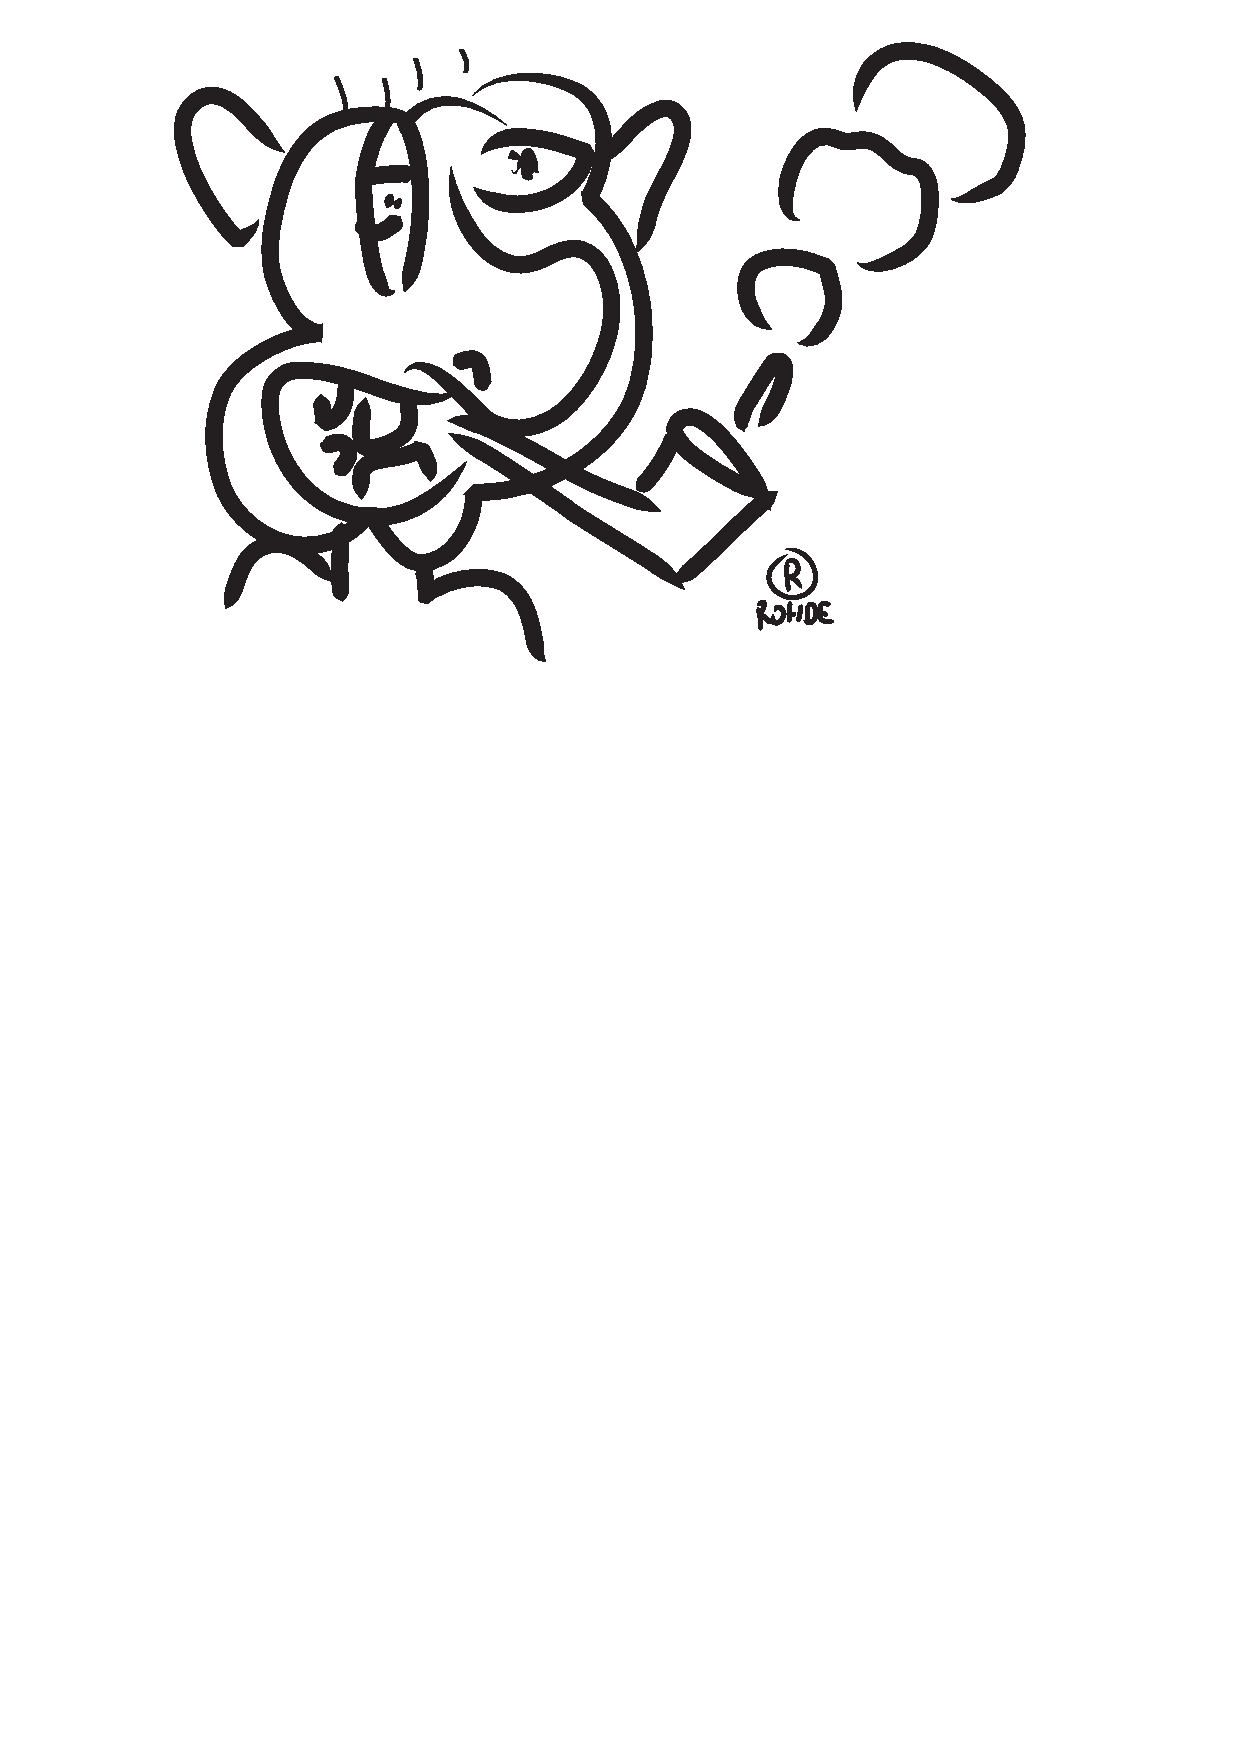
\includegraphics[width=0.8\columnwidth]{cover_picture}
\newpage
The desire to share and unite remote digital assets motivated the development of the classical internet, the enabler of the entire 21st century economy and our modern way of life. As we enter the quantum era, it is to be expected there will be a similar demand for networking quantum assets, motivating a \textit{global quantum internet} for bringing together the world's quantum resources, leveraging off their exponential trajectory in capability. We present models for quantum networking, how they might be applied in the future, and the implications they will have. Socially, economically, politically and geo-strategically, the upcoming era of quantum supremacy will be as significant for the 21st century as the transistor was for the 20th. The inherently different scaling in the computational power of quantum computers fundamentally changes the dynamics of how they will operate in the future. Given their high expected initial cost, a client/server model for outsourcing computation will be essential to enabling the accessibility and proliferation of this technology, and ensuring its economic viability. We therefore anticipate the emergence of \textit{cloud quantum computing}, a model for outsourcing quantum computations to the network. We argue that economic efficiency will mandate that all future quantum computers be united into a single global \textit{virtual quantum computer}, offering exponentially more power to all network participants than if they were to keep their resources to themselves. This model for the allocation of computational resources is uniquely quantum, with no classical analogue, completely altering the economic landscape for the future of computation. Given the sensitivity of much of the data to which future quantum computers are going to be applied, protocols for encrypted quantum computation will be essential -- the outsourcing of computations that neither an eavesdropper nor even the server performing the computation can spy on. This will enable new models for the commercialisation and proliferation of quantum technologies, unlike any existing models for classical computing. While this work is only an early step in a rapidly developing field, still in its infancy, the central concepts we present will be highly relevant to future developments.
\\[4pt]
We present both original ideas, as well as an extensive review of relevant and related background material. The work is divided into technical sections (requiring only a basic knowledge of the notation of quantum mechanics), for those interested in mathematical details, as well as extensive, entirely non-technical sections for the less technically inclined.
\\[4pt]
We target this work very broadly at quantum and classical computer scientists, classical computer systems, software and network engineers, physicists, economists, and those just generally curious about the future of quantum technologies and what it might bring to humanity.
\\[4pt]
\textit{--- Ad astra per alas fideles. Scientia potentia est.}
\newpage
\end{abstract}

%
% Title
%

\maketitle

%
% Table Of Contents
%

\makeatletter
\def\l@paragraph{\@dottedtocline{4}{8em}{1.2em}}
\makeatother

\makeatletter
\addtocontents{toc}{\def\string\@dotsep{100}}
\makeatother

\tableofcontents 
\addtocontents{toc}{~\hfill\textbf{Page}\par}

%
% Foreword
%

\section{Foreword}

Quantum technologies are not just of interest to quantum physicists, but will have transformative effects across countless areas -- the next technological revolution. For this reason, this work is directed at a general audience of not only quantum computer scientists, but also classical computer scientists, physicists, economists, and computer, software and network engineers. More broadly, we hope this work will be of interest to those who recognise the future significance of quantum technologies, and the implications (or even just curiosities) that globally networking them might have.

A basic understanding of quantum mechanics \cite{bib:Sakurai94}, quantum optics \cite{bib:GerryKnight05}, quantum computing and quantum information theory \cite{bib:NielsenChuang00}\footnote{Throughout this manuscript we use the Nielsen \& Chuang convention for the pronunciation of `zed'.\index{Zed}}, and classical networking \cite{bib:TanenbaumNet} are helpful, but not essential, to following our discussion. Some mathematical sections require a basic understanding of the mathematical notation of quantum mechanics. Although the reader without this background ought to be able to nonetheless follow the broader arguments.

The entirely technically disinterested or mathematically incompetent reader may refer to just Secs.~\ref{sec:introduction}, \ref{sec:outlook} \& \ref{sec:vision_quant} -- essentially brief non-technical essays about the motivation, applications and implications of the future quantum internet.

This work is partially a review of existing knowledge relevant to quantum networking, and partially original ideas, to a large extent based on the adaptation of classical networking concepts and quantum information theory to the context of quantum networking. A reader with an existing background in these areas could calmly skip the respective review sections.

Our goal is to present a broadly accessible technical and non-technical overview of how we foresee quantum technologies to operate in the era of quantum globalisation, and the exciting possibilities that will emerge.

%
% Introduction
%

\section{Introduction} \label{sec:introduction}

The internet is one of the key technological achievements of the 20th century, an enabling factor in every aspect of our everyday use of modern technology. While digital computing was the definitive technology of the 20th century, quantum technologies will be for the 21st \cite{bib:NielsenChuang00, bib:Bennett00}. 

Perhaps the most exciting prospect in the quantum age is the development of quantum computers\index{Quantum computing}. Richard Feynman \cite{bib:Feynman85} was the first to ask the question `If quantum systems are so exponentially complex that we are unable to simulate them on our classical computers, can those same quantum systems be exploited in a controlled way to exponentially outperform our classical computers?'\index{Richard Feynman}. Subsequently, the Deutsch-Jozsa algorithm \cite{bib:DeutschJozsa92}\index{Deutsch-Jozsa algorithm} demonstrated for the first time that algorithms can run on a quantum computer, exponentially outperforming any classical algorithm. Since then, an enormous amount of research has been dedicated to finding new quantum algorithms, and the search has indeed been a very fruitful one\footnote{See the Quantum Algorithm Zoo for a comprehensive summary of the current state of knowledge on quantum algorithms (\texttt{\href{http://math.nist.gov/quantum/zoo/}{http://math.nist.gov/quantum/zoo/}}).}, with many important applications having been found, including, amongst many others\index{Quantum algorithms}:

\begin{itemize}
	\item Searching unstructured databases:\index{Grover's algorithm}
		\begin{itemize}
		\item Grover's algorithm \cite{bib:Grover96}.
		\item Quadratic speedup.
		\end{itemize}
	\item Satisfiability problems\footnote{A satisfiability problem is one where we search a function's input space for a solution(s) satisfying a given output constraint. The hardest such problems, like the archetypal \textsc{3-SAT}\index{3-\textsc{SAT}} problem, are \textbf{NP}-complete.}\index{\textbf{NP} \& \textbf{NP}-complete}:
		\begin{itemize}
			\item Grover's algorithm.
			\item Quadratic speedup.
			\item Includes solving \textbf{NP}-complete problems, and brute-force cracking of private encryption keys\footnote{Note that when performing a brute-force attack against a private encryption key, a quadratic speedup effectively halves the key length in terms of algorithmic runtime. Thus, in the quantum era private key lengths will need to be doubled.}.\index{Satisfiability problems}
			\end{itemize}
	\item Optimisation problems:
		\begin{itemize}
			\item Grover's algorithm.
			\item Quadratic speedup.
			\item Many optimisation problems reside in \textbf{NP} or can be approximated in \textbf{NP}.\index{Optimisation problems}
			\end{itemize}
	\item Period finding and integer factorisation\index{Shor's algorithm}:
		\begin{itemize}
		\item Shor's algorithm \cite{bib:ShorFactor}.
		\item Exponential speedup.
		\item This compromises Rivest, Shamir \& Adleman (RSA) public-key cryptography \cite{bib:RSA}\index{RSA encryption}, the most widely used cryptographic protocol on the internet today.
		\end{itemize}
	\item Simulation of quantum systems\index{Quantum simulation}:
		\begin{itemize}
			\item Lloyd's algorithm \cite{bib:lloyd1996universal}.
			\item Exponential speedup.
			\item This includes simulation of: molecular and atomic interactions in the study of quantum chemistry or nuclear physics; interactions between drug molecules and organic molecules for drug design; genetic interactions for the study of genetics and genetic medicine; nanoscale semiconductor physics for integrated circuit design; and much more.
			\end{itemize}
	\item Simulation of quantum field theories\index{Simulating quantum field theories}:
		\begin{itemize}
		 \item Jordan-Lee-Preskill algorithm \cite{bib:JLP, bib:RohdeWavelet15}
		 \item Exponential speedup.
		 \item A key area of fundamental physics research.
		 \end{itemize}
	\item Topological big-data analysis\index{Topological big-data analysis}
		\begin{itemize}
		\item Lloyd's algorthm \cite{bib:lloyd2016quantum, USTCexperiment}.
		\item Exponential speedup.
		\item Broad applications including: social media network analysis; consumer behaviour; behavioural dynamics; neuroscience; and higher-dimensional signal and image processing.
		\end{itemize}
	\item Solving linear systems of equations\index{Linear systems}
		\begin{itemize}
		\item \comment{To do} \cite{bib:harrow2009quantum, bib:BerryLinear}.
		\item Exponential speedup.
		\item Widespread applications in linear algebra and calculus.
		\end{itemize}
	\item Quantum machine learning\index{Quantum machine learning}
		\begin{itemize}
		\item Lloyd's algorithm \cite{bib:lloyd2013quantum}.
		\item This includes putting an end to humanity.
		\item \textit{Ne obliviscaris}.
		\end{itemize}
\end{itemize}

It is likely we haven't yet begun to fully recognise the capabilities of quantum computers, and the full plethora of applications they may have in the future. We stand at the beginning of the emergence of an entirely new type of technology.

In addition to many practical applications, the onset of quantum computing carries with it deep philosophical implications. Specifically, the Extended Church-Turing (ECT)\index{Extended Church-Turing thesis} thesis hypothesises that any physically realisable system can be \textit{efficiently}\footnote{The term `efficient' is coined by the computer scientist to mean that a problem can be solved in time at most polynomial in the size of the problem.\index{Computational efficiency}} simulated by a universal Turing machine\index{Turing machines} (i.e classical computer). The believed exponential complexity of quantum systems inclines quantum computer scientists to believe that the ECT thesis is therefore false \cite{bib:Deutsch85}\footnote{We have discovered a truly marvelous proof of this, which this footnote is too narrow to contain.}. The demonstration of large-scale quantum computers, while unable to prove or disprove the ECT thesis\footnote{When one talks about `scalability' or the `ECT thesis', we are talking about asymptotic relationships. Clearly no finite-sized experiment can prove asymptotic scaling with certainty. But with a sufficiently large quantum computer at our disposal, demonstrating exponentially more computational power than its classical sibling, we might be reasonably satisfied in convincing ourselves about the nature of the scaling of different computational models.}, could at least provide some convincing evidence against the ECT conjecture.

From a computational complexity\index{Computational complexity theory} theorist's perspective, it is strongly believed that the complexity classes of problems efficiently solvable on classical computers (\textbf{P} \& \textbf{BPP}\index{\textbf{P} \& \textbf{BPP}}) and quantum computers (\textbf{BQP}\index{\textbf{BQP} \& \textbf{BQP}-complete}) are distinct. Specifically, it is believed that \mbox{$\mathbf{BPP}\subset\mathbf{BQP}$}. If this conjecture is correct, it implies the existence of quantum algorithms super-polynomially faster than the best classical ones, and that the ECT thesis is not correct. More specifically, Fig.~\ref{fig:complexity_classes} illustrates the believed relationships between some of the most important complexity classes relevant to quantum computing.

\begin{figure}[!htb]
	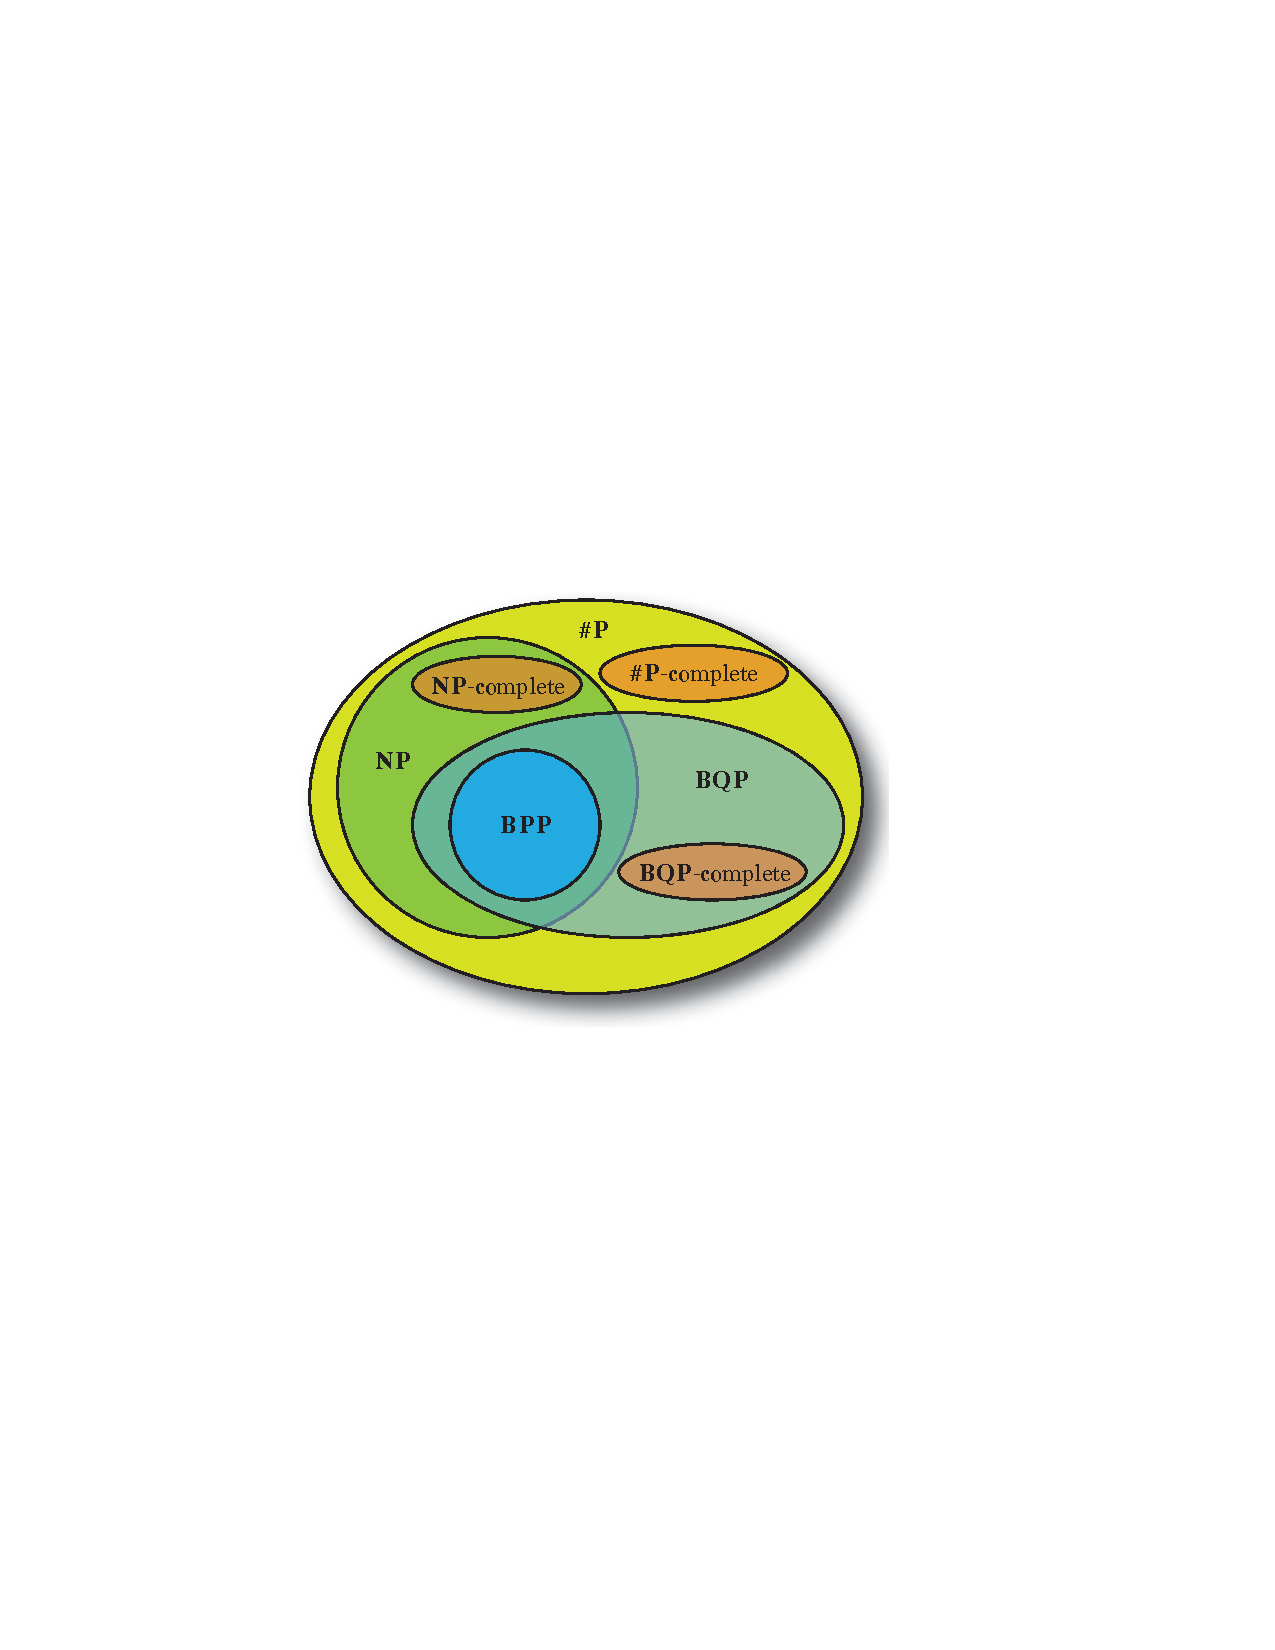
\includegraphics[width=\columnwidth]{complexity_classes}\index{Complexity classes} \index{\textbf{P} \& \textbf{BPP}} \index{\textbf{NP} \& \textbf{NP}-complete} \index{\textbf{BQP} \& \textbf{BQP}-complete} \index{\textbf{\#P} \& \textbf{\#P}-complete}
	\caption{Believed relationships between the complexity classes most relevant to quantum computing. \textbf{BPP} is the class of polynomial-time probabilistic classical algorithms. \textbf{NP} is the class of problems verifiable in polynomial time using classical algorithms. \textbf{NP}-complete are the subset of \textbf{NP} problems polynomial-time reducible to any other problem in \textbf{NP}. \textbf{BQP} is the class of probabilistic algorithms solvable in polynomial time on universal quantum computers. $\#\mathbf{P}$ is the set of counting problems, that count satisfying solutions to \textbf{P} problems (\textbf{P} is the same as \textbf{BPP}, but deterministic, rather than probabilisitic). Note that it is actually unproven whether \mbox{$\mathbf{P}=\mathbf{BPP}$} or \mbox{$\mathbf{P}\subset\mathbf{BPP}$}. There are examples where the best known \textbf{BPP} algorithms outperform the best known \textbf{P} algorithms, which could arise because the two classes are inequivalent, or that we simply haven't tried hard enough to find the best deterministic algorithms. Furthermore, while it is known that \mbox{$\mathbf{P}\subseteq\mathbf{NP}$}, it is not known whether \mbox{$\mathbf{BPP}\subseteq\mathbf{NP}$}. For the sake of illustration in our Venn diagram we have taken the view that it is. \textbf{BPP} is regarded as the class of problems efficiently solvable on universal Turing machines (i.e classical computers), whereas \textbf{BQP} is that efficiently solvable on universal quantum computers. The computational superiority of quantum computers is based on the (strongly believed, yet unproven) assumption that \mbox{$\mathbf{BPP}\subset\mathbf{BQP}$}.} \label{fig:complexity_classes}
\end{figure}

Aside from quantum computing, quantum cryptography\index{Quantum cryptography} holds the promise of uncrackable cryptographic protocols, guaranteed not by the assumed complexity of solving certain mathematical problems like integer factorisation or brute-force searching, but by the laws of quantum mechanics. That is, provided our understanding of quantum mechanics is correct, quantum cryptographic protocols exist, which cannot be cracked, irrespective of the computational resources of an adversary.

Already we are beginning to see elementary realisations of essential quantum technologies such as quantum computing, cryptography, and metrology. As these technologies become increasingly viable and more ubiquitous, the demand for networking them and sharing quantum resources between them will become a pressing issue. Most notably, quantum cryptography and \textit{cloud quantum computing} will be pivotal in the proliferation of quantum technology, which necessarily requires reliable quantum communications channels.

The first demonstrations of digital computer networks were nothing more than simple two-party, point-to-point (P2P) communication. However, the internet we have today extends far beyond this, allowing essentially arbitrary worldwide networking across completely ad hoc networks comprising many different mediums, with any number of parties, in an entirely plug-and-play and decentralised fashion. Similarly, elementary demonstrations of quantum communication\index{Quantum communication} have been performed across a small number of parties, and much work has been done on analysing quantum channel capacities in this context \cite{??? channel_capacity}. But, as with digital computing, demand for a future \textit{quantum internet} is foreseeable, enabling the arbitrary communication of quantum resources, between any number of parties, over ad hoc networks.

The digital internet may be considered a technology stack, such as TCP/IP (Transmission Control Protocol/Internet Protocol)\index{Transmission Control Protocol/Internet Protocol (TCP/IP)}, comprising different levels of abstraction of digital information \cite{bib:TanenbaumNet}. At the lowest level we have raw digital data we wish to communicate across a physical medium. Above this, we decompose the data into packets. The packets are transmitted over a network, and TCP is responsible for routing the packets to their destination, and guaranteeing data integrity and Quality of Service (\textsc{QoS}). Finally, the packets received by the recipient are combined and the raw data reconstructed.

The TCP layer remains largely transparent to the end-user, enabling virtual software interfaces to remote digital assets that behave as though they were local. This allows high-level services such as the File Transfer Protocol (FTP), the worldwide web, video and audio streaming, and outsourced computation on supercomputers, as though everything was taking place locally, with the end-user oblivious to the underlying networking protocols. To the user, YouTube videos or Spotify tracks behave as though they were held as local copies. And FTP or DropBox allow storage on a distant data centre to be mounted as though it were a local volume. We foresee a demand for these same criteria in the quantum era.

In the context of a quantum internet, packets of data will instead be quantum states, and the transmission control protocol is responsible for guiding them to their destination and ensuring quality control.

Here we present a treatment for such Quantum Transmission Control Protocols (QTCPs)\index{Quantum Transmission Control Protocol (QTCP)} as a theoretical foundation for a future quantum internet. We consider how such ad hoc networks may be described mathematically, how to quantify network performance, and present a QTCP stack for operating it. While the goals of QTCP are similar as for classical TCP, there are major conceptual differences between the classical and quantum internets, owing to the unique properties of quantum states with no classical analogue.

Our treatment of quantum networks will be optics-heavy, based on the reasonable assumption that communications channels will almost certainly be optical, albeit with many possible choices of optical states and mediums. However, this does not preclude non-optical systems from representing quantum information that is not in transit, and we consider such `hybrid' architectures in detail, as well as the interfacing between optical and non-optical systems. Indeed, it is almost certain that future large-scale quantum computers will not be all-optical, necessitating interfacing different physical architectures. We accommodate for this requirement in the design of the QTCP.

Shared quantum entanglement\index{Quantum entanglement} is a primitive resource with direct applications in countless protocols. This warrants special treatment of quantum networks, which do not implement a full QTCP network stack, but instead specialise in just this one task -- entanglement distribution. We will see that such a specialised network will already be immensely useful for a broad range of applications, and its simplicity brings with it many inherent advantages.

The quantum internet will enable advances in the large-scale deployment of quantum technologies. Most notably, in the context of quantum computing it will allow initially very expensive technology to be economically viable and broadly accessible via the outsourcing of computations from consumers who can't afford quantum computers, to well-resourced hosts who can -- \textit{cloud quantum computing}\index{Cloud quantum computing}.

With the addition of recent advances in homomorphic encryption and blind quantum computing\index{Encrypted quantum computation}, such cloud quantum computing can be performed securely, guaranteeing privacy of both data and algorithms, secure even against the host performing the computation. This opens up entirely new economic models and applications for the licensing of compute time on future quantum computers in the cloud.

The unique behaviour of quantum computing, in terms of the super-classical scaling in its computational power, brings with it many important economic and strategic considerations that are extremely important to give attention to in the post-classical world.

But quantum technologies extend far beyond computation. Many other exciting applications for controlled quantum systems exist, with new ones frequently emerging. Thus, the quantum internet will find utility beyond cloud quantum computing, enabling the global exchange of quantum resources and assets. This could include the networking of elementary quantum resources such as state preparation, entanglement sharing, teleportation and quantum measurements, or scale all the way up to massively distributed quantum computation or a global quantum cryptography network.\index{Quantum assets}

It is hard to foresee the future trajectory of quantum technology, much as no one foresaw the advances digital technology has made over the last half century. But it is certain that as the internet transformed digital technology, the quantum internet will define the future of quantum technologies.

%
% Models For Quantum Computation
%

\section{Models for quantum computation} \label{sec:models_QC} \index{Models for quantum computation}

There are various approaches to implementing and representing quantum computations. We now briefly introduce the ones most relevant to our discussions on networked quantum computation. Other formalisms, such as adiabatic quantum computation \cite{???} and quantum simulated annealing \cite{???}, which are not so applicable to networking, will not be introduced, although many excellent introductions to these fields exist \cite{???}.

%
% Quantum Circuits
%

\subsection{Circuit model} \label{sec:circuit_model} \index{Circuit model}

The \textit{circuit model} is the conventional and most intuitive approach for expressing quantum algorithms, decomposing them into chronological sequences of elementary operations, comprising state preparation, single- and multi-qubit gates, measurement, and classical feedforward. We recommend referring to the introductory sections of \cite{bib:NielsenChuang00} for a far more comprehensive introduction to quantum circuits than is presented here. This model will be naturally intuitive to those familiar with classical circuit diagrams, albeit with some important differences, such as time-ordering.

\begin{figure}[!htb]
	\begin{align}
		\Qcircuit @C=.7em @R=.4em @! {
		\lstick{\ket{\psi_1}} & \qw & \qw & \ctrl{1} & \gate{Y} & \meter & \control \cw\\
		\lstick{\ket{\psi_2}} & \qw & \targ & \ctrl{-1} & \qw & \meter & \cwx\\
		\lstick{\ket{\psi_3}} & \gate{H} & \ctrl{-1} & \qw & \qw & \gate{X} \cwx & \gate{Z} \cwx & \rstick{\ket{\phi}} \qw
		} \nonumber
	\end{align}
	\caption{Simple example of a quantum circuit, comprising several single- and two-qubit quantum gates and measurements. Rows represent qubits, and time flows from left-to-right.} \label{fig:eg_circuit}
\end{figure}

Fig.~\ref{fig:eg_circuit} illustrates a simple 3-qubit quantum circuit comprising all of these elements. The interpretation of this diagram is as follows:
\begin{itemize}
	\item Horizontal lines represent individual qubits.
	\item Time flows from left to right (feedback is not allowed in the typical formalism for this representation).
	\item The three input qubits are labelled on the far-left as $\ket{\psi_1}$, $\ket{\psi_2}$ and $\ket{\psi_3}$.
	\item Single-qubit gates are denoted as boxes containing the name of the associated unitary operation. Here, the examples are the Hadamard ($\hat{H}$), Pauli bit-flip ($\hat{X}$), Pauli bit-phase-flip ($\hat{Y}$), and Pauli phase-flip ($\hat{Z}$) gates\index{Pauli gates}\index{Hadamard gate},
	\begin{align}
		\hat{H} &= \frac{1}{\sqrt{2}}\begin{pmatrix}
		1 & 1 \\
		1 & -1
		\end{pmatrix},\nonumber \\
		\hat{X} &= \begin{pmatrix}
		0 & 1 \\
		1 & 0
		\end{pmatrix},\nonumber \\
		\hat{Y} &= \begin{pmatrix}
		0 & -i \\
		i & 0
		\end{pmatrix},\nonumber \\
		\hat{Z} &= \begin{pmatrix}
		1 & 0 \\
		0 & -1
		\end{pmatrix}.
	\end{align}
	\item Two-qubit gates are denoted by vertical lines between the respective qubits.
	\item The maximally-entangling two-qubit controlled-NOT (CNOT) gate\index{Controlled-NOT (CNOT) gate} is denoted via a control ($\bullet$) and a target ($\oplus$),
	\begin{align}
		\hat{\text{CNOT}}=\begin{pmatrix}
		1 & 0 & 0 & 0 \\
		0 & 1 & 0 & 0 \\
		0 & 0 & 0 & 1 \\
		0 & 0 & 1 & 0
		\end{pmatrix}.
	\end{align}
	This is the quantum equivalent of the classical XOR gate.
	\item All quantum gates have the same number of input as output qubits. This is a necessary condition for the unitarity of quantum gates (\mbox{$\hat{U}^\dag \hat{U} = \hat{\mathbb{I}}$}).
	\item The maximally-entangling two-qubit controlled-phase (CZ)\index{Controlled-Z (CZ) gate} gate is denoted by two targets ($\bullet$) (the gate operates symmetrically on its two qubits),
	\begin{align}
		\hat{\text{CZ}}=\begin{pmatrix}
		1 & 0 & 0 & 0 \\
		0 & 1 & 0 & 0 \\
		0 & 0 & 1 & 0 \\
		0 & 0 & 0 & -1
		\end{pmatrix}.
	\end{align}
	\item The `meter' symbol represents a classical measurement in the Pauli $\hat{Z}$-basis (the computational or logical basis).
	\item Double lines represent classical feedforward of measurement outcomes, controlling a subsequent gate.
\end{itemize}

The circuit in Fig.~\ref{fig:eg_circuit} can be interpreted mathematically as implementing the following operation,
\begin{align}
	\ket\phi &= {\hat{Z}_3}^{m_1} \cdot {\hat{X}_3}^{m_2} \cdot \hat{M}_2 \cdot \hat{M}_1 \cdot \hat{Y}_1 \nonumber \\
	&\cdot \hat{\text{CZ}}_{1,2} \cdot \hat{\text{CNOT}}_{3,2} \cdot \hat{H}_3 \cdot \ket{\psi_1}\otimes\ket{\psi_2}\otimes\ket{\psi_3},
\end{align}
where $m_1$ and $m_2$ are the binary measurement outcomes of the two single-qubit $\hat{Z}$-basis measurements, $\hat{M}_1$ and $\hat{M}_2$.

Using the circuit model, arbitrary quantum computations can be elegantly and intuitively represented. To enable \textit{universal} quantum computation within this model, a \textit{universal gate set} must be available at our disposal. Most commonly, this is chosen to be the maximally-entangling two-qubit CZ or CNOT operation, in addition to arbitrary single-qubit gates. Any quantum (i.e \textbf{BQP}) algorithm may be efficiently decomposed into a polynomial-depth circuit comprising elements from this universal gate set.\index{Universal gate sets}

%
% Cluster States
%

\subsection{Cluster states} \label{sec:CSQC} \index{Cluster state model}

The \textit{cluster state} model for quantum computation \cite{bib:Raussendorf01, bib:Raussendorf03, bib:Nielsen06} (also referred to as the \textit{one-way}, \textit{measurement-based}, or \textit{graph state} models for quantum computation) is an extremely powerful paradigm that warrants treatment of its own, owing to its significant distinction from the more familiar circuit model, and its applicability to distributed models for quantum computation, to be discussed in Sec.~\ref{sec:dist_QC}.

In the cluster state model, we begin by preparing a particular, highly-entangled state, called a \textit{cluster state} or \textit{graph state}. The state is associated with a graph $G$, comprising vertices, $V$, and edges, $E$,
\begin{align}
	G=(V,E),
\end{align}
of some topology, although rectangular lattice graphs are usually considered as they are sufficient for universal quantum computation\footnote{Note that the graph upon which a cluster state resides is not to be confused with the network graph. Rather it is just a convenient graphical representation for a class of multi-qubit states.}. That is, they act as a `substrate' for implementing arbitrary quantum computations.

In the graph, vertices represent qubits initialised into the,
\begin{align}
	\ket{+}=\frac{1}{\sqrt{2}}(\ket{0}+\ket{1}),
\end{align}
state, and edges represent the application of maximally entangling CZ gates between vertices,
\begin{align}
	\ket\psi_\text{cluster} = \prod_{e\in E} \hat{\text{CZ}}_e \cdot \bigotimes_{v\in V}\ket{+}_v.
\end{align}
Alternately, but equivalently, cluster states may be defined in the stabiliser formalism\index{Stabiliser formalism}. Specifically, a cluster state is defined to be the joint +1 eigenstate of all the stabilisers,
\begin{align} \label{eq:CS_stab} \index{Cluster state stabilisers}
	\hat{S}_v = \hat{X}_v \prod_{i\in n_v} \hat{Z}_i,
\end{align}
where there is one stabiliser $\hat{S}_v$ per vertex $v$, and $n_v$ is the set of vertices neighbouring $v$. The cluster state therefore satisfies,
\begin{align}
	\hat{S}_v\ket\psi_\text{cluster} = \ket\psi_\text{cluster}\,\forall\, v,
\end{align}
and the full set of stabilisers, $\hat{S}_v$, over all vertices $v$ is sufficient to fully characterise the cluster state, $\ket{\psi}_\text{cluster}$, for a given graph topology.

An example of a rectangular lattice cluster state is presented in Fig.~\ref{fig:cluster_state}. Cluster states are easily encoded optically using photonic polarisation encoding (Sec.~\ref{sec:single_phot_enc}), and therefore readily lend themselves to optical networking.

\begin{figure}[!htb]
	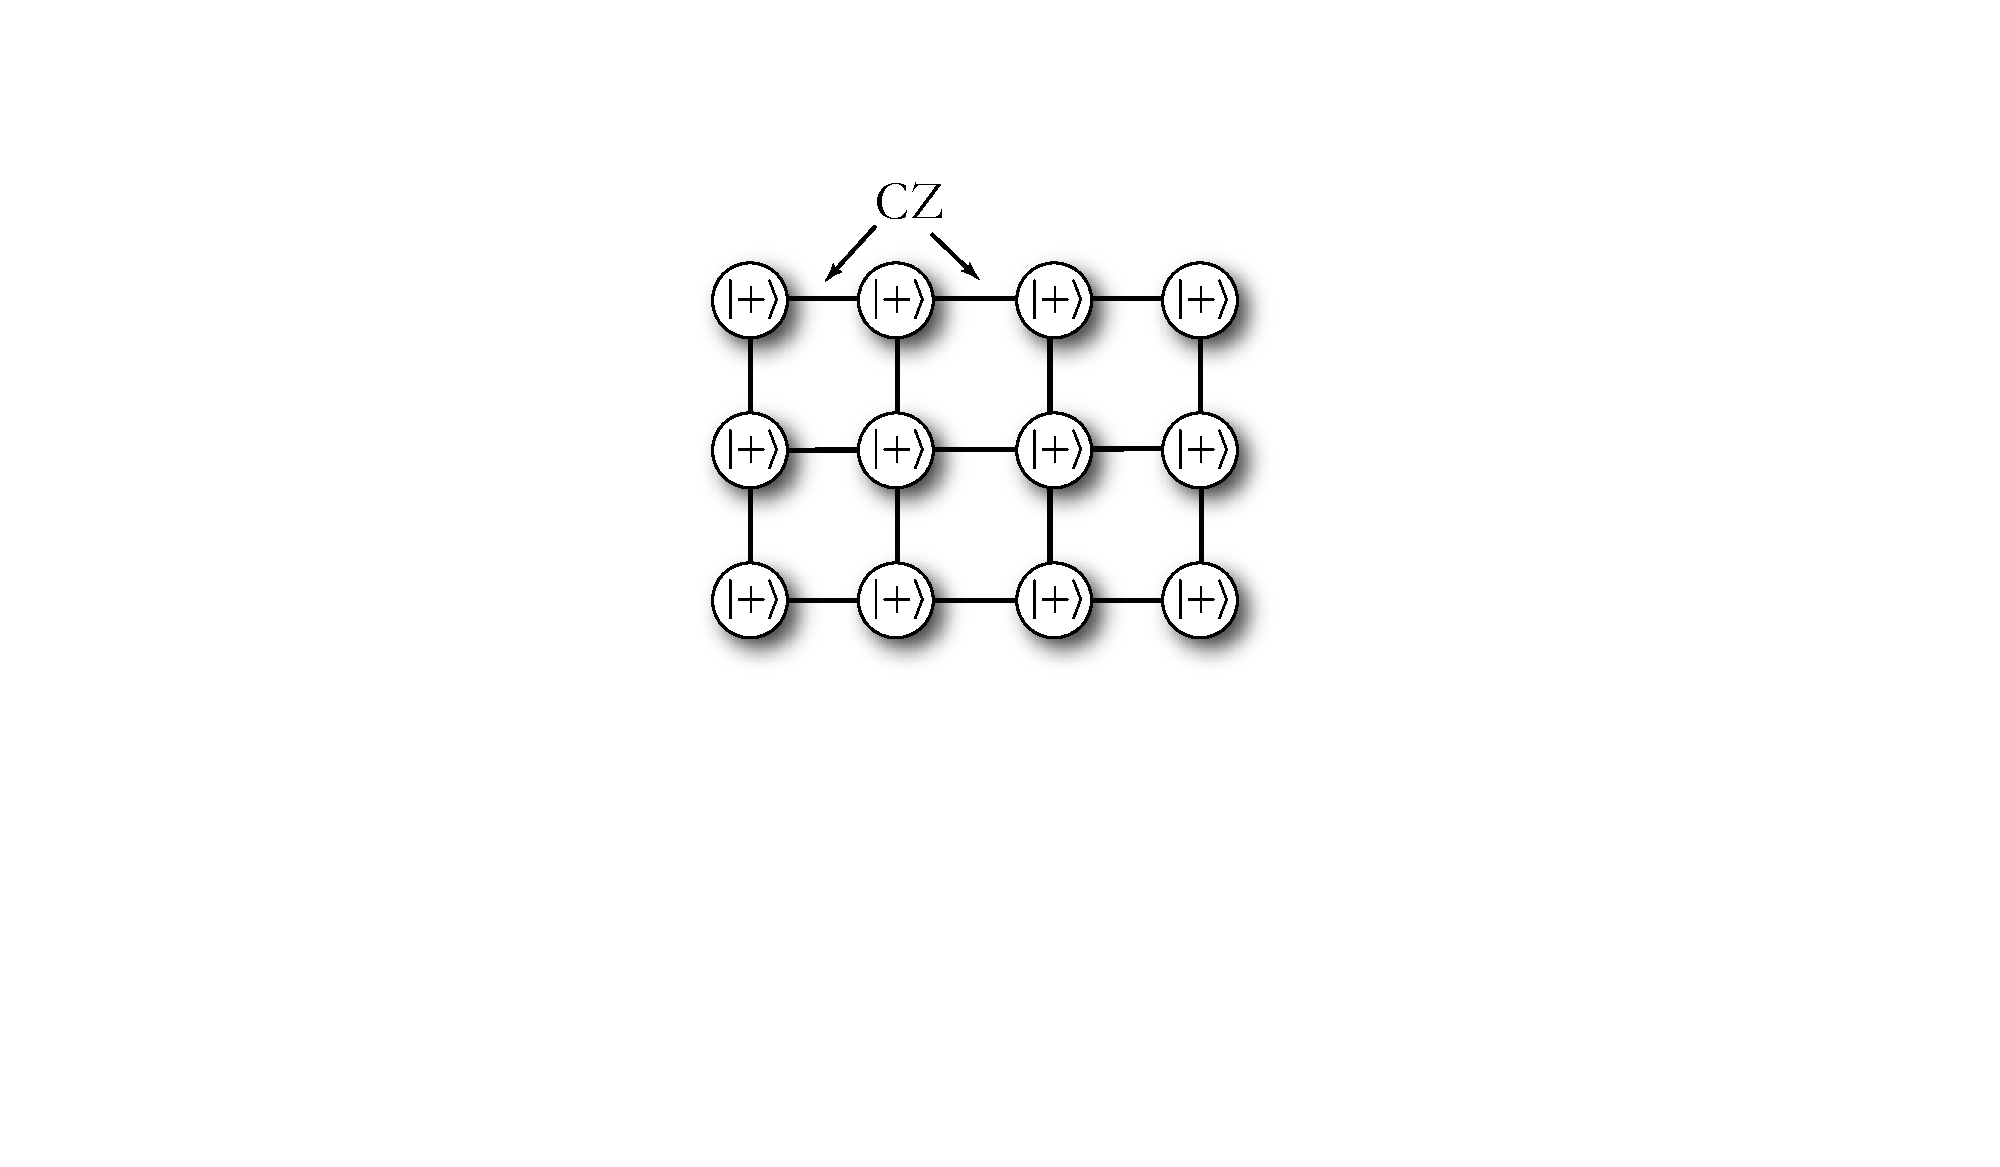
\includegraphics[width=0.6\columnwidth]{cluster_state}
	\caption{Example of a \mbox{$4\times 3$} rectangular lattice cluster state. Each vertex in the graph represents a qubit initialised into \mbox{$\ket{+}=\frac{1}{\sqrt{2}}(\ket{0}+\ket{1})$}. Edges represent the application of CZ gates between qubits (CZ gates commute, so the order is unimportant). Of sufficient dimension, states of this topology enable universal measurement-based quantum computation, whereby computation proceeds purely via single-qubit measurements, and all entangling operations have been commuted to the state preparation stage. Because CZ gates commute, the preparation of cluster states is time-independent, and easily implemented in a distributed or parallelised manner. The time-ordering of the single-qubit measurements is dependent on the structure of the graph and the algorithm.} \label{fig:cluster_state}
\end{figure}

Having prepared this state, the computation is implemented purely via a well-orchestrated routine of single-qubit measurements. The order and basis in which they are performed (which depends on previous measurement outcomes in general -- i.e we require fast-feedforward) then stipulates the computation. In the context of distributed computation (Sec.~\ref{sec:dist_QC}), this requires classical communication between nodes.

Mapping a circuit model computation to a cluster state topology can be most na{\" i}vely performed by taking a circuit acting on $n_\text{qubits}$ qubits with depth $n_\text{depth}$, preparing an \mbox{$n_\text{qubits}\times n_\text{depth}$} rectangular lattice cluster, and `etching' the circuit directly into the cluster state substrate. To perform this mapping we choose a universal gate set comprising CZ and single-qubit gates, retaining vertical edges where CZ gates ought to be present, eliminating the remaining vertical edges. Now we have a substrate that looks topologically very much like its equivalent circuit construction, and the computation proceeds chronologically in the same manner. The only conceptual distinction is that in the circuit model gates are directly applied chronologically to the set of qubits, whereas in the cluster state gate teleportation (Sec.~\ref{sec:teleport_gate}) is effectively implemented upon each measurement, with the action of gates accumulating as these teleportations are successively applied. A simple example of this notion is shown in Fig.~\ref{fig:cluster_state_circuit}.

\begin{figure}[!htb]
	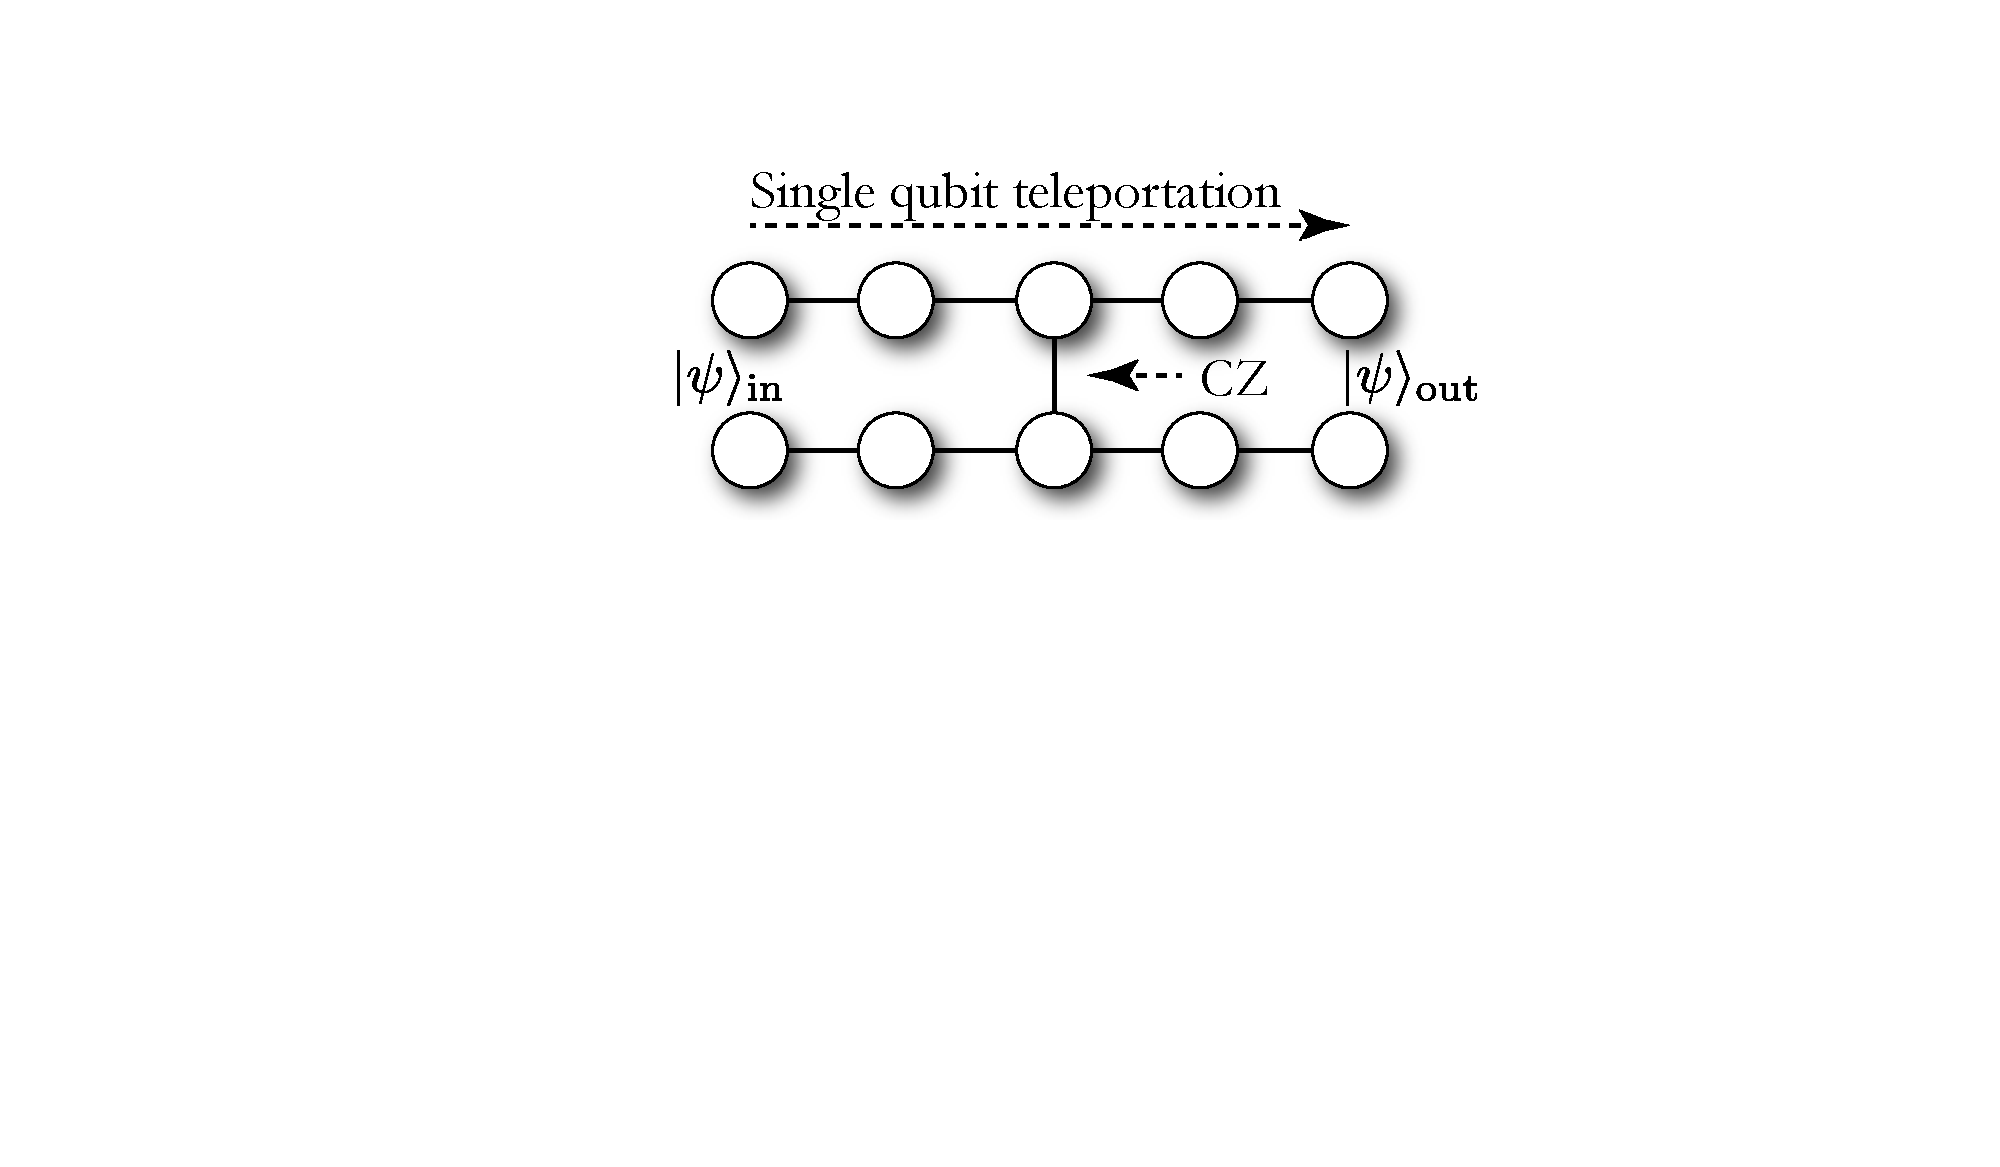
\includegraphics[width=0.75\columnwidth]{cluster_state_circuit}
	\caption{Simple example of a cluster state that performs a computation comprising single-qubit operations and a CZ gate between two logical qubits. Let the two horizontal chains represent our two logical qubits. After inputting our input state from the left, we progressively measure out the cluster state qubits chronologically from left-to-right. Upon each single-qubit measurement, the choice of measurement basis teleports the action of a single-qubit gate. These accumulate sequentially. When we reach the point of measuring the two cluster state qubits joined with the vertical edge, the logical qubits accumulate the action of a CZ gate between them, since this is identically what that vertical edge physically corresponds to. Reaching the final two qubits, one from the upper rail and one from the lower, we obtain our two output logical qubits.} \label{fig:cluster_state_circuit}
\end{figure}

The distinctive feature of this model is that all the entangling CZ gates are performed at the very beginning of the protocol, during the state preparation stage. The algorithm itself is purely measurement-based, requiring only single-qubit measurements (no entangling measurements).

An alternate interpretation of the cluster state model is that it is a complicated network of state and gate teleportation protocols (Sec.~\ref{sec:teleport}). Specifically, a CZ gate with a $\ket{+}$ state as a resource, followed by measurement of one of the two qubits acts as a single-qubit teleporter, as shown in Fig.~\ref{fig:single_qubit_teleporter}\footnote{This is an alternative, but equivalent implementation for quantum state teleportation to that presented in Sec.~\ref{sec:teleport}.}. Thus, with a substrate state of CZ gates applied between $\ket{+}$ states, the single-qubit measurements progressively teleport the input state through the graph topology, at each stage accumulating the action of more gates, which are related to the choices of the previous single-qubit measurement bases, and the graph topology.

\begin{figure}[!htb]
	\begin{align}
		\Qcircuit @C=.7em @R=.4em @! {
		\lstick{\ket{\psi}} & \ctrl{1} & \gate{H} & \meter & & \\
		\lstick{\ket{+}} & \ctrl{0} & \qw & \gate{X} \cwx & \gate{H} & \rstick{\ket\psi} \qw \\
		} \nonumber
	\end{align}
	\caption{The single-qubit teleporter, based upon a CZ gate, a single-qubit measurement, and classical feedforward.} \label{fig:single_qubit_teleporter} \index{Single-qubit teleporter}
\end{figure}

The cluster state formalism has proven very useful, enabling the development of linear optics quantum computing (Sec.~\ref{sec:KLM_univ}), orders of magnitude more efficient than the originally proposed protocol for linear optics quantum computing. It has been found that bonding strategies -- i.e the order in which smaller clusters are fused into larger ones when using non-deterministic gates -- plays a major role in resource overhead, and much work has been performed on efficient preparation strategies for various topologies \cite{bib:Nielsen04, bib:BarrettKok05, bib:BrowneRudolph05, bib:BenjaminEisert05, bib:Gross06, bib:RohdeStratCS07, bib:Kieling06, bib:KielingRudolphEisert06, bib:RohdeBarrett07, bib:Kieling07, bib:Campbell07, bib:Campbell07b}.

These cluster states are highly valuable, given their computational power, and the ability to communicate them from Alice, who is able to prepare them, to Bob, who lacks the technology, would be a boon for Bob.

It would be most practical, economical, and resource efficient to have a single, well-equipped server with the ability to prepare such states, who does so on behalf of everyone else, and communicates the fresh cluster states to them over the quantum internet (for a price, perhaps).

Importantly, the preparation of cluster states is readily parallelised. All the entangling CZ operations commute, the order in which they are applied is irrelevant, and a rectangular lattice cluster is completely uniform. Thus, the graphs representing smaller cluster states may be easily `fused' together to form larger cluster states using, for example, CZ gates. Several other types of entangling gates can also be employed, such as polarising beamsplitters -- so-called \textit{fusion gates} \cite{bib:BrowneRudolph05}. This allows the preparation of cluster states to be performed in a `patchwork quilt'-like manner -- a number of nodes each prepare small lattice clusters, they are all put side-by-side, and stitched together using CZ gates. This type of distributed state preparation is a perfect application for in-parallel distributed quantum processing.

Consider the scenario whereby Alice requests a large cluster state from Bob, but, while she was unable to prepare the cluster state herself, she has the technological ability to perform the measurement-based computation on the state (i.e single-qubit measurements). This would effectively bypass the need for blind/homomorphic quantum computation on Bob's hardware altogether, enabling computation with \textit{perfect} secrecy, since no foreign parties would be involved in the computation stage, and no secret data is communicated -- only the \textit{substrate} for the computation is communicated, which could be used for any purpose whatsoever. By commuting all the technologically challenging aspects of a quantum computation to the state preparation stage, we can effectively mitigate the need for blind quantum computing entirely, since the `hard work' has been done in advance by the host, and Alice gets to fulfil the computation on her own, completely bypassing poor old Bob, who was just dying to read Alice's secret love letters before processing them into Hallmark cards.

There are several cluster state identities we will utilise later, summarised in Fig.~\ref{fig:cluster_ident}.

\begin{figure}[!htb]
	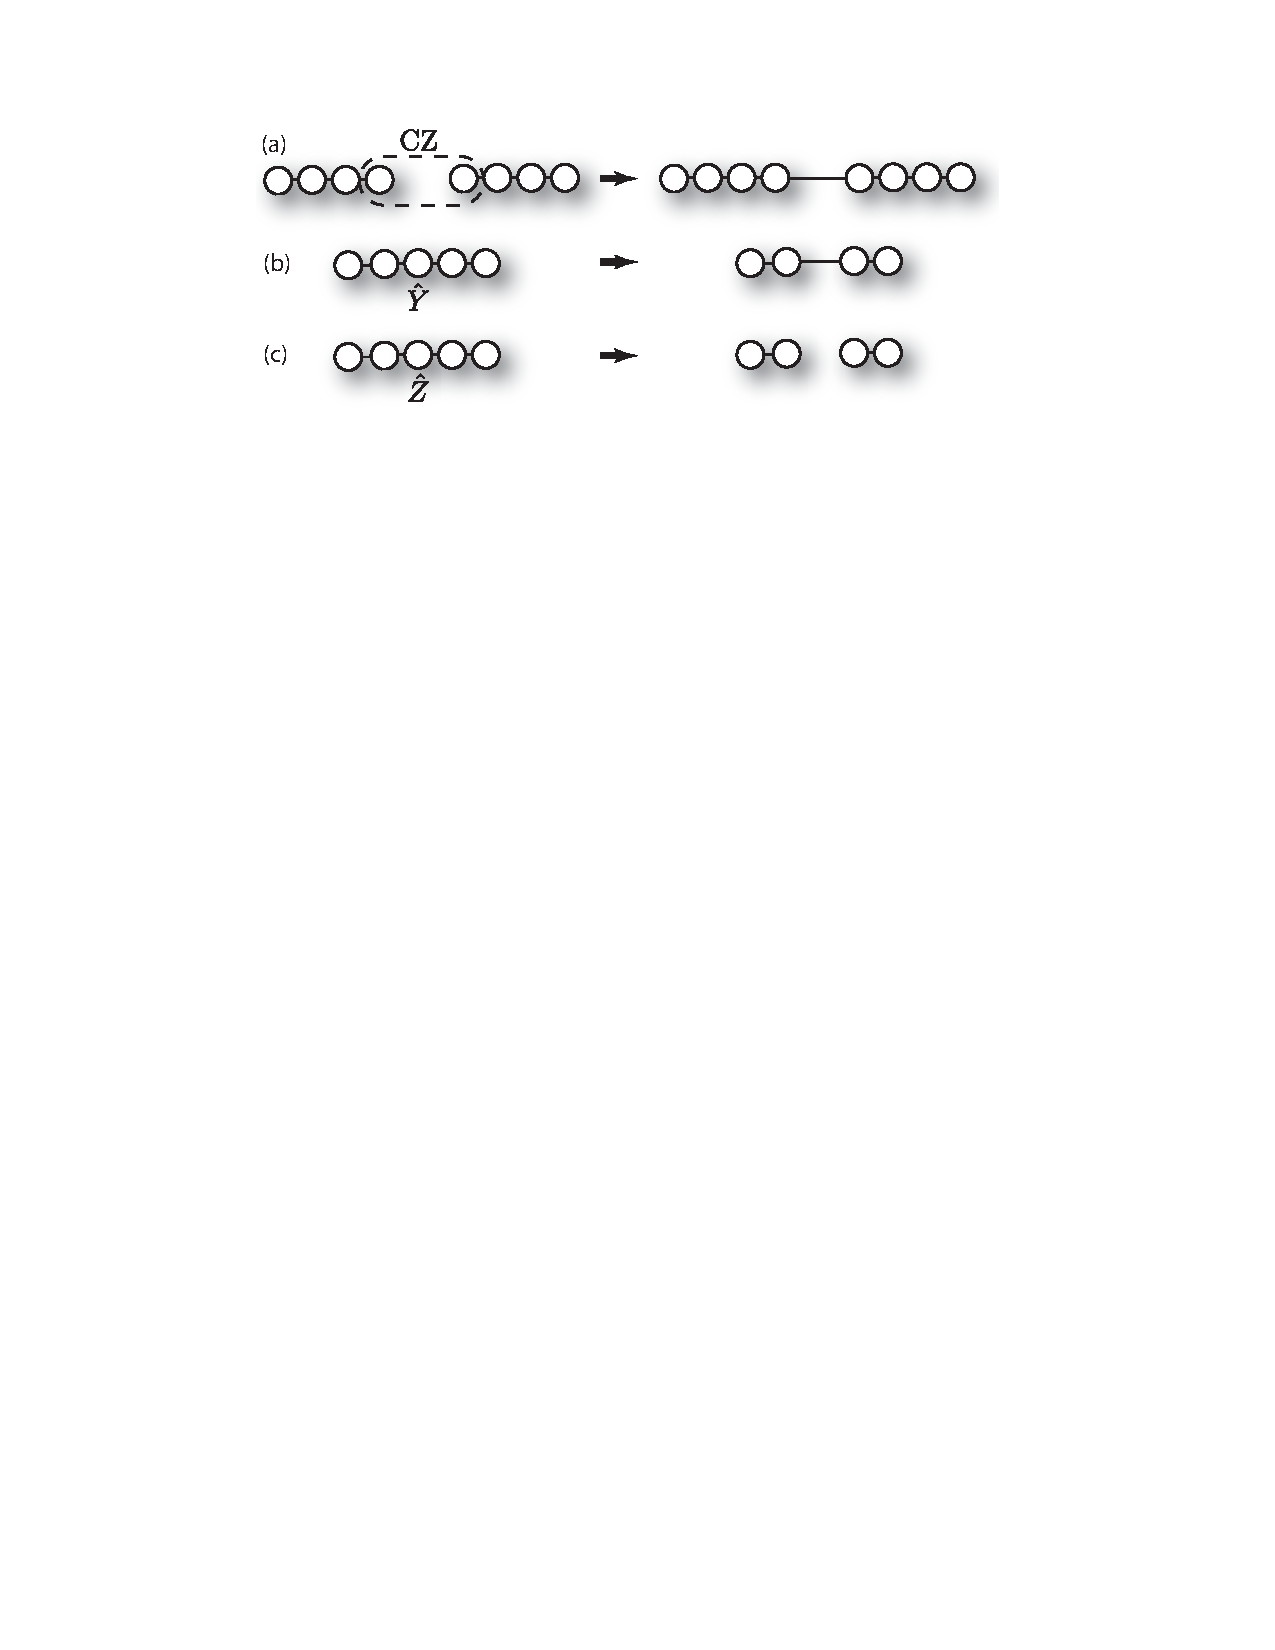
\includegraphics[width=\columnwidth]{cluster_identities} \index{Cluster state identities}
	\caption{Several cluster state identities. (a) a CZ gate between two qubits creates an edge between them in the graph. (b) Measurement of a qubit in the Pauli $\hat{Y}$ basis removes that qubit from the graph, while creating new edges between the neighbouring qubits. (c) Measurement of a qubit in the Pauli $\hat{Z}$ basis removes that qubit and any neighbouring edges.} \label{fig:cluster_ident} 
\end{figure}

When using non-deterministic gates to prepare cluster states, there are approaches to nonetheless preparing ideal cluster states. This is discussed in more detail in Sec.~\ref{sec:module}. Alternately, we can borrow ideas from percolation theory\index{Percolation theory} to simply tolerate defects in a cluster state lattice by working around them. Specifically, if the defect probability (i.e probability of a missing vertex or edge) is below some \textit{percolation threshold}\index{Percolation threshold}, \mbox{$p_\text{defect}\leq \epsilon_\text{threshold}$}, in the asymptotic limit we are guaranteed that routes exist through the lattice, enabling the required flow of information. This allows defective graphs to be employed for quantum computation.

%
% Topological Codes
%

\subsection{Topological codes} \label{sec:topol_codes} \index{Topological codes}

If the intention is to perform quantum computations using cluster states shared over a network, QEC and fault-tolerance \textit{must} be taken into consideration, or catastrophic algorithmic failure will inevitably follow -- the cluster state model is no different from the circuit model in this respect. Fault-tolerance theory places hard thresholds on the amount of noise (typically depolarising errors and loss) qubits may be subject to in order for fault-tolerance to be possible and computations to succeed. This places strict QoS (Sec.~\ref{sec:QOS}) constraints on the network, which can be accommodated for using the usual depolarising and efficiency cost metrics when developing networking strategies and link performance requirements.

It has been shown that fault-tolerance is possible within the cluster state model \cite{bib:NielsenDawson04, bib:Dawson06} using variations of conventional QEC codes. However, more importantly, from cluster states certain \textit{topological QEC codes} \cite{???} can be readily constructed. This implements a form of QEC-encoded measurement-based quantum computing protocol, where the computation proceeds in a measurement-based fashion, but is `natively' fault-tolerant.

These codes have been shown to have very favourable fault-tolerance thresholds in terms of both depolarising noise and loss \cite{bib:StaceBarrettDohertyLoss, bib:BarrettStaceFT}, as well as frugal resource overhead compared to traditional concatenated codes. Additionally, loss- and gate-failure-tolerant codes, uniquely applicable to the cluster state model, have been described, with very favourable loss thresholds \cite{bib:Varnava05, bib:RalphHayes05, bib:Duan05}. 

Importantly, topological codes do not require joint measurements across the entire graph state, instead requiring only operations localised to small regions within the graph. Thanks to this, computation using such topological codes can remain distributed, without requiring the entire state to be held locally by a particular host, or requiring full access to the entire state by any particular user.

The most common topological code, which we will use here as an example, is the toric code\index{Toric code}, which resides on a lattice graph over the surface of a torus\footnote{As with cluster states, this graph needn't (but could) correspond to A network graph.}. As with cluster states (Sec.~\ref{sec:CSQC}), the toric code is most easily visualised in the stabiliser formalism\index{Stabiliser formalism}. Consider a rectangular sub-graph of the torus. We place a qubit on each edge (not vertex) of the graph. Now we define two sets of stabiliser operators: \textit{star} and \textit{plaquette} operators,
\begin{align} \index{Topological code stabilisers}\index{Star operator}\index{Plaquette operator}
	\hat{S}_\text{star}(v) &= \prod_{i\in e(v)} \hat{X}_i, \nonumber \\
	\hat{S}_\text{plaquette}(p) &= \prod_{i\in e(p)} \hat{Z}_i,
\end{align}
where $e(v)$ are the edges neighbouring vertex $v$, and $e(p)$ are the edges surrounding plaquette $p$. By definition, the toric code state, $\ket\psi_\text{toric}$, satisfies the stabiliser relations,
\begin{align}
	\hat{S}_\text{star}(v) \ket\psi_\text{toric} &= \ket\psi_\text{toric} \,\forall\, v, \nonumber \\
	\hat{S}_\text{plaquette}(p) \ket\psi_\text{toric} &= \ket\psi_\text{toric} \,\forall\, p.
\end{align}
Unlike the cluster state stabilisers from Eq.~(\ref{eq:CS_stab}), these stabilisers are insufficient to fully characterise a unique quantum state. Rather, there are two unspecified degrees of freedom, which allows for a single qubit to be represented. Modifications of the topology, in the form of holes in the lattice (the genus of the topology), allow larger numbers of qubits to be encoded. Logical operations are implemented by performing gates and measurements across topologies over the surface.

The important feature to note is that logical qubits encoded into the toric code do not reside locally at any of the physical qubits in the topology. Rather, they reside jointly across the entire graph, which, like cluster states, might be partitioned across multiple hosts, enabling distributed computation.

This is all summarised in Fig.~\ref{fig:toric_code}.

\begin{figure}[!htb]
	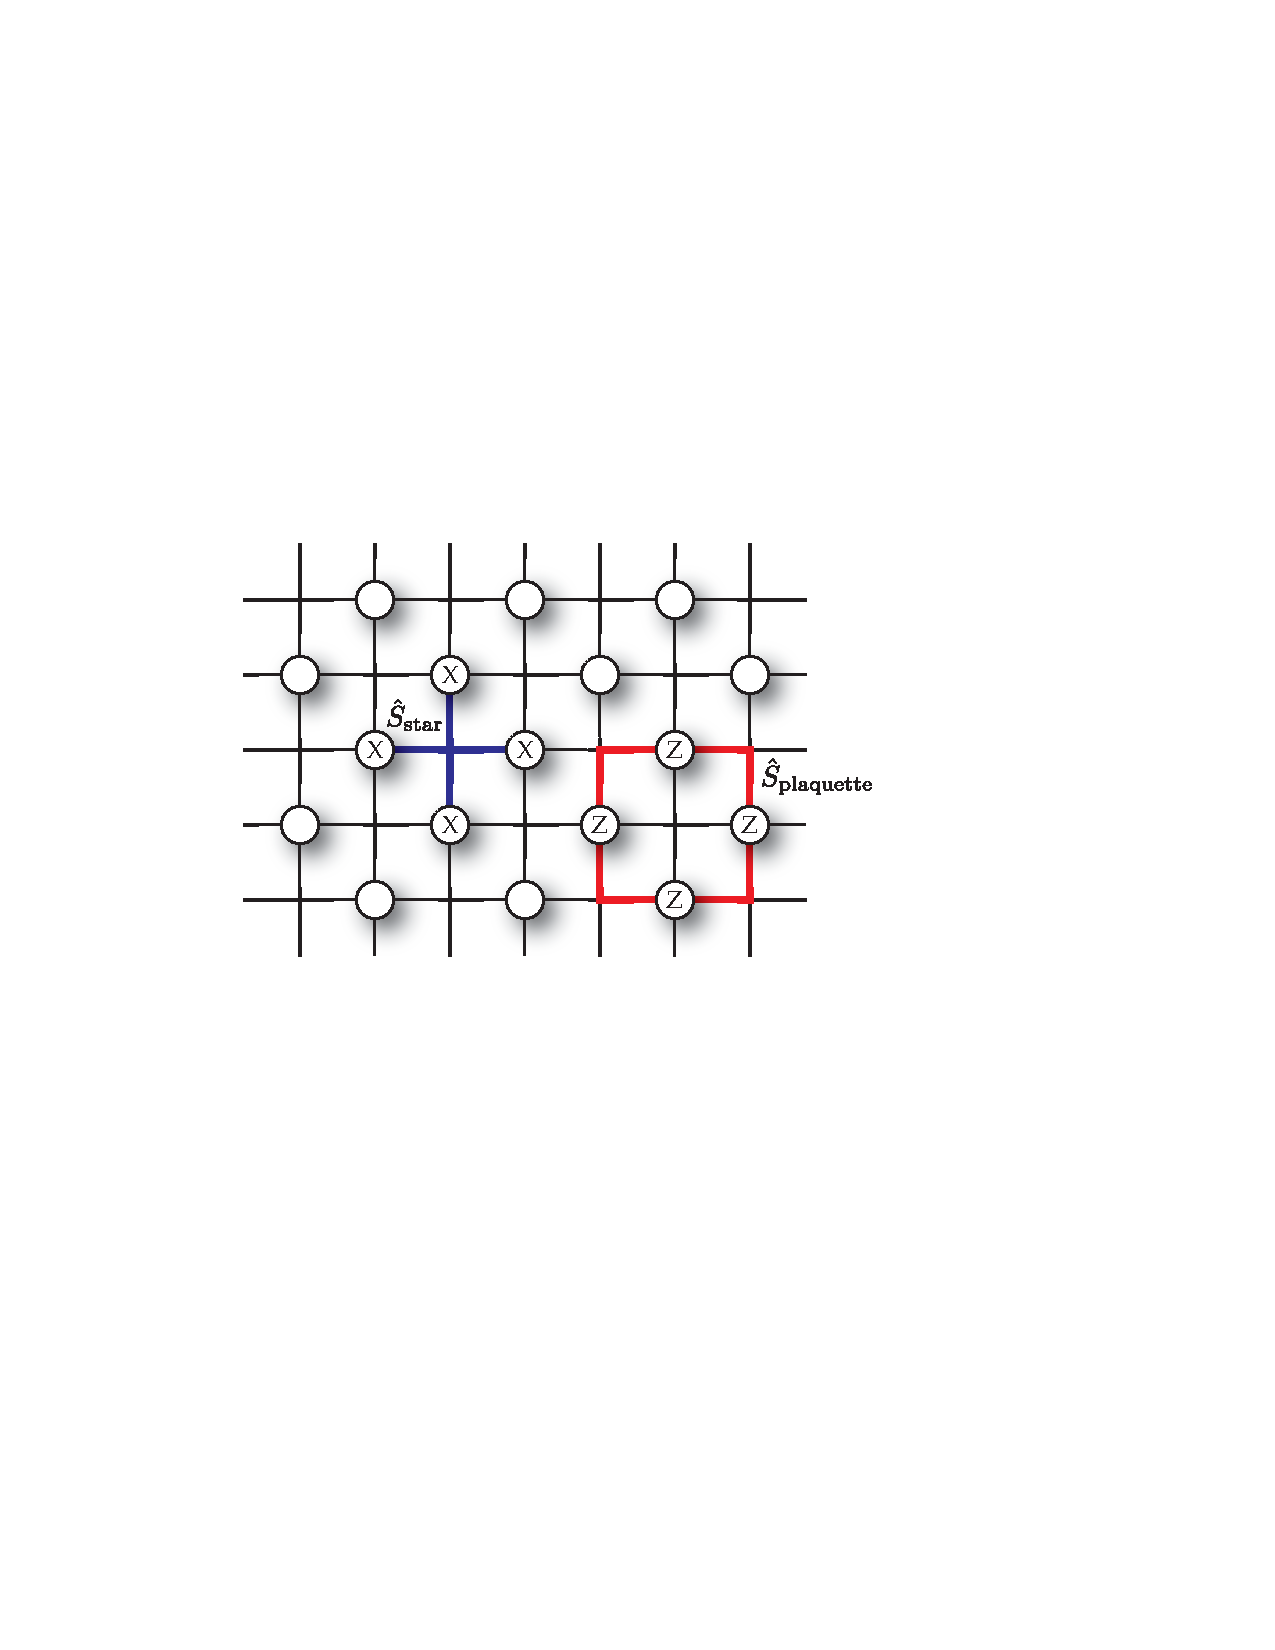
\includegraphics[width=\columnwidth]{toric_code}
	\caption{Graph representation of the toric QEC code, and its associated stabilisers. The star and plaquette stabilisers across all vertices, jointly specify the state of the graph up to two missing degrees of freedom, which encode a single logical qubit. Thus, a logical qubit is encoded jointly across the entire graph, not at any specific vertex. Logical operations are performed via operations following topological paths through the lattice (not shown). The graph may be distributed across multiple hosts for distributed quantum computation.} \label{fig:toric_code}
\end{figure}

\comment{How to convert cluster states to topological codes. Add discussion of how to perform gates.}

Having defined the toric code as such, QEC proceeds in a similar manner to any other stabiliser code -- we measure all the stabilisers, yielding a syndrome, from which we can determine geometrically where errors took place in the graph, which can subsequently be corrected (if below threshold).

The simplest example of error detection is the scenario where a single bit-flip ($\hat{X})$ error has occurred in the graph. Now exactly two plaquette stabilisers will yield the $-1$ measurement outcome, instead of the expected $+1$ outcome. These two stabilisers will necessarily be neighbouring ones, overlapping at the qubit where the error took place. Thus, using this geometric property, we are able to identify the location of the single $\hat{X}$ error and subsequently correct it. On the other hand, if there were too many errors, it is possible they could conspire against us to create ambiguity in the geometric argument for the location of the errors. \comment{Figure for both examples of this -- under and over threshold!}

Importantly, the stabilisers are all defined over geometrically localised neighbourhood regions, and do not require long-range measurements, making this type of code suitable to distributed models for quantum computation.

\comment{What about the actual computation? Can this still be distributed when we do the topological gates etc?}

%
% Classical Networking Protocols
%

\section{Classical networking protocols} \label{sec:classical_nets} \index{Classical networking protocols}

To set the context for our upcoming treatment of quantum networks, we begin by discussing \textit{classical} networks, and some of the key protocols behind their operation.

There have been numerous approaches employed in the past for sharing communications links between multiple users\index{Shared communication channels}. This includes:
\begin{itemize}
	\item Channel-switching: an entire communications channel is designated for exclusive use by a given user. \index{Channel switching}
	\item Packet-switching: data is divided into packets, which are routed independently by the network, being reconstructed by the recipient once all packets have been received.\index{Packet-switching}
	\item Time- or frequency-multiplexing: each user is designated a particular frequency spectrum or series of time-slots exclusively for their use. \index{Time-multiplexing}\index{Frequency-multiplexing}
	\item Code Division Multiple Access (CDMA): all users can broadcast over a channel simultaneously, and the construction of the coding technique enables demultiplexing of the distinct signals, despite their interference with one another.\index{Code Division Multiple Access (CDMA)}
	\item Ethernet: all users are free to broadcast over a shared channel at will, and \textit{collision detection} identifies when packets interfere, after which they are discarded and rebroadcast following a random waiting period, repeating until success.\index{Ethernet}
\end{itemize}

Nowadays packet-switched networks have become the norm in most digital networks, as they facilitate far greater efficiency in the use of network bandwidth, and are more easily scaled to greater numbers of users in a dynamic and ad hoc manner. It is foreseeable the same trend will continue with quantum technologies, especially given their initial high cost, where maximising network utility is paramount.

In this work we will focus on packet-switched networks when we later introduce our quantum networking protocols. However, with sufficient flexibility in the design of our upcoming quantum protocols, packet-switched networks can easily be made to effectively implement channel-switched, or time-/frequency-multiplexed communication.

%
% TCP/IP
%

\subsection{TCP/IP} \index{Transmission Control Protocol/Internet Protocol (TCP/IP)}

The present-day internet is built on top of a protocol stack comprising primarily the Internet Protocol (IP), User Datagram Protocol (UDP), and Transmission Control Protocol (TCP). Most commonly, these are simply referred to as TCP/IP. These define a stack of different layers of abstraction for communicating data packets between nodes in a network, determining their routing, and enforcing any quality of service requirements.

%
% Internet Protocol (IP)
%

\subsubsection{Internet Protocol (IP)} \index{Internet Protocol (IP)}

IP is the standard protocol employed in the internet for P2P communication of data packets. It is a low-level protocol that encapsulates digital data into packets containing a header field, which specifies routing information, most notably the IP addresses of the source and destination. IP does not enforce any kind of quality control, which is instead delegated to higher-level protocols like TCP (Sec.~\ref{sec:TCP}), a higher-level of abstraction built on top of IP (Sec.~\ref{sec:TCP}).

Multiple packets with the same source and destination needn't follow the same route -- the routing is determined dynamically in realtime by routers, based on network characteristics such as load or latency. Thus, packets belonging to the same underlying data may arrive out of order, or some may go missing altogether. IP does not address these issues, instead engaging in only `best-effort' delivery. 

In IP there is no central authority with knowledge of the state of the entire network, which tells routers in the network how to best route packets. Thus, IP must be complemented with up-to-date routing tables, held by routers/nodes in the network, which make routing decisions on a per-packet basis. This is achieved using gateway protocols, discussed next.

%
% User Datagram Protocol (UDP)
%

\subsubsection{User Datagram Protocol (UDP)} \index{User Datagram Protocol (UDP)}

The UDP is a simple protocol built on top of IP, based on a `send-and-forget' principle for sending data packets. That is, there is no quality of service guarantee, and no notifications are provided to the sender as to whether packets successfully reached their destination. However, a checksum (hash) forms a part of the packet headers to enable error detection by the recipient. The lack of quality control bypasses the associated latency, making it particularly useful in time-critical applications, where the late arrival of a packet is useless and therefore needn't be retransmitted.

UDP is connectionless, meaning that no designated connection is established between hosts. Instead data is simply transmitted and then forgotten about. The receiver may not even be operational on the network, in which case the packets are lost without notice.

Key examples for the use of UDP are realtime audio and video transmission. If a packet associated with a frame in a video link is delayed and arrives several frames late, it is useless, since it is associated strictly with a previous frame in the video that has already passed. Quality control, in the form of contacting the sender to request a retransmission, would therefore achieve nothing. This applies similarly to live audio streaming, such as voice-over-IP (VoIP), where the late arrival of a packet cannot possibly be correctly inserted into the audio playback and might as well be discarded.

Therefore, UDP prioritises latency over reliability, and is best suited to time-critical applications where quality of service is not relevant.

%
% Transmission Control Protocol (TCP)
%

\subsubsection{Transmission Control Protocol (TCP)} \label{sec:TCP} \index{Transmission Control Protocol (TCP)}

TCP differs from UDP in that it intrinsically supports quality control. The protocol is able to determine whether a packet successfully reached its destination, and if not, retransmit it as often as necessary to guarantee packet delivery. A checksum is also included in packet headers to enable error detection. This quality control has made TCP the dominant protocol employed in the present-day internet, where, in most scenarios, we wish to guarantee that data has been correctly delivered -- if an email is missing random segments of its text, users will become irate very quickly!

TCP is connection-oriented, meaning that a handshaking protocol establishes a dedicated bidirectional channel between two hosts. It also enforces packet reordering, to counter out-of-order packet arrival.

However, the enforced quality control and handshaking protocols incur a network performance overhead that UDP does not, since handshaking protocols consume bandwidth. Thus, TCP should not be used instead of UDP if there are no quality of service requirements.

%
% Ethernet
%

\subsection{Ethernet} \index{Ethernet}

Ethernet is a networking protocol based on `broadcasting' on a shared network. This model is particularly suited to local area networks (LANs), where all users share a single communications channel rather than dedicated P2P links, as shown in Fig.~\ref{fig:ethernet}.

\begin{figure}[!htb]
	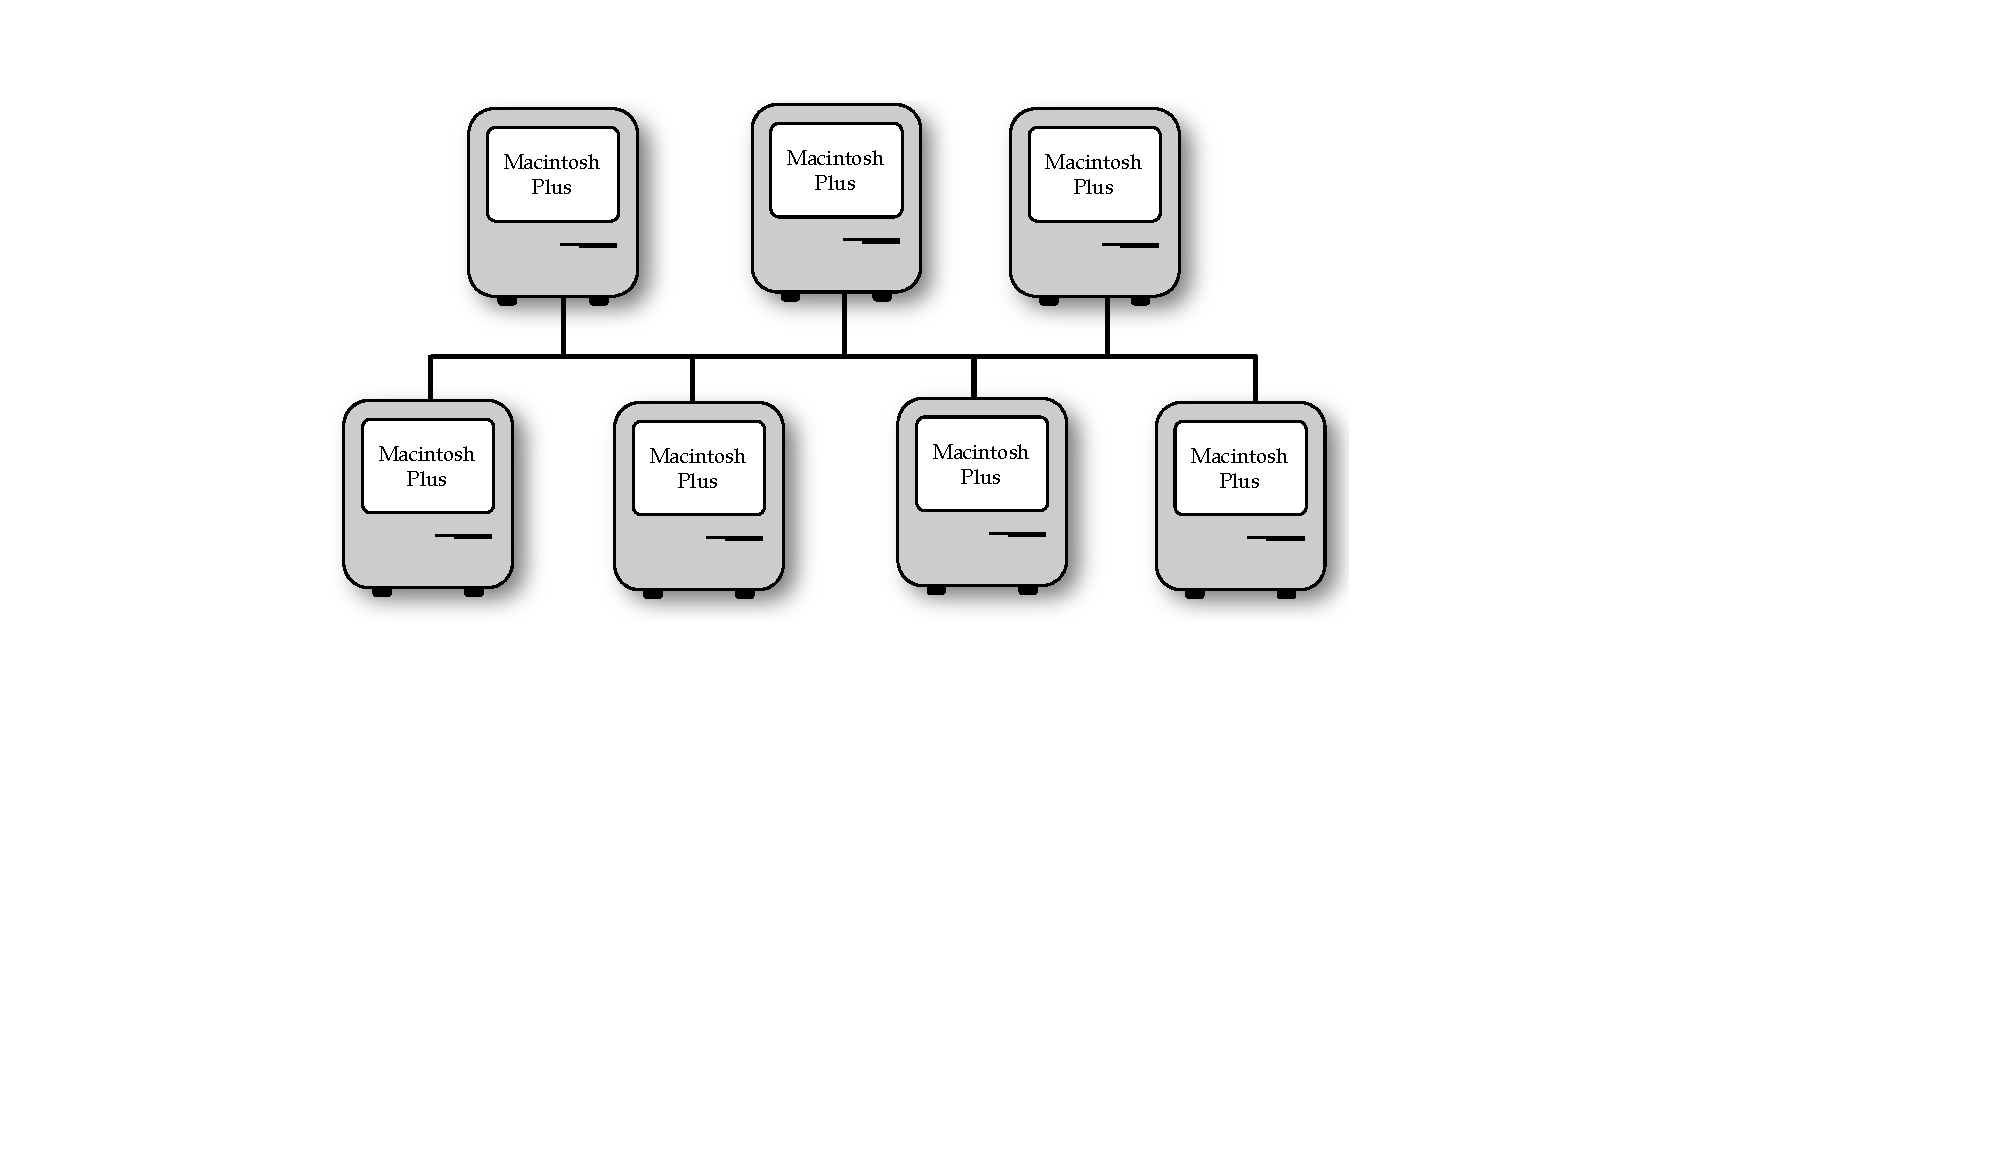
\includegraphics[width=\columnwidth]{ethernet}
	\caption{The topology of an Ethernet network, whereby all users share a common channel, which they can broadcast to at their leisure. If data packets collide, it is detected via the packets' checksums, and the corrupted packets may be re-broadcast after a random `backoff' waiting period, repeating this process until packet delivery is successful. Obviously the chance of collisions occurring increases with the number of connected users, thus network performance is inversely related to the number of nodes.} \label{fig:ethernet}
\end{figure}

In the Ethernet protocol, every user is free to broadcast data onto the shared channel as they please -- all users transmit to, and receive from a single shared channel. However, clearly sometimes packet `collisions' will occur\index{Collision handling}, resulting in packet corruption. To overcome this, Ethernet packets contain a checksum that can be used to verify upon arrival whether a packet has been corrupted by a collision. If a collision is detected, the respective users are able to re-broadcast, following a randomly chosen waiting period (known as `backoff')\index{Backoff}. Collisions therefore reduce network performance, and it follows that network bandwidth decreases with the number of users competing for bandwidth\footnote{Think of that awkward dinner table conversation, where two people start talking simultaneously. It's immediately obvious to them both that they are interfering with one another, and if they were to just talk over one another (packet collision), no one would understand either of them. So, they both awkwardly pause, before starting to speak again. In a \textit{really} awkward conversation, they will both start again simultaneously, after which there will be an even longer awkward pause before recommencing. Eventually, this self-regulating system will resolve itself probabilistically, with a sole victor controlling the airwaves, commanding the attention of the listeners. Provided that all dinner guests adhere to social etiquette and backoff appropriately, with repeated conversations, all guests will statistically receive an equitable share of attention, albeit with some wastage of conversation time owing to the periods of silence. Clearly, the proportion of the time wasted due to collisions will scale up with the number of guests, limiting the protocol to not-too-large tables (or very quiet guests).}.

From this protocol, any given packet will eventually be successfully transmitted uncorrupted, collision-free, albeit with uncertain timing that grows with the number of competing users. For this reason, the Ethernet protocol is not ideal for time-critical applications requiring hard guarantees on network latency.

The beauty of this approach is that only a single channel is required for connecting all users. No dedicated P2P connections are required. As the number of users increases, the complexity of the network topology does not -- requiring only the addition of a node to the existing backbone. For small LANs this is clearly reasonably functional. However, as the size of networks increases, the rate at which packet collisions occur increases, resulting in a reduction in network bandwidth. Thus, the Ethernet protocol is ideally suited to small LANs, but is clearly not viable at a global level, where network competition is astronomical and the overhead from backoff would reduce network performance to a standstill, wasting most of the bandwidth.

Another elegant feature of the Ethernet protocol is that bandwidth allocation is self-regulating, with bandwidth fairly and equitably allocated between users, not prioritising any user over another. This applies even in completely ad hoc networks, with users joining and leaving the network willy nilly. Provided all users are correctly and honestly implementing the \textsc{Broadcast and Backoff} protocol, network bandwidth is allocated evenly amongst users, and no mediating, overriding central authority is needed to oversee network resource allocation. This allows Ethernet networks to be truly `plug-and-play'.

%
% Gateway Protocols & Routing Tables
%

\subsection{Gateway protocols \& routing tables} \label{sec:gateway} \index{Gateway protocols} \index{Routing tables}

In the absence of a central mediating authority, routing decisions must be made by individual nodes in the network, upon receipt of packets. For routers to make sensible routing decisions, they must have some idea of the overall structure and state of the network. This is achieved using gateway protocols, which communicate information about the state of the network on a nearest-neighbour basis. There are various gateway protocols in use, with the Exterior Gateway Protocol (EGP)\index{Exterior Gateway Protocol (EGP)} and Border Gateway Protocol (BGP)\index{Border Gateway Protocol (BGP)} being very common.

We let every node in the network have a routing table, initially empty, that will ultimately be populated with information on how to best route incoming packets further along the route to their destination.

To mitigate the need for a central authority, nodes engage in only nearest neighbour communication, sharing their routing tables with one another, to query about the distance metrics (Sec.~\ref{sec:costs}) associated with routes to different destinations. This communication is taking place regularly, and as nodes' routing tables become populated, updating in real-time, they will (hopefully) reach a steady-state. From these tables, single-source shortest path algorithms (Sec.~\ref{sec:single_source_sp}) can be applied by nodes to construct a complete picture of costs to every point in the network.

%
% Network Hierarchies
%

\subsection{Network hierarchies} \index{Network hierarchies}

The disadvantage of Ethernet's \textsc{Broadcast and Backoff} principle is that packets are often wasted -- whenever a collision occurs. Because there is no mediating central authority, packet collisions are a certainty in a heavily-utilised shared network, each time resulting in packet loss, and an associated reduction in usable network bandwidth.

To the other extreme, we could have dedicated P2P channels between every pair of users. Then there would be guaranteed no packet collisions, and therefore maximum bandwidth efficiency, but the network would be extremely costly, and plug-and-play extremely challenging.

To address this dilemma, the topology and subdivision of networks need to be carefully designed. If we consider a large organisation, for example, potentially networking thousands of desktop PCs, the bandwidth wastage associated with packet collisions could grind the entire network to a halt, were all thousands of PCs to be communicating large amounts of data simultaneously. However, if a hierarchy of subnetworks could be implemented, rather than a single monolithic network, efficiency could be improved drastically.

Suppose our hypothetical organisation had several different departments, and users had a tendency to communicate primarily with other users in the same department. By defining distinct departmental subnets, which individually implement Ethernet, but interconnect with one another using an alternate routing framework, we can easily see that many unnecessary packet collisions may be entirely avoided. That is, why broadcast data to users who we know don't want it? A simple example of this is shown in Fig.~\ref{fig:net_hierarchy}.

\begin{figure}[!htb]
	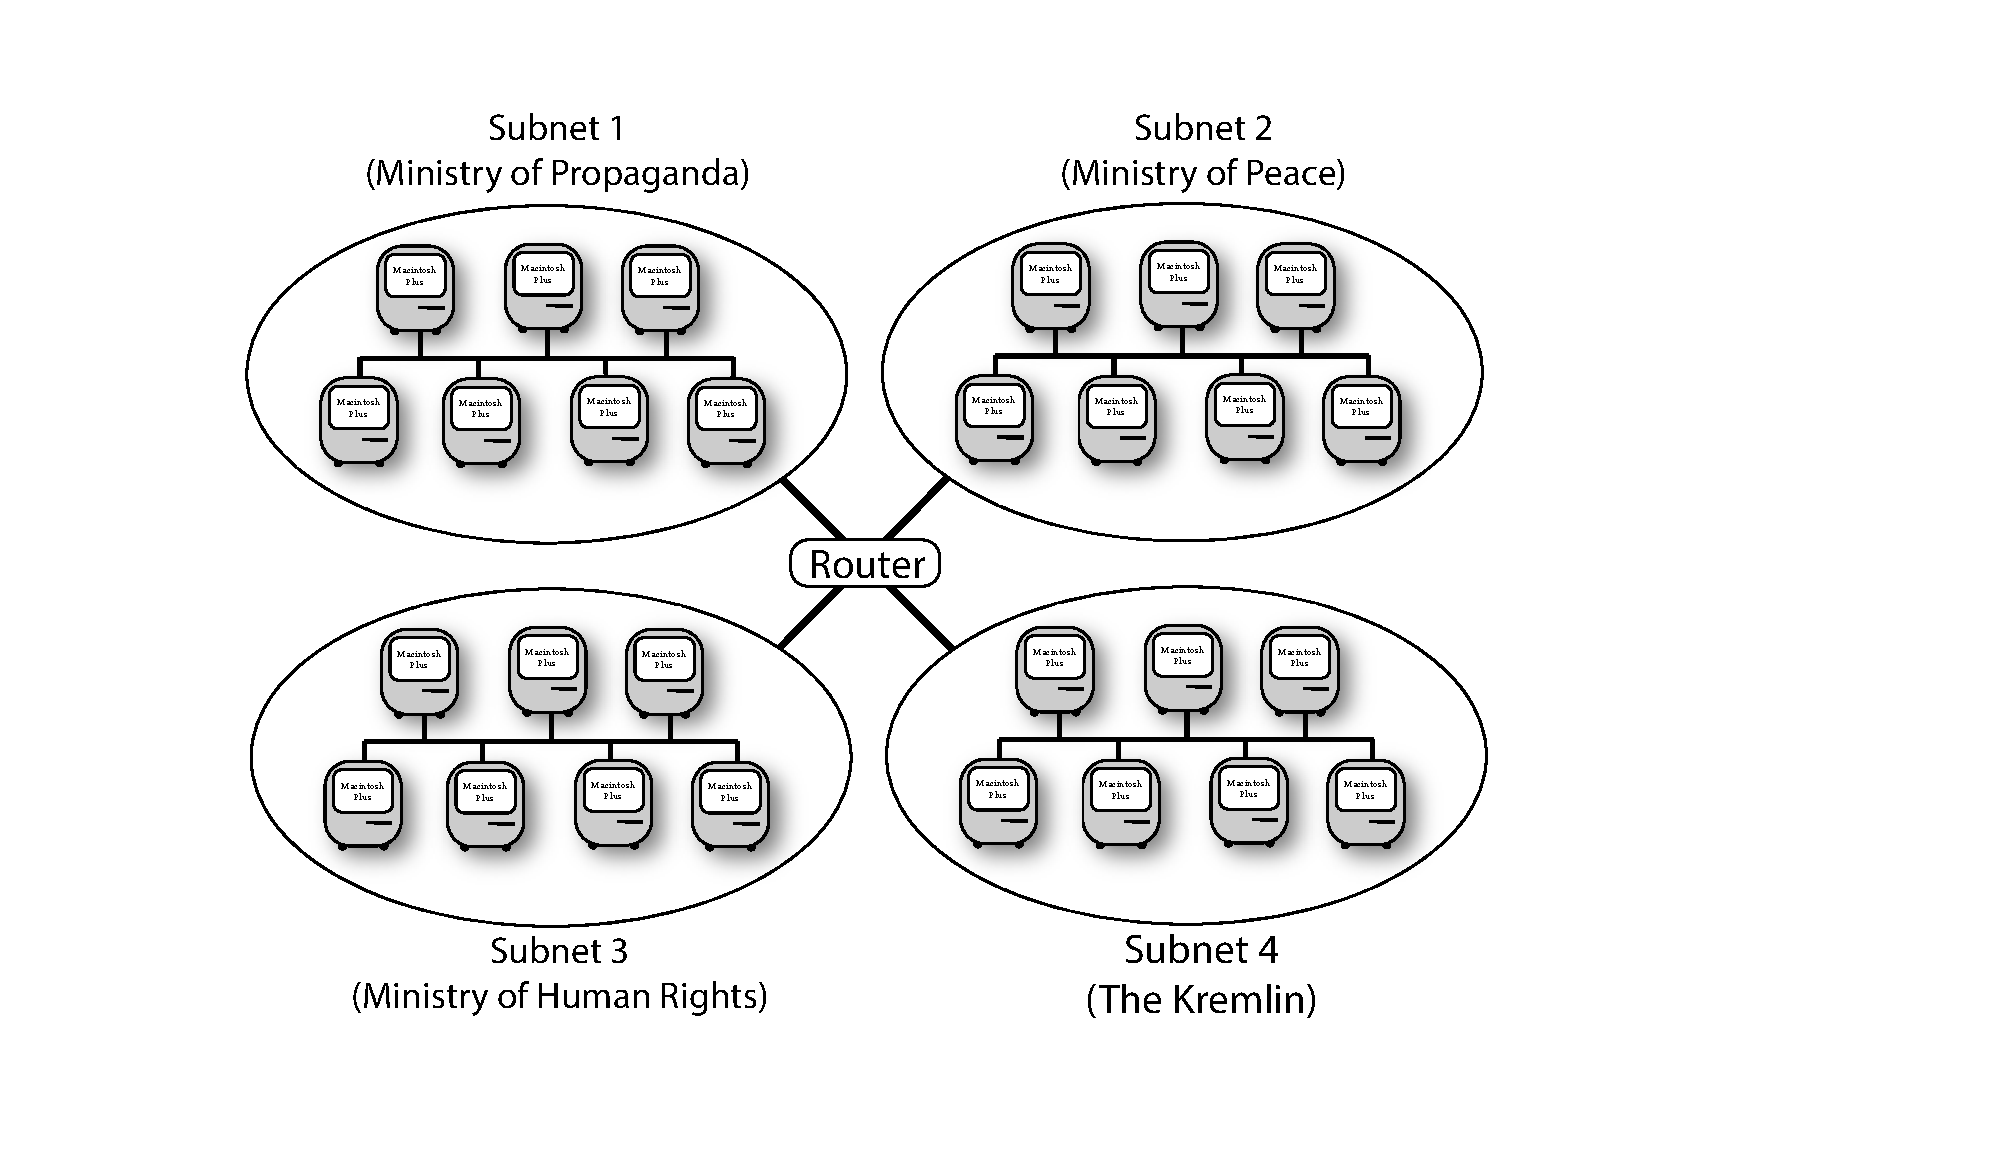
\includegraphics[width=\columnwidth]{network_hierarchy}
	\caption{Simple example of a network with two levels in its hierarchy. At the lowest level are 4 different subnets belonging to different departments within an organisation, each of which implements Ethernet networking. Above this, the subnets connect together in a star network via a central router. By subdividing the network hierarchy as such, if most traffic emanating within a subnet stays within that same subnet, collisions between packets on different subnets are avoided, thereby improving the efficiency of the subnets' Ethernet implementations.} \label{fig:net_hierarchy}
\end{figure}

Extending upon this simple intuitive example, enormous amounts of research and development have been invested into the design of network hierarchies, and how to optimise their efficiency. A pressing consideration in the design of network protocol stacks is therefore to accommodate for multiple routing protocols, and enabling their intercompatibility.

%
% Mathematical Representation of Networks
%

\section{Mathematical representation of networks}

We now turn our attention to defining a mathematical construction for the representation of (quantum and/or classical) networks, that we will subsequently rely on heavily in our framework for quantum networks. This encompasses representing networks as graphs, representing the cost of communications within the network, and how to optimise network routing to minimise costs.  These notions will be essential in our treatment of quantum networks.

%
% Graph-Theoretic Representation
%

\subsection{Graph-theoretic representation} \index{Network graphs}

We consider a classical network to be a weighted, directed graph,
\begin{align}\index{Network graph}
	G=(V,E),
\end{align}
where vertices represent \textit{nodes} (\mbox{$v\in V$}) in the network, and the weighted edges represent communication \textit{links} (\mbox{$e\in E$}) between neighbouring nodes \cite{???}.

A node could be, for example, data storage, a classical computer implementing a computation, a router that switches the connections between incoming and outgoing links, or an end-user -- anything that communicates with the network, sender or receiver. A link on the other hand is any arbitrary means of communication between nodes, such as optical fibre, satellite, radio, electrical, smoke signals, tin cans connected by a taut piece of string, or well-trained carrier pigeon. In the protocols to be described here, it is completely irrelevant what the specific mediums for communication are. Rather what matters are \textit{costs} and \textit{attributes}, quantifying the relative performance of different links.

A key feature of the global internet is redundancy. In a packet-switched environment, sending identical packets twice might each follow entirely different routes to their common destination. Node-to-node redundancy is easily accommodated for in the graph-theoretic model by allowing multiple distinct edges between nodes. It is extremely important to accommodate multiple edges in network graphs, since redundant routes provide a direct means by which to load-balance a route. So, for example, a hub in Australia might connect to a sister hub in New Zealand using both a fibre-optic undersea cable, and simultaneously via a satellite uplink. If the faster of the two connections is running out of capacity, a proportion of the packets can simply be switched to the other link, thereby balancing the load. For this reason we abstain from using an adjacency matrix representation for network graphs, as they do not accommodate redundancy.

%
% Network Costs & Attributes
%

\subsection{Network costs \& attributes} \label{sec:costs} \index{Costs}\index{Attributes}

The edge weights in $G$ represent the \textit{costs} ($\vec c$) and \textit{attributes} ($\vec a$) associated with using that link. In general these needn't be single numbers, but would rather be sets, representing different types of costs and attributes of links, of which there may be many. These could include, for example, latency, bandwidth, dollar cost, and quality.

The distinction between costs and attributes, is that costs may be expressed in terms of units which may be interpreted as distances metrics in a Euclidean sense, obeying the following requirements:

\begin{definition}[Network cost metrics] \label{def:metric} Cost metrics satisfy the properties:\index{Network cost metrics}
	\begin{itemize}
    	\item Identity operations: If a channel performs nothing, its associated cost is zero, \mbox{$c(\mathbb{\hat{I}}) = 0$}.
    	\item Triangle inequality: \\ $c(v_1\to v_2\to v_3) \leq c(v_1\to v_2) + c(v_2\to v_3)$, \\ across all paths \mbox{$v_1 \to v_2 \to v_3$}.
    	\item Positivity: \mbox{$c\geq 0$}. This ensures that shortest-path algorithms will function correctly.
	\end{itemize}
\end{definition}
Attributes, on the other hand do not have a distance interpretation, and may have arbitrary structure. A detailed discussion on the relationship between costs and attributes is presented in Sec.~\ref{sec:c_vs_a}.

The reason we demand costs have a distance interpretation is so that graph-theoretic pathfinding algorithms (Sec.~\ref{sec:shortest_path}) are applicable, allowing us to build upon the vast pre-existing understanding of graph theory. Ideally we would like equality in costs' triangle inequality, which yields an exact cost. But often this isn't possible and we are satisfied with the inequality, which simply dictates an upper bound on cost.

A detailed discussion of some of the major costs and attributes that realistic quantum networks will be subject to is presented in Sec.~\ref{sec:quantum_meas_cost}.

A \textit{route}\index{Routes} between two nodes, Alice ($A$) and Bob ($B$), of the network, $G$, is an acyclic subgraph connecting those nodes, \mbox{$R_{A\to B}\subseteq G$}. In general ad hoc networks there will typically be multiple paths between two nodes \mbox{$A\to B$}. For a particular cost metric, the cost of an entire route is simply the sum of the costs of each of the constituent links,
\begin{definition}[Route costs]
The net cost of a route \mbox{$A\to B$}, traversing nodes $v_i$, is,
\begin{align}\index{Route costs}
c(R_{A\to B}) = \sum_{i=1}^{|R_{A\to B}|-1} c(v_i \to v_{i+1}),
\end{align}
where $v_i$ is the $i$th node in the route $R_{A\to B}$.
\end{definition}

Fig.~\ref{fig:example_routes} illustrates a simple example network with all of its available routes, \mbox{$R_{A\to B} \subseteq G$}. Fig.~\ref{fig:simp_route_opt} illustrates the optimal path for \mbox{$A\to B$} based on edge weights.

\begin{figure}[!htb]
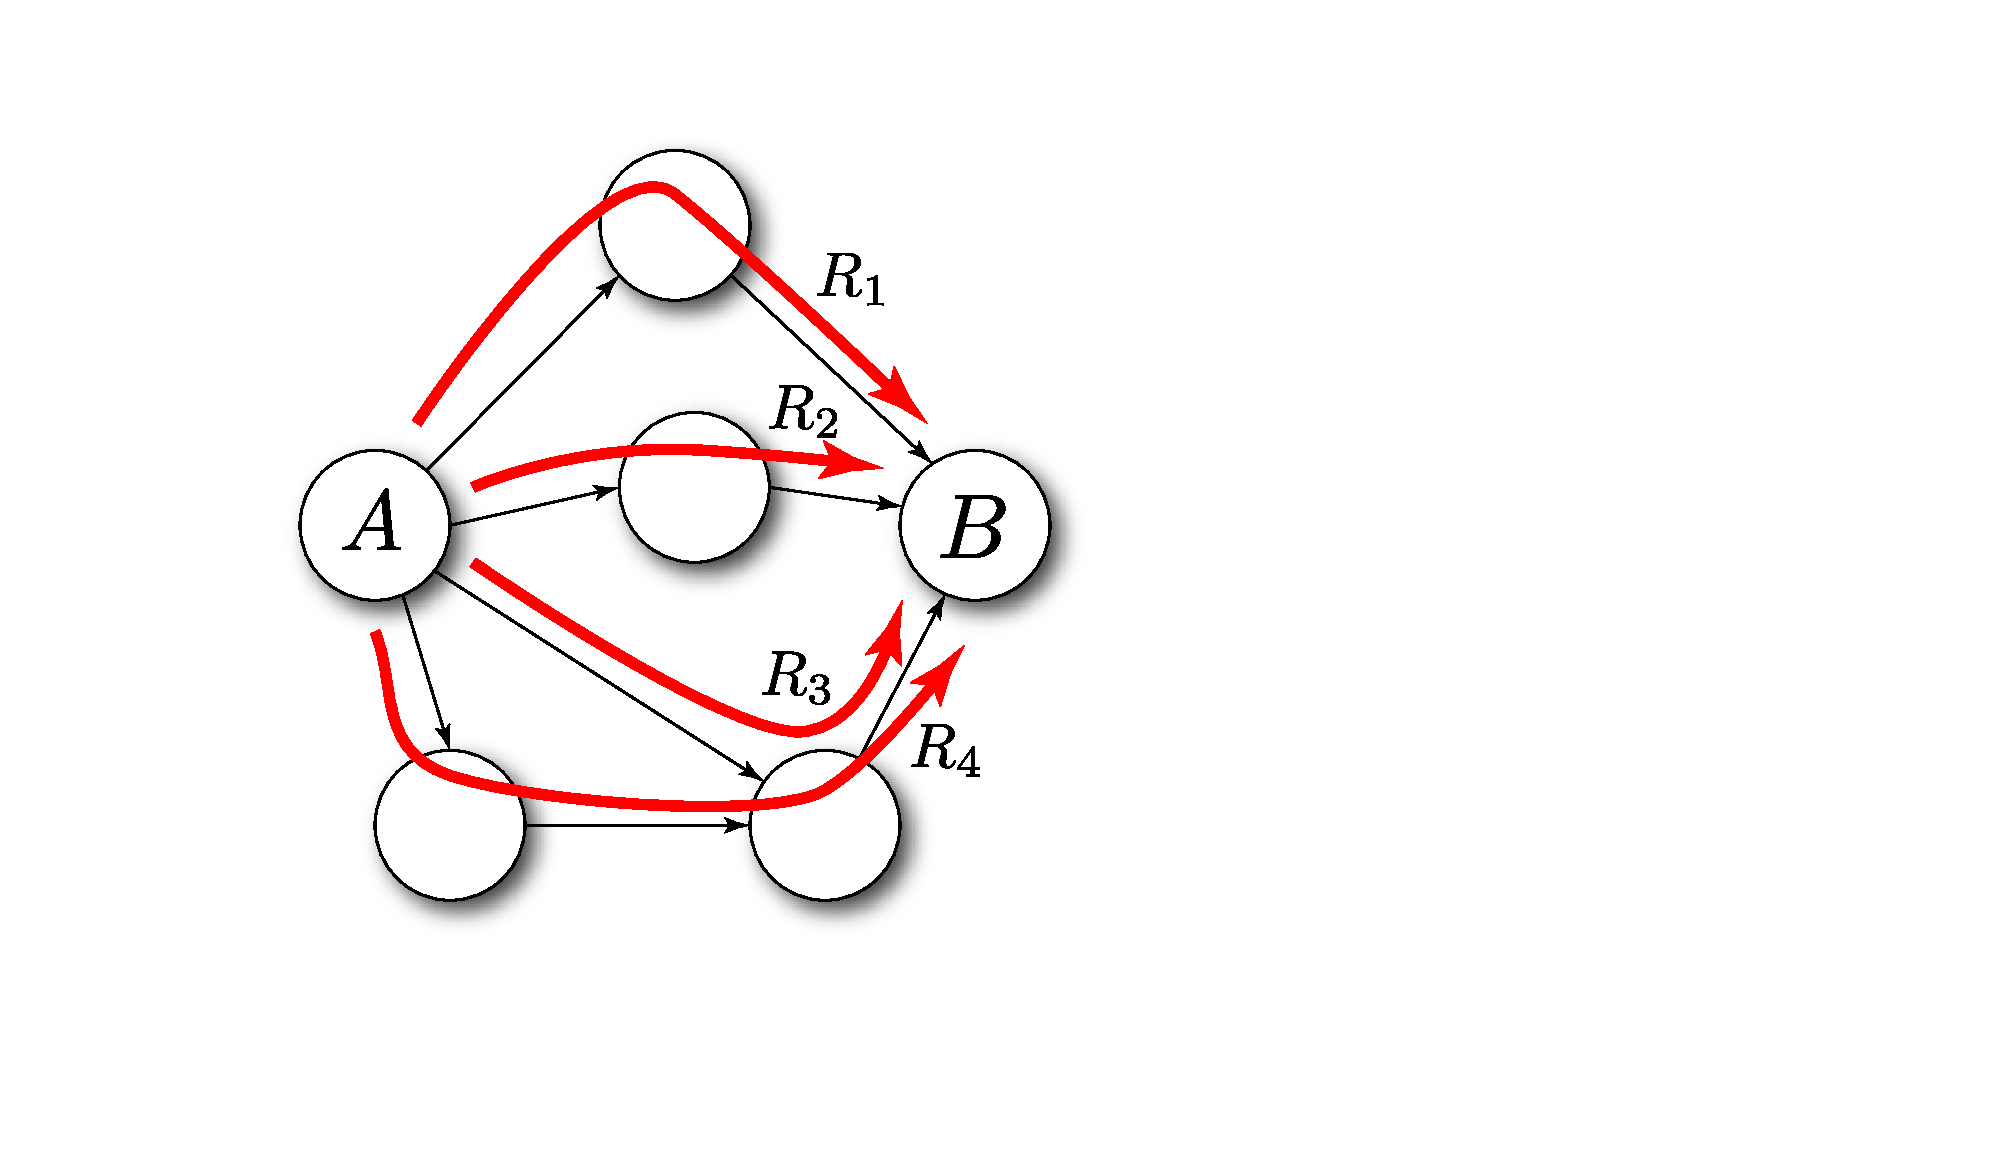
\includegraphics[width=0.65\columnwidth]{example_routes}
\caption{Example of a simple network with multiple routes \mbox{$A\to B$}. Note that $R_3$ and $R_4$ are competing with one another for use of the last link, which the routing strategy, $\mathcal{S}$, will need to resolve if multiple simultaneous transmissions are taking place.} \label{fig:example_routes}
\end{figure}

\begin{figure}[!htb]
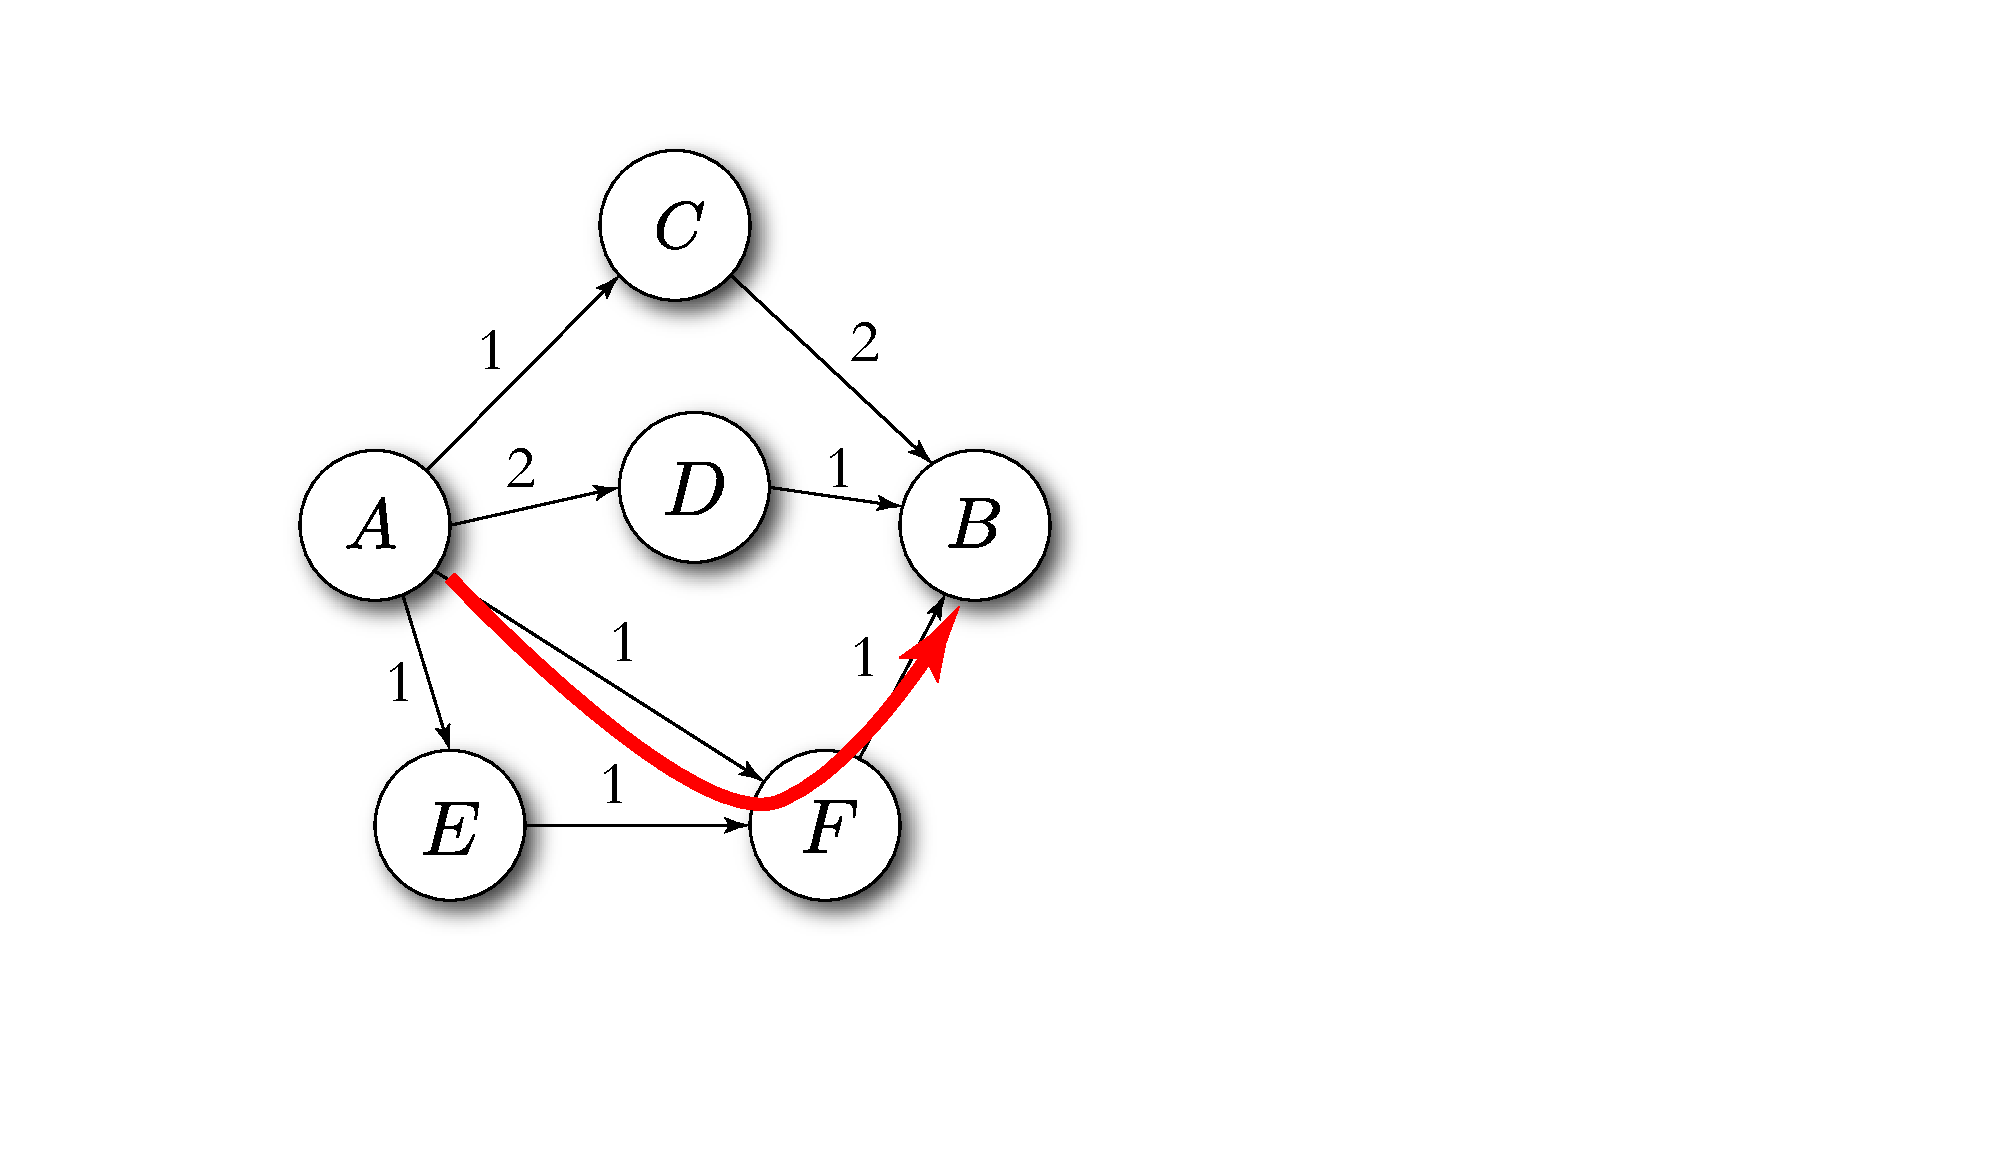
\includegraphics[width=0.6\columnwidth]{example_opt}
\caption{The same network graph from Fig.~\ref{fig:example_routes}, with links weighted by some arbitrary cost metric. Applying a shortest-path algorithm yields the optimal route between Alice and Bob to be \mbox{$A\to F\to B$}, which incurs a net cost of \mbox{$c=2$}, as opposed to all other routes, which incur a net cost of \mbox{$c=3$}.} \label{fig:simp_route_opt}
\end{figure}

In a given network, it is unlikely that only a single cost metric or attribute will be of interest when determining optimal routings. There may be a tradeoff between different measures. For example, for time-critical applications the cost of a route might be considered a combination of both dollar cost and latency -- a satellite has very low latency but is extremely expensive, while a carrier pigeon is slow but cheap (and prohibited by PETA). What is the best tradeoff between the two?

To accommodate this, we allow the \textit{net cost} of a route to be defined as an arbitrary function of other primitive cost metrics and attributes of the route,
\begin{definition}[Net cost]
The net cost of a route \mbox{$A\to B$} is given by,
\begin{align} \label{eq:net_cost_R} \index{Net cost}
c_\text{net}(R) = f_\text{cost}(\vec{c}(R),\vec{a}(R)),
\end{align}
where $c_\text{net}$ is a single numeric value representing the net cost as calculated from an arbitrary cost function $f_\text{cost}$.
\end{definition}
Note that the net cost needn't be a metric, as the cost function could be arbitrary. The net cost can be thought of as a ranking for routes, but not necessarily as a metric that accumulates across routes.

Eq.~(\ref{eq:net_cost_R}) gives us the net cost of a given route. For multiple users we would like to simultaneously optimise the cost across all users of the network. Thus we define the routing cost for the entire network to be,
\begin{definition}[Network routing cost]
	The net routing cost of all costs, over all active routes $\vec{R}$ is,
\begin{align} \label{eq:c_total}
c_\text{total}(\vec{R}_{\vec{A}\to \vec{B}}) = \sum_{r \in {\vec R}_{\vec{A}\to \vec{B}}} c_\text{net}(r),
\end{align}
where $\vec{R}_{\vec{A}\to \vec{B}}$ is a set of routes connecting each pair \mbox{$A_i\to B_i~\forall ~ i$}.
\end{definition}

%
% Flow Networks
%

\subsection{Flow networks} \label{sec:flow_networks} \index{Flow networks}

On a shared network with many users utilising the network simultaneously, it may be the case that the preferred goal for the network is to maximise \textit{flow} \cite{???} -- the total amount of information that can be transmitted per unit time, i.e the net utilisation of the network's resources, summed over all users. In this case we can build on the existing theory of \textit{flow networks} \cite{???}, which characterise the load of links within the network.

A flow network is easily obtained from the network graph by associating a `capacity' attribute with each link and defining the graph weighted by the capacities as the flow network, preserving the underlying structure of the network graph.

When a route within the graph is utilised, we decrement the capacities of each link in that route, generating the so-called \textit{residual network} \cite{???}, which will now take the place of the original network in subsequent calculations. This process effectively tallies the links' utilisation, and when the tally hits zero, the link can no longer be used for any new routes. This forms a basic building block for more complex flow network algorithms.

There are many variations on flow networks. The simplest case is of a single user transmitting multiple packets simultaneously to a recipient. Depending on link capacities, different packets may need to follow different routes through the network, if network performance is to be maximised. Alternately, it may not be possible to send the desired number of packets simultaneously if the network capacity saturates.

The more complex (and realistic) scenario is of multiple users each transmitting from distinct starting nodes to distinct recipient nodes across a shared network. This is known as a \textit{multi-commodity flow network} \cite{???}, and is likely to be the dominant class of networks in real-world networking applications.

%
% Routing Strategies
%

\subsection{Routing strategies} \label{sec:route_strats} \index{Routing strategies}

A \textit{strategy}, $\mathcal{S}$, is simply an algorithm that chooses a route ($k$), based on the starting ($i$) and finishing ($j$) nodes of a communication, and also updates the vectors of costs and attributes within the network associated with the utilisation of that route,
\begin{definition}[Routing strategies]
A routing strategy is defined by,
	\begin{align}
\mathcal{S}(i,j,\vec{c},\vec{a}) &\to \{k,{\vec{c}}~',{\vec{a}}~'\}, \nonumber \\
i,j &\in V, \nonumber\\
k &\in \{R_{v_i\to v_j}\},
\end{align}
\end{definition}
with the goal of minimising a chosen cost measure.

No particular route through a network is going to have infinite capacity, and therefore we cannot typically always reemploy the same most cost-effective route for all data. Particularly in multi-user networks, as routes are employed for communicating quantum states, their cost metrics may change according to load, or other external influences. For this reason, it is important that strategies accommodate dynamic changes in the network. This is easily accounted for by letting the edge weights in our network graph be a function of time, $G_t$, which are updated via the application of a strategy, which may also be a function of time,
\comment{Add to def}
\begin{align} \label{eq:S_G}
G_{t+1} = \mathcal{S}_t(G_t).
\end{align}
For example, the network might have bandwidth restrictions on some links, in which case if more than a certain amount of data is transmitted through a link, it is no longer available for use until previous transmissions have completed. Or, based on market dynamics, the dollar cost of utilising a link may change with its demand.

This type of cost minimisation approach to routing is analogous to \textit{distance-vector routing protocols} in classical networking theory.

A detailed exposition of routing strategies is provided in Sec.~\ref{sec:strategies}.

%
% Strategy Optimisation
%

\subsection{Strategy optimisation} \label{sec:strat_opt} \index{Strategy optimisation} 

Clearly the goal when choosing routing strategies is to minimise the total cost, Eq.~(\ref{eq:net_cost_R}). That is, solving the optimisation problem,
\begin{definition}[Strategy optimisation]
The optimisation of strategies with a network comprising net costs $c_\text{total}$ is given by,
\begin{align}
c_\text{min} &= \underset{\mathcal{S}}{\text{min}}(c_\text{total}), \nonumber \\
\mathcal{S}_\text{opt} &= \underset{\mathcal{S}}{\text{argmin}} (c_\text{total}).
\end{align}
\end{definition}

Choosing optimal strategies is a challenging problem, potentially requiring complex, computationally inefficient optimisation techniques. Strategy optimisation is an example of resource allocation, whose optimal solutions are often notoriously difficult to solve exactly, residing in complexity classes like \textbf{NP}-complete\index{\textbf{NP} \& \textbf{NP}-complete} (or worse!). In general, the number of possible routes through a graph will grow exponentially with the number of vertices. Thus, explicitly enumerating each possible route is generally prohibitive for large networks, unless some known structure provides `shortcuts' to optimisation. Having said this, Dijkstra's shortest path algorithm (discussed in Sec.~\ref{sec:shortest_path}) is the perfect counterexample, demonstrating that although an exponential number of routes may exist between two points, an optimal one can be found in \textbf{P}.

%
% Ad hoc Operation vs. Central Authorities
%

\subsubsection{Ad hoc operation vs. central authorities} \index{Central authorities} \index{Ad hoc networks}

When considering strategy optimisation, the first question to ask is `Who performs the optimisation, and who has access to what information?'.

In terms of who performs the optimisation, the two main options are that either each node is responsible for optimising the routes of packets passing through it (\textsc{Individual} algorithms), or there is a reliable and trusted central authority who oversees network operation and performs all strategy decision-making (\textsc{Central} algorithms).

In the case of \textsc{Individual} algorithms, the required knowledge of the state of the network could be obtained using network exploration algorithms (Sec.~\ref{sec:path_exp}) or gateway protocols (Sec.~\ref{sec:gateway}). 

On the other hand, for \textsc{Central} algorithms, either network exploration could be employed, or alternately the network policy could require nodes to notify the central authority upon joining or leaving the network. The former introduces an overhead in classical networking resource usage, since network exploration must be performed routinely to keep the ledger of nodes up-to-date. The latter, on the other hand, avoids this, but introduces a point of failure, in that all network participants must be reliable in notifying the central authority as required by the network policy. Failure to do so could result in invalid or suboptimal strategies.

%
% Local vs. Global Optimisation
%

\subsubsection{Local vs. global optimisation} \index{Local optimisation}\index{Global optimisation}

There are two general approaches one might consider when choosing strategies -- \textit{local optimisation} (\textsc{Local}) and \textit{global optimisation} (\textsc{Global}). \textsc{Local} simply takes each state to be communicated, one-by-one, and allows it to individually choose an optimal routing strategy based on the state of the network at that moment. \textsc{Global} is far more sophisticated and simultaneously optimises the sum of the routing costs, Eq.~(\ref{eq:c_total}), of all currently in-demand routes.

To implement \textsc{Local} optimisation, either \textsc{Individual} or \textsc{Central} algorithms may be employed. On the other hand, \textsc{Global} optimisation necessarily requires a \textsc{Central} algorithm, since it requires knowledge of the entire state of the network, which is collectively optimised.

Since \textsc{Global} represents the class of all algorithms that take all network costs by all packets into consideration, it must clearly perform at least as well as \textsc{Local}, which only takes into consideration the costs of a given packet. But we expect \textsc{Global} to perform better than \textsc{Local} in general, owing to the additional information it takes into consideration. We express this as \mbox{\textsc{Local}$\subset$\textsc{Global}}. However, \textsc{Global} requires solving a complex, simultaneous optimisation problem, which is likely to be computationally hard, whereas \textsc{Local} can be efficiently solved using multiple independent applications of, for example, an efficient shortest-path algorithm (so-called \textsc{Greedy} algorithms), discussed in Sec.~\ref{sec:shortest_path}.

A further stumbling block for \textsc{Global} is that it requires some central authority, responsible for the global decision-making, to have complete, real-time knowledge of the state of the entire network. This may be plausible for small LANs, but would clearly be completely implausible for the internet as a whole. So it is to be expected that different layers and subnets in the network hierarchy will employ entirely different strategy optimisation protocols. This is certainly reminiscent of the structure of the present-day internet.

Roughly speaking, we might intuitively guess that at lower levels in the network hierarchy, responsible for smaller subnets, there will be a tendency towards the adoption of \textsc{Global} strategies, as full knowledge of the state of the subnet is readily obtained and maintained. However, as we move to the highest levels of the network hierarchy (e.g routing of data across international or intercontinental boundaries), we might expect more laissez-faire (i.e \textsc{Greedy}) strategies to be adopted, since the prospects of enforcing a central authority with full knowledge of the state of the internet, who is also trusted by all nations to fairly and impartially allocate network resources and mediate traffic, is highly questionable.

We will not aim to comprehensively characterise the computational complexity of \textsc{Global} strategies. However, in Sec.~\ref{sec:strategies} we will present some elementary analyses of several toy models for realistic strategies. Some such strategies are efficient although not optimal, but nonetheless satisfy certain criteria we might expect.

Future developments in the optimisation techniques required for \textsc{Global} strategies may improve network performance, leaving our techniques qualitatively unchanged.

When employing \textsc{Local}, on the other hand, things are often far simpler. If we are optimising over a cost metric satisfying the distance interpretation, we may simply employ a shortest-path algorithm to find optimal routes through the network.

If one were to become even more sophisticated, one might even envisage treating network resource allocation in a game theoretic context \cite{???}, which we won't even begin to delve into here.

%
% Message- vs. Packet-Level Routing
%

\subsection{Message- vs. packet-level routing}

In Eq.~(\ref{eq:S_G}) we defined the action of a strategy, $\mathcal{S}$, on a network, $G$. However, we were intentionally ambiguous in our introduction of the time-dependence, given by $t$. This is to allow us to consider changes at one of two different time-scales: the packet level, or the message level. The \textit{message} is the entire data stream transmitted from Alice to Bob, whereas the \textit{packet} is a small block of data taken from the message, where each packet may be independently routed.

When defining the action of strategies, we could do so at either of these time-scales. We could choose routes in their entirety, from start to finish, at the beginning of the message transmission, under the assumption that the costs in the network will be constant over that duration and no one will misbehave. We refer to such strategies as \textit{message-level strategies}. Alternately, and perhaps more realistically in many scenarios, the costs and attributes of a network could be highly dynamic and readily change within the transmission time-window. In that case, we will employ \textit{packet-level strategies}, which reevaluate the strategy independently for each packet and for each of their hops between nodes.

In our future discussions on routing strategies, context will make it clear when we are referring to packet- or message-level strategies.

%
% Quantum Networks
%

\section{Quantum networks} \label{sec:quant_net} \index{Quantum networks}

Quantum networks comprise all the same ingredients as classical networks, but with additions. Nodes can additionally implement quantum computations, quantum-to-classical interfaces (i.e measurements), quantum-to-quantum interfaces, quantum memories, or any quantum process in general. The cost associated with links could include measures that are uniquely quantum, such as fidelity, purity or entanglement measures, none of which are applicable to classical digital data. As in the classical case, our goal is to find routing strategies that optimise a chosen cost measure. But in the quantum context costs will be constructed entirely differently owing to the quantum nature of the information being communicated.

We envisage a network with a set of senders, $\{A_i\}$, and receivers, $\{B_i\}$, residing on a time-dependent network graph, $G_t$, as before. $A$ have sets of quantum states to communicate, $\{\hat\rho_\text{data}(i)\}$. For each $\hat\rho_\text{data}(i)$ she must choose appropriate strategies $S_t$, such that the overall cost is optimised, for some appropriate cost measure. Compared to classical resources, equivalent quantum resources are costly and must be used efficiently, making resource allocation strategies of utmost importance.

The routing strategies we introduce in Sec.~\ref{sec:strategies} will not always guarantee that packets have immediate access to network bandwidth the moment they demand it. Inevitably, in shared networks there will sometimes be competition and congestion, forcing some users to wait their turn. For this reason, many quantum networks will require at least some nodes (the ones liable to competition) to have access to quantum memories, such that quantum packets can be stored for a sufficient duration that they can wait their turn on the shared network resources. The required lifetime of a quantum memory will then be related to overall network congestion. Of course, quantum memories induce quantum processes of their own, which need to be factored into cost calculations. Quantum memories are easily accommodated for in the QTCP framework by allowing self-loops at nodes, which implement a memory process. The implementation of quantum memory is discussed in Sec.~\ref{sec:memory}.

Given that classical networking is decades more advanced than quantum networking, and extremely cheap and reliable, we will assume that classical resources `come for free', and only quantum resources are of practical interest. That is, classical communication and computation is a free resource available to mediate the operation of the quantum network. We therefore envisage a \textit{dual network} with two complementary networks operating in parallel and in tandem -- the quantum network for communicating quantum data, and a topologically identical classical network operating side-by-side and synchronised with the quantum network.

The motivation for the dual network is to ensure that classical and quantum data that jointly represent packets (Sec.~\ref{sec:prot_stack}) remain synchronised and subject to the same QoS issues, such as packet collisions (Sec.~\ref{sec:collision}) and network congestion.

We envisage quantum networks to extend beyond just client/server quantum computation, to include the free trade of any quantum asset. This includes state preparation, measurement, computation, randomness, entanglement, and information. Much like the classical internet, by allowing quantum assets to be exchanged, we can maximise utility, improve economy of scale, and enable new models for commercialisation.\index{Quantum assets}

%
% Quantum Channels
%

\section{Quantum channels} \label{sec:quant_chan} \index{Quantum channels}

Like classical channels, quantum channels are inevitably subject to errors. These errors could be an intrinsic part of the system, or induced by interaction with the external environment. The \textit{quantum process} formalism provides an elegant mathematical description for all physically realistic error mechanisms \cite{bib:NielsenChuang00, bib:Gilchrist05}. Here we review the quantum process formalism and how it applies to quantum networks. This paves the way for the quantum notion of costs and attributes.

%
% Quantum Processes
%

\subsection{Quantum processes} \index{Quantum processes}

To quantify the operation of nodes and links within our network, we must characterise the evolution they impose upon quantum states passing through them. Quantum processes, also known as \textit{trace-preserving, completely positive maps} (CP-maps) are able to capture all the physical processes relevant to quantum networking, such as: unitary evolution; decoherence; measurement; quantum memory; state preparation; switching; and, indeed entire quantum computations. And they are able to capture physical processes in any degree of freedom, most commonly in the qubit basis, but also, for photons, in the spatio-temporal, photon-number, phase-space, or polarisation degrees of freedom.

Quantum processes are most easily represented using \textit{Kraus operators}, $\{\hat{K}_i\}$,
\begin{align} \label{eq:kraus_rep}
\mathcal{E}(\hat\rho) = \sum_i \hat{K}_i \hat\rho \hat{K}_i^\dag,
\end{align}
where,
\begin{align}
\sum_i \hat{K}_i^\dag \hat{K}_i = \hat{\mathbb{I}},
\end{align}
for normalisation. Here $\mathcal{E}$ is a super-operator, denoting the action of the process on state $\hat\rho$. This is also referred to as the \textit{operator-sum representation}\index{Operator-sum representation}. This representation has the elegant interpretation as the probabilistic application of each of the Kraus operators $\hat{K}_i$, with probability,
\begin{align}
p_i = \text{tr}(\hat{K}_i \hat\rho \hat{K}_i^\dag).
\end{align}
In the ideal case, the two types of evolution of interest are unitary evolution, in which case there is only one Kraus operator, \mbox{$\hat{K}_1=\hat{U}$}, and projective measurement, where there is again only one Kraus operator, \mbox{$\hat{K}_1=\ket{m}\bra{m}$}, for measurement outcome $m$.

Mathematically, quantum processes are equivalent to a state jointly undergoing unitary evolution with an external environment that is not observed (i.e traced out),
\begin{align} \label{eq:proc_environment}
\mathcal{E}(\hat\rho_S) = \text{tr}_E (\hat{U}_{S,E} [\hat\rho_S\otimes \ket{0}_E\bra{0}_E] \hat{U}^\dag_{S,E}),
\end{align}
where $S$ denotes the primary system to which the process is applied, and $E$ is an auxiliary environment system.

We will require that all our states are normalised,
\begin{align}
\text{tr}(\hat\rho) = 1,
\end{align}
and that our processes are \textit{trace preserving}. That is, they preserve normalisation,
\begin{align}
\text{tr}[\mathcal{E}(\hat\rho)] = 1.
\end{align}

Multiple consecutive processes may be composed using the notation,
\begin{align}
\mathcal{E}_n(\dots \mathcal{E}_2(\mathcal{E}_1(\hat\rho)))=(\mathcal{E}_n \circ \dots \circ \mathcal{E}_2\circ\mathcal{E}_1)(\hat\rho).
\end{align}
In general, processes do not commute, i.e \mbox{$\mathcal{E}_1\circ \mathcal{E}_2 \neq \mathcal{E}_2\circ \mathcal{E}_1$}. Unless unitary, quantum processes are irreversible, meaning that errors accumulate and cannot be overcome without the overhead of some form of quantum error correction (QEC) \cite{bib:Shor95, bib:CalderbankShor96, bib:NielsenChuang00}. The linearity of Eq.~(\ref{eq:kraus_rep}) implies that quantum processes are also linear,
\begin{align}
	\mathcal{E}(\hat\rho_1+\hat\rho_2) = \mathcal{E}(\hat\rho_1)+\mathcal{E}(\hat\rho_2).
\end{align}

The only limitation faced by the quantum process formalism is that it is described over discrete-time only. To consider continuous-time evolution, \textit{master equations}\index{Master equations} can be used. These represent the continuous-time evolution of a quantum state as a differential equation in time, combining a usual Hamiltonian term as well as decoherence terms,
\begin{align}
\frac{d\hat\rho}{dt} = -\frac{i}{\hbar}[\hat{H},\hat\rho] + \sum_j (2\hat{L}_j\hat\rho\hat{L}_j^\dag - \{\hat{L}_j^\dag\hat{L}_j,\hat\rho\}),
\end{align}
where $\hat{H}$ is the Hamiltonian of the isolated system undergoing coherent evolution, and $\hat{L}_j$ are the \textit{Lindblat operators}, capturing the incoherent component of the dynamics (i.e environmental couplings). Here $[\cdot,\cdot]$ and $\{\cdot,\cdot\}$ are the commutator and anti-commutator respectively.

In this work we will only make use of discrete-time quantum processes, since they naturally correspond to the evolution of states between discrete points within a network -- we are typically only interested in the process undergone by a state from one end of a link to another, not the continuous-time dynamics of what takes place within them.

%
% Quantum Process Matrices
%

\subsection{Quantum process matrices} \index{Quantum process matrices}

In general, the Kraus operator representation for quantum processes is not unique -- there may be multiple choices of Kraus operators that implement identical processes. But if the representation is not unique, how do we compare different quantum processes? To address this, it is common to choose a `standard' basis for representing quantum processes, such that they may be consistently and fairly compared. This requires choosing a basis which is complete for operations on the Hilbert space acted upon by the process.

For example, for a single qubit, the Pauli operators -- $\hat\sigma_1$ (identity, $\mathbb{\hat{I}}$), $\hat\sigma_2$ (bit-flip, $\hat{X}$), $\hat\sigma_3$ (bit-phase-flip, $\hat{Y}$), and $\hat\sigma_4$ (phase-flip, $\hat{Z}$) -- are complete for single-qubit operations ($\mathbb{C}_2$). Therefore by decomposing our Kraus operators into linear combinations of these basis operators we have a standardised representation for single-qubit processes. Formally, for one qubit,
\begin{align} \label{eq:process_matrix}
\mathcal{E}(\hat\rho) = \sum_{i,j=1}^4 \chi_{i,j} \hat{\sigma}_i\hat\rho\,\hat{\sigma}_j^\dag.
\end{align}

The Hermitian matrix $\chi$ is known as the \textit{process matrix}, from which many other metrics of interest may be directly computed (some of which are discussed in Sec.~\ref{sec:quantum_meas_cost}). Process matrices share many properties and interpretations in common with density matrices. The diagonal elements can be regarded as the amplitudes associated with applying each of the four Pauli operators, all of which are non-negative, while the off-diagonal elements represent the coherences between them, i.e whether the operations on the diagonal are being applied probabilistically or coherently. For the process to be trace preserving we require,
\begin{align}
\text{tr}(\chi) = 1.
\end{align}

As an illustrative example of the interpretation of process matrices, in Fig.~\ref{fig:CNOT_proc_matrix} we show the process matrix for the CNOT gate, represented in the Pauli basis. The CNOT operator can be expressed in the Pauli operator basis as,
\begin{align}
\hat{U}_\text{CNOT} = \frac{1}{2}(\hat{\mathbb{I}}\otimes \hat{\mathbb{I}} + \hat{\mathbb{I}} \otimes \hat{X} + \hat{Z}\otimes \hat{\mathbb{I}} - \hat{Z}\otimes \hat{X}).
\end{align}
Then, some density operator evolved under the CNOT gate is simply \mbox{$\hat{U}_\text{CNOT}\hat\rho \,\hat{U}_\text{CNOT}^\dag$}. Expanding this out, we obtain a new state comprising 16 terms, each representing the action of some combination of Pauli operators from the left and from the right. The amplitudes of these terms exactly correspond to the 16 non-zero elements of the process matrix shown in Fig.~\ref{fig:CNOT_proc_matrix}.

\begin{figure}[!htb]
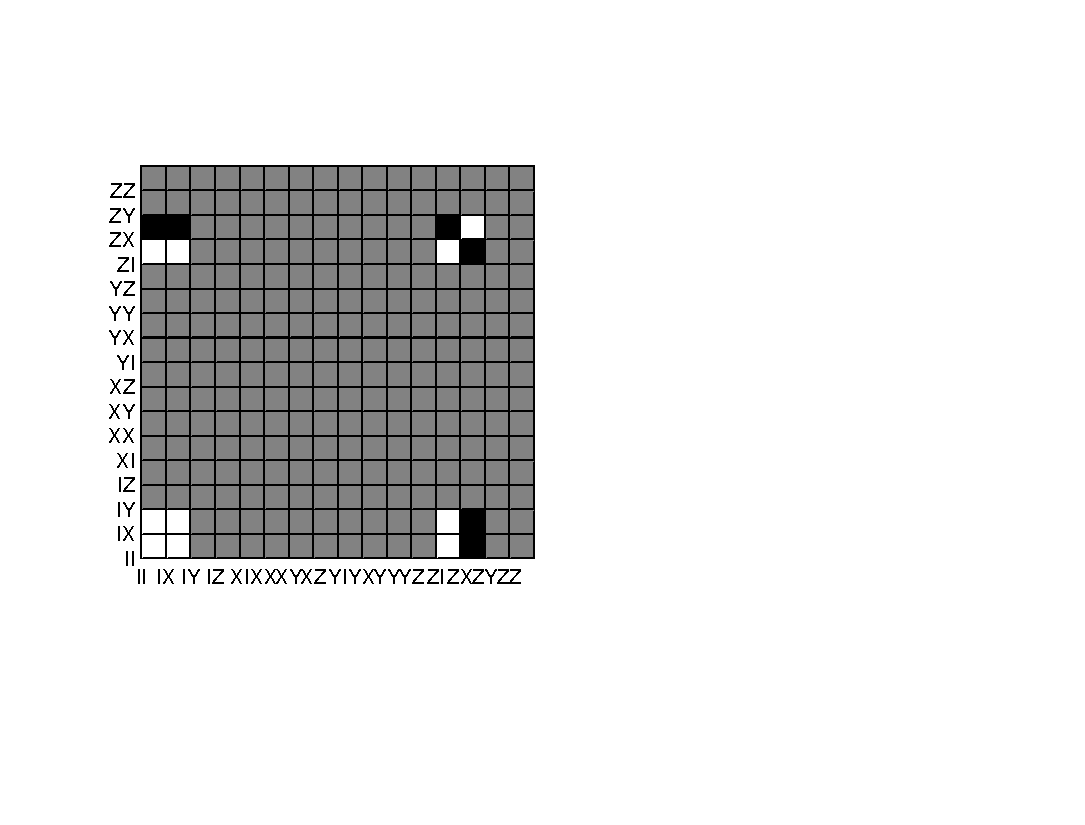
\includegraphics[width=0.7\columnwidth]{CNOT_process}
\caption{Process matrix for the CNOT gate, expressed in the Pauli basis. Colour coding: grey=0, white=$1/4$, black=$-1/4$.} \label{fig:CNOT_proc_matrix}
\end{figure}

%
% Quantum Processes in Quantum Networks
%

\subsection{Quantum processes in quantum networks} \label{sec:quant_proc_in} \index{Quantum processes}

Letting $v_i$ represent the $i$th node within a route $R$, the process associated with communication from that node to the next is $\mathcal{E}_{v_i\to v_{i+1}}$. For the same network used previously, Fig.~\ref{fig:example_proc_graph} shows the quantum processes associated with the links in the network. The cumulative process associated with an entire route is therefore,
\begin{align}
\mathcal{E}_R = \mathcal{E}_{{v_{|R|-1}}\to v_{|R|}} \circ \dots \circ \mathcal{E}_{v_2\to v_3} \circ \mathcal{E}_{v_1\to v_2},
\end{align}
where $|R|$ is the number of nodes in $R$, and to simplify notation, all $v_i$ are implicitly over the route $R$.

\begin{figure}[!htb]
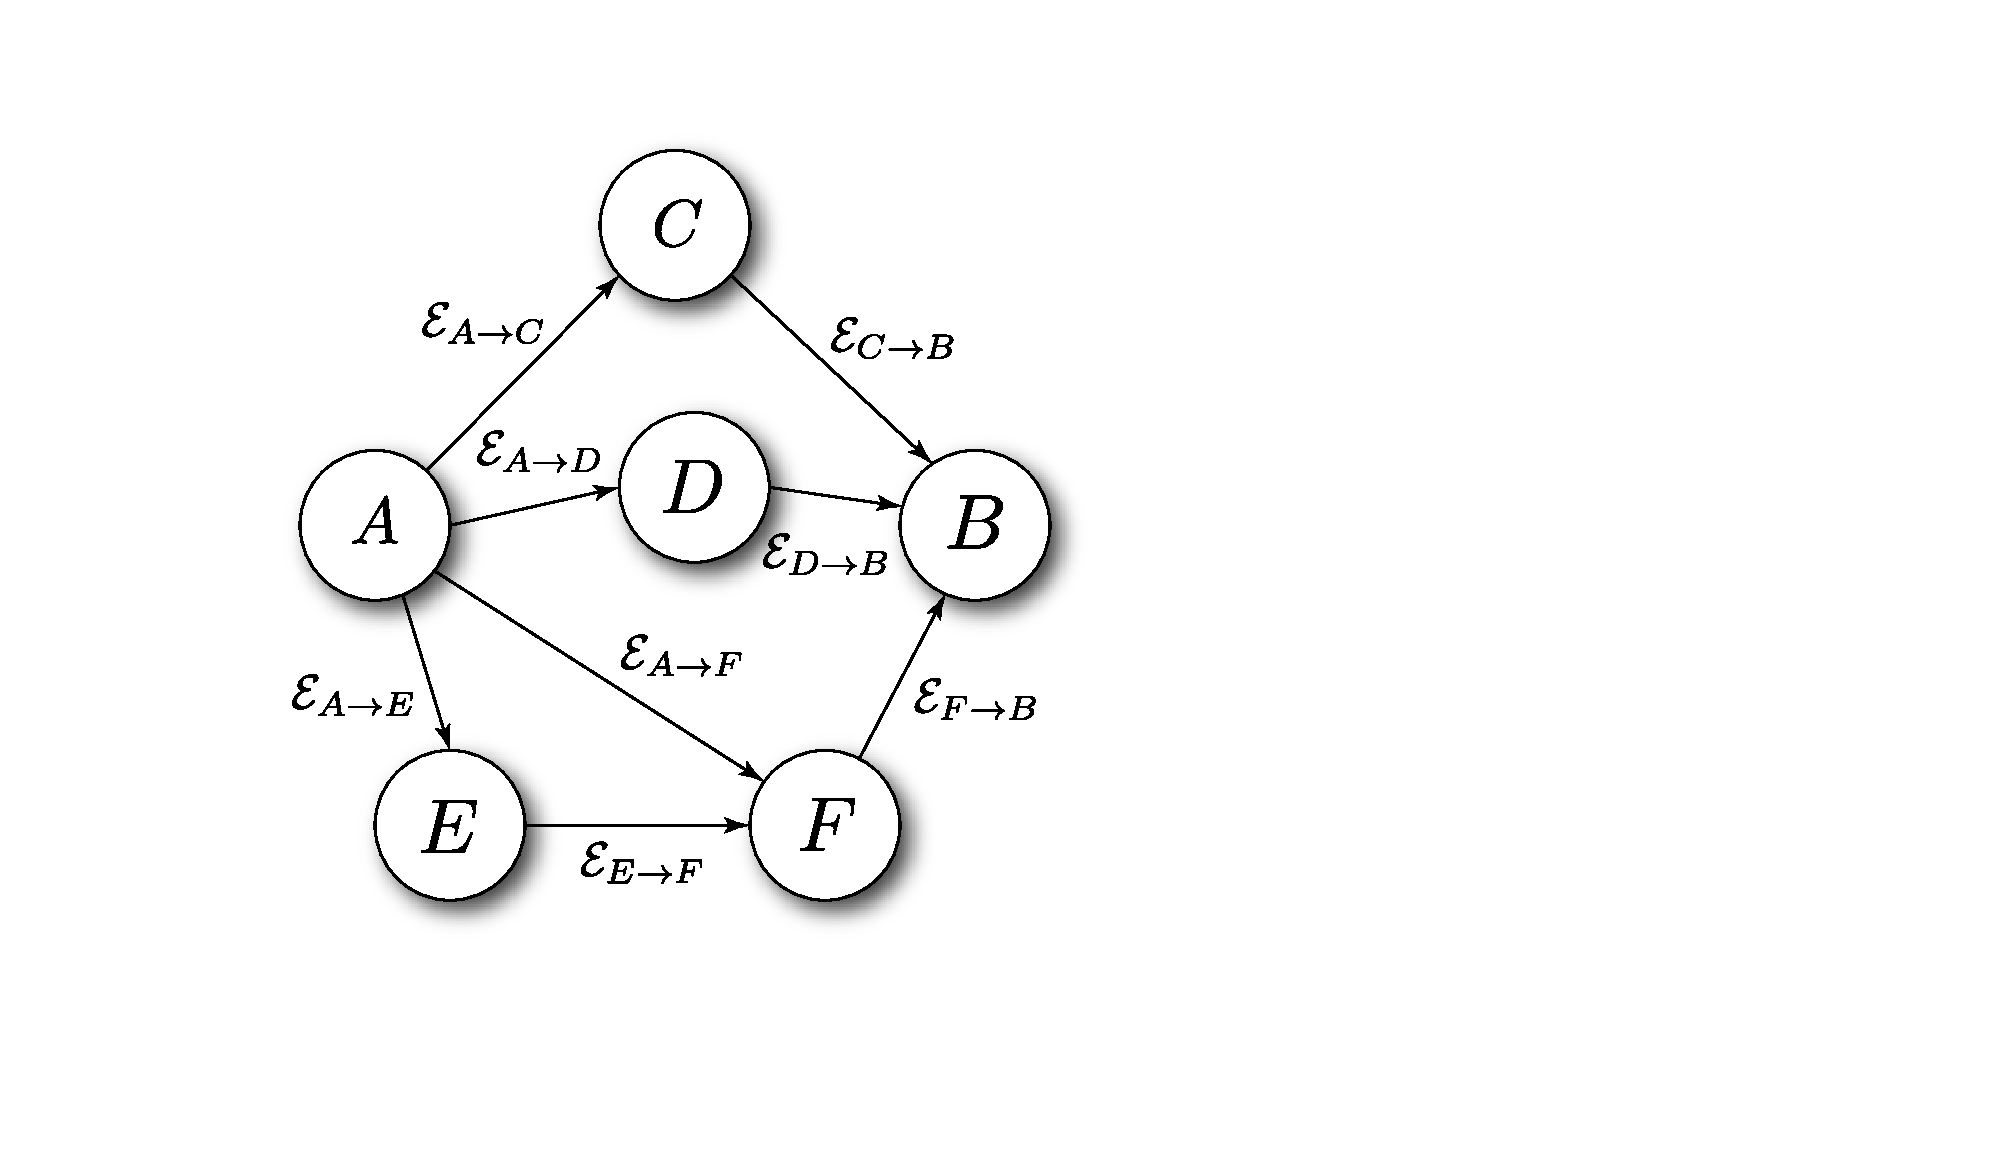
\includegraphics[width=0.6\columnwidth]{example_graph}
\caption{The network from Fig.~\ref{fig:example_routes}, with the quantum processes associated with each link. The net process associated with a route is given by the composition of each of the processes over the length of the route. For example, the route \mbox{$R_1=A\to C\to B$} induces the process \mbox{$\mathcal{E}_{R_1} = \mathcal{E}_{C\to B} \circ \mathcal{E}_{A\to C}$}.} \label{fig:example_proc_graph}
\end{figure}

In general, both nodes and links in a quantum network may implement quantum processes. However, for the purposes of compatibility with the graph-theoretic algorithms described in Sec.~\ref{sec:graph_theory}, we will eliminate node processes by merging them into link processes, such that the processes in the network are described entirely by links. This reduction procedure is straightforward, shown in Fig.~\ref{fig:remove_nodes}.

\begin{figure}[!htb]
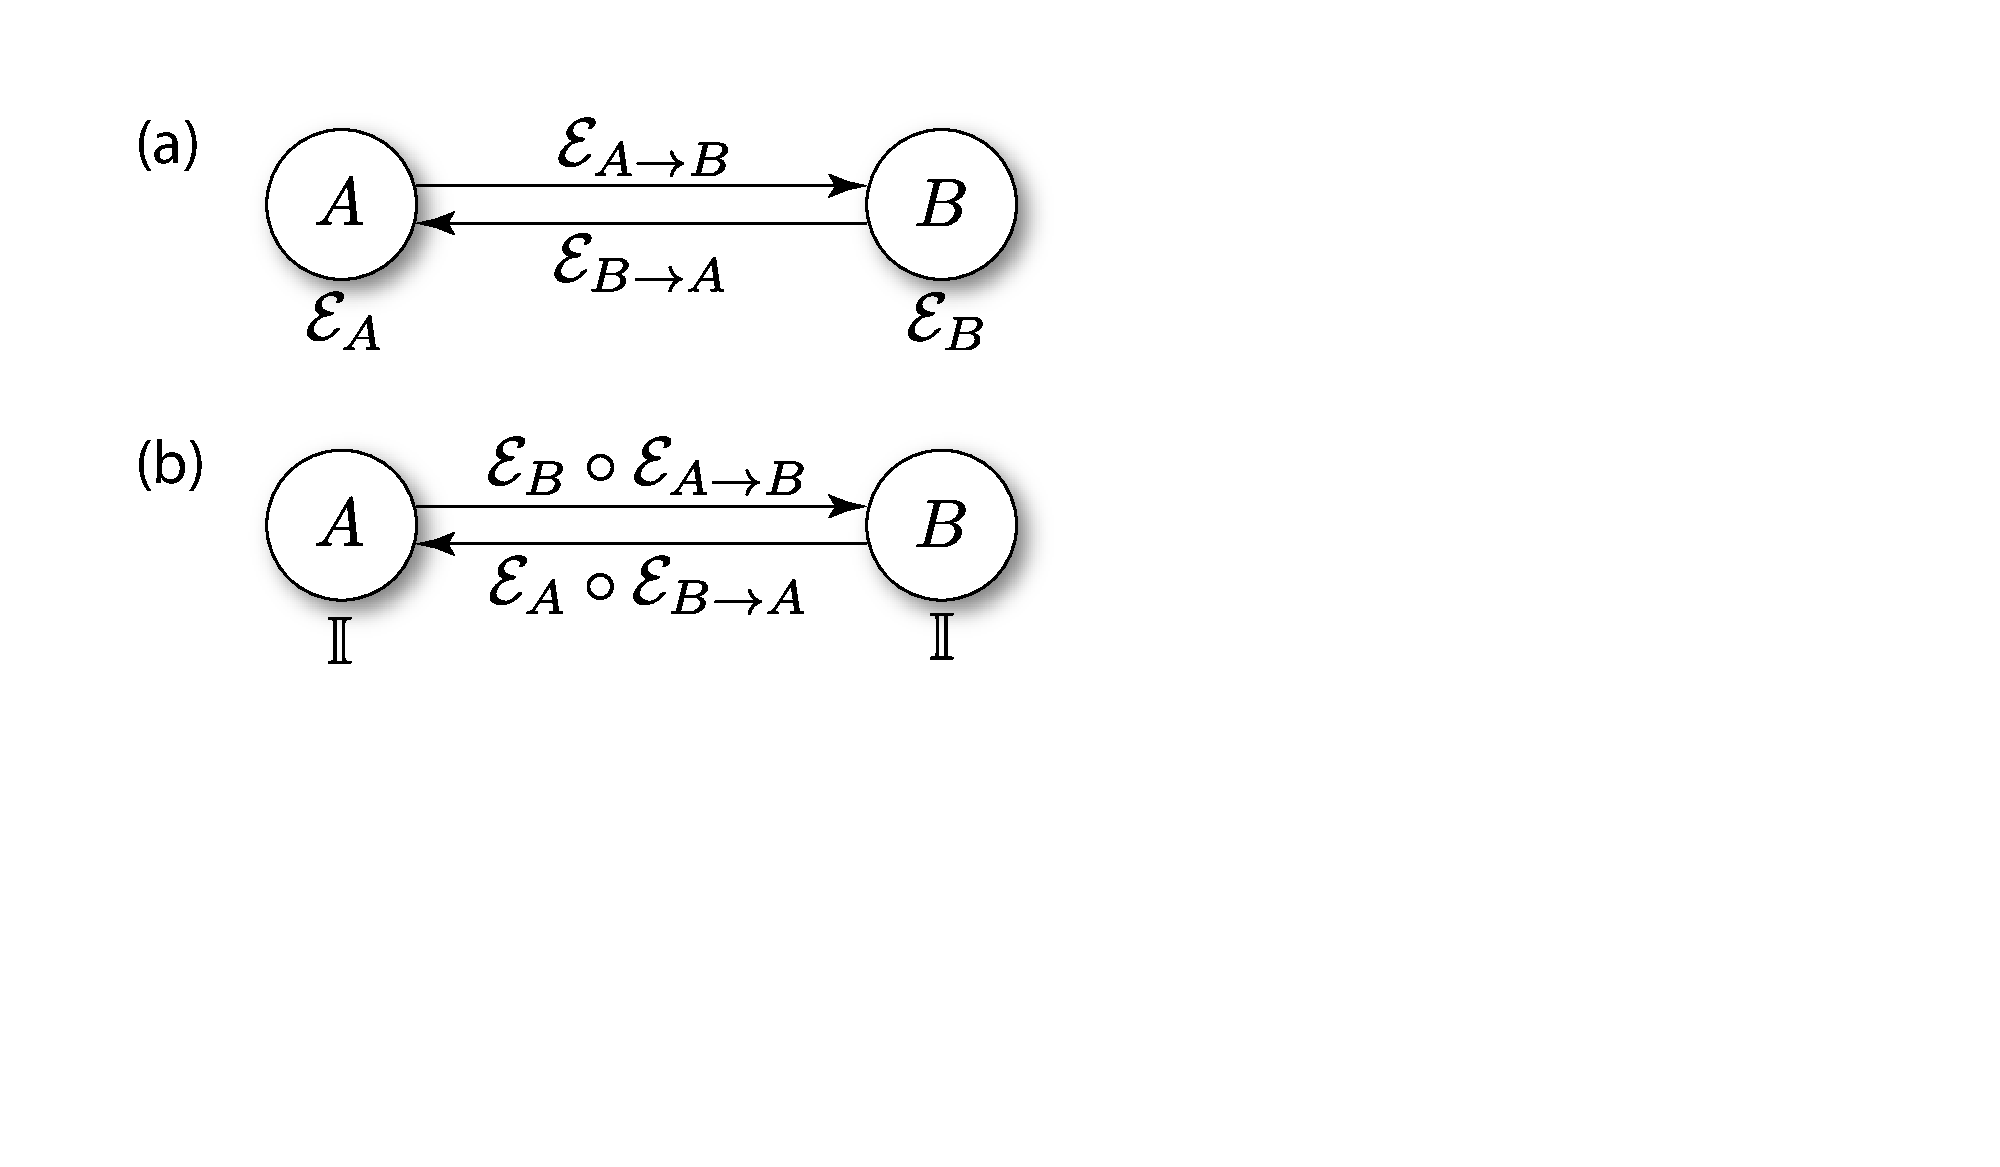
\includegraphics[width=0.7\columnwidth]{remove_nodes}
\caption{Removing node processes from network graphs on a trivial network with two nodes, $A$ and $B$. Each node is associated with a quantum process ($\mathcal{E}_A$ and $\mathcal{E}_B$). Similarly, each link is associated with a process ($\mathcal{E}_{A\to B}$ and $\mathcal{E}_{B\to A}$). (a) Representation where the node and link processes are shown explicitly. (b) The node processes are replaced with identity operations by replacing each link process with the composition of the link process and its target node process. Equivalently, the cost of each node process is added to the cost of \textit{every} incoming link and then eliminated. The same may be applied for attributes rather than costs. This procedure requires that all links be directed. If undirected links are present, they may simply be replaced by two directed links, one in each direction, implementing identical quantum processes each way.} \label{fig:remove_nodes}
\end{figure}

%
% Characterising Quantum Channels
%

\subsection{Characterising quantum states and channels} \label{sec:QPT}

Given a link implementing some arbitrary quantum process, it is essential that it can be experimentally determined such that network performance may be characterised. For example, if an optical channel is lossy, what is the loss rate? This is crucial when attempting to choose routing strategies that optimise certain cost metrics.

Treating a link or node as an unknown black box, \textit{quantum process tomography} (QPT) \cite{bib:ChuangNielsen97, ???} is a technique that may be applied to fully characterise the quantum process it implements, reproducing its complete process matrix. QPT has become a standard procedure, demonstrated in numerous architectures, most notably in optics \cite{bib:OBrien04, bib:RohdeGateChar05}.

QPT works in general for processes in any degree of freedom, e.g the qubit degree of freedom. However, it is important to note that full QPT requires statistics across the entire basis over which measurements are defined, which typically grows exponentially with the size of the system. For example, the number of measurement bases required to perform full QPT on $n$ qubits grows exponentially with $n$.

However, often full process characterisation is not necessary. Instead, knowing particular metrics of interest may suffice. Some of the more noteworthy such metrics will be discussed in Sec.~\ref{sec:quantum_meas_cost}. In this instance, much work has been done in the field of \textit{compressed sensing} or \textit{compressed quantum process tomography} \cite{???,compressed_sensing}, in which some process metrics of interest can be experimentally determined using far fewer physical resources (with efficient scaling!) than via a full reconstruction of the process matrix using QPT. As a most trivial example, if the loss associated with a fibre-optic channel is the metric of interest, this can be much more easily determined than by performing full QPT.

On the other hand, however, most quantum channels are designed to accommodate systems with very limited Hilbert space dimensionality per clock-cycle -- e.g a fibre-optic link might transmit just one photon at a time -- in which case there is no exponentiality to be terribly concerned about (QPT of a single-photon channel is trivial).

Importantly, it is often the case that the quantum process associated with a channel will remain constant over time. The efficiency of a length of fibre, for example, does not change. In this instance, characterising the channel need only be performed once in advance, without requiring ongoing dynamic updating. On the other hand, when communicating with satellites in low Earth orbit it is to be expected that the properties of links will be highly dynamic.

We will now explain QPT in the archetypal context of single-qubit channels, which logically generalises to multiple qubits, and can similarly be generalised to non-qubit systems also.

%
% Quantum State Tomography
%

\subsubsection{Quantum state tomography} \index{Quantum state tomography (QST)}

The first stage in QPT is \textit{quantum state tomography} (QST), where the goal is to reconstruct and unknown density matrix via measurements upon multiple copies of the state. QST is based upon the simple observation that the completeness relation\index{Completeness relation} for an arbitrary state can be expressed,
\begin{align}
\hat\rho = \sum_i \text{tr}(\hat{E}_i\hat\rho)\cdot\hat{E}_i,
\end{align}
where $\{\hat{E}_i\}$ forms a complete basis for the Hilbert space of $\hat\rho$. For a single-qubit this decomposition is most often performed in the Pauli basis, 
\begin{align}
\hat\rho = \text{tr}(\hat\rho)\cdot\hat{\mathbb{I}} + \text{tr}(\hat{X}\hat\rho)\cdot\hat{X} + \text{tr}(\hat{Y}\hat\rho)\cdot\hat{Y} +\text{tr}(\hat{Z}\hat\rho)\cdot\hat{Z}.
\end{align}
Of course, \mbox{$\text{tr}(\hat{E}\hat\rho) = P(\hat{E}|\hat\rho)$} is just the expectation value of the measurement operator $\hat{E}$ when measuring $\hat\rho$. Thus, measuring the expectation values in each of the four Pauli bases reconstructs $\hat\rho$.

This generalises straightforwardly to multi-qubit systems, where we measure all combinations of tensor products of the Pauli operators, the number of which grows exponentially with the number of qubits $n$, as $4^n$. This introduces scalability issues for systems comprising a large number of qubits.

In the case of optical systems, entirely alternate, but equivalent, approaches may be used, such a probing the Wigner function directly using homodyne detection \cite{???}.

%
% Quantum Process Tomography
%

\subsubsection{Quantum process tomography} \index{Quantum process tomography (QPT)}

Now to perform QPT we apply the unknown process to a complete basis of input states $\{\hat\rho_i\}$, and perform QST on the output state for each. This yields,
\begin{align}
\mathcal{E}(\hat\rho_j) = \sum_{i} c_{i,j} \hat\rho_i,
\end{align}
where the sum runs over the basis of states. From QST, all the coefficients $c_{i,j}$ may be determined. Next we define the following decomposition for each of the terms in the sum of Eq.~(\ref{eq:process_matrix}),
\begin{align}
\hat{E}_m \hat\rho_j \hat{E}_n^\dag = \sum_k B^{m,n}_{j,k} \hat\rho_k,
\end{align}
where $B$ defines a decomposition in the chosen basis, not dependent on any measurement results. Then we can write,
\begin{align}
\mathcal{E}(\hat\rho_j) &= \sum_{m,n} \chi_{m,n} \hat{E}_m\hat\rho_j\hat{E}_n^\dag \nonumber \\
&= \sum_{m,n} \sum_k \chi_{m,n} B^{m,n}_{j,k} \hat\rho_k.
\end{align}
Because $\hat\rho_k$ form a linearly independent basis, we can write the decomposition,
\begin{align}
c_{j,k} = \sum_{m,n} \chi_{m,n} B_{j,k}^{m,n},
\end{align}
for all \mbox{$j,k$}. From this, standard linear algebra techniques allow an inversion to obtain,
\begin{align}
\chi_{m,n} = \sum_{j,k} (B_{j,k}^{m,n})^{-1} c_{j,k},
\end{align}
thereby obtaining the full process matrix $\chi$, in the chosen basis.

%
% Optical Encoding of Quantum Information
%

\section{Optical encoding of quantum information} \label{sec:opt_enc_of_qi} \index{Optical encoding of quantum information}

While all-optical quantum computing is an unlikely architecture for future scalable quantum computers, it is all but inevitable that optics will play a central role in quantum communications networks. Foremost, this is because photons are `flying' by their very nature and can very easily be transmitted across large distances -- it's quite challenging to transmit a superconducting circuit containing information from Australia to Mozambique in the blink of an eye! Additionally, optical states are, in many cases, relatively easy to prepare, manipulate and measure, and can also be readily interfaced with other physical quantum systems (Sec.~\ref{sec:opt_inter}), allowing the transfer of quantum information from optical communications systems to some other architecture better suited to a given task.

Optical systems are very versatile, allowing quantum information to be optically encoded in a number of ways -- into single photons, many photons, or even an indeterminate number of photons, and in both discrete or continuous degrees of freedom. Different types of encodings may have very different properties in terms of the errors they are susceptible to (Sec.~\ref{sec:errors_in_nets}).

When dealing with single photons, information can be encoded in a number of ways. Most obviously, it can be encoded into the polarisation basis, allowing one qubit of information per photon (i.e horizontal and vertical polarisation represent the logical $\ket{0}$ and $\ket{1}$ states). Or it could be directly encoded into the photon-number basis. However, other degrees of freedom, such as the spectral/temporal degrees of freedom could be employed, encoding information into time- or frequency-bins, with potentially far more levels than a simple polarisation qubit \cite{bib:RohdeInfCap13}. Next we discuss the main methods for optical encoding of quantum information.

%
% Single Photons
%

\subsection{Single photons} \label{sec:single_phot_enc} \index{Single-photon encoding}

A very attractive feature of single photons is that they undergo very little decoherence, even over large distances -- dephasing (Sec.~\ref{sec:dephasing_error}) in the polarisation degree of freedom, for example, is negligible in free-space. They are, however, very susceptible to loss, and protocols relying on many single-photon states suffer exponential decay in their success rates as the number of photons is increased (Sec.~\ref{sec:eff_err}).

We can encode a single qubit into a single photon in the polarisation basis using the horizontal and vertical polarisation degrees of freedom. Equivalently, one can employ `dual rail' encoding, whereby a single photon is placed into a superposition across two spatial modes. This leads to the equivalent representations for logical qubits ($L$),
\begin{align} \label{eq:single_photon_enc}\index{Polarisation encoding} \index{Dual-rail encoding}
\ket{\psi}_\text{qubit} &\equiv \alpha\ket{0}_L + \beta\ket{1}_L, \nonumber \\
\ket{\psi}_\text{pol} &\equiv \alpha\ket{H} + \beta\ket{V}, \nonumber \\
\ket{\psi}_\text{dual} &\equiv \alpha\ket{0,1} + \beta\ket{1,0}.
\end{align}
Conversion between polarisation and dual-rail encoding is straightforward and deterministic using standard optical components, as described in Fig.~\ref{fig:pol_to_dual_conv}.

\begin{figure}
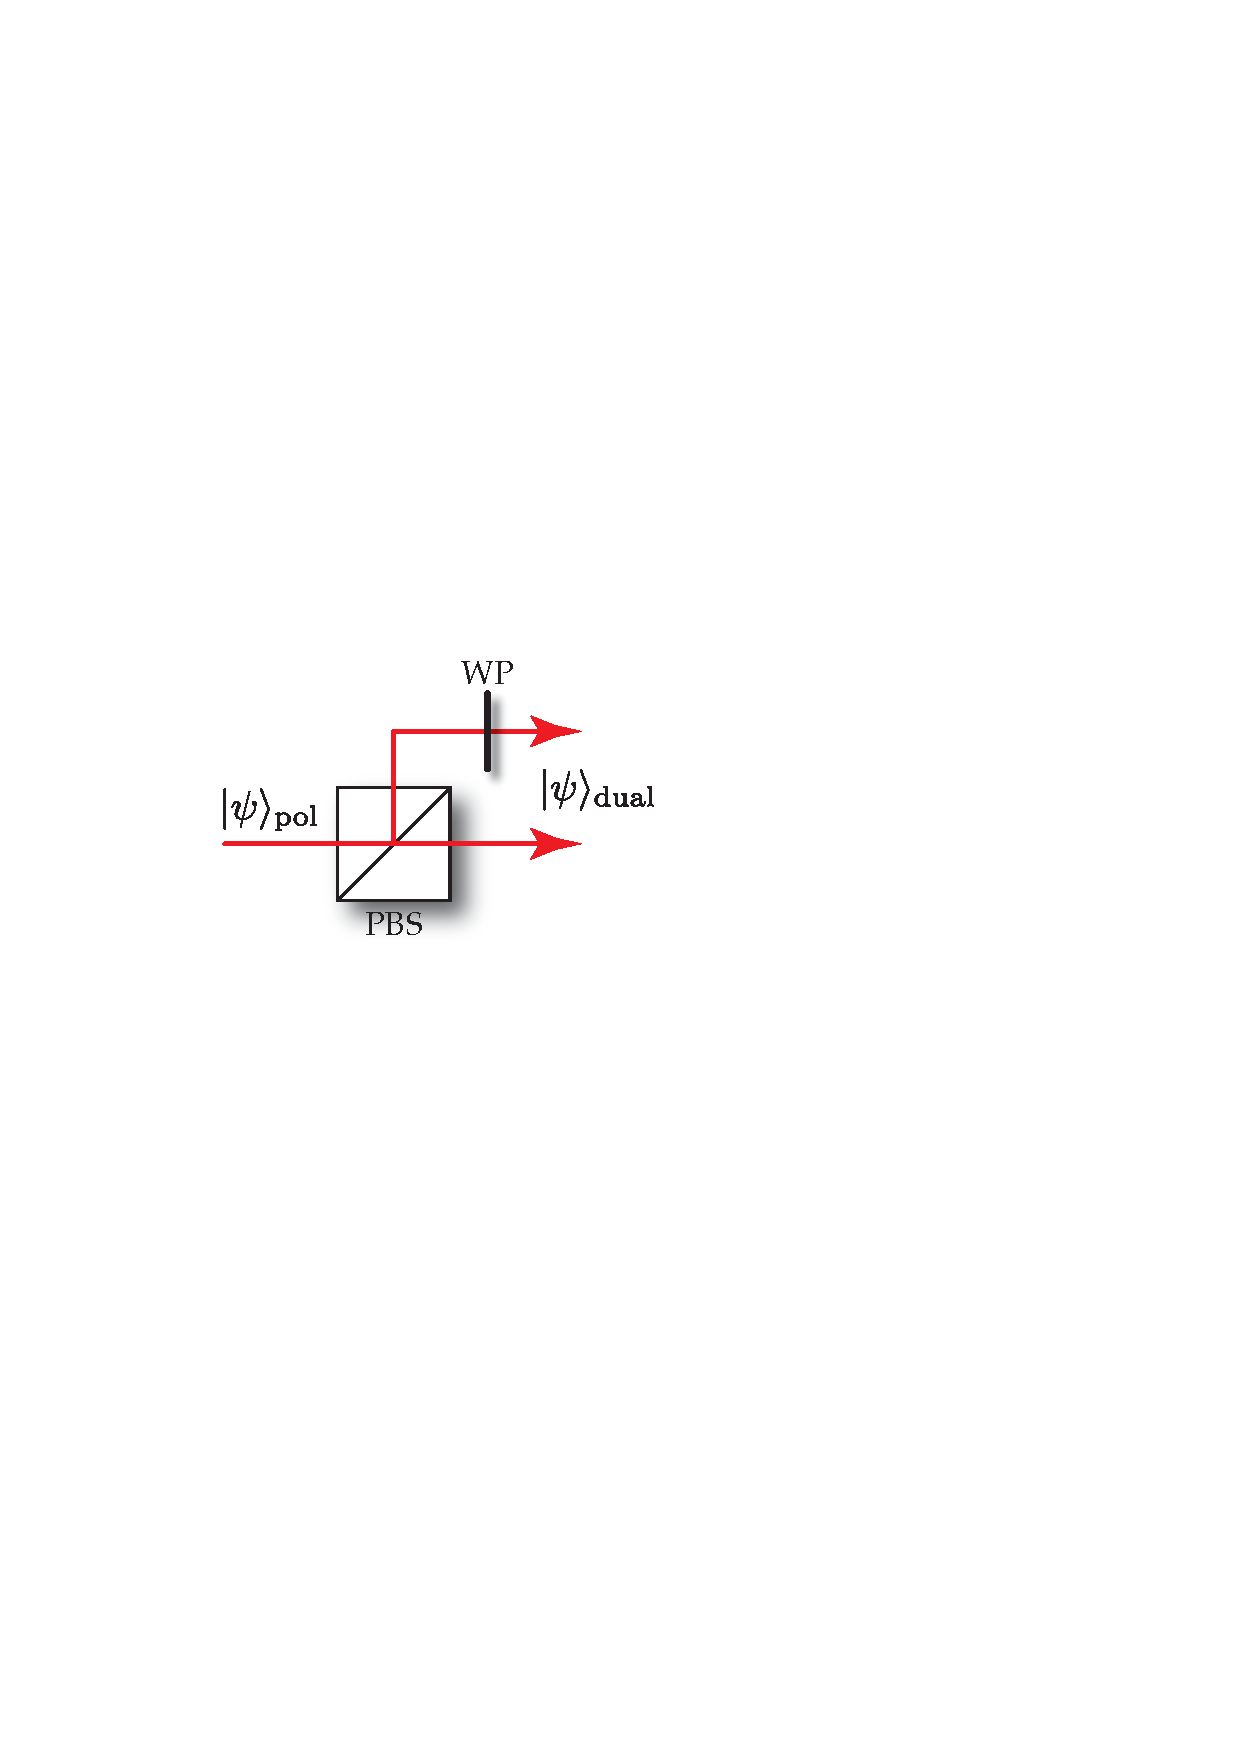
\includegraphics[width=0.6\columnwidth]{pol_to_dual_conversion}
\caption{Conversion from single-photon polarisation encoding to dual-rail encoding, using a polarising beamsplitter (PBS) and wave-plate (WP). The PBS separates the polarisation components into two distinct spatial modes. The WP then rotates the polarisation of one of the spatial modes such that it has the same polarisation as the other. Conversion from dual-rail to polarisation encoding is just the reverse of this procedure.} \label{fig:pol_to_dual_conv}\index{Polarising beamsplitters}
\end{figure}

Note that polarisation encoding requires a single spatial mode per qubit, whereas dual-rail encoding requires two. Polarisation encoding brings with it the advantage that arbitrary single-qubit operations may be implemented using wave-plates, which maintain coherence between the basis states extraordinarily well. In dual-rail encoding, on the other hand, single-qubit operations are implemented using beamsplitter operations between the two spatial modes, which must be interferometrically stable, since consecutive single-qubit operations yields Mach-Zehnder (MZ) interference \cite{bib:Zehnder1, bib:Zehnder2}\index{Mach-Zehnder (MZ) interference}, to be discussed in detail in Sec.~\ref{sec:MZ_inter}.

Single-photon encodings are extremely important, as they form the basis for universal linear optics quantum computing (Sec.~\ref{sec:KLM_univ}), \textsc{BosonSampling} (Sec.~\ref{sec:BS}) and quantum walks (Sec.~\ref{sec:QW}). They are also the simplest optical states for representing single qubits.

%
% Photon-number
%

\subsection{Photon-number} \index{Photon-number encoding}

Of course, the photon-number degree of freedom needn't be limited to 0 or 1 photons. By fully exploiting the photon-number degree of freedom, we can encode a qudit of arbitrary dimension into a single optical mode,
\begin{align} \label{eq:number_qudit}
\ket\psi_\text{qudit} \equiv \sum_{n=0}^\infty \alpha_n \ket{n}.
\end{align}
This may give the impression that a single optical mode has infinite information capacity. Needless to say, this sounds too good to be true, and it is. Loss decoheres photon-number-encoded states exponentially with photon-number, since for large photon-number the probability of a number state retaining its photon-number exponentially asymptotes to zero. So although in principle we can encode an $\infty$-level qudit, the moment any non-zero loss is introduced, this exponential dependence destroys the state (Sec.~\ref{sec:eff_err}).

While photon-number encoding can be useful for communications purposes, it is not very practical for quantum information processing tasks, since operations between basis states are not energy preserving, with each basis state having energy \mbox{$E=n\hbar\omega$}, where $\omega$ is frequency, and $\hbar$ is Planck's constant. Thus, qudit operations would need to be active processes.

%
% Spatio-Temporal Qudit Encoding
%

\subsection{Spatio-temporal} \label{sec:spatio_temporal} \index{Spatio-temporal encoding}

Completely independent of the photon-number degree of freedom, are the spatio-temporal degrees of freedom, which encode the spatial, temporal, and spectral/temporal structure of photons. In the temporal domain, for example, we could define the temporal structure of a single photon as,
\begin{align}
\ket\psi_\text{temporal} = \int_{-\infty}^\infty \psi(t) \hat{a}^\dag(t)\,dt\,\ket{0},
\end{align}
where $\hat{a}^\dag(t)$ is the time-specific photonic creation operator, and $\psi(t)$ is the temporal distribution function \cite{bib:RohdeFreqTemp05}.

Alternately, we can define \textit{mode operators} \cite{bib:RohdeMauererSilberhorn07}\index{Mode operators}, which are mathematically equivalent to creation operators, but create photons with a specific temporal envelope,
\begin{align}
\hat{A}^\dag_\psi &= \int_{-\infty}^\infty \psi(t) \hat{a}^\dag(t)\,dt, \nonumber \\
\ket\psi_\text{temporal} &= \hat{A}^\dag_\psi \ket{0}.
\end{align}
Mode operators commute, inheriting this property directly from photonic creation operators,
\begin{align}
\left[\hat{A}^\dag_{\psi_1},\hat{A}^\dag_{\psi_2}\right]=0.
\end{align}

Now by defining an orthonormal basis of temporal distribution functions, $\{\xi_i\}$, such that,
\begin{align} \label{eq:spec_orth_def}
\bra{0} \hat{A}_{\xi_i} \hat{A}^\dag_{\xi_j}\ket{0} = \delta_{i,j},
\end{align}
we can encode a qudit of arbitrary dimension into the spatio-temporal degrees of freedom,
\begin{align}
\ket\psi_\text{qudit} \equiv \sum_{i=0}^\infty \alpha_i \hat{A}^\dag_{\xi_i} \ket{0}.
\end{align}

This encoding allows a qudit of arbitrary dimension to be encoded into a single spatial mode. Again, however, summing to infinity is somewhat fanciful, given any physically realistic spatio-temporal error model, such as an imperfect frequency response in the channel, e.g a bandpass response of an optical fibre or photo-detector.

%
% Time-Bins
%

\subsection{Time-bins} \label{sec:time_bin} \index{Time-bin encoding}

In time-bin encoding we define our basis of modes (whether it be qubits or higher-dimensional qudits) as distinct, non-overlapping time-bins, which are localised wave-packets in the temporal degree of freedom, each separated from the next by some fixed interval $\tau$. This can be considered a special case of spatio-temporal encoding, where the basis mode functions satisfy the relation,
\begin{align}
\xi_{j}(t) = \xi_0(t-j\tau),
\end{align}
as well as the usual orthonormality constraints. Here $\tau$ is sufficiently large, and $\xi_i(t)$ sufficiently temporally localised, that the temporal modes are orthogonal as per Eq.~(\ref{eq:spec_orth_def}).

Time-bin encoding arises naturally in architectures where the photon source driving the system is operating at a high repetition rate\index{Repetition rate}, $R$, in which case \mbox{$\tau=1/R$}. Architectures for optical quantum computing have been described \cite{bib:RohdeLoop15, bib:RohdeUnivLoop15}, and experimentally demonstrated \cite{???}, based entirely on time-bin encoding.

These schemes can be very resource efficient, since a single source operating at high repetition rate can replace an entire bank of distinct sources that would ordinarily be required in spatial architectures. Similarly, a single time-resolved detector, with resolution at least $\tau$, can replace a bank of detectors operating in parallel. And only a single spatial mode is required to store an arbitrary number of qubits/qudits, so long as it is long enough to support the entire pulse-train -- at least $2n\tau$ for $n$ qubits.

In the schemes of \cite{bib:RohdeLoop15, bib:RohdeUnivLoop15}, entire optical quantum computing protocols can be efficiently constructed using only a single source, a single detector, two delay-lines, and three dynamically-controlled beamsplitters, irrespective of the size of the computation, an enormous resource saving compared to traditional spatial encodings. Furthermore, in these schemes, there is only a single point of interference, greatly simplifying optical interferometric alignment, which would ordinarily require simultaneously aligning a large number of optical elements, as many as $O(m^2)$ elements for an $m$-mode network \cite{bib:Reck94}.

%
% Coherent States
%

\subsection{Coherent states} \label{sec:coherent_state_enc} \index{Coherent state encoding}

When encoding information optically, we needn't restrict ourselves to photon-number states. We also have a lot of flexibility to encode information in phase-space using continuous variable (CV) states, where phase and amplitude relations encode quantum information \cite{bib:CahillGlauber69}.

As a simple example, consider coherent states. These are particularly useful since they are pure states, with well defined coherence relationships, and are closely approximated by laser sources, and therefore readily available in the lab.

A coherent state, $\ket\alpha$, is parameterised by a single complex parameter, $\alpha$, given by a phase and amplitude,
\begin{align}\index{Coherent states}
\ket{\alpha} = e^{-\frac{|\alpha|^2}{2}} \sum_{n=0}^\infty \frac{\alpha^n}{\sqrt{n!}} \ket{n}.
\end{align}
By manipulating these parameters, information can be encoded into coherent states. We could, for example, define two coherent states of opposite phase to represent qubit basis states,
\begin{align}
\ket{0} &\equiv \ket{\alpha}, \nonumber \\
\ket{1} &\equiv \ket{-\alpha}.
\end{align}
Note, however, that this representation for qubits is only approximate, since the two basis states are not perfectly orthogonal,
\begin{align}
\langle -\alpha|\alpha \rangle = e^{-2|\alpha|^2},
\end{align}
which is non-zero for any finite $\alpha$, whereas for ideal qubits we require \mbox{$\langle 0|1\rangle = 0$}. However, for large $\alpha$, $\ket{\pm\alpha}$ closely approximate orthogonality.

This representation for qubits using coherent states is easily generalised to qudits by considering coherent states orbiting the origin of phase-space at equal angular intervals of \mbox{$2\pi/d$}, for a $d$-level qudit. The $k$th qudit basis state is then,
\begin{align}
\ket{k}_d = \ket{e^{ik/d}\alpha},
\end{align}
for \mbox{$k=0,\dots,d-1$}, where again the basis states are non-orthogonal, but closely approximate orthogonality for large $\alpha$.

Note that despite being pure states, with well-defined coherence, coherent states are considered classical, as they are unable to encode quantum information. That is, the coherence relationships cannot be exploited for the encoding of qubits or qudits.

Coherent states are useful in that they are easy to prepare using modern lasers, including laser diodes, and by turning up the amplitude can be transmitted over long distances, with loss not affecting quantum coherence, only the amplitude (Sec.~\ref{sec:eff_err}).

%
% Cat States
%

\subsection{Cat states} \label{sec:cat_enc} \index{Cat state encoding}\index{Cat states}

Another type of CV state, which can in fact encode quantum information, is superpositions of coherent states (colloquially known as `cat' states), with the encoding \cite{???},
\begin{align}
\ket{0} &\equiv \frac{1}{\sqrt{2(1+e^{-2|\alpha|^2})}} (\ket{\alpha}+\ket{-\alpha}) \nonumber \\
&= \ket{\text{cat}_+(\alpha)},\nonumber \\
\ket{1} &\equiv \frac{1}{\sqrt{2(1-e^{-2|\alpha|^2})}}(\ket{\alpha}-\ket{-\alpha}) \nonumber \\
&= \ket{\text{cat}_-(\alpha)}.
\end{align}
These two basis states contain strictly even or odd photon-number terms respectively (i.e they have well-defined parity), implying that, unlike coherent states, they are always orthogonal, regardless of amplitude,
\begin{align}
\langle\text{cat}_+(\alpha)|\text{cat}_-(\alpha)\rangle = 0 \,\,\forall\,\alpha,
\end{align}
making them directly appropriate for qubit encoding, even for weak coherent amplitudes.

Unfortunately, cat states are notoriously difficult to prepare, and extremely sensitive to loss (Sec.~\ref{sec:single_phot_enc}) and dephasing (Sec.~\ref{sec:dephasing_error}). This arises because loss of a single photon flips the parity of the state to an orthogonal one, meaning that as $\alpha$ increases, the state is exponentially more susceptible to becoming a mixture of the logical basis states.

However, modulo these difficulties, with a resource of cat states at one's disposal, universal quantum computation may be realised using post-selected linear optics \cite{bib:JeongRalph05, bib:Gilchrist04}.

%
% Thermal State Encoding
%

\subsection{Thermal states} \index{Thermal state encoding}\label{sec:thermal_states}

In some quantum protocols, although the inner workings may be quantum mechanical in nature, the inputs and outputs needn't capture any quantum coherence -- sometimes \textit{classical} information is sufficient for communications. As discussed above, coherent states are the archetypal example of this, and this is in fact the norm in present-day classical fibre-optic communication, where coherent states prepared from laser diodes are employed.

Another, and even simpler option, is thermal states. These are obtained by fully dephasing a coherent state, retaining the amplitudes, while nullifying all the coherence terms,
\begin{align}
\hat\rho_\text{thermal}(\alpha) = e^{-|\alpha|^2} \sum_{n=0}^\infty \frac{|\alpha|^2}{n!}\ket{n}\bra{n}.
\end{align}

Thermal states can encode classical information into their amplitudes, polarisations, or time-bins, as before. The advantage of this type of encoding is that thermal states are trivial to prepare and measure (a normal incandescent lightbulb produces thermal states of light). However, they are purely classical states, do not undergo interference with one another, and are therefore useless for, for example, entangling qubits via which-path erasure, any other type of coherent interferometric process, or for representing quantum information such as qubits.

%
% Phase-Space
%

\subsection{Phase-space} \label{sec:exotic} \index{Phase-space encoding}

The optical encodings presented thus far are the main textbook examples. However, many other encodings, particularly in phase-space, can also be used to encode both quantum or classical information and perform quantum computations upon them. The aforementioned coherent states and cat states are classic examples of states well-suited to a phase-space representation. But this extends to many other states, such as Gaussian states more generally.

In phase-space, the most common representations of optical states are in terms of quasi-probability functions:
\begin{itemize}\index{$P$-function}\index{$Q$-function}\index{Wigner function}
\item $P$-function: represents a state as a quasi-mixture of coherent states. When the $P$-function is strictly non-negative, it can be interpreted as a perfect classical mixture of coherent states. However, with any negativity this classical interpretation breaks down, hence `quasi'-probability. In general, the $P$-function representation for a state is not unique.
\begin{align}
\hat\rho = \int\!\!\!\int P(\alpha) \ket{\alpha}\bra{\alpha} d^2\alpha.
\end{align}
\item $Q$-function: represents a state in terms of its overlap with the complete set of all coherent states, which form an over-complete basis.
\begin{align}
Q(\alpha) = \frac{1}{\pi} \bra{\alpha}\hat\rho\ket{\alpha}.
\end{align}
\item Wigner function: also has a quasi-probability interpretation, and negativity is qualitatively associated with `quantumness'. The Wigner function of a state is unique, and isomorphic to the density operator, making it perhaps the most useful phase-space representation for quantum states of light.
\begin{align}
W(x,p) = \int e^{ips/\hbar} \left\langle{x-\frac{s}{2}}\right| \hat\rho \left|{x+\frac{s}{2}}\right\rangle ds.
\end{align}
\end{itemize}
These representations, whilst entirely equivalent to a photon-number basis representation, are far easier to work with for many types of states. Most notably, Gaussian states are conveniently represented and manipulated using phase-space representations.

%
% Non-Optical Encoding
%

\subsection{Non-optical encoding}\index{Non-optical encodings}

In a non-optical context, the elementary unit of quantum information -- the qubit -- can be naturally encoded into any system with a natural or engineered two-level structure. This actually encompasses a broad range of possibilities, including, amongst many others:
\begin{itemize}
\item \index{2-level systems}Two-level atoms: let two distinct electron energy levels, with long lifetimes, represent the two logical basis states.
\item \index{$\lambda$-configuration systems}$\lambda$-configuration atoms: atoms with two degenerate ground states, which encode the logical qubit, and an additional excited state, which may be transitioned to upon excitation from only one of the ground states. Relaxation from the excited state enables optical coupling via the emitted photon.
\item \index{Quantum dots}Quantum dots: are essentially artificial atoms, which can be engineered with custom band-structures, allowing two- or higher-level qudits to be easily fabricated.
\item \index{Nitrogen-vacancy (NV) centres}Nitrogen-vacancy (NV) centres: are a type of point defect in diamond, which has a very well defined energy level structure that may be utilised to represent qubits.
\item \index{Atomic ensembles}Atomic ensembles: encode quantum information similarly to a single atom, except that the excitation is a \textit{collective} one, in superposition across all the atoms in the ensemble.
\item \index{Superconducting rings}Superconducting rings: a superposition of current flow direction in a superconducting ring represents the two logical basis states.
\item \index{Trapped ions}Trapped ions: qubits are encoded into stable electronic states of electromagnetically trapped ions.
\end{itemize}

Clearly the non-optical elements in a quantum network must somehow interface with optical states, such that communication is facilitated. This is discussed later in Sec.~\ref{sec:opt_inter}.

%
% Errors in Quantum Networks
%

\section{Errors in quantum networks} \label{sec:errors_in_nets} \index{Errors in quantum networks}

As with classical data, quantum data is susceptible to corruption during transmission. However, in addition to all the usual classical error models, quantum information is subject to further uniquely quantum errors. These errors can be represented using the quantum process formalism and fully characterised using QPT (Sec.~\ref{sec:QPT}). We now briefly discuss several of the dominant errors arising in quantum systems, paying especial attention to error models acting on qubits and optical states, as these are the most relevant in a quantum networking context.

%
% Known Unitaries
%

\subsection{Known unitaries} \index{Unitary errors}

The most trivial error mechanism is when a (potentially multi-qubit) unitary channel (e.g an identity channel for the purposes of quantum memory) actually implements some unitary transformation, $\hat{U}$, that is not that which is desired. However, the unitary is constant, not varying from trial to trial, and is known, which can be easily determined by performing QPT on the channel. For example, an optical fibre might induce a polarisation rotation on transmitted photons, but the fibre isn't changing and neither is the rotation. If consistently implementing the same known unitary then reversing it is straightforward in most architectures, by applying $\hat{U}^\dag$, since $\hat{U}^\dag\hat{U}=\hat{\mathbb{I}}$.

%
% Unknown Unitaries
%

\subsection{Unknown imperfect unitaries} \index{Unitary errors}

Alternate to known unitaries, the unitary operation implemented by a node/channel may deviate from that which is desired, in an unknown manner, thereby implementing a slightly different operation than that which we intended to engineer. Specifically, the effective unitary can be represented as the ideal unitary, augmented by some deviation matrix,
\begin{align}
	\hat{U}_\text{effective} = \hat{U}_\text{ideal} + \hat{\Delta}_\text{error},
\end{align}
where the matrix elements of $\hat{\Delta}_\text{error}$ are unknown, but hopefully small. Since the unknown deviation matrix needn't be constant, it will be a function of random variables, evaluated independently for each trial of the process. Furthermore, since the deviation matrix may vary from trial to trial, QPT cannot be employed to characterise it, unlike unitaries with fixed errors.

%
% Loss
%

\subsection{Loss} \label{sec:eff_err} \index{Loss channel}

Given that quantum communication links will typically be optical, the dominant error mechanism is likely to be loss. We let the efficiency, $\eta$, of an optical quantum process be the probability that a given photon entering the channel leaves the channel in the desired mode, or probability \mbox{$1-\eta$} of being lost. In the case of information encoded into single-photon states, e.g using the polarisation degree of freedom, $\eta$ corresponds exactly to the success probability of the communication.

When implementing protocols employing post-selection upon detecting all photons, the protocol will be non-deterministic, where loss dictates the protocol's success probability. Specifically, with $n$ photons, each with efficiency $\eta$, the net post-selection success probability of the entire device is $\eta^n$. This implies an exponential number of trials, \mbox{$(1/\eta)^n$}, is required in post-selected protocols. Clearly this exponential scaling is of concern, requiring demanding efficiencies in future large-scale implementations.

Formally, let $\mathcal{E}^\text{loss}_\eta$ be the loss channel with efficiency $\eta$. The channel acting on an initially pure single-photon state, $\ket{1}$, can be modelled as a beamsplitter with transmissivity $\eta$ acting on the state, where the reflected mode is traced out, shown in Fig.\ref{fig:loss_model}. This yields the quantum process,
\begin{align}
\mathcal{E}^\text{loss}_\eta(\hat\rho) = \text{tr}_B[\hat{U}_\text{BS}(\hat\rho_A\otimes\ket{0}_B\bra{0}_B)\hat{U}_\text{BS}^\dag],
\end{align}
where $\hat{U}_\text{BS}$ is the beamsplitter operation. In the special case of the vacuum and single-photon states, which is most relevant to qubit encodings, we obtain,
\begin{align}
	\mathcal{E}^\text{loss}_\eta(\ket{0}\bra{0}) &= \ket{0}\bra{0}, \nonumber \\
\mathcal{E}^\text{loss}_\eta(\ket{1}\bra{1}) &= (1-\eta)\ket{0}\bra{0} + \eta\ket{1}\bra{1}.
\end{align}
This dynamic is of the same form as amplitude damping (Sec.~\ref{sec:amp_damp}). In the general case of an $n$-photon Fock state, we obtain,
\begin{align}
	\mathcal{E}^\text{loss}_\eta(\ket{n}\bra{n}) = \sum_{i=0}^n \binom{n}{i} \eta^i(1-\eta)^{n-i} \ket{i}\bra{i}.
\end{align}

\begin{figure}[!htb]
	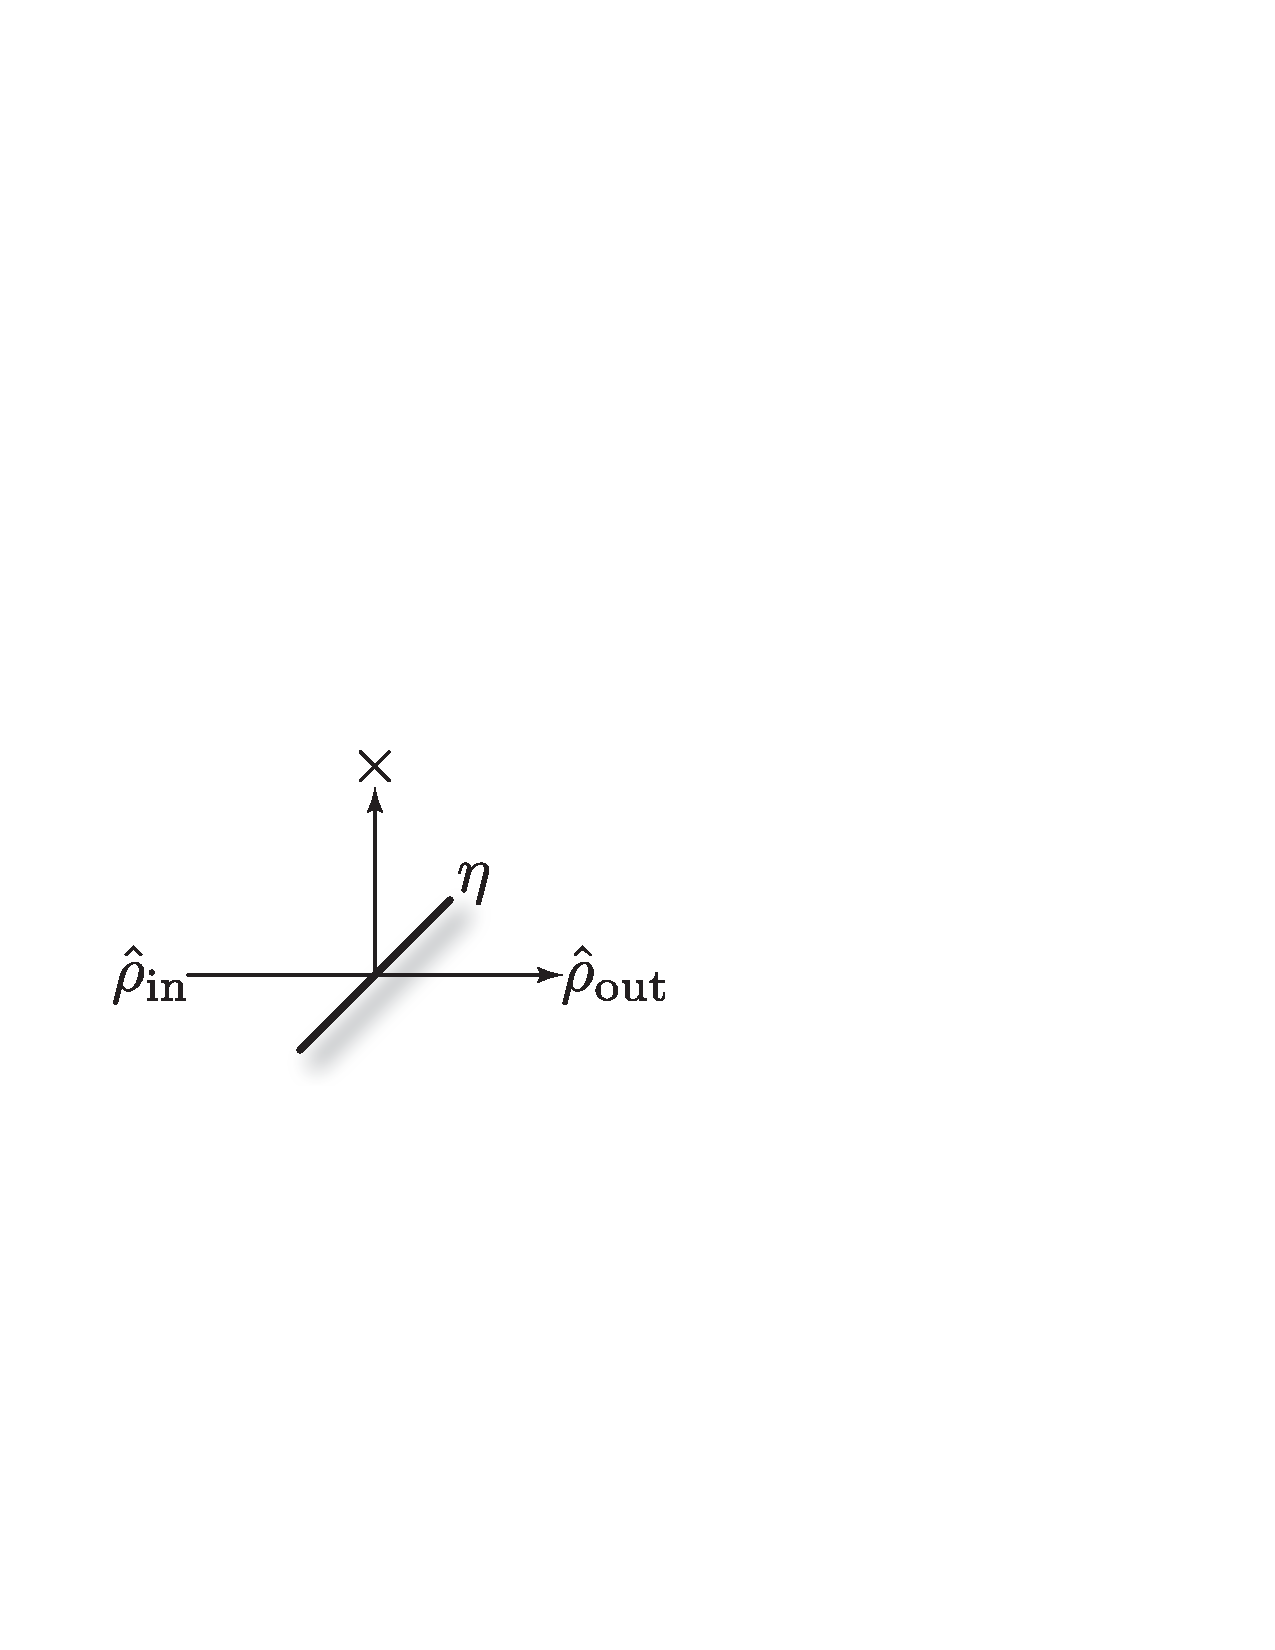
\includegraphics[width=0.5\columnwidth]{loss_model}
	\caption{Model for the loss channel. The input state, $\hat\rho_\text{in}$, passes through a beamsplitter of transmissivity $\eta$, and the reflected mode discarded, yielding the lossy output state \mbox{$\hat\rho_\text{out} = \mathcal{E}^\text{loss}_\eta(\hat\rho_\text{in})$}.} \label{fig:loss_model} \index{Loss channel}
\end{figure}

Consecutive loss channels act multiplicatively,
\begin{align}
\mathcal{E}_{\eta_1}^\text{loss} \circ \mathcal{E}_{\eta_2}^\text{loss} = \mathcal{E}_{\eta_1 \eta_2}^\text{loss}.
\end{align}
In the special case of linear optics circuits, loss channels have the elegant property that, provided the loss rate is uniform across all modes, they can be commuted through the circuit to the front or back \cite{???}\index{Loss commutation}. Specifically,
\begin{align}
(\mathcal{E}_{\eta}^\text{loss})^{\otimes m} \circ \mathcal{E}_U = \mathcal{E}_U \circ (\mathcal{E}_{\eta}^\text{loss})^{\otimes m},
\end{align}
where $\mathcal{E}_U$ is a unitary linear optics process, implementing a photon-number-preserving map of the form of Eq.~(\ref{eq:LO_unitary_map}). This simplifies the treatment of distinct system inefficiencies (such as source, network and detector inefficiencies) by allowing us to commute them to the beginning or end of the circuit and combine them together into a single net efficiency. In many scenarios, this allows the different system inefficiencies to be dealt with via post-selection.

This process would apply equivalently to both horizontal and vertical polarisations. Therefore, via linearity, the loss channel acting on a polarisation-encoded qubit (Sec.~\ref{sec:single_phot_enc}) yields,
\begin{align}
\mathcal{E}^\text{loss}_\eta(\ket\psi_\text{pol}\bra\psi_\text{pol}) = (1-\eta) \ket{0}\bra{0} + \eta\ket\psi_\text{pol}\bra\psi_\text{pol}.
\end{align}
The same applies in the context of dual-rail encoding. Note that while this transformation mixes the state in the photon-number degree of freedom, it preserves coherence between the horizontal and vertical single-photon components. Thus, upon successful post-selection, the state is projected back onto the desired qubit state.

In the case of higher order photon-number encoding of qudits, as per Eq.~(\ref{eq:number_qudit}), the probability of an $n$-photon basis state being maintained scales as $\eta^n$. That is, if the highest photon-number term in our qudit is $n$, that component has an exponentially low probability of being preserved through the loss channel. For this fundamental reason, photon-number encoding does not enable infinite-dimensional qudits to be encoded.

Coherent states are the one example of states, which are in a sense robust against loss, since a lossy coherent state is another coherent state with lower amplitude, but without any loss in coherence,
\begin{align}
\mathcal{E}^\text{loss}_\eta(\ket\alpha\bra\alpha) = \ket{\eta\alpha}\bra{\eta\alpha}.
\end{align}
This arises because coherent states are eigenstates of the photonic annihilation operator, \mbox{$\hat{a}\ket{\alpha}=\alpha\ket{\alpha}$}.

However, although coherence is maintained under the loss channel, the process is irreversible, since noise-free amplitude amplification is not possible in general \cite{???}. Thermal states exhibit the same property, that a loss channel simply yields another thermal state with reduced amplitude, although these exhibit no coherence.

To the contrary, while cat states (Sec.~\ref{sec:cat_enc}) are simple superpositions of coherent states, they are extremely sensitive to loss. This is because cat states have well-defined photon-number parity (strictly even or odd photon-number), and therefore the loss of just a single photon will flip a cat state to an orthogonal one. Since the probability of photon loss occurring increases exponentially with photon-number, large amplitude cat states are exponentially sensitive to loss channels.

Similarly, NOON states (Sec.~\ref{sec:NOON}) undergo complete wavefunction collapse if just a single photon is lost to the environment, and because there are $N$ photons in total, the probability of wavefunction collapse grows exponentially with photon-number.

%
% Dephasing
%

\subsection{Dephasing} \label{sec:dephasing_error} \index{Dephasing channel}

The dephasing error model describes the deterioration of quantum coherence in a state. It does not change the actual amplitudes of the components in the superposition, but rather reduces the state to a mixture of those components. Thus, dephasing can be thought of as destroying quantum information (coherence), while retaining classical information (probability amplitudes). In terms of qubits, dephasing is most commonly represented using the Kraus representation,
\begin{align} \label{eq:dephasing_channel}
\mathcal{E}_p^\text{dephasing}(\hat\rho) = p\cdot\hat\rho + (1-p)\cdot \hat{Z}\hat\rho\hat{Z},
\end{align}
where $\hat\rho$ is the state of a single qubit, and $\hat{Z}$ is the Pauli phase-flip operator\footnote{Bit-flip\index{Bit-flip channel} and bit-phase-flip\index{Bit-phase-flip channel} channels may be represented similarly by replacing $\hat{Z}$ with $\hat{X}$ or $\hat{Y}$ respectively, although these don't arise as naturally as dephasing in many physical contexts.}. Intuitively this tells us that the dephasing channel creates a mixture of an input state with its phase-flipped self.

An alternate interpretation for the dephasing channel is that it is equivalent to the outside environment measuring $\hat\rho$ in the logical ($\hat{Z}$) basis, but unknown to us, thereby projecting the state onto one basis state or another, yielding a mixture of the two.

Dephasing acting on $\hat\rho$ can be very elegantly visualised as simply nullifying the off-diagonal matrix elements, i.e eliminating coherence terms. Dephasing is a ubiquitous error mechanism and affects all current quantum computing architectures.

Consecutive dephasing channels act multiplicatively as,
\begin{align} \label{eq:multi_deph}
\mathcal{E}_{p_1}^\text{dephasing} \circ \mathcal{E}_{p_2}^\text{dephasing} = \mathcal{E}_{p_1 p_2}^\text{dephasing}.
\end{align}

As a simple example, consider the \mbox{$p=1/2$} dephasing channel acting on the \mbox{$\ket{+} = \frac{1}{\sqrt{2}}(\ket{0}+\ket{1})$} state. Then we have,
\begin{align}
\mathcal{E}^\text{dephasing}_{1/2}(\ket{+}\bra{+}) &= \frac{1}{2} (\ket{+}\bra{+} + \hat{Z}\ket{+}\bra{+}\hat{Z}) \nonumber \\
&= \frac{1}{2} (\ket{+}\bra{+} + \ket{-}\bra{-}) \nonumber \\
&= \frac{1}{2} (\ket{0}\bra{0} + \ket{1}\bra{1}) \nonumber \\
&= \frac{\mathbb{\hat{I}}}{2},
\end{align}
is the completely mixed state. That is, the state has completely decohered. Note, however, that this complete decoherence depended on the choice of input state. A computational basis state, on the other hand, would be left unchanged by this channel,
\begin{align}
\mathcal{E}^\text{dephasing}_{1/2}(\ket{0}\bra{0}) &= \frac{1}{2} (\ket{0}\bra{0} + \hat{Z}\ket{0}\bra{0}\hat{Z}) \nonumber \\
&= \ket{0}\bra{0}, \nonumber \\
\mathcal{E}^\text{dephasing}_{1/2}(\ket{1}\bra{1}) &= \frac{1}{2} (\ket{1}\bra{1} + \hat{Z}\ket{1}\bra{1}\hat{Z}) \nonumber \\
&= \ket{1}\bra{1}.
\end{align}

Note that the probability of no dephasing occurring over multiple dephasing channels in series is given by the product of the respective probabilities for the individual channels.

A qubit dephasing channel is often quoted in terms of its $T_2$-time, a characteristic time for dephasing to occur under continuous time-evolution.

The notion of dephasing can be easily generalised to non-qubit states of light, i.e with photon-number \mbox{$n>1$}. In general, dephasing has the property of mapping a superposition of basis states to a mixture of the same basis states, whilst preserving amplitudes. Thus, for perfect dephasing,
\begin{align}
\mathcal{E}^\text{dephasing}\left(\sum_i \alpha_i\ket{i} \cdot \sum_j \alpha_j^*\bra{j} \right) \to \sum_i |\alpha_i|^2 \ket{i}\bra{i},
\end{align}
for some arbitrary basis enumerated by $i$ and $j$. As an example, this process decoheres coherent states into thermal states. For partial dephasing, we can express the channel as creating a mixture over the input state with different phase rotations applied,
\begin{align} \label{eq:deph_int}
\mathcal{E}_{\phi}^\text{dephasing}(\hat\rho) = \int_{0}^{2\pi} \phi(\omega) \hat{\Phi}(\omega)\hat\rho\,\hat{\Phi}(\omega)^\dag\,d\omega,
\end{align}
where $\hat{\Phi}(\omega)$ is a phase-shift operator with phase $\omega$, obeying \mbox{$\hat\Phi(\omega)^\dag = \hat\Phi(-\omega)$}, and $\phi(\omega)$ is a normalised probability density function characterising the distribution of phase-shifts. In the case of optical states, the phase-shift operators take the form,
\begin{align}\index{Phase-shifters}
\hat\Phi(\omega) = e^{-i\omega\hat{n}},
\end{align}
in the photon-number basis, where $\hat{n}=\hat{a}^\dag\hat{a}$ is the photon-number operator\index{Photon-number operator}, satisfying \mbox{$\hat{n}\ket{n}=n\ket{n}$}. With no dephasing, \mbox{$\phi(\omega)=\delta(\omega)$} and $\mathcal{E}$ reduces to the identity channel. Otherwise, the off-diagonal (coherence) terms in the density operator begin to cancel out, leaving the diagonal (amplitude) terms unchanged. Thus, a perfect dephasing channel acting on a coherent state yields a thermal state of equal amplitude.

From this definition it can be seen that susceptibility to dephasing increases with photon-number, since the number operator adds a multiplicative factor to the acquired phase-shift,
\begin{align}
\hat\Phi(\omega) \ket{n} = e^{-i\omega n}\ket{n}.
\end{align}
For number states not in superposition, this corresponds to a simple unimportant global phase, since number states are phase-invariant. However, in superposition this adds relative phases, thereby destroying coherences upon applying the integral from Eq.~(\ref{eq:deph_int}).

%
% Depolarisation
%

\subsection{Depolarisation} \index{Depolarising channel}

Depolarisation is a noise model more general than dephasing, that probabilistically replaces a state with the completely mixed state (regardless of the input state). That is, with some probability we lose \textit{all} quantum \textit{and} classical information, i.e both coherences and probability amplitudes. Note that the dephasing channel introduced above only destroys quantum coherence, whilst preserving amplitudes. Formally, the depolarising channel can be expressed as,
\begin{align} \label{eq:depolarizing_channel}
\mathcal{E}^\text{depolarising}_p(\hat\rho) = p \cdot \hat\rho + (1-p)\cdot \frac{\mathbb{\hat{I}}}{\text{dim}(\hat\rho)},
\end{align}
where $\mathbb{\hat{I}}/\text{dim}(\hat\rho)$ is the completely mixed state in the $d$-dimensional Hilbert space.

When acting on qubits, the depolarising channel can equivalently be represented as the action of each of the four Pauli matrices with equal probability, since,
\begin{align}
\frac{\mathbb{\hat{I}}}{2} = \frac{1}{4}(\hat\rho + \hat{X}\hat\rho\hat{X} + \hat{Y}\hat\rho\,\hat{Y} + \hat{Z}\hat\rho\hat{Z}).
\end{align}
Thus, both dephasing and depolarisation are examples of Pauli error models.

In the qubit basis (i.e not including loss, for example), the Pauli matrices form a complete basis for quantum operations. Thus, the depolarising channel is the most general qubit error model, since it effectively applies all four Pauli error channels. For this reason, when evaluating fault-tolerance thresholds for QEC codes, thresholds are typically quoted in terms of the depolarising error rate.

Like the dephasing and loss channels, the error probability of multiple channels in series accumulates multiplicatively,
\begin{align}
\mathcal{E}_{p_1}^\text{depolarising} \circ \mathcal{E}_{p_2}^\text{depolarising} = \mathcal{E}_{p_1 p_2}^\text{depolarising}.
\end{align}

%
% Amplitude Damping
%

\subsection{Amplitude damping} \index{Amplitude damping channel} \label{sec:amp_damp}

An error not so much relevant to optics, but which arises very naturally in some other systems, such as atomic systems or quantum dots, is amplitude damping, also referred to as a \textit{relaxation channel}. Here the process models the relaxation of a higher energy level, $\ket{1}$, to a lower energy one, $\ket{0}$. The $\ket{0}$ state is assumed to be the ground state and cannot relax any further, but the $\ket{1}$ state can spontaneously relax to the ground state. After complete amplitude damping, any input state will be left in the ground state $\ket{0}$. This model can be thought of as energy dissipating from the qubit system and being measured by the environment, leading to a type of decoherence whereby the input state is probabilistically replaced by the ground state.

The amplitude damping channel is easily represented in the quantum process formalism using two Kraus operators,
\begin{align}
\hat{K}_1 &= \ket{0}\bra{0} + \sqrt\eta\ket{1}\bra{1}, \nonumber \\
\hat{K}_2 &= \sqrt{1-\eta}\ket{0}\bra{1}, 
\end{align}
where \mbox{$0\leq\eta\leq 1$} quantifies the degree of damping (\mbox{$\eta=0$} represents complete damping, and \mbox{$\eta=1$} represents the identity channel).

The physical intuition is clear upon inspection of the structure of the projectors in the Kraus operators, with $\hat{K}_2$ representing relaxation from the excited state to the ground state, with probability \mbox{$1-\eta$}.

The degree of amplitude damping is often quoted in terms of a channel's $T_1$-time, characterising the expected time for the excited state to undergo spontaneous emission and relax to the ground state.

%
% Mode-Mismatch
%

\subsection{Mode-mismatch} \label{sec:MM_error} \index{Mode-mismatch}

Mode-mismatch is an error model unique to optical implementations. For perfect interference to take place between two optical modes, which is necessary to entangle them or perform ideal `which-path erasure'\footnote{Which-path erasure is the phenomenon whereby a beamsplitter interaction between two modes makes processes associated with those two modes indistinguishable, thereby projecting them into a superposition state of both possibilities. This is most commonly used to entangle distinct photon-emitting systems. This is discussed in detail in Sec.~\ref{sec:hybrid}.}\index{Which-path erasure}, the photons in those modes must be perfectly indistinguishable, i.e they must exhibit identical spatio-temporal structure \cite{bib:RohdeMauererSilberhorn07} and must be pure states.

This phenomenon arises very naturally whenever optical path-lengths are not perfectly aligned, or there is imperfect spatial mode-overlap between optical modes interfering at beamsplitters. Furthermore, even if optical networks are perfect, photon distinguishability\index{Photon distinguishability} may arise during state preparation, since no two photon sources are absolutely identical -- engineering photon sources is a precise business and no two are ever exactly alike.

In real-world experiments, the most common form of mode-mismatch is temporal mode-mismatch, whereby the timing of different photons are not perfectly synchronised, yielding temporal distinguishability, thereby reduced quantum interference. This type of error is easily introduced via mismatched path lengths in an experiment, or incorrectly accounted for changes in refractive index. This is easily represented mathematically via translations in the temporal distribution functions (Sec.~\ref{sec:spatio_temporal}) of photons,
\begin{align} \label{eq:mode_mismatch_shift}
\psi(t) \to \psi(t-\Delta_t),
\end{align}
for temporal mismatch $\Delta_t$. Of course, this logically generalises to other degrees of freedom, such as spatial mode-mismatch, in which case a translation of the following form would take place,
\begin{align}
\psi(x,y) \to \psi(x-\Delta_x,y-\Delta_y),
\end{align}
where $x$ and $y$ are the two transverse spatial dimensions perpendicular to the direction of propagation.

The Hong-Ou-Mandel (HOM) \cite{bib:HOM87}\index{Hong-Ou-Mandel (HOM) interference} \textit{visibility} is a direct measure of the indistinguishability of two photons based on their interference fringes. Specifically, interference fringes are reduced as the photons become more distinguishable. Once completely distinguishable, they obey classical statistics.

Let us consider this in detail. Consider the two-mode, two-photon state,
\begin{align}
\ket\psi_\text{in} = \hat{A}^\dag_{\psi_1} \hat{B}^\dag_{\psi_2} \ket{0},
\end{align}
where $\hat{A}^\dag$ and $\hat{B}^\dag$ denote the mode operators for two spatial modes, with respective temporal distribution functions $\psi_1$ and $\psi_2$. Evolving this though a 50:50 (Hadamard) beamsplitter yields,
\begin{align}
\ket\psi_\text{out} &= \hat{U} \ket\psi_\text{in} \\
&= \frac{1}{2} \left[\hat{A}^\dag_{\psi_1}+\hat{B}^\dag_{\psi_1}\right]\left[\hat{A}^\dag_{\psi_2}-\hat{B}^\dag_{\psi_2}\right] \ket{0} \nonumber \\
&= \frac{1}{2} \left[\hat{A}^\dag_{\psi_1}\hat{A}^\dag_{\psi_2} - \hat{A}^\dag_{\psi_1}\hat{B}^\dag_{\psi_2} + \hat{A}^\dag_{\psi_2}\hat{B}^\dag_{\psi_1} - \hat{B}^\dag_{\psi_1}\hat{B}^\dag_{\psi_2}\right] \ket{0} \nonumber.
\end{align}
Post-selecting upon detecting a coincidence event (i.e one photon per mode), the conditional state is projected onto,
\begin{align}
\ket\psi_\text{cond} = \frac{1}{2} \left[\hat{A}^\dag_{\psi_1}\hat{B}^\dag_{\psi_2} - \hat{A}^\dag_{\psi_2}\hat{B}^\dag_{\psi_1}\right] \ket{0}.
\end{align}
The probability of this coincidence event occurring is then given by the normalisation of the residual state,
\begin{align}
P_\text{coincidence} &= \left| \bra\psi_\text{cond} \ket\psi_\text{cond} \right|^2 \nonumber \\
&= \frac{1}{2} - \frac{1}{2} \left| \int^\infty_{-\infty} \psi_1(t)\psi_2^*(t)\,dt\right|^2.
\end{align}

Now if we let both input photons have identical temporal structure, $\psi$, but with a time-delay $\tau$ between them, this reduces to,
\begin{align}
P_\text{coincidence} = \frac{1}{2} - \frac{1}{2} \left| \int^\infty_{-\infty} \psi(t)\psi^*(t-\tau)\,dt\right|^2.
\end{align}
It is clear upon inspection that when \mbox{$\tau=0$}, the coincidence probability \mbox{$P_\text{coincidence}=0$}, and we observe perfect photon bunching at the output (quantum statistics). On the other hand, as \mbox{$\tau\to\pm\infty$}, the photons become completely distinguishable, and we reduce to classical statistics, whereby \mbox{$P_\text{coincidence}=1/2$}. In the intermediate regime, there will be a monotonic tradeoff between distinguishability (determined by $|\tau|$) and the coincidence probability. As an example, if we let the temporal distribution function be a normal Gaussian distribution,
\begin{align}
\psi(t) = \frac{1}{\sqrt[4]{2\pi}}e^{-\frac{t^2}{4}},
\end{align}
then,
\begin{align}
P_\text{coincidence} = \frac{1}{2} - \frac{1}{2} e^{-\frac{\tau^2}{8}},
\end{align}
which is shown in Fig.~\ref{fig:HOM_dip}. Thus, experimentally measuring $P_\text{coincidence}$ directly determines the degree of photon distinguishability.

\begin{figure}[!htb]
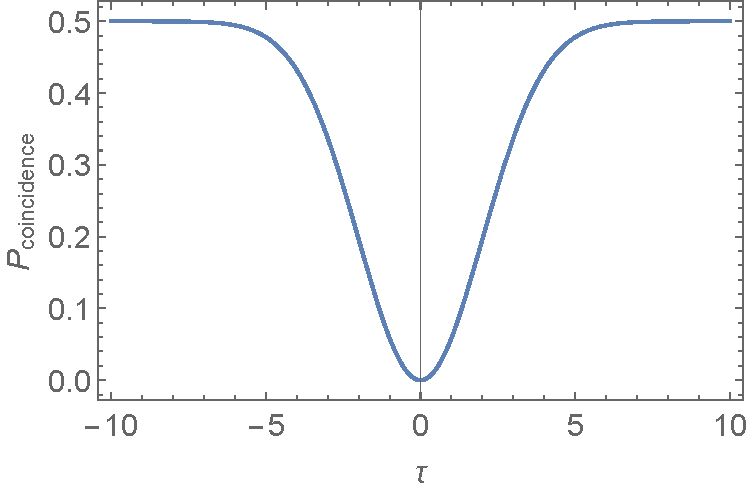
\includegraphics[width=\columnwidth]{HOM_dip}
\caption{Hong-Ou-Mandel dip for two photons with normal Gaussian temporal distribution functions, and temporal offset $\tau$ between them. $\tau$ effectively characterises the degree of photon distinguishability, where \mbox{$\tau=0$} represents complete indistinguishability (quantum statistics), and \mbox{$\tau\to\pm\infty$} represents complete distinguishability (classical statistics). Thus, performing this experiment and measuring $P_\text{coincidence}$ can be used to characterise the degree of photon distinguishability.} \label{fig:HOM_dip}\index{Hong-Ou-Mandel dip}
\end{figure}

In the above representation of mode-mismatch as a temporal or spatial translation, the process is entirely coherent, and could in principle be reversed if the translation were known (which might easily be established using tomographic characterisation techniques). Of course, such translations could occur incoherently also. In particular, `time-jitter' is where this process occurs incoherently, and the photons are subject to probabilistic temporal displacements. In this instance, a pure single-photon state would evolve into a mixture of states subject to different displacements. Since the mode-mismatch is now probabilisitic, it is not reversible. The state of a single photon subject to time-jitter would be of the form,
\begin{align}\index{Time-jitter}
\hat\rho_\text{jitter} = \int_{-\infty}^\infty p_\text{jitter}(\Delta_t) \ket{\psi-\Delta_t}\bra{\psi-\Delta_t}d\Delta_t,
\end{align}
where $p_\text{jitter}(\Delta_t)$ characterises the classical probability distribution of the temporal displacement. Time-jitter is particularly natural in heralded spontaneous parametric down-conversion (SPDC) sources (Sec.~\ref{sec:single_phot_src}), where imprecision in the measurement time of the heralding mode projects that temporal uncertainty onto the heralded state. For this reason, much time is being invested into engineering SPDC sources with separable output photons, such that pathological behaviour of the detection of the heralding photon does not project the heralded photon onto a mixed state. Time-jitter is a major consideration in all present-day single-photon source technologies.

When considering mode-mismatch, there are two general regimes for how it manifests itself in an optical system. The first is when the interference taking place is between distinct, independent photons, i.e HOM interference (or its equivalent generalisations to higher-photon-number systems). The second is when multiple paths followed by a given photon interfere it with itself, i.e Mach-Zehnder (MZ)\index{Mach-Zehnder (MZ) interference} interference. The former only requires mode-matching on the scale of the photons' wave-packets, whereas the latter requires interferometric stability on the order of the photons' wavelength, a far more demanding requirement. This is discussed in greater detail in Sec.~\ref{sec:opt_stab}.

Mode-mismatch has been studied extensively in the context of linear optics quantum computing (LOQC), introduced in Sec.~\ref{sec:KLM_univ}. In particular, it was shown that in the cluster state formalism (Sec.~\ref{sec:CSQC}), mode-mismatch in a fusion gate is equivalent to a dephasing error model, where the dephasing rate is related to the degree of photon distinguishability (i.e visibility) \cite{bib:RohdeRalph06}. More generally, the operation of entangling gates \cite{bib:RohdeFreqTemp05, bib:RohdeGateChar05, bib:RohdeOptPhot05, bib:RohdeTimeRes11} and \textsc{BosonSampling} \cite{bib:RohdeArbSpec15, bib:RohdeArbLow12} have been considered, and explicit error models derived.

%
% Dispersion
%

\subsection{Dispersion} \label{sec:dispersion}\index{Dispersion}

\comment{To do!}

\comment{Discuss dispersion compensation}

%
% Spectral Filtering
%

\subsection{Spectral filtering} \label{sec:spectral_filt} \index{Spectral filtering}

In Sec.~\ref{sec:eff_err} we discussed the loss channel, whereby with some fixed probability photons are lost to the environment. In reality, this process is often not uniform, but frequency-dependent, resulting in spectral filtering effects. For example, optical fibres are typically designed to operate with a particular optical frequency in mind, and will attenuate frequencies outside a given range, implementing, for example, low-pass, high-pass or band-pass spectral filtering.

Because spectral filtering can be regarded as frequency-dependent loss, it can be modelled in the same way as per the loss channel, but using a frequency-dependent beamsplitter with transmissivity $\eta_f(\omega)$, which models the frequency response of the channel. The model is shown in Fig.~\ref{fig:spectral_filter_model}.

\begin{figure}[!htb]
	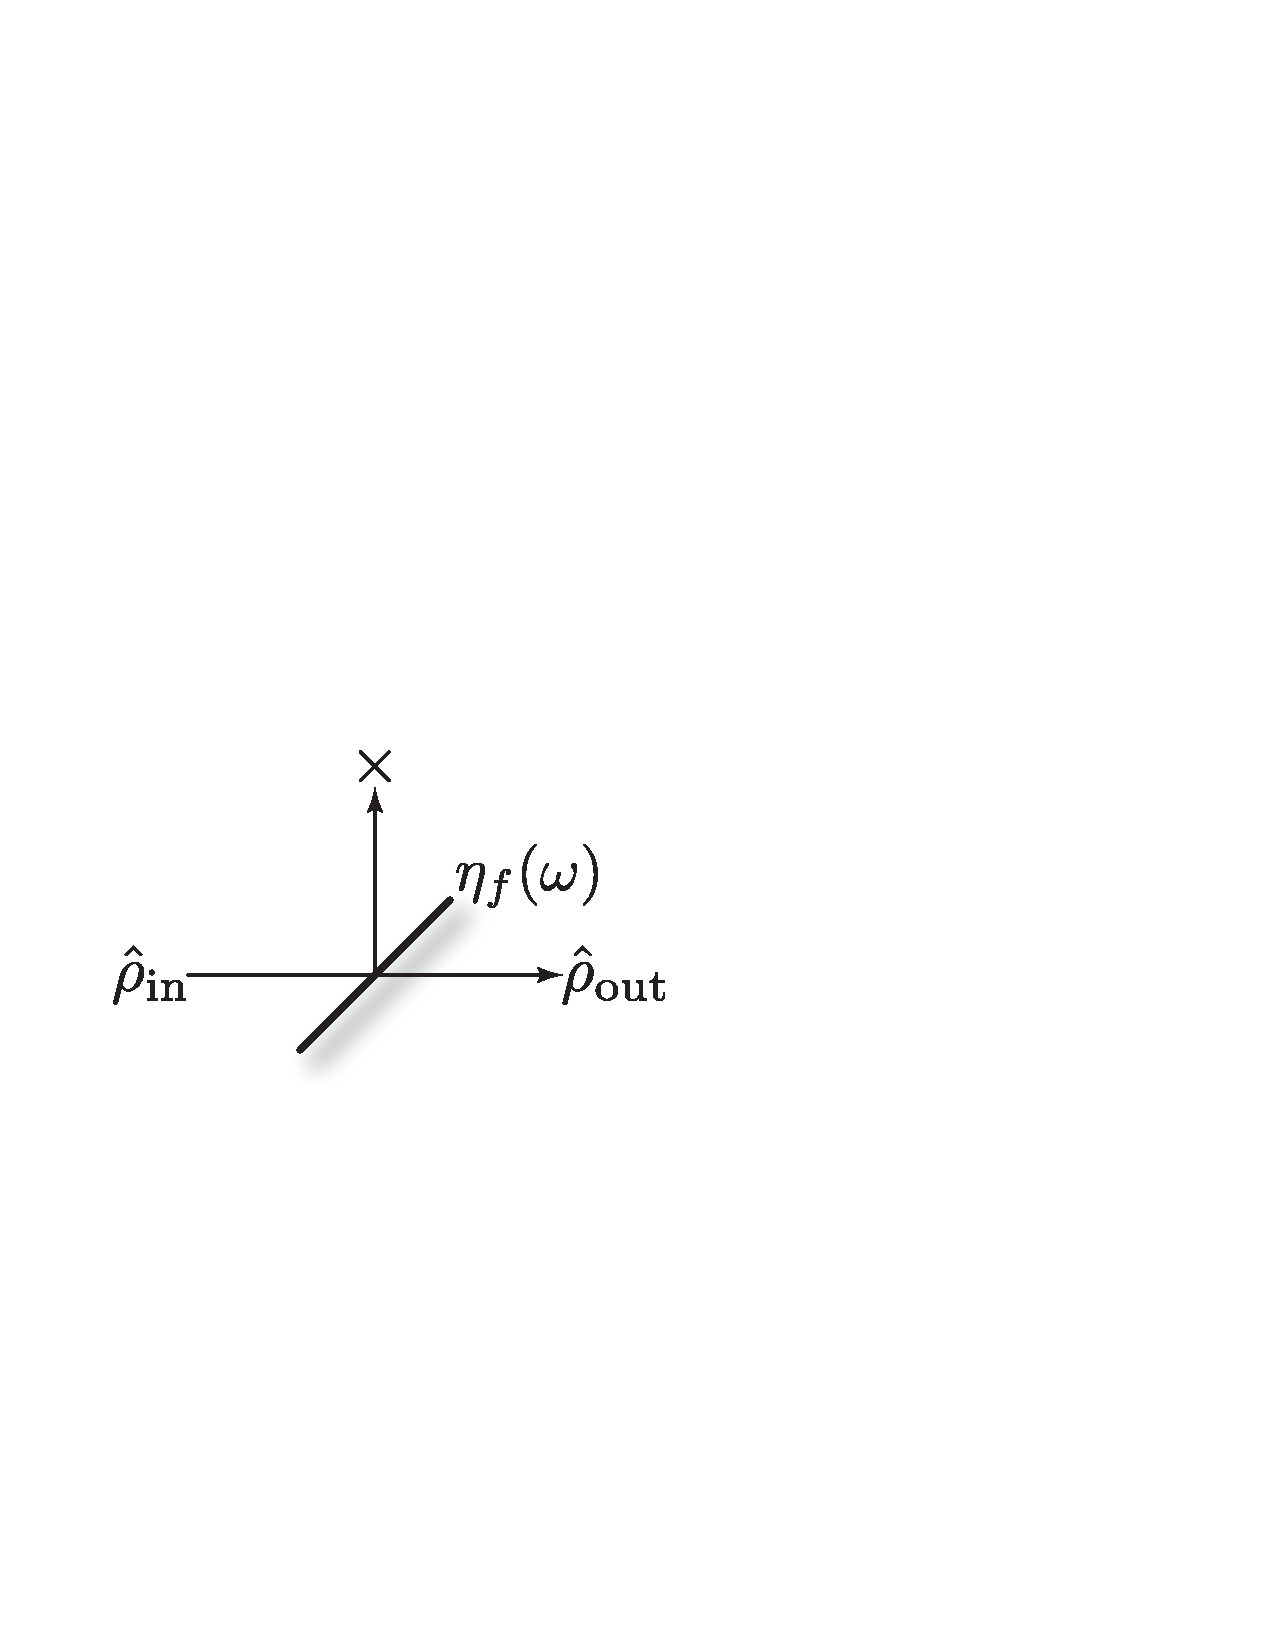
\includegraphics[width=0.5\columnwidth]{spectral_filter_model}
	\caption{Model for the spectral filtering channel. The input state, $\hat\rho_\text{in}$, passes through a beamsplitter of frequency-dependent transmissivity $\eta_f(\omega)$, and the reflected mode discarded, yielding the lossy output state \mbox{$\hat\rho_\text{out} = \mathcal{E}^\text{filter}_{\eta_f}(\hat\rho_\text{in})$}.} \label{fig:spectral_filter_model} \index{Spectral filtering}
\end{figure}

This channel has the effect of modulating the spectral distribution function of a photonic mode operator $\hat{A}_\psi^\dag$ to $\hat{A}_{\psi'}^\dag$, where,
\begin{align}
\psi'(\omega) = \sqrt{\eta_f(\omega)}\psi(\omega).	
\end{align}
Note that unless \mbox{$\eta_f(\omega)=1\,\forall\,\,\psi(\omega)\neq 0$}, the new distribution function $\psi'(\omega)$ will not be normalised, where the normalisation reflects the loss probability,
\begin{align}
p_\text{loss} = 1 - \int_{-\infty}^\infty \eta_f(\omega)|\psi(\omega)|^2\,d\omega.
\end{align}

%
% Phase-Space
%

\subsection{Phase-space} \index{Phase-space errors}

In Sec.~\ref{sec:non_lin_opt} we introduce the displacement and squeezing operations, two non-linear operations which are important ingredients in CV quantum information processing schemes. Of course, such processes are subject to errors.

In the case of the displacement operation, which is implemented by mixing a state with a coherent state on a beamsplitter, errors in the amplitude of the coherent state or in the beamsplitter reflectivity will introduce an offset in the displacement amplitude. Thus, instead of implementing $\hat{D}(\alpha)$, we might over- or under-displace the state, implementing \mbox{$\hat{D}(\Delta)\hat{D}(\alpha)\propto \hat{D}(\alpha+\Delta)$}, for some error $\Delta$.

In the case of the squeezing operation, we might similarly have uncertainty in the squeezing parameter, thus implementing $\hat{S}(\xi+\Delta)$ instead of $\hat{S}(\xi)$.

%
% Costs & Attributes In Quantum Networks
%

\section{Costs \& attributes in quantum networks} \label{sec:quantum_meas_cost}
\index{Costs}\index{Attributes}
As with the classical case in Sec.~\ref{sec:costs}, there will be costs associated with the links and nodes in a network -- nothing is free! In the quantum case, all the usual classical costs are valid, but there are some very important additions of far greater relevance to most quantum applications. Classical digital data is discretised, resulting in data transmission highly robust against noise. In a quantum setting this is necessarily not the case, as the coefficients in quantum superpositions are continuous, meaning that errors accumulate during transmission and states will inevitably deteriorate, unlike digital states. This requires a rethinking of appropriate cost metrics.

%
% Examples
%

\subsection{Examples}

We now briefly introduce some of the key measures for quantifying the quality of quantum communications links, and how they may be expressed as metrics with meaningful operational interpretations. Many of the measures typically employed for characterising quantum systems are not true metrics (i.e costs), but in many cases can be converted to metrics, or used meaningfully as attributes instead.

%
% Efficiency
%

\subsubsection{Efficiency} \index{Loss channel}

The efficiency measure introduced previously is multiplicative, so for consecutive lossy channels the net efficiency is,
\begin{align}
\eta_\text{net}=\prod_i \eta_i,
\end{align}
where $\eta_i$ is the efficiency of the $i$th channel. Intuitively, this is simply telling us that if a photon passes through a channel with success probability $\eta_1$, followed by another with $\eta_2$, the total success probability is \mbox{$\eta_1\eta_2$}.

When employing single-photon encoding of qubits (e.g using the polarisation degree of freedom), there are three basis states of interest: a single photon horizontally polarised ($\ket{H}$); a single photon vertically polarised ($\ket{V}$); and, the vacuum state ($\ket{0}$). The effect of the loss channel on this type of state is to map $\ket{H}$ and $\ket{V}$ to $\ket{\text{0}}$ with probability \mbox{$1-\eta$}, while doing nothing to $\ket{\text{0}}$. Note that because the loss process affects both logical basis states ($\ket{H}$ and $\ket{V}$) identically, its action is invariant under unitary operations in the logical (i.e polarisation) basis space.

%
% Spectral filtering
%

\subsubsection{Spectral filtering} \index{Loss channel}\index{Spectral filtering}

Because spectral filtering can be regarded as a frequency-dependent loss channel, its associated cost can be treated in the same manner, except that rather than keeping track of a single efficiency $\eta$, we track a frequency response function $\eta_f(\omega)$, with the same multiplicative property,
\begin{align}
	\eta_f^\text{(net)}(\omega)=\prod_i \eta_f^{(i)}(\omega).
\end{align}

If we are keeping track of the frequency response, the usual efficiency metric can be made redundant and absorbed into the frequency response function as a uniform response,
\begin{align}
	\eta_f(\omega)=\eta\,\,\forall\,\omega.
\end{align}

%
% Decoherence
%

\subsubsection{Decoherence} \index{Dephasing channel} \index{Depolarising channel} \index{Decoherence}

The dephasing and depolarising channels, given by Eqs.~(\ref{eq:dephasing_channel},\ref{eq:depolarizing_channel}), also behave multiplicatively. If $p_i$ is the probability that the state passing through the $i$th channel in series does not undergo the error process, then the probability of the state passing though the entire series without error is simply,
\begin{align}
p_\text{net}=\prod_i p_i,
\end{align}
exhibiting the same multiplicative behaviour as the loss channel. The same observation applies to any of the other Pauli error channels.

%
% Mode-Mismatch
%

\subsubsection{Mode-mismatch} \index{Mode-mismatch}

In Sec.~\ref{sec:MM_error} we introduced a simple model for temporal mode-mismatch as a displacement in the temporal wave-function of photons propagating through a channel. Clearly, such a process is cumulative -- a temporal displacement of $\Delta_1$ followed by another of $\Delta_2$ yields a net displacement of \mbox{$\Delta_1+\Delta_2$}. Thus, for a chain of such channels we simply accumulate a net temporal displacement of,
\begin{align}
\Delta_\text{net} = \sum_i \Delta_i.
\end{align}

For an incoherent mode-mismatching process, such as time-jitter, an upper bound on the accumulated mismatch may be obtained by summing the maximum temporal displacements at each step.

%
% Distance Measures
%

\subsubsection{Distance measures} \label{sec:fid_metric} \index{Distance measures}

The fidelity of two states directly quantifies how close they are to one another in a geometric sense, i.e on the Bloch sphere \cite{???}, or, in the context of a state passing through a quantum channel, a measure of how well the state is preserved.

The fidelity\index{Fidelity} between two states is defined as,
\begin{align}
\mathcal{F}(\hat\rho_1,\hat\rho_2) = \text{tr}\left(\sqrt{\hat\rho_1^{1/2}\cdot\hat\rho_2\cdot\hat\rho_1^{1/2}}\right),
\end{align}
where,
\begin{align}
& \mathcal{F}(\hat\rho_1,\hat\rho_2) = \mathcal{F}(\hat\rho_2,\hat\rho_1), \nonumber \\
& 0\leq \mathcal{F}(\hat\rho_1,\hat\rho_2) \leq 1.
\end{align}
\mbox{$\mathcal{F}(\hat\rho_1,\hat\rho_2)=1$} iff the states are equal, and \mbox{$\mathcal{F}(\hat\rho_1,\hat\rho_2)=0$} iff they are orthogonal.
In the case where one of the states is a pure state, this simplifies to,
\begin{align}
\mathcal{F}(\hat\rho_1,\ket{\psi_2}) = \bra{\psi_2}\hat\rho_1\ket{\psi_2},
\end{align}
and when both states are pure to simply,
\begin{align}
\mathcal{F}(\ket{\psi_1},\ket{\psi_2}) = |\langle\psi_1 | \psi_2\rangle|^2.
\end{align}

The fidelity is invariant under a common unitary applied to both states,
\begin{align}
\mathcal{F}(\hat\rho_1,\hat\rho_2) = \mathcal{F}(\hat{U}\hat\rho_1 \hat{U}^\dag,\hat{U} \hat\rho_2\,\hat{U}^\dag).
\end{align}

We define the fidelity of two processes, the process fidelity \index{Fidelity} \cite{bib:Gilchrist05}, to be the fidelity between two identical copies of a state that have been evolved under each of those processes, minimised over all possible states. That is, it provides a lower bound on the fidelity between identical states evolved under the two processes. In the context of networking, where quality must be guaranteed, this definition is more appropriate than, say, the average case fidelity. Specifically,
\begin{align}
\mathcal{F}(\mathcal{E}_1,\mathcal{E}_2) &= \min_{\hat\rho} \left[\mathcal{F}(\mathcal{E}_1(\hat\rho),\mathcal{E}_2(\hat\rho))\right] \nonumber \\
&= \text{tr}\left(\sqrt{\chi_1^{1/2}\cdot\chi_2\cdot\chi_1^{1/2}}\right),
\end{align}
\comment{CHECK THIS!} where $\chi_1$ and $\chi_2$ are the process matrices for $\mathcal{E}_1$ and $\mathcal{E}_2$.

The fidelity of two processes is invariant under a common unitary applied to both channels before or after the process. Specifically,
\begin{align}
\mathcal{F}(\mathcal{E}_1,\mathcal{E}_2) &= \mathcal{F}(\mathcal{E}_U\circ\mathcal{E}_1,\mathcal{E}_U\circ\mathcal{E}_2) \nonumber \\
&= \mathcal{F}(\mathcal{E}_1\circ \mathcal{E}_U,\mathcal{E}_2\circ \mathcal{E}_U),
\end{align}
where $\mathcal{E}_U$ is an arbitrary unitary process.

In the special case of an identity channel, $\hat{\mathbb{I}}$, which is of special interest in many communications scenarios, we employ the shorthand,
\begin{align}
\mathcal{F}(\mathcal{E}) = \mathcal{F}(\mathcal{E},\hat{\mathbb{I}}) = \min_{\hat\rho} \left[\mathcal{F}(\hat\rho,\mathcal{E}(\hat\rho))\right].
\end{align}
By definition \mbox{$\mathcal{F}(\mathcal{E})=1$} iff \mbox{$\mathcal{E}=\hat{\mathbb{I}}$}.

A lower bound on the process fidelity of multiple processes in series is multiplicative,
\begin{align}
\mathcal{F}(\mathcal{E}_2\circ\mathcal{E}_1,\mathcal{E}_3) &\geq \mathcal{F}(\mathcal{E}_2,\mathcal{E}_3)\cdot\mathcal{F}(\mathcal{E}_1,\mathcal{E}_3), \nonumber \\
\mathcal{F}(\mathcal{E}_2\circ\mathcal{E}_1) &\geq \mathcal{F}(\mathcal{E}_2)\cdot\mathcal{F}(\mathcal{E}_1).
\end{align}

Generalising to a sequence of $n$ processes in series yields,
\begin{align}
\mathcal{F}(\mathcal{E}_n\circ\dots\circ\mathcal{E}_1) \geq \prod_{i=1}^n \mathcal{F}(\mathcal{E}_i).
\end{align}

An alternate measure for the distance between two quantum states is the trace-norm distance\index{Trace-norm distance}, defined as,
\begin{align}
D(\hat\rho_1,\hat\rho_2) &= \frac{1}{2}\|\hat\rho_1 - \hat\rho_2\|_1 \nonumber\\
&= \frac{1}{2}\sum_i |\lambda_i|,
\end{align}
where $\lambda_i$ are the eigenvalues of \mbox{$\hat\rho_1-\hat\rho_2$}. Like the fidelity, the trace-norm distance is invariant under unitary transformation. Furthermore, it is contractive under the action of quantum processes,
\begin{align}
D(\mathcal{E}(\hat\rho_1),\mathcal{E}(\hat\rho_2)) \leq D(\hat\rho_1,\hat\rho_2).
\end{align}
The trace-norm distance relates to the fidelity according to the following bounds,
\begin{align}
1-F(\hat\rho_1,\hat\rho_2) \leq D(\hat\rho_1,\hat\rho_2) \leq \sqrt{1-F(\hat\rho_1,\hat\rho_2)^2}.
\end{align}
\comment{Add norm for channels}
\comment{Algebraic properties}

%
% Purity
%

\subsubsection{Purity} \index{Purity}

The purity of a state that was initially pure quantifies how well quantum coherence was maintained during evolution, equivalently how well superpositions are maintained. The purity is defined as,
\begin{align}
\mathcal{P}(\hat\rho) = \text{tr}(\hat\rho^2),
\end{align}
where,
\begin{align}
\frac{1}{\text{dim}(\hat\rho)} \leq \mathcal{P}(\hat\rho) \leq 1.
\end{align}
We have \mbox{$\mathcal{P}(\hat\rho) = 1$} iff \mbox{$\hat\rho=\ket{\psi}\bra{\psi}$} is a pure state, and \mbox{$\mathcal{P}(\hat\rho)=1/\text{dim}(\hat\rho)$} iff \mbox{$\hat\rho=\mathbb{\hat{I}}/\text{dim}(\hat\rho)$} is the maximally mixed state.

The purity is invariant under unitary operations,
\begin{align}
\mathcal{P}(\hat\rho) = \mathcal{P}(\hat{U}\hat\rho\,\hat{U}^\dag).
\end{align}

The purity of a process is defined analogously to the fidelity of a process (but only minimising over pure states),
\begin{align}
\mathcal{P}(\mathcal{E}) &= \min_{\ket\psi} \left[\mathcal{P}(\mathcal{E}(\ket\psi))\right] \nonumber \\
&= \text{tr}(\chi^2),
\end{align}
\comment{CHECK THIS!} and as with the fidelity, a lower bound on the purity of multiple processes in series is multiplicative,
\begin{align}
\mathcal{P}(\mathcal{E}_2\circ\mathcal{E}_1)
\geq \mathcal{P}(\mathcal{E}_2)\cdot\mathcal{P}(\mathcal{E}_1).
\end{align}
\comment{CHECK THIS!}. If the channel implements a unitary operation then necessarily \mbox{$\mathcal{P}(\mathcal{E})=1$}.

Like the process fidelity, the purity of a quantum process is invariant under unitary operations,
\begin{align}
\mathcal{P}(\mathcal{E}) &= \mathcal{P}(\mathcal{E}_U\circ\mathcal{E}) \nonumber \\
&= \mathcal{P}(\mathcal{E}\circ\mathcal{E}_U).
\end{align}

Generalising to a sequence of $n$ processes in series yields,
\begin{align}
\mathcal{P}(\mathcal{E}_n\circ\dots\circ\mathcal{E}_1) \geq \prod_{i=1}^n \mathcal{P}(\mathcal{E}_i).
\end{align}

%
% Entanglement
%

\subsubsection{Entanglement} \label{sec:ent_meas} \index{Entanglement measures}

When distributing entanglement between separate nodes, metrics quantifying bipartite entanglement are relevant. For pure bipartite states $\ket{\psi}_{A,B}$, the purity of one of the reduced subsystems directly quantifies the degree of entanglement between them,
\begin{align}
\mathcal{M}(\ket{\psi}_{A,B})) &= \mathcal{P}(\text{tr}_A(\ket{\psi}_{A,B})) \nonumber \\
&= \mathcal{P}(\text{tr}_B(\ket{\psi}_{A,B})),
\end{align}
The entanglement between two systems in invariant under local unitaries,
\begin{align}
\mathcal{M}(\ket{\psi}_{A,B}) = \mathcal{M}([\hat{U}_A\otimes \hat{U}_B]\ket{\psi}_{A,B}).
\end{align}
\comment{What about for processes?}

%
% Phase-Space
%

\subsubsection{Phase-space} \index{Phase-space errors}

Displacements in phase-space accumulate additively, up to a phase-factor. Specifically, the composition of two displacements is given by,
\begin{align}
\hat{D}(\alpha)\hat{D}(\beta) = e^{\frac{1}{2}(\alpha\beta^*-\alpha^*\beta)}\hat{D}(\alpha+\beta).
\end{align}
Thus, the composition of a chain of unwanted or uncertain displacements yields, up to phase, a displacement with amplitude given by the sum of the individual displacement amplitudes.

\comment{To do! What is the composition of multiple squeezing operators? Multiplicative??}

%
% Channel Capacity
%

\subsubsection{Channel capacity} \label{sec:channel_cap} \index{Channel capacity}

The measures considered until now have quantified the preservation of quantum states. Alternately, one might consider information theoretic measures, which quantify the number of bits/qubits transmitted by a link, i.e the number of bits/qubits in common before and after the channel. This is an extremely powerful tool as it upper bounds the amount of information the receiver can extract from the transmitter under \textit{any} measurement scheme, very useful in a cryptographic context, where we want security to be attack-independent.

The Shannon entropy \cite{???} of a classical probability distribution $X$ is given by,
\begin{align}\index{Shannon entropy}
H(X) = -\sum_x p_x\text{log}_2(p_x),
\end{align}
where $p_x$ are the probabilities in the distribution. For a joint distribution over $X$ and $Y$ this simply generalises to,
\begin{align}\index{Joint Shannon entropy}
H(X,Y) =  -\sum_{x,y} p_{x,y}\text{log}_2(p_{x,y})
\end{align}

The von Neuman entropy \cite{???} for quantum density operators, $S(\hat\rho)$, is defined analogously, replacing probabilities with density operator eigenvalues,
\begin{align}\index{von Neuman entropy}
S(\hat\rho) &= - \sum_x \lambda_x \text{log}_2 (\lambda_x) \nonumber \\
&= -\text{tr}(\hat\rho\,\text{log}\,\hat\rho),
\end{align}
where $\{\lambda\}$ is the eigenvalue spectrum of $\hat\rho$. This modification is logically justified, as the eigenvalues can be interpreted directly as a purely classical probability distribution of orthogonal states when the density operator is transformed into a basis with no coherences between basis states (i.e a diagonal basis or spectral decomposition). In that case the Shannon and von Neuman entropies essentially have identical physical interpretations.

The \textit{mutual information} specifies the number of bits in common between two distributions. Equivalently, it is the maximum number of bits that one party can learn about the other. For two classical distributions, $A$ and $B$, this is given by,
\begin{align}\index{Mutual information}
I(A;B) = H(A) + H(B) - H(A,B).
\end{align}
Equivalently, for density operators,
\begin{align}
I(\hat\rho_A;\hat\rho_B) = S(\hat\rho_A) + S(\hat\rho_B) - S(\hat\rho_A,\hat\rho_B),
\end{align}
using the von Neuman entropy. The mutual information between two quantum states is invariant under local unitary transformations,
\begin{align}
I(\hat\rho_A;\hat\rho_B) = I(\hat{U}_A\hat\rho_A \hat{U}_A^\dag; \hat{U}_B\hat\rho_B \hat{U}_B^\dag),
\end{align}
since the eigenvalue spectrum of a density operator is invariant under unitary transformations. Therefore, the mutual information represents the maximum amount of information Bob can learn about Alice's state under \textit{any} local operations.

A quantum process cannot increase the mutual information between two parties. This yields the \textit{data processing inequality} that, for a sequence of channels \mbox{$X\to Y\to Z$},
\begin{align}\index{Data processing inequality}
I(X:Z)&\leq I(X:Y), \nonumber \\
I(X:Z)&\leq I(Y:Z),
\end{align}
with equality if and only if the channel not specified in the identity on the right hand side (\mbox{$Y\to Z$} or \mbox{$X\to Y$} respectively) is unitary, i.e one of the links in the chain perfectly preserves information content.

The mutual information is defined as being between a particular known pair of states. Of course, in a quantum network we will seldom know what the states being communicated are and will therefore be unable to directly calculate the mutual information. To address this, the \textit{classical channel capacity} of a channel is defined as,
\begin{align}\index{Classical channel capacity}
\mathcal{C}(\mathcal{E}) = \max_{\hat\rho} [I(\hat\rho,\mathcal{E}(\hat\rho))],
\end{align}
with the intuitive interpretation as the maximum mutual information between input and output states that can be achieved for the channel. (Note: this definition of `capacity' is not to be confused with that which we later refer to in flow networks).

Analogous to the mutual information for classical systems is the \textit{coherent information} for quantum systems \cite{bib:PhysRevA.54.2629}, defined as,
\begin{align}\index{Coherent information}
I(\hat\rho,\mathcal{E}) = S(\mathcal{E}(\hat\rho)) - S_e(\hat\rho,\mathcal{E}).
\end{align}
\comment{Check up on this coherent information stuff!} Here $S_e$ is the \textit{exchange entropy}, a measure of how much information is exchanged between the state $\hat\rho$ and the environment under the action of the process. Specifically, it is given by the entropy of the environment subsystem in Eq.~(\ref{eq:proc_environment}), after application of the channel. This yields the intuitive interpretation that the coherent information is the information contained in the evolved state, discounted by the amount lost to the environment.

The quantum coherent information exhibits much of the same mathematical structure as the classical mutual information. And analogously, we can define the \textit{quantum channel capacity} as,
\begin{align}\index{Quantum channel capacity}
\mathcal{Q}(\mathcal{E}) = \max_{\hat\rho} I(\hat\rho,\mathcal{E}).
\end{align}

Analytic solutions to $\mathcal{C}(\mathcal{E})$ and $\mathcal{Q}(\mathcal{E})$ are not known even for simple Pauli error channels such as dephasing and depolarisation. However, once net dephasing or depolarisation rates have been calculated across a route, the channel capacities can easily be solved numerically, which is sufficient for the numerical algorithms we will rely upon, where a number representing \textit{cost}, rather than an analytic solution, is all we need.

\comment{Add stuff on channel capacities of different channels, like Pauli error channels etc.}

%
% Latency
%

\subsubsection{Latency} \label{sec:latency_metric} \index{Latency}

Aside from the actual information content of a transmitted quantum state, the latency associated with its transmission is a key consideration in many time-critical applications.

By defining the latency of a link/node as the time between receipt of a quantum state and its retransmission, the total latency of a route is simply the sum of all the individual node and link latencies across the route,
\begin{align}
\mathcal{L}(R) = \sum_{i\in R} \mathcal{L}_i,
\end{align}
where $\mathcal{L}_i$ is the latency associated with the $i$th link in route $R$.

%
% Dollars
%

\subsubsection{Dollars} \label{sec:dollars} \index{Dollar cost}

Not to be overlooked is the actual dollar cost of communicating information. It is unlikely that Alice and Bob outright own the entire infrastructure of particular routes. Rather, different links and nodes are likely to be owned by different operators (particularly in ad hoc networks), who are most likely going to charge users for bandwidth in their network (quantum networks won't be cheap). Clearly dollar costs are additive over the links and nodes within routes,
\begin{align}
\mathcal{C}(R) = \sum_{i\in R} \mathcal{C}_i,
\end{align}
where $\mathcal{C}_i$ is the dollar cost of utilising the $i$th link in route $R$.

%
% Costs as Distance Metrics
%

\subsection{Costs as distance metrics} \label{sec:cost_as_dist} \index{Cost distance metrics}

Def.~\ref{def:metric} defines the properties of a cost metric in the classical context. We now wish to consider this in the quantum context.

If we consider a lossy photonic channel for example, efficiencies ($\eta$) are multiplicative -- for a route \mbox{$v_1\to v_2\to v_3$}, the net efficiency is given by the product of the individual efficiencies, \begin{align}
\eta_{v_1\to v_2 \to v_3} = \eta_{v_1\to v_2} \eta_{v_2\to v_3}.
\end{align}
This is multiplicative rather than additive, clearly not satisfying our definition for a cost metric. However, multiplicative metrics such as this can easily be made additive by shifting to a logarithmic scale, since
\begin{align}
\log(\eta_{v_1\to v_2\to v_3}) = \log(\eta_{v_1\to v_2}) + \log(\eta_{v_2\to v_3}),
\end{align}
which now has a legitimate interpretation as a distance. The same applies to, for example, frequency response functions, which are equivalent to frequency-dependent loss.

In general, for a series of links \mbox{$v_1\to v_2 \to \dots \to v_n$} characterised by multiplicative measure $m$, the equivalent cost metric is,
\begin{align} \label{eq:dist_log}
c_{v_1\to v_2 \to \dots \to v_n} = -\sum_{i=1}^{n-1} \text{log}(m_{v_i\to v_{i+1}}).
\end{align}
We have assumed that \mbox{$0\leq m \leq 1$}, where \mbox{$m=0$} represents complete failure, and \mbox{$m=1$} represents ideal operation.

With these properties, the costs in our graph have an elegant interpretation. In the case of perfect operation, \mbox{$m=1$}, the cost is \mbox{$c=0$}, creating an ideal direct link between neighbouring nodes at no cost. On the other hand for complete failure, \mbox{$m=0$}, the cost metric is \mbox{$c=\infty$}, effectively removing the link from the network and prohibiting pathfinding algorithms from following that route altogether.

Such a logarithmic scale is particularly convenient when a cost metric over links accumulates on a per physical distance basis, in which case the cost metric is simply the physical length of the link multiplied by the metric per unit distance. For example, if a fibre channel implements loss at 3dB/km, the loss over 10km is 10$\times$3dB.

Note that lower bounds on fidelity, purity, efficiency and dephasing are all multiplicative on a scale of 0 to 1, and thus their logarithms may be regarded as cost metrics.

Spatio-temporal mode-mismatch, latency, dollar cost and displacements are clearly automatically metrics as they are additive.

In the case of mutual information and channel capacity, it makes most sense to consider the number of bits that are lost by a channel, rather than the number communicated, since then we have a measure with quasi-metric properties. Specifically, let the number of bits lost by a channel be the difference between the number of bits in the input state and the channel capacity,
\begin{align}
B_\text{lost}(\mathcal{E},\hat\rho) = S(\hat\rho) - \mathcal{C}(\mathcal{E}).
\end{align}
Then there are two cases to consider -- upper and lower bounds on accumulated lost bits.

The best-case scenario is that subsequent channels lose the same bits, giving us a lower bound on the number of lost bits as the maximum number of bits lost by the constituent channels,
\begin{align}
B_\text{lower}(\mathcal{E}_2\circ\mathcal{E}_1,\hat\rho) = \text{max}[B_\text{lost}(\mathcal{E}_1,\hat\rho), B_\text{lost}(\mathcal{E}_2,\hat\rho)].
\end{align}
Alternately, each subsequent channel could lose a different set of bits, in which case the number of lost bits accumulates additively,
\begin{align}
B_\text{upper}(\mathcal{E}_2\circ\mathcal{E}_1,\hat\rho) = B_\text{lost}(\mathcal{E}_1,\hat\rho) + B_\text{lost}(\mathcal{E}_2,\hat\rho). 
\end{align}
Then, the number of actual bits lost is bounded from above and below as,
\begin{align}
B_\text{lower} \leq B_\text{lost} \leq B_\text{upper}.	
\end{align}

%In the case of mutual information, which is not a metric, one can use it to define the \textit{variation of information} metric,
%\begin{align}\index{Variation of information}
%d_\text{VI}(X,Y) &= H(X,Y) - I(X;Y), \nonumber \\
%d_\text{VI}(\hat\rho_A,\hat\rho_B) &= S(\hat\rho_A,\hat\rho_B) - I(\hat\rho_A;\hat\rho_B),
%\end{align}
%or for a channel,
%\begin{align}
%d_\text{VI}(\hat\rho,\mathcal{E}) &= S(\hat\rho,\mathcal{E}(\hat\rho)) - I(\hat\rho;\mathcal{E}(\hat\rho)),
%\end{align}
%which obeys the metric properties.

%
% Non-Trivial Node Operations
%

\subsection{Non-trivial node operations}

Thus far we have considered how to accumulate cost metrics across routes through a network, where each link is subject to some quantum process obeying our notion of a cost metric. But what happens when the links are interspersed with nodes that may be doing more than just simple switching?

A more general scenario to consider is where the nodes are not restricted to routing, but can additionally implement arbitrary unitary operations. This substantially broadens the class of networks under consideration, to encompass nodes capable of doing everything from straightforward routing to entire quantum computations.

All of the examples for cost metrics we introduced in Sec.~\ref{sec:quantum_meas_cost} have the property that they are invariant under unitary operations. Therefore the costs along a route may simply be accumulated as before, summing up the edge weights, without needing any special treatment for node operations, provided they are unitary. For non-unitary node processes, we can merge them into their neighbouring link processes as before (see Fig.~\ref{fig:remove_nodes}).

%
% Quantum Transmission Control Protocol (QTCP)
%

\section{Quantum Transmission Control Protocol (QTCP)} \index{Quantum Transmission Control Protocol (QTCP)}\label{sec:QTCP}

In the classical world, TCP is employed for data transmission and routing. Next we define the quantum equivalent -- the Quantum Transmission Control Protocol (QTCP).

The goal of QTCP is to abstract away the low-level physical operation of a quantum network to create a virtual interface between Alice and Bob, allowing direct access to data as if it were held locally, in much the same way that high-level services like classical FTP facilitate interaction with remote data as though it were a local asset, blind to the intermediate networking.

We consider the scenario where Alice (or a set of Alices) has some state, which she wishes to communicate to Bob (Bobs), with the aim of optimising some arbitrary cost measure. Bob is no guru and doesn't want to concern himself with how the state got from Alice to himself. His only concern is that he receives it and that it satisfies quality constraints he and Alice have agreed upon.

QTCP is the joint software/hardware stack that facilitates these objectives. QTCP begins by logically separating different levels of network functionality into distinct layers of abstraction. The stack is described in detail in Sec.~\ref{sec:prot_stack}. In addition to simple packet switching, the protocol stack is responsible for two very important problems -- routing \textit{strategies} (to be discussed in Sec.~\ref{sec:strategies}), and \textit{collision detection} (Sec.~\ref{sec:collision}). Both of these problems are very low-level in nature, and must be abstracted away by QTCP such that the end-user is oblivious to their operation.

%
% QTCP Protocol Stack
%

\section{QTCP protocol stack} \label{sec:prot_stack} \index{QTCP protocol stack}

As with classical networking, our protocols for quantum networks will be separated into distinct layers, each performing a specific set of tasks with different levels of abstraction.

The structure of the protocol stack for QTCP is shown in Fig.~\ref{fig:stack}. In summary, the layers in the protocol stack are, beginning from the lowest level:
\begin{itemize}
\item \textsc{Data (Message)}\index{Data (message) layer}: Raw data (`payload') Alice wishes to transmit to Bob. Comprises both \textsc{Quantum Data}\index{Quantum data layer} and \textsc{Classical Data}\index{Classical data layer}.
\item \textsc{Packet}\index{Packet layer}: Decomposition of \textsc{Data} into blocks (\textsc{Packet Data}\index{Packet data layer}), and associated classical \textsc{Packet Headers}\index{Packet header layer} containing metadata (e.g routing information).
\item \textsc{Strategy}\index{Strategy layer}: Construct \textsc{Packet} routing strategies based on a cost optimisation algorithm.
\item \textsc{Transport}\index{Transport layer}: Physical routing of \textsc{Packets} to arrive at their destination, based upon metadata contained in \textsc{Packet Header}. Perform collision detection during transit.
\item \textsc{Reconstruction}\index{Reconstruction layer}: Reconstruct \textsc{Data} from received \textsc{Packets}.
\item \textsc{Quality of Service (QoS)}\index{Quality of service (QoS) layer}: Apply QEC and determine whether \textsc{QoS} requirements have been satisfied.
\item \textsc{Services \& Applications}\index{Services \& applications layer}: High-level interface to \textsc{Data} presented to Bob's services and applications. The interface abstracts away lower levels of the protocol stack, presenting Bob with only \textsc{Data} and its associated metadata.
\end{itemize}

\begin{figure}[!htb]\index{QTCP protocol stack}
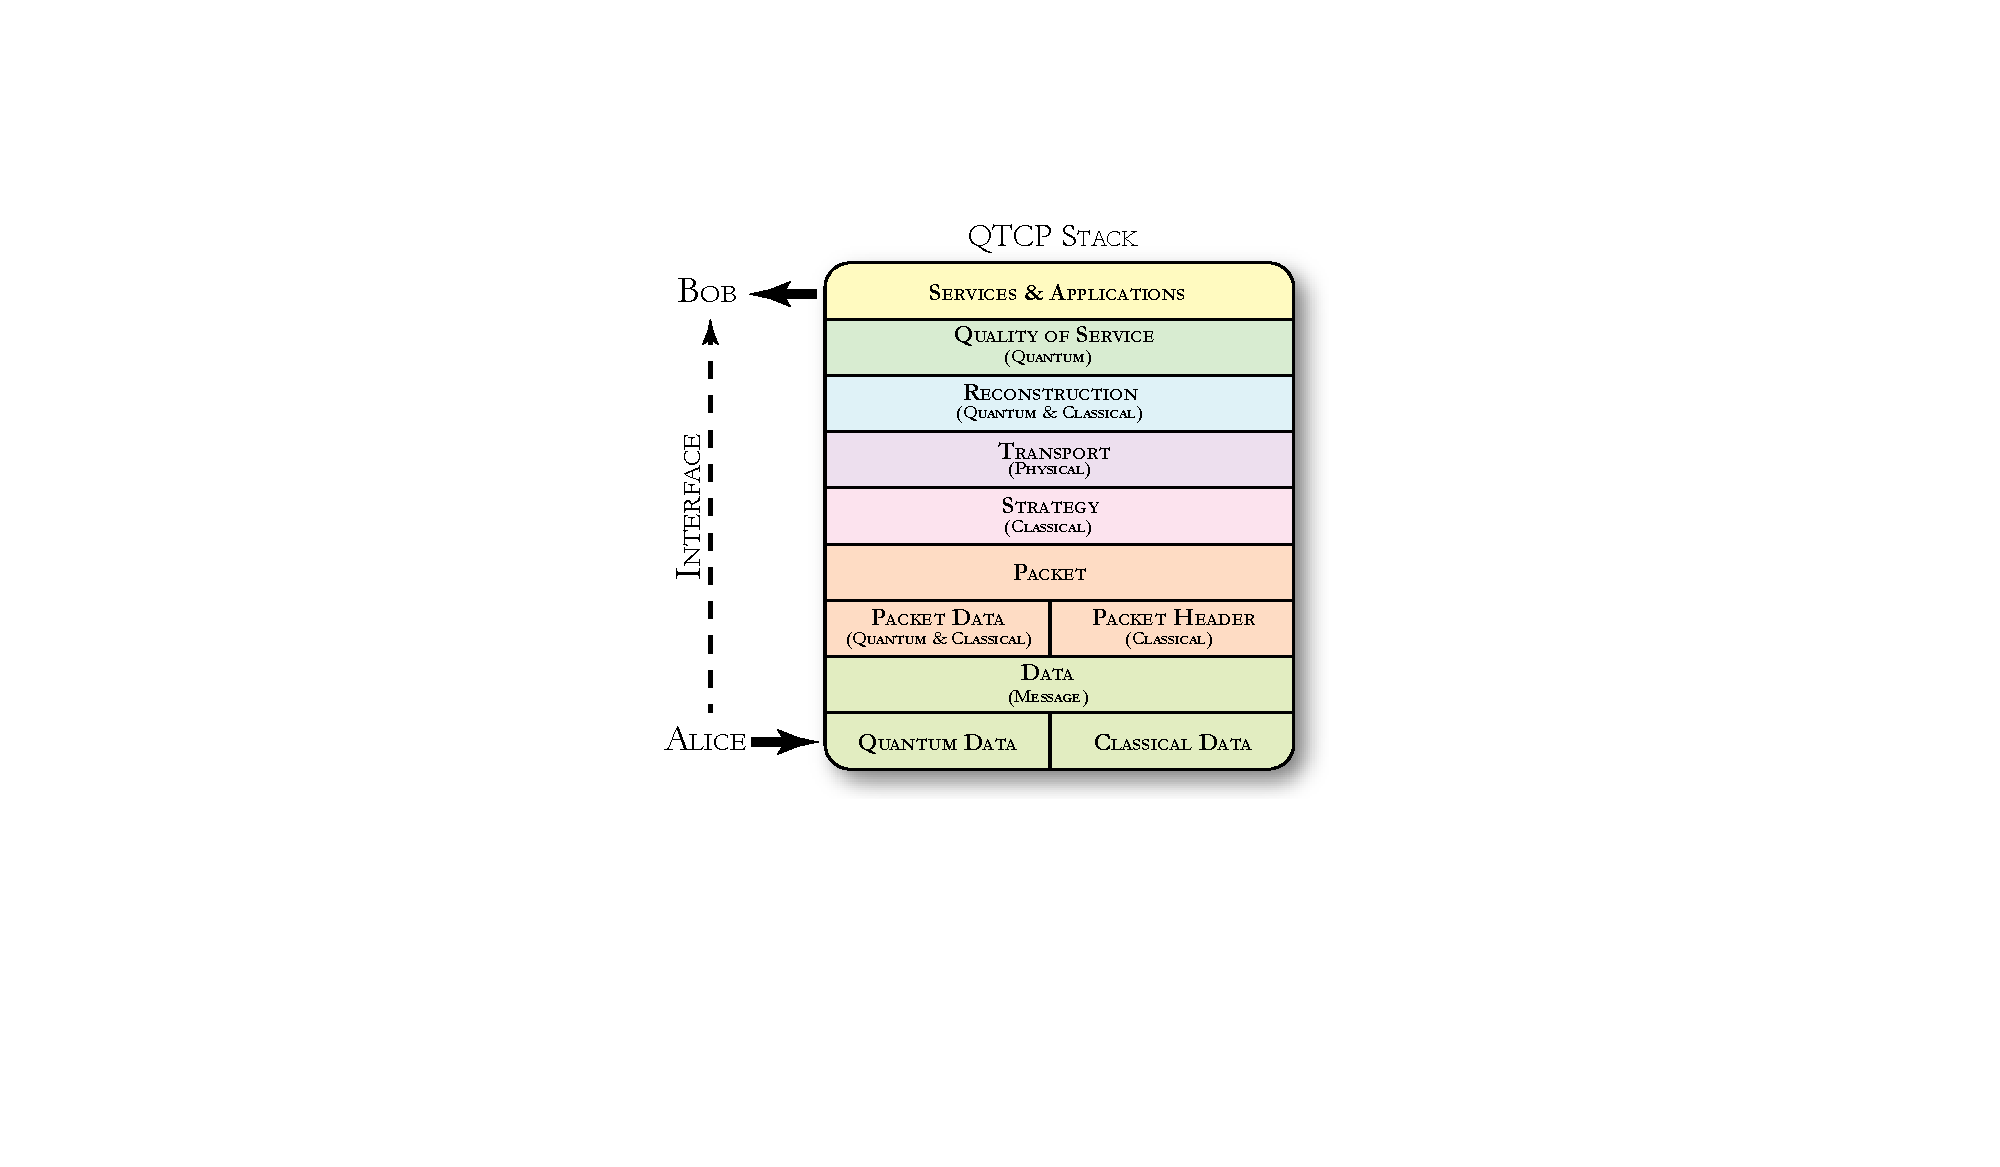
\includegraphics[width=\columnwidth]{stack}
\caption{Protocol stack for QTCP. The protocol stack mediates communication of quantum data from Alice to Bob using the shown layers of abstraction. The end goal is to provide Bob a virtual interface to Alice's transmitted data, while remaining oblivious to the underlying protocol.} \label{fig:stack}\index{QTCP protocol stack}
\end{figure}

Next we describe the operation of these layers in detail.

%
% Data (Message)
%

\subsection{Data (Message)} \index{Data (message) layer}

At the lowest level of the protocol we have the raw \textsc{Data} Alice wishes to communicate to Bob. \textsc{Data} is allowed to comprise both \textsc{Quantum Data} and \textsc{Classical Data} components, and may contain one or the other, or both.

%
% Quantum Data
%

\subsubsection{Quantum data} \index{Quantum data layer}

\textsc{Quantum Data} is allowed to be an arbitrary quantum state. It could be a pure or mixed state, of arbitrary (but predetermined) dimension, or even a subsystem of a larger external state (i.e entangled with another system). We stress that it needn't be expressed using a conventional qubit representation, in the way digital data is necessarily represented using bits. Keep in mind that the quantum internet isn't just there to communicate qubit data streams. Rather, it is intended to act as generally as possible, such that essentially arbitrary \textit{quantum assets}\index{Quantum assets} can be exchanged. These needn't be restricted to any particular type of encoding, such as those discussed in Sec.~\ref{sec:opt_enc_of_qi}. For example, in addition to something `standard' like polarisation-encoded qubits in single photons, one network user might like to share an exotic CV state of light, like a cat state, with his mate whose cat died. Indeed, multiple types of state encoding might be encapsulated within a single \textsc{Packet}. The QTCP acts only as an abstract interface for quantum networking, but is completely blind as to what the underlying data in the network is. QTCP is only concerned with getting that state from Alice to Bob.

%
% Classical Data
%

\subsubsection{Classical data} \index{Classical data layer}

\textsc{Classical Data} is a purely classical state with no coherence (i.e a diagonal density matrix), which may be represented as a classical bit-string. We very intentionally segregate the \textsc{Classical} and \textsc{Quantum} components of \textsc{Data}, since the classical network is expected to be cheaper and more reliable than the quantum network operating in parallel to it. The \textsc{Classical Data} could, for example, provide nodes with classical instructions on what quantum computations to perform on the \textsc{Quantum Data}.

%
% Packet
%

\subsection{Packet} \index{Packet layer}

\textsc{Data} is transmitted as \textsc{Packets}, much in the same way as conventional TCP. The \textsc{Data} is decomposed into three components: \textsc{Quantum Data}, \textsc{Classical Data}, and \textsc{Packet Header}.

We can express the state of an entire \textsc{Packet} as,
\begin{align}
\hat\rho_\text{packet}(i) = \hat\rho_\text{quantum}(i) \oplus \hat\rho_\text{classical}(i) \oplus \hat\rho_\text{header}(i),
\end{align}
where $i$ denotes the $i$th packet. Here $\hat\rho_\text{quantum}$ ($\hat\rho_\text{classical}$) is a block of \textsc{Quantum Block Size} qubits (\textsc{Classical Block Size} bits) taken from the user's \textsc{Quantum Data} (\textsc{Classical Data}), while $\hat\rho_\text{header}$ is the \textsc{Packet's} classical \textsc{Packet Header}. As discussed earlier, since $\hat\rho_\text{quantum}$ is quantum, and $\hat\rho_\text{classical}$ and $\hat\rho_\text{header}$ are classical, they needn't be transmitted together over the same quantum network. Instead all \textsc{Classical Data} and \textsc{Packet Header} could be transmitted over a classical network operating in parallel to and synchronised with the quantum network, which carries the \textsc{Quantum Data}.

Note that while one can always measure classical data without disturbance, this is not the case with quantum data, where measurements cause wavefunction collapse. Thus, while Alice is always able to know $\hat\rho_\text{classical}$ and $\hat\rho_\text{header}$, she may or may not know $\hat\rho_\text{quantum}$. Clearly if she prepared the state herself, she would (hopefully) know what she was doing. But in general, quantum networks could be used for far less trivial networking, where Alice is, for example, an intermediary in a distributed quantum computation. In this instance, Alice is unlikely to know what her \textsc{Quantum Data} is.

%
% Packet Data
%

\subsubsection{Packet data} \index{Packet data layer}

Comprises blocks of both \textsc{Quantum Data} and \textsc{Classical Data}, of sizes \textsc{Quantum Block Size} and \textsc{Classical Block Size} respectively. \textsc{Packet Data} requires that \textsc{Data} be decomposed into distinct subsystems which are independently transmitted by QTCP. For easy of exposition, we will restrict ourselves to the case where the \textsc{Data} is encoded into a stream of qubits (\textsc{Quantum Data}) and bits (\textsc{Classical Data}). But of course other encodings could be used. Also bear in mind that any quantum (classical) information can be encoded into qubits (bits), and once represented as such, the decomposition of \textsc{Data} into \textsc{Packets} arises very naturally and intuitively. The \textsc{Packet's} \textsc{Quantum Data} is what is transmitted via the quantum channels, while the \textsc{Classical Data} is communicated via classical channels.

%
% Packet Header
%

\subsubsection{Packet header} \label{sec:packet_header} \index{Packet header layer}

\textsc{Packet Header} is purely classical and needn't be transmitted over the costly quantum network, instead being transmitted over a complementary classical network, running in parallel to, and synchronised with the quantum network. \textsc{Packet Header} contains no information content from \textsc{Data}, instead comprising only metadata relevant to the higher levels of the protocol stack. In particular, \textsc{Packet Header} contains the following fields:
\begin{itemize}
    \item \textsc{Header Size}\index{Header size}: The number of bits in the \textsc{Packet Header}.
    \item \textsc{Message ID}\index{Message ID}: A unique identifier for the complete message to which this \textsc{Packet} belongs. This field mitigates ambiguity as to which \textsc{Message} this packet belongs when performing \textsc{Reconstruction}.
    \item \textsc{Lifetime}\index{Lifetime}: How long the \textsc{Packet} has been in existence for, i.e since it was initially sent by the \textsc{Sender}. This is used by strategies to prevent collisions.
    \item \textsc{Sender}\index{Sender}: A unique node identifier for the sender (Alice).
    \item \textsc{Recipient}\index{Recipient}: A unique node identifier for the recipient (Bob).
    \item \textsc{Order}\index{Order}: To which block taken from \textsc{Data} does this \textsc{Packet Data} belong? This is extremely important in networks where \textsc{Packets} may arrive out of order. The \textsc{Order} field forms the basis for the \textsc{Reconstruction} layer.
    \item \textsc{Quantum Block Size}\index{Quantum block size}: The number of qubits contained in the \textsc{Quantum} component of \textsc{Packet Data}. This is important for the \textsc{Reconstruction} layer.
    \item \textsc{Classical Block Size}\index{Classical block size}: The number of bits contained in the \textsc{Classical} component of \textsc{Packet Data}, also important for the \textsc{Reconstruction} layer.
    \item \textsc{Routing Queue}\index{Routing queue}: A first in, first out (FIFO) queue of node identifiers, tracing out the entire route for the \textsc{Packet} to follow, in chronological order from the next node to visit all the way to the \textsc{Recipient}.
    \item \textsc{Costs}\index{Costs}: A tuple characterising all the accumulated costs of the \textsc{Packet} at the current stage in the route. These are treated as accumulators that are incremented appropriately after each step, since costs are additive.
    \item \textsc{Attributes}\index{Attributes}: A tuple characterising all the non-\textsc{Cost} properties associated with the \textsc{Packet}. Examples include: the \textsc{Priority} of routing a \textsc{Packet} to its destination; suggesting a preferred routing \textsc{Strategy}; or, indicating whether or not a \textsc{Resend Until Success} protocol may be applied to this \textsc{Packet}.
    \item \textsc{Padding}\index{Padding}: Null data to pad the joint \textsc{Classical Packet Data} and \textsc{Packet Header} fields to be of the same length as the \textsc{Quantum Packet Data}. This ensures that the components of the \textsc{Packet} traversing the quantum and classical channels remain in perfect tandem -- bit for qubit. In Sec.~\ref{sec:transport} we show that this facilitates collision detection without the need to measure quantum states.
    \item \textsc{Checksum}\index{Checksum}: A regular checksum of the entire \textsc{Classical} component of the \textsc{Packet}, including both \textsc{Classical Packet Data} and \textsc{Packet Header}. This also forms a part of the collision detection protocol.
\end{itemize}

One might question why \textsc{Packet Headers} tally accumulated costs when we ought to already know all the costs, since these were employed by the algorithm for choosing strategies in the first case. In the ideal case where all strategies are determined \textit{a priori} and are implemented as intended, this is certainly valid. However, for generality we retain this option since more realistic networks may require dynamically updating strategies during the course of propagation, in which case dynamically tallying costs is appropriate.

%
% Strategy
%

\subsection{Strategy} \label{sec:into_strat} \index{Strategy layer}

Based on the \textsc{Packet Headers} of all users sharing the network, choose routing strategies to optimise cost metrics. The notion of strategies is introduced in Sec.~\ref{sec:strat_opt}, and a detailed discussion of example strategies is presented in Sec.~\ref{sec:strategies}.

Once routings have been determined for all \textsc{Packets}, the \textsc{Routing Queues} in their \textsc{Packet Headers} are initialised accordingly by pushing the sequence of node identifiers tracing out the desired route.

In the case of dynamic, time-dependent strategies, which can be updated within the duration of transmissions, the \textsc{Routing Queues} may need to be updated. A change in a \textsc{Packet's} route simply requires flushing the queue and pushing new node identifiers for each of the nodes in the new route, in chronological order.

The \textsc{Strategy} layer is responsible for evaluating the net cost function $f_\text{cost}$ from Eq.~(\ref{eq:net_cost_R}), which accounts for both \textsc{Costs} and \textsc{Attributes} to calculate a single effective cost measure that may be employed in routing decisions.

%
% Transport
%

\subsection{Transport} \label{sec:transport} \index{Transport layer}

The \textsc{Transport} layer is responsible for actual routing at the physical level, making direct decisions as to what to do with a \textsc{Packet} at each step, based upon the metadata contained in \textsc{Packet Header}, most notably the \textsc{Routing Queue}, which specifies the full route a \textsc{Packet} is destined to follow. It is also responsible for keeping track of costs that accumulate over their route.

Additionally, the \textsc{Transport} layer is responsible for collision detection, whereby multiple packets being transmitted simultaneously over a network interfere with one another, corrupting the data. In classical networking, collision detection is straightforward using checksums. But the usual classical approach breaks down in the quantum setting. In Sec.~\ref{sec:collision} we discuss in detail collision detection in QTCP.

The pseudo-code algorithm implemented by the \textsc{Transport} layer, including collision detection, is shown in Alg.~\ref{alg:transport_alg}.

\begin{table}[!htb]
\fbox{\parbox{0.965\columnwidth}{\texttt{ 
function Transport(Packet):
\begin{enumerate}
    \item nextNode = Packet.RoutingQueue.Pop()
    \item Packet.PhysicallySendTo(nextNode)
    \item Packet.WaitUntilArrivesAt(nextNode)
    \item checksum = Hash(Packet.Header + Packet.ClassicalData)
    \item if(checksum $\neq$ Packet.Header.Checksum) \{
    \setlength{\itemindent}{0.2in}
    \item Packet.Sender.Notify(\textsc{Failure})
    \item Packet.Recipient.Notify(\textsc{Failure})
    \item Packet.Discard()
    \item $\Box$
        \setlength{\itemindent}{0in}
\item \}
    \item Packet.Costs += IncomingLink.Costs
    \item Packet.Attributes.Update()
    \item if(Packet.RoutingQueue.Length = 0) \{
    \setlength{\itemindent}{0.2in}
    \item Return(Packet)
        \setlength{\itemindent}{0in}
    \item \}
    \setlength{\itemindent}{0in}
    \item $\Box$
\end{enumerate}}}}
\caption{Algorithm implemented by the \textsc{Transport} layer of QTCP for each \textsc{Packet}. The \texttt{Attributes.Update()} function is left undefined. This is where arbitrary \textsc{Attribute} dynamics may take place.} \label{alg:transport_alg}
\end{table}

%
% Reconstruction
%

\subsection{Reconstruction} \index{Reconstruction layer}

The \textsc{Reconstruction} layer only serves one purpose -- to chronologically reorder the received \textsc{Packets} based on the \textsc{Order} field in their \textsc{Packet Headers}. This stage is only performed by Bob -- the final recipient -- and not at any intermediate stage. In general this will require Bob to have a quantum memory, able to hold all \textsc{Packet Data} for a sufficient duration as to enable an arbitrary permutation of \textsc{Packets} to be applied, reproducing the correct chronological order.

\begin{table}[!htb]
\fbox{\parbox{0.965\columnwidth}{\texttt{ 
function Reconstruction(Packets):
\begin{enumerate}
    \item Packets.WaitUntilAllReceived()
    \item message = Packets.SortByOrderAscending().data
    \item Packets.Receiver.Notify(message)
     \item $\Box$
\end{enumerate}}}}
\caption{The goal of the \textsc{Reconstruction} layer, is to take a collection of received \textsc{Packets} and reassemble them into the \textsc{Message}.} \label{alg:reconstruction}
\end{table}

%
% Quality of Service (QoS)
%

\subsection{Quality of service (QoS)} \label{sec:QOS} \index{Quality of service (QoS) layer}

In classical networking theory, error detection is an important element of networking protocols. Communication links may be unreliable, or subject to external noise, which users must be able to detect so as to guarantee the quality of their data.

Classically, error detection is typically performed using checksums (hash functions), which generate a short digest of a packet's data that can be recalculated upon arrival to verify integrity. The checksum can be included in the header component of each packet, allowing the remainder of the protocol to remain unchanged.

In the quantum context the elegant notion of checksums is complicated by the fact that calculating a hash function of a quantum state would necessarily entangle the state with the hash function. This would have the undesired effect of causing measurement of the checksum to collapse the quantum state of the data, thereby altering it in an uncontrollable way.

As an alternative to checksums, we could borrow the notion of quantum error correction (QEC)\index{Quantum error correction (QEC)} and fault-tolerance from quantum computing theory \cite{???}. Here we encode a quantum state into a (polynomially) larger Hilbert space. \textit{Syndrome measurements}\index{Syndrome measurements} on some of the states in this larger space allow us to both detect and correct universal error models, such as depolarisation or dephasing, provided that error rates are within the fault-tolerance threshold of the code being employed.

QEC codes have been described for protecting against universal error models, including:
\begin{itemize}
\item Pauli errors: encompassing dephasing, depolarising and amplitude damping \comment{Is A.D a Pauli channel?} error channels.
\item Qubit loss: particularly useful in the optical context where photons are easily lost.
\item Gate failure\index{Gate failure}: essential when gates are non-deterministic, necessarily the case when dealing with maximally entangling two-qubit photonic quantum gates.
\end{itemize}

The first described QEC\index{Quantum error correction (QEC)} code was the 3-qubit code\index{3-qubit code} by \cite{bib:Shor95} for redundantly encoding a single logical qubit into three encoded qubits, allowing the detection and correction of at most a single bit-flip error between the encoded qubits. This protocol is shown in Alg.~\ref{alg:three_QEC}. By switching into a Hadamard-rotated basis, the same code could equivalently correct against at most a single phase-flip error (since \mbox{$\hat{H}\hat{X}\hat{H}=\hat{Z}$}). By concatenating these two codes a 9-qubit code\index{9-qubit code} correcting against a single depolarising error may be implemented.

Since these original ideas into QEC\index{Quantum error correction (QEC)}, countless further codes have been described, able to correct against larger numbers of errors, with far more efficient resource overheads. Currently, topological codes (Sec.~\ref{sec:topol_codes}) are considered the most favourable codes in terms of their elegance, simplicity, high error-correction thresholds, and efficiency in resource overhead. Some such topological codes are particularly enticing, as they can be readily prepared from cluster states (Sec.~\ref{sec:CSQC}), which lend themselves naturally to certain networking methods, such as distributed state preparation.

\begin{table}[!htb]
\fbox{\parbox{0.965\columnwidth}{\texttt{
function ThreeQubitCode($\ket\psi$):
\begin{enumerate}
\item Using two CNOT gates, redundantly encode the logical single-qubit state,
\begin{align}
\ket\psi=\alpha\ket{0}+\beta\ket{1},
\end{align}
into the three-qubit state,
\begin{align}
\ket\psi_R &= \hat{\text{CNOT}}_{1,2}\hat{\text{CNOT}}_{1,3}\ket\psi\ket{00} \nonumber \\
&= \alpha\ket{000}+\beta\ket{111}.
\end{align}
\item Independently apply bit-flip channels $\mathcal{E}_X$ to each of the three encoded qubits.
\item If exactly one bit-flip operation was applied in total, the three possible erroneous encoded states are,
\begin{align}
\ket\psi_1 &= \hat{X}_1 \ket\psi_R = \alpha\ket{001}+\beta\ket{110}, \nonumber \\
\ket\psi_2 &= \hat{X}_2 \ket\psi_R = \alpha\ket{010}+\beta\ket{101}, \nonumber \\
\ket\psi_3 &= \hat{X}_3 \ket\psi_R = \alpha\ket{100}+\beta\ket{011}.
\end{align}
\item Determine the parity of each of the three pairs of encoded qubits.
\item Assuming at most a single bit-flip operation has occurred on the encoded state, the three parity outcomes uniquely determine which encoded qubit the bit-flip was applied to.
\item Apply classically-controlled bit-flip recovery operations, $\mathcal{R}$, to correct the encoded state, recovering $\ket\psi_R$.
\item Apply the inverse of the encoding operation to recover $\ket\psi$.
\item $\Box$
\end{enumerate}}
\begin{align}
\Qcircuit @C=1.3em @R=.6em {
  & \lstick{\ket{\psi}} & \ctrl{2} & \gate{\mathcal{E}_X}  & \qw & \qw              & \ctrl{3}  & \qw       & \ctrl{4} & \qw & \multigate{2}{\ \mathcal{R}\ } & \qw \\
  & \lstick{\ket{0}}    & \targ    & \gate{\mathcal{E}_X}  & \qw & \qw              & \ctrl{2}  & \ctrl{2}  & \qw      & \qw & \ghost{\ \mathcal{R}\ } \qw & \qw \\
  & \lstick{\ket{0}}    & \targ    & \gate{\mathcal{E}_X}  & \qw & \qw              & \qw       & \ctrl{2}  & \ctrl{3} & \qw & \ghost{\ \mathcal{R}\ } \qw & \qw \\
  &          &          &          & & \lstick{\ket{0}} & \targ \qw & \qw       & \qw      & \meter & \control \cw \cwx \\
  &          &          &          & & \lstick{\ket{0}} & \qw       & \targ \qw & \qw      & \meter & \control \cw \cwx \\
  &          &          &          & & \lstick{\ket{0}} & \qw       & \qw       & \targ    & \meter & \control \cw \cwx
} \nonumber
\end{align}
}}
\caption{3-qubit code for protecting against at most a single logical bit-flip error. The doubly-controlled CNOT gates represent parity measurements, \mbox{$n_3=n_1\oplus n_2$}, where $n_i$ represents the value of the $i$th qubit. In a Hadamard-rotated basis, the same circuit may be employed to protect against a single phase-flip error. And by concatenating the two we obtain a 9-qubit code protecting against a single depolarising error, which is a universal error model.} \label{alg:three_QEC}
\end{table}

Different error correcting codes have different error correcting power, and different resource overheads, which must be taken into consideration. The appropriate choice of code will largely be determined by the final \textsc{Services \& Applications} layer. For some simple quantum communications protocols, simple error correction (or even no error correction) may suffice. A full-fledged quantum computation on the other hand will require error rates within a fault-tolerance threshold.

The field of fault-tolerance is already extremely well developed and could be applied directly to QTCP as an abstraction layer directly below the \textsc{Services \& Application} layer of the protocol stack -- the \textsc{QoS} layer -- abstracting it away from the end-user. The transport layer protocol for applying it to the QTCP stack is shown in Alg.~\ref{alg:qos}.

\begin{table}[!htb]
\fbox{\parbox{0.965\columnwidth}{\texttt{ 
function QoS(Packets):
\begin{enumerate}
    \item qec = Packets.ApplyQEC()
    \item if(qec.success = true) \{
    \setlength{\itemindent}{0.2in}
    \item message.Receiver.Notify(qec.data)
    \setlength{\itemindent}{0in}
    \item \} else \{
    \setlength{\itemindent}{0.2in}
    \item message.Receiver.Notify(\textsc{Failure})
    \setlength{\itemindent}{0in}
    \item \}
    \item $\Box$
\end{enumerate}}}}
\caption{QoS algorithm based on any appropriate existing QEC code.} \label{alg:qos}
\end{table}

%
% Services & Applications
%

\subsection{Services \& applications} \index{Services \& applications layer}

Having communicated all the \textsc{Packet Data} from Alice to Bob, performed \textsc{Reconstruction}, and applied \textsc{QoS} protocols, Bob ought to have $\hat\rho_\text{data}$ to a good approximation. The quality of Bob's received state can be inferred directly from the \textsc{Costs} vector contained in the \textsc{Packet Headers}. The final state and its associated quality metrics (\textsc{Costs} and QEC outcomes) may then be provided to Bob as a software interface for end use.

%
% Collision Handling & Classical Errors
%

\section{Collision handling \& classical errors} \label{sec:collision} \index{Collision handling} \index{Classical errors}

In classical networking, protocols such as Ethernet allow users to simply broadcast data at their leisure and rely on \textit{collision detection} to detect when the broadcasts of multiple users have interfered, signalling that both users ought to retransmit following backoff, to minimise the chances of another collision occurring. While this \textsc{Resend Until Success} approach has certainly proven to be effective in classical networking, in a quantum setting the rules of the game are entirely different.

First, collision detection necessarily requires measuring a communications channel to test whether data has been corrupted. Classical networks typically do this by transmitting a checksum with the data, which is recalculated upon arrival for comparison. This raises the obvious problem that quantum measurements are destructive, which means that testing the integrity of our data destroys it in the process -- the last feature we'd like our network to exhibit! However, to overcome this, in Sec.~\ref{sec:transport} we describe a protocol based on the dual classical/quantum network that allows collision detection without measuring quantum states.

Second, collision detection is not always even allowed at all. If one of Alice's packets was entangled with another (i.e she was communicating an entangled system, where the different subsystems resided in different packets), she would not be able to simply retransmit an identical copy of the corrupted packet, since the entanglement with the other system would have been lost and there are no local operations she can do to recover it.

Alternately, Alice might be a part of a distributed computation, where she didn't prepare the data in the first place. In this instance, the no-cloning theorem implies that she cannot, in general, learn what the quantum state was, and therefore would be unable to make a second transmission attempt.

From Alice's point of view, \textsc{Resend Until Success} would clearly work if she was preparing a known state, separable from the other packets. However, collisions on the network caused by her reckless resending would likely corrupt the communications between other parties, leaving them rather ticked off at her.

There are therefore two main approaches to dealing with collisions. First, central planning of all routing could be employed, precisely scheduling all routes \textit{a priori} so as to entirely eliminate any possibility for collisions. Second, if all users in the network were communicating data where packet loss could be tolerated, they could all mutually agree to use the \textsc{Resend Until Success} protocol. This would not require a central authority, and be highly desirable for ad hoc networks. It is important to stress, however, that the latter requires unanimity amongst network participants to function, and the restriction to known, separable states is a major limitation that would prohibit many important uses for quantum networks, such as distributed quantum computation. However, both these approaches are entirely valid in their appropriate context.

In classical TCP all components of data packets are classical and are kept together throughout every stage of transmission. In the quantum case we will instead have a mixture of both quantum and classical data. As mentioned, we will assume that classical communication and computation resources `come for free' (or are at least cheap compared to quantum resources), so there will be a clear disambiguation as to what data is quantum or classical within packets.

As discussed, quantum collision detection is complicated by the fact that measuring quantum data to determine whether it has been corrupted disturbs the quantum state. We address this problem by taking advantage of the duality of the quantum/classical network, discussed in Sec.~\ref{sec:quant_net}. Because the quantum and classical components of the \textsc{Packets} are synchronised and of equal length (thanks to the \textsc{Padding} field of the \textsc{Packet Header}), and because the same applies to all other \textsc{Packets} on the network, a collision in the quantum data necessarily implies a collision in the classical data, and vice versa. Therefore, by applying regular classical collision detection techniques based on checksums (recall \textsc{Packet Header} contains a \textsc{Checksum} field), we can infer collisions in quantum data without actually measuring it. We refer to this as \textit{indirect collision detection}\index{Indirect collision detection}. This guarantees us the ability to detect when a collision has occurred, in which case both quantum \textit{and} classical data are corrupted, or has not occurred, in which case both quantum and classical data are uncorrupted and the quantum data remains unmeasured. Collision detection is incorporated into the pseudo-code implementation of the \textsc{Transport} layer shown in Alg.~\ref{alg:transport_alg}.

This algorithm could, depending upon implementation, be executed locally on the node currently hosting the \textsc{Packet}, or it could be delegated to a central authority, but with the overhead of additional classical communication.

In instances where corruption or loss of packets cannot be tolerated, a more proactive approach may be applied. To preempt the risk of packet collision, one could introduce \textit{probe packets}\index{Probe packets} -- packets containing only classical data, that query a route ahead to negotiate channel usage for the following proper packet, thereby avoiding collisions. Of course, if an upcoming node is unable to guarantee channel capacity immediately, the packet may need to be stored in quantum memory until the channel is available. Thus, it is important to accommodate for this by ensuring that quantum memory is available in nodes preceding links/nodes where collisions are not guaranteed to be mitigated immediately. Quantum memory will be discussed in Sec.~\ref{sec:memory}.

%
% Multi-Packet Operations
%

\section{Multi-packet operations} \index{Multi-packet operations}

\comment{To do}

Thus far we have considered nodes which implement single-packet operations. However, many real-world quantum protocols (to be presented in Sec.~\ref{sec:protocols_quant_int}) will require multi-packet operations, which must be carefully combined in some well-defined way. For example, for state teleportation (Sec.~\ref{sec:teleport}) we must combine a data packet with half of a Bell pair (Sec.~\ref{sec:bell_state_res}). For entanglement swapping (Sec.~\ref{sec:swapping}) -- the essential component in quantum repeater networks (Sec.~\ref{sec:rep_net}) -- two halves of distinct Bell pairs undergo a joint entangling measurement.

To accommodate such multi-packet operations, we must add some modifications to the QTCP protocol to handle:
\begin{itemize}
	\item Packet synchronisation\index{Packet synchronisation}: multiple packets subject to joint operations must be time-synchronised upon implementation of the joint operation. This might involve holding one packet in a quantum memory whilst waiting upon another. Thus, the time required to implement the joint operation is bottlenecked by the packet slowest to arrive.
	\item Bookkeeping of costs and attributes\index{Combining cost \& attributes}: when multiple packets are combined under some operation, how do error costs and attributes accumulate?
	\item Partner packet tracking\index{Partner packet tracking}: packets must keep track of the partner packets with which they are intended to undergo joint operations with. This may be achieved with the addition of {\sc Partners} fields in the packet headers, containing an array of their {\sc Message ID}'s.
	\item Operation signalling\index{Operation signalling}: the recipient node of multiple packets undergoing a joint operation must be informed as to what joint operations should be applied. This may be implemented via the addition of a {\sc What Operation} field to the header.
\end{itemize}

At a high level, these may be implemented in the {\sc Transport} layer as outlined in Alg.~\ref{alg:trans_multi_packet}, where we have intentionally left the functions for combining costs and attributes unspecified. In many instances, the \texttt{CombineCosts()} function could be as simple as a summation of its arguments.

\begin{table}[!htb]
\fbox{\parbox{0.965\columnwidth}{\texttt{ 
function Transport.MultiPacketOperation(packets):
\begin{enumerate}
	\item for(packet$\in$packets) \{
	\setlength{\itemindent}{0.2in}
	\item packet.WaitFor()
	\item packet.HoldInMemory()
	\setlength{\itemindent}{0in}
	\item \}
    \item output = SomeOperation(packets.WhatOperation, packets)
    \item if(output.OperationSuccess = true) \{
	\setlength{\itemindent}{0.2in}
    \item packets.Sender.Notify(\textsc{Success})
    \item output.Costs = CombineCosts(packets.Costs)
    \item output.Attributes = \\
    CombineAttributes(packets.Attributes)
    \item return(output)
	\setlength{\itemindent}{0in}
    \item \} else \{
	\setlength{\itemindent}{0.2in}
    \item packets.Sender.Notify(\textsc{Failure})
  	\setlength{\itemindent}{0in}
    \item \}
    \item $\Box$
\end{enumerate}}}}
\caption{High-level structure of transport layer implementation of multi-packet operations.}\index{Multi-packet operations} \label{alg:trans_multi_packet}
\end{table}

%
% Combining Costs & Attributes
%

\subsection{Combining costs \& attributes} \index{Combining costs \& attributes}

Let us now turn our attention to the details of how the \texttt{CombineCosts()} and \texttt{CombineAttributes()} functions might be implemented. In Sec.~\ref{sec:quantum_meas_cost} we presented a number of examples of prominent costs and attributes that might arise in quantum networks.

To illustrate the basic idea behind this, we now turn our attention to several examples for combining costs and attributes. Some details may vary between specific quantum protocols, although the following typically apply in most general cases.

These ideas logically extend all the way from simple state teleportation to more complicated multi-packet protocols, all the way up to fully distributed quantum computations involving large numbers of qubits and nodes (Sec.~\ref{sec:dist_QC}).

\comment{To do}

%
% Efficiency
%

\subsubsection{Efficiency} \index{Loss channel}

\begin{table}[!htb]
\fbox{\parbox{0.965\columnwidth}{\texttt{ 
function CombineCosts.Efficiency(packets):
\begin{enumerate}
	\item costs = packets.Costs.Efficiency
	\item netCost = sum(costs)
	\item return(netCost)
    \item $\Box$
\end{enumerate}}}}
\caption{Algorithm for combining efficiency metrics in a multi-packet protocol.} \label{alg:combine_eff}
\end{table}

\comment{To do}

%
% Decoherence
%

\subsubsection{Decoherence} \index{Decoherence}

\begin{table}[!htb]
\fbox{\parbox{0.965\columnwidth}{\texttt{ 
function CombineCosts.Decoherence(packets):
\begin{enumerate}
	\item maxDecoherence = \\
    max(packets.Costs.Decoherence)
    \item return(maxDecoherence)
    \item $\Box$
\end{enumerate}}}}
\caption{Transport layer algorithm for combining decoherence rates in a multi-packet protocol.} \label{alg:combine_lat}
\end{table}

\comment{To do}

%
% Latency
%

\subsubsection{Latency} \index{Latency}

In state teleportation there are three channels side-by-side, each exhibiting their own distinct latencies. However, as they are in parallel, the net latency will not be the accumulation of the individual latencies, but rather determined by the largest of those three latencies. That is, the slowest qubit acts as a bottleneck. This is shown in Alg.~\ref{alg:combine_lat}.

\begin{table}[!htb]
\fbox{\parbox{0.965\columnwidth}{\texttt{ 
function CombineCosts.Latency(packets):
\begin{enumerate}
	\item maxLatency = max(packets.Costs.Latency)
    \item return(maxLatency)
    \item $\Box$
\end{enumerate}}}}
\caption{Transport layer algorithm for combining latencies in a multi-packet protocol.} \label{alg:combine_lat}
\end{table}

\comment{To do}

%
% Dollars
%

\subsubsection{Dollars} \index{Dollar cost}

Dollars are perhaps the simplest of costs to account for, as they are simply additive -- the dollar cost of a protocol is the sum of the dollar cost of each component within it. This is shown in Alg.~\ref{alg:combine_dol}.

\begin{table}[!htb]
\fbox{\parbox{0.965\columnwidth}{\texttt{ 
function CombineCosts.Dollars(packets):
\begin{enumerate}
	\item costs = packets.Costs.Dollars
	\item netCost = sum(costs)
	\item return(netCost)
	\item $\Box$
\end{enumerate}}}}
\caption{Transport layer algorithm for combining dollar costs in packet teleportation.} \label{alg:combine_dol}
\end{table}

\comment{To do}

%
% Routing Strategies
%

\section{Routing strategies} \label{sec:strategies} \index{Routing strategies}

In Sec.~\ref{sec:costs} we introduced the notion of network costs, strategies for allocating network resources in Sec.~\ref{sec:route_strats}, and a general formalism for optimising strategies so as to minimise costs in Sec.~\ref{sec:strat_opt}. In this section we present some meaningful example strategies and associated pseudo-code fragments, illustrating the implementation of various aspects of strategies of practical real-world interest.

%
% Single User
%

\subsection{Single user} \label{sec:single_user_shortest} \index{Single user strategies}

Let us begin our discussion of strategies by considering the simplest case of just a single user on the network. Consider the graph shown in Fig.~\ref{fig:simp_route_opt}. This is the same example used earlier, but now the edges have been weighted by some arbitrary cost metric. There are four routes from $A$ to $B$. All have cost \mbox{$c=3$} except the route indicated by the red arrow, which has cost \mbox{$c=2$}. Clearly the latter is optimal in terms of cost minimisation, and any shortest-path algorithm applied between $A$ and $B$ will accurately come to that conclusion. Thus, single-user networks are very trivial to optimise, and there is no distinction between \textsc{Local} and \textsc{Global} strategies.

The very trivial algorithm for this route finding is shown in Alg.~\ref{alg:single_user}, where the \texttt{ShortestPath()} function could be any of the existing, well-known shortest path algorithms (Sec.~\ref{sec:shortest_path}).
\begin{table}[!htb]
\fbox{\parbox{0.965\columnwidth}{\texttt{ 
function Strategy.SingleUser(Packets):
\begin{enumerate}
    \item for(packet$\in$Packets) \{
        \setlength{\itemindent}{.2in}
                \item currentNode = packet.RoutingQueue.Pop()
        \item shortestRoute = \\
        ShortestPath(currentNode,packet.Recipient)
        \item packet.RoutingQueue.Flush()
        \item packet.RoutingQueue.Push(shortestRoute)
    \setlength{\itemindent}{0in}
    \item \}
    \item $\Box$
\end{enumerate}}}}
\caption{For a single user, a simple shortest-path algorithm necessarily finds the optimal route, as there is no potential for packet collisions or competition for network resources.} \label{alg:single_user}
\end{table}

%
% Multiple Users
%

\subsection{Multiple users} \label{sec:two_user} \index{Multiple user strategies}

Next consider the more complex network shown in Fig.~\ref{fig:conflict}. We consider two sender/receiver pairs, \mbox{$A_1\to B_1$} and \mbox{$A_2\to B_2$}. The available routes connecting both pairs overlap, creating competition for network resources.

Let us assume there are just two properties of interest when deciding strategies -- cost in dollars (which may differ for different links), and availability (i.e how many states can the channel handle at once). Let $c_1$ be the dollar cost, and \mbox{$a_1$} be the amount of available channel capacity. Our network is very primitive and each channel can only accommodate one state at a time. Thus, we let \mbox{$a_1=1$} for all links, except for the one common to both $R_1$ and $R_3$, \mbox{($R_1\cap R_3$)}, which we invest more heavily into, since both routes are going to be wanting to use this link.

To define our net cost measure, we combine $c_1$ and $a_1$ according to,
\begin{align}
\mathcal{S} : f_\text{net}(\vec{c}) = \left\{
\begin{array}{l l}
c_1 & \quad \text{if}~ a_1>0 \\
\infty & \quad \text{if}~~ a_1=0 \\
\end{array} \right..
\end{align}
That is, provided bandwidth is available, the link will have the dollar cost $c_1$. If no bandwidth is available, the cost is infinite, thereby removing the respective link from the graph.

Next the cost metrics are updated by the strategy $\mathcal{S}$ following each communication. In this instance this simply decrements the bandwidth attribute for the links that were utilised,
\begin{align}
\mathcal{S} : a_1 \to a_1-1.
\end{align}

Suppose the strategy optimises the \mbox{$A_1\to B_1$} route first, yielding $R_3$, before moving onto the \mbox{$A_2\to D_2$} route. In this case, the reduction of the bandwidth attribute signals that the cheapest route $R_2$ is no longer available to be utilised simultaneously to $R_3$, and must therefore wait its turn on the following clock-cycle. Alternately, the strategy could employ $R_1$ for \mbox{$A_2\to B_2$}, in which case their common link with capacity for two states would eliminate the competition between the two communications, allowing both to take place simultaneously. Thus, there is a tradeoff: for \mbox{$A_2\to B_2$}, we could achieve a net cost of \mbox{$c(A_2\to B_2)=5$}, requiring 2 clock-cycles; or we could achieve simultaneous communication at the expense of increasing cost to \mbox{$c(A_2\to B_2)=6$}. This indicates that when choosing strategies, we must carefully define its goals.

Suppose net cost, rather than clock-cycles, was the key measure of interest. Then choosing the routes $R_1$ and $R_3$ would be the optimal choice. An optimal \textsc{Global} optimisation would recognise this. However, a \textsc{Local} optimisation, based on choosing shortest-paths one-by-by for each sender/receiver pair, may or may not choose the optimal routes, depending on the order in which the decisions were made.

Suppose the \mbox{$A_2\to B_2$} route were optimised first. We would choose $R_2$. Then there would be a traffic jam on the \mbox{$A_1\to B_1$} route, and it would necessarily have to wait its turn. In a time-critical application, where waiting is intolerable, this effectively renders the network useless to the first sender/receiver pair.

If, however, the \mbox{$A_1\to B_1$} were optimised first, choosing $R_3$, then $R_2$ would be prohibited once the bandwidth attributes were updated, and the second best option, $R_1$, would be chosen. Now both communications could take place simultaneously. So we see that the outcomes of \textsc{Local} optimisations needn't always be consistent or unique. Rather, they can be highly dependent upon circumstantial issues, such as the arbitrary order in which routes are chosen for optimisation.

\begin{figure}[!htb]
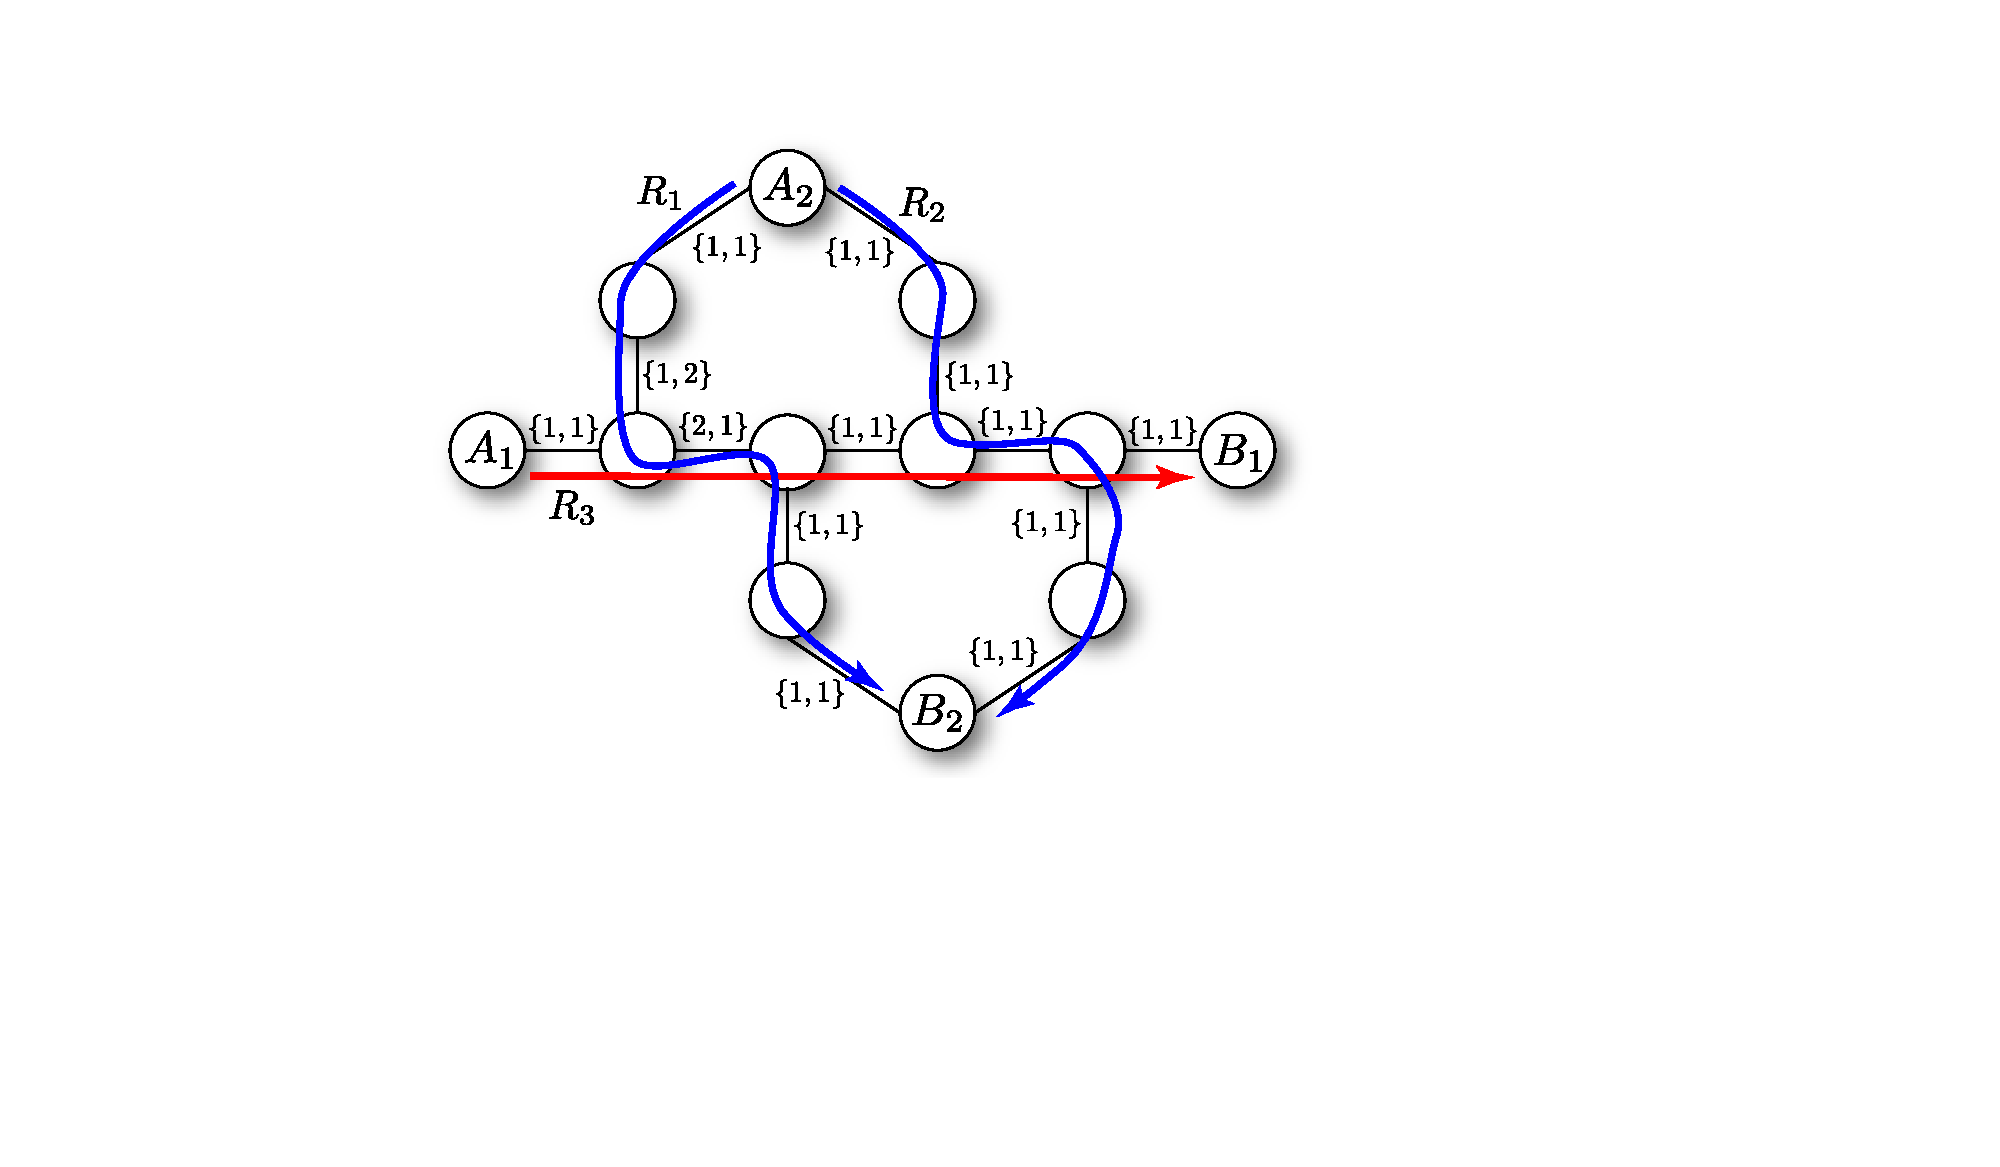
\includegraphics[width=\columnwidth]{conflict}
\caption{A simple network with two competing pairs of senders and receivers, \mbox{$A_1\to B_1$} and \mbox{$A_2\to B_2$}. Edges are labelled by \mbox{$\{b,d\}$}, where $b$ is the bandwidth attribute of the link (i.e number of states that can be communicated simultaneously), and $d$ is the cost metric associated with the link, e.g loss in dB. (blue line) $R_1$ and $R_2$ are two routes from $A_2\to B_2$. Either of these routes could be declared optimal, depending on the choice of cost function. For a trivial additive cost function, $R_2$ would be declared optimal. (red lines) $R_3$ is the optimal route from \mbox{$A_1\to B_1$}.} \label{fig:conflict}
\end{figure}

Generalising this to any number of users is a straightforward extension to the route optimisation problem, incurring a higher computational overhead due to the increased optimisation complexity.

In the upcoming sections we discuss multi-user strategies in more detail. None of these are true \textsc{Global} strategies, but nonetheless address some of the problems facing \textsc{Local} strategies mentioned above.

Truly \textsc{Global} strategies could employ, for example, the vehicle routing problem (Sec.~\ref{sec:VRP}) or vehicle rescheduling problem (Sec.~\ref{sec:VRSP}) algorithms. However, both of these are \textbf{NP}-hard\index{\textbf{NP} \& \textbf{NP}-complete} in general. Thus, the approximation heuristics to be discussed in the following sections are highly applicable.

%
% Round Robin
%

\subsection{Round robin} \label{sec:round_robin} \index{Round robin strategies}

Perhaps the simplest and most elegant multi-user scheduling strategy is to borrow from the idea of time-division multiplexing for preemptive multitasking employed by UNIX operating systems. Here we simply put all live packets in a list, and go through the list, one-by-one, giving each packet an equal time-share of network resources, independent of costs. The algorithm for this is shown in Alg.~\ref{alg:round_robin}.

\begin{table}[!htb]
\fbox{\parbox{0.965\columnwidth}{\texttt{ 
function Strategy.RoundRobin(Packets):
\begin{enumerate}
    \item for(packet$\in$Packets) \{
        \setlength{\itemindent}{.2in}
                \item currentNode = packet.RoutingQueue.Pop()
        \item shortestRoute = \\
        ShortestPath(currentNode,packet.Recipient)
        \item packet.RoutingQueue.Flush()
        \item packet.RoutingQueue.Push(shortestRoute)
    \setlength{\itemindent}{0in} \}
    \item $\Box$
\end{enumerate}}}}
\caption{In the \textsc{Round Robin} strategy we simply iterate through the list of active packets, with no regard for any metrics, or conflicts between them. Rather, we strive for perfect time-sharing equality, and every packet entirely ignores the actions of all other packets.} \label{alg:round_robin}
\end{table}
The \textsc{Round Robin} strategy can be considered base skeleton code for more sophistic algorithms to build upon, simply by reordering the packet queue.

While such a protocol clearly ensures scheduling that gives all packets attention, it is the perfect example of an algorithm subject to the resource allocation imbalance discussed in Sec.~\ref{sec:two_user}. Specifically, the routes being followed by some packets may systemically receive more favourable treatment than others, based on the arbitrary ordering of the list of packets. Also, equal timesharing fails to accommodate for the fact that some routes are inherently more costly than others and deserve a greater share of network resources.

%
% Data Priority
%

\subsection{Data priority} \label{sec:data_priority} \index{Data priority strategies}

Are all men created equal? No. Some packets may inherently be more important than others, and ought to receive priority when allocating network resources. A simple variation on the \textsc{Round Robin} strategy is to, before iterating through the list of packets, order them according to a \textsc{Priority} attribute. Thus, when applying a shortest-path algorithm, it is deemed most important to minimise the costs of the more important packets first.

This is trivially achieved by taking the existing \textsc{Round Robin} strategy, and first ordering the packet list by their priority attributes, i.e by inserting a new line 1, \mbox{\texttt{Packets.SortByPriority()}}.

%
% Randomisation
%

\subsection{Randomisation} \label{sec:random} \index{Randomised strategies}

The imbalance issue facing the \textsc{Round Robin} strategy (Sec.~\ref{sec:round_robin}) may be most trivially addressed using randomisation of the strategy, such that routes are optimised in an order chosen randomly each time. This would allow the different sender/receiver pairs to have equal access to network resources, when averaged over many network uses.

This is also a straightforward variation of the \textsc{Round Robin} strategy, achieved by first randomising the list of packets before the other stages, i.e insert a new line 1, \mbox{\texttt{Packets.RandomizeOrder()}}.

%
% Cost Priority
%

\subsection{Cost priority} \label{sec:cost_priority} \index{Cost priority strategies}

The \textsc{Random} strategy overcomes one key problem facing any \textsc{Local} optimisation strategy. But it is nonetheless merely a mild variation on the \textsc{Round Robin} strategy, guaranteeing equal time-share to each sender/receiver pair. But does equal time-sharing actually represent the best allocation of resources?

It isn't just the order in which routes are chosen, which creates imbalance between users. The costs and attributes of the routes themselves is inevitably biased more in favour of some users than others. To accommodate this we now introduce the \textsc{Cost Priority} strategy. Here, rather than prioritising packets on a random basis, or according to a fixed, predetermined priority attribute, we do so according to their net accumulated cost. Those who have accumulated the highest cost will subsequently be treated with highest priority. This strategy effectively introduces a negative feedback loop into resource allocation, creating a self-regulating (and hopefully stable!) time-multiplexed packet-switched network. The pseudo-code for the \textsc{Cost Priority} strategy is shown in Alg.~\ref{alg:cost_prior_alg}.

\begin{table}[!htb]
\fbox{\parbox{0.965\columnwidth}{\texttt{ 
function Strategy.CostPriority(Packets):
\begin{enumerate}
    \item packetsAndCosts = []
    \item for(packet$\in$Packets) \{
        \setlength{\itemindent}{.2in}
        \item cost = costFunction(packet)
        \item packetsAndCosts.Append([packet,cost])
    \setlength{\itemindent}{0in}
    \item     \}
    \item sorted = \\
        SortByCostDescending(packetsAndCosts)
    \item for(packet$\in$sorted) \{
        \setlength{\itemindent}{.2in}
        \item currentNode = packet.RoutingQueue.Pop()
        \item shortestRoute = \\
        ShortestPath(currentNode,packet.Recipient)
        \item packet.RoutingQueue.Flush()
        \item packet.RoutingQueue.Push(shortestRoute)
    \setlength{\itemindent}{0in}
    \item \}
    \item $\Box$
\end{enumerate}}}}
\caption{The \textsc{Cost Priority} strategy scheduling algorithm that gives highest routing priority to \textsc{Packets} with the highest accumulated cost (i.e which have suffered the most). The as-yet undefined \texttt{costFunction()}, which refers to $f_\text{cost}$ from Eq.~(\ref{eq:net_cost_R}), is where the details of the priority decisions are made, which could be entirely arbitrary. In this example, the shortest route is recalculated at each step, based on the expectation that network metrics are dynamic.} \label{alg:cost_prior_alg}
\end{table}

This is an example of a \textsc{Greedy} optimisation algorithm, which attempts to optimise routing by always optimising the most desperate packets first, in descending order down to the least. It is well-known that \textsc{Greedy} algorithms often do not find global optima. Nonetheless, this approach improves on the previous multi-user protocols.

Let us consider a simple example scenario. Imagine we begin with an ordinary network graph, with edges weighted by costs and attributes. For generality, we will additionally assume the available network resources are very dynamic and unpredictable. The costs associated with links are at the whim of market forces we do not understand (do we ever?). And, for the sake of example, and to make matters worse, the links have been very unreliable lately, and are routinely dropping in and out -- `blackouts'. This effectively rules out \textit{a priori} route optimisation, requiring something dynamic.

There are many users on the network, with many active packets at any give time, but because of the constant oscillations in network resources, some packets have received second-class treatment, and through neglect accumulated an unfair share of state degradation. This simple toy model is, at least qualitatively, something that could arise quite naturally in networks with constrained or unreliable resources.

Let us define an example \textsc{Cost Priority} strategy using the following:
\begin{itemize}
\item \textsc{Latency} cost: How long has the packet has been in transit for? This is actually a very general cost metric, since any other cost metric measured in units per time will be directly proportional to this metric. That is, loss, fidelity, purity, efficiency, and so on, all mirror this metric when expressed on a decibel scale. Of course, the same strategy could have easily been applied to any other cost metric.
\item \textsc{Blackout} attribute: Is our unreliable link actually working right now? A given link will have probability $p_\text{op}$ of being operational at any given time, chosen independently for each link at each clock-cycle. The \texttt{Attributes.Update()} function from Alg.~\ref{alg:transport_alg} is responsible for implementing this.
\item \mbox{\textsc{Cost Function}} ($f_\text{cost}$, \texttt{costFunction()} in Alg.~\ref{alg:cost_prior_alg}): The strategy must make sensible decisions based upon only the above two parameters. Because of the previously mentioned generality of the \textsc{Latency} metric, we would like the net cost to directly reflect this metric, but only of course, if the link is operational. If it is not, then that link must be ruled out entirely by assigning it an infinite cost. Thus, we simply choose,
\begin{align}
\mathcal{S} : f_\text{cost}(c,a) = \left\{
\begin{array}{l l}
c & \quad \text{if}~ a=\text{\texttt{True}} \\
\infty & \quad \text{if}~ a=\text{\texttt{False}} \\
\end{array} \right..
\end{align}
Note that different packets could be associated with different net cost functions, $f_\text{net}$, to accommodate for the different QoS requirements of different users and messages.
\end{itemize}

In other words, the net cost is taken directly from the underlying cost metric, and modulated by an attribute, yielding a net cost for each packet, which is used to determine which packets receive priority.

This provides us with a simple illustration of how costs and attributes can compliment one another to yield meaningful strategies, that improve network performance over na\"ive, but well-intentioned, time-sharing approaches.

%
% All or Nothing
%

\subsection{All or nothing} \label{sec:all_or_nothing} \index{All or nothing strategies}

In some cases, end-user applications may have strict QoS constraints associated with any data they receive. For example, in a time-critical enterprise, say high-frequency trading, receiving information a millisecond too late is worthless, and it would be best to discard the out of date information to free up bandwidth for the next round of information. Alternately, if the fidelity of a state is required to strictly fall within a fault-tolerance threshold, it will be useless if the threshold is violated. In such a context, the \textsc{Strategy} will apply hard boundaries on QoS metrics, discarding anything violating it, after which some other \textsc{Strategy} is applied. The algorithm is summarised in Alg.~\ref{alg:all_or_nothing}.

\begin{table}[!htb]
\fbox{\parbox{0.965\columnwidth}{\texttt{ 
function Strategy.AllOrNothing(Packets, threshold):
\begin{enumerate}
    \item for(packet$\in$Packets) \{
        \setlength{\itemindent}{.2in}
        \item cost = packet.costFunction()
        \item if(cost $\geq$ threshold) \{
        \setlength{\itemindent}{.4in}
            \item packet.Sender.Notify(\textsc{Failure})
            \item packet.Recipient.Notify(\textsc{Failure})
            \item packet.Discard()
                    \setlength{\itemindent}{.2in}
            \item \}
        \setlength{\itemindent}{0in}
    \item \}
    \item Strategy.SomeOtherStrategy(Packets)
    \item $\Box$
\end{enumerate}}}}
\caption{The \textsc{All or Nothing} strategy. If the net cost of a packet exceeds a certain \texttt{threshold}, it is discarded outright, and the sender and recipient notified.} \label{alg:all_or_nothing}
\end{table}

%
% Optimal Flow
%

\subsection{Optimal flow} \index{Optimal flow strategies}

In Sec.~\ref{sec:flow_networks} we introduced flow networks as a means for analysing networks where maximising network flow (throughput) is the primary objective. Formulating our quantum networks in this manner is extremely convenient since, combined with our existing definitions for cost metrics and attributes, we can easily exploit a plethora of known results from flow network theory.

As an example of how load allocation might be applied in a simple network, consider again the network shown in Fig.~\ref{fig:simp_route_opt}, where the edge weights are regular cost metrics (not capacities). Alice wishes to send two packets to Bob, simultaneously if possible. Clearly she would transmit her first packet over the \mbox{$A\to F\to B$} route, since this has lowest cost. But let us assume that every link has a maximum capacity of one packet per unit time. In this case Alice will be unable to send her second packet via the same route and must instead resort to using \mbox{$A\to C \to B$} or \mbox{$A\to D\to B$}. The optimisation is straightforward in this instance. However, in general these types of optimisations are somewhat more involved.

These scenarios are handled by flow network optimisation algorithms, of which there are many. We discuss a few of the most relevant ones for our purposes in Sec.~\ref{sec:graph_theory}. Note that these algorithms are \textsc{Global} optimisation algorithms, requiring complete knowledge of the status of the entire network to perform the optimisation.

The routing strategy is very straightforward, shown in Alg.~\ref{alg:opt_flow}, since the \textsc{Global} flow-optimisation algorithm completely specifies the entire configuration of routes through the network.

\begin{table}[!htb]
\fbox{\parbox{0.965\columnwidth}{\texttt{ 
function Strategy.OptimalFlow(Packets):
\begin{enumerate}
    \item routes = Packets.OptimalFlowRoutes()
    \item for(packet$\in$Packets) \{
        \setlength{\itemindent}{.2in}
                \item packet.RoutingQueue.Flush()
                \item packet.RoutingQueue.Push(routes[packet])
                \setlength{\itemindent}{0in} 
    \item \}
    \item $\Box$
\end{enumerate}}}}
\caption{A generic optimal flow routing strategy. \textsc{Packets} is the array of all packets that ought to be transmitted simultaneously, which are collectively optimised using some flow optimisation algorithm before undergoing transport.} \label{alg:opt_flow}
\end{table}

%
% Extensibility of QTCP
%

\section{Extensibility of QTCP}\index{Extensibility of QTCP} \label{sec:c_vs_a}

In Sec.~\ref{sec:costs} we introduced the notion of the \textit{costs} and \textit{attributes} of links in a classical network, and in Sec.~\ref{sec:quantum_meas_cost} generalised these notions to the quantum case. In Sec.~\ref{sec:packet_header} we described the header format for quantum packets.

The \textsc{Costs} and \textsc{Attributes} fields within the \textsc{Header} are very powerful data structures, implemented as ordered sets of arbitrary dimension, comprising arbitrary data fields. The intention here is to allow QTCP to be extensible into the future, with the addition of new data structures into the protocol. These can be custom designed to, in conjunction with appropriate routing strategies and cost functions, influence the operation of QTCP completely arbitrarily, and easily implement entirely different quantum networking paradigms than presented here.

\textsc{Costs} naturally capture characteristics of the network that accumulate additively along routes, whereas \textsc{Attributes} capture any other characteristics that aren't additive. A network needn't have both costs \textit{and} attributes. It may have one or the other, or both, but not neither, since there must be some measure by which to judge routes.

\comment{To do!}

%
% Scalability
%

\section{Scalability of QTCP}

\comment{To do}

\comment{Discussion of how QTCP protocol/policies might be designed to change with scale. E.g for a small LAN the policies/metrics/attributes might be completely different than for an intercontinental uplink. Discuss how this scalability might be implemented, with examples.}

%
% Message- vs. Packet-Level Routing
%

\section{Message- vs. packet-level routing}

\comment{To do}

\comment{Limit of packet$\to$message size. How does this change strategy.}

%
% Interconnecting & Interfacing Quantum Networks
%

\section{Interconnecting \& interfacing quantum networks} \label{sec:inter} \index{Interfacing quantum networks}

Any global-scale network will inevitably comprise participants choosing to go about things their own way. The physical architecture and medium may vary from one subnetwork to the next, as may the QTCP policies they adopt. The key then is to construct efficient \textit{interconnects} between different levels of the network hierarchy, each of which may subscribe to their own QTCP policies and cross between different physical mediums. Note that the QTCP protocol presented here does not enforce any particular networking policies, but rather provides a high-level framework that can be customised essentially arbitrarily.

For example, the cost metrics and attributes employed at the intercontinental level would most certainly be very different to those in a small LAN. A small LAN might be running applications whereby they can easily reproduce packets and thereby tolerate packet loss. But for a warehouse-scale commercial quantum computing enterprise, responsible for performing one stage of a distributed quantum computation, the loss of a single packet could be extremely costly, requiring the entire computation to be performed completely from scratch due to no-cloning and no-measurement limitations, something that may not come cheaply.

Such interconnects will typically comprise a combination of:
\begin{itemize}
\item Packet switching\index{Packet switching}: such that packets can be arbitrarily switched between the different levels of the network hierarchy.
\item Physical interface: interconnect may be switching between different media. Such physical interfaces have costs associated with them. For example, coupling between free-space and fibre is typically very lossy. Sec.~\ref{sec:opt_inter} discusses optical interfacing with matter qubits, and Sec.~\ref{sec:hybrid} discusses hybrid architectures, where optics mediates entanglement generation between matter qubits.
\item Quantum memory\index{Quantum memory}: such that data can be buffered while it awaits its turn at being switched between networks, as different networks may have different loads and operate at different clock-rates. This is discussed in Sec.~\ref{sec:memory}.
\item Packet format conversion\index{Packet format conversion}: different levels of the network hierarchy may be employing entirely different cost metrics, attributes, and cost functions, requiring packet headers to be reformatted upon switching between networks.
\end{itemize}

The packet switching and quantum memory are implemented as quantum processes at nodes, using the usual quantum process formalism. The physical interface between different mediums, if there is one, could be very diverse, encompassing many types of physical systems, but can always be characterised using the quantum process formalism. Packet headers, which contain all formatting, cost, and routing information are represented entirely classically and communicated entirely by the classical network. Thus, this operation also takes place at nodes, but no quantum processes are taking place.

%
% Network Topologies
%

\section{Network topologies} \index{Network topologies}

As quantum (or classical) networks inherently reside on graphs, it is important to introduce some of the key graph structures of relevance to networking and some of their properties of relevance to quantum networking protocols.

In principle a network could be characterised by any connected graph whatsoever. However, there are certain structures and patterns that emerge very frequently and deserve special attention.

It is paramount that QTCP protocols have the capacity to deal with the diverse network topologies that are likely to present themselves in the future real-world quantum internet. Some of the graph-theoretic algorithms that we rely on in our QTCP protocol (Sec.~\ref{sec:graph_theory}) are computationally efficient for \textit{arbitrary} graph topologies, even more so for certain classes of graphs exhibiting particular structure, such as tree graphs or complete graphs. Others, however, are computationally inefficient in general, but may have efficient approximation algorithms for some or all classes of topologies.

We will now review some of the graph structures most likely to arise in quantum networks.

%
% Point-To-Point
%

\subsection{Point-to-point (P2P)} \index{Point-to-point (P2P) topologies}

The most trivial network topology, which also acts as the elementary primitive from which our other topologies will be constructed is a simple dedicated point-to-point (P2P) connection between two parties, where the sender and recipient of a packet reside on neighbouring nodes.

Such P2P connections may be reserved exclusively for the two connected neighbouring nodes. In this instance, the packets' \textsc{Routing Queue}s trivially specify just the recipient. Alternately, the P2P link may be an intermediate step between more distant sender/recipient pairs.

In the case whereby the P2P connection is reserved exclusively for a particular sender/recipient pair, the link has the property that there is no competition between multiple users sharing the channel, and the QTCP stack needn't concern itself with dynamic routing strategies\footnote{Assuming the P2P channel has sufficient capacity to meet demand and exhibits better cost metrics than other potential redundant, indirect routes.}. This significantly simplifies network scheduling algorithms (Sec.~\ref{sec:strategies}), and a \textsc{First-Come First-Served} (i.e chronologically ordered FIFO queue) strategy may be employed. Furthermore, packet collisions cannot occur, thereby improving network efficiency.

In the case whereby the P2P connection is not reserved for exclusive use between a single sender/recipient pair, but shared between different competing routes in the network, the importance of network routing strategies manifests itself. Now competition for access to the channel will reduce network efficiency, scaling inversely against the number of network participants, and the priorities and costs of packets must be tallied for the purpose of implementing routing strategies.

%
% Complete
%

\subsection{Complete} \index{Complete topologies}

The complete graph, denoted $K_{|V|}$, is a $|V|$-vertex graph where every vertex has an undirected link to every other. From a networking point of view, this can be regarded as the extremity of exclusive-use P2P networking, whereby every node has a direct link with every other. Thus, any sender can directly communicate with any receiver, via a dedicated direct channel, with no need to utilise any indirect routes. This topology has the favourable property that although any node can communicate with any other, by exclusively utilising direct P2P links we achieve several benefits:
\begin{itemize}
\item Packet collisions can be mitigated entirely, thereby maximising network efficiency.
\item Competition for the use of links can be eliminated, minimising congestion and the need for buffering (i.e quantum memory).
\item Network costs can typically be minimised, as every route only traverses a single link, and there will be no accumulation of costs.
\item The network has maximal route redundancy, making it the most tolerant against link failures\footnote{To disconnect a given node from the network, all \mbox{$|V|-1$} links emanating from it must be broken, otherwise redundant routes to the remainder of the network will exist.}.
\item A trivial \textsc{First-Come First-Served} routing strategy can be employed, eliminating the need for any dynamic or computationally complex strategies.
\item If the network allows indirect routes to be established, the maximal redundancy of the topology also maximises the ability for routing strategies to engage in load-balancing across routes.
\item In the special case of a symmetric complete graph, whereby all edge weights are approximately equal, the shortest path between any two nodes is trivially the P2P link between them, and no complex scheduling algorithms are required.
\end{itemize}
However, these highly desirable benefits come at the expense of requiring the most elaborate and expensive network, with maximal interconnectedness.

This type of topology could arise in, for example, international-scale networks, where links of very high bandwidth (and value) between nations or continents need to be maximally utilised, which would be undermined by sparse, shared network topologies. Additionally, in this instance route redundancy will be highly valued, as the isolation of one continent from another would be catastrophic to the functioning of the global network.

Fig.~\ref{fig:complete_graph} illustrates the $K_{15}$ graph. The number of edges scales as $O(n^2)$. Clearly route-finding is trivial, since there is always a direct link from sender to receiver, with no possibility of collisions with other packets, requiring $O(1)$ search time (assuming all users are communicating only via their direct links with one another, which may not strictly be the case when costs are factored into strategies).

\begin{figure}[!htb]
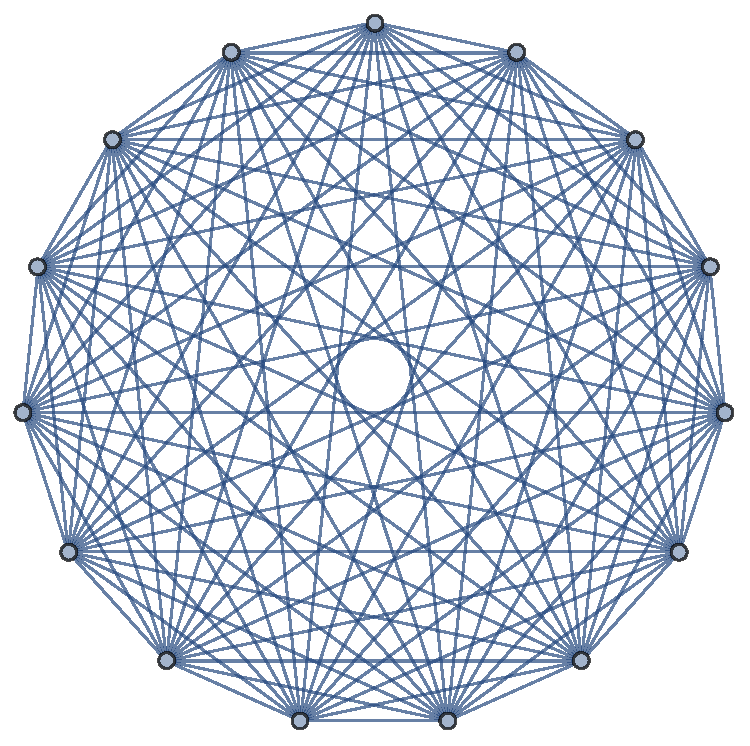
\includegraphics[width=0.7\columnwidth]{K_15}
\caption{The 15-vertex complete graph, $K_{15}$. Every vertex has an edge to every other, with a total of 105 edges.} \label{fig:complete_graph}
\end{figure}

%
% Lattice
%

\subsection{Lattice} \index{Lattice topologies}

A lattice graph is simply an \mbox{$n\times m$} lattice of vertices (of any geometry, e.g squares), connecting each vertex to its immediate geometric neighbours. This type of graph is useful when link costs are measured in terms of Euclidean distances, and nodes have nearest neighbour links. An example is shown in Fig.~\ref{fig:lattice}.

\begin{figure}[!htb]
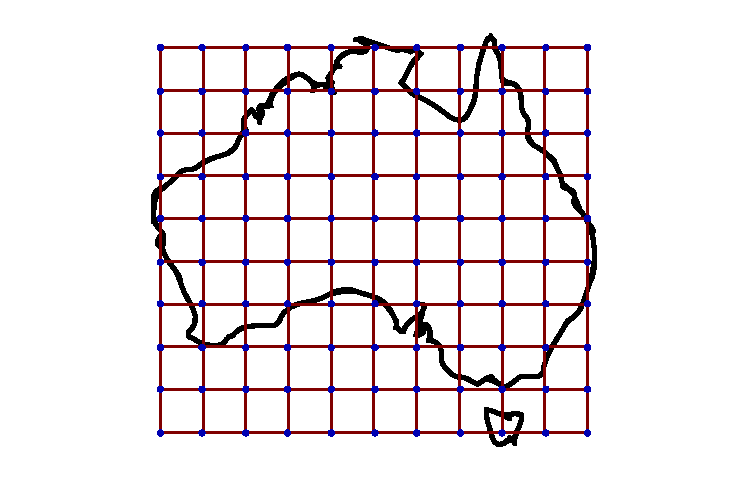
\includegraphics[width=0.7\columnwidth]{lattice}
\caption{A \mbox{$10\times 11$} square lattice graph, and how it might represent a network topology with geographically associated costs. Notice that Hobart has no internet connection (why even include Tasmania at all?).} \label{fig:lattice}
\end{figure}

A slightly distorted lattice graph, in which vertices have been dragged around geometrically to match, for example, cities within a country, closely resembles the topology of the network. Similarly, if the nodes represent houses in the street layout of a highly regular city like Manhattan, a lattice may be a good approximation.

In the case of a balanced lattice, in which all edges are of equal weight, the cost of a route is the sum of the number of steps in the vertical and horizontal directions, also known as the Manhattan or $L_1$ distance,
\begin{align}
L_1 = |x_\text{start} - x_\text{finish}| + |y_\text{start} - y_\text{finish}|.
\end{align}
In this case, route finding is simplified, since \textit{all} routes, which strictly traverse in one direction vertically and one direction horizontally, are optimal and of equal distance.

%
% Tree
%

\subsection{Tree} \label{sec:tree_graph} \index{Tree topologies}

A tree is a graph containing no cycles, only \textit{branches}. There are many uses for tree graphs, but one property is of particular convenience in many applications: because the graph is acyclic, there is always exactly one path from any vertex to any other. This mitigates the need for shortest-path algorithms designed for general graphs, and simplifies route-finding algorithms (to be discussed in Sec.~\ref{sec:path_exp}). However, this brings with it the drawback that the topology is most vulnerable to link failures, since the removal of any link from the tree will separate it into a bipartite graph, making communication between the two disjoint subgraphs (which are also trees) impossible, as there are no redundant routes. In a sense, tree graphs can be considered the polar opposites of complete graphs.

Trees are specified entirely by \textit{branching parameters} ($b_i$) -- the number of child nodes emanating from a given node, $i$. In general, branching parameters may be distinct for each node, although often trees with symmetries in their branching structures are considered, such as the balanced trees discussed in Sec.~\ref{sec:bal_tree}. A node terminates a branch if its branching parameter is zero (i.e it has no children).

The \textit{depth} ($d$) of a tree is the maximum number of steps from the root node to a terminating node with no children. The depth scales between \mbox{$d=O(|V|)$}, for the trivial linear tree (\mbox{$b_i=1$}), and \mbox{$d=O(\text{log}|V|)$} for non-trivial branching parameters (i.e \mbox{$b_i\neq 1$}).

The worst-case number of edges that must be traversed to reach any vertex from any other is $2d$, which implies that accumulated cost metrics scale as at most \mbox{$c=O(|V|)$}. Trees are the most frugal graphs in their number of edges, which are fixed at \mbox{$|E|=|V|-1$}, irrespective of the branching parameters, since because the graph is strictly acyclic, every addition of an edge requires the addition of exactly a single vertex. This makes tree graphs the cheapest to construct in terms of physical resource usage.

%
% Balanced Tree
%

\subsubsection{Balanced tree} \label{sec:bal_tree} \index{Balanced tree topologies}

A balanced tree is a tree with a regular, self-similar structure, in which every node at a given depth is the parent of the same number of sub-nodes, all separated by the same edge weights. That is, the network has a hierarchical structure, subdividing into identically structured subnetworks. Such a network is characterised by just two parameters -- the branching parameter, $b$, and the depth, $d$. Some examples of balanced trees with different $b$ and $d$ are shown in Fig.~\ref{fig:tree_example}.

\begin{figure}[!htb]
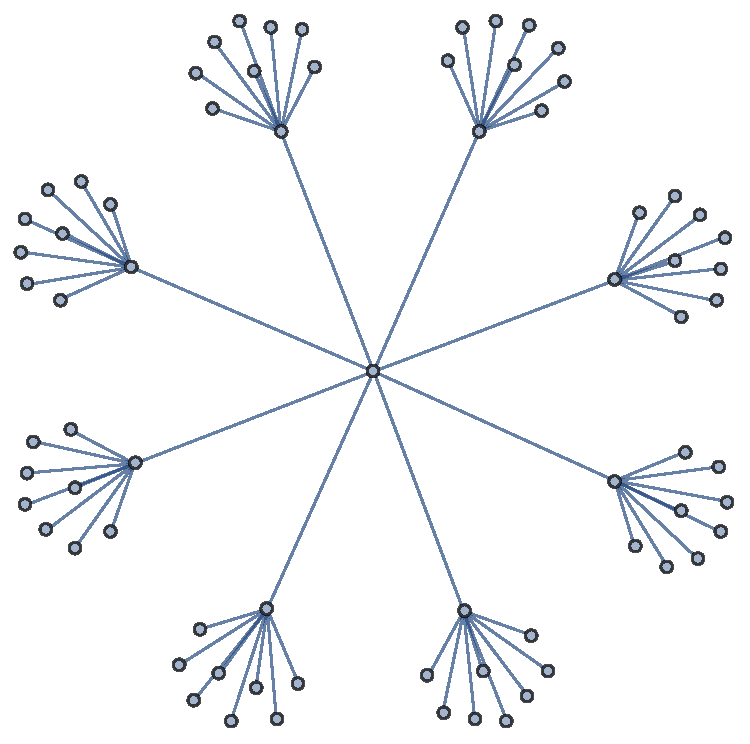
\includegraphics[width=0.75\columnwidth]{tree_3_8} \\
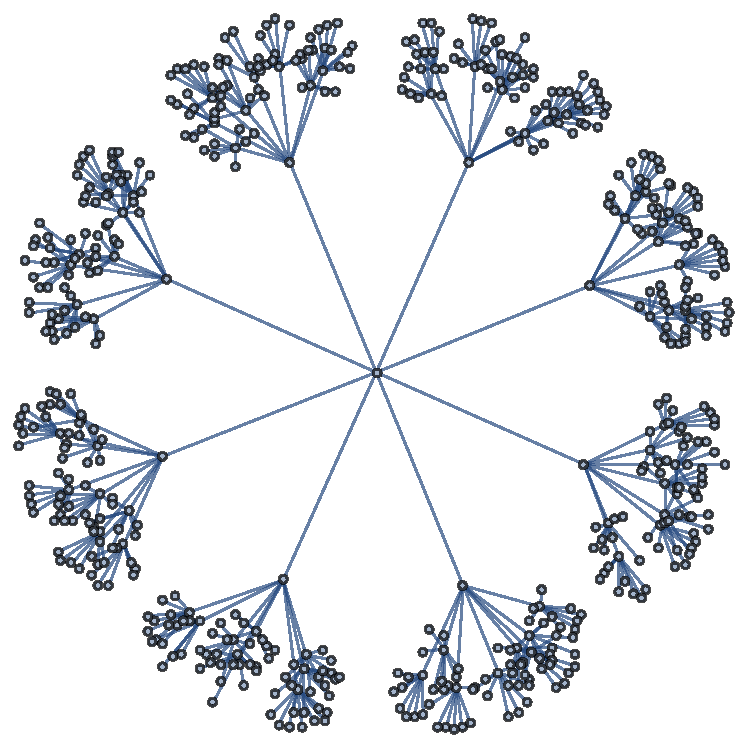
\includegraphics[width=0.75\columnwidth]{tree_4_8} \\
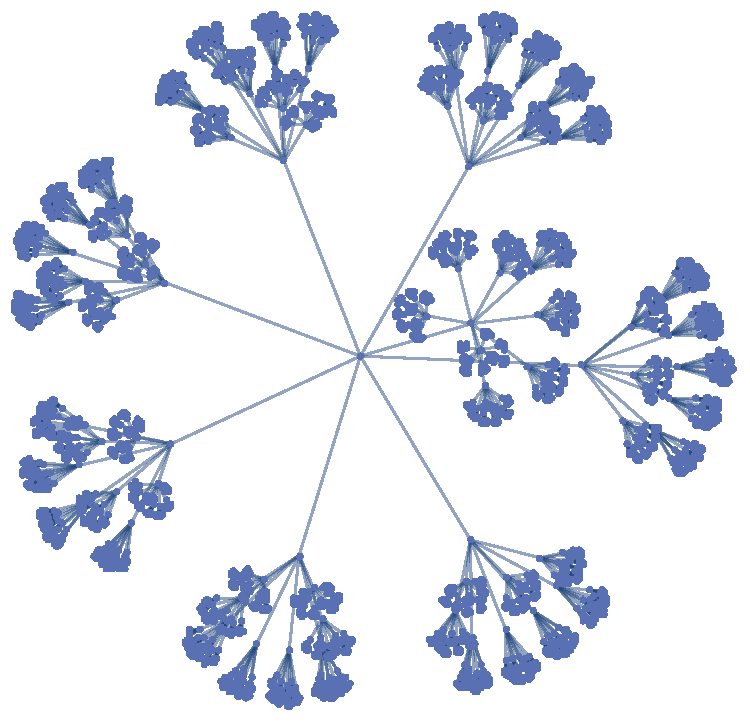
\includegraphics[width=0.75\columnwidth]{tree_5_8}
\caption{Balanced tree graphs with branching factor $b=8$, and depths $d=3,4,5$ (top to bottom). Despite having no redundant paths, the hierarchical structure of balanced trees somewhat resembles that of real-world networks, which are typically decomposed into a pyramid scheme of progressively smaller subnetworks.} \label{fig:tree_example}
\end{figure}

This type of structure is (approximately) natural in many realistic scenarios. Consider for example a network containing a hierarchy of clusters of nodes representing a LAN, followed by a neighbouring internet router, followed by a city-wide router, followed by a country-wide router. In such a case, this type of general structure is typical (although more realistically one might expect the branching parameter to vary with depth).

A special case is when \mbox{$d=1$}, which we refer to as a \textit{star} graph. This might arise naturally when a series of subnets are connected together via a central router (e.g Fig.~\ref{fig:net_hierarchy}), with no further hierarchy in the network.

%
% Random Tree
%

\subsubsection{Random tree} \index{Random tree topologies}

While balanced trees accurately capture the hierarchical nature of realistic networks, they are somewhat contrived in their perfect symmetry. The subnetworks in a given network are not likely to actually all be identical. Random trees are perhaps more realistic, in that their tree structure captures the hierarchical nature of real-world networks, and also their highly ad hoc nature.

To construct a random tree we simply randomly choose a branching parameter, according to some arbitrary distribution, for every node. When a node has \mbox{$b_i=0$}, it terminates the lineage. Some examples of random trees are shown in Fig.~\ref{fig:random_tree}.

\begin{figure}[!htb]
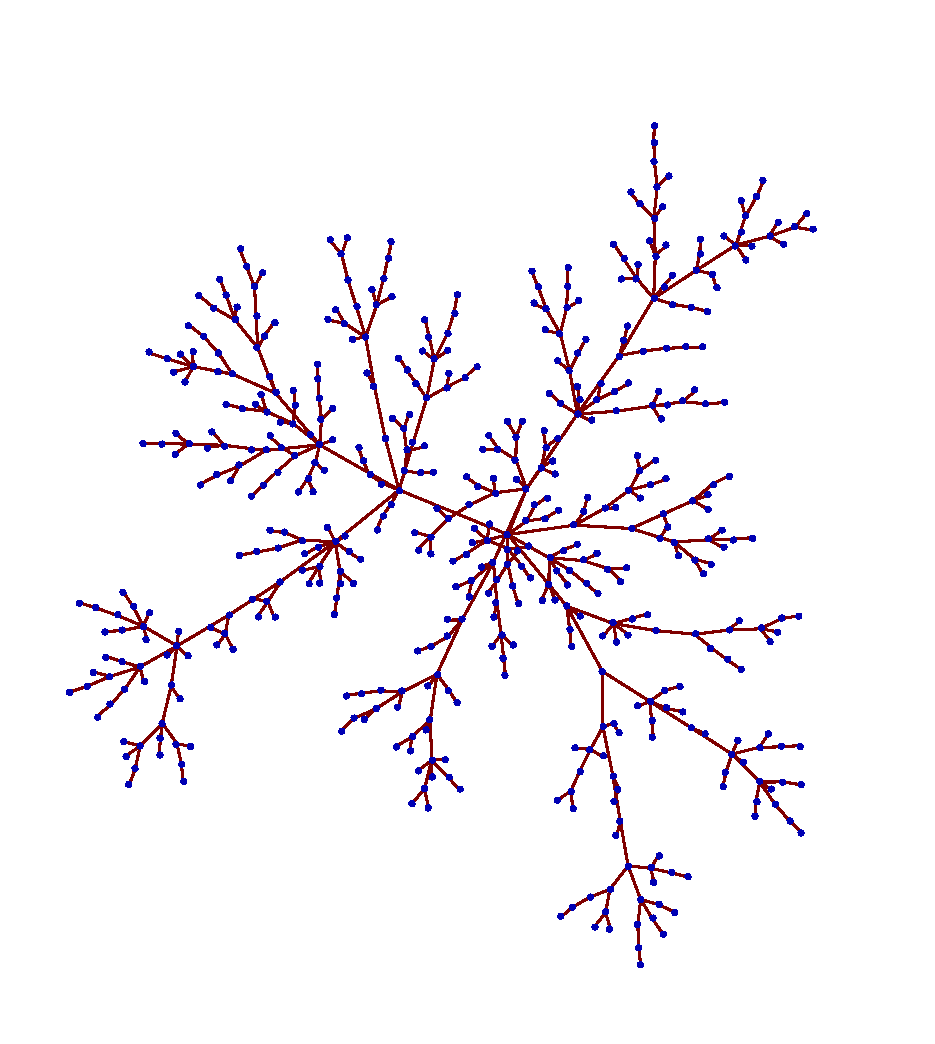
\includegraphics[width=\columnwidth]{random_tree_1} \\
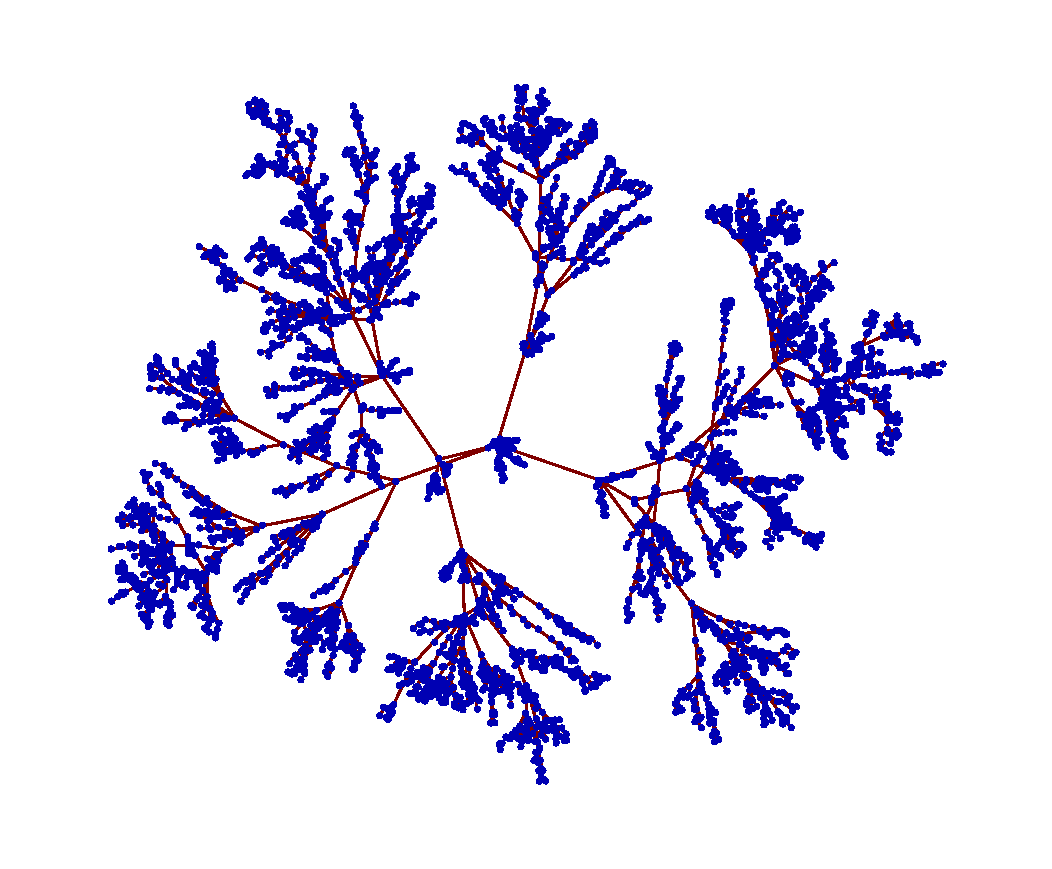
\includegraphics[width=\columnwidth]{random_tree_2}
\caption{Random trees with different randomised branching parameters (higher $b$ at bottom). When a node has zero branches, it terminates the branch. This type of graph topology qualitatively captures the hierarchical, yet ad hoc qualities of many real-world networks, and may act as a useful test model for simulations.} \label{fig:random_tree}
\end{figure}

%
% Minimum Spanning Tree
%

\subsubsection{Minimum spanning tree} \label{sec:graph_MST} \index{Minimum spanning tree}

A \textit{spanning tree}\index{Spanning tree} $S$, of a graph $G$, is a tree subgraph \mbox{$S\subset G$}, containing every vertex of $G$. The \textit{weight} of a spanning tree is the sum of all its constituent edge weights. Thus, the \textit{minimum spanning tree} (MST) is a spanning tree that minimises net weight. An example is shown in Fig.~\ref{fig:mst}. See Sec.~\ref{sec:min_tree} for a discussion on MST algorithms.

\begin{figure}[!htb]
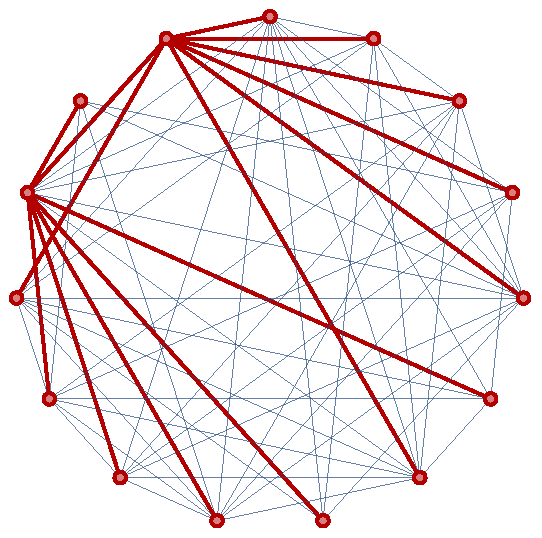
\includegraphics[width=0.8\columnwidth]{mst}
\caption{A random graph (blue) with an MST highlighted (red).} \label{fig:mst}
\end{figure}

The calculation of MSTs is most likely to come into consideration when actually performing the initial construction of networks, where we wish to connect all nodes in the network, but using the most frugal possible physical resources. MSTs serve this purpose, and since they are trees, inherit all the same properties of tree networks.

%
% Random
%

\subsection{Random} \index{Random topologies}

A variation on the complete graph, $K_{|V|}$, is to instead have a randomised implementation of it, whereby each of the possible edges in $K_{|V|}$ occurs with probability \mbox{$0\leq p_\text{edge}\leq 1$}. We would thereby be able to tune between the complete graph and the completely disconnected graph, representing a randomly connected network with arbitrary average connectivity. Specifically, the average number of links emanating from any node is \mbox{$e_\text{av} = (|V|-1)p_\text{edge}$}. Note that random graphs might be disjoint, making them inappropriate for many networking applications. For asymptotically large random graphs, \textit{percolation theory} \cite{???} provides thresholds for $p_\text{edge}$ such that they remain connected \cite{???}. Fig.~\ref{fig:random_graph} illustrates several graphs with different edge connectivity probabilities.

\begin{figure}[!htb]
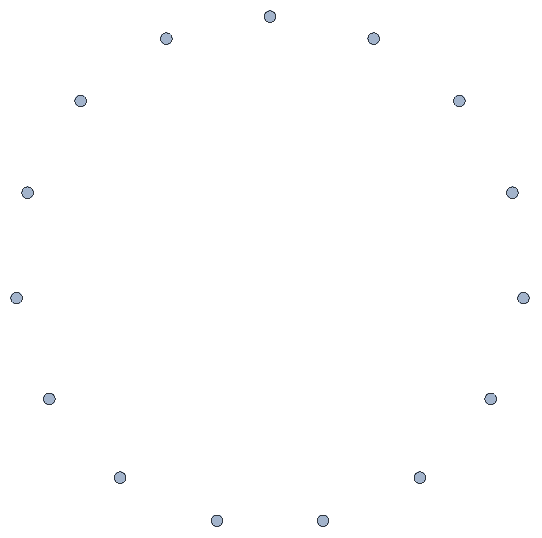
\includegraphics[width=0.6\columnwidth]{random_0}
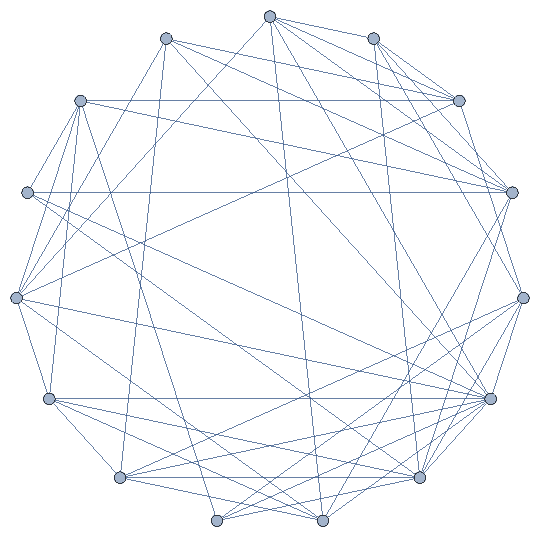
\includegraphics[width=0.6\columnwidth]{random_05}
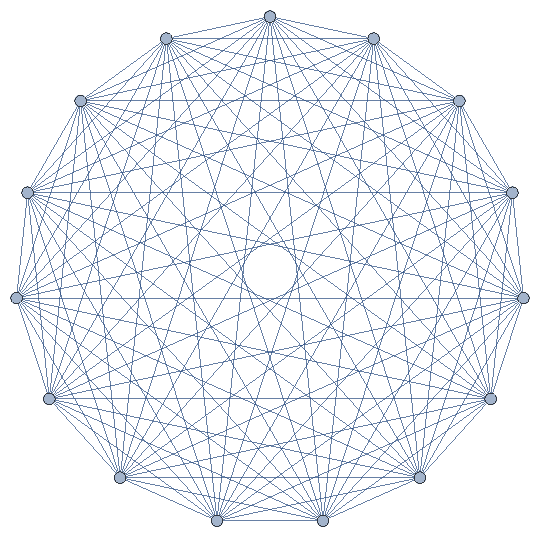
\includegraphics[width=0.6\columnwidth]{random_1}
\caption{The 15-vertex randomly-connected graph. This is the same as $K_{15}$ in Fig.~\ref{fig:complete_graph}, but where edges are present with probabilities \mbox{$p_\text{edge}=0,0.5,1$} (top to bottom).} \label{fig:random_graph}
\end{figure}

Random graphs capture the ad hoc nature of networks that exhibit no planned structure, but are rather cobbled together in a completely improvised manner.

%
% Hybrid
%

\subsection{Hybrid} \index{Hybrid topologies}

Real networks are highly unlikely to fit the exact form factor of any of the classes of graphs presented above. Rather, a truly global internet is inevitably going to comprise many subnetworks, each structured completely independently of one another, with little consistency or large-scale planning between them. Who thinks about the broader structure of the global internet when setting up their office network?

For example, at the global scale, it is entirely plausible that the internet might take on a random tree-like structure. But when we get down to a lower level, the tree structure vanishes and is replaced by all manner of different network topologies, run and maintained by different organisations in their own distinct ways.

Furthermore, the real-world internet is not simply a hierarchy of different types of well-known graph structures. Rather, it takes the form of `glued' graphs, whereby networks running over different mediums, or via different operators, each exhibit their own independent graph topologies, meeting at interconnect points that join the different networks. Typically this yields redundancy in the routes between different nodes, ushering in the need for combinatorial optimisation techniques when allocating network resources.

This hybrid network topology is the norm today in our classical internet, and it is entirely foreseeable that a similar trend will emerge in the future quantum internet as quantum technologies become more mainstream, their networking less well structured, and competing, redundant links are in place.

%
% The Internet Webgraph
%

\subsection{The internet webgraph} \index{Internet webgraph}

Of course, all the topological structures described until now are in-principle constructs. Of most relevance is the \textit{Webgraph}, the graph of the actual internet (or some other real-world network). Fig.~\ref{fig:webgraph} illustrates some example webgraphs. The combination of random, densely and sparsely connected, and tree structures, and its clear hierarchy are all evident. This encourages our intuition of the different types of structures present in realistic networks.

\begin{figure}[!htb]
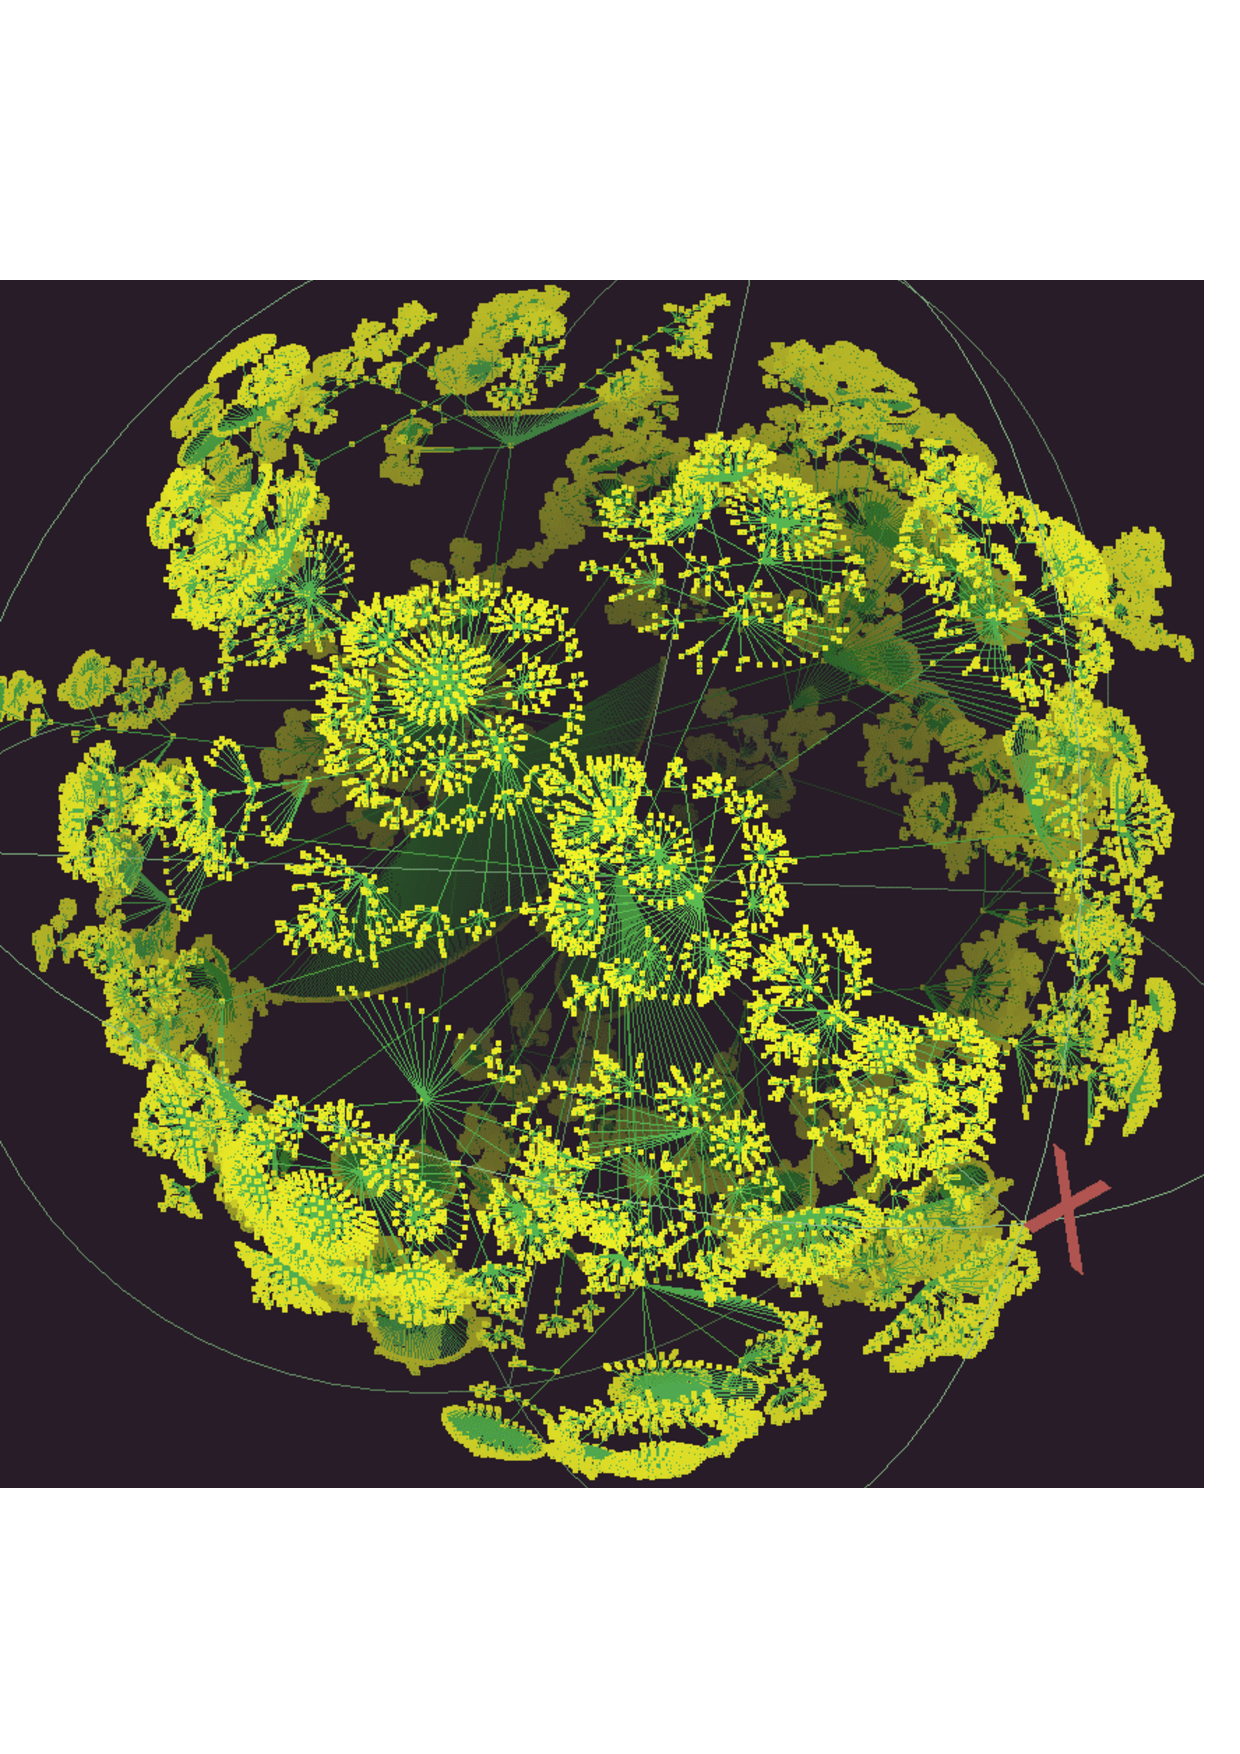
\includegraphics[width=\columnwidth]{webgraph_1} \\
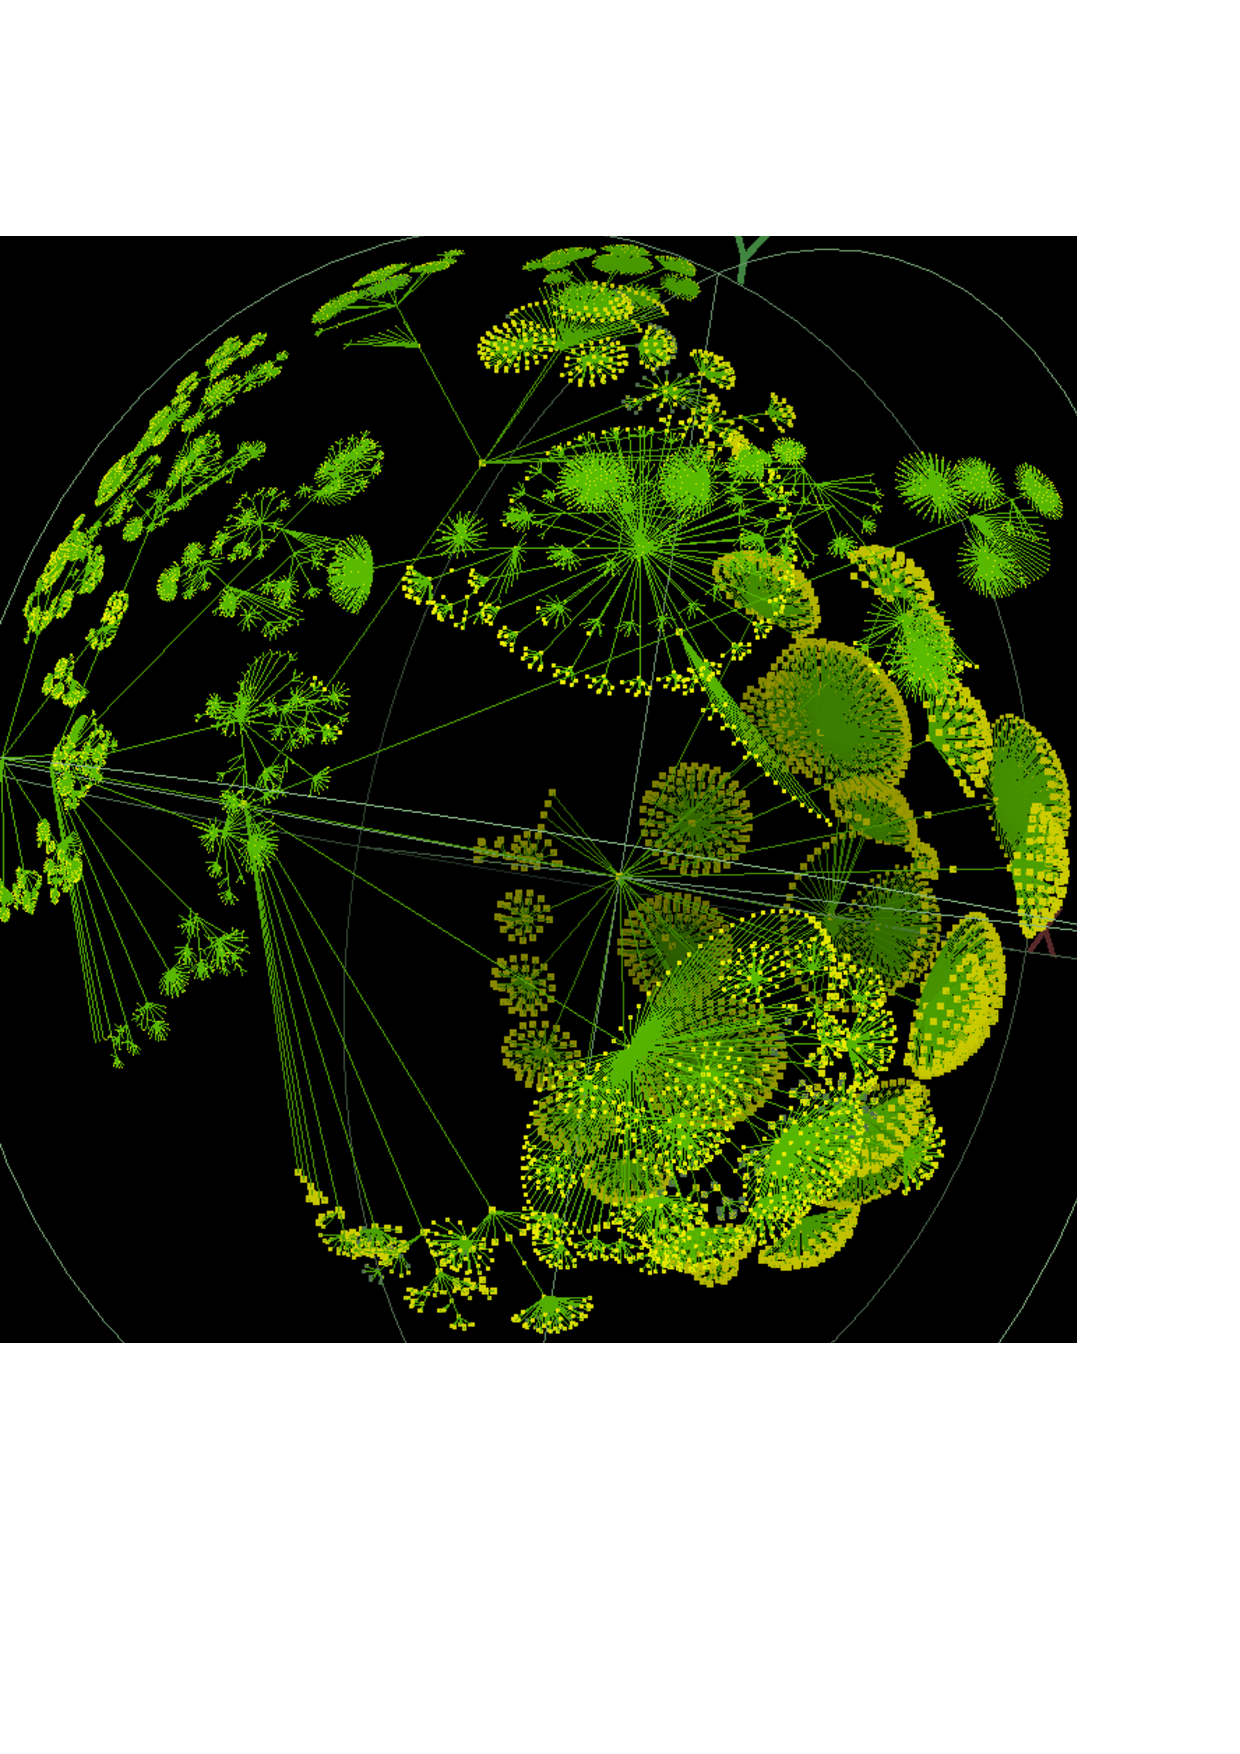
\includegraphics[width=\columnwidth]{webgraph_2}
\caption{Examples of real-world webgraphs, capturing their high-level random tree-like structure. Graphics attributed to the Center for Applied Internet Data Analysis (CAIDA), \texttt{\href{http://www.caida.org}{http://www.caida.org}}.} \label{fig:webgraph}
\end{figure}

%
% Scale-Free Networks
%

\subsection{Scale-free networks}

\comment{To do}

%
% Network Algorithms
%

\section{Network algorithms} \label{sec:graph_theory} \index{Network algorithms}

Having introduced some of the more relevant graph structures, we now introduce some of the key graph-theoretic algorithms of direct relevance to networking theory \cite{bib:RivestAlgBook}. In graph theory, many fundamental problems are believed to be computationally hard to solve, often \textbf{NP}-complete\index{\textbf{NP} \& \textbf{NP}-complete}. However, there are several important graph algorithms that are (very) classically efficient to solve, and which are of great utility to us as network architects.

We will focus heavily on combinatorial optimisation techniques, where the goal is to allocate network resources so as to optimise some cost metric. This includes both single- and multi-user algorithms, the latter being the far more relevant ones in the context of shared networks like the internet.

In Table.~\ref{tab:net_alg_sum} we summarise the upcoming discussion on important network algorithms, and their associated complexities.

\renewcommand{\tablename}{TABLE}

\begin{table*}[!htb]
	\begin{tabular}{|c|c|c|c|}
		\hline
  		Algorithm & Description & Complexity class & Scaling \\
  		\hline
  		\hline
  		Breadth-first-search & Explore all vertices in a graph & \textbf{P} & $O(|V|+|E|)$ \\
  		\hline
  		Depth-first-search & (same as above) & \textbf{P} & $O(|V|+|E|)$ \\
		\hline
  		Shortest-path (Dijkstra) & Find the shortest route between two nodes & \textbf{P} & $O(|V|^2)$ \\
  		& in a directed graph & &  \\
  		  		\hline
		Shortest-path (\textit{A*}) & (same as above) & \textbf{P} & (varying) \\
  		  		\hline
		Single-source shortest path & Find the shortest paths from a given node to & \textbf{P} & $O(|V|\cdot |E|)$\\
  		& \emph{all} other nodes & & \\
 		\hline
Minimum spanning tree & Find a spanning tree of a graph that minimises & \textbf{P} & $O(|E|\text{log}|V|)$ \\
  		& the total of the edge weights & & \\
  		\hline
  		Minimum cost flow & Minimise total costs in a network &  \textbf{P} & $O(|V|\text{log}|V|(|E|$\\
  		(Orlin)& with a specified amount of flow& & $+|V|\text{log}|V|))$ \\
  		\hline
  		Maximum flow & Maximise flow in a network, regardless of costs & \textbf{P} & $O(|E|\cdot c_\text{max})$ \\
  		(Ford-Fulkerson) & & & \\
  		\hline
  		Multi-commodity flow & Same as maximum flow, but generalised to & \textbf{NP}-complete & ? \\
  		& arbitrary numbers of users & (exactly), & \\
  		& & \textbf{P} (approximation & \\
  		& & using heuristics) & \\
  		\hline
  		Vehicle routing problem & Generalises the shortest-path algorithm to multiple & \textbf{NP}-complete & ? \\
  		& users, with distinct sources and destinations & & \\ 
  		\hline
  		Vehicle rescheduling problem & Same as above but with dynamically changing costs & \textbf{NP}-complete & ? \\
    	\hline
	\end{tabular}
	\caption{Summary of some important network algorithms and their complexities. The \textbf{NP}-complete algorithms are not believed to have efficient classical algorithms, and their exact scaling is not well understood.} \label{tab:net_alg_sum} \index{Network algorithms}
\end{table*}

\renewcommand{\tablename}{ALG.}

%
% Network Exploration & Pathfinding
%

\subsection{Network exploration \& pathfinding} \label{sec:path_exp} \index{Network exploration \& pathfinding}

Here the goal is to systematically explore every vertex in an unknown graph exactly once, so as to reconstruct the entire network graph, or to find a target node with unknown location (which can obviously be achieved if the former can be). The two main approaches are \textit{breadth-first-search} (BFS) and \textit{depth-first-search} (DFS) algorithms\index{Breadth-first-search (BFS) algorithm} \index{Depth-first-search (DFS) algorithm}. In both cases we begin at a starting (root) node, from which we wish to explore the entire graph by only following edges to nearest neighbours one at a time.

In BFS we proceed from the root node to visit every one of its neighbours. Having done so, and created a list of those neighbours, we proceed onto the neighbours of the neighbours, and so on, until every vertex in the graph has been visited, or the target node found.

In DFS, on the other hand, we begin by following a single arbitrary path until we reach a dead-end, at which point we backtrack until we reach a branch leading to a vertex we hadn't previously visited.

Examples of these two algorithms are shown in Fig.~\ref{fig:BFS_DFS}.

\begin{figure}[!htb]
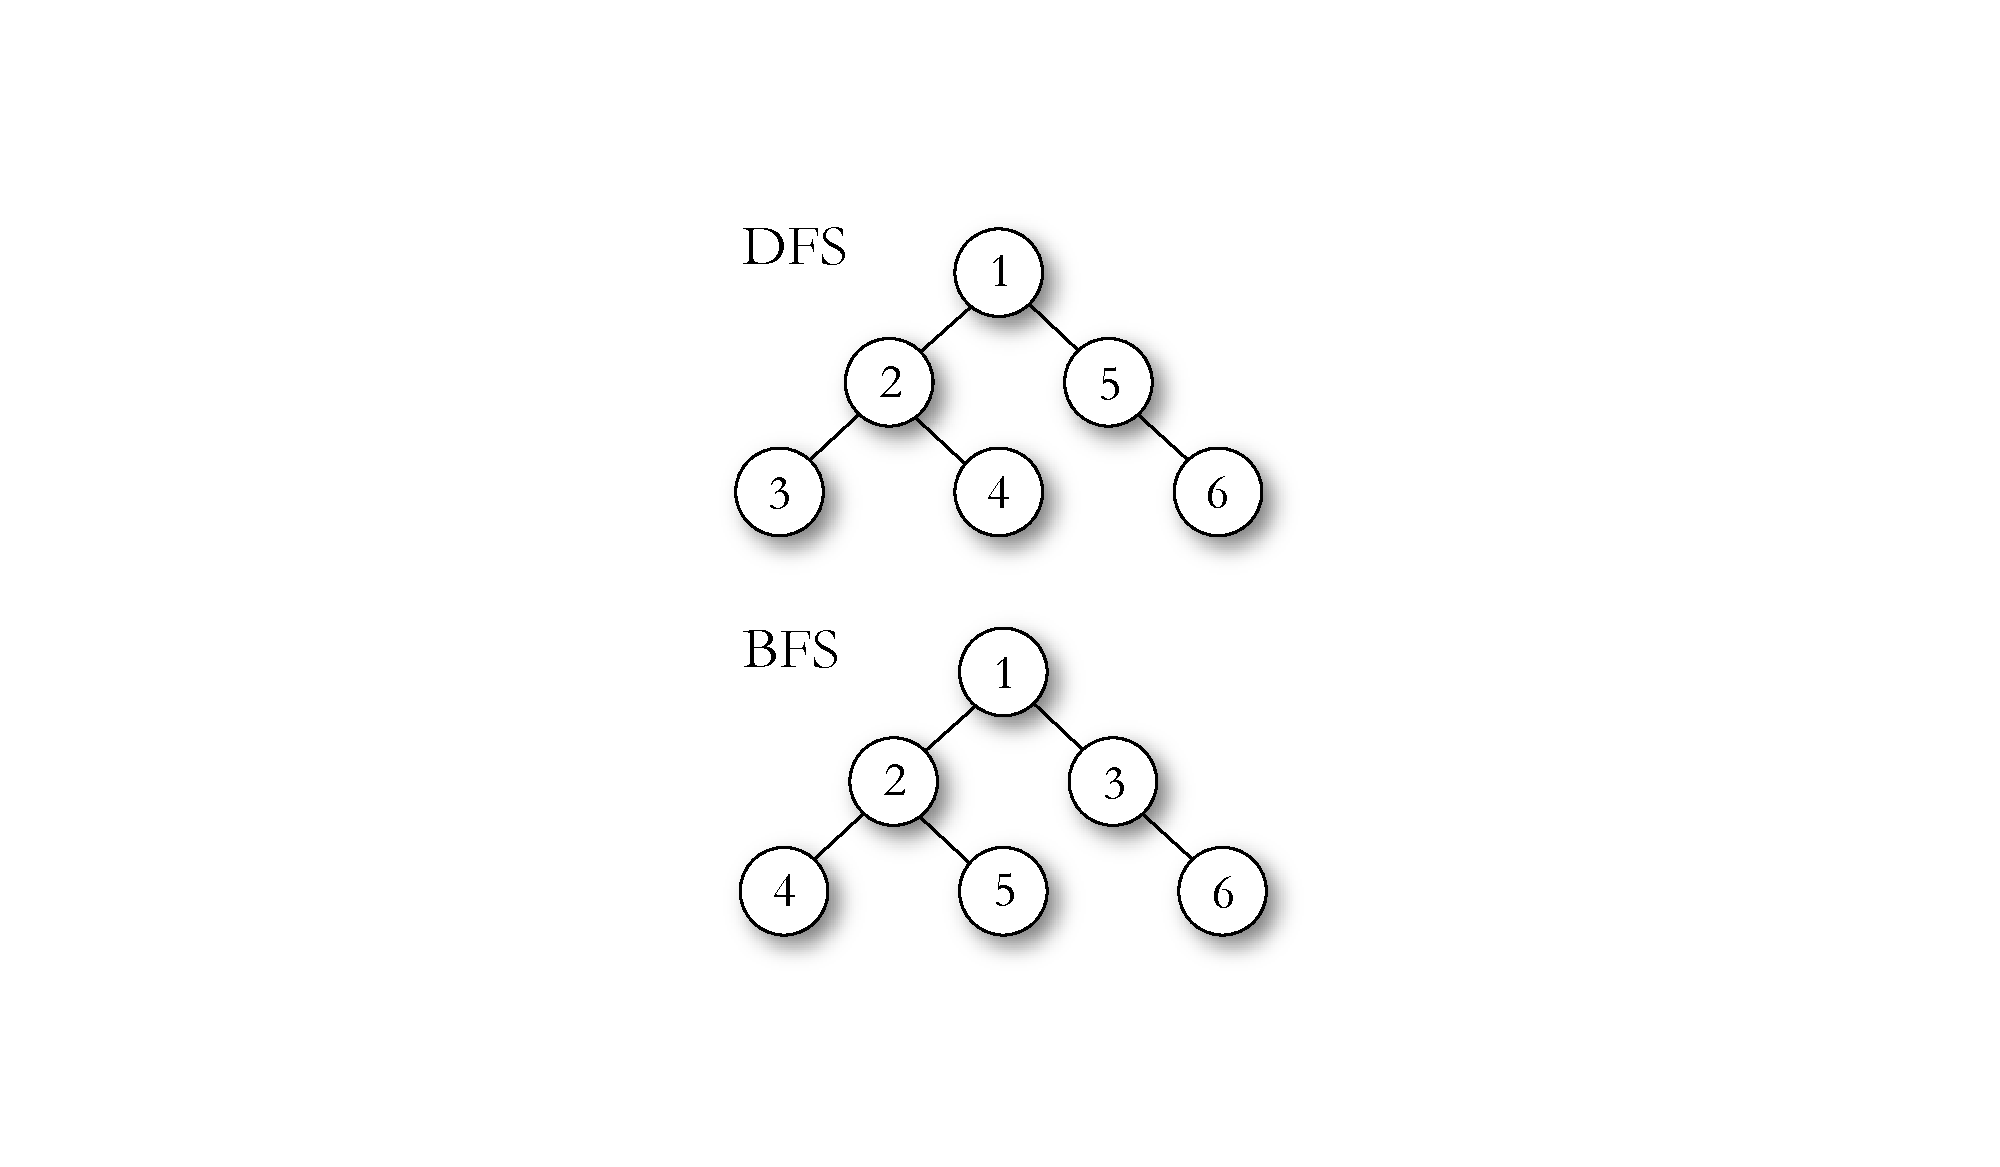
\includegraphics[width=0.6\columnwidth]{BFS_DFS}
\caption{Comparison of the order in which vertices are explored, using the breadth-first-search (BFS) and depth-first-search (DFS) algorithms, where vertex 1 is the root vertex.} \label{fig:BFS_DFS}
\end{figure}

Both BFS and DFS guarantee visiting every vertex in a connected graph, and do so using only nearest neighbour transitions. Such algorithms are therefore very useful for network discovery.

The BFS algorithm is particularly applicable to pathfinding in ad hoc networks. Consider the situation where there is no central authority with full knowledge of the network, overseeing network operation. Rather, everyone needs to figure things out for themselves by only interrogating their neighbours, to whom they have direct connections. This directly leads to a BFS algorithm, where a node speaks to each of its neighbours in turn, who subsequently do the same thing, yielding a recursive algorithm. This can be naturally parallelised, as each node can be interrogating its neighbours independently, thereby implementing a distributed BFS algorithm. Note that, when searching for a target node, while the BFS algorithm obviously finds the target using the smallest number of hops (i.e a lowest-order route), it needn't necessarily find the route with the lowest cost (which is distinct from the number of hops in general). Shortest-path algorithms require a priori knowledge of the full network graph, discussed in Sec.~\ref{sec:shortest_path}.

Both BFS and DFS exhibit runtime \mbox{$O(|V|+|E|)$}, where $|V|$ and $|E|$ are the number of vertices and edges respectively. Thus, these graph exploration algorithms reside in the complexity class \textbf{P}, and are classically efficient.

%
% Shortest-Path
%

\subsection{Shortest-path} \label{sec:shortest_path} \index{Shortest-path algorithm}

In graph theory, the shortest-path problem is that of finding a subgraph of a given graph $G$, connecting two vertices, \mbox{$A\to B \subset G$}, such that the sum of its edge weights is minimised. In the context of our application to route-finding, this amounts to finding a route that minimises cost.

The first proven shortest-path algorithm was by Dijkstra \cite{bib:Dijkstra59}, which requires runtime $O(|V|^2)$, also residing in \textbf{P}\index{\textbf{P} \& \textbf{BPP}}. Subsequently, a number of improvements and variations on Dijkstra's algorithm have been proposed, most notably the $A^*$ algorithm \cite{bib:Astar}, which has found widespread modern use, using a heuristic approach to improve performance over Dijkstra.

Formally, let $\vec{R}$ be the set of all routes \mbox{$A\to B$}. Then,
\begin{align}
c_\text{opt} = \min_{r\in R} \left(\sum_{i\in r} c_\text{net}(i) \right),
\end{align}
where \mbox{$i\in r$} denotes the $i$th edge in the route $r$. Intuitively, the (in general) exponential number of possible paths through a graph might lead one to believe the above optimisation problem is a computationally inefficient one (such as \textbf{NP}-complete, or worse). However, perhaps surprisingly, Dijkstra's algorithm cleverly manages to reduce this to a polynomial-time problem. A sketch of the algorithm is provided in Alg.~\ref{alg:dijkstra}, which needn't be understood by the reader desperate to read further.

\begin{table}[!htb]
\fbox{\parbox{0.965\columnwidth}{\texttt{ 
function DijkstraShortestPath($G$,$A$,$B$):
\begin{enumerate}
	\item currentNode = $A$
    \item tentativeDistances[$A$] = 0
    \item tentativeDistances[others] = $\infty$
    \item nodesVisited[$A$] = True
    \item nodesVisited[others] = False
    \item loopStart:
    \item neighbours = currentNode.neighbourhood
    \item nodesVisited[neighbours] = True
    \item for(n$\in$neighbours) \{
    \setlength{\itemindent}{0.2in}
    \item newTentativeDist = \\ min(tentativeDistances[currentNode] \\+ edgeWeight[currentNode,n],\\
        tentativeDistances[n])\\
    \item nodesVisited[currentNode] = True
    \setlength{\itemindent}{0in}
    \item \}
    \item if(nodesVisited[$B$] = True) \{
    \setlength{\itemindent}{0.2in}
	\item return(tentativeDistances[$B$])
	\item $\Box$
    \setlength{\itemindent}{0in}
    \item \}
	\item currentNode = \\
	tentativeDistances[unvisitedNodes].\\
	nodeWithSmallest()
	\item goto(loop)
    \item $\Box$
\end{enumerate}}}}
\caption{Dijkstra's original shortest-path algorithm for finding the lowest weight path through a graph, $G$, between two vertices, $A$ (source) and $B$ (destination). The algorithm has $O(|V|^2)$ runtime (in \textbf{P}). \comment{Fix me}} \label{alg:dijkstra}\index{Shortest-path algorithm}
\end{table}

Fig.~\ref{fig:simp_route_opt} illustrates a directed, edge-weighted graph. A shortest-path algorithm applied between vertices $A$ and $B$ would return \mbox{$R_\text{shortest} = A\to F\to B$} as the minimum cost route.

When introducing network graphs earlier, we insisted upon all costs being associated with edges rather than vertices, and presented a trivial means by which to convert vertex costs to edge costs in Fig.~\ref{fig:remove_nodes}. This adamance arose because the presently described shortest-path algorithms operate purely in terms of edge weights, not vertex weights. But the mapping we presented from the latter to the former obviates this issue.

This is the motivating factor behind representing network graphs purely in terms of edge weights (Sec.~\ref{sec:quant_proc_in}), thereby enabling compatibility with shortest-path algorithms.

For the purposes of the QTCP protocol, we are interested in the case of directed graphs (recall that in terms of cost metrics, undirected graphs can be converted to directed graphs by replacing undirected edges with a pair of identical edges in opposite directions).

Shortest-path techniques find widespread application in many areas. Computer networks are an obvious candidate, since networks are inherently graph-theoretic by nature.

To implement the shortest-path algorithms discussed above, the party performing the calculation requires knowledge of the full network graph. In an ad hoc network, where users might be added to or removed from the network arbitrarily, this isn't necessarily the case.

One solution is for a central authority to be responsible for maintaining a ledger of all network participants and their connectivity, which users are required to notify upon joining or leaving the network. The central authority may then apply shortest-path calculations, which may be queried by users. However, a disruption in connection to the central authority, or failure of nodes to notify the central authority upon joining or leaving the network, introduces a point of failure into the operation of the protocol.

Another approach, which does not require a reliable central authority, is for users to implement network exploration algorithms each time they wish to perform a shortest-path calculation. This facilitates truly ad hoc networking, but incurs the cost overhead associated with nodes frequently implementing network exploration. However, network exploration is a purely classical algorithm, which may run entirely over the classical network, and therefore incurs no cost in quantum resources.

With this approach, a new node can join the network, without having to know anything about the topology of the network. Similarly, upon leaving the network, it needn't notify anyone, since a future interrogation by a neighbour will be detected as a non-existent node. The BFS is therefore highly suited to ad hoc operation. In fact, present-day internet gateway protocols (Sec.~\ref{sec:gateway}) essentially implement a distributed version of BFS.

%
% Single-Source Shortest-Path Algorithm
%

\subsection{Single-source shortest-path} \label{sec:single_source_sp} \index{Single-source shortest path algorithm}

The shortest-path algorithm by Dijkstra presented above finds the shortest route between two specified nodes in a network. However, when employing \textsc{Individual} routing strategies, where there is no central mediation of the network, each node desires an up-to-date routing table, showing the best route to take to any other point in the network. Then, upon receiving packets with particular destinations, rather than repeatedly applying Dijkstra's algorithm, we can simply look up the destination on the node's local routing table.

Single-source shortest-path algorithms address this problem by calculating the shortest paths from the current node to \textit{every} other node in the network topology.

The best-known algorithm for this problem is the Bellman-Ford (or Bellman-Ford-Moore)\index{Bellman-Ford-Moore algorithm} algorithm \cite{BF}, which requires worst-case runtime of $O(|V|\cdot |E|)$. Clearly this is more complex than Dijkstra's algorithm for finding a particular shortest-path. But it is more efficient than using brute-force to find the shortest-path between every pair of nodes in the network via $O(|V|^2)$ repeated applications of Dijkstra.

%
% Minimum Spanning Tree
%

\subsection{Minimum spanning tree} \label{sec:min_tree} \index{Minimum spanning tree algorithm}

MST algorithms find an MST\footnote{There may be multiple distinct MSTs for a given graph.} of some arbitrary graph. Like the shortest-path problem, it has a polynomial-time, deterministic algorithm (i.e it resides in \textbf{P}\index{\textbf{P} \& \textbf{BPP}}). The first MST algorithm \cite{bib:Boruvka26} required $O(|E|\log |V|)$ runtime. Numerous variations have since been proposed, with little change to the underlying scaling.

Because MST algorithms are efficient, they play a very useful role in the design of real-world network topologies, where resource minimisation is crucial.

Fig.~\ref{fig:mst} shows an example of a graph with its MST.

%
% Minimum Cost Flow
%

\subsection{Minimum cost flow} \label{sec:min_cost_flow_prob} \index{Minimum cost flow algorithm}

The \textit{minimum cost flow problem} \cite{???} is that of minimising costs through a network for a specified amount of flow (i.e total bandwidth or throughput), which acts as a constraint on the problem. The definition of `cost' in this context is compatible with our earlier definition of cost metrics (Def.~\ref{def:metric}).

This problem can be efficiently solved using linear programming. Specifically, cost metrics along links in series are given by linear combinations of individual link costs. If, in addition, we let our net cost function be linear in the constituent costs then the net cost will also be linear in all the edge weights. This lends itself directly to optimisation via linear programming techniques. Algorithms for linear programming, such as the \textit{simplex} algorithm, have polynomial-time solutions (i.e reside in \textbf{P}\index{\textbf{P} \& \textbf{BPP}}), and a plethora of software libraries are available for implementing them numerically.

One polynomial-time algorithm for solving this problem does so in \mbox{$O(|V|\text{log}|V|(|E|+|V|\text{log}|V|))$} time \cite{JAMES_B_ORLIN}.

%
% Maximum Flow
%

\subsection{Maximum flow} \label{sec:max_flow_prob} \index{Maximum flow algorithm}

The \textit{maximum flow problem} \cite{???} is the seemingly simple goal of -- as the name suggests -- maximising network flow, without consideration for any of the other cost metrics or attributes associated with the network. This type of problem is relevant when brute bandwidth is the dominant goal.

This problem can be tackled using a number of techniques. In some circumstances, linear programming techniques can be employed. The best-known algorithm is the Ford-Fulkerson algorithm \cite{???}, which finds a solution in \mbox{$O(|E|\cdot c_\text{max})$} runtime, where $|E|$ is the number of links in the network and $c_\text{max}$ is the maximum cost present in the network. The algorithm behaves pathologically in some conditions, which can easily be overcome in the context we present here. Using Ford-Fulkerson as a starting point, numerous other more sophisticated algorithms have been developed.

%
% Multi-Commodity Flow
%

\subsection{Multi-commodity flow} \label{sec:multi_comm_flow} \index{Multi-commodity flow algorithm}

The \textit{multi-commodity flow problem} \cite{???} generalises the previous algorithms to be applicable to multi-user networks. The generalisation is that there may be a number of distinct senders, residing on different nodes, each transmitting to distinct recipients, residing on different nodes. This is the most realistic scenario we are likely to encounter in a real-world quantum internet, where networks will inevitably be shared by many users, residing at different nodes.

Unfortunately the computational complexity of solving this problem is much harder than the previous algorithms in general. Specifically, solving the problem exactly is \textbf{NP}-complete\index{\textbf{NP} \& \textbf{NP}-complete} in general. However, in specific circumstances it can be approached using linear programming or polynomial-time approximation schemes.

%
% Vehicle Routing Problem
%

\subsection{Vehicle routing problem} \label{sec:VRP} \index{Vehicle routing problem}

The vehicle routing problem (VRP) is a multi-user generalisation of the shortest-path problem, where the goal is to minimise total network cost (i.e the sum of all individual users' costs) when there are multiple users sharing the network, each with distinct sources and destinations.

Unlike the polynomial-time shortest-path algorithm, exactly solving the VRP is \textbf{NP}-hard\index{\textbf{NP} \& \textbf{NP}-complete} in general. However, heuristic methods can find approximate suboptimal solutions far more efficiently, and there is a multitude of software packages available for doing so.

The VRP has found widespread use in, for example, the routing of transport networks for delivery companies or public transportation networks (hence the name), and many commercial companies exist, which perform these kinds of optimisations on behalf of transport providers to enhance their efficiency.

It is obvious that this algorithm is directly applicable to multi-user communications networks, which are conceptually identical to transport networks, albeit a bit faster. 

A multitude of variations on the VRP exist, accommodating for different types of constraints (or additional flexibilities) in the operation of the network.

%
% Vehicle Rescheduling Problem
%

\subsection{Vehicle rescheduling problem} \label{sec:VRSP} \index{Vehicle rescheduling problem}

The vehicle rescheduling problem (VRSP) generalises the VRP to the case where properties of the network undergo changes dynamically within the course of transmissions over the network. To use the analogy of transport networks, this could entail, for example, a truck breaking down en route to its destination, requiring real-time rescheduling of the other vehicles.

Solving the VRSP exactly is \textbf{NP}-complete\index{\textbf{NP} \& \textbf{NP}-complete} in general, but as with the VRP, heuristic methods can often be applied, which efficiently find approximate solutions.

In the context of communications over networks, the VRSP has obvious applicability -- a quantum internet is likely going to be largely ad hoc in nature, with users coming and going, and many non-deterministic points of failure, requiring ongoing updating of routing decisions if resource allocation is to remain as efficient as possible.

%
% Improving Network Algorithms Using Quantum Computers
%

\subsection{Improving network algorithms using quantum computers} \index{Network algorithms on quantum computers}

Given that we are directing this work at the upcoming quantum era, where quantum computing will become a reality, it is pertinent to ask whether quantum computers might improve the aforementioned network algorithms, some of which are computationally hard problems. Most notably, several of the discussed algorithms are \textbf{NP}-complete\index{\textbf{NP} \& \textbf{NP}-complete} in general, a complexity class strongly believed to be exponentially complex on classical computers. Can quantum computers help us out here, and improve network resource allocation?

While it is not believed that quantum computers can efficiently solve such \textbf{NP}-complete\index{\textbf{NP} \& \textbf{NP}-complete} problems, it is known that they can offer a quadratic speedup using Grover's unstructured search algorithm. Specifically, \textbf{NP}-complete\index{\textbf{NP} \& \textbf{NP}-complete} problems can be treated as satisfiability problems, where we are searching for an input to a classical algorithm that yields a particular output.

To gain a quantum advantage, we treat the classical algorithm as an oracle whose input configurations form an unstructured search space. Then, Grover's algorithm can perform a search over the space of input configurations to find a satisfying solution, with quadratically enhanced runtime.

While a quadratic improvement is far short of the exponential improvement we might hope for, Grover's algorithm is known to be optimal for the unstructured search problem \cite{?}. Nonetheless, despite only yielding a quadratic improvement, a quadratic speedup may already be sufficient to significantly improve network resource allocation.

%
% Optical Routers
%

\section{Optical routers} \index{Optical routers}

Perhaps the most fundamental building block in any network is routers, devices which switch data packets between multiple inputs and outputs so as to relay them to a destination. Indeed, in many real-world networks, many nodes will purely implement routing, and nothing more elaborate such as computations or other end-user protocols, to be discussed in Sec.~\ref{sec:protocols_quant_int}.

We now discuss the implementation of optical routers, beginning with the simplest two-port switch, upon which we build to construct more general and powerful routers.

We will use the terminology that:
\begin{itemize}
	\item \textit{Ports}\index{Ports}: refers to the number of input and output optical modes in a device.
	\item \textit{Channels}\index{Channels}: refers to the number of simultaneous communications streams running in parallel through the device.
	\item \textit{Optical depth}\index{Optical depth}: is the number of primitive optical elements/devices a light path traverses through the course of its trajectory from input to output.
\end{itemize}

A summary of the routing devices we consider, and their associated resource requirements, is provided in Table.~\ref{tab:router_summary}.

Of course, real-world routers will not only switch optical paths, but also implement some (probably undesired) quantum processes across those paths, such as a loss channel or temporal mode-mismatch. Thus, proper analysis of optical router performance in quantum networks requires treating them as legitimate nodes in the network graph, with associated costs and attributes, as per the QTCP framework.

\renewcommand{\tablename}{TABLE}

\begin{table*}[!htb]
	\begin{tabular}{|c|c|c|}
		\hline
  		Device & Resource requirements & Optical depth \\
  		\hline
  		\hline
  		Two-channel two-port switch & \mbox{$N_\mathrm{bs}=2$}, \mbox{$N_\mathrm{ps}=1$} & \mbox{$d=1$} \\
  		Linear $n$-port multiplexer & \mbox{$N_\mathrm{s}=n-1$} & \mbox{$1\leq d\leq n-1$} \\
  		Pyramid $n$-port multiplexer & \mbox{$N_\mathrm{s}=n-1$} & \mbox{$d=\mathrm{log}_2(n)$} \\
    	Single-channel multi-port switch (linear) & \mbox{$N_\mathrm{s}=2n-3$} & \mbox{$2\leq d\leq 2n-3$} \\
  		Single-channel multi-port switch (pyramid) & \mbox{$N_\mathrm{s}=2n-3$} & \mbox{$d=2\,\mathrm{log}_2(n)-1$} \\
  		Multi-channel multi-port switch & \mbox{$N_\mathrm{s} = \left\lceil \frac{n^2}{2}\right\rceil - n + 1$} & \mbox{$\left\lceil \frac{n}{2} \right\rceil \leq d\leq n-1$} \\
    	\hline
	\end{tabular}
	\caption{Summary of different primitives for constructing optical routers. $n$, $N_\mathrm{bs}$, $N_\mathrm{ps}$ and $N_\mathrm{s}$ are the number of input/output ports, beamsplitters, phase-shifters, and two-port switches respectively. $d$ is the optical depth (in units of number of two-port switches). Since all of the multi-port devices are constructed from two-port switches, in all cases \mbox{$N_\mathrm{bs} = 2 N_\mathrm{s}$} and \mbox{$N_\mathrm{ps} = N_\mathrm{s}$}.} \label{tab:router_summary} \index{Optical routers}\index{Optical depth}\index{Router resource requirements}
\end{table*}

\renewcommand{\tablename}{ALG.}

%
% Interferometric Routers
%

\subsection{Interferometric routers} \index{Interferometric routers}

Interferometric routers are based on the principle that the evolution implemented by an interferometer is in general highly dependent on the phase relationships within it. This reduces the seemingly uphill task of high-speed, dynamic switching between modes to the problem of implementing dynamically-controllable phases. Thankfully there are a number of techniques for implementing such phase-switching. We will discuss these phase-modulation techniques, before moving onto combining them into more complex routing systems.

%
% Phase-Modulators
%

\subsubsection{Phase-modulators} \index{Phase-modulators}

A phase-modulator is a classically-controlled device that lets us tune the local phase accumulated by an optical path, ideally over the full range of $\{0,2\pi\}$. These may be implemented in several ways:

%
% Electro-Optic Modulators
%

\paragraph{Electro-optic modulators (EOMs)} \index{Electro-optic modulators}

\comment{here an applied electric field induces a change in refractive index in a medium, causing a phase-shift.}

\comment{To do! Explain how these work}

%
% Acousto-Optic Modulators
%

\paragraph{Acousto-optic modulators (AOMs)} \index{Acousto-optic modulators}

\comment{an applied acoustic wave generated by a piezoelectric transducer induces a change in refractive index in a medium, causing a phase-shift}

\comment{To do! Explain how these work}

%
% Magneto-Optic Modulators
%

\paragraph{Magneto-optic modulators} \index{Magneto-optic modulators}

\comment{an applied magnetic field induces the change in refractive index}

\comment{To do! Explain how these work}

%
% Pockels Cells
%

\paragraph{Pockels cells} \index{Pockels cells}

\comment{act as voltage-controlled wave-plates, 	which take the place of phase-shifters in a polarisation-encoded version of Mach-Zehnder interference.}

\comment{To do! Explain how these work}

%
% Two-Channel Two-Port Switches
%

\subsubsection{Two-channel two-port switches} \index{Two-channel two-port switches}

The elementary primitive switch from which more complicated routers may be constructed is the two-channel two-port switch. This switch may be constructed from a Mach-Zehnder interferometer\index{Mach-Zehnder (MZ) interference}, with a classically-controlled phase-shifter in one arm. By switching the phase to either \mbox{$\phi=0$} or \mbox{$\phi=\pi$}, the MZ may be tuned to implement either an identity or swap operation respectively. This is shown in Fig.~\ref{fig:two_channel_two_port_switch}.

In the upcoming diagrams we present, arrows are used to indicate the time-ordering of the flow of data. However, it should be noted that a MZ interferometer is reversible and therefore bidirectional, and so too are all of the more complex routers based upon them.

\begin{figure}[!htb]
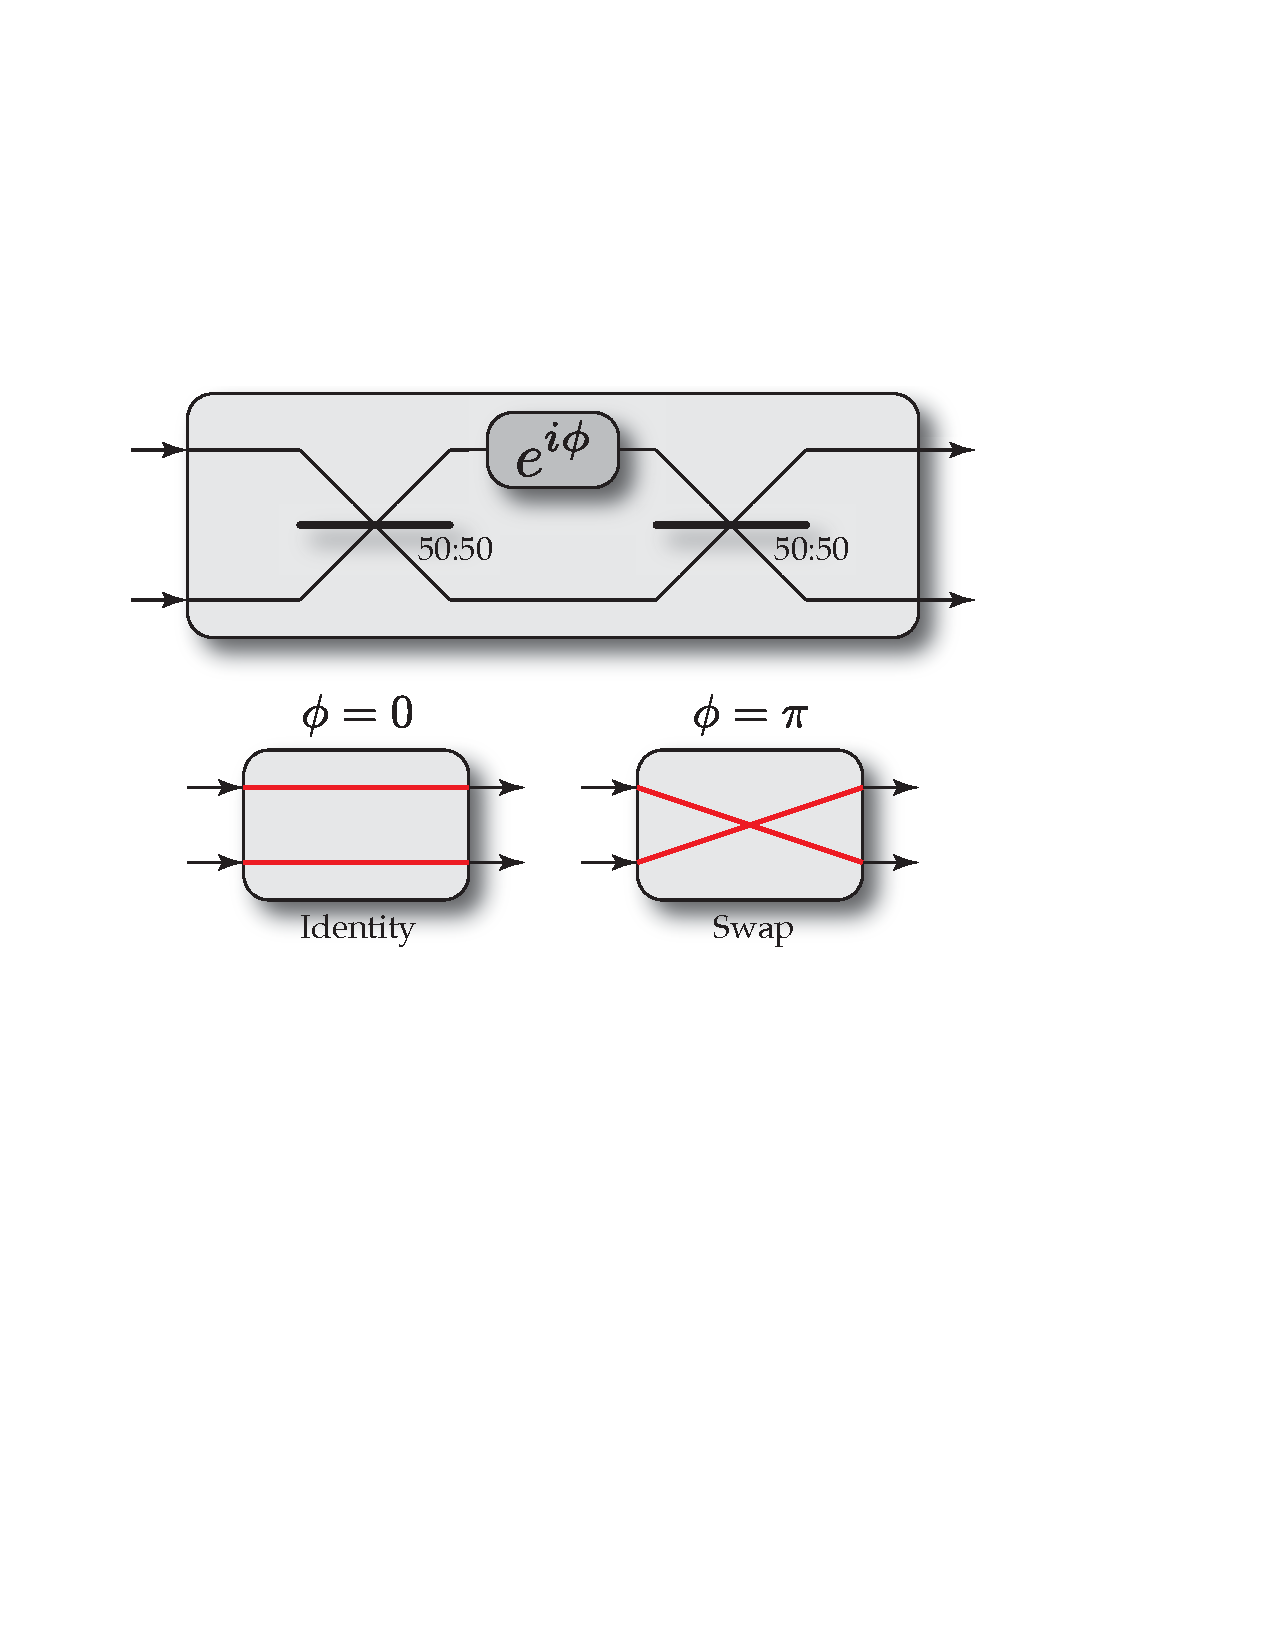
\includegraphics[width=\columnwidth]{two_channel_two_port_switch}
\caption{(top) A two-channel two-port switch has two inputs and two outputs, implementing either an identity or swap operation between them. This may be constructed using a Mach-Zehnder interferometer with a variable, classically-controlled phase-shift, $e^{i\phi}$, in one of the arms, which may be implemented using an acousto-optic or electro-optic modulator (AOM or EOM). The phase-shift is allowed to be either \mbox{$\phi=0$} for an identity channel (bottom left) or \mbox{$\phi=\pi$} for a swap operation (bottom right). Because the switch is based on MZ interference, this technique only applies to optical states which undergo MZ interference. The total resource requirements are two 50:50 beamsplitters and a single phase-shifter.} \label{fig:two_channel_two_port_switch} \index{Two-channel two-port switches}\index{Mach-Zehnder (MZ) interference}
\end{figure}

Because the two-port switch is based upon MZ interference, it will only function for optical states subject to such MZ interference. Thus, single-photons and coherent states are applicable, whereas thermal states, for example, are not.

%
% Multiplexers & Demultiplexers
%

\subsubsection{Multiplexers \& demultiplexers} \index{Multiplexers}\index{Demultiplexers}

From the two-port switch, which implements a controlled permutation of two optical modes, we can construct multi-port multiplexers and demultiplexers, which controllably route a single input port to one of $n$ multiple output ports, or vice versa.

There are two main architectures that may be employed for implementing such multiplexers/demultiplexers. The first is to use a linear cascade of two-port switches, shown in Fig.~\ref{fig:linear_multiplexer}\index{Linear multiplexers \& demultiplexers}. The second is to use a pyramid cascade, shown in Fig.~\ref{fig:pyramid_multiplexer}\index{Pyramid multiplexers \& demultiplexers}. Both layouts require,
\begin{align}
N_\mathrm{s} = n-1,
\end{align}
two-port switches to implement. However, they differ in one important respect. In the linear multiplexer, different routes experience different optical depth\index{Optical depth}, ranging from \mbox{$d=1$} (for the first port) to \mbox{$d=n-1$} (for the final port). This will lead to asymmetry in accumulated errors. In the pyramid multiplexer, on the other hand, all optical paths have the same optical depth, \mbox{$d=\mathrm{log}_2(n)$}, yielding completely symmetric operation.

Note that the logarithmic optical depth of the pyramid configuration grows less quickly than the linear average optical depth of the linear configuration. Thus, on average, optical paths pass through fewer optical elements in the pyramid configuration, reducing average accumulated error rates when using noisy optical elements. This, in conjunction with the pyramid's perfect symmetry, makes the pyramid multiplexer configuration generally most favourable.

\begin{figure}[!htb]
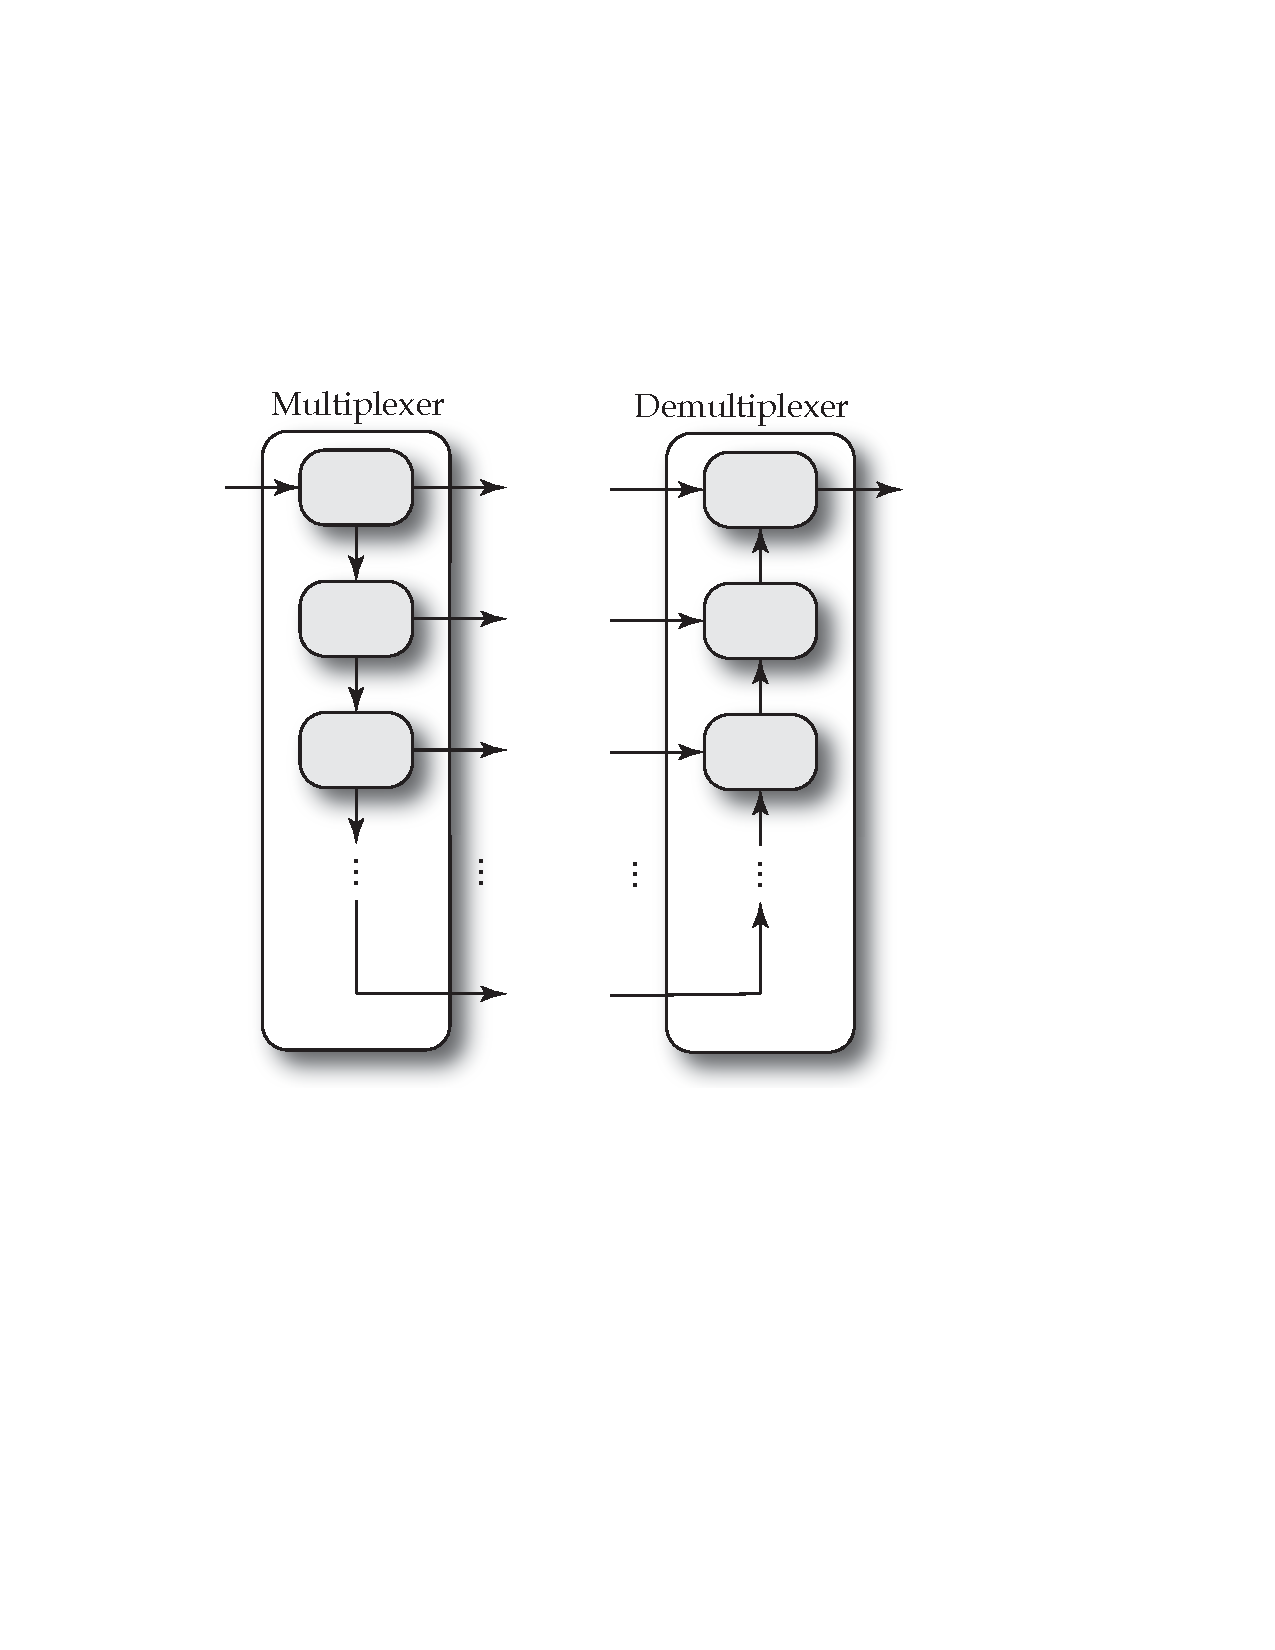
\includegraphics[width=0.85\columnwidth]{linear_multiplexer}
\caption{Linear multiplexers (left) and demultiplexers (right) may be constructed from a linear chain of two-port switches (grey boxes), cascading into one another. These switch a single optical channel between $n$ ports. The total resource requirements are \mbox{$n-1$} two-port switches. The optical depth ranges from $1$ (for the first port) to \mbox{$n-1$} (for the final port).} \label{fig:linear_multiplexer} \index{Linear multiplexers \& demultiplexers}
\end{figure}

\begin{figure}[!htb]
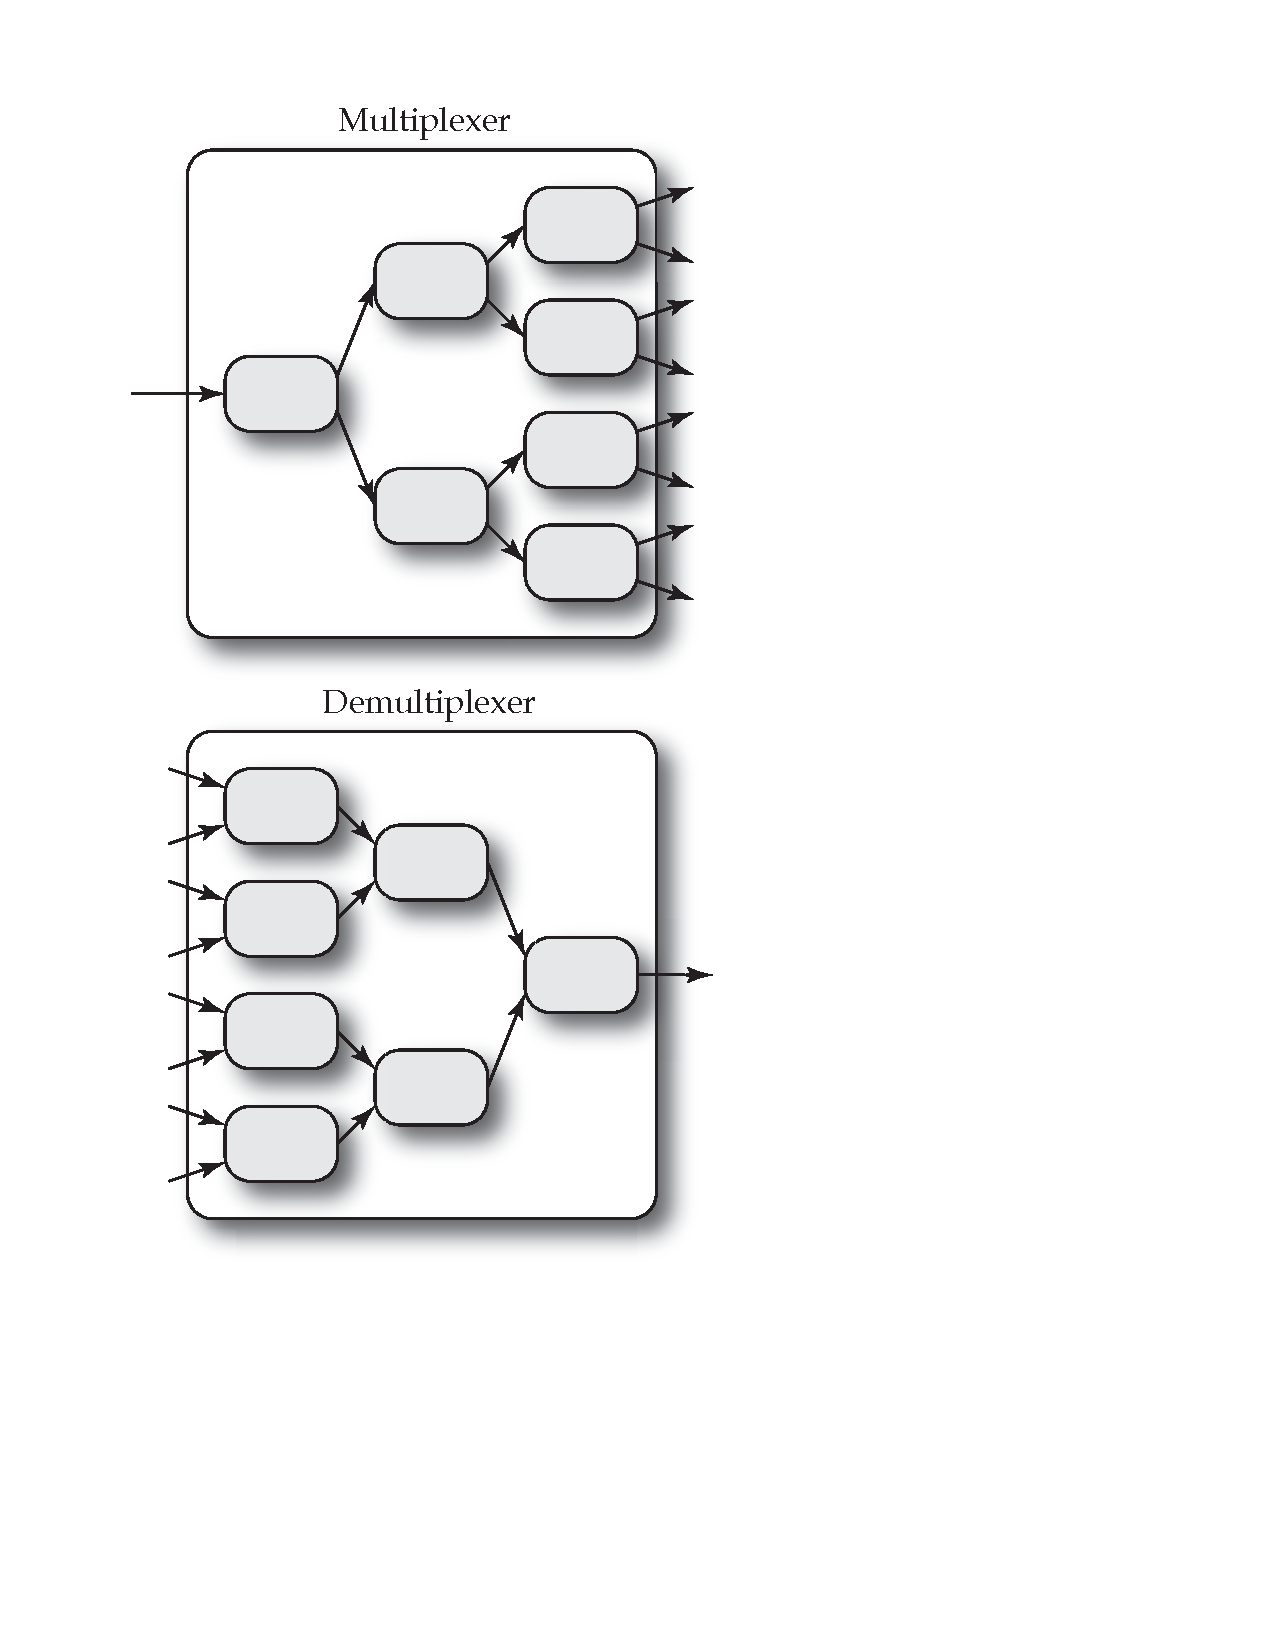
\includegraphics[width=0.7\columnwidth]{pyramid_multiplexer}
\caption{Pyramid multiplexers (top) and demultiplexers (bottom) decompose the multiplexing into a binary tree-structure of two-port switches (grey boxes), shown here for the case of \mbox{$n=8$} ports. For $n$ ports, all optical paths observe an optical depth of \mbox{$d=\mathrm{log}_2(n)$} two-port switches, of which there are \mbox{$n-1$} in total.} \label{fig:pyramid_multiplexer} \index{Pyramid multiplexers \& demultiplexers}
\end{figure}

%
% Single-Channel Multi-Port Switches
%

\subsubsection{Single-channel multi-port switches} \index{Single-channel multi-port switches}

The multiplexers and demultiplexers route between one port and $n$ ports. In the more general and useful case, we wish to route between $n$ inputs and $n$ outputs. If we only require one active channel at a given time, such a router may be trivially constructed from an $n$-port multiplexer connected to and $n$-port demultiplexer, as shown in Fig.~\ref{fig:single_channel_multi_port_switch}. Here the demultiplexer chooses one of the input modes to route to its single output, which then feeds into the multiplexer to fan it out to the desired output. The multiplexers/demultiplexers could be implemented using either of the aforementioned layouts, yielding a total resource count of,
\begin{align}
	N_\mathrm{s} = 2n-3,
\end{align}
two-port switches\footnote{Note that the multiplexer and demultiplexer each require \mbox{$2(n-1)$} two-port switches, but one of the central ones adjoining the multiplexer and demultiplexer is redundant and may be eliminated, reducing the number of two-port switches to \mbox{$2n-3$}.}.

\begin{figure}[!htb]
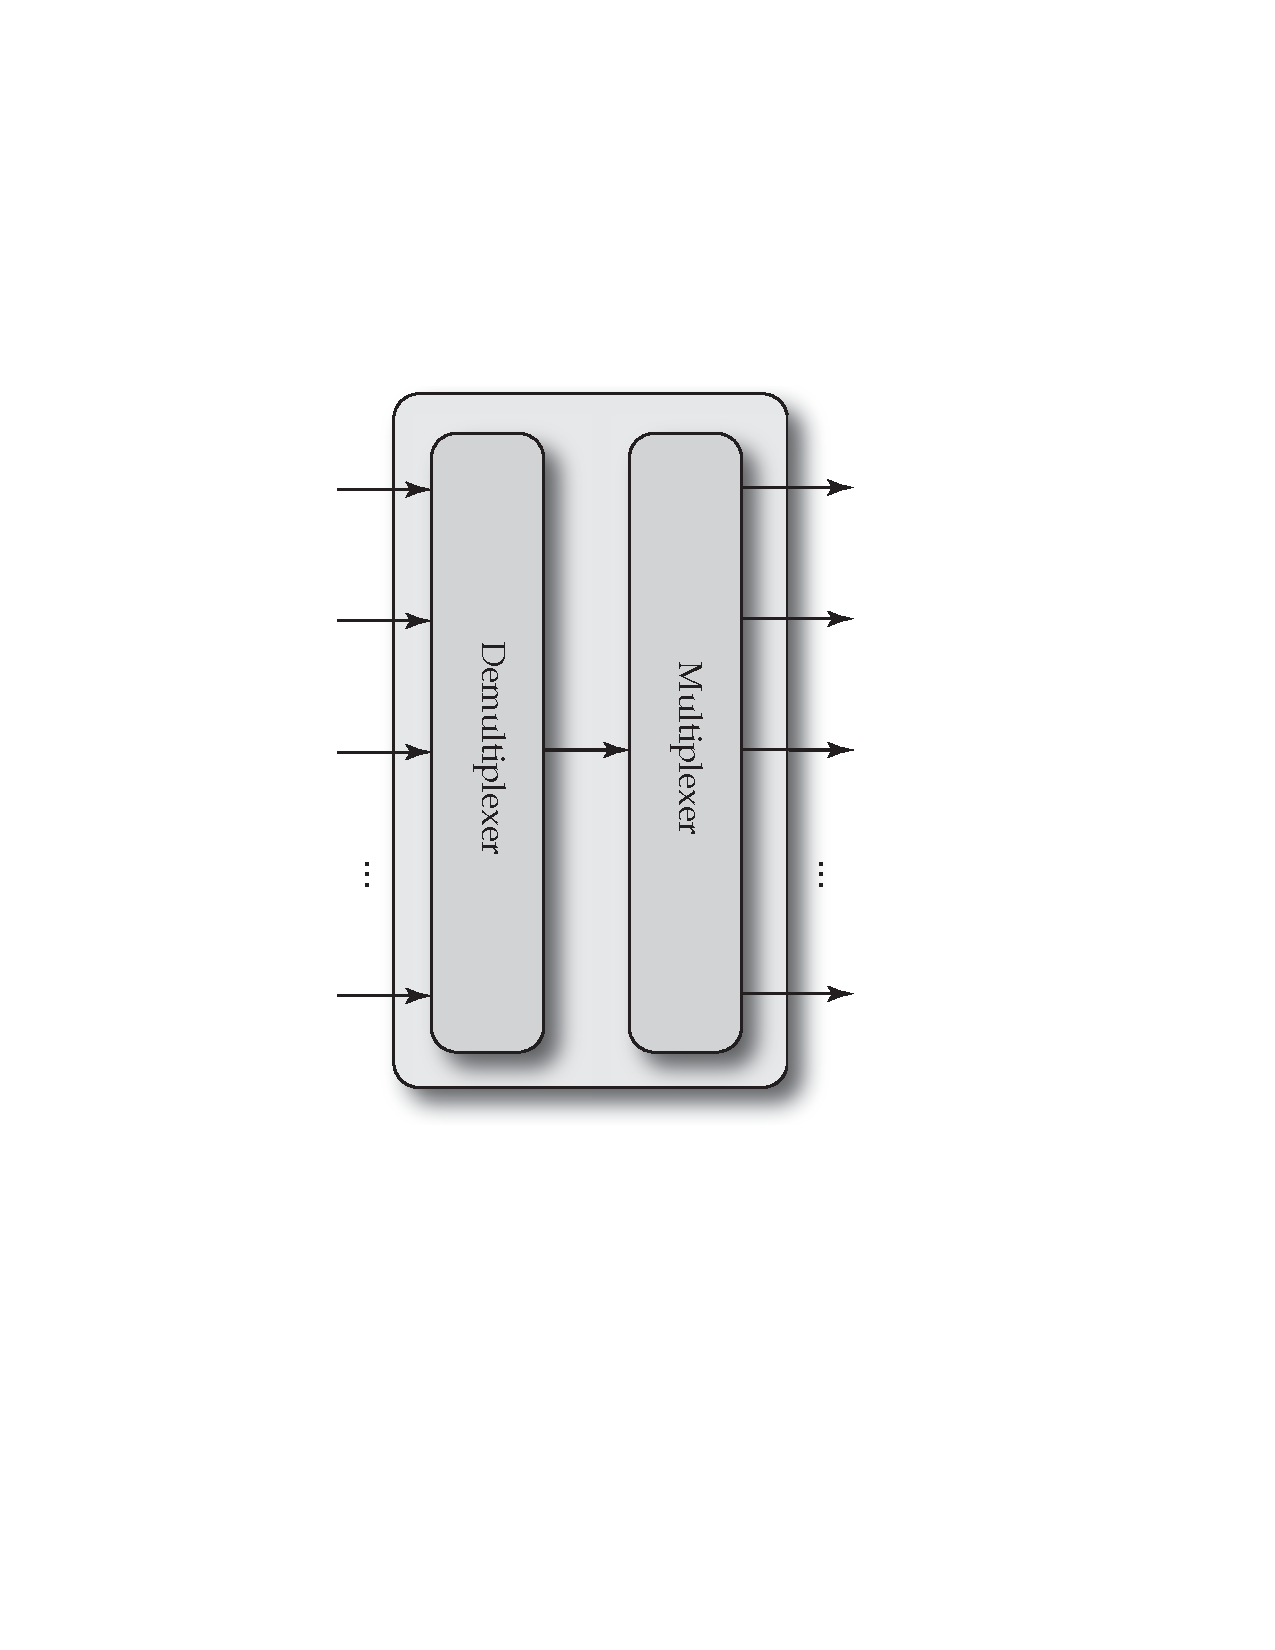
\includegraphics[width=0.75\columnwidth]{single_channel_multi_port_switch}
\caption{A single-channel multi-port switch may be constructed by demultiplexing the $n$ input ports to a single port, routing the desired input channel to that port, before multiplexing it back out to the desired output port. This allows an arbitrary input to be routed to an arbitrary output, but only one channel at a time. This requires \mbox{$2n-3$} two-port switches in total.} \label{fig:single_channel_multi_port_switch} \index{Single-channel multi-port switches}	
\end{figure}

%
% Multi-Channel Multi-Port Switches
%

\subsubsection{Multi-channel multi-port switches} \index{Multi-channel multi-port switches}

The single-channel multi-port switch enables switching between an arbitrary number of input/output ports, but suffers that it can only route a single channel at a time. The most general scenario to consider is multi-channel multi-port switching, which implements an arbitrary permutation between $n$ inputs and $n$ outputs. That is, all $n$ ports may be routing active channels, enabling simultaneous routing of multiple data-flows.

Such a switch may be constructed from a staggered, rectangular lattice of two-port switches, as shown in Fig.~\ref{fig:multi_channel_multi_port_switch}. It is easy to see upon inspection that optical paths exist between every input/output pair of ports. The total resource count for this device is,
\begin{align}
N_\mathrm{s} = \left\lceil \frac{n^2}{2}\right\rceil - n + 1,
\end{align}
two-port switches.

The operation implemented by this device can therefore be expressed as,
\begin{align}
	\left(\begin{matrix}{}
  		\hat{b}^\dag_1 \\
  		\hat{b}^\dag_2 \\
  		\vdots \\
  		\hat{b}^\dag_m
\end{matrix}\right)=\sigma\cdot\left(\begin{matrix}{}
  		\hat{a}^\dag_1 \\
  		\hat{a}^\dag_2 \\
  		\vdots \\
  		\hat{a}^\dag_m
\end{matrix}\right),
\end{align}
where \mbox{$\sigma\in S_m$} is an arbitrary element of the symmetric group (i.e a permutation matrix), and $\hat{a}_i^\dag$ ($\hat{b}_i^\dag$) are the input (output) photonic creation operators.

\begin{figure}[!htb]
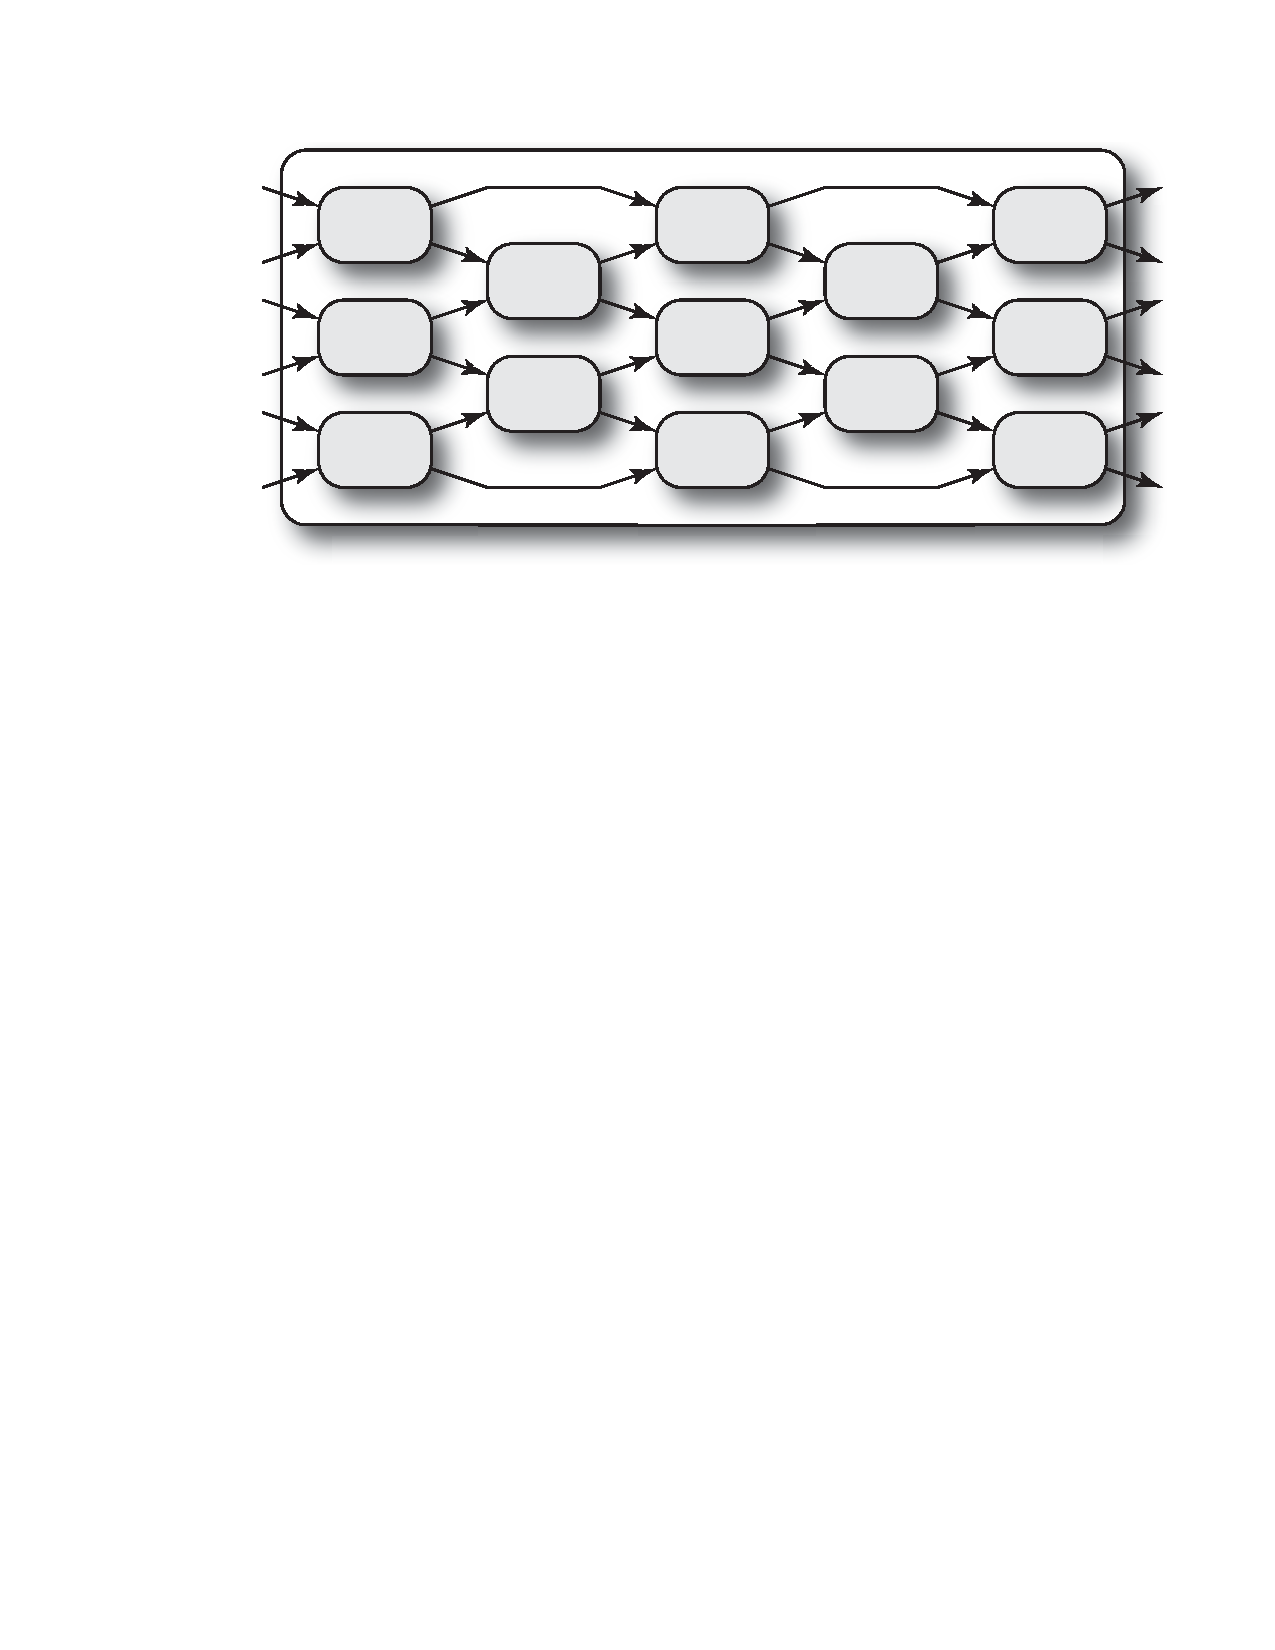
\includegraphics[width=\columnwidth]{multi_channel_multi_port_switch}
\caption{A completely general multi-channel multi-port switch may be constructed using a staggered grid of two-port switches (grey boxes), shown here for \mbox{$n=6$} ports. This allows the implementation of an arbitrary permutation between input and output ports, enabling all $n$ channels to be simultaneously utilised and routed across distinct input-to-output routes. This requires \mbox{$\left\lceil \frac{n^2}{2}\right\rceil - n + 1$} two-port switches in total.} \label{fig:multi_channel_multi_port_switch} \index{Multi-channel multi-port switches}	
\end{figure}

Note that this decomposition is more favourable than the completely general Reck \emph{et al.} decomposition presented in Fig.~\ref{fig:LO_archs}(a), since the circuit is balanced, with (almost!) identical optical depths across all input-to-output paths.

%
% Mechanical Switches
%

\subsection{Mechanical switches}

Most obviously, optical switching could be performed mechanically, by physically displacing fibre endpoints, directing them towards different routes. Such switches have found use in other areas, but are not particularly appropriate for quantum information processing applications, as they are extremely slow compared to electro- or acousto-optic technologies. Certainly, mechanical switching would not be applicable to optical fast-feedforward, such as that required by optical quantum computing, on the order of nanoseconds.

A second disadvantage of mechanical switches is that the introduction of moving parts into quantum optics protocols makes optical stabilisation extremely challenging. The mechanical control required to preserver wavelength-level coherence, for example, is effectively ruled out by moving parts.

%
% Optical Stability In Quantum Networks
%

\section{Optical stability in quantum networks} \label{sec:opt_stab} \index{Optical stability}

Given that communications links in quantum networks are expected to be optical, an issue of central importance is optical stability when signals from remote sources interfere or interact with local quantum states. For example, in an entanglement swapping protocol (Sec.~\ref{sec:swapping}) forming a part of a quantum repeater network (Sec.~\ref{sec:rep_net}), if the entangling operation between the remotely prepared qubits suffers errors, so too will the prepared distributed entangled state.

If we consider the simplest scenario of employing a PBS (Sec.~\ref{sec:bell_proj}) to implement the entangling operation in the polarisation degree of freedom, photon distinguishability in the form of mode-mismatch (Sec.~\ref{sec:MM_error}) will undermine quantum interference, thereby reducing the entangling power of the gate. Similar observations apply to many other protocols involving entangling measurements, or multi-photon interference more generally.

In present-day laboratories, mode-mismatch and photon-distinguishability can be controlled with exceptionally high fidelity. However, in the networking context this is likely to not be so easy, since perfectly aligning states emanating over long-distance communications channels, which we do not have exquisite control over in a well-controlled laboratory setting, is going to be a somewhat unpredictable and time-varying technological challenge.

Such processes are likely to arise in a multitude of ways, including, but certainly not limited to:
\begin{itemize}
	\item Optical fibre: slight variations in temperatures induce refractive index changes, or changes in physical dimension, resulting in temporal displacements of optical wave-packets.
	\item Satellite: precise knowledge of the distance to a rapidly moving target, at the scale of photon wave-packets, is an extremely daunting prospect.
	\item Free space (including via satellite): unpredictable temperature and pressure fluctuations in the atmosphere cause unpredictable variations in the speed of light.
\end{itemize}

For these inevitable reasons, it is important to understand the susceptibility of different network protocols to optical stability. 

There are two dominant forms of photonic interference that must be considered, each with quite distinct behaviours under the influence of optical instability. These are:
\begin{itemize}	
	\item Hong-Ou-Mandel (HOM) interference (Sec.~\ref{sec:HOM_inter}):  interference between two distinct photons at a beamsplitter.
	\item Mach-Zehnder (MZ) interference (Sec.~\ref{sec:MZ_inter}): self-interference of a single-photon traversing multiple paths in superposition within an interferometer.
\end{itemize}

%
% Photon Wave-Packets
%

\subsection{Photon wave-packets} \index{Wave-packets}

Before describing optical interference in detail, we must first formalise a definition for the optical wave-packets we will be dealing with. We will assume wave-packets with Gaussian temporal envelope of width $\sigma$, frequency-shifted by some carrier frequency $\omega_0$. The temporal distribution function is then,
\begin{align} \label{eq:wavepacket_modulated}
\psi(t) = \sqrt[4]{\frac{2}{\sigma\pi}}e^{-\frac{t^2}{\sigma}-i\omega_0t},
\end{align}
with associated mode-operator $\hat{A}^\dag_\psi$ (Sec.~\ref{sec:spatio_temporal}). This wave-packet is normalised such that,
\begin{align}
|\bra{0} \hat{A}_\psi \hat{A}_\psi^\dag \ket{0}|^2 = \int_{-\infty}^\infty |\psi(t)|^2 \, dt = 1.
\end{align}

Of course the temporal envelope needn't be Gaussian in general, and could take any other form, subject to normalisation. In Fig.~\ref{fig:HOM_vs_MZ} we illustrate the two main features of this representation: the temporal envelope, and the underlying carrier frequency that it modulates.

In real-world scenarios we are likely to encounter carrier frequencies sufficiently large that oscillations at the carrier frequency level are far more rapid than that of the temporal envelope. For this simple reason, it is to be expected that interference dependent only on $\sigma$ will be far more robust against temporal instability than interference dependent on $\omega_0$.

\begin{figure}[!htb]
	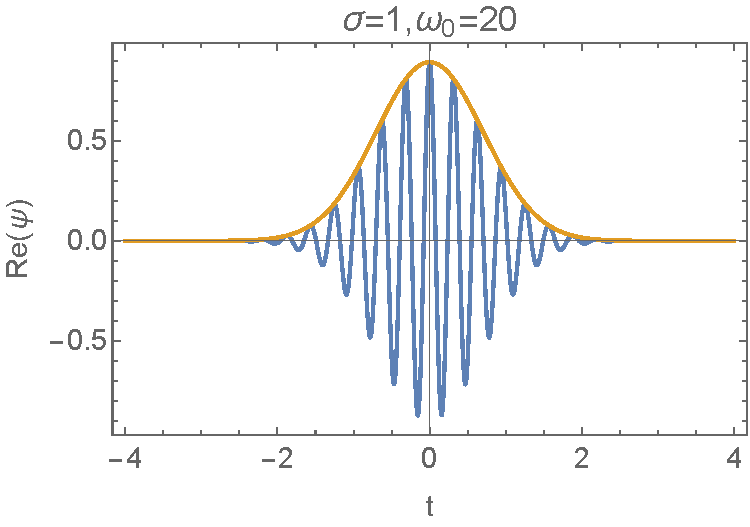
\includegraphics[width=\columnwidth]{wavepacket} \\
	\caption{(top) A photonic wave-packet of the form of Eq.~(\ref{eq:wavepacket_modulated}), with Gaussian temporal envelope of width $\sigma$ (orange), shifted by a carrier frequency $\omega_0$ (blue).} \label{fig:HOM_vs_MZ}
\end{figure}

%
% Mach-Zehnder Interference
%

\subsection{Mach-Zehnder interference} \index{Mach-Zehnder (MZ) interference} \label{sec:MZ_inter}

Mach-Zehnder (MZ) interference is the interference of a photon or coherent state with itself in a two-mode interferometer constructed from two 50:50 beamsplitters in series, as shown in Fig.~\ref{fig:MZ_inter}(top). This is MZ interference in its simplest form, which can of course be generalised to more complex networks involving self-interference across multiple optical paths.

Within the interferometer is a time-delay, $\tau$, which acts as a temporal mismatch between the two optical paths. 

\begin{figure}[!htb]
	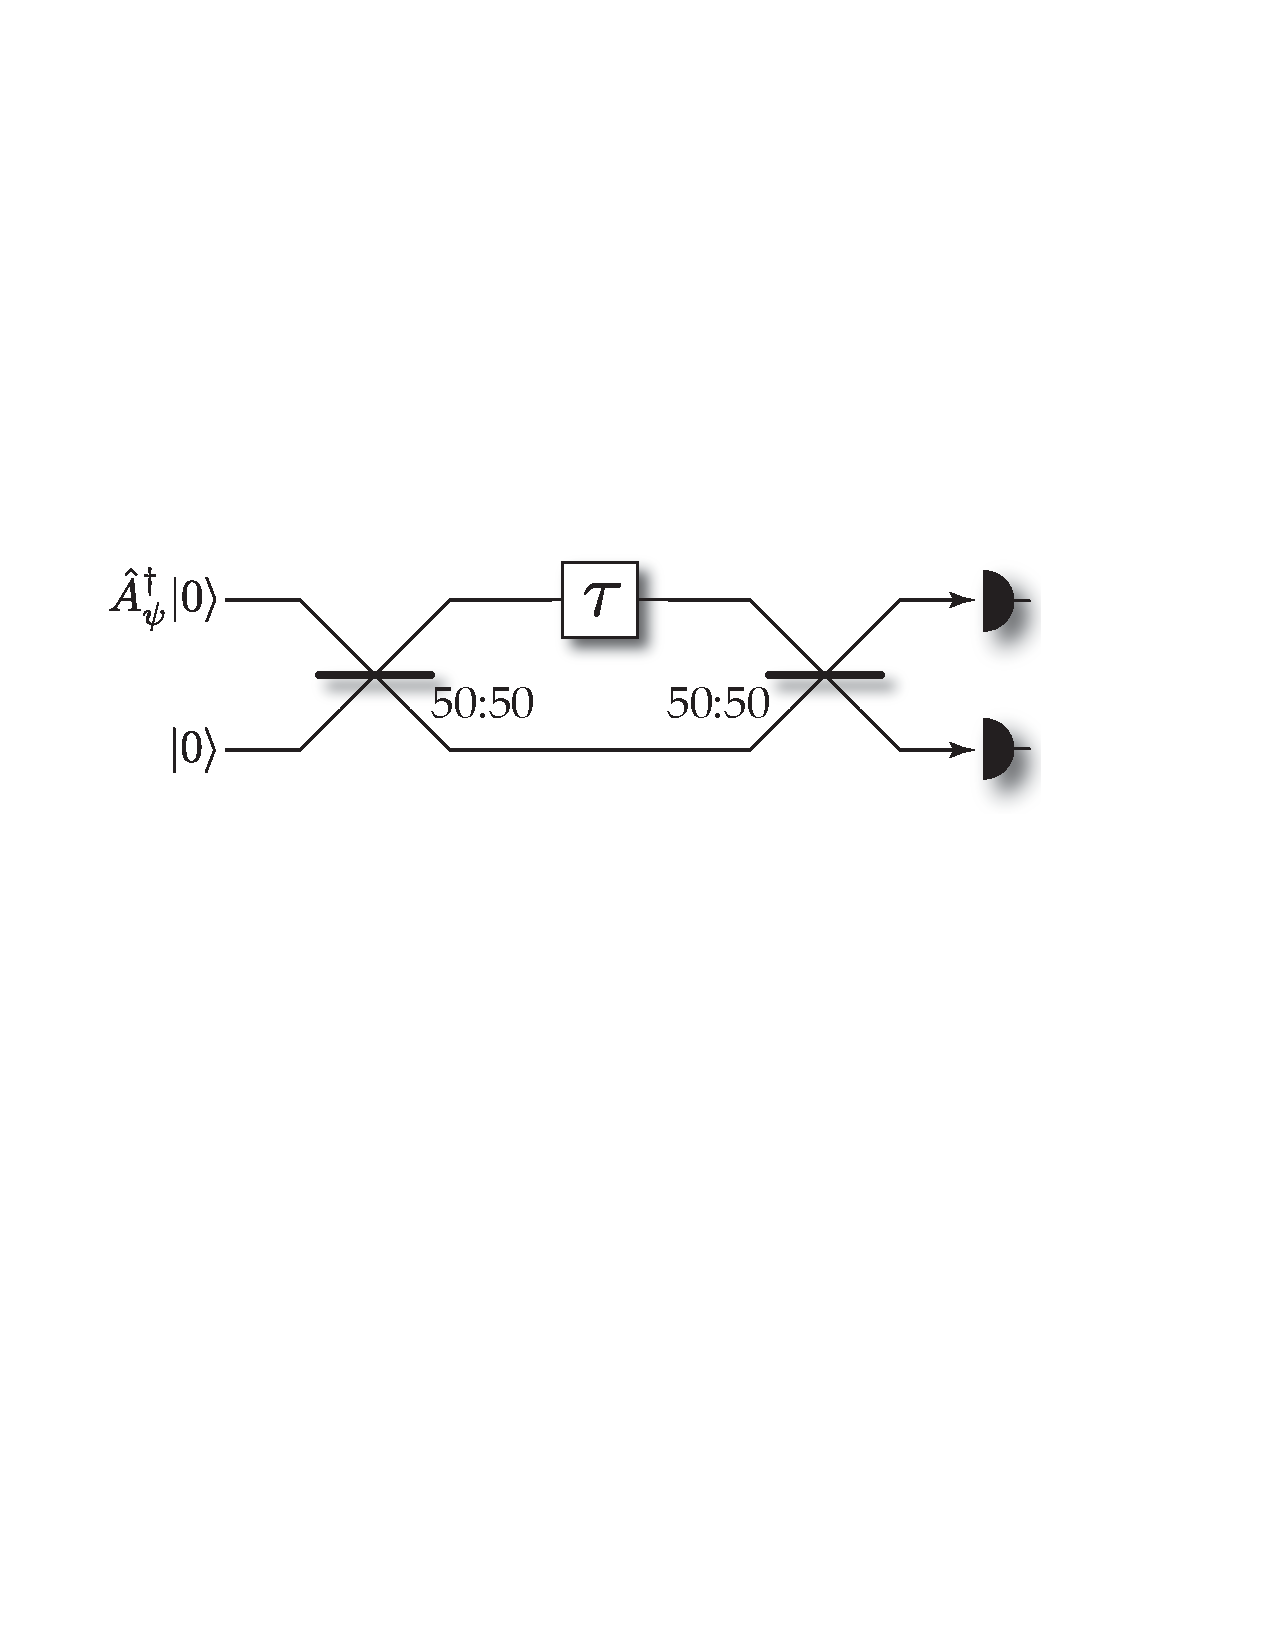
\includegraphics[width=\columnwidth]{MZ_setup} \\
	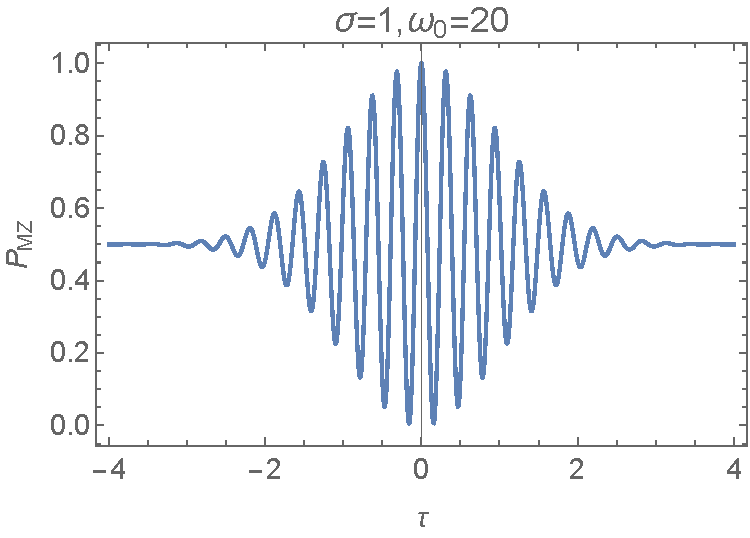
\includegraphics[width=\columnwidth]{MZ}
	\caption{Mach-Zehnder self-interference of a single photon. (top) Layout of the interferometer. The photon is subject to a time-delay $\tau$ within only the upper arm of a balanced interferometer, comprising two 50:50 beamsplitters. (bottom) Interference fringe $P_\text{MZ}(\tau)$ as a function of the time-delay. The interference is sensitive at the scale of the photon wavelength, (blue) in Fig.~\ref{fig:HOM_vs_MZ}.} \label{fig:MZ_inter}
\end{figure}

Let us calculate explicitly the evolution of a single-photon through this device, beginning with a photon described by mode operator $\hat{A}^\dag_\psi$\index{Mode operators} (Sec.~\ref{sec:spatio_temporal}), with the temporal distribution function from Eq.~(\ref{eq:wavepacket_modulated}). We have,
\begin{align}
	\ket\psi_\text{in} &= \hat{A}^\dag_\psi \ket{0,0} \nonumber \\
	&\underset{\text{BS}}{\to} \frac{1}{\sqrt{2}} [\hat{A}^\dag_\psi + \hat{B}^\dag_\psi] \ket{0,0} \nonumber \\
	&\underset{\tau}{\to} \frac{1}{\sqrt{2}} [\hat{A}^\dag_{\psi-\tau} + \hat{B}^\dag_\psi] \ket{0,0} \nonumber \\
	&\underset{\text{BS}}{\to} \frac{1}{2} [\hat{A}^\dag_{\psi-\tau} + \hat{B}^\dag_{\psi-\tau} + \hat{A}^\dag_\psi - \hat{B}^\dag_\psi] \ket{0,0} \nonumber \\
	&\underset{\text{PS}}{\to} \frac{1}{2} [\hat{A}^\dag_{\psi-\tau} + \hat{A}^\dag_\psi] \ket{0,0} \nonumber \\
	&= \frac{1}{2} \int_{-\infty}^\infty [\psi(t) + \psi(t-\tau)] \hat{a}^\dag(t)\,dt,
\end{align}
where BS denotes the evolution implemented by a 50:50 beamsplitter, and PS denotes post-selecting upon detecting a single-photon in the first output mode.

We now characterise the operation of the device in terms of the probability of detecting the photon in the first output mode,
\begin{align}
P_\text{MZ}(\tau) &= \frac{1}{4} \int_{-\infty}^\infty |\psi(t) + \psi(t-\tau)|^2 \,dt \nonumber \\
&= \frac{1}{2} \left[ 1 + e^{-\frac{\tau^2}{2\sigma}}\text{cos}(\omega_0\tau) \right].
\end{align}
These dynamics are shown in Fig.~\ref{fig:MZ_inter}(bottom). There are two key features in the behaviour of $P_\text{MZ}(\tau)$. First, there is a slowly varying Gaussian term. Second, the Gaussian term modulates a rapidly oscillating sinusoidial term associated with the carrier frequency. This implies that $\tau$ on the order of the photon's wavelength dominates the measurement dynamics, making it extremely sensitive to temporal instability.

%
% Hong-Ou-Mandel Interference
%

\subsection{Hong-Ou-Mandel interference} \index{Hong-Ou-Mandel (HOM) interference} \label{sec:HOM_inter}

In Hong-Ou-Mandel (HOM) interference, there is no self-interference as per MZ, but rather interference between two independent but indistinguishable photons. The interference takes place at a single 50:50 beamsplitter, with a temporal delay in one input mode modelling temporal instability. The model is shown in Fig.~\ref{fig:HOM_inter}(top).

\begin{figure}[!htb]
	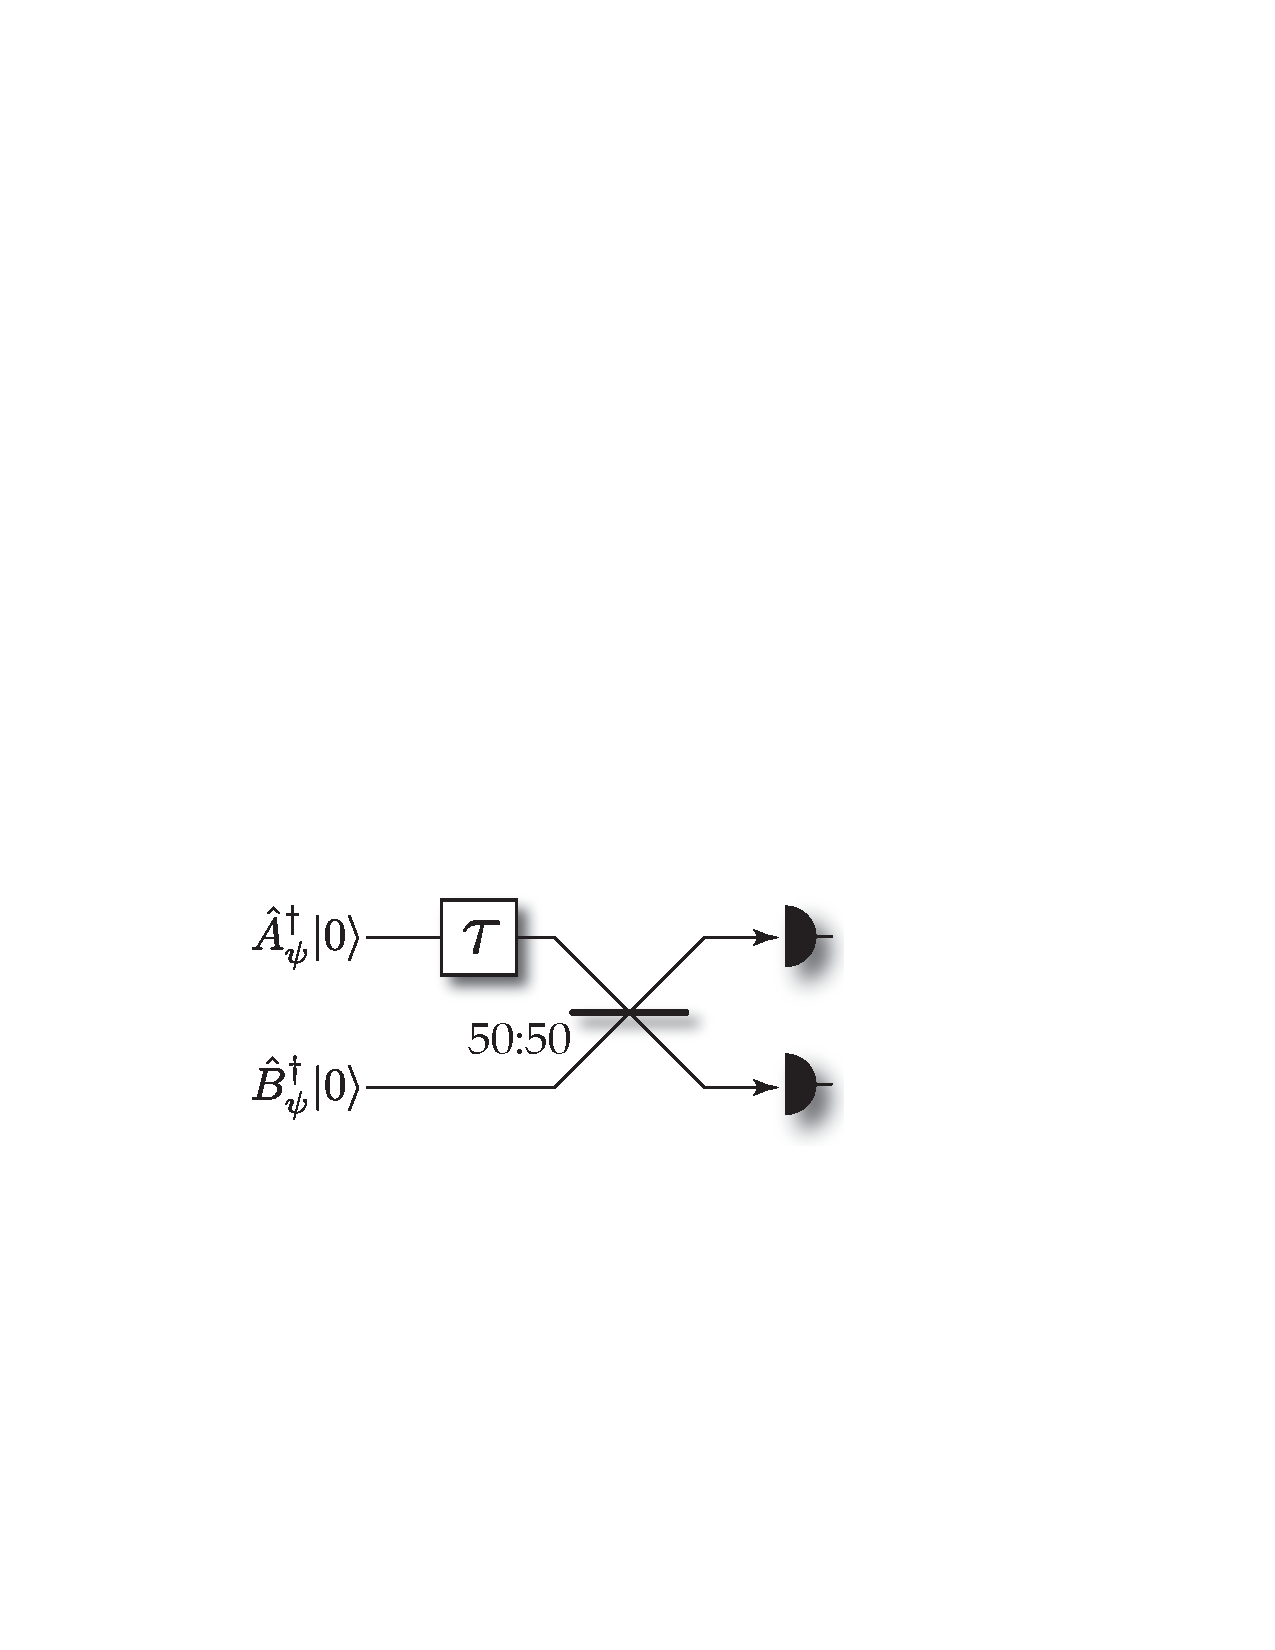
\includegraphics[width=0.63\columnwidth]{HOM_setup} \\
	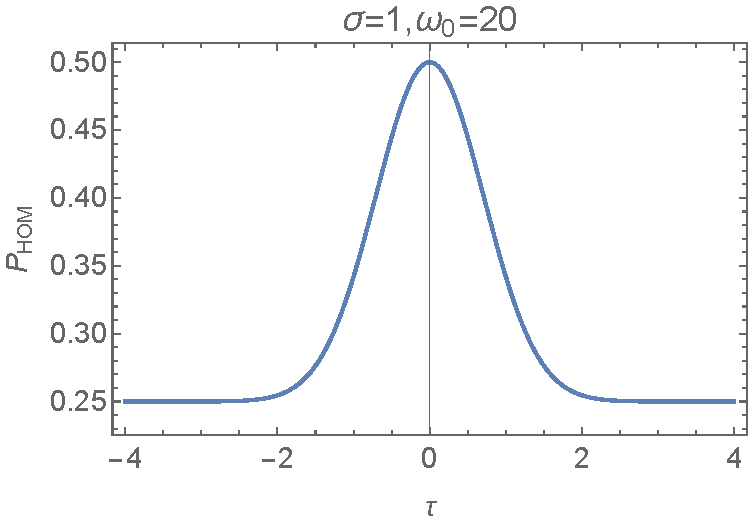
\includegraphics[width=\columnwidth]{HOM}
	\caption{Hong-Ou-Mandel interference between two independent photons, $A$ and $B$. (top) Layout of the interferometer. Two photons given by mode operators $\hat{A}^\dag$ and $\hat{B}^\dag$\index{Mode operators} (Sec.~\ref{sec:spatio_temporal}), both with temporal distribution function $\psi(t)$, interfere at a 50:50 beamsplitter, where mode $A$ is first subject to a time-delay $\tau$. (bottom) Interference fringe $P_\text{HOM}(\tau)$ as a function of the time-delay. The fringe is only sensitive at the scale of the wave-packet envelope, (orange) in Fig.~\ref{fig:HOM_vs_MZ}.} \label{fig:HOM_inter}
\end{figure}

Performing the same evaluation of the evolution of the system as before, we obtain,
\begin{align}
	\ket\psi_\text{in} &= \hat{A}^\dag_\psi \hat{B}^\dag_\psi \ket{0,0} \nonumber \\
	&\underset{\tau}{\to} \hat{A}^\dag_{\psi-\tau} \hat{B}^\dag_\psi \ket{0,0} \nonumber \\
	&\underset{BS}{\to} \frac{1}{2} [\hat{A}^\dag_{\psi-\tau} + \hat{B}^\dag_{\psi-\tau}] [\hat{A}^\dag_\psi - \hat{B}^\dag_\psi] \ket{0,0} \nonumber \\
	&\underset{PS}{\to} \frac{1}{2} \hat{A}^\dag_\psi \hat{A}^\dag_{\psi-\tau} \ket{0,0} \nonumber \\
	&= \frac{1}{2} \int_{-\infty}^\infty \int_{-\infty}^\infty \psi(t)\psi(t'-\tau)\hat{a}^\dag(t)\hat{a}^\dag(t')\,dt\,dt'.
\end{align}

We then characterise the operation of the device in terms of the probability of detecting both photons in the first output mode (photon bunching),
\begin{align}
	P_\text{HOM}(\tau) &= \frac{1}{4} \left[1 + \left|\int_{-\infty}^\infty \psi(t)\psi(t-\tau)^*\,dt\right|^2 \right] \nonumber \\
	&= \frac{1}{4}\left[ 1 + e^{-\frac{\tau^2}{\sigma}} \right].
\end{align}
These dynamics are shown in Fig.~\ref{fig:HOM_inter}(bottom). Now, unlike MZ interference, we observe no dependence on the carrier frequency and its associated rapidly oscillating terms. Rather, operation depends only on the temporal envelop, which exists over a far larger time-scale.

Importantly, unlike MZ interference, HOM interference is not applicable to coherent states, which do not entangle or enter into superposition at beamsplitters. The photon bunching effect is unique to single-photons.

The intuition behind the HOM-dip phenomenon is as follows. We know that for identical, indistinguishable photons, an input photon-pair evolves as,
\begin{align}
\ket{1,1} \underset{BS}{\to} \frac{1}{\sqrt{2}}(\ket{2,0}-\ket{0,2}),
\end{align}
yielding perfect photon-bunching. This bunching effect arises from quantum mechanical interference between the photons. Next imagine that the two photons arrived a long time apart from one another, so long that their wave-packets do not overlap at all. In that instance, the photons do not `see' one another and no quantum interference takes place. Instead, rather than a two-photon quantum interference experiment, we effectively have two independent instances of single-photon experiments, given by,
\begin{align}
\ket{1,0} &\underset{BS}{\to} \frac{1}{\sqrt{2}}(\ket{1,0}+\ket{0,1}), \nonumber \\	
\ket{0,1} &\underset{BS}{\to} \frac{1}{\sqrt{2}}(\ket{1,0}-\ket{0,1}).
\end{align}
Note that each of these independent instances obeys the classical statistics of a 50/50 distribution. Combining the two instances using classical probability theory, we now observe a 50\% chance of measuring a coincidence, as opposed to the 0\% chance for true HOM interference.

%
% HOM vs MZ Interference
%

\subsection{HOM vs MZ interference} \index{Mach-Zehnder (MZ) interference}\index{Hong-Ou-Mandel (HOM) interference}\index{Hong-Ou-Mandel vs Mach-Zehnder interference}

Let us now examine the implications of these different types of interference. The key observation was that MZ is far more sensitive to temporal mismatch than HOM, the former at the scale of the photons' wavelength, the latter at the scale of their temporal envelope, which is far larger.

This leads to the immediate conclusion that network protocols relying on HOM interference will be far more robust against temporal instability than those relying on MZ interference. Realistically, it is to be expected that the latter might be impossibly challenging in many contexts, as wavelength-scale stabilisation over long distances seems implausible.

In Table.~\ref{table:summary_inter} we summarise the network protocols discussed in Sec.~\ref{sec:protocols_quant_int} in terms of the types of interference they rely upon. This creates a picture of which are more realistic from a near-term engineering perspective.

\begin{table}[!htb]
	\begin{tabular}{|c|c|}
		\hline
  		Protocol & Interference type \\
  		\hline
  		\hline
  		Cluster state measurement & None \\
   		Quantum anonymous broadcasting & None \\
  		QKD (BB84, E91) & None \\
  		Quantum memory & None \\
  		Quantum process tomography & None \\
  		Quantum state tomography & None \\
  		Random number generation & None \\
  		Separable measurements & None \\
  		Separable state preparation & None \\
  		Optical interfacing & None \\
  		\hline
  		Cluster state preparation (fusion gates) & HOM \\
  		Entanglement purification & HOM \\
  		Entanglement swapping & HOM \\ 
  		Matter qubit entangling operations & HOM \\
  		Partial Bell state measurements & HOM \\
   		Quantum gate teleportation & HOM \\
  		Quantum state teleportation & HOM \\
  		\hline
  		{\sc BosonSampling} & MZ \\
  		General linear optics networks & MZ \\
  		Universal LOQC (KLM) & MZ \\
  		Quantum metrology & MZ \\
  		Quantum walks & MZ \\
    	\hline
	\end{tabular}
	\caption{Summary of the major quantum network protocols presented in Sec.~\ref{sec:protocols_quant_int}, and their required type of interference.}\index{Interferometric requirements}\label{table:summary_inter}
\end{table}

%
% Optical Stabilisation
%

\subsection{Optical stabilisation} \index{Optical stabilisation}

\comment{To do!}

%
% Protocols for the Quantum Internet
%

\section{Protocols for the quantum internet} \label{sec:protocols_quant_int} \index{Protocols for quantum networks}

There are countless applications for the long-distance communication and processing of quantum data. We will outline some of the most notable examples. Broadly, we will begin with discussion of \textit{low-level protocols} that form the primitives upon which other protocols are built. We will then progressively move towards \textit{high-level protocols}, culminating with full \textit{cloud quantum computing}.

Much of the recent experimental progress in quantum technology has been in the area of low-level protocols, although demonstrations of higher-level protocols are rapidly accelerating.

We keep in mind that although throughout this presentation we have been very quantum computing-centric, quantum computing is not the \textit{only} quantum resource worth communicating. In the same way that \textit{digital assets} encompass a broad range of digital systems and information, any aspect of a quantum system -- from a state, to an operation, storage, to a measurement, or anything else -- could be treated as a \textit{quantum asset}\index{Quantum assets}, which, for generality, we would like our quantum networks to be able to handle.

At the lowest physical level, quantum protocols have in common that they involve state preparation, evolution, and measurement as the fundamental primitives upon which more complex protocols are constructed. We consider these primitive resources in detail, before building upon them to consider some of the major elementary quantum protocols that implement tasks of practical interest. All of those discussed here have been subject to extensive experimental investigation and demonstration, which will be summarised in Sec.~\ref{sec:state_of_the_art}. We treat full quantum computation separately in Secs.~\ref{sec:models_QC} \& \ref{sec:archs_QC}, as this is such an involved topic in its own right.

We will employ circuit model diagrams when describing some protocols. The unfamiliar reader may refer to Sec.~\ref{sec:circuit_model} for a very brief introduction to quantum circuits.

%
% State Preparation
%

\subsection{State preparation} \index{State preparation}

The first step in any quantum protocol involves the preparation of some kind of quantum state. Some quantum states are easy and cheap to prepare. Others are complex and costly. Thus, the most fundamental quantum asset that a quantum network must handle is the preparation and communication of quantum states.

A state prepared by Bob and sent to Alice might be prepared in isolation, or it might be entangled with a much larger system held by Charlie, that Alice does not have full access to. In that case, it would be impossible for Alice to prepare the state on her own, unless she were to first establish a relationship with Charlie. Alternately, maybe Alice just isn't very well-resourced, and can't do much on her own. The ability to let someone else prepare her desired quantum states for her would be highly appreciated.

Given the emphasis on quantum optics in quantum networking, it should be noted that optical quantum state engineering has broad applications, but can be very challenging in general. Single-photon state engineering, for example, finds ubiquitous applications in quantum information processing protocols, and has become commonplace. Most notably, linear optics quantum computing (Sec.~\ref{sec:KLM_univ}), and some quantum metrology protocols (Sec.~\ref{sec:metrology}) rely on single-photon state preparation. `Push-button' (i.e on-demand) single-photon sources would be a prized asset to many undergraduate experimentalists, were they able to afford them. But with access to the quantum internet, they could purchase single photons from another better-resourced lab, with QoS constraints guaranteed by QTCP.

The QTCP protocol is ideally suited to facilitating this kind of transaction. With the use of efficiency and purity cost metrics, QoS guarantees could be established for the efficiency and purity of a licensed single-photon source. In the case of single photons, the dephasing metric is irrelevant, since photon-number states are phase-invariant. This is an elegant example of the value of the versatility of having the QTCP protocol track multiple cost metrics for quantum packets, since different metrics will be of relevance to different messages. Were the message a coherent state, $\ket\alpha$, on the other hand, dephasing would be of utmost importance, whereas loss would be less critical, as lossy coherent states remain as coherent states and retain their coherence.

We see that even the most basic primitive in quantum technologies -- state preparation -- already brings with it much to take into consideration when designing quantum networks. However, the QTCP protocols we described earlier are versatile enough to be capable of mediating their distribution across quantum networks, whilst providing QoS guarantees.

%
% Coherent States
%

\subsubsection{Coherent states} \label{sec:coherent_states} \index{Coherent state preparation}

Coherent states (Sec.~\ref{sec:coherent_state_enc}), although not strictly \textit{quantum} states, nonetheless find broad applications in quantum protocols, for example as the pump for SPDC\index{Spontaneous parametric down-conversion (SPDC)} sources (Sec.~\ref{sec:single_phot_src}), or as a phase-reference for homodyne detection (Sec.~\ref{sec:homodyne}). Coherent states are rather trivial to prepare, as they are closely approximated by laser sources. Despite their triviality, high quality lasers can nonetheless become very expensive, large, and inaccessible to the not-so-well-resourced end-user. It is not uncommon for laser sources in contemporary labs to be valued in the \$100k's.

%
% Single-Photons
%

\subsubsection{Single-photons} \label{sec:single_phot_src} \index{Single-photon state preparation}

Single-photon sources (Sec.~\ref{sec:single_phot_enc}) \cite{bib:Oxborrow05} are of particular interest, as a foundational building block in many optical quantum information processing applications, such as linear optics quantum computing (Sec.~\ref{sec:KLM_univ}) and quantum key distribution (Sec.~\ref{sec:QKD}).

The most common approach to preparing single-photon states is via heralded SPDC\index{Spontaneous parametric down-conversion (SPDC)} \cite{bib:URen03, bib:URen05}, whereby a coherent pump source is down-converted into two-mode photon-pairs via a second-order non-linear crystal with interaction Hamiltonian of the form,
\begin{align}
\hat{H}_\text{SPDC} = \xi(\hat{a}_p\hat{a}_s^\dag\hat{a}_i^\dag + \hat{a}_p^\dag\hat{a}_s\hat{a}_i),
\end{align}
where $\xi$ is the interaction strength, and $\hat{a}_p$, $\hat{a}_s$ and $\hat{a}_i$ are the photonic annihilation operators for the pump (input), and \textit{signal} and \textit{idler} (output) modes respectively. This has the clear intuitive interpretation as the coherent exchange of photon-pairs in the output modes with photons in the coherent pump.

Specifically, a two-mode SPDC state takes the form,
\begin{align}
\ket\psi_\text{SPDC} = \sqrt{1-\chi^2} \sum_{n=0}^\infty \chi^n \ket{n}_s\ket{n}_i,
\end{align}
where $\chi$ is the squeezing parameter, a function of the pump-power and properties of the crystal. The layout is shown in Fig.~\ref{fig:SPDC_source}.

\begin{figure}[!htb]
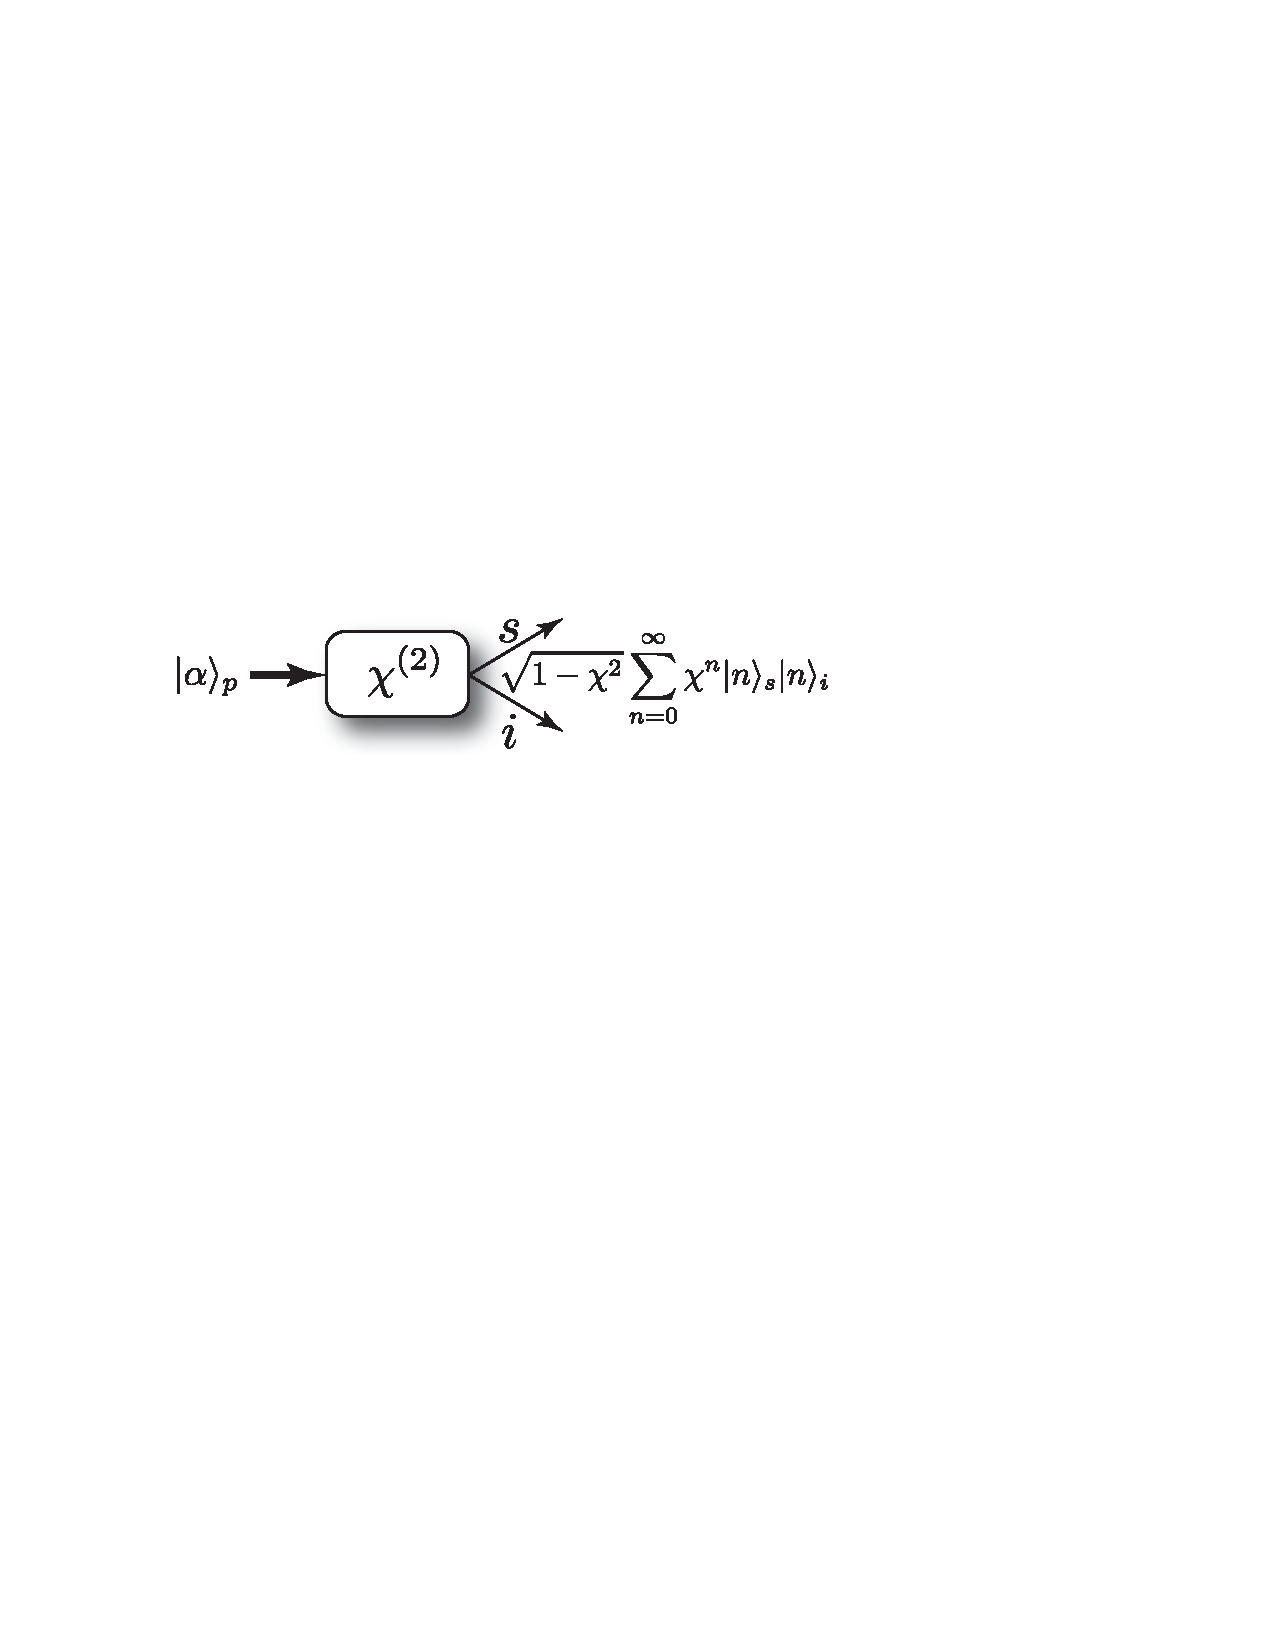
\includegraphics[width=0.9\columnwidth]{SPDC_source}
\caption{Layout of an SPDC single-photon source. A second-order non-linear crystal is pumped with a coherent state (i.e laser source), yielding a two-mode output state with perfect photon-number correlation between the two modes. Then, post-selecting upon detecting a single photon in one mode in principle guarantees a single photon in the other.} \label{fig:SPDC_source}
\end{figure}

Applying the single-photon projector, \mbox{$\ket{1}\bra{1}$}, to the first mode yields the single-photon state in the other, up to normalisation, which reflects the inherent non-determinism. The preparation success probability is derived from the amplitude of the \mbox{$n=1$} term as,
\begin{align} \label{eq:SPDC_p_prep}
P_\text{prep}=\chi^2(1-\chi^2),
\end{align}
assuming ideal photo-detection. Thus, the perfect photon-number correlation enables heralded preparation of states with exactly one photon in principle.

Transitioning from heralded state preparation to quasi-deterministic state preparation may then be achieved by operating a bank of such sources in parallel, and multiplexing their outputs, such that when all sources are triggered simultaneously, if any one succeeds, the respective single photon is routed to the desired output mode \cite{???}, as shown in Fig.~\ref{fig:SPDC_multiplexing_arch}.

\begin{figure}[!htb]
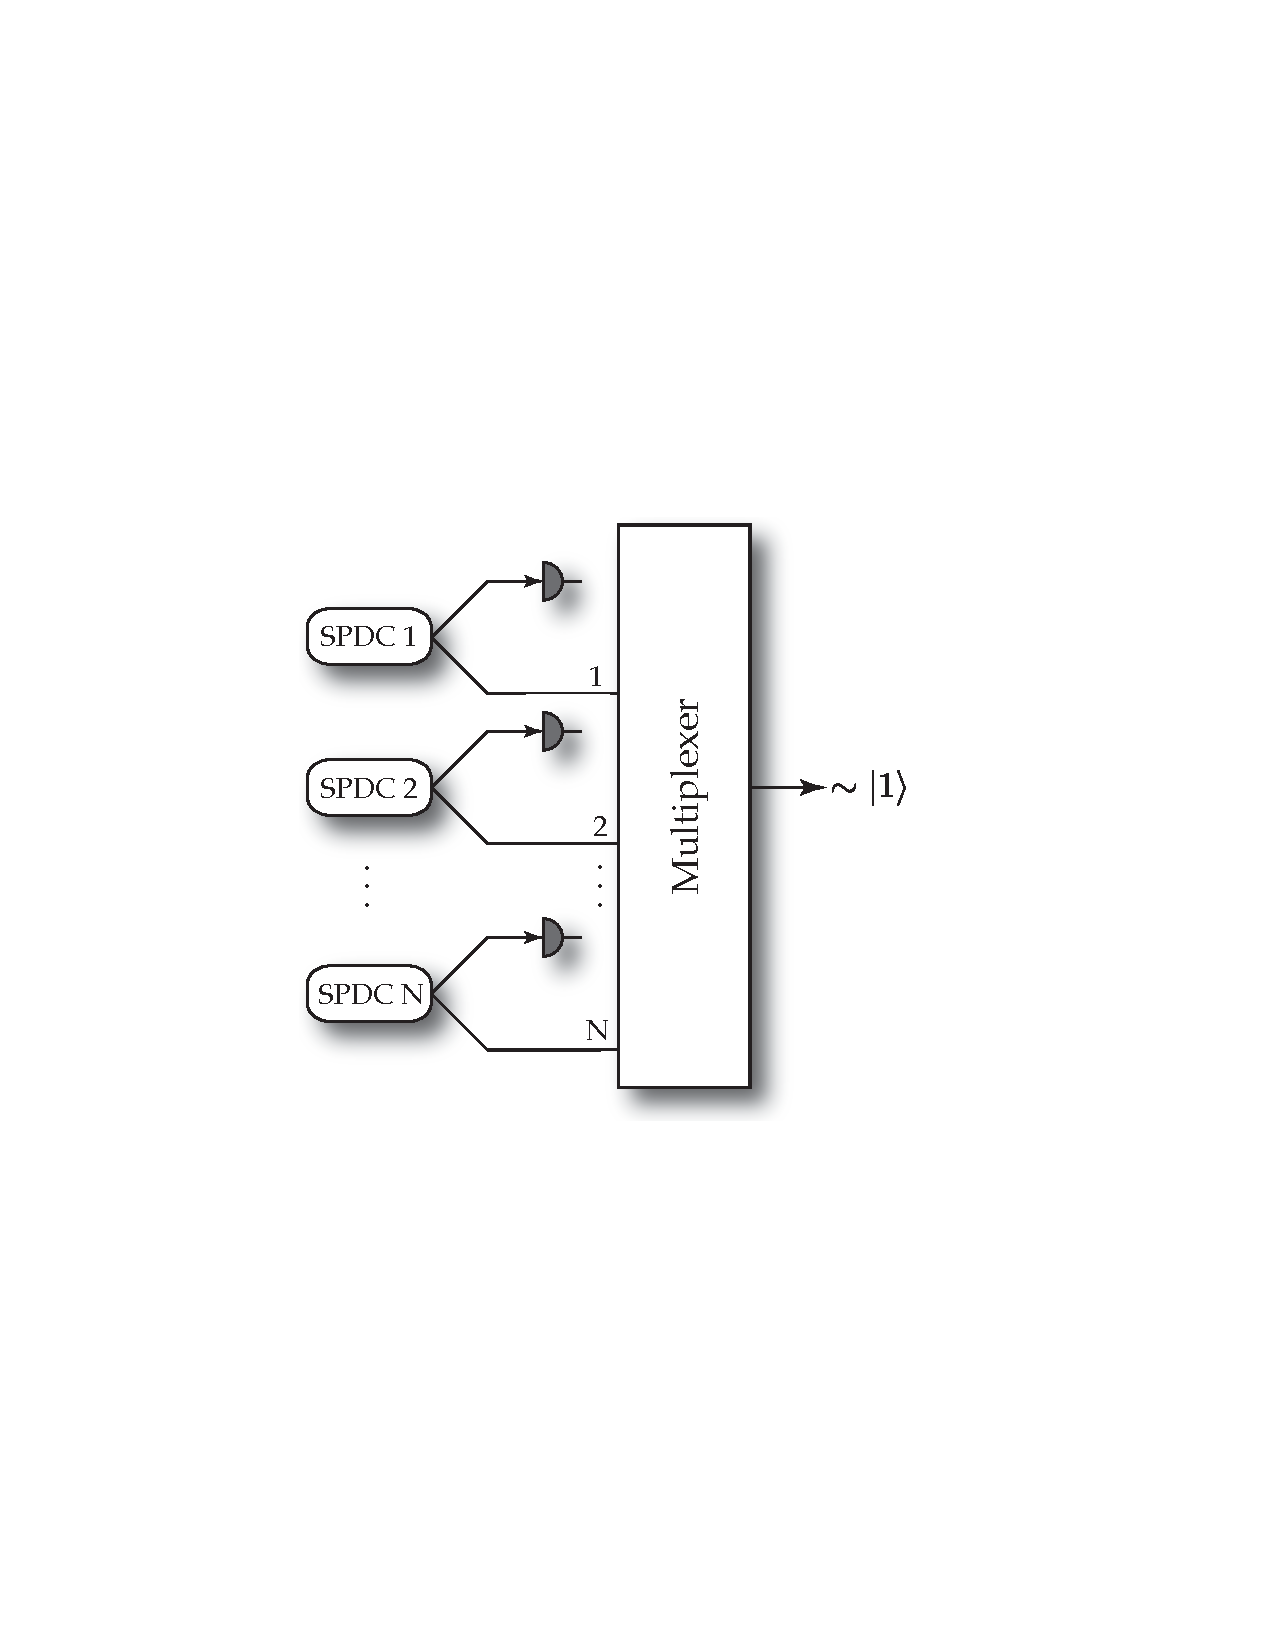
\includegraphics[width=0.75\columnwidth]{SPDC_multiplexing_arch}\index{Multiplexed single-photon sources}
\caption{Quasi-deterministic single photon state preparation using $N$-fold multiplexing of heralded SPDC sources (or any other non-deterministic, but heralded source). All $N$ SPDC sources are triggered simultaneously. The heralding detectors feedforward to the multiplexer, which routes a successfully heralded single photon state (if there is one) to the output mode. With a sufficiently large bank of sources in parallel, the probability of successfully preparing a single photon state approaches unity.} \label{fig:SPDC_multiplexing_arch}
\end{figure}

The success probability of the multiplexed source exponentially asymptotes to unity as the number of in-parallel sources increases,
\begin{align} \label{eq:SPDC_multiplex}
P_\text{success} = 1 - (1-P_\text{prep})^N,
\end{align}
where there are $N$ sources in parallel. This relationship is shown in Fig.~\ref{fig:SPDC_multiplexing_plot} for sources with varying heralding probabilities. This principle could also obviously be applied to any other type of non-deterministic, but heralded source.

\begin{figure}[!htb]
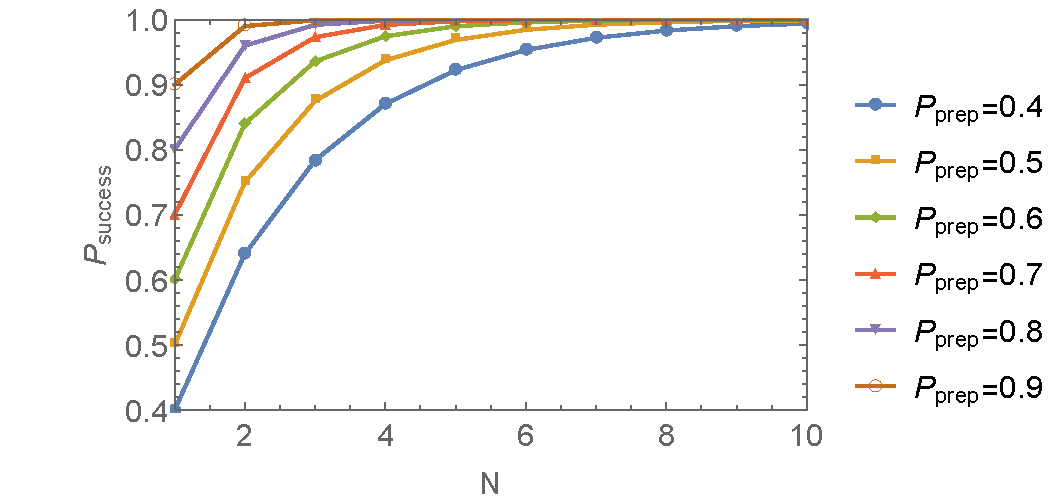
\includegraphics[width=\columnwidth]{SPDC_multiplexing_plot}
\caption{Single-photon state preparation probability, $P_\text{success}$, using $N$-fold multiplexing, where the individual heralded sources have heralding probability $P_\text{prep}$. $P_\text{success}$ always exponentially asymptotes to unity with increasing $N$, for any \mbox{$P_\text{prep}>0$}.} \label{fig:SPDC_multiplexing_plot}
\end{figure}

The multiplexing approach needn't be restricted to the spatial domain, but could also be equivalently implemented in the temporal domain \cite{bib:RohdeLoopMulti15, mosley, othersSeePaper}, as shown in Fig.~\ref{fig:SPDC_time_multiplexing}.

\begin{figure}[!htb]
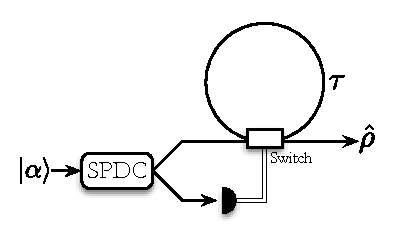
\includegraphics[width=0.75\columnwidth]{SPDC_time_multiplexing}
\caption{Multiplexed single-photon state preparation in the temporal domain. An SPDC source operating at high repetition rate, with time-bin separation $\tau$, enters a fibre-loop with an in/out coupling switch classically controlled by the heralding outcomes. The fibre-loop acts as a quantum memory, keeping the most recent successfully heralded time-bin in memory until the procedure terminates. The output is a pulse-train where the last time-bin closely approximates a single-photon.} \label{fig:SPDC_time_multiplexing}
\end{figure}

Of course, operating a large bank of sources in parallel, along with the associated multiplexing, which requires nanosecond-scale fast-feedforward, is experimentally costly (both in physical size, complexity and dollars), making outsourcing of this technology potentially highly desirable.

This description is purely in the photon-number basis. However, as discussed in Sec.~\ref{sec:spatio_temporal}, photons also have spatio-temporal characteristics. This strongly affects state preparation when using heralded SPDC, particularly state purity, and much effort has been invested into engineering the spectral structure of SPDC states so as to maximise purity and indistinguishability \cite{bib:Aichele02, bib:Branning00}.

SPDC is relatively cheap, and widely used, but nonetheless might be out of reach for many end-users, particularly when the previously discussed multiplexing techniques are employed to boost heralding efficiencies. It is quickly being superseded by superior technologies in cutting-edge labs, such as quantum dot sources, which have deterministic, push-button potential \cite{bib:Santori01, bib:Kiraz04}. Techniques based on cavity quantum electrodynamics (QED) \cite{bib:Brattke01} and molecular fluorescence \cite{bib:Brunel99} have also been demonstrated. However, such sources are very much in their developmental stages, and relatively expensive.

Generally speaking, a push-button photon source could be constructed from any two-level system, comprising a ground state, $\ket{g}$, and an excited state, $\ket{e}$, with short lifetime, whereby relaxation via the \mbox{$\ket{e}\to\ket{g}$} transition emits a photon. Then, pumping the system to excite it to the $\ket{e}$ state, and waiting for spontaneous decay yields a single photon.

%
% NOON States
%

\subsubsection{NOON states} \label{sec:NOON} \index{NOON state preparation}

So-called NOON states, path-number entangled two-mode states of the form,
\begin{align}
\ket\psi_\text{NOON} = \frac{1}{\sqrt{2}}(\ket{N,0}+\ket{0,N}),
\end{align}
may be exploited to perform Heisenberg-limited quantum metrology\index{Quantum metrology} (Sec.~\ref{sec:metrology}), allowing extremely precise phase measurement with large photon-number $N$ \cite{bib:Dowling08}. 

The extreme sensitivity of NOON states owes to the $N$-fold enhancement in phase-dependence associated with the $N$-photon component of the superposition. Specifically, if a phase $\phi$ is present in only the second mode, the state evolves to,
\begin{align}
e^{i\phi\hat{n}} \ket\psi_\text{NOON} = \frac{1}{\sqrt{2}}(\ket{N,0}+e^{i\phi N}\ket{0,N}),
\end{align}
where \mbox{$\hat{n}=\hat{a}^\dag\hat{a}$} is the photon-number operator associated with the second mode\index{Photon-number operator}. The phase enhancement arises because \mbox{$\hat{n}\ket{N}=N\ket{N}$}. Then, a simple interferometric procedure is able to extract this enhanced phase-dependence as an observable.

However, these states are notoriously difficult and technologically challenging to prepare, and can only be prepared non-deterministically using linear optics \cite{bib:Cable07}. If a remote server had the capacity to prepare such states, they would be in high demand across the globe. Hindering this, NOON states are very fragile creatures. First, they exhibit exponentially increased susceptibility to loss -- loss of just a single photon completely decoheres the state, rendering it useless for metrological purposes. Second, the large photon-number, $N$, amplifies unwanted dephasing by a factor of $N$, as discussed in Sec.~\ref{sec:dephasing_error}. These considerations can be readily accommodated for in the QTCP protocol by tracking dephasing and loss metrics of the packets encapsulating the NOON states.

\comment{Talk more about how to make them}

%
% Cluster States
%

\subsubsection{Cluster states} \index{Cluster state preparation}

In addition to the simple single- or two-mode states discussed above, an entire universal quantum computation can be performed using the `cluster state' measurement-based model for quantum computation (explained in detail in Sec.~\ref{sec:CSQC}). Here state preparation can not only be outsourced, but distributed, with different hosts preparing different parts of the state, which are then `stitched together'.

The beauty of this type of state is that there is a natural separation between state preparation and computation, with the preparation stage being far more technologically challenging than the computation stage. Thus, Alice might ask better-resourced Bob to prepare a cluster state and send it to her, at which point she implements the computation herself using simple single-qubit measurement operations.

%
% Greenberger-Horne-Zeilinger States
%

\subsubsection{Greenberger-Horne-Zeilinger states} \index{Greenberger-Horne-Zeilinger (GHZ) state preparation}

Another class of states is Greenberger-Horne-Zeilinger (GHZ) states \cite{bib:GHZ89}, which are maximally-entangled states across an arbitrary number of qubits, $n$, of the form,
\begin{align}
\ket\psi_\text{GHZ} = \frac{1}{\sqrt{2}}(\ket{0}^{\otimes n} + \ket{1}^{\otimes n}).
\end{align}

GHZ states are useful for various quantum information processing applications, including quantum anonymous broadcasting (Sec.~\ref{sec:anon_broad}). These states are particularly susceptible to loss, since the loss of a single qubit completely decoheres the state into a perfect mixture of the \mbox{$\ket{0}^{\otimes (n-1)}$} and \mbox{$\ket{1}^{\otimes (n-1)}$} states, with complete loss of entanglement and coherence,
\begin{align}
\hat\rho_\text{GHZ}^\text{loss} &= \text{tr}_1(\ket\psi_\text{GHZ}\bra\psi_\text{GHZ})\nonumber \\
&= \frac{1}{2}(\ket{0}^{\otimes (n-1)}\bra{0}^{\otimes (n-1)}+\ket{1}^{\otimes (n-1)}\bra{1}^{\otimes (n-1)}).
\end{align}

%
% Bell States
%

\subsubsection{Bell states} \label{sec:bell_state_res} \index{Bell state preparation}

Bell states, also known as Einstein-Podolsky-Rosen (EPR) pairs\index{Einstein-Podolsky-Rosen (EPR) pairs} \cite{bib:EPR35}, which are maximally-entangled two-qubit states, are particularly useful for many applications, including quantum teleportation (Sec.~\ref{sec:teleport}), cluster state preparation (Sec.~\ref{sec:CSQC}), and entanglement swapping (Sec.~\ref{sec:swapping}). Bell states are the special case of two-qubit cluster states, or equivalently, two-qubit GHZ states. They may be directly prepared as the two-mode output from a type-II\footnote{In type-II SPDC the photon-pair is polarisation-entangled, directly preparing a Bell-pair in the polarisation basis. In type-I SPDC both photons have the same polarisation, yielding only photon-number correlation, but no polarisation entanglement.} SPDC source, or using non-deterministic linear optics from single-photon sources.

There are four Bell states, defined as, 
\begin{align} \label{eq:bell_basis}
\ket{\Phi^{\pm}} &= \frac{1}{\sqrt{2}} (\ket{0}_A\ket{0}_B \pm \ket{1}_A\ket{1}_B), \nonumber \\
\ket{\Psi^{\pm}} &= \frac{1}{\sqrt{2}} (\ket{0}_A\ket{1}_B \pm \ket{1}_A\ket{0}_B),
\end{align}
which are locally equivalent to one another via the application of Pauli operators, and may therefore be transformed to one another without classical or quantum communication between the two parties. Specifically,
\begin{align}
\ket{\Phi^+} = \hat{Z}\ket{\Phi^-} = \hat{X}\ket{\Psi^+} = \hat{X}\hat{Z}\ket{\Psi^-},
\end{align}
where $\hat{X}$ and $\hat{Z}$ could apply to either qubit, up to global phase.

In Sec.~\ref{sec:ent_ultimate} we present the case that these states are so useful on their own that one might be justified in building entire quantum networks based purely upon the distribution of Bell-pairs. This is the basis for \textit{quantum repeater networks}, which will be discussed in Sec.~\ref{sec:rep_net}.

%
% Cat States
%

\subsubsection{Cat states} \index{Cat state preparation}

Cat states (Sec.~\ref{sec:cat_enc}) -- superpositions of coherent states -- are extremely difficult to prepare, most easily via non-linear processes. However, they are very useful for optical quantum computation and for the study of macroscopic quantum systems, when using large coherent amplitudes. Because of the difficulty of their preparation, the ability to outsource it would be very valuable.

However, it must be cautioned that cat states decohere very readily, since their well-defined parity implies decoherence upon loss of just a single photon. This makes QoS considerations particularly pertinent.

%
% Squeezed States
%

\subsubsection{Squeezed states} \label{sec:squeezed} \index{Squeezed state preparation}

Of particular interest to metrology\index{Quantum metrology} in particular, are squeezed states, states which have been longitudinally distorted in phase-space. In the metrological context, squeezed states enable sub-shotnoise limited metrology \cite{???}, thereby outperforming any classical protocol, using, for example, coherent states.

Mathematically, squeezing is represented using the squeezing operator,
\begin{align}
\hat{S}(\xi) = \text{exp}\left[ \frac{1}{2}(\xi^*\hat{a}^2 - \xi{\hat{a}^{\dag 2}})\right],
\end{align}
where $\hat{a}$ is the photonic creation operator, and $\xi$ is the squeezing parameter. Experimentally, such states are prepared using non-linear crystals. It is intuitively obvious that linear optics alone cannot prepare such states, owing to the non-linear terms in the squeezing operator, which do not preserve photon-number, and therefore cannot be passive.

Of particular interest are squeezed coherent states, $\hat{S}(\xi) \ket{\alpha}$, which are minimum uncertainty states, saturating the Heisenberg uncertainty relation. A special case of this is squeezed vacuum states, $\hat{S}(\xi) \ket{0}$, which are even-parity states (i.e containing strictly even photon-number terms). This implies that, like cat states, they are very vulnerable to decoherence for the same reason.

%
% More Exotic States of Light
%

\subsubsection{More exotic states of light}

As discussed in Sec.~\ref{sec:exotic}, many other far more elaborate states are very difficult to prepare, and it would be highly desirable if they could be obtained/purchased over a quantum network. This includes certain CV states, which have utility in alternate models for quantum computing \cite{bib:Menicucci06, Ralph, Lund}.

\comment{To do!}

\comment{Add hyperlinks to other relevant sections}

%
% Matter Qubits
%

\subsubsection{Matter qubits} \index{Matter qubits}

In addition to preparing optical states, they can be used to mediate the preparation of systems comprising matter qubits, using which-path erasure techniques (Sec.~\ref{sec:hybrid} \& Fig.~\ref{fig:barrett_kok}) or light-matter interactions (Sec.~\ref{sec:opt_inter} \& Fig.~\ref{fig:opt_int}). These techniques are very versatile, and apply to many different matter qubit systems, such as two-level atoms, nitrogen-vacancy centres, quantum dots, and atomic ensembles.

This is useful when matter-based architectures are more scalable or technologically simpler than all-optical architectures (Sec.~\ref{sec:KLM_univ}), and particularly for quantum memory (Sec.~\ref{sec:memory}), when using matter qubits with long lifetimes.

%
% Measurement
%

\subsection{Measurement} \index{Measurement}

As a last (and possibility also intermediate) step in any quantum protocol is the measurement of quantum states. State measurement is, in the most general context, essentially state preparation in reverse, and brings with it many of the same challenges.

Different detection schemes bring with them their own (potentially substantial) costs and technological challenges. State of the art micropillar photo-detectors \cite{???}, at the time of writing, cost on the order of \$100k's, and require a sophisticated laboratory setup. Clearly this type of infrastructure is inaccessible to many players, and borrowing or licensing access to such equipment over a quantum network would pave the way for broader accessibility to state of the art technology.

Each type of state being measured, in combination with the nature of the detection scheme, brings with it their own limitations. For example, number-resolved photo-detectors exhibit dead-time, are too slow to enable fast-feedforward, have spectral filtering characteristics, and mode-matching requirements. \comment{Is this right?}

These represent significant technological challenges, which are costly to overcome, necessitating outsourcing over the quantum internet to become economically viable on a large scale. However, the QTCP protocol is able to accommodate error metrics and attributes covering all the above error models, enabling reliable, predictable QoS for outsourced quantum measurement.

With the ability to perform measurements over a complete basis for the respective system, QST, and consequently QPT (Sec.~\ref{sec:QPT}), can also be outsourced, as both these protocols are built entirely upon determining measurement expectation values in some known basis.

%
% Photo-detection
%

\subsubsection{Photo-detection} \label{sec:photo_detection} \index{Photo-detection}

Perhaps the most useful, and ubiquitous, type of optical state measurement is photo-detection \cite{RohdePDReview}, where we would like to count photon-number. Broadly, there are two main classes of photo-detectors -- \textit{number-resolved} and \textit{non-number-resolved} (or `bucket' detectors). These behave exactly as the names suggest, with the former typically being more expensive and technologically demanding than the latter.

The most common form of photo-detection is using avalanche photo-diodes (APDs)\index{Avalanche photo-diodes (APDs)}, which are cheap but non-number-resolving. Here a single photon excites an electron into the conduction band at a semiconductor junction, enabling a detectable current flow.

More recently, superconducting detectors\index{Superconducting photo-detectors} have been adopted, as they have the potential for number-resolution. Here a superconductor is kept just below its critical temperature, and the absorption of a photon is enough to heat the superconductor above the critical temperature, creating a detectable change in resistance across the superconductor. This is shown in Fig.~\ref{fig:super_det}. Despite their superior performance, however, superconducting detectors are very expensive (for obvious reasons) and only accessible to well-resourced labs.

\begin{figure}[!htb]
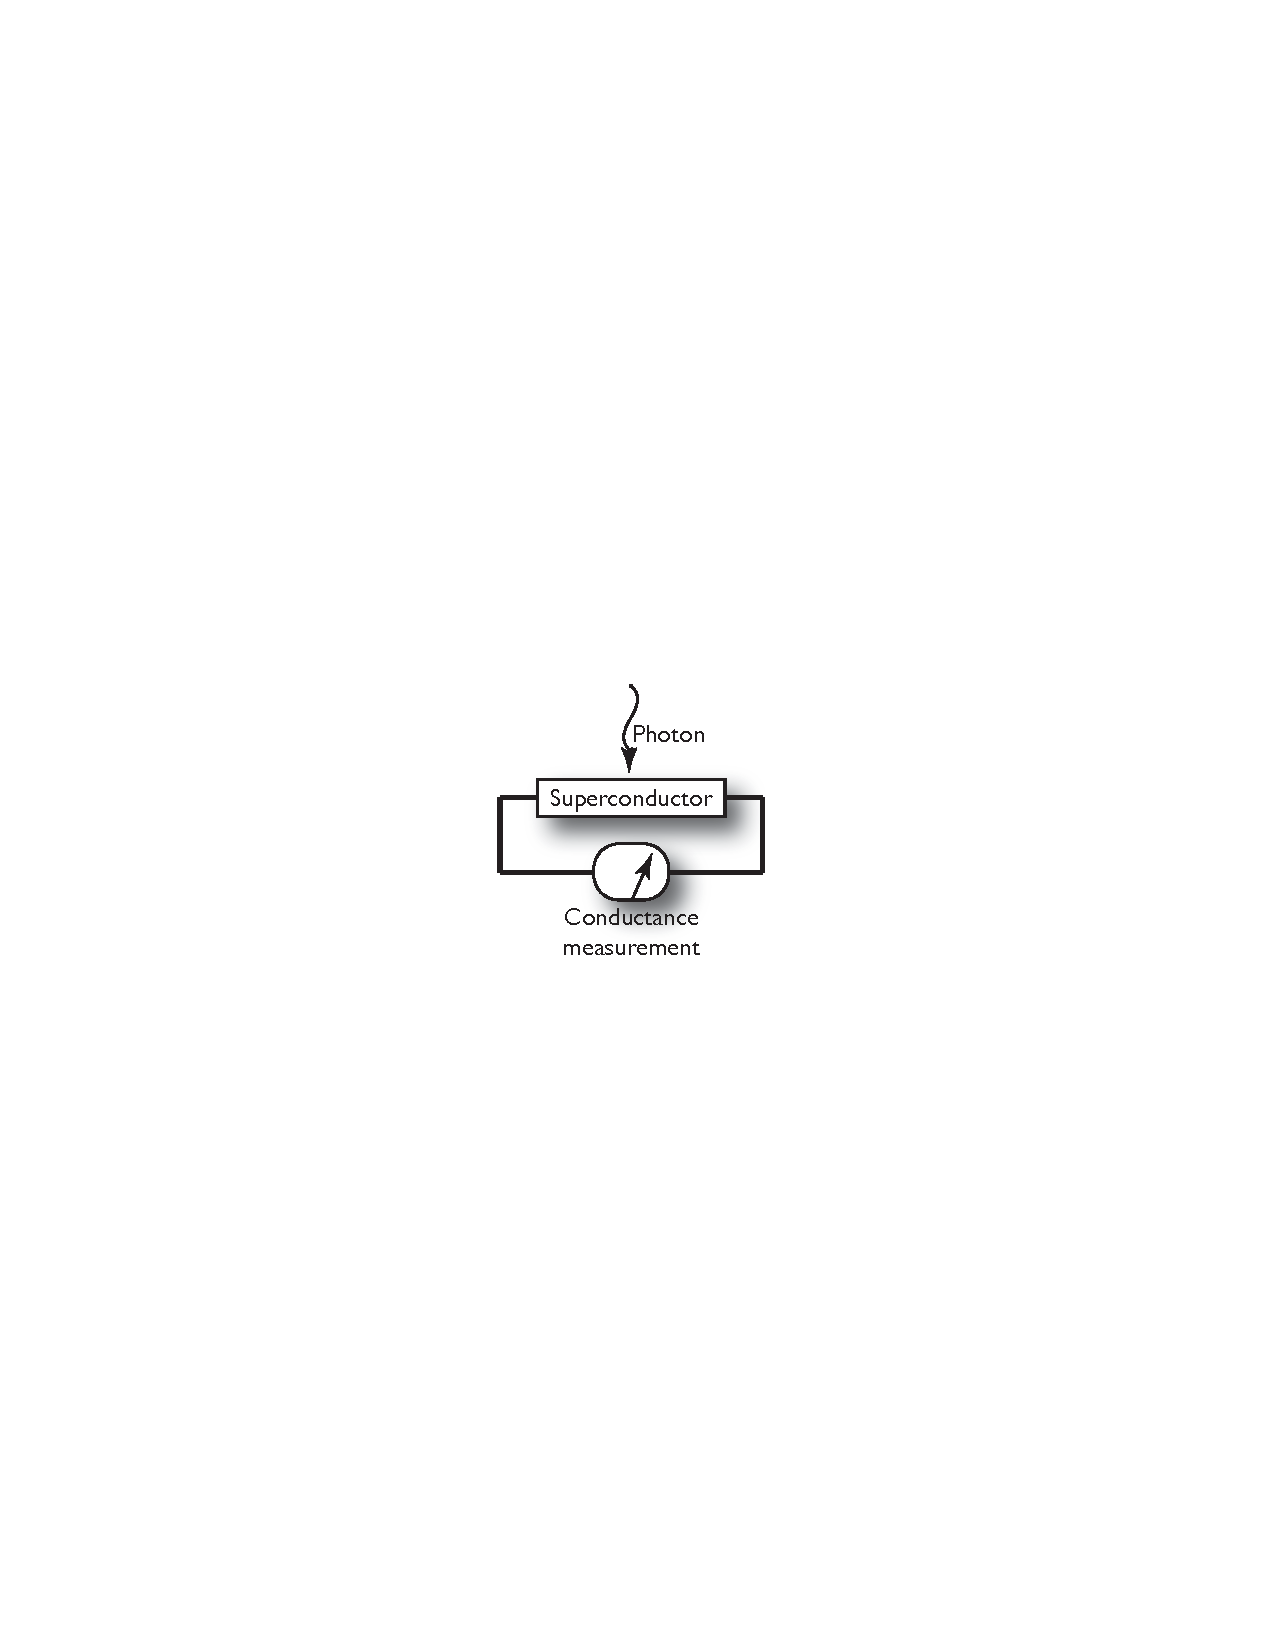
\includegraphics[width=0.5\columnwidth]{superconducting_detector}
\caption{A superconducting photo-detector. A superconductor is held at just below its critical temperature. The absorption of a photon is sufficient to heat it above the critical temperature, yielding a detectable change in conductance across the device.} \label{fig:super_det}
\end{figure}

The key parameter of interest in a photo-detector, in addition to whether or not it is number-resolving, is its efficiency\index{Detector efficiency}, $\eta$ -- the probability that a given incident photon will trigger the detector. For most applications, the goal is to maximise $\eta$. As one might expect, there is a direct tradeoff between $\eta$ and cost, with very high-efficiency detectors often economically out of reach for many experimentalists. Also of interest is the `dark-count' rate -- the rate at which the detector falsely clicks in the absence of photons. However, this is often ignored as modern detectors typically exhibit very low dark-count-rates.

Mathematically, the measurement operators for number-resolved detection are,
\begin{align}\index{Number-resolved photo-detection}
\hat\Pi_n = \eta^{n} \sum_{m=n}^\infty \binom{m}{n} (1-\eta)^{m-n} \ket{m}\bra{m},
\end{align}
for measurement outcome $n$, in the photon-number basis. And for non-number-resolved detection,
\begin{align}\index{Non-number-resolved photo-detection}
&\hat\Pi_0 = \sum_{m=0}^\infty (1-\eta)^{m} \ket{m}\bra{m}, \nonumber \\
&\hat\Pi_{>0} = \mathbb{\hat{I}} - \hat\Pi_0.
\end{align}
Thus, inefficiency results in projection onto the wrong photon-number, making measurement outcomes incorrect.

Number-resolved detectors are the more challenging ones to experimentally realise. However, using multiplexing techniques\index{Multiplexed photo-detection}, non-number-resolved detectors can be used to closely approximate number-resolution \cite{bib:Fitch03, bib:Banaszek03, bib:Achilles04, bib:RohdeCompDet07}, at the expense of an (efficient) overhead in the complexity of the experiment, which comes at a cost. Specifically, there is a direct tradeoff between the confidence in photon-number outcomes, and experimental overhead. The idea behind this is simple. We spread out an $n$-photon state evenly across a large number of modes, $m$, and detect each one independently using a non-number-resolved photo-detector. If \mbox{$m\gg n$}, it is unlikely that more than a single photon will reach any given detector. Thus, by summing the total number of clicks across all detectors, we closely approximate the true photon-number. This multiplexing can be performed in the spatial- or temporal-domains, shown in Fig.~\ref{fig:det_mult}, and has been a widely employed technique in laboratories without access to expensive number-resolved detectors.

\begin{figure}[!htb]
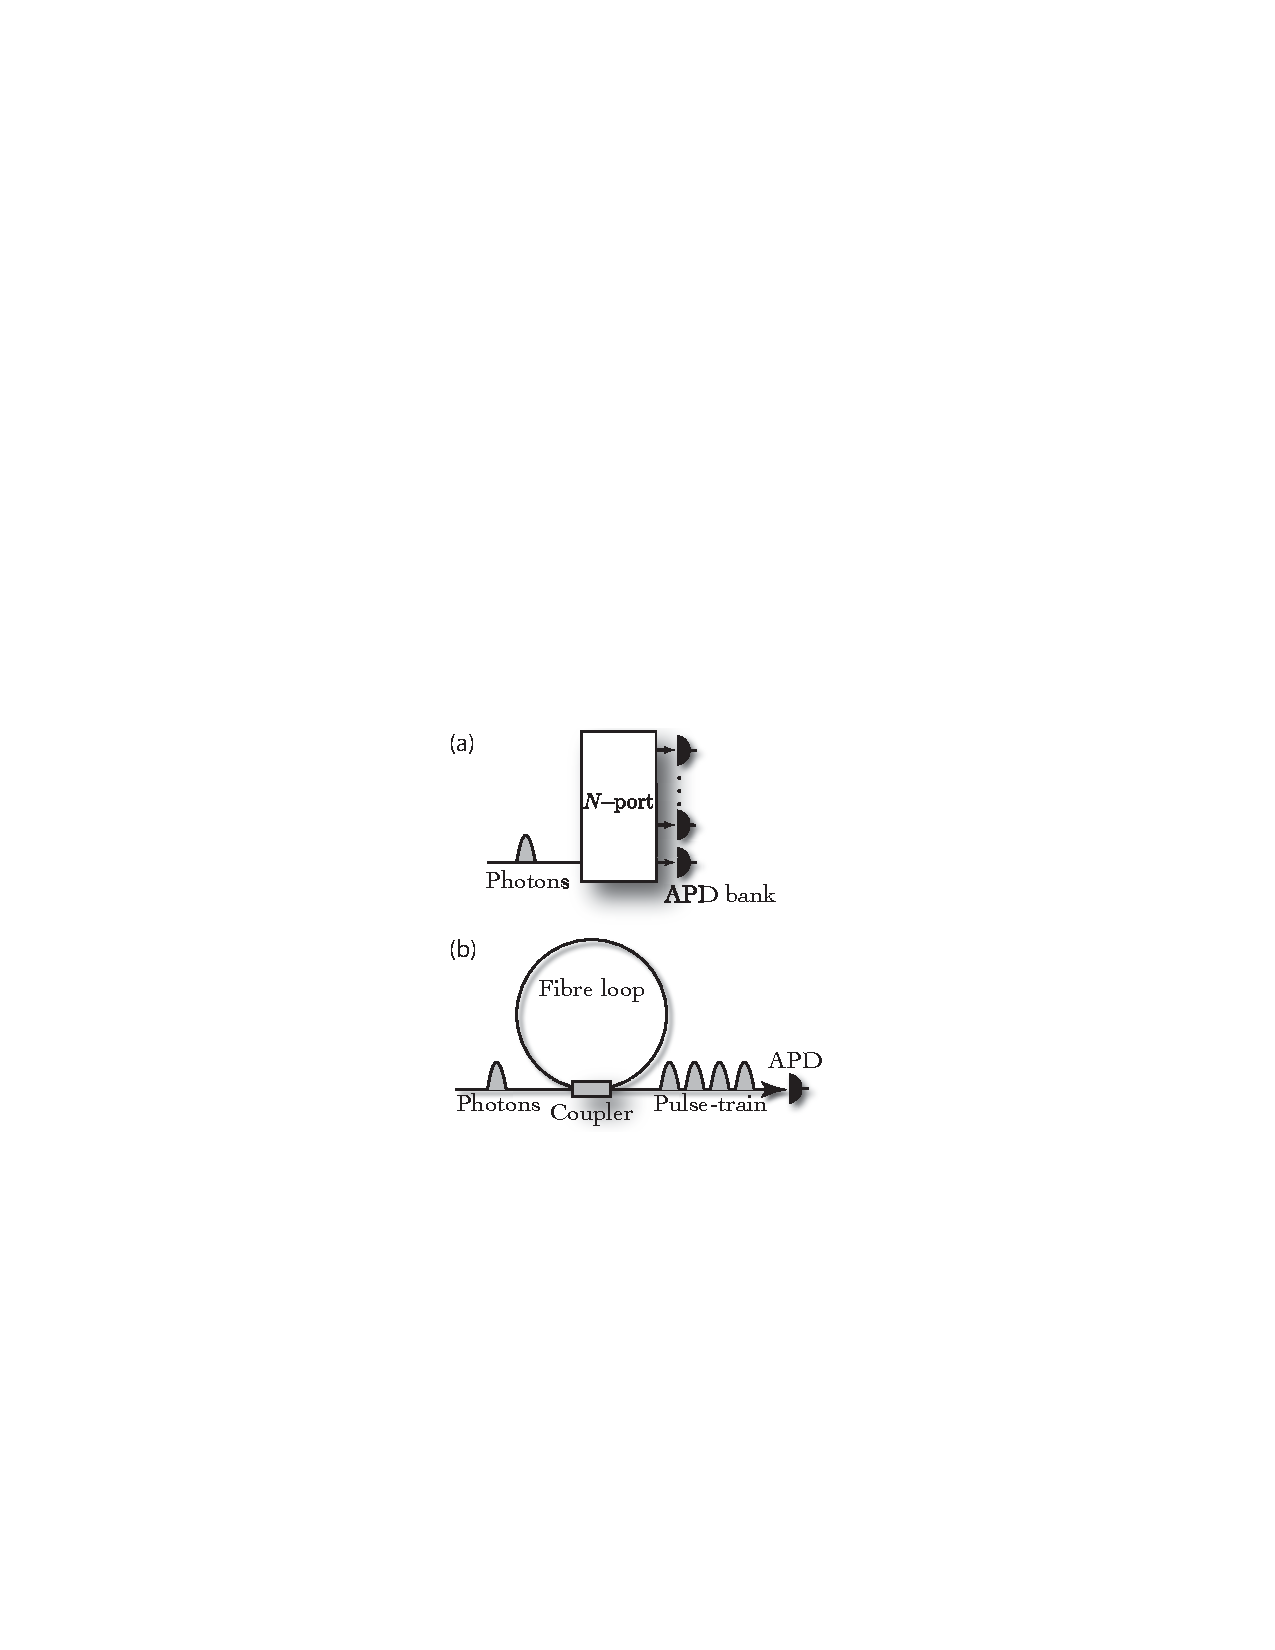
\includegraphics[width=0.7\columnwidth]{detector_multiplexing}
\caption{Multiplexed number-resolved photo-detection using non-number-resolved photo-detectors. The principle is to spread out a multi-photon state across a large number of modes, sufficiently large that it is unlikely that more than one photon will be present in any given mode. Then, the sum of the number of clicks at each mode closely approximates the incident photon-number. (a) In the spatial domain. (b) In the temporal domain.} \label{fig:det_mult}
\end{figure}

In addition to their operation in the photon-number basis, photo-detectors exhibit spatio-temporal characteristics, which affect their operation in quantum information processing protocols \cite{RohdePDReview}. For example, imperfect spectral response can undermine photonic interference, affecting which-path erasure protocols, such as Bell state projection (Sec.~\ref{sec:bell_proj}). However, in many cases this can be improved upon using spectral filtering or time-gating techniques, also at the expense of experimental complexity and resource overhead.

Furthermore, photo-detectors are subject to `dead-time'\index{Dead-time}, which renders them inactive for a finite recovery period following a detection event. This is of especial importance in time-bin-encoded schemes (Sec.~\ref{sec:time_bin}), where detectors must resolve photons over very short timescales on the order of nanoseconds.

Finally, photo-detectors of all types are inevitably subject to `dark-counts'\index{Dark-counts}, whereby thermal noise, either within the detector or coupled from the noisy environment, triggers non-existent detection events. The distribution follows exactly that of the thermal state photon-number distribution (Sec.~\ref{sec:thermal_states}). Thus, the probability of $n$ dark-counts occurring is,
\begin{align} \index{Thermal distribution}
p_\text{dc}(n) = e^{-|\alpha|^2} \frac{|\alpha|^2}{n!},
\end{align}
where $\alpha$ is a parameterisation of the temperature of the environmental noise. Fortunately, modern detector technology is able to keep dark-count rates very low, making this far less of an issue than the aforementioned ones, loss being the dominant.

%
% Homodyning
%

\subsubsection{Homodyning} \label{sec:homodyne} \index{Homodyning}

A homodyne detector interferes a state with a coherent state on a beamsplitter, which acts as a phase-reference, before photo-detecting both output modes and taking the difference in the photon count-rates (Fig.~\ref{fig:homodyne}). By sweeping through the amplitude and phase of the reference beam, we are able to directly sample points in phase-space, allowing the Wigner function -- which is isomorphic to the density operator -- of an unknown state to be fully reconstructed. This measurement technique is typically applied to CV states rather than photon-number states. While conceptually straightforward, preparing the reference beam requires a coherent source, which can become costly (Sec.~\ref{sec:coherent_states}).

\begin{figure}[!htb]
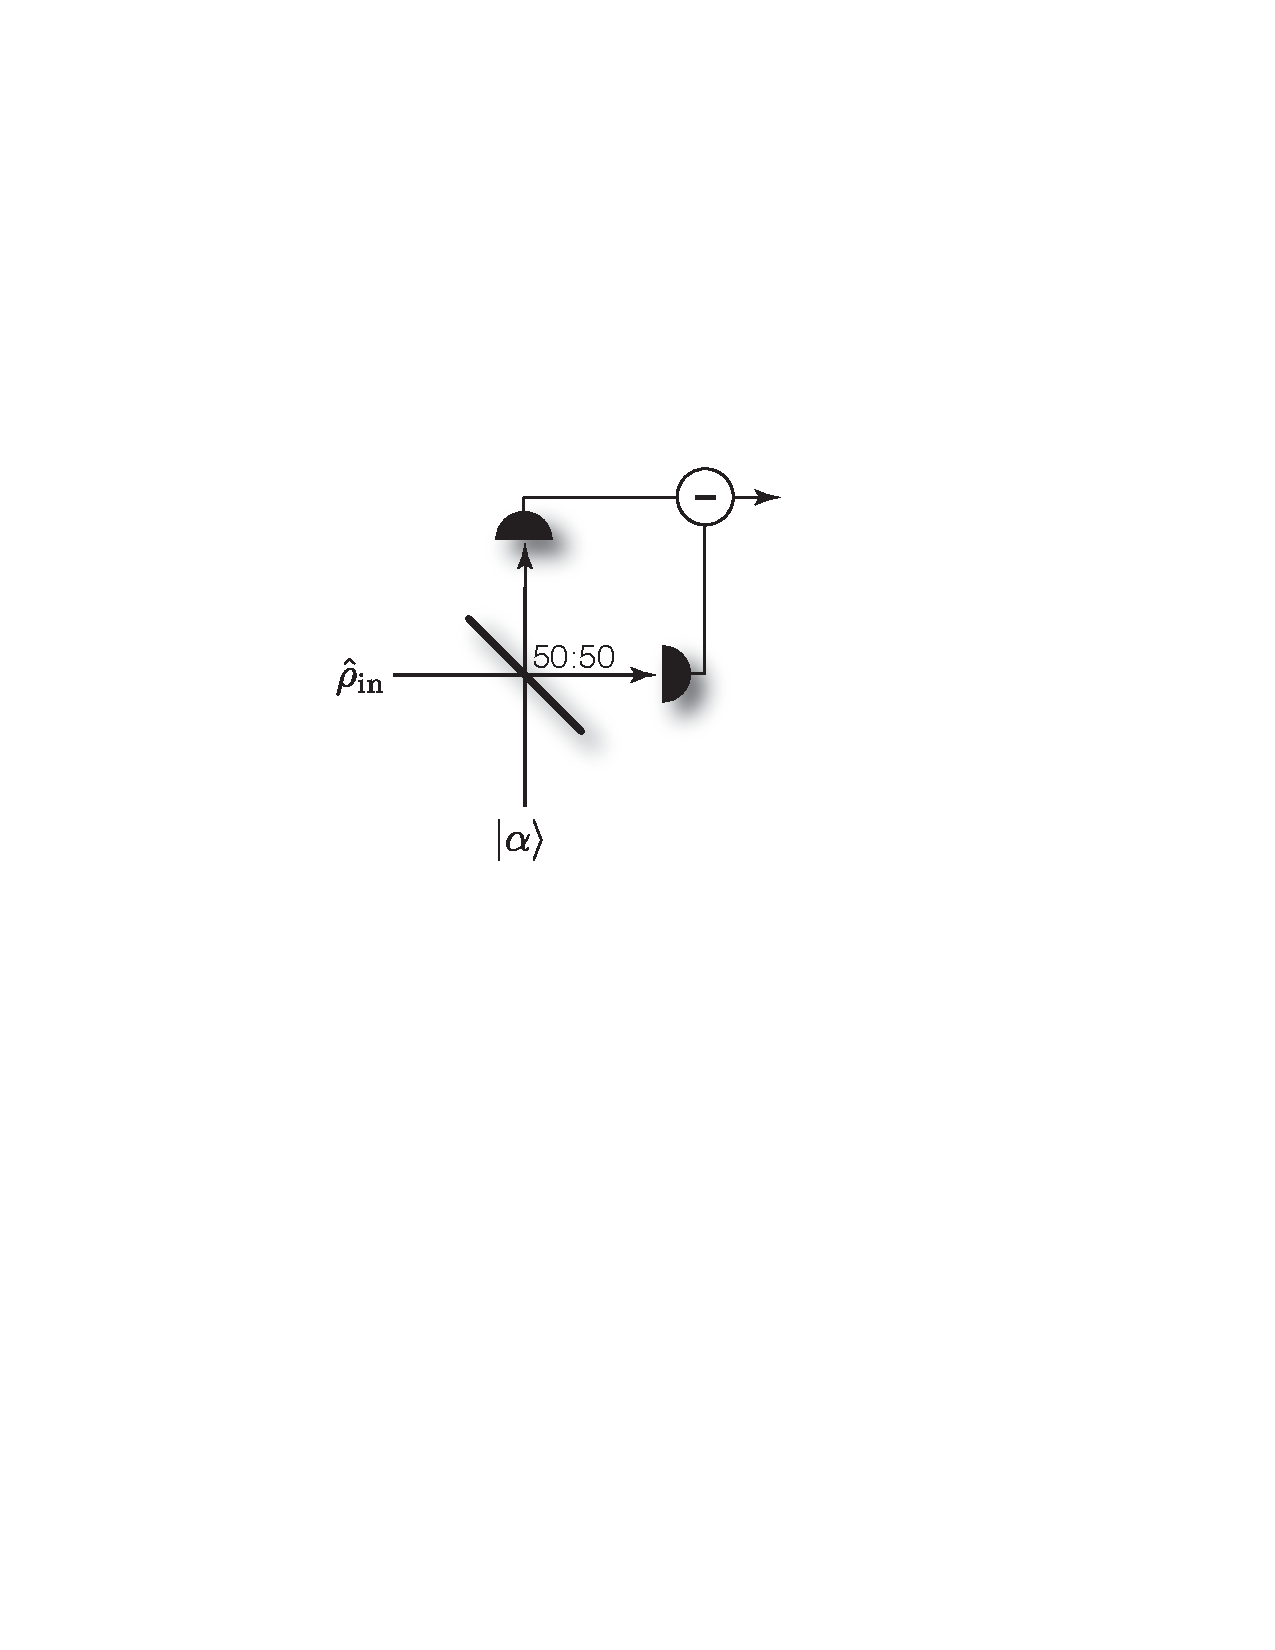
\includegraphics[width=0.6\columnwidth]{homodyne}
\caption{Homodyne detection of an unknown optical state $\hat\rho_\text{in}$, by mixing it with a reference coherent state $\ket\alpha$ on a 50:50 beamsplitter, and taking the difference in the photo-detection rates at the output modes. By sweeping through the phase and amplitude of $\ket\alpha$, we can directly sample the Wigner function of $\hat\rho_\text{in}$, allowing its full reconstruction.} \label{fig:homodyne}
\end{figure}


%
% Bell State & Parity Measurements
%

\subsubsection{Bell state \& parity measurements} \label{sec:bell_proj} \index{Bell measurements}

For the purposes of which-path erasure, essential for optical cluster state (Sec.~\ref{sec:CSQC}) preparation and quantum teleportation (Sec.~\ref{sec:teleport}), Bell state measurements [i.e projections onto the Bell basis given in Eq.~(\ref{eq:bell_basis})] are important.

To realise this, there are two primary options. The first is to use a CNOT gate, for example an LOQC gate (Sec.~\ref{sec:KLM_univ}). The second is to perform a \textit{partial} Bell state projection using a polarising beamsplitter (PBS) -- a beamsplitter which completely transmits vertical polarisation, and completely reflects horizontal polarisation \cite{bib:BraunsteinMann95}.

In the Heisenberg picture, the transformation of the photonic creation operators implemented by a PBS is,
\begin{align}\index{Polarising beamsplitters}
\hat{h}_1^\dag &\to \hat{h}_2^\dag, \nonumber \\
\hat{h}_2^\dag &\to \hat{h}_1^\dag, \nonumber \\
\hat{v}_1^\dag &\to \hat{v}_1^\dag, \nonumber \\
\hat{v}_2^\dag &\to \hat{v}_2^\dag,
\end{align}
where $\hat{h}_i^\dag$ ($\hat{v}_i^\dag$) are the horizontal (vertical) creation operators for the $i$th mode. The measurement projectors implemented by the PBS, when both modes are measured in the diagonal ($+/-$) basis, are then,
\begin{align}
	\hat\Pi_\text{Bell}^+ &= \ket{H,H}\bra{H,H}+\ket{V,V}\bra{V,V}, \nonumber \\
	\hat\Pi_\text{Bell}^- &= \ket{H,H}\bra{H,H}-\ket{V,V}\bra{V,V}, \nonumber \\
	\hat\Pi_
	\text{HV} &= \ket{H,V}\bra{H,V}, \nonumber \\
\hat\Pi_
	\text{VH} &= \ket{V,H}\bra{V,H},
\end{align}
where the former two represent successful projection onto the Bell basis, and the latter two represent failures, effectively measuring both modes in the $H/V$ basis. This approach is described in Fig.~\ref{fig:partial_bell}.

Technically, $\hat\Pi^\pm_\text{Bell}$ are not Bell measurements, but rather projections onto the even parity subspace. A true Bell projection would implement $\ket{\Phi^\pm}\bra{\Phi^\pm}$. However, in an optical context the two terms are often used interchangeably, since they exhibit effectively the same behaviour, given that the detection process is destructive.

Bell projections using CNOT gates can be implemented with arbitrarily high success probability in principle. However, in most scenarios of interest (such as cluster state preparation and entanglement purification) Bell projection using a PBS succeeds with probability of $1/2$, since a PBS is only able to uniquely distinguish two of the four Bell states. To its advantage, such `partial' Bell measurements only require high HOM visibility, avoiding the need for the interferometric stability inherent internally within LOQC CNOT gates.

\begin{figure}[!htb]
\includegraphics[width=0.75\columnwidth]{partial_bell}
\caption{Partial Bell state projection using a polarising beamsplitter (PBS). The PBS completely transmits horizontally polarised light, whilst completely reflecting vertically polarised light. Shown are the four possible two-photon input states, and the respective trajectories followed by the photons. To complete the partial Bell projection we measure the output modes in the diagonal basis, \mbox{$\ket{\pm} = \frac{1}{\sqrt{2}}(\ket{H}\pm\ket{V})$}, such that horizontally and vertically polarised photons cannot be distinguished. If the input state was $\ket{H,H}$ or $\ket{V,V}$, we would measure one photon in each output mode (both transmitted or both reflected). Since the detectors cannot distinguish $\ket{H}$ from $\ket{V}$, this effectively projects us onto the coherent superposition of both possibilities (`which-path erasure'), implementing the measurement projector \mbox{$\hat\Pi_\text{Bell}^\pm = \ket{H,H}\bra{H,H}\pm\ket{V,V}\bra{V,V}$}. If, on the other hand, we measure two photons at one output mode, we know with certainty what the polarisations of both incident photons were and we probabilistically implement one of the projectors \mbox{$\hat\Pi_
\text{HV}=\ket{H,V}\bra{H,V}$} or \mbox{$\hat\Pi_
\text{VH}=\ket{V,H}\bra{V,H}$}, effectively performing polarisation-resolved detection upon both modes, which equates to a $\hat{Z}$ measurement on the logical qubits. The practical outcome of this is that, when using a PBS to prepare cluster states, with probability $1/2$ we are able to successfully fuse two smaller cluster states together into a larger one, and with probability $1/2$ we fail to do so, instead removing two qubits from the clusters.} \label{fig:partial_bell}
\end{figure}

While partial Bell state projection using a PBS is relatively straightforward, LOQC CNOT gates (which are very desirable owing to their near-determinism) are very technologically challenging, with drastic resource overheads, particularly for high success probability. Thus, outsourcing them to the cloud may be very economically efficient.

%
% Detector Banks
%

\subsubsection{Detector banks} \index{Detector banks}

In the case of an entire quantum computation, whether it be in the circuit model or cluster state model, many qubits may need to be measured independently, adding a direct multiplicative overhead in the required number of detectors. Furthermore, in protocols requiring fast-feedforward, the detectors may be required to have very fast time-response. These requirements can quickly become very challenging and expensive, further exaggerating the desirability of outsourcing the measurement stage.

%
% Matter Qubits
%

\subsubsection{Matter qubits} \index{Matter qubits}

Many non-optical systems can be indirectly measured by first entangling optical states with the matter qubits and then measuring the optical state. Because of the entanglement, projective measurement on the optical state teleports the measurement onto the matter qubit.

In Fig.~\ref{fig:barrett_kok} we illustrate a scheme for entangling two $\lambda$-configuration atoms using which-path erasure. Consider just one of these qubits in isolation. If a $\pi$-pulse is applied to the atom, the $\ket{\!\downarrow}$ state is excited to the $\ket{e}$ state, after which, upon relaxation, it emits a photon. Thus, upon measurement, the presence or absence of a photon directly indicates whether the qubit was in the $\ket{\!\uparrow}$ or $\ket{\!\downarrow}$ state.

The attractive feature of this is that although the matter qubit is stationary, its indirect measurement via optical coupling may be performed over arbitrary distances across the optical network, allowing the measurement stage to be outsourced. This includes entangling measurements, useful for, for example, cluster state preparation (Sec.~\ref{sec:CSQC}).

%
% Quantum non-demolition measurement (QND)
%

\subsubsection{Quantum non-demolition measurement (QND)}

\comment{To do!}

%
% Evolution
%

\subsection{Evolution}

The evolution of optical states represents an extremely broad category of quantum operations, including: passive linear optics; post-selected linear optics; non-linear optics; and, light-matter interactions. Clearly, the items in this list present technological challenges, inaccessible to many users.

The error models in the evolution of optical states are largely accounted for by those discussed in Sec.~\ref{sec:errors_in_nets}. 

%
% Linear Optics
%

\subsubsection{Linear optics} \label{sec:LO_ev_archs} \index{Linear optics evolution}

Linear optics networks implement unitary linear maps on the photonic creation operators, of the form,
\begin{align} \label{eq:LO_unitary_map}
\hat{U}\hat{a}_i^\dag \hat{U}^\dag \to \sum_{j=1}^m U_{i,j} \hat{a}^\dag_j,
\end{align}
where $\hat{a}^\dag_i$ is the photonic creation operator on the $i$th of the $m$ modes, and $U$ may be any $\text{SU}(m)$ matrix. It was shown by \cite{bib:Reck94} that arbitrary transformations of this form may be decomposed into $O(m^2)$ linear optical elements (beamsplitters and phase-shifters), enabling efficient construction of arbitrary linear transformations.\index{Linear optics decompositions} Furthermore, the algorithm for determining the decomposition of such transformations has polynomial classical runtime (i.e residing in \textbf{P}\index{\textbf{P} \& \textbf{BPP}}). Note that the original Reck \emph{et al.} decomposition is not unique, and various other topologies of optical elements also enable universality \cite{???}.

Each individual beamsplitter in such a decomposition is an arbitrary $\text{SU}(2)$ matrix acting on two photonic creation operators, $\hat{a}^\dag$ and $\hat{b}^\dag$,
\begin{align}\index{Beamsplitters}
\begin{pmatrix}
\hat{a}^\dag_\text{out} \\
\hat{b}^\dag_\text{out}
\end{pmatrix}=\begin{pmatrix}
U_{11} & U_{12} \\
U_{21} & U_{22}
\end{pmatrix}\begin{pmatrix}
\hat{a}^\dag_\text{in} \\
\hat{b}^\dag_\text{in}
\end{pmatrix}.
\end{align}
When operating in the polarisation basis, wave-plates\index{Wave-plates} enable the same transformation as beamsplitters do in dual-rail encoding. The phase-shifters implement the unitary operation,\index{Phase-shifters}
\begin{align}
\hat\Phi(\phi)=e^{-i\phi\hat{n}},
\end{align}
or equivalently in the Heisenberg picture,
\begin{align}
\hat{U}\hat{a}^\dag\hat{U}^\dag \to e^{-i\phi}\hat{a}^\dag,
\end{align}
for phase-shift $\phi$.

These linear optics evolutions are most commonly implemented using either:
\begin{itemize}
\item Bulk optics: where discrete optical elements are arranged on an optical table.\index{Bulk optics}
\item Time-bin architectures: where time-bin encoded qubits (Sec.~\ref{sec:time_bin}) evolve through delay lines and interfere at a single central optical component.\index{Time-bin encoding}\index{Fibre-loops}
\item Integrated waveguides: where all passive components are etched into a chip.\index{Waveguides}
\end{itemize}
These three main contenders are illustrated in Fig.~\ref{fig:LO_archs}, and described in more detail in Sec.~\ref{sec:LO_evolution}.

\begin{figure}[!htb]
\includegraphics[width=\columnwidth]{LO_archs}
\caption{The three primary approaches for implementing linear optics transformations. (a) Bulk optics\index{Bulk optics}, where each optical mode is spatially encoded, and the linear transformation is decomposed into a discrete array of beamsplitters and phase-shifters, an appropriate choice of which enables arbitrary linear optics transformations to be implemented. (b) Time-bin encoding\index{Time-bin encoding}\index{Fibre-loops}, where each optical mode is designated a distinct time-bin. Fibre-loops meeting at dynamically reconfigurable beamsplitters enable arbitrary linear transformations to be implemented. (c) Integrated wave-guide chips\index{Waveguides}, where evanescent coupling between neighbouring wave-guides within a chip facilitates interference between modes (graphic courtesy of Alberto Peruzzo \cite{bib:PeruzzoQW}).} \label{fig:LO_archs}
\end{figure}

%
% Non-Linear Optics
%

\subsubsection{Non-linear optics} \label{sec:non_lin_opt} \index{Non-linear optics}

Aside from the linear transformations described above, which are passive and photon-number-preserving, various active, non-linear interactions are also of interest to optical quantum information processing. The most prominent of these are primarily considered as transformations in phase-space (Sec.~\ref{sec:exotic}), using, for example, the Wigner function representation.

The most well-known non-linear transformation is the displacement operation, which translates the Wigner function by some arbitrary amplitude in phase-space, whilst preserving all other features of the phase-space representation. This is described by the unitary operator,\index{Displacement operator}
\begin{align}
\hat{D}(\alpha) = \text{exp}\left[\alpha\hat{a}^\dag - \alpha^*\hat{a}\right],
\end{align}
where $\alpha$ is the displacement amplitude. This transformation is easily implemented by mixing a state on a low-reflectivity beamsplitter with a coherent state of some arbitrary complex amplitude, which determines the displacement amplitude. In the special case of a displacement operator acting on the vacuum state, we obtain a coherent state of equal amplitude, \mbox{$\hat{D}(\alpha)\ket{0}=\ket\alpha$}.

Another common non-linear transformation is squeezing, discussed in Sec.~\ref{sec:squeezed}. This implements the unitary operator\index{Squeezing operator},
\begin{align}
\hat{S}(\xi) = \text{exp}\left[ \frac{1}{2}(\xi^*\hat{a}^2 - \xi{\hat{a}^{\dag 2}})\right],
\end{align}
where $\xi$ is the squeezing parameter, which has the effect of applying a dilation of some arbitrary factor in phase-space.

Thus, jointly, the displacement and squeezing operators enable arbitrary translations and dilations in phase-space. These operations form the basis for CV quantum computing schemes, to be discussed in more detail in Sec.~\ref{sec:CV_QC}.

%
% Non-Optical Systems
%

\subsubsection{Non-optical systems}

There are countless non-optical systems applicable to quantum information processing applications. For example, quantum computing schemes have been described using: two-level or $\lambda$-configuration atoms; superconducting rings; ion traps; atomic ensembles; and countless more.

From a networking perspective, we are not terribly interested in the inner workings of all these schemes, as we are reasonably confident that optics will be mediating networking, even if other aspects of the protocol are non-optical. Thus, we will not go into great detail about the evolution of non-optical systems. Instead, for our purposes, the relevant issue is interfacing between optical and non-optical systems, such that networking protocols between them may be implemented. Optical interfacing is discussed in detail in Sec.~\ref{sec:opt_inter}.

%
% Quantum Memory
%

\subsection{Quantum memory} \label{sec:memory} \index{Quantum memory}

\comment{Discuss atomic ensembles, two-level systems, lambda systems, 3-level systems with two ground states (better since no decay).}

A final building block, that will be essential in many networks, is quantum memory, which simply delays a packet by some fixed amount of time, ideally implementing an identity channel ($\hat{\mathbb{I}}$) in the non-temporal degrees of freedom. This will be required when, for example, quantum data packets reach a network bottleneck, and face one of two options: wait, or be discarded. As discussed earlier, discarding quantum packets is often a highly undesirable enterprise, as they often cannot be easily recreated, most notably when entangled with other systems.

%
% Network Graph Representation
%

\subsubsection{Network graph representation}\index{Network graphs}

Quantum memory is modelled in our network graph representation as per Fig.~\ref{fig:memory}, via a self-loop implementing a process that delays packets. Ideally, the associated process should implement the identity operation in all degrees of freedom, except the temporal one, affecting only the \textsc{Lifetime} metric of the packets passing through it, incrementing it by the duration of the quantum memory.

Note that this is not directly compatible with conventional shortest-path algorithms, which ignore self-loops. One approach is to modify our strategy optimisation algorithms to accommodate self-loops. Alternately, we could construct a `virtual' graph, obtained by adding additional nodes to the network, with connections determined by `unravelling' the self-loops. For example, in Fig.~\ref{fig:memory}, we could eliminate the self-loop, and instead replace $B$ with multiple redundant nodes in series between $A$ and $C$, each associated with their own latency cost.

\begin{figure}[!htb]
\includegraphics[width=0.7\columnwidth]{memory}
\caption{Simple model for a quantum memory via a self-loop that passes through a memory process, $\mathcal{E}_\text{mem}$. Ideally, $\mathcal{E}_\text{mem}$ does not affect any of the costs or attributes of states passing through the link, except for the \textsc{Latency} cost, which is incremented according to the duration of the memory.} \label{fig:memory}
\end{figure}

%
% Physical Implementation
%

\subsubsection{Physical implementation}

At the physical level, there are two main approaches we could use to put optical states into memory. The first is simply to employ delay lines, either in free-space or in fibre. The second is to interface the state with a non-optical system with a long lifetime, which holds the information content until needed and out-coupled. This can be achieved using, for example, the light-matter interfacing techniques discussed in Sec.~\ref{sec:opt_inter}.

The former is experimentally straightforward, but plagued by loss, and is only suitable over short timescales, on the order of nanoseconds. The latter is more experimentally challenging, but can achieve longer storage times, limited by the lifetime ($T_1$- and $T_2$-times) of the non-optical system. For some physical systems, this can be very high, on the order of milliseconds for atomic ensemble qubits \cite{bib:Duan01, bib:Duan02, bib:LauratKimble07}, for example, which is typically adequate for the purposes of waiting out network bottlenecks.

%
% High-Level Protocols
%

\subsection{High-level protocols} \index{High-level protocols}

Building upon the aforementioned primitive protocols for quantum networking, we can construct a plethora of higher-level protocols that implement more powerful end-user applications. These high-level protocols are ubiquitous in quantum information processing and form building blocks for even more powerful architectures, such as full cloud quantum computing, to be discussed in Sec.~\ref{sec:cloud}.

%
% Random Number Generation
%

\subsubsection{Random number generation} \index{Random number generation}

Perhaps the simplest quantum information processing task is that of perfect random number generation. True random numbers have widespread applications in cryptography, Monte-Carlo simulations, and any type of randomised (e.g \textbf{BPP}\index{\textbf{P} \& \textbf{BPP}}) algorithm.

Classical random number generators are actually deterministic, but so difficult to predict that we accept them to be as good as random. But for some applications this isn't enough, and we must make sure that no correlations of any type exist between different random numbers, or between the random numbers and their environment.

This can be achieved in many different ways quantum mechanically. Ultimately, they are all based on the Heisenberg uncertainty principle, that certain quantum mechanical measurements yield uncertainty. The procedure is shown in Alg.~\ref{alg:random_number}.

\begin{table}[!htb]
\fbox{\parbox{0.965\columnwidth}{\texttt{ 
function RandomBit():
\begin{enumerate}
    \item Prepare the equal superposition state,
    \begin{align}
    \ket\psi_\text{in} = \ket{+} = \frac{1}{\sqrt{2}}(\ket{0}+\ket{1}).
    \end{align}
    \item Most commonly this is in the polarisation basis,
    \begin{align}
    \ket{H}&\equiv\ket{0}, \nonumber \\
    \ket{V}&\equiv\ket{1}.
    \end{align}
    \item Measure the state in the logical basis, with measurement projectors,
    \begin{align}
    \hat\Pi_0 &= \ket{0}\bra{0}, \nonumber \\
    \hat\Pi_1 &= \ket{1}\bra{1}.
    \end{align}
    \item The measurement outcomes occur with probabilities,
    \begin{align}
    P_0&=|\langle 0|+\rangle|^2 = \frac{1}{2}, \nonumber \\
    P_1&=|\langle 1|+\rangle|^2 = \frac{1}{2},
    \end{align}
    following a uniform, random, binary distribution.
    \item Repeat for as many random bits as are required.
    \item $\Box$
\end{enumerate}}}}
\caption{Procedure for the generation of random bit-strings. Assuming the device is perfectly implementing this procedure, we will measure a perfect random 50/50 distribution between the two measurement outcomes. Note that the procedure requires no quantum interference, and no entanglement. Only single-qubit state preparation and measurement are required. Thus, a single-photon source, wave-plate, polarisation filter, and photo-detector are sufficient for its realisation. Favourably, if the detector is inefficient it simply reduces the bit-rate, but does not compromise the randomness of the distribution.} \label{alg:random_number}
\end{table}

The cynics amongst us might question the non-determinism of the laws of Nature (`God does not play dice!' -- Albert Einstein), and ask whether quantum random numbers really are truly random (in the sense of non-determinism), or whether they also are just too hard to predict that we treat them as effectively random. The answer to this is that it has been proven that quantum mechanics is inconsistent with `hidden variable theories' \cite{Bell}, i.e that there is an underlying, but inaccessible determinism in the world, which is guiding quantum measurements in a completely deterministic manner. This disproof effectively validates the notion of quantum mechanical perfect random number generation.

Consider the scenario where a client needs a stream of true random numbers for use in her Monte-Carlo simulation algorithm or as a secret key for her email encryption. She has limited quantum resources herself, so she outsources it to her better-equipped mate. Depending on her own resource limitations and potential security considerations, her friend could either: (1) implement the full protocol described above, providing her with a classical random bitstream; or (2) only take care of photon generation, providing her with a perpetual source of high-quality photons for her to measure herself using a simple photo-detector. (1) and (2) would both be suitable if the intention was to apply the source of randomness to a Monte-Carlo simulation. But in a cryptographic scenario, where the randomness is being used for key generation, clearly Alice could not outsource the measurement stage without revealing her secret key. In this instance, Bob can act as the provider of photons, while Alice does the measurements herself so as to keep her random bit-string secret.

This scenario is an obvious example of where a UDP-like \textsc{Send And Forget} protocol may be viable. Unlike most other applications, Bob is broadcasting a stream of identical, pure quantum states, that are not entangled with any peripheral system, and are easily replicated, with no correlations between distinct photons. Thus, if any particular photon fails to reach Alice, it matters not, as she can simply await the next one emanating from Bob's bombardment of photons. There are no QoS requirements.

%
% Entanglement Purification
%

\subsubsection{Entanglement purification} \label{sec:ent_purif} \index{Entanglement purification}

Entangled states, most notably Bell-pairs (Sec.~\ref{sec:bell_state_res}), play a central role in many quantum technologies. These maximally entangled states are easily represented optically using polarisation encoding of single photons, and can be non-deterministically prepared directly using SPDC (Sec.~\ref{sec:single_phot_src}), or post-selected linear optics \cite{???}.

Bell-pairs are the basis for building cluster states (Sec.~\ref{sec:CSQC}), some quantum cryptography protocols (Sec.~\ref{sec:QKD}), and quantum teleportation (Sec.~\ref{sec:teleport}), to name just a few applications. Therefore distributing entangled states with the highest entanglement metrics is extremely important. In short, entanglement can be considered a valuable quantum resource (discussed in detail in Sec.~\ref{sec:ent_ultimate}), upon which many other protocols may be built.

Suppose Alice and Bob share an entangled pair. Quantum mechanics, specifically the very definition of entanglement itself, prohibits local operations performed by Alice and Bob from increasing the level of entanglement. However, if Alice and Bob share multiple pairs, they can perform an operation known as \textit{entanglement purification} or \textit{entanglement distillation}, whereby two lower-fidelity entangled pairs are consumed and projected onto a single entangled pair with higher fidelity \cite{bib:PRA_53_2046, bib:PRA_54_3824, bib:PRL_77_2818}. Such protocols will be extremely useful in protocols where achieving the highest possible degree of entanglement is paramount, for example when error thresholds must be achieved for the purpose of error-correction and fault-tolerance \cite{bib:NielsenChuang00}.

Taking two polarisation-encoded photonic Bell-pairs, say $\ket{\Psi^+}$, and subjecting them to a dephasing error model (Sec.~\ref{sec:dephasing_error})\index{Dephasing channel} yields a mixed state of the form,
\begin{align}
\hat\rho_\text{in} = F\ket{\Psi^+}\bra{\Psi^+} + (1-F)\ket{\Psi^-}\bra{\Psi^-},
\end{align}
where $F$ is the entanglement fidelity, which is a function of the dephasing rate. Note that $\ket{\Psi^+}$ and $\ket{\Psi^-}$ are related by local Pauli phase-flip operations ($\hat{Z}$) applied to either qubit,
\begin{align} \label{eq:psi_minus}
\ket{\Psi^-} = \hat{Z}_A \ket{\Psi^+} = \hat{Z}_B \ket{\Psi^+}.
\end{align}

A linear optics entanglement purification protocol can be simply implemented using two polarising beamsplitters PBSs \cite{bib:Pan01, bib:Pan03}. Alice uses one PBS to interfere the photons from her side of each of the photon pairs, measuring one output only, which implements a non-deterministic, partial Bell state projection. Bob does the same on his side. What's left is one photon in Alice's hands and one in Bob's. When successful, they will now be sharing a single entangled pair of higher Bell state fidelity than the two starting states. The protocol is shown in Fig.~\ref{fig:ent_purif_prot}.

Note that when using PBSs to perform the Bell projections, the protocol is necessarily non-deterministic, since PBSs are only able to distinguish two of the four Bell states. Thus, each PBS has a success probability of $1/2$. And there are two PBSs per instance of the protocol, therefore the net success probability is $1/4$. When concatenated, $n$ applications of the protocol thus has an exponentially low success probability of $1/4^n$. This could be overcome using deterministic CNOT gates (Sec.~\ref{sec:KLM_univ}), but these are challenging using linear optics.

Furthermore, the protocol consumes two Bell-pairs upon each trial, only one quarter of which are successful. Thus, on average, 8 Bell-pairs are consumed for every purified Bell-pair prepared, and the expected number of Bell-pairs required to perform $n$ iterations of entanglement purification grows exponentially as $8^n$.

\begin{figure}[!htb]
\includegraphics[width=0.9\columnwidth]{ent_purif_prot}
\caption{Elementary entanglement purification using linear optics. Two Bell-pairs are distributed between Alice and Bob, each of which has been subject to a dephasing error model. Alice and Bob perform Bell measurements on their two qubits using a PBS and polarisation-resolved photo-detection ($D_1$ and $D_2$). Upon successful Bell state projection (Bell measurements are necessarily non-deterministic using linear optics), Alice and Bob will share a single Bell-pair with higher fidelity than the two input pairs.} \label{fig:ent_purif_prot}
\end{figure}

Specifically, the relationship between the input ($F_\text{in}$) and output ($F_\text{out}$) fidelities of the protocol is,
\begin{align}
F_\text{out} = \frac{{F_\text{in}}^2}{{F_\text{in}}^2 + (1-F_\text{in})^2}.
\end{align}
This input/output relationship is shown in Fig.~\ref{fig:ent_purif}.

\begin{figure}[!htb]
\includegraphics[width=\columnwidth]{ent_purif}
\caption{Entanglement purification of two polarisation-encoded, photonic Bell-pairs. $F_\text{in}$ ($F_\text{out}$) are the input (output) fidelities of the Bell-pairs. The protocol consumes two Bell-pairs for every one purified pair. The straight line represents the break-even point in terms of state fidelity, above which the protocol enhances fidelity, and below which reduces it. This places a strict bound on the fidelity of Bell-pairs reaching the purifier. This equates to route cost, if measured by the fidelity metric, stipulating network performance requirements. This threshold requirement presents an example of where an \textsc{All or Nothing} strategy might be appropriate.} \label{fig:ent_purif}
\end{figure}

Note that there is a break-even point, above which the protocol strictly increases fidelity, and below which strictly decreases it. This occurs at \mbox{$F_\text{in}=1/2$}. Provided pairs can be communicated above this fidelity threshold, bootstrapped application of the protocol could be employed to boost entanglement fidelity asymptotically close to unity (but with exponential resource overhead, since each operation non-deterministically consumes two pairs to produce one). But below this threshold it is impossible to recover any more entanglement than we started with. This provides an example of an application where the protocol being implemented dictates strict requirements on network cost metrics. Specifically, assuming perfect Bell-pairs to begin with, the routes by which they are communicated must strictly ensure entanglement fidelities of at least \mbox{$F=1/2$} upon reaching their destination. Here a type of \textsc{All or Nothing} networking strategy would be applicable -- if the fidelity requirement is not met, the state cannot be purified and might as well be thrown away to make way for other traffic.

A theoretical analysis of this protocol has been performed, accounting for mode-mismatch (Sec.~\ref{sec:MM_error}) in the protocol \cite{bib:RohdeOptEntPur06}, where it was found that mode-mismatch shifts the break-even point upwards, and lowers the maximum value of $F_\text{out}$ -- with more mode-mismatch, a higher starting fidelity is required to break even, and we achieve a lower, sub-unity output fidelity. In this case, a cost function that combines the dephasing and mode-mismatch metrics of the network will be required.

Importantly, this protocol is based on partial Bell state measurement, and therefore does not require interferometric stability, only high HOM visibility, thus making stabilisation comparatively easy over long distances.

Entanglement purification can also be performed using physical encodings other than single photons. For example, this has been demonstrated using Gaussian CV quantum states \cite{bib:Duan00}.

%
% Quantum State Teleportation
%

\subsubsection{Quantum state teleportation} \label{sec:teleport} \index{Quantum state teleportation}

Quantum state teleportation \cite{???, bib:PRL_70_1895} is an essential ingredient in many higher-level protocols. It forms the basis of cluster state quantum computing (Sec.~\ref{sec:CSQC}), some QEC codes, the KLM linear optics quantum computing scheme (Sec.~\ref{sec:KLM_univ}), and can act as a mediator for long-range transmission of quantum states, amongst others.

In the standard teleportation protocol, Alice begins with a single qubit,
\begin{align}
\ket\phi = \alpha\ket{0} +\beta\ket{1},
\end{align}
which she would like to teleport to Bob. Importantly, no quantum communication between the two is allowed, since obviously this would make the problem trivial. However, classical communication is allowed (and turns out to be necessary), and furthermore they share an entangled Bell-pair as a resource. Thus, Alice begins with two qubits, and Bob begins with one -- his half of the entangled pair onto which Alice's state ought to be teleported. The initial state is therefore,
\begin{align}
\ket\psi_\text{in} &= \ket{\phi}_{A_1} \ket{\Psi^+}_{A_2,B} \\
&= \frac{1}{\sqrt{2}} (\alpha\ket{0}_{A_1}+\beta\ket{1}_{A_1}) (\ket{0}_{A_2}\ket{1}_B + \ket{1}_{A_2}\ket{0}_B). \nonumber
\end{align}

The first step of the protocol is for Alice to perform a two-qubit entangling measurement on her two qubits, projecting onto the Bell basis [Eq.~(\ref{eq:bell_basis})]. She obtains one of four measurement outcomes. For illustration, suppose she measures the $\ket{\Psi^+}$ outcome. Then the projected state is,
\begin{align}
\ket\psi_\text{proj}^{\Psi^+} &= \bra{\Psi^+}_{A_1,A_2} \ket\psi_\text{in} \nonumber \\
&= \frac{1}{\sqrt{2}} \bra{\Psi^+}_{A_1,A_2}\ket\psi_{A_1}(\ket{0}_{A_2}\ket{1}_B + \ket{1}_{A_2}\ket{0}_B) \nonumber \\
&= \frac{1}{2} (\bra{0}_{A_1}\bra{1}_{A_2} + \bra{1}_{A_1}\bra{0}_{A_2}) \nonumber \\
&\cdot (\alpha\ket{0}_{A_1}+\beta\ket{1}_{A_1})(\ket{0}_{A_2}\ket{1}_B + \ket{1}_{A_2}\ket{0}_B) \nonumber \\
&= \frac{1}{2} (\alpha \ket{0}_B + \beta \ket{1}_B)\nonumber \\
&= \frac{1}{2} \ket\phi_B,
\end{align}
which is Alice's initial state. For all four possible Bell measurement outcomes we have,
\begin{align}
\ket\psi_\text{proj}^{\Psi^+} &= \frac{1}{2} (\alpha \ket{0}_B + \beta \ket{1}_B) \nonumber \\
&= \frac{1}{2} \ket\phi_B, \nonumber \\
\ket\psi_\text{proj}^{\Psi^-} &= \frac{1}{2} (\alpha \ket{0}_B - \beta \ket{1}_B) \nonumber \\
&= \frac{1}{2} \hat{Z}\ket\phi_B, \nonumber \\
\ket\psi_\text{proj}^{\Phi^+} &= \frac{1}{2} (\alpha \ket{1}_B + \beta \ket{0}_B) \nonumber \\
&= \frac{1}{2} \hat{X} \ket\phi_B, \nonumber \\
\ket\psi_\text{proj}^{\Phi^-} &= \frac{1}{2} (\alpha \ket{1}_B - \beta \ket{0}_B) \nonumber \\
&= \frac{1}{2} \hat{X}\hat{Z}\ket\phi_B,
\end{align}
which are all locally equivalent to $\ket\phi$ under Pauli gates, and can be corrected by Bob, given communication of the classical Bell measurement outcome provided by Alice. The full protocol is described in Alg.~\ref{alg:state_teleport}.

\begin{table}[!htb]
\fbox{\parbox{0.965\columnwidth}{\texttt{ 
function StateTeleportation($\ket\phi_{A_1}$, $\ket{\Phi^+}_{A_2,B}$):
\begin{enumerate}
    \item Alice prepares the state $\ket\phi_{A_1}$, which she would like to teleport to Bob.
    \item Alice and Bob share the Bell-pair $\ket{\Phi^+}_{A_2,B}$.
    \item Alice performs a Bell state projection between qubits $A_1$ and $A_2$.
    \item Alice communicates the classical measurement outcome to Bob - one of four outcomes.
    \item Bob applies an appropriate local correction to his qubit - some combination of the Pauli operators $\hat{X}$ and $\hat{Z}$ - according to the classical measurement outcome:
    \begin{align}
    \ket{\Psi^+}\bra{\Psi^+} &\to \hat{\mathbb{I}}, \nonumber \\
    \ket{\Psi^-}\bra{\Psi^-} &\to \hat{Z}, \nonumber \\
    \ket{\Phi^+}\bra{\Phi^+} &\to \hat{X}, \nonumber \\
    \ket{\Phi^-}\bra{\Phi^-} &\to \hat{Z}\hat{X}.
    \end{align}
    \item Bob is left with the state $\ket\phi_B$.
    \item $\Box$
\end{enumerate}}
\begin{align}
\Qcircuit @C=1em @R=1.6em {
    \lstick{\ket\phi} & \qw & \multimeasureD{1}{\text{Bell}} & \cw  & \control \cw \\
    \lstick{} & \qw & \ghost{\text{Bell}} & \control \cw & \cwx \\
    \lstick{} & \qw & \qw & \gate{X} \cwx & \gate{Z} \cwx & \qw & \qw & \ket\phi
    \inputgroupv{2}{3}{.8em}{.8em}{\ket{\Phi^+}}
} \nonumber
\end{align}
}}
\caption{Quantum state teleportation of a single qubit.} \label{alg:state_teleport}
\end{table}

In general, the protocol is deterministic, although using PBSs to perform partial Bell measurements, the success probability is at most $1/2$.

The question now is what error metrics apply and how do they accumulate in the teleportation protocol. The answer is straightforward -- the final teleported qubit accumulates all local Pauli errors (e.g dephasing or depolarisation) associated with Alice's input state as well as any that acted upon the shared Bell-pair. That is, the errors get teleported along with the state being teleported, plus any errors on the Bell-pair.

In the case of loss, loss of either of Alice's qubits will immediately be detected when she performs her Bell measurement. Thus, loss becomes a located error, and the knowledge of the error allows the associated packet to be discarded, and the sender and recipient notified. On the other hand, loss of Bob's qubit will behave no differently than loss acting on an ordinary qubit channel.

Thus, in terms of Pauli errors, no special treatment is required by the QTCP protocol -- it is almost as if the teleportation protocol weren't there. And in terms of loss, the Bell state projection diagnoses lost qubits, allowing appropriate action to be taken, which is actually better than if the error were undiagnosed.

The total resources required to teleport a single-qubit state are:
\begin{enumerate}
\item The qubit to be teleported.
\item A shared Bell-pair.
\item A two-qubit measurement in the Bell basis.
\item The transmission of two classical bits.
\item Two classically-controlled Pauli gates.
\end{enumerate}

This is more costly than sending the qubit directly over a quantum channel, but may be the only approach if a direct link is not available. In the context of an internet where entanglement distribution is treated as the fundamental resource (Sec.~\ref{sec:ent_ultimate}), state teleportation is the natural approach for communicating quantum states, since no quantum communication of any kind is required once the two parties have a shared Bell-pair between them.

The important feature of this protocol to note is that there is no direct quantum communication between Alice and Bob, only a classical communications channel. Rather, the Bell-pair mediates the transfer of quantum information, despite there being no direct quantum channel between Alice and Bob.

Relying on teleportation rather than direct quantum communication makes frugal use of quantum channels, since there is no need for direct quantum routes between every pair of nodes in the network. Instead, each node need only have a direct one-way quantum link with the central authority responsible for entanglement distribution, thereby significantly reducing the complexity of the topology of the quantum network. \comment{Repeating what I say in the `ultimate resource' section}

The Bell state measurement can be implemented either using a CNOT gate, or as a non-deterministic partial Bell state measurement using a PBS (Sec.~\ref{sec:bell_proj}), both of which are non-deterministic using purely linear optics.

The above describes quantum state teleportation at the level of single qubits. However, when dealing with more general QTCP packets, which may have multi-qubit payloads, we may wish to teleport an entire packet\index{Packet teleportation}. This is implemented as a simple extension of the above procedure -- we simply implement $n$ multiple independent teleportation protocols to all of the packet's $n$ constituent qubits. Via linearly, although the teleportation protocols are being applied independently to each qubit, the net packet teleportation operation will preserve their joint state, including entanglement between them. Note, however, that if the qubit state teleportation protocols are individually non-deterministic with success probability $p_\text{teleport}$, the net success probability for the teleportation of the entire packet scales inverse exponentially with $n$, as ${p_\text{teleport}}^n$.

%
% Quantum Gate Teleportation
%

\subsubsection{Quantum gate teleportation} \label{sec:teleport_gate} \index{Quantum gate teleportation}

Using quantum \textit{state} teleportation as a primitive building block, quantum \textit{gate} teleportation may be implemented \cite{bib:GottesmanChuang99}. Here rather than teleporting a quantum state from one physical system to another, we teleport the action of a quantum gate onto a physical system (archetypically a maximally entangling two-qubit gate, such as a CNOT gate).

The general outline of the derivation of the protocol for teleporting a CNOT gate onto a two-qubit state is shown in Alg.~\ref{alg:gate_teleport}.

\begin{table}[!htb]
\fbox{\parbox{0.965\columnwidth}{\texttt{ 
function GateTeleportation($\ket\psi_A\ket\phi_B$):\
\begin{enumerate}
\item We wish to apply a CNOT gate to \mbox{$\ket\psi_{A}\ket\phi_{B}$}.
\item Introduce two additional qubits, $C$ and $D$.
\item Teleport states \mbox{$\ket\psi_{A}\to\ket\psi_C$}, \mbox{$\ket\psi_{B}\to\ket\psi_D$}.
\item Apply \mbox{$\hat{\text{CNOT}} \ket \psi_C \ket\phi_D$}.
\begin{align}
\Qcircuit @C=1em @R=1.6em {
\lstick{\ket\psi} & \qw & \multimeasureD{1}{\text{Bell}} & \cw  & \control \cw \\
\lstick{} & \qw & \ghost{\text{Bell}} & \control \cw & \cwx \\
\lstick{} & \qw & \qw & \gate{X} \cwx & \gate{Z} \cwx & \ctrl{1} & \qw & \qw & \qw \inputgroupv{2}{3}{.8em}{.8em}{\ket{\Phi^+}} \\
\lstick{} & \qw & \qw & \gate{X} & \gate{Z} & \targ & \qw & \qw & \qw \inputgroupv{4}{5}{.8em}{.8em}{\ket{\Phi^+}} \\
\lstick{} & \qw & \multimeasureD{1}{\text{Bell}} & \control \cw \cwx & \cwx \\
\lstick{\ket\phi} & \qw & \ghost{\text{Bell}} & \cw  & \control \cw \cwx
} \nonumber
\end{align}
\item The CNOT is a Clifford gate and can therefore be commuted to the front of the Pauli operators to yield a CNOT followed by some different configuration of Pauli operators.
\item The CNOT now acts jointly upon the Bell-pairs that were acting as a resource for the state teleportation, independent of \mbox{$\ket\psi_{A}\ket\phi_{B}$}.
\item Group the CNOT gate and Bell-pairs together, and treat them as a 4-qubit resource state preparation stage, which does not depend on \mbox{$\ket\psi_{A}\ket\phi_{B}$}. 
\item Prepare the 4-qubit resource state, \mbox{$\ket\chi=\hat{\text{CNOT}}_{2,3}\ket{\Psi^+}_{1,2}\ket{\Psi^+}_{3,4}$}, offline in advance.
\item If the CNOT is non-deterministic, employ \textsc{Repeat Until Success} to prepare $\ket\chi$.
\item The output state is \mbox{$\hat{\text{CNOT}}_{C,D} \ket\psi_{C}\ket\phi_{D}$}.
\item $\Box$
\end{enumerate}}
\begin{align}
\Qcircuit @C=1em @R=1.6em {
\lstick{\ket\psi} & \qw & \multimeasureD{1}{\text{Bell}} & \cw & \cw & \control \cw \\
\lstick{} & \qw & \ghost{\text{Bell}} & \cw & \cw & \cw \cwx & \control \cw \\
\lstick{} & \qw & \qw & \gate{X} & \gate{Z} & \qw \cwx & \gate{Z} \cwx & \qw & \qw & \qw \\
\lstick{} & \qw & \qw & \gate{X} \cwx & \qw \cwx & \gate{X} \cwx & \gate{Z} \cwx & \qw & \qw & \qw \\
\lstick{} & \qw & \multimeasureD{1}{\text{Bell}} & \control \cw \cwx & \cwx \inputgroupv{2}{5}{0.8em}{4.1em}{\ket{\chi}} \\
\lstick{\ket\phi} & \qw & \ghost{\text{Bell}} & \cw  & \control \cw \cwx
} \nonumber
\end{align}
}}
\caption{Teleporting a CNOT gate onto a two-qubit state.} \label{alg:gate_teleport}
\end{table}

Most notably, gate teleportation is useful when attempting to apply two-qubit entangling operations using non-deterministic gates, in which case gate teleportation allows the non-deterministic elements to be performed offline as a resource state preparation stage, overcoming the non-determinism during the gate application stage.

Specifically, when a CNOT gate acting directly upon two qubits fails, it corrupts those qubits, whereas if it fails during a state preparation stage, it can simply be reattempted until a success occurs, without corrupting the target qubits. A concatenated version of the gate teleportation protocol forms the basis for constructing near-deterministic entangling gates in linear optics, to be explained in detail in Sec.~\ref{sec:KLM_univ}.

Quantum gate teleportation effectively reduces the problem of implementing CNOT gates to:
\begin{enumerate}
\item Offline preparation of highly-entangled 4-qubit resource states. This needn't be deterministic, since the resource state does not depend on the state to which the CNOT gate ought to be applied.
\item Two Bell measurements.
\item Some configuration of local Pauli operators, dependent upon the Bell measurement outcomes.
\end{enumerate}
Importantly, like quantum state teleportation, there is no need for a quantum communications channel between the two parties holding the qubits to which the gate is applied -- classical communication is sufficient.

The gate teleportation idea is conceptually interesting as it converts the problem of `gate application' to that of `state preparation'\footnote{The resource state is prepared from two Bell-pairs and a single CNOT gate, which is locally equivalent to a 4-qubit GHZ state. In the absence of a direct source of Bell-pairs, they can be prepared using separable single-qubit states and a CNOT gate. Thus, the full resource state may be prepared from separable single qubits via three CNOT gates.}, by commuting all the entangling operations to the beginning of the protocol. Cluster state quantum computing (Sec.~\ref{sec:CSQC}) is actually the extremity of this logic, whereby an entire quantum computation is transformed into a sequence of state and gate teleportations. One may interpret this to mean that teleportation is a universal resource for quantum computation \cite{bib:GottesmanChuang99}.

The resource states required for gate teleportation are highly-entangled 4-qubit states, which are challenging to prepare, especially in the optical context. Thus, as with cluster states, if the preparation of these resource states were to be outsourced to a specialised provider, they could be in high demand.

Note that this technique works for the CNOT gate because it is a Clifford gate\index{Clifford gates} (i.e it commutes with the classically-controlled Pauli gates to yield a different combination of classically-controlled Pauli gates). Thus, this technique does not automatically apply to \textit{any} two-qubit gate.

%
% Entanglement Swapping
%

\subsubsection{Entanglement swapping} \label{sec:swapping} \index{Entanglement swapping}

The obvious approach to sending a qubit from Alice to Bob is to send a qubit from Alice to Bob (duh!). However, over long distances this may accrue impractical error rates, particularly losses. The other alternative is to employ the quantum state teleportation protocol (Sec.~\ref{sec:teleport}) to teleport the state between the two parties. However, this requires that Alice and Bob first share an entangled Bell-pair, which must itself be distributed across the same distances. Entanglement swapping \cite{???, bib:PRL_71_4287} is the process of taking two Bell-pairs, one held by each party, and swapping the entanglement between them such that the two parties share an entangled state. This procedure can be bootstrapped to progressively swap the entanglement over longer and longer distances, yielding \textit{quantum repeater networks} (Sec.~\ref{sec:rep_net}). The procedure for this protocol is shown in Alg.~\ref{alg:ent_swap} and Fig.~\ref{fig:ent_swap}

\begin{table}[!htb]
\fbox{\parbox{0.965\columnwidth}{\texttt{ 
function EntanglementSwapping($\ket{\Phi^+}_{A_1,A_2}, \ket{\Phi^+}_{B_1,B_2}$):
\begin{enumerate}
    \item Alice locally prepares the Bell-pair,
    \begin{align}
    \ket{\Phi^+}_{A_1,A_2}.
    \end{align}
    \item Bob locally prepares the Bell-pair,
    \begin{align}
    \ket{\Phi^+}_{B_1,B_2}.
    \end{align}
    \item The net initial state is,
    \begin{align}
    \ket\psi_\text{in} = \ket{\Phi^+}_{A_1,A_2} \ket{\Phi^+}_{B_1,B_2}.
    \end{align}
    \item Alice sends qubit $A_1$ to third party Eve.
    \item Bob Sends qubit $B_1$ to third party Eve.
    \item Eve performs a Bell projection between $A_1$ and $B_1$, yielding,
    \begin{align}
    \bra{\Phi^+}_{A_1,B_1} \ket\psi_\text{in} = \ket{\Phi^+}_{A_2,B_2}.
    \end{align}
    \item In the case of the other Bell projection outcomes ($\bra{\Phi^-}_{A_1,B_1}$, $\bra{\Psi^+}_{A_1,B_1}$ or $\bra{\Psi^-}_{A_1,B_1}$), local corrections (Pauli operators) are made by Alice and/or Bob, as dictated by classical communication from Eve,
    \begin{align}
    \bra{\Phi^+}_{A_1,B_1} \ket\psi_\text{in} &= \ket{\Phi^+}_{A_2,B_2}, \nonumber \\
    \bra{\Phi^-}_{A_1,B_1} \ket\psi_\text{in} &= \hat{Z}_{B_2} \ket{\Phi^+}_{A_2,B_2}, \nonumber \\
    \bra{\Psi^+}_{A_1,B_1} \ket\psi_\text{in} &= \hat{X}_{B_2} \ket{\Phi^+}_{A_2,B_2}, \nonumber \\
    \bra{\Psi^-}_{A_1,B_1} \ket\psi_\text{in} &= \hat{X}_{B_2} \hat{Z}_{B_2} \ket{\Phi^+}_{A_2,B_2}.
    \end{align}
    \item Alice and Bob now possess a joint Bell-pair between qubits $A_2$ and $B_2$,
    \begin{align}
    \ket\psi_\text{out} = \ket{\Phi^+}_{A_2,B_2}.
    \end{align}
    \item $\Box$ \\
\end{enumerate}}
\begin{align}
\Qcircuit @C=1em @R=1.6em {
    \lstick{} & \qw & \qw & \qw & \qw & \qw & \qw \\
    \lstick{} & \qw & \multimeasureD{1}{\text{Bell}} & \cw  & \control \cw
    \inputgroupv{1}{2}{.8em}{.8em}{\ket{\Phi^+}} \\
    \lstick{} & \qw & \ghost{\text{Bell}} & \control \cw & \cwx \\
    \lstick{} & \qw & \qw & \gate{X} \cwx & \gate{Z} \cwx & \qw & \qw
    \inputgroupv{3}{4}{.8em}{.8em}{\ket{\Phi^+}}
} \nonumber
\end{align}
}}
\caption{Entanglement swapping protocol between two parties. Two Bell-pairs held locally by two users, \mbox{$\ket{\Phi^+}_{A_1,A_2}\ket{\Phi^+}_{B_1,B_2}$}, are converted to a single Bell-pair shared between the users, $\ket{\Phi^+}_{A_2,B_2}$.} \label{alg:ent_swap}
\end{table}

\begin{figure}[!htb]
\includegraphics[width=\columnwidth]{ent_swap}
\caption{Entanglement swapping between two nodes. Each node initially holds a Bell-pair (dotted ellipses) comprising two qubits (grey circles). One qubit from each pair is sent to the repeater between them, which measures them in the Bell basis. After local unitary corrections, the two nodes share an entangled pair.} \label{fig:ent_swap}
\end{figure}

In a sense, entanglement swapping can be regarded as `indirect' entanglement distribution, whereby entanglement is created between two distant parties who do not directly exchange any quantum information.

Now if instead of Alice and Bob we have a long chain of these operations in series, then the entanglement can be swapped across the entire length of the chain, enabling the preparation of end-to-end entangled pairs, which can be employed for state teleportation.

The advantage to this approach is that the range of each repeater can be much smaller than the entire length of the channel, easing constraints imposed by errors, notably loss. Furthermore, the entanglement swapping needn't be actually performed in any chronologically linear sequence. The operations could be arbitrarily ordered, since the measurements are independent and commute. Thus, if some segments are detected as failing (e.g qubits are lost), just those segments can be performed again without requiring the entire protocol to start from scratch, unlike the na{\" i}ve direct communication technique. This \textsc{Divide and Conquer} approach can drastically improve performance of the network in terms of channel capacity, improving the exponential dependence of loss on distance. 

The protocol is conceptually very similar to teleportation, where instead of teleporting a qubit state, we are teleporting entanglement. Because of this similarity, it inherits similar error propagation characteristics as for teleportation discussed previously. That is, errors acting on the qubits upon which the Bell measurements are performed are effectively teleported onto the remaining qubits. Then, entanglement purification can be implemented as a higher-level layer on top of the repeaters, enabling high-fidelity entanglement distribution.

Each Bell measurement can be implemented non-deterministically using a PBS, mitigating the need for interferometric stability, as before, but therefore introducing non-determinism into the protocol.

%
% Quantum Key Distribution (QKD)
%

\subsubsection{Quantum key distribution (QKD)} \label{sec:QKD} \index{Quantum key distribution (QKD)}

Aside from quantum computing, a central use for quantum technologies is in cryptography \cite{bib:Gisin02}. There is only a single provably secure encryption protocol -- the \textit{one-time-pad} \cite{bib:Schneier96}. This protocol requires Alice and Bob to share a random bit-string as long as the message (plaintext) being communicated between them. The two bit-strings undergo bit-wise XOR operations to form the ciphertext. Mathematically,\index{One-time-pad cipher}
\begin{align}
c = s \oplus k,
\end{align}
where $\oplus$ is the bitwise XOR operation (equivalently addition modulo 2), and $c$, $s$ and $k$ are the ciphertext, plaintext and key strings respectively, all of which are of the same length, \mbox{$|c|=|s|=|k|$}.

The security of this protocol is easy to see intuitively -- with an appropriate choice of key, \textit{any} plaintext of the same length could be inferred from the ciphertext. This means that there is no possibility of performing any kind of frequency analysis, as the ciphertext string has maximum entropy (inherited from the maximum entropy of the key) and thus no correlations. Alternately, suppose we were to try and crack this code by expressing the decryption as an oracle, where the input is a key bit-string. Then we use brute-force (or Grover's algorithm) to query the oracle for tagged elements, where by `tagged' we mean that it satisfies an appropriate test (e.g an English language test) to decide whether a decrypted message is valid. Since every possible valid plaintext can be recovered using an appropriate key, the protocol is unable to find a unique plaintext matching the ciphertext.

Importantly, the secrecy of the one-time-pad strictly requires that a key never be reused. A fresh key must be generated for each message sent, otherwise trivial frequency analysis techniques can be employed to compromise security\footnote{If the same key $k$ is used to encode two messages $s_1$ and $s_2$, yielding ciphertexts \mbox{$c_1=s_1\oplus k$} and \mbox{$c_2=s_2\oplus k$}, then we trivially obtain \mbox{$c_1 \oplus c_2 = s_1 \oplus k \oplus s_2 \oplus k = s_1 \oplus s_2$}. Now a frequency analysis on the bitwise XOR of two plaintexts can be applied, without requiring any knowledge of the key whatsoever.}.

Needless to say, the requirement for keys of the same length as the plaintexts, which cannot be reused, raises the obvious criticism that now secret key-sharing is as difficult as sharing a secret message in the first place. This reduces the problem of perfect secrecy of arbitrary messages to the secrecy of shared randomness. Quantum key distribution (QKD) protocols enable this by providing a shared source of randomness between Alice and Bob, where any intercept-resend attack may be detected, guaranteed by the laws of quantum physics (specifically the Heisenberg uncertainty principle and no-cloning theorem).

The two original QKD protocols, known as the \textit{BB84} \cite{bib:BennetBrassard84}\index{BB84 QKD protocol}, and \textit{E91} \cite{bib:Ekert91}\index{E91 QKD protocol} protocols, are based on polarisation encoding in photons. BB84 requires only the transmission of a sequence of single photons, polarisation encoded with random data. E91, on the other hand, requires a server that distributes entangled Bell-pairs between Alice and Bob. Since then, numerous other protocols for QKD have been proposed, for example, using CV states.

\begin{table}[!htb]
\fbox{\parbox{0.965\columnwidth}{\texttt{ 
function BB84():
\begin{enumerate}
\item Alice chooses a random bit $0$ or $1$.
\item Alice randomly chooses a basis, $\hat{X}$ or $\hat{Z}$.
\item Depending on the choice of basis, she encodes her bit into the polarisation of a single photon as:
\begin{align}
\ket{0}_Z &\equiv \ket{H}, \nonumber \\
\ket{1}_Z &\equiv \ket{V},
\end{align}
or,
\begin{align}
\ket{0}_X &\equiv \frac{1}{\sqrt{2}}(\ket{H}+\ket{V}), \nonumber \\
\ket{1}_X &\equiv \frac{1}{\sqrt{2}}(\ket{H}-\ket{V}).
\end{align}
\item Encoding into the randomly chosen basis, she transmits the randomly chosen bit to Bob.
\item She does not announce the choice of bit or basis.
\item Bob measures the bit in a randomly chosen basis, $\hat{X}$ or $\hat{Z}$.
\item The above is repeated many times.
\item Upon receipt of all qubits, Alice (publicly) announces the basis used for encoding each bit sent.
\item Qubits where Bob measured in the opposite basis to which Alice encoded are discarded, as they will be decorrelated from Alice.
\item The remaining measurement outcomes are guaranteed to yield identical bits between Alice and Bob.
\item Remaining is roughly half as many bits as were sent, which are random, but guaranteed to be identical between Alice and Bob.
\item Alice and Bob sacrifice some of their bits by publicly communicating them to check for consistency. This rules out intercept-resend attacks.
\item Privacy amplification may be used to distill the partially compromised key into a shorter but more secret one.
\end{enumerate}}}}
\caption{BB84 QKD protocol using polarisation-encoded photons. Upon completion of the protocol, Alice and Bob share a random bit-string. Suppose an eavesdropper, Eve, were to perform an intercept-resend attack on the channel between Alice and Bob. At that stage in the protocol Alice had not yet announced her choice of bases, and Eve will not know the bases in which to measure states without randomly collapsing them onto values inconsistent with Alice's encoding. By sacrificing a some of their shared bits, via openly communicating them to one another for comparison, such an attack will be detected. Thus, Alice and Bob have great confidence that they have a shared, secret, random bit-string, which may subsequently be employed in a one-time-pad.} \label{alg:bb84}
\end{table}

The BB84 protocol is described in Alg.~\ref{alg:bb84}. A key observation is that it requires no entanglement, no mode-matching, no interference, and no interferometric stability. It can be realised using nothing more than a single-photon source, wave-plates, and a photo-detector. For these reasons, QKD is a technology that is entirely viable on a large scale using present-day technology.

E91 is slightly different. Here Alice and Bob share an entangled Bell-pair provided by a central authority. Then both Alice \textit{and} Bob measure their qubits in random bases. As with BB84, after measuring all qubits, they compare their choices of random bases. When they coincide, they have a shared bit. When they don't, they discard their result. From here the remainder of the protocol is the same as for BB84.

Like BB84, E91 has no mode-matching or interferometric stability requirements, and Alice and Bob both only require single-photon detection. Unlike BB84, however, E91 requires a central authority that is able to prepare entanglement on-demand as a resource.

Importantly, unlike classical cryptographic protocols, QKD makes no assumptions about the computational complexity of inverting encoding algorithms. The protocol is information theoretically secure, and therefore no physically realisable computer, even a quantum computer, can compromise it. Thus, usual cryptanalytic techniques, like linear and differential cryptanalysis \cite{bib:Schneier96}, or the ability to factor large numbers, that are employed to attack other encryption protocols, do not compromise QKD.

It is easy to see the utility of quantum networks in enabling commodity deployment of QKD -- users desire to communicate photons across long-range ad hoc networks, with low loss and dephasing. A global quantum internet would allow quantum cryptography to truly supersede classical cryptography, bypassing the vulnerabilities faced by classical cryptography in the era of quantum computing.

QKD has been widely experimentally demonstrated over long distances \cite{bib:Muller96}, and unlike quantum computing, QKD is at the stage of commercial viability, with several vendors offering off-the-shelf plug-and-play QKD systems. Thus, a quantum internet with low cost metrics would already find substantial utility with today's technology. Currently, great progress in being made in the implementation of QKD in fibre \cite{???}, over free space \cite{bib:Buttler00}, and even over intercontinental satellite uplinks \cite{JWP}. It seems extremely likely that some government agencies would be rolling out QKD systems \cite{bib:Secret}, especially in light of the paranoia surrounding quantum codebreaking.

%
% Quantum Anonymous Broadcasting
%

\subsubsection{Quantum anonymous broadcasting} \label{sec:anon_broad} \index{Quantum anonymous broadcasting}

\cite{Wehner}

\comment{Ryan TO DO}

\comment{Talk about Wehner scheme, as well as Brennen/Menicucci toric code scheme.}

%
% Superdense Coding
%

\subsubsection{Superdense coding} \index{Superdense coding}

\cite{???}

\comment{Ryan to do}

%
% Quantum Metrology
%

\subsubsection{Quantum metrology} \label{sec:metrology} \index{Quantum metrology}

The goal of quantum metrology is to estimate an unknown phase with the greatest degree of precision. This finds many applications, perhaps most notably the recent gravity wave measurement protocols \cite{???}. The shot-noise limit (SNL)\index{Shot-noise limit} represents the maximum achievable precision using classical states, whereas the Heisenberg limit (HL)\index{Heisenberg limit} is the best that can be achieved using quantum resources. The goal of quantum metrology is to beat the SNL, ideally saturating the HL.

Achieving the SNL is easily done using coherent states (Sec.~\ref{sec:coherent_states}), which are not true quantum states. However, HL metrology can be achieved using NOON states (Sec.~\ref{sec:NOON}) \cite{bib:Dowling08}. An alternate recent proposal (known as the MORDOR protocol, after the authors), employs only single-photon states (Sec.~\ref{sec:single_phot_src}) and passive linear optics, which, although not saturating the HL, significantly beats the SNL \cite{bib:MORDOR15, bib:MORDOR2}. Squeezed states (Sec.~\ref{sec:squeezed}) have also been shown to beat the SNL.

NOON states in particular are difficult to prepare, as they cannot be deterministically prepared using linear optics, and no current source natively prepares them directly. Thus, outsourcing these state preparation stages could be of great value to end-users of metrology.\index{NOON states}

\cite{DomBerry}

%
% Quantum State & Process Tomography
%

\subsubsection{Quantum state \& process tomography} \index{Quantum state tomography (QST)} \index{Quantum process tomography (QPT)}

In Sec.~\ref{sec:QPT} we introduced QST and QPT, as procedures by which to experimentally reconstruct unknown density matrices or process matrices respectively. It is conceivable that these tomographic procedures might want to be performed over a quantum network in a distributed fashion.

Consider the case where a node joins an existing ad hoc network. Before thinking about routing its packets through the network, it must understand the network's relevant cost metrics. Suppose that metric is one that is calculated directly from a channel's process matrix. Then, to characterise the channels in the network connecting the node to its new nearest neighbours, it could apply distributed QPT, whereby the new node is responsible for preparing the complete basis of input states required for QPT, which are transmitted to the chosen neighbour across the respective channel, after which the recipient performs all the necessary measurements in the required bases. Purely classical communication is obviously required to communicate measurement settings and outcomes.

In this simple example scenario it is immediately clear that QPT of new links in a network is perfectly suited to distributed implementation. In fact, having a node attempt to characterise a channel from start to finish could be entirely unrealistic if the channel ran over long distances -- the owner of the node would never be able to reach the other end of the channel in time for the photons' arrival! This necessitates a cooperative protocol.

%
% Quantum Clock Synchronisation
%

\subsubsection{Quantum clock synchronisation} \index{Quantum clock synchronisation}

\comment{To do!}

%
% Optical Interfacing
%

\subsection{Optical interfacing} \label{sec:opt_inter} \index{Optical interfacing}

Unless the entire pipeline of quantum operations through the course of a protocol is all-optical, there will be a need to exchange information between physical systems, for example via light-matter interactions \cite{bib:Cohen-Tannoudji92}. We will now discuss optical interfacing with some of the significant types of matter systems.

%
% Two-Level Systems
%

\subsubsection{Two-level systems} \index{2-level systems}

The archetypal interface is that between a photonic qubit in the \mbox{$\{\ket{0},\ket{1}\}$} photon-number basis, and a two-level matter qubit in the $\ket{g}$ (ground) and $\ket{e}$ (excited) state basis. The logical qubit is defined as \mbox{$\ket{0}_L\equiv\ket{g}$}, \mbox{$\ket{1}_L\equiv\ket{e}$}. Examples include atoms in cavities, NV centres, and engineered quantum dots.

In the case of a photon interacting with a two-level matter qubit, the interface can be expressed via the Jaynes-Cummings\index{Jaynes-Cummings Hamiltonian} interaction Hamiltonian of the form,
\begin{align} \label{eq:two_level_hamil}
\hat{H}_\text{int} = \hbar \chi (\hat{a}\,\hat\sigma^+ + \hat{a}^\dag\hat\sigma^-),
\end{align}
where $\hat{a}$ ($\hat{a}^\dag$) is the photonic annihilation (creation) operator, $\hat\sigma^\pm$ are the Pauli spin-flip operators, and $\chi$ is the interaction strength. The interpretation of this Hamiltonian is very clear upon inspection -- the annihilation (creation) of a photon is associated with the excitation (relaxation) of the two-level matter system, thereby directly exchanging quantum information between the two systems, as shown in Fig.~\ref{fig:opt_int}.

\begin{figure}[!htb]
\includegraphics[width=0.6\columnwidth]{opt_inter}
\caption{Light-matter interfacing between a single-photon state ($\hat{a}$, $\hat{a}^\dag$) and a two-level matter qubit ($\ket{g}$, $\ket{e}$). The absorption (emission) of a photon is associated with the excitation (relaxation) of the matter qubit ($\hat\sigma^\pm$).} \label{fig:opt_int}
\end{figure}

%
% Lambda-Configuration Systems
%

\subsubsection{$\lambda$-configuration systems} \index{$\lambda$-configuration systems}

Alternately, one can easily optically interface with a $\lambda$-configuration system, as shown in Fig.~\ref{fig:lambda_atom}. Here there are two degenerate ground states representing the logical qubit basis states (\mbox{$\ket{0}_L\equiv\ket{\!\uparrow}$}, \mbox{$\ket{1}_L\equiv\ket{\!\downarrow}$}), one of which may undergo a transition to an excited state, $\ket{e}$. By pumping the system to the excited state and waiting for a coherent relaxation, the emitted photon may be used to couple the qubit state of the $\lambda$-configuration to an optical mode, mapping the qubit value of the matter qubit to a photon-number representation.

\begin{figure}[!htb]
\includegraphics[width=0.3\columnwidth]{lambda_atom}
\caption{Light-matter interfacing between an optical mode and a $\lambda$-configuration system. The two degenerate ground states represent the logical qubit (\mbox{$\ket{0}_L\equiv\ket{\!\uparrow}$}, \mbox{$\ket{1}_L\equiv\ket{\!\downarrow}$}), only one of which may undergo transition to the excited state $\ket{e}$. Upon pumping the \mbox{$\ket{\!\downarrow}\to\ket{e}$} transition with a $\pi$-pulse, a relaxation back to the ground state maps the logical qubit value to photon-number.} \label{fig:lambda_atom}
\end{figure}

%
% Atomic Ensembles
%

\subsubsection{Atomic ensembles} \label{sec:atomic_ens} \index{Atomic ensembles}

In addition to single atoms with well-defined electronic structure, atomic ensembles \cite{bib:Chou05} can be used, whereby the absorption of a photon creates a \textit{collective excitation} -- a superposition of a single excitation across all the atoms in the ensemble. Specifically, excitations are represented using collective excitation operators,
\begin{align}\index{Collective excitations}
\hat{S}^\dag = \frac{1}{\sqrt{N}}\sum_{i=1}^N \hat{S}_i^\dag,
\end{align}
where,
\begin{align}
\hat{S}_i^\dag=\ket{e}_i\bra{g}_i,
\end{align}
is the excitation operator for the $i$th atom in the ensemble, $\ket{g}_i$ and $\ket{e}_i$ are the ground and excited states for the $i$th particle, and there are $N$ atoms. The state of a single collective excitation is then given by,
\begin{align}
\ket{\psi_\text{collective}} = \hat{S}^\dag \ket{g}^{\otimes N}.	
\end{align}

Atomic ensembles are essentially well-engineered clouds of atomic gasses, trapped in a glass container, coupled to an optical mode. Atomic ensembles have been demonstrated with extremely long coherence lifetimes ($\sim$100ms \comment{Check this!}), operating at room temperatures (a very attractive feature on its own). They exhibit \textit{collective enhancement}\index{Collective enhancement} in their coupling to the optical mode -- the optical coupling strength is amplified by a factor quadratic in $N$ compared to single-atom optical coupling, mitigating the need for a cavity.

The collective excitations exhibit the same general mathematical structure as single-atom excitations -- the absorption (emission) of a single photon is associated with a single collective excitation (relaxation), albeit with the favourable collective enhancement in the coupling strength.

To couple with a polarisation-encoded photonic qubit, a PBS can be employed to spatially separate the horizontal and vertical modes, each of which couples to a separate atomic ensemble, which jointly represent the logical qubit, as shown in Fig.~\ref{fig:atomic_ensemble_qubit}.

\begin{figure}[!htb]
\includegraphics[width=0.45\columnwidth]{atomic_ensemble_qubit}
\caption{Coupling a polarisation-encoded photonic qubit to a pair of atomic ensembles, each of which corresponds to one of the qubit's logical basis states ($\ket{0}$ or $\ket{1}$). The horizontal and vertical components of the photonic qubit are spatially separated using a PBS, which subsequently independently interface with distinct atomic ensembles via collective excitation.} \label{fig:atomic_ensemble_qubit}
\end{figure}

Atomic ensembles have been proposed as quantum memories, given their long coherence lifetimes. Additionally, a protocol for universal cluster state quantum computation (Sec.~\ref{sec:CSQC}) based upon atomic ensemble qubits has been described \cite{bib:RohdeAtEns10}.

Essentially, the long coherence lifetimes of collective excitations owes to the fact that the excitation is effectively encoded as a W-state \cite{???}\index{W-states}, an equal superposition of a single excitation across many atoms, of the form,
\begin{align}
\ket{\psi_W} = \frac{1}{\sqrt{N}}(&\ket{e,g,g,\dots}\nonumber \\
+&\ket{g,e,g,\dots}\nonumber \\
+&\ket{g,g,e,\dots}\nonumber \\
+&\dots\nonumber \\
+&\ket{g,g,\dots,e}).
\end{align}
W-states are favourable from a decoherence perspective as tracing out a single particle has minimal impact on the coherence of the residual state, which preserves most entanglement, with this robustness growing with the number of particles. This is in stark contrast to GHZ states, which completely decohere under the loss of just a single particle. Specifically, if $\ket{\psi_W^{(N)}}$ is the $N$-particle W-state (collective excitation), tracing out a single particle yields,
\begin{align}
\hat\rho_\text{tr} &= \text{tr}_1(\ket{\psi_W^{(N)}}\bra{\psi_W^{(N)}}) \\
&= \left(1-\frac{1}{N}\right)\ket{\psi_W^{(N-1)}}\bra{\psi_W^{(N-1)}} + \frac{1}{N}(\ket{g}\bra{g})^{\otimes (N-1)}, \nonumber
\end{align}
which for \mbox{$N\gg 1$} approaches the pure state $\ket{\psi_W^{(N-1)}}$, i.e a W-state with one fewer particles.

\comment{Add atomic ensemble refs! Get from Barrett, Rohde, Stace paper}

%
% Physical Architectures For Quantum Computing
%

\section{Physical architectures for quantum computing} \label{sec:archs_QC} \index{Physical architectures}

The models for quantum computation introduced in the previous section are abstractions of algorithms in terms of elementary operations. But elementary operations must ultimately be physically realised. There are countless physical architectures for realising quantum computations, far too many to describe here, each with their own advantages and disadvantages, and it is far from clear which physical architecture(s) will ultimately win the quantum race.

Here we will summarise some of the physical architectures most applicable to networking. Since we reasonably anticipate that future quantum networking will be optically mediated, we focus on pure-optical and hybrid-optical architectures, on the basis that these will naturally lend themselves to optical interfacing.

%
% Universal Linear Optics Quantum Computing (KLM)
%

\subsection{Universal linear optics (KLM)} \label{sec:KLM_univ} \index{Universal linear optics quantum computation}\index{Knill-Laflamme-Milburn (KLM)}

With single-photon encoding of qubits in the quantum network, the obvious architecture to implement quantum computation is linear optics quantum computing (LOQC) \cite{bib:KLM01} (KLM), since the states being processed by the computer are of the same form as the states traversing the network. See \cite{bib:Kok05, bib:KokLovettBook} for excellent introductions to this what has become a very broad and exciting field.

LOQC allows universal quantum computing to be implemented using single-photon polarisation or dual-rail encoding, with only linear optics interactions, i.e beamsplitter/phase-shifter networks \cite{bib:Reck94}, with the addition of quantum memory, and fast-feedforward, whereby some photons are measured, and the remaining part of the optical circuit is dynamically reconfigured based on the measurement outcomes. The former is readily available technology today, and elementary demonstrations have been performed \cite{bib:OBrien03, bib:UniversalLOOBrien}, but the latter two have proven to be somewhat more challenging.

Originally it was believed that universal optical quantum computation, specifically the implementation of two-qubit entangling gates (such as CNOT or CZ gates), would require extremely (and unrealistically) strong optical non-linearities that implement a non-linear sign-shift (NS) gate,
\begin{align} \label{eq:NS_trans}\index{Non-linear sign-shift (NS) gate}
NS: \alpha\ket{0}+\beta\ket{1}+\gamma\ket{2}\to\alpha\ket{0}+\beta\ket{1}-\gamma\ket{2},
\end{align}
in the photon-number basis, up to normalisation (which is determined by the post-selection success probability). That is, it applies a $\pi$ phase-shift to only the $\ket{2}$ component of a photon-number superposition. The breakthrough result by KLM demonstrated that this is in fact not the case at all. Instead, the NS gate can be implemented non-deterministically using post-selected linear optics. Two such NS gates allow the construction of a single CZ gate. The construction of the KLM NS and CZ gates are shown in Fig.~\ref{fig:KLM_gate}. Equivalently, a CNOT gate may be trivially constructed via conjugation by Hadamard gates, based on the identity \mbox{$\hat{H}\hat{Z}\hat{H}=\hat{X}$}.

\begin{figure}[!htb]
\includegraphics[width=0.8\columnwidth]{KLM_gate}
\caption{(a) A KLM CZ gate, employing dual-rail encoding, constructed from two non-linear sign-shift (NS) gates, which apply a $\pi$ phase-shift to only $\ket{2}$ terms in the photon-number basis. (b) Construction of the non-deterministic linear optics NS gate. Two ancillary states -- one $\ket{1}$ and one $\ket{0}$ -- are employed, and two photo-detectors post-select upon detecting $\ket{1}\bra{1}$ and $\ket{0}\bra{0}$ respectively. The beamsplitter reflectivities in (a) are 50:50, and in (b) chosen such that the amplitudes obey Eq.~(\ref{eq:NS_trans}).}. \label{fig:KLM_gate} \index{Knill-Laflamme-Milburn (KLM)}\index{Non-linear sign-shift (NS) gate}
\end{figure}

Clearly this non-determinism is of immediate concern, since concatenating multiple gates would have exponentially decreasing success probability, making the protocol inefficient -- if the probability of a single gate succeeding is $p$, and we require that a circuit comprising $n$ of them all succeed, the success probability is clearly $p^n$.

The first key observation then is that gate teleportation can be used to shift this non-determinism to a resource state preparation stage, as described in detail in Sec.~\ref{sec:teleport_gate}. However, this is not the end of the story, since gate teleportation requires Bell state projections, which are themselves non-deterministic using purely linear optics (either using PBSs or CNOT gates). --- \textit{Ignotum per ignotius}.

The final insight provided by KLM is that by concatenating these non-deterministic CNOT gates, we can inductively build up higher-level CNOT gates with ever increasing success probabilities, asymptoting to unity with high-depth (but polynomial) concatenation. By combining these key insights, KLM were able to show that near-deterministic CNOT gates can be constructed using an efficient resource overhead, thereby enabling efficient universal quantum computation\footnote{Note that all single-qubit gates are trivially and deterministically implemented using wave-plates or beamsplitters, for polarisation or dual-rail encoding respectively. Thus, we need only concern ourselves with the challenges associated with implementing two-qubit entangling gates.}. A sketch of the general KLM formalism is shown in Fig.~\ref{fig:KLM_protocol}.

\begin{figure}[!htb]
\includegraphics[width=0.5\columnwidth]{KLM}
\caption{KLM architecture for universal LOQC. $n_L$ optical modes are associated with logical qubits in the state $\ket{\psi_L}$, with the remaining $n_A$ modes acting as ancillary states, $\ket{\psi_A}$. A round of passive linear optics is applied, $\hat{U}_1$. Then the ancillary modes are measured, yielding some set of measurement outcomes $m_1$. These are classically processed to determine what the next round of passive linear optics, $\hat{U}_2$, ought to be. This repeats some polynomial number of times, from which an arbitrary quantum computation can be implemented. The \textsc{BosonSampling} and quantum walk models are equivalent to taking just the first stage of this protocol: one round of input state, passive linear optics, and measurement.} \label{fig:KLM_protocol}\index{Knill-Laflamme-Milburn (KLM)}
\end{figure}

Evolution via linear optics implements transformations of the form of Eq.~(\ref{eq:LO_unitary_map}), and may be implemented using the experimental architectures described in Sec.~\ref{sec:LO_ev_archs} and Fig.~\ref{fig:LO_archs}.

The measurements are implemented simply by number-resolved photo-detectors, implementing measurement projectors of the form \mbox{$\hat\Pi_n=\ket{n}\bra{n}$}, for the measurement outcome of $n$ photons (Sec.~\ref{sec:photo_detection}).

Since the original presentation of a universal LOQC gate set by KLM, numerous alternate implementations have been presented and experimentally demonstrated, with various pros and cons \cite{bib:Ralph01, bib:Pittman01, bib:Ralph02, bib:Knill02, bib:Pittman03, bib:MorYoran06}.

Although the original KLM scheme is universal, resource usage can be reduced by orders of magnitude by combining concepts from LOQC with the cluster state formalism (Sec.~\ref{sec:CSQC}) or related concepts \cite{bib:YoranReznik03, bib:Nielsen04, bib:BrowneRudolph05, bib:GilchristHayes05, bib:Lim05, bib:LimBarrett05}. Specifically, instead of using our non-deterministic KLM CZ gates within the circuit model formalism, they could be employed for the preparation of cluster states. Cluster state preparation using non-deterministic entangling gates is discussed in more detail in Sec.~\ref{sec:module}.

Significant progress is being made on reconfigurable, integrated LOQC devices \cite{bib:UniversalLOOBrien}, but switching times remain orders of magnitude slower than that required for fast-feedforward. The resource overhead associated with overcoming the non-determinism of entangling gates is substantial in the original KLM proposal. But despite being improved upon by cluster state approaches, resource scaling remains daunting. It therefore seems most likely that certain elements from LOQC might be combined into hybrid architectures, to be discussed in detail in Sec.~\ref{sec:hybrid}.

%
% Cluster State Linear Optics
%

\subsection{Cluster state linear optics} \label{sec:CS_LO} \index{Cluster states}

Sec.~\ref{sec:opt_stab}
Sec.~\ref{sec:module}

\comment{To do!}

%
% Fusion Gates
%

\subsubsection{Fusion gates} \index{Cluster state fusion gates}

As introduced in Sec.~\ref{sec:CSQC}, a cluster state may be defined by the action of CZ gates upon a graph of qubits initialised into the $\ket{+}$ state. As we saw in the previous section, implementing these CZ gates is troublesome using linear optics, as it is non-deterministic and carries the burden of a large resource overhead. Nonetheless, it was shown early on \cite{NielsenOptCS} that by combining non-deterministic CZ gates with the cluster state formalism yields LOQC protocols far more efficient than the original KLM protocol for LOQC.

It was then noted \cite{BrowneRudolph} that CZ gates aren't required at all for the preparation of optical cluster states. Instead, parity measurements (Sec.~\ref{sec:bell_proj}) operating in a rotated basis may be used to fuse smaller cluster states into larger ones, albeit acting destructively on two of the qubits, and also being non-deterministic, with a success probability of $1/2$. These gates have become known as \textit{fusion gates}, of which there are two types:
\begin{itemize}
	\item Type-I: destroy only a single photon, but require efficient number-resolved detection.
	\item Type-II: destroy two photons, but only require on/off detectors.
\end{itemize}
Both types of gates have several highly favourable characteristics:
\begin{itemize}
	\item Only HOM stability is required (Sec.~\ref{sec:opt_stab}). At no stage in the cluster state preparation procedure is any interferometric (i.e wavelength-scale) stability required.
	\item Gate failure is heralded by measurement of the wrong photon-number.
	\item Gate failure measures the respective qubits in the computational basis, thereby simply removing those qubits from the cluster state graph, whilst preserving the remainder of the state.
\end{itemize}

\comment{To do!}

%
% Fusion Strategies
%

\subsubsection{Fusion strategies} \index{Cluster state fusion strategies}

Despite their non-determinism, numerous authors have examined approaches for efficiently preparing arbitrarily large cluster states using these destructive, non-deterministic gates.

\comment{To do!}

%
% Advantages
%

\subsubsection{Advantages} \index{Cluster state advantages}

\comment{To do!}

%
% Weak Cross-Kerr Non-Linearities
%

\subsection{Weak cross-Kerr non-linearities} \index{Weak cross-Kerr non-linearity quantum computation}

More recently, as an alternative to using post-selection to simulate strong optical non-linearities, it was shown that by introducing strong coherent states, the strength of a cross-Kerr optical non-linearity can be effectively amplified, allowing even very weak non-linearities to be employed for deterministic entangling gate operations \cite{bib:Munro05}. However, such schemes are particularly sensitive to loss, with sensitivity increasing with the coherent amplitudes in the system, creating a direct tradeoff between effective non-linear interaction strength and susceptibility to loss.

\comment{To do! Bill Munro perhaps?}
\index{Quantum bus (Qubus)}

%
% Passive Linear Optics
%

\subsection{Passive linear optics} \label{sec:passive_LO} \index{Passive linear optics quantum computation}

While the KLM protocol (and subsequent improvements, e.g using cluster states) are universal for quantum computing, some of the key technological requirements are very challenging, and unlikely to be achieved in the short-term. However, simplified yet non-universal models for optical quantum computing can abandon some of the more challenging requirements, nonetheless implementing a restricted set of post-classical quantum computations. In particular, we consider protocols requiring only photon-number state preparation, passive linear optics evolution [as per Eq.~(\ref{eq:LO_unitary_map})], and photo-detection.

Optically, the two main contenders for this are multi-photon quantum walks \cite{bib:Aharonov93, bib:Aharonov01, bib:Kempe03, bib:Childs09, bib:Salvador12, bib:RohdeMultiWalk11} and \textsc{BosonSampling} \cite{bib:AaronsonArkhipov10, bib:RohdeIntroBS15}, both closely related in that they require only passive linear optics and single-photon states, whilst mitigating the need for active switching, quantum memory and dynamic fast-feedforward. Since, evidence has been presented that similar passive linear optics protocols may implement computationally hard problems using states of light other than photon-number states \cite{bib:RandBS, bib:RohdePhotAdd15, bib:RohdeDisp15, bib:RohdeCat15}.

These protocols involve nothing more than evolving multiple single-photon states through beamsplitter networks and measuring the output photo-statistics. This is equivalent to just taking the first stage of the KLM protocol shown in Fig.~\ref{fig:KLM_protocol}.

Both quantum walks and \textsc{BosonSampling} have been subject to extensive experimental investigation in recent years \cite{bib:PeruzzoQW, bib:Broome10, bib:Schreiber11b, bib:Owens11, bib:RohdeQWExp12, bib:Broome2012, bib:RohdeQWExp12, bib:Spring2, bib:Crespi3, bib:Tillmann4}.

Because these models are entirely passive, they can be made cloud-based very trivially: Alice prepares her permutation of single photons as the input state, sends it to Bob over the quantum network, who applies the passive operations before returning the state to Alice. In this case, no intermediate client/server interaction is required. Alternately, she could classically communicate a bit-string to Bob indicating the input photon-number configuration, in case she is unable to prepare it herself.

The \textsc{BosonSampling} and quantum walk models are based on single-photon encoding. However, passive linear optics could also be applied to other states of light. In particular, passive linear optics acting upon multi-mode coherent states implements the \textit{classical} computation of matrix multiplication.

%
% Boson-Sampling
%

\subsubsection{{\sc BosonSampling}} \label{sec:BS} \index{Boson-sampling}

\textsc{BosonSampling} is the problem of sampling the output photon-number statistics of a linear optics interferometer fed with single-photon inputs. While not universal for quantum computing (in fact no one has any idea what to use it for at all!), there is strong evidence that it is a classically hard problem \cite{bib:AaronsonArkhipov10, bib:RohdeIntroBS15}.

The computational hardness of \textsc{BosonSampling} relates to the fact that the amplitudes in the output superpositions are proportional to matrix permanents, which are known to be \#\textbf{P}-hard\index{\textbf{\#P} \& \textbf{\#P}-complete} in general. This is believed to be a classically hard complexity class, even harder than \textbf{NP}-complete\index{\textbf{NP} \& \textbf{NP}-complete} in the complexity hierarchy, requiring exponential classical time to evaluate (see Fig.~\ref{fig:complexity_classes} for the believed complexity relationships). This yields computationally complex sampling problems.

%
% The Boson-Sampling Model
%

\paragraph{The {\sc BosonSampling} model} \index{Boson-sampling model}

For an $m$-mode interferometer, and input state,
\begin{align}
\ket\psi_\text{in} = \ket{T_1,\dots,T_m},
\end{align}
where there are $T_i$ photons in the $i$th input mode, the output superposition takes the form,
\begin{align}
\ket\psi_\text{out} = \sum_S \gamma_{S,T} \ket{S_1,\dots,S_m},
\end{align}
where $S$ sums over all possible photon-number configurations at the output, of which there are,
\begin{align}
|S| = \binom{n+m-1}{n},
\end{align}
where there are $n$ photons in total in $m$ modes. It is assumed that,
\begin{align}
m=O(n^2),
\end{align}
which, for large $m$, puts us into the anti-bunched (i.e binary photon-number) regime with high probability\footnote{That is, we are unlikely to observe more than a single photon in any given output mode, placing us into a binary photo-detection regime. This condition has become known as the `bosonic birthday paradox'.}, rendering non-number-resolved photo-detectors sufficient for physical implementation. However, this `no-collision' subspace remains exponentially large,
\begin{align}
|S_\text{no-collision}| = \binom{m}{n}.
\end{align}

The amplitudes $\gamma_{S,T}$ are given by,\index{Boson-sampling configuration amplitudes}
\begin{align}
	\gamma_{S,T} = \frac{\text{Per}(U_{S,T})}{\sqrt{S_1!\dots S_m! T_1!\dots T_m!}},
\end{align}
and the associated configuration probabilities by\index{Boson-sampling configuration probabilities},
\begin{align}
	P_{S,T} &= |\gamma_{S,T}|^2 \nonumber \\
	&= \frac{|\text{Per}(U_{S,T})|^2}{S_1!\dots S_m! T_1!\dots T_m!}
\end{align}
where $\text{Per}(\cdot)$ denotes the matrix permanent, and $U_{S,T}$ is a sub-matrix of $U$ -- the transfer matrix\index{Transfer matrix} associated with the particular input-to-output sample configuration -- obtained by taking $S_i$ copies of the $i$th row, and $T_j$ copies of the $j$th column of the linear optics unitary matrix $U$. For the purposes of the original complexity proof, the unitary is chosen randomly from the Haar-measure\footnote{The Haar-measure generalises the notion of a uniform distribution to higher-dimensional topologies than the real numbers, in this instance to the $\text{SU}(n)$ group.}\index{Haar measure}, although it remains an open question as to what is the full class of unitaries that yield computationally hard problems.

The computational problem is simply to sample this probability distribution $P_{S,T}$, which the linear optics network can implement efficiently, but it is believed a classical computer cannot. The full model is shown in Fig.~\ref{fig:bs_model}.

\begin{figure}[!htb]
\includegraphics[width=0.7\columnwidth]{bs_model}
\caption{The \textsc{BosonSampling} model for non-universal linear optics quantum computing. $S$ (output) and $T$ (input) are represented in the photon-number basis. After application of the Haar-random linear optics unitary to the input multi-mode Fock state, the output superposition is sampled with coincidence photo-detection.} \label{fig:bs_model}
\end{figure}

For comparison, the equivalent classical protocol using distinguishable photons that evolve independently through the network would be described by,
\begin{align}
	P_{S,T} = \frac{\text{Per}(|U_{S,T}|^2)}{S_1!\dots S_m! T_1!\dots T_m!},
\end{align}
which yields a classically efficient sampling problem. Thus, for {\sc BosonSampling} the permanents are of complex-valued matrices, whereas for the equivalent classical problem the permanents are of positive real-valued matrices.

Very importantly, note that {\sc BosonSampling} does \textit{not} let us efficiently \textit{calculate} matrix permanents. Rather, it samples across a distribution of an exponential number of permanents. This is because, for an exponentially large sample space, with only a polynomial number of measurement trials, we are unlikely to gain more than binary accuracy about individual amplitudes, which is insufficient for determining any particular permanent. It appears that God knows how to efficiently solve matrix permanents, but conspires against us such that we remain ignorant of them. --- \textit{Deus magnus est.}

The size of a boson-sampler required to exhibit post-classicality is under active debate, as has undergone much historical revision \cite{RohdeRalph}. But some recent estimates suggest that as many as 50 photons in 2,500 modes might be a rough guide for such a threshold \cite{NoSupBS_Montanaro}. Needless to say, this is already an extremely challenging technological goal, suggesting that although the {\sc BosonSampling} problem is far simpler than universal LOQC, it is far from simple.

\textsc{BosonSampling} in the presence of various error models, such as loss, source non-determinism and mode-mismatch, has been extensively investigated \cite{bib:RohdeErrBS12, bib:RohdeSPDC13, bib:ScottLost16, bib:RohdeArbSpec15, bib:RandBS}. 

%
% Multiplexed Boson-Sampling
%

\paragraph{Multiplexed {\sc BosonSampling}} \index{Multiplexed boson-sampling}

As discussed in Sec.~\ref{sec:single_phot_src}, SPDC is the most common present-day implementation of single-photon sources. However, despite their ready availability, they suffer from non-determinism, with single-photon heralding probability given by Eq.~(\ref{eq:SPDC_p_prep}). To improve upon this, multiplexed sources can be employed \cite{bib:RohdeSPDC13}, improving effective single-photon preparation probabilities asymptotically to unity, as given by Eq.~(\ref{eq:SPDC_multiplex}).

However, rather than employing a multiplexed SPDC source in place of each of the required $n$ single-photons, we can instead employ a larger multiplexer that routes \mbox{$N\gg n$} sources to $n$ modes, which is far more efficient than $n$ independent multiplexed single-photon sources.

The model is shown in Fig.~\ref{fig:multiplexed_bs}. We begin by operating $N$ SPDC sources in parallel. Clearly if $N$ is sufficiently large with respect to $n$, it becomes asymptotically certain that at least $n$ photons will be heralded. When this occurs, the successfully prepared $n$ photons -- in whatever configuration they happen to occur -- are routed to the first $n$ modes of the {\sc BosonSampling} interferometer $\hat{U}$ by the multiplexer (which is classically controlled by the SPDC heralding outcomes), and the protocol proceeds as usual.

\begin{figure}[!htb]
\includegraphics[width=\columnwidth]{multiplexed_boson_sampling}
\caption{Model for multiplexed {\sc BosonSampling}. We operate \mbox{$N\gg n$} SPDC sources in parallel, which are multiplexed to the first $n$ modes of the interferometer $\hat{U}$. With sufficiently large $N$ it becomes asymptotically certain that at least $n$ single-photons will be heralded, thereby successfully preparing the desired {\sc BosonSampling} input state.} \label{fig:multiplexed_bs}\index{Multiplexed boson-sampling}
\end{figure}

Specifically, the probability of at least $n$ successful single-photon heralding events occurring is,
\begin{align}
P_{\geq n} = \sum_{i=n}^\infty \binom{N}{i} 	{P_\text{herald}}^i (1-P_\text{herald})^{N-i},
\end{align}
where,
\begin{align}
	P_\text{herald} = \chi^2(1-\chi^2),
\end{align}
is the probability of a single SPDC source heralding the preparation of a single-photon. This quantity asymptotes to unity for \mbox{$N\gg n$}, as shown in Fig.~\ref{fig:multiplex_bs_res}.

\begin{figure}[!htb]
\includegraphics[width=0.95\columnwidth]{multiplex_bs}
\caption{Probability of successfully preparing at least $n$ photons for {\sc BosonSampling} from a multiplexed source comprising a bank of $N$ SPDC sources in parallel. For sufficiently large $N$, we prepare the desired $n$ photons with probability asymptoting to unity.} \label{fig:multiplex_bs_res}\index{Multiplexed boson-sampling}
\end{figure}

However, although this procedure works in-principle, it comes at the expense of a large number of sources, $N$, and more challengingly, fast-feedforward. Keep in mind that if we were able to perform complex fast-feedforward, we might be able to do much more (and far more interesting things) than just {\sc BosonSampling} in the first place!

%
% Scattershot Boson-Sampling
%

\paragraph{Scattershot {\sc BosonSampling}} \index{Scattershot boson-sampling}

A variation on SPDC-based {\sc BosonSampling}, known as `scattershot'\index{Scattershot boson-sampling} {\sc BosonSampling}, has been presented \cite{bib:RandBS}, which obviates the difficultly of fast multiplexing in the approach described previously. Here, rather than inputting an SPDC source into the first $n$ of the $m$ modes, we input a source into \textit{every} mode, i.e $m$ sources in total. We then accept all events with $n$ heralding successes in total, irrespective of the configuration in which they occur. This has the effect of implementing $n$-photon {\sc BosonSampling} with an additional layer of randomisation on the input modes (i.e a randomisation in the input configuration, $T$, which is ordinarily fixed). However, since the algorithm is already randomised, this additional layer of randomisation does not undermine the complexity proofs, which hold as is. The scattershot model is shown in Fig.~\ref{fig:scattershot_model}.

\begin{figure}[!htb]
\includegraphics[width=0.7\columnwidth]{scattershot_model}
\caption{Model for `scattershot' {\sc BosonSampling}. An SPDC source is inputted into all $m$ input modes. We post-select upon detecting a total of $n$ photons in the heralding modes, irrespective of their configuration, yielding an $n$-photon instance of {\sc BosonSampling} with randomised input configuration. Unlike multiplexed architectures, the scheme remains entirely passive, without requiring adaptive fast-feedforward.} \label{fig:scattershot_model}
\end{figure}

By keeping all configurations of $n$ photons, rather than just the \mbox{$\ket{T}=\ket{1}^{\otimes n} \ket{0}^{\otimes (m-n)}$} case, we effectively boost the $n$-photon heralding probability from,
\begin{align}
	P_n = \chi^{2n}(1-\chi^2)^n,	
\end{align}
to,
\begin{align}
	P_n = \binom{n^2}{n}\chi^{2n}(1-\chi^2)^{n^2},	
\end{align}
exhibiting a binomial enhancement in $n$-photon events, yielding a significant improvement in count-rates. For a given desired photon-number $n$, choosing the value for the squeezing parameter, $\chi$, which maximises $P_n$, we obtain the optimised success probability,
\begin{align}
	P_n^{(\text{opt})} \approx \frac{1}{e\sqrt{2\pi(n-1)}},
\end{align}
which exhibits only polynomial scaling against photon-number $n$, and is therefore scalable. This is shown in Fig.~\ref{fig:scattershot_probs}. This is in stark contrast to conventional {\sc BosonSampling}, where the success probability decays exponentially with photon-number, and is therefore inefficient. Importantly, unlike the multiplexed approach, this efficiency improvement does not require any active elements, remaining in the true spirit of {\sc BosonSampling}.

\begin{figure}[!htb]
\includegraphics[width=\columnwidth]{scattershot_probs}
\caption{Probability of successfully implementing an instance of $n$-photon {\sc BosonSampling} using the scattershot technique, whereby all input modes are fed with an SPDC source, and all $n$-photon heralding events are accepted, irrespective of their configuration.} \label{fig:scattershot_probs}
\end{figure}

%
% Other Linear Optics Sampling Problems
%

\subsubsection{Other linear optics sampling problems} \label{sec:other_LO_samp_probs} \index{Linear optics sampling problems}

In addition to photonic \textsc{BosonSampling}, several authors have presented strong evidence that other classes of quantum states of light exist, which yield computationally complex sampling problems under the action of linear optics. Most notably, such evidence has been provided for the following:
\begin{itemize}
\item \cite{bib:RandBS} considered two-mode squeezed vacuum (or SPDC) states, a type of Gaussian state with strictly positive Wigner function. This is the same as the scattershot model presented in Sec.~\ref{sec:BS}.\index{Two-mode squeezed vacuum states}\index{Gaussian states}
	\begin{align}
		\ket\psi_\text{in} = \sqrt{1-\chi^2}\sum_{n=0}^\infty \chi^n\ket{n,n}.
	\end{align}
\item \cite{bib:RohdeDisp15} considered photon-added coherent states and displaced single-photon states.\index{Photon-added coherent states}\index{Displaced single-photon states}
	\begin{align}
		\ket\psi_\text{in} &\propto \hat{a}^\dag\ket\alpha,\\
		\ket\psi_\text{in} &\propto \hat{D}(\alpha)\ket{1}.
	\end{align}
\item \cite{bib:RohdePhotAdd15} considered photon-added or -subtracted squeezed vacuum states.\index{Photon-added squeezed vacuum states}\index{Photon-subtracted squeezed vacuum states}
	\begin{align}
		\ket\psi_\text{in} &\propto \hat{a}^\dag\hat{S}(\chi)\ket{0},\\
		\ket\psi_\text{in} &\propto \hat{a}\hat{S}(\chi)\ket{0}.
	\end{align}
\item \cite{bib:RohdeCat15} considered `cat' states -- superpositions of coherent states.\index{Cat states}
	\begin{align}
		\ket\psi_\text{in} \propto \ket\alpha \pm \ket{-\alpha}.
	\end{align}
\end{itemize}

Preparation of all of these classes of quantum states of light present their own technological challenges, some very daunting, and all much harder to prepare than single-photons. Thus, the ability to outsource their preparation would be a useful application for the quantum cloud.

On the other hand, some classes of optical states are known to be efficiently classically simulable under linear optics evolution and photo-detection. This includes coherent states, thermal states, or any state with strictly positive $P$-function\footnote{A strictly positive $P$-function implies that the state can be considered a purely classical mixture of coherent states (each of which are classically efficient to simulate), according to some probability distribution.} (Sec.~\ref{sec:exotic}) \cite{bib:SalehQOCCC15, bib:SalehEffSim16}. Furthermore, Gaussian states evolved via linear optics and measured using Gaussian measurements have been shown to be computationally easy to simulate \cite{bib:Bartlett02, bib:Bartlett02b}.

\comment{Cite Saleh/Carlton paper on most optical states generating entanglement. Is it exponential entanglement? If so, is this a necessary but not sufficient condition for computational complexity.}

%
% Quantum Walks
%

\subsubsection{Quantum walks} \label{sec:QW} \index{Quantum walks}

Photonic quantum walks (QWs) are the other main contender for implementing restricted quantum computation, without requiring the full spectrum of challenging LOQC operations. The resource requirements are the same as for \textsc{BosonSampling}, the difference being that now instead of choosing a Haar-random unitary matrix for the interferometer, we choose one which encodes a graph. The photons are now referred to as `walkers', and they evolve by following edges within the graph, `hopping' between neighbouring vertices.

With only a single walker (photon), nothing computationally complex can occur in the system, since a single photon evolving under passive linear optics can be efficiently classically simulated\footnote{Note that the literature has described QW schemes, both discrete-time \cite{bib:Lovett10} and continuous-time \cite{bib:Childs09}, that are universal for quantum computation. However, such universal schemes require an exponential number of vertices in the underlying graph, which clearly does not lend itself to efficient optical representation.}. However, once multiple walkers are introduced we have a system with almost identical features to \textsc{BosonSampling}, differing only in the structure of the linear optics unitary.

There are two predominant varieties of quantum walks: discrete- \cite{qwDiscrete:aharanov} and continuous-time \cite{contTimeQW:childs}, which we will now introduce. Algorithms have been described for both the discrete- and continuous-time QW models.

%
% Continuous-Time Quantum Walks
%

\paragraph{Continuous-time quantum walks}\index{Continuous-time quantum walks}

In the continuous-time QW model, a Hamiltonian, $\hat{H}_\text{QW}$, encoding the (Hermitian) adjacency matrix of the QW's graph evolves the walker(s), generating a unitary evolution of the form,
\begin{align}\index{Quantum walk Hamiltonian}
\hat{U}_\text{QW}(t) = e^{-i\hat{H}_\text{QW}t},
\end{align}
where \mbox{$t\in \mathbb{R}_+$}.

This model lends itself readily to optical wave-guide\index{Waveguides} implementation, where evanescent coupling between neighbouring wave-guides is inherently a continuous-time process. Fig.~\ref{fig:LO_archs}(c) illustrates an example implementation of a linear optics, continuous-time quantum walk on a line in an integrated wave-guide device.

In the context of linear optics, the evolution is best described using the coupled oscillator Hamiltonian\index{Coupled oscillator Hamiltonian},
\begin{align}
	\hat{H}_\text{QW} = \sum_{i,j=1}^m c_{i,j} \hat{a}^\dag_i\hat{a}_j,
\end{align}
where $\hat{a}^\dag_i$ ($\hat{a}_i$) is the photonic creation (annihilation) operator for the $i$th of the $m$ modes, and the Hermitian matrix $c_{i,j}$ encodes the coupling strength between the $i$th and $j$th modes, which could correspond identically to the QW's graph adjacency matrix.

%
% Discrete-Time Quantum Walks
%

\paragraph{Discrete-time quantum walks}\index{Discrete-time quantum walks}

In the discrete-time QW model, each walker has access to an ancillary `coin' Hilbert space, which is used to record the direction of the walker through the graph. At each discrete time-step the coin is used to update the position (vertex) of the walker, before applying a unitary `coin' operator to the coin Hilbert space. The addition of the coin space is necessary to enable such quantum walks to reside on arbitrary graph topologies, whilst retaining unitarity in their evolution. 

We will briefly summarise the discrete-time QW model, as it most readily lends itself to linear optics implementation, and illustrate the parallels with \textsc{BosonSampling}. First, let us consider the standard simple example scenario of a single quantum walker, on a linear graph topology, using a Hadamard coin\index{Hadamard gate},
\begin{align}
\hat{C} = \frac{1}{\sqrt{2}}\begin{pmatrix}1 & 1 \\
1 & -1
\end{pmatrix},
\end{align}
which has been experimentally demonstrated using both bulk-optics \cite{bib:Broome10} and time-bin encoding \cite{bib:Schreiber10, bib:RohdeQWExp12}. The walker is defined by two Hilbert spaces: the position $x$, and the coin {$c=\pm 1$}, where $+1$ ($-1$) indicates that the walker is moving to the right (left). The basis states are then $\ket{x,c}$, and the state of the walker takes the form,
\begin{align}
\ket\psi = \sum_{x,c} \lambda_{x,c} \ket{x,c}.
\end{align}
The evolution of the walk is given by the coin and step operators,
\begin{align} \index{Coin operators}\index{Step operators}
\hat{C}\ket{x,\pm 1} &\to \frac{1}{\sqrt{2}}(\ket{x,+1}\pm \ket{x,-1}), \nonumber \\
\hat{S}\ket{x,c} &\to \ket{x+c,c}.
\end{align}
The Hadamard coin operator could be replaced with any arbitrary $\text{SU}(2)$ matrix. The total time-evolution of the walk is then given by,
\begin{align}
\ket{\psi(t)} = (\hat{S}\hat{C})^t\ket{\psi(0)},
\end{align}
where \mbox{$t\in\mathbb{Z}_+$}. Upon measurement, the probability of the walker being at position $x$ is simply given by summing the probabilities over the coins at a given position,
\begin{align}
P(x) = |\lambda_{x,-1}|^2 + |\lambda_{x,+1}|^2.
\end{align}

The single-walker walk on a linear graph is not of computational interest as it can be efficiently classically simulated. However, the formalism is easily logically generalised to multiple walkers on arbitrary graph topologies. We will illustrate this using the formalism of \cite{bib:RohdeMultiWalk11}, where \textit{walker operators}\index{Walker operators}, rather than walker basis states are evolved under time-evolution (i.e we operate in the Heisenberg picture rather than the Schr{\" o}dinger picture). In an optical context, walker operators are identically photonic creation operators. The walker operators are of the form $\hat{w}(x,c)^\dag$, where $x$ denotes the vertex number currently occupied by the walker, and $c$ denotes the previous vertex occupied by the walker. The single-walker basis states are then of the form $\hat{w}(x,c)^\dag\ket{0}$, where $\ket{0}$ is the vacuum state containing no excitations. Notice the parallels to the previous example of a linear walk, where the coin degree of freedom specifies the direction the walker is following, which effectively acts as memory of the previous position.

The coin and step operators now take the form,
\begin{align}
\hat{C}: \,\,\, &\hat{w}(x,c)^\dag \to \sum_{j\in n_x}A_{c,j}^{(x)} \hat{w}(x,j)^\dag, \nonumber \\
\hat{S}: \,\,\, &\hat{w}(x,j)^\dag \to \hat{w}(j,x)^\dag.
\end{align}
Here $n_x$ denotes the set of vertices neighbouring $x$. The coin operators $A^{(x)}$ are \mbox{$\text{SU}(|n_x|)$} unitary matrices representing the weights of edges within this neighbourhood. The step operator, on the other hand, is simply a permutation. A simple example is shown in Fig.~\ref{fig:QW_arbitrary_graph}.

\begin{figure}[!htb]
\includegraphics[width=0.4\columnwidth]{QW_arbitrary_graph}
\caption{A simple example of a quantum walk on an irregular graph structure. Associated with each vertex $x$ is an $\text{SU}(|n_x|)$ coin operator $A^{(x)}$, where $|n_x|$ is the number of neighbours to $x$.} \label{fig:QW_arbitrary_graph}\index{Quantum walk graph}
\end{figure}

The total time evolution is defined analogously to before,
\begin{align}
\hat{U}_\text{QW}(t) = (\hat{S}\hat{C})^t,
\end{align}
where \mbox{$t\in \mathbb{Z}_+$}.

With this formalism, multiple walkers are easily accommodated for simply with the addition of extra walker operators. Specifically, the $n$-walker basis states are of the form,
\begin{align}
\ket{\vec{x},\vec{c}} \propto \prod_{i=1}^n \hat{w}(x_i,c_i)^\dag \ket{0},
\end{align}
where we have ignored the normalisation factor, which is a function of the number of walkers in each basis state. Any graph topology can be represented, subject to the constraint that all $A^{(x)}$ are unitary. This implies that every vertex must have as many incoming as outgoing edges, which could be either directed or undirected, subject to this constraint.

Now the probabilities of measuring the walkers in different position configurations will be related to matrix permanents, in a similar manner to \textsc{BosonSampling}. But now the permanents will be of matrices that are functions of the set of $A^{(x)}$ matrices characterising the graph, rather than a Haar-random matrix.

It was shown by \cite{bib:RohdeMultiWalk11} that any such walk can be efficiently represented using a linear optics decomposition comprising at most $O(|V|^2)$ optical modes. Such a decomposition for \mbox{$|V|=3$} is shown in Fig.~\ref{fig:QW_LO_representation}.

\begin{figure}[!htb]
\includegraphics[width=\columnwidth]{QW_LO_representation}
\caption{Linear optics decomposition for a single step of an arbitrary 3-vertex discrete-time quantum walk. The coin operators, $A^{(x)}$, may be arbitrary $\text{SU}(3)$ matrices, whereas the step operator is simply a permutation of the optical modes. $O(|V|^2)$ optical modes are required, which scales efficiently.} \label{fig:QW_LO_representation}
\end{figure}

Because of the graph structure of the walk, it lends itself naturally to distributed implementation. We might imagine that different subgraphs -- or `widgets' \cite{bib:Lovett10, bib:Childs09} -- implement different computational primitives or subroutines. These widgets might be proprietary or expensive to implement, and are therefore best outsourced over a network.

%
% Coherent States
%

\subsubsection{Coherent states} \label{sec:coherent_state_QC} \index{Coherent state computation}

A linear optics network acting on a tensor product of coherent state inputs implements simple matrix multiplication on the vector of coherent amplitudes. Specifically, Eq.~(\ref{eq:LO_unitary_map}) implies that for the input multi-mode coherent state,
\begin{align}
\ket{\psi}_\text{in} = \ket{\vec\alpha} = \ket{\alpha_1,\dots,\alpha_m},
\end{align}
where $\alpha_i$ is the coherent amplitude of the $i$th mode, the linear map now takes the form,
\begin{align}
\beta_i = \sum_{j=1}^m U_{i,j} \alpha_j,
\end{align}
where the output state is the separable multi-mode coherent state,
\begin{align}
\ket{\psi}_\text{out} = \ket{\vec\beta} = \ket{\beta_1,\dots,\beta_m}.
\end{align}
Equivalently, this could simply be expressed as the matrix equation,
\begin{align}
\vec{\beta} = U\cdot\vec{\alpha}.
\end{align}

Of course this is not strictly a \textit{quantum} computation, since:
\begin{itemize}
\item It can be efficiently classically computed using $O(m^2)$ operations\footnote{Using the na\"ive element-wise approach, which can be further improved upon using more sophisticated contemporary algorithms.}, thus residing in \textbf{P}\index{\textbf{P} \& \textbf{BPP}}.
\item Coherent states are considered classical states (i.e laser light).
\item There is no entanglement between modes.
\item The algorithm offers no quantum speedup.
\end{itemize}

Despite offering no direct quantum advantage, we introduce this model for restricted computation, since it lends itself very elegantly to a form of homomorphic encryption, to be described in detail in Sec.~\ref{sec:homo_coherent_state}.

The applications for matrix multiplication needn't be stated, as it forms such a ubiquitous elementary primitive throughout linear algebra and in solving systems of differential equations, with applications too many to count.

%
% Continuous Variables
%

\subsection{Continuous variables (CV)} \label{sec:CV_QC} \index{Continuous variable (CV) quantum computation}

\comment{TO DO}

Sec.~\ref{sec:CV_enc}
\cite{bib:Menicucci06, lund, ralph, weedbrook}
Cat states
Gaussian states

%
% Hybrid Architectures
%

\subsection{Hybrid architectures} \label{sec:hybrid} \index{Hybrid architectures}

It is unlikely that future, large-scale quantum computers will be purely optical. Some other technologies have a more favourable outlook in terms of scalability. Nonetheless, when it comes to networking quantum computers, optics is the natural approach, motivating investigation into hybrid architectures, where qubits are represented using some non-optical system, but entangling operations between them are mediated by optical states \cite{bib:Duan06, bib:Beugnon06}.

The natural example is matter qubits which couple to single-photon states, whereupon which-path erasure between coupled optical modes teleports entanglement onto the physical matter qubits.\index{Which-path erasure} Similarly, measurement of the matter qubits may be performed by stimulating the emission of photons from them. This idea has been applied to $\lambda$-configuration atomic qubits \cite{bib:BarrettKok05}, shown in Fig.~\ref{fig:barrett_kok}, and atomic ensemble qubits \cite{bib:RohdeAtEns10} (Sec.~\ref{sec:atomic_ens}). The protocol is described in Alg.~\ref{alg:which_path}.

Optically-mediated atomic ensemble quantum computing architectures are particularly attractive, as discussed in Sec.~\ref{sec:atomic_ens}\index{Atomic ensembles}.

A novel `double heralding' technique, introduced in \cite{bib:BarrettKok05}, allows loss to be overcome during which-path erasure \comment{Check this, is this what the double heralding does?}. Similarly, quantum states of light can be coupled to two-level quantum systems using Hamiltonians of the form shown in Eq.~(\ref{eq:two_level_hamil}). The preparation of long-distance entanglement between atomic systems has been demonstrated \cite{bib:Matsukevich05, bib:Matsukevich05b}

\begin{figure}[!htb]
\includegraphics[width=0.75\columnwidth]{barrett_kok}
\caption{Two atomic systems in $\lambda$-configurations, each coupled with an optical mode. An entangling operation between them is mediated via linear optics which-path erasure. Each system contains two degenerate ground states, which jointly encode a qubit (\mbox{$\ket{0}\equiv\ket{\!\uparrow}$}, \mbox{$\ket{1}\equiv\ket{\!\downarrow}$}), and an additional excited state ($\ket{e}$), which only couples to the $\ket{\!\downarrow}$ state. A $\pi$-pulse excites the electron from the $\ket{\!\downarrow}$ to the $\ket{e}$ state, after which emission of a photon is associated with a coherent relaxation back to $\ket{\!\downarrow}$. If the two optical modes are interfered on a 50:50 beamsplitter, and a single photon is detected between the two photo-detectors, $D_1$ and $D_2$, the two emission processes become indistinguishable, and which-path erasure entangles the two qubits by projecting them onto a maximally entangled Bell-pair. More complicated networks based on this entangling operation allow the preparation of cluster states, enabling universal quantum computation. In a quantum networking context, the matter qubits could be held by a client, and the optical interferometry implementing the computation outsourced to the cloud, i.e the PBS, $D_1$ and $D_2$ are implemented in the cloud. This would also facilitate the preparation of shared entangled states, where different clients possess parts of an entangled state, potentially physically separated over long distances.} \label{fig:barrett_kok}
\end{figure}

The attractive feature of this type of approach is that the actual entanglement is generated using all-optical operations, despite the underlying logical qubits being stationary and potentially physically separated a long distance apart, mitigating the need for direct matter-matter interactions, and enabling distributed computation. Optical interfacing is discussed in Sec.~\ref{sec:opt_inter}. This allows the entangling operations to be performed remotely in the cloud, without physically moving the stationary qubits. Such hybrid systems present an interesting platform for cloud quantum computing -- despite the qubits being stationary, we are able to outsource the interactions between them to distant servers.

Importantly, the beamsplitter mediating the which-path erasure is based upon HOM interference, and therefore does not require interferometric stability, making the outsourcing process relatively robust.

This protocol can be regarded as a variation on the entanglement swapping protocol (Sec.~\ref{sec:swapping}), whereby entanglement between matter qubits and optical modes is swapped onto entanglement between the distinct matter qubits.

Expanding upon this idea, we can envisage distributed models for quantum computation, where the qubits needn't even be of the same physical medium. We could, for example, entangle quantum dot qubits, atomic qubits, and atomic ensemble qubits with one another by coupling them to optical modes and performing which-path erasure between them. This enables distributed quantum computation between hosts possessing quantum infrastructure comprising different physical mediums (provided the photons emitted by those systems may be made indistinguishable, such that HOM interference is possible).

\begin{table}[!htb]
\fbox{\parbox{0.965\columnwidth}{\texttt{ 
function WhichPathErasure():
\begin{enumerate}
\item Alice and Bob each prepare an equal superposition of the two logical basis states,
\begin{align}
\ket\psi_\text{in} = &\frac{1}{2}(\ket{\!\uparrow}_{A_1}+\ket{\!\downarrow}_{A_1})\ket{0}_{A_2}\nonumber \\
&\cdot (\ket{\!\uparrow}_{B_1}+\ket{\!\downarrow}_{B_1})\ket{0}_{B_2},
\end{align}
where $A_1/B_1$ denote the matter qubits, and $A_2/B_2$ denote their coupled optical modes.
\item Apply a $\pi$-pulse to each qubit, inducing a \mbox{$\ket{\!\downarrow}\to\ket{e}$} transition,
\begin{align}
\ket\psi_\pi = \hat{U}_\pi\ket\psi_\text{in} = &\frac{1}{2}(\ket{\!\uparrow}_{A_1}+\ket{e}_{A_1})\ket{0}_{A_2}\nonumber \\
&\cdot (\ket{\!\uparrow}_{B_1}+\ket{e}_{B_1})\ket{0}_{B_2}.
\end{align}
\item Wait for a coherent relaxation, inducing the transition \mbox{$\ket{e}\to\ket{\!\downarrow}\hat{a}^\dag$}, which emits a single photon,
\begin{align}
\ket\psi_\text{relax} = \hat{U}_\text{relax}\ket\psi_\pi = &\frac{1}{2}(\ket{\!\uparrow}_{A_1}+\ket{\!\downarrow}_{A_1}\hat{a}^\dag_{A_2})\ket{0}_{A_2}\nonumber \\
&\cdot (\ket{\!\uparrow}_{B_1}+\ket{\!\downarrow}_{B_1}\hat{a}^\dag_{B_2})\ket{0}_{B_2}.
\end{align}
\item Apply a 50:50 beamsplitter between the two optical modes,
\begin{align}
\ket\psi_\text{BS} = \hat{U}_\text{BS} \ket\psi_\text{relax} = &\frac{1}{2}(\ket{\!\uparrow}_{A_1}+\ket{\!\downarrow}_{A_1}[\hat{a}^\dag_{A_2}+\hat{a}^\dag_{B_2}])\nonumber \\
&\cdot (\ket{\!\uparrow}_{B_1}+\ket{\!\downarrow}_{B_1}[\hat{a}^\dag_{A_2}-\hat{a}^\dag_{B_2}])\nonumber \\
&\cdot \ket{0}_{A_2}\ket{0}_{B_2}.
\end{align}
\item Conditional upon detecting exactly one photon between the output optical modes, we obtain,
\begin{align}
\ket\psi_\text{out}^{1,0} = \bra{1,0}_{A_2,B_2} \ket\psi_\text{BS} = \frac{1}{2} (\ket{\!\uparrow,\downarrow}_{A_1,B_1} + \ket{\!\downarrow,\uparrow}_{A_1,B_1}), \nonumber \\
\ket\psi_\text{out}^{0,1} = \bra{0,1}_{A_2,B_2} \ket\psi_\text{BS} = \frac{1}{2} (\ket{\!\uparrow,\downarrow}_{A_1,B_1} - \ket{\!\downarrow,\uparrow}_{A_1,B_1}),
\end{align}
which is a Bell-pair between the matter qubits.
\end{enumerate}}}}
\caption{Using which-path erasure to entangle two $\lambda$-configuration matter qubits via post-selected linear optics. Note that the two matter qubits could in principle be arbitrarily physically separated. Only the emitted photons need be brought together locally for the implementation of a beamsplitter operation. This lends such entanglement generation protocols to distributed implementation.} \label{alg:which_path}
\end{table}

%
% Cloud Quantum Computing
%

\section{Cloud quantum computing} \label{sec:cloud} 
\index{Cloud quantum computing}

From the perspective of quantum computing, by far the most pressing goal for quantum networking is to facilitate \textit{cloud quantum computing}, whereby computations can be performed over a network via a client/server model. This will be of immense importance economically, allowing very expensive quantum computers to be accessible to end-users, who otherwise would have been priced out of the market. This economic model is critical to the early widespread adoption of quantum computation.

There are several protocols necessary to facilitate cloud quantum computing. First of all, we must have a means by which to remotely process data prepared by a host on a server(s). At the most basic level, this simply involves communicating quantum and/or classical data from a client to a single server for processing, which returns quantum or classical information to the client. In the most general case, a computation may be processed by multiple servers, each responsible for a different part of the computation -- \textit{distributed quantum computation}.

Many real-world applications for quantum computing will involve sensitive data, in terms of both the information being processed and the algorithms being employed. This necessitates encryption protocols allowing computations to be performed securely over a network, such that intercept-resend attacks are unable to infer the client's data, and even the host itself is unable to do so -- \textit{homomorphic encryption} and \textit{blind quantum computing}. These form the basic building blocks from which a secure cloud-based model for quantum computing may be constructed, and economic models based on the outsourcing of computations may emerge.

%
% Outsourced Quantum Computation
%

\subsection{Outsourced quantum computation} \index{Outsourced quantum computation}

Most simply, an outsourced computation involves Alice preparing either a quantum or classical input state, which she would like processed on Bob's computer. Bob performs the computation and returns either a quantum or classical state to Alice.

The algorithm, which Bob implements, could either be stipulated by Alice, in which case she is purely licensing Bob's hardware, or by Bob, in which case she is licensing his hardware and software. In the case of classical input and classical output, such an outsourced computation is trivial from a networking perspective, requiring no usage of the quantum network whatsoever. In the case of quantum input and/or output data, the quantum network will be required.

Despite the model being very simple, there may still be stringent requirements on the costs in the network. When the result of the computation is returned to Alice, there may be fidelity requirements. An approximate solution to a problem, or a computation with any logical errors whatsoever, may be useless, particularly for algorithms, which are not efficiently verifiable. For example, if Alice is attempting to factorise a large number using Shor's algorithm, a number of incorrect digits may make the the correct solution effectively impossible to determine. Or if a large satisfiability problem is being solved, almost any classical bit-flip errors will invalidate the result, requiring additional computation by Alice to resolve (which may be exponentially complex to perform).

In the case of classical communication of input and output data, we can reasonably assume error-free communication, owing to its digital nature. However, in the case of quantum communication it is inevitable that at least some degree of noise will be present. Depending on the application, this may require the client and host to jointly implement a distributed implementation of QEC (Secs.~\ref{sec:QOS} \& \ref{sec:topol_codes}), whereby Alice and Bob communicate encoded states with one another, to which syndrome measurement and error correction are applied upon receipt. This will necessitate a limited amount of quantum processing to be directly available to Alice. In the case where she is completely starved of any quantum processing resources whatsoever, this may be a limiting factor. Otherwise, this type of cooperative QEC may be plausible.

%
% Distributed Quantum Computation
%

\subsection{Distributed quantum computation} \label{sec:dist_QC} \index{Distributed quantum computation}

The elementary model described above is very limited, as many realistic data processing applications will require multiple stages of computations to be performed, potentially by different hosts. For example, a client may need data processed using multiple proprietary algorithms owned by different hosts, and the processing will need to be distributed across the network \cite{bib:Cirac99}.

There are two main models for how a distributed computation may proceed -- in \textit{parallel}, or in \textit{series} -- whereby sub-algorithms are performed either side-by-side simultaneously, or one after another in a pipeline. The two models are illustrated in Fig.~\ref{fig:distributed}.

\begin{figure}[!htb]
\includegraphics[width=\columnwidth]{distributed}
\caption{Models for distributed computation in parallel and in series. In parallel, a root node oversees the total computation, delegating tasks to child nodes, which process data independently of one another. In series the nodes sequentially process data in a pipeline of algorithmic stages.} \label{fig:distributed}
\end{figure}

Classical parallel processing typically involves a root node, which delegates tasks to be performed in parallel by a number of child nodes, and the results returned to the root node, which potentially applies an algorithm to merge the set of results, before returning a final result to the client. Classical models such as Google's \textsc{MapReduce} protocol \cite{bib:MapReduce}\index{MapReduce} are built on this idea.

In classical computing, parallel processing is widely employed to shorten algorithmic runtimes. However, the increase in clock-cycles scales only linearly with the number of nodes in the network: $k$-fold parallelisation yields a \mbox{$\sim k$}-fold speedup. For time-critical applications, such a linear improvement may be already highly beneficial, albeit costly. The attractive feature of quantum computing, however, is the potentially exponential improvement in algorithmic performance of certain tasks over their classical counterparts. This exponential relationship implies that parallelisation in general no longer has a simple linear tradeoff.

Let $t_c$ be the time required by a classical algorithm to solve a given problem, and $t_q$ the time required to solve the same problem using a quantum algorithm. In the case of algorithms exhibiting exponential quantum speedup, we will have,
\begin{align}
t_c = O(\text{exp}(t_q)).
\end{align}
If we now increase the quantum processing power $k$-fold, the equivalent classical processing time is (in the best case),
\begin{align}
t_c' &= O(\text{exp}(t_q k)) \nonumber \\
&= O(\text{exp}(t_q)^{k}) \nonumber \\
&= O({t_c}^{k}).
\end{align}
Thus, $k$-fold quantum enhancement corresponds to a $k$th-order exponential enhancement in the equivalent classical processing time, which clearly scales much more favourably than the linear $k$-fold enhancement offered by classical parallelisation.

The alternate scenario is in-series distributed computation, in which a computation proceeds through a pipeline of different stages, potentially performed by different hosts. This model allows a complex algorithm comprising smaller subroutines, each of which may be proprietary with different owners, to be delegated across the network. The different stages may communicate classical and/or quantum data. As with the simple single-host model, if the different stages of the processing pipeline are sharing quantum data, distributed QEC will generally be necessary to protect the computation in transit. This necessarily introduces an (efficient) overhead in the number of physical qubits being communicated across the network, introducing additional bandwidth costs, which must be accommodated for in networking strategies.

The cluster state (Sec.~\ref{sec:CSQC}), topological code (Sec.~\ref{sec:topol_codes}) and quantum random walk (Sec.~\ref{sec:QW}) models for quantum computation may find themselves to be particularly well-suited to distributed implementation, since they naturally reside on graphs, whose nodes needn't be held locally by a single user, but could instead be shared across multiple hosts with the ability for graph nodes to intercommunicate.

%
% Delegated Quantum Computation
%

\subsection{Delegated quantum computation} 
\index{Delegated quantum computation}

Taking the notions of outsourced and distributed quantum computation to the logical extreme, we can envisage the situation where Alice has no quantum resources whatsoever (state preparation, evolution or measurement), but knows exactly what the processing pipeline should entail, and who on the network has the different required quantum resources. We refer to this as \textit{delegated} quantum computation, where the entire processing pipeline is outsourced to a series of hosts.

To illustrate this, let us consider a simple example -- cat state quantum computation (Sec.~\ref{sec:cat_enc}). There are three main elements to the protocol:
\begin{enumerate}
\item Cat state preparation.
\item Post-selected linear optics with feedforward.
\item Continuous variable measurement.
\end{enumerate}

Each of these stages present their own technological challenges, sufficiently challenging that one might wish to outsource all three stages. However, suppose there is no single host on the network with the ability to perform all three, but rather there are three hosts ($B_1$, $B_2$ and $B_3$), each specialising in just one of those tasks. In this instance, it would be most resource savvy for the network to implement the pipeline \mbox{$A\to B_1\to B_2\to B_3\to A$}, without going back and forth to Alice after each step (\mbox{$A\to B_1\to A\to B_2 \to A\to B_3\to A$}). In fact, it may not even be technologically possible to implement back-and-forth to Alice if she has no capacity for handling quantum resources (i.e the \mbox{$A\leftrightarrow B$} stages are purely classical). An example of such a pipeline is shown in Fig.~\ref{fig:delegated}.

\begin{figure}[!htb]
\includegraphics[width=\columnwidth]{delegated}
\caption{Delegated quantum computation, where each of the three computational stages (state preparation, evolution and measurement) are outsourced to the cloud without intermittent interaction with the client, $A$. $A$ provides only a classical description of the processing pipeline to be implemented, each stage of which is delegated to a server specialised in that particular task. Thus, the total processing pipeline takes the form \mbox{$A\to B_1\to B_2\to B_3\to A$}, where \mbox{$A\to B_1$} and \mbox{$B_3\to A$} are classical, and \mbox{$B_1\to B_2$} and \mbox{$B_2\to B_3$} are quantum channels.} \label{fig:delegated}
\end{figure}

This can be achieved by adding a \textsc{Pipeline} field to the packet header prepared by Alice -- a FIFO queue describing the entire processing pipeline that Alice's packet (which initially contains only classical data) ought to follow through the network. Following completion of each stage of the pipeline we pop the stack and transmit the packet to the next specified host. \comment{That is, we add a line ??? to the transport layer algorithm (Alg.~\ref{???})}. Only at the very completion of the protocol is a packet (containing only classical data) returned to Alice.

Another good case study is quantum metrology using NOON states (Secs.~\ref{sec:NOON} \& \ref{sec:metrology}) for Heisenberg limited metrology. Preparing NOON states is extremely challenging, and additionally Alice may not possess the unknown phase to be measured, but rather wishes a NOON state, prepared by $B_1$, to be provided to a third party, $B_2$, who applies the unknown phase, and passes the resulting state to $B_3$, who implements the required high-efficiency parity measurements required to complete the protocol. In this case, the pipeline would take the same form as above, again with no back-and-forth communication to Alice.

Such delegated protocols will be very useful in quantum networks, where different hosts specialise in different tasks (which may be the most economically efficient model), but poor old Alice specialises in none of them, despite knowing exactly what needs to be done. This would allow an aspiring undergraduate student, who is poor (aren't they all?), to sit in his bedroom at his classical PC, and implement entire distributed quantum information processing protocols in the cloud, with no quantum resources or interactions whatsoever.

%
% Modularised Quantum Computation
%

\subsection{Modularised quantum computation} \label{sec:module} \index{Modularised quantum computation}

How does one build a large-scale quantum computer, given the extremely daunting technological requirements and high costs? In any industry, economies of scale allow the mass production, and rapid reduction in price of technology. To achieve this, we must find a way to make quantum technologies commodity items, which avoid all the hassle of customised cutting-edge labs. What we really desire is production-line `Lego for Adults{\texttrademark}', allowing ad hoc connection of \textit{modules}, which implement small subsections of a large computation \cite{bib:FowlerPrivate}.

We envisage that physically, a module is a black box with optical interconnects, that may be interconnected to form an arbitrary topology. The user remains oblivious to the inner workings of the modules. The modules could all be identical, just patched together differently, paving the way for their mass production, and an associated quantum equivalent of Moore's Law, allowing them to become off-the-shelf commodity items over time. Then the cost of a quantum computer would simply scale linearly with its number of qubits.

The modules forming a particular computation could either be all owned by a single well-resourced operator, or alternately might be shared across multiple hosts, who network them remotely using EOs between emitted photons.

In Sec.~\ref{sec:dist_QC} we introduced the notion of distributed quantum computation. There the motivation was to enable a computation to be distributed across multiple servers, which either parallelise computation or process it as a pipeline in series.

An alternate direction, for economic reasons, is that it is unviable for a single server to host an entire computation. Rather, hosts will have limited capability, and performing large-scale computations will require employing a potentially large number of hosts cooperating and sharing resources with one another\footnote{Even some present-day massive-scale data processing and storage protocols are implemented virtually across multiple large-scale data-centres, which, for example, automatically handle geographically decentralised data redundancy and processing. Google and Amazon, for example, provide cloud services for this purpose, employed both internally, and licensed out to third parties, and the Apache Cassandra project provides an open-source equivalent. The key is for the underlying protocol to abstract this away from the user, such that they interface with the data as though it were a local asset.}. This can be regarded as the most general incarnation of distributed computation.

This is not the same motivation as for in-series computation, where different servers in the pipeline have different proprietary algorithms as subroutines of a larger computation. And it also differs from in-parallel computation, where multiple servers implement the same algorithm on different data, which is subsequently merged by a root node, as per, for example, a \textsc{MapReduce}-style protocol.

Instead, the motivation is one of economics. First, individual servers will have finite resources, but there may be many of them, which can be networked to implement a larger algorithm virtually. Second, because the modules in the architecture are identical and lend themselves to mass production, one can expect more favourable economics than that offered by a provider who sells full-fledged, customised quantum computers, which do not lend themselves to the same level of mass production.

The concept of this model is best explained using the optical cluster state formalism (Sec.~\ref{sec:CSQC}), which lends itself naturally to this approach. A rectangular lattice graph is sufficient for universal quantum computation, even if the cluster state graph is not local (but classical communication between nodes is allowed).

Let us first assume that we wish to construct a cluster state with $n_\text{logical}$ logical qubits. We additionally allow each logical qubit to be the root node of a graph with a $+$-structure, where each branch comprises a chain of $n_\text{ancilla}$ ancillary physical qubits. These are sometimes referred to as \textit{micro-clusters} \cite{bib:Nielsen04}\index{Micro-clusters}. A single micro-cluster collectively forms a single \textit{module} in the topology. Our goal is to fuse modules via nearest neighbour entanglement to build up the desired distributed cluster state.

\begin{figure}[!htb]
\includegraphics[width=0.9\columnwidth]{cluster_ident}
\caption{Several cluster state identities for modularised quantum computation. (a) Two cluster states with a $+$-topology are fused together using an EO (dashed). (b) Upon success, an edge is created between the respective qubits. (c) Upon failure, both qubits are effectively measured in the $\hat{Z}$ basis, thereby removing them, and any associated edges, from the graph. (d) Following a successful EO, the unwanted ancillary qubits may be eliminated using measurements in the $\hat{Y}$ basis, creating edges between their neighbours. If the grey qubits represent the desired logical qubits, this can be used to remove the remainder of the branches emanating from them, thereby distilling the irregular graph down to a regular lattice.} \label{fig:plus_cluster_ident}
\end{figure}

We arrange the modules to internally represent a $+$-topology where each node has neighbouring branches in each of the up/down/left/right directions. But we imagine the situation whereby each logical qubit, along with its respective ancillary branches, is held by a different server. Thus, the final cluster state is truly decentralised across all the servers, and in general entire computations cannot be performed locally.

Using the ancillary states in the respective directions, we attempt to fuse neighbouring clusters using entangling operations (EOs), such as CZ gates (e.g a KLM CZ gate), linear optics \textit{fusion gates} (i.e rotated polarising beamsplitters followed by photo-detection, implementing which-path erasure\index{Which-path erasure}) \cite{bib:BrowneRudolph05}, or atoms with a $\lambda$-configuration coupled to photons \cite{bib:BarrettKok05}, which undergo which-path erasure (Sec.~\ref{sec:hybrid}). Importantly, using the fusion gate and which-path erasure approaches, only a single beamsplitter is required to perform the EO, which only necessitates high-visibility HOM interference, mitigating the need for far more challenging interferometric (MZ) stability (Sec.~\ref{sec:opt_stab}). This is delightful, as current leading quantum optics experiments routinely achieve HOM visibilities well in excess of 99\% \cite{???}.

An alternate fusion strategy is not to directly communicate qubits to be bonded, but instead rely off Bell-pairs provided by a central authority. Each party then applies an EO between their half of the Bell-pair and their target module qubit, which swaps the Bell-pair entanglement onto the two respective module qubits (Sec.~\ref{sec:swapping}).

When an EO is successful, we have fused two modules together, albeit potentially with some leftover ancillary states between the logical qubits. When it fails, we have lost the respective ancillary states, and we attempt again using the next ancillary qubits in each of the the respective branches -- a kind of \textsc{Repeat Until Success} strategy. The bonding only fails if all $n_\text{ancilla}$ EOs fail.

Note, however, that longer ancillary arms provide more opportunity for errors to accumulate \cite{bib:RohdeRalphMunro07}. Thus, despite its tolerance against gate failure, it is nonetheless highly desirable for EOs to be as deterministic as possible, so as to minimise the required number of ancillary qubits.

Upon successful bonding, any remaining ancillary qubits between the respective logical qubits are measured in the $\hat{Y}$ basis to remove them from the graph, whilst connecting their neighbours, leaving the two respective logical qubits as nearest neighbours in the graph. Now each module contains exactly one logical qubit, connected as desired to neighbouring modules. The relevant identities are shown in Fig.~\ref{fig:plus_cluster_ident}. Our goal is for the entire graph to have a lattice structure, once ancillary qubits have been measured out, as illustrated in Fig.~\ref{fig:module}.

\begin{figure}[!htb]
\includegraphics[width=0.8\columnwidth]{module}
\caption{The modularised approach to scalable and economically efficient, distributed quantum computation using cluster states. The modules are all identical, and can be arbitrarily patched to one another, allowing the construction of arbitrary graph topologies. Because the modules are all identical, one might hope that mass production and economy of scale will drive down the cost of modules. We consider a simple \mbox{$2\times 2$} case where each module (rounded rectangles) comprises a single logical qubit (centre of each module in grey) and a number of ancillary qubits (white in each module), which facilitate bonding the logical qubits of nearest neighbours. The preparation of the modules is performed via nearest neighbour EOs (dashed ellipses), beginning at the end of branches, and working towards the root node upon each failure, until (hopefully) an EO is successful. (a) A \mbox{$2\times 2$} lattice of modules with their respective ancillary qubits. We attempt to bond the endpoints of chains using EOs. (b) Upon measuring the remaining ancillary qubits in the $\hat{Y}$ basis, only the logical qubits remain, with nearest neighbour bonds between adjacent modules, creating a distributed cluster state.} \label{fig:module}
\end{figure}

This approach has been shown to be resource-efficient \cite{bib:YoranReznik03, bib:Nielsen04}. Let us perform a rudimentary analysis of the resource scaling of this type of approach. The probability of successfully creating an edge between two modules is,
\begin{align}
p_\text{success} = 1 - {p_\text{failure}}^{n_\text{ancilla}},
\end{align}
where $p_\text{success}$ is the probability of joining two modules, $p_\text{failure}$ is the probability that a single EO fails, and $n_\text{ancilla}$ is the number of ancillary qubits per chain. $p_\text{success}$ can be made arbitrarily close to unity with sufficiently long ancillary chains, the required length of whom scales as,
\begin{align}
n_\text{ancilla} = \frac{\text{log}(1-p_\text{success})}{\text{log}(p_\text{failure})}.
\end{align}

Now, for simplicity we will consider the preparation of linear cluster states, although these ideas can easily be extended to more complex topologies, such as 2D lattice graphs.

Let us assume we have a `primary' linear topology of modules, which we will incrementally attempt to `grow' by tacking on new modules to the end. When we do so, with probability $p_\text{success}$ we grow the length of the primary by 1, otherwise we decrement it by 1. This proceeds as a random walk, with on average \mbox{$2p_\text{success}-1$} new qubits added to the primary per time-step. Provided this number is positive, i.e \mbox{$p_\text{success}>1/2$}, which can always be achieved with sufficient $n_\text{ancilla}$, the length of the primary grows linearly over time, allowing efficient state preparation.

This is just a very primitive model for preparing linear cluster states, using an equally primitive \textsc{Incremental} strategy for constructing them using non-deterministic gates. As discussed in Sec.~\ref{sec:CSQC}, much further work has been performed on the resource scaling of efficiently preparing cluster states of different graph topologies using different non-deterministic bonding strategies.

Of course, we have used the most simple model for modules, where each accommodates a single logical qubit. In due course, we would expect commodity modules to become far more capable, and resource scaling to improve. We might envisage that each module houses a small square lattice of logical qubits, as shown in Fig.~\ref{fig:larger_module}, and the interconnects between them glue them together like a patchwork quilt.

\begin{figure}[!htb]
\includegraphics[width=0.6\columnwidth]{larger_module}
\caption{A larger cluster state module comprising a \mbox{$3\times 3$} lattice of logical qubits (grey), and dangling arms of ancillary qubits (white) in each direction for joining them to neighbouring modules. Fusing these modules enables the `patchwork' preparation of large, distributed lattices.} \label{fig:larger_module}
\end{figure}

%
% Outsourced Quantum Research
%

\subsection{Outsourced quantum research} \index{Outsourced quantum research}

Thus far we have focussed on computation as the key utility for outsourced quantum technologies, and certainly this is likely to be the dominant driving force behind quantum outsourcing. But of course not everyone wants to only solve complex algorithmic problems. Others may wish to study quantum systems themselves from the perspective of basic science research. Around the world, scientists are competing the set up elaborate laboratories, implementing ever increasingly complicated quantum experiments, not for the purposes of algorithmic problem solving, but for that of intellectual pursuit.

It is foreseeable that in the context of a true quantum internet, there will be a demand for not only the communication of bits and qubits, but more general `quantum assets'\index{Quantum assets} (Secs.~\ref{sec:introduction} \& \ref{sec:quant_net}), involving all manner of state preparation, manipulation, evolution and measurement, potentially all performed by different interconnected parties, specialising in different aspects of quantum protocols. The demand for this will extend far beyond computation.

The QTCP protocol presented in Sec.~\ref{sec:QTCP} provides an extensible framework for facilitating these kinds of outsourced or delegated protocols using generic quantum assets. Bear in mind that, as designed, the payload of QTCP packets could encapsulate all manner of optical states, or mediate long-distance interaction between them.

This model for quantum research could be invaluable to less-well-resourced researchers, for example in developing nations or not-so-well-funded universities, opening up a field of experimental research previously inaccessible to them. Indeed, some private and university sector operators are making elementary, remotely programmable quantum information processing protocols available over the internet, bringing this type of research within reach of researchers and even curious hobbyists around the globe.

While such early implementations fall far short of being truly reconfigurable, outsourced or delegated quantum protocols, applicable to a broad range of applications, they certainly already demonstrate the interest such models for outsourcing is generating within the research community, and the viability of further extending it.

Examples of how this type of model might be applied could include, but not be limited to research into:
\begin{itemize}
	\item Quantum information processing protocols, beyond only quantum computation, bits and qubits.
	\item Bose-Einstein condensates (BECs)\index{Bose-Einstein condensates (BECs}.
	\item Light-matter interactions.\index{Light-matter interactions}
	\item Quantum thermodynamics and quantum statistical mechanics.\index{Quantum thermodynamics}\index{Quantum statistical mechanics}
	\item Quantum phase-transitions.\index{Quantum phase-transitions}
	\item Quantum optics, involving all manner of quantum states of light, beyond only those raised in Sec.~\ref{sec:opt_enc_of_qi}.\index{Quantum optics}
	\item Optical interferometry.\index{Optical interferometry}
	\item \comment{More!}
\end{itemize}

In some instances, such outsourced quantum protocols might be applicable to encryption protocols like those discussed in the next section, Sec.~\ref{sec:homo_blind}, enabling highly valuable secrecy for the experiments being conducted by researchers and their hard-earned results\footnote{Note, however, that the upcoming protocols are designed for application to particular optical states and protocols, and encryption schemes involving more generic quantum assets are likely to require some rethinking and adaptation (if possible at all, which isn't guaranteed!).}.

%
% Encrypted Cloud Quantum Computation
%

\section{Encrypted cloud quantum computation} \label{sec:homo_blind} \index{Encrypted quantum computation}

\comment{Si-Hui, I need your help in filling all the gaps in this section!}

Extremely important to many high-performance data-processing applications is security, as proprietary or sensitive data may be being dealt with. To address this, two models for outsourced quantum computation exist for addressing this -- \textit{homomorphic encryption} \cite{???, gentry2009fully, van2010fully}\index{Homomorphic encryption} and \textit{blind quantum computation}\index{Blind quantum computation} \cite{???, bib:blind2, bib:blind3, bib:blind1, PhysRevLett.108.200502, bib:Morimae3486, bib:Morimae5460, bib:Morimae3966}.

In both cases, Alice has secret data, and wishes to not only ensure that an interceptor is unable to read it, but that even the server performing the computation isn't able to either -- she trusts no one. That is, she wishes the data to be processed in encrypted form, without first requiring decryption.

The difference between the two protocols lies in the treatment of algorithms. In homomorphic encryption, Alice provides only the data, whereas Bob provides the processing and the algorithm it implements (which he would also like to keep to himself). In blind computing, Alice provides both the algorithm \textit{and} the data, and wishes \textit{both} to remain secret. Both of these protocols seem like very challenging goals, yet significant developments have been made on both fronts.

Classical homomorphic encryption has only been described very recently \cite{bib:gentry2009fully, bib:van2010fully}. \comment{What is the overhead in classical resources? What about classical blind computation -- impossible? Brief outline of how classical approach works.}

In the usual circuit model, blind quantum computation has been shown to be viable, and optimal bounds derived. Equivalently, such protocols have been described in the cluster state model (Sec.~\ref{sec:CSQC}). For universal computation, such protocols necessarily require classical interaction between the client and host. However, it was shown that in some restricted (i.e non-universal) models for optical quantum computation, specifically \textsc{BosonSampling}, quantum walks and coherent state passive linear optics, non-interactive (partial) homomorphic encryption may be implemented.

These encryption protocols induce a resource overhead in circuit size and number of qubits involved in the computation, with efficient scaling. They deliver (at least partially) information-theoretically secure\footnote{We differentiate between \textit{information theoretic security}\index{Information-theoretic security}, as opposed to \textit{computational security}\index{Computational security}. In the former, the laws of quantum information bound the amount of information that can be extracted from a system, irrespective of measurement or computational operations. Thus, such security can be regarded as attack-independent. In the latter, security is based on the assumption that an adversary's computational resources are insufficient to perform cryptanalysis or brute-force cracking. Clearly the former makes a far stronger statement about the security of a protocol than the latter. Classical public- and private-key encryption protocols are typically based upon the assumption of computational security (e.g the computational complexity of performing integer factorisation in the case of RSA public-key encryption, or solving a complex satisfiability problem in the case of private-key encryption), whereas quantum encryption protocols are typically information theoretically secure (e.g the one-time-pad using QKD).} data-hiding, enabling trustworthy outsourced processing of encrypted data, independent of the attack.

%
% Classical Computation 
%

\subsection{Classical computation} \index{Classical encrypted computation}

To set the stage for our upcoming treatment of encrypted quantum computation protocols, we begin by reviewing recent developments in \textit{classical} encrypted computation, paying especial interest to resource scaling and information-theoretic security. We discuss both classical homomorphic encryption and blind classical computation.

\comment{To do!}

\comment{Summarise state of knowledge on homomorphic classical computation, and blind computation. How much do they hide? What is the scaling of computational resource overhead? What limitations do they face?}

\comment{If not too complicated, sketch an outline of the protocol in an Alg. box.}

\comment{A universal QC can implement any classical algorithm. So QCs with homo/BQC give us the means by which to perform encrypted classical computations, bypassing limitations imposed by purely classical protocols.}

%
% Homomorphic Encryption
%

\subsubsection{Homomorphic encryption} \index{Homomorphic encryption}

\comment{To do!}

%
% Blind Computation
%

\subsubsection{Blind computation} \index{Blind computation} \index{Blind quantum computation}

\comment{To do!}

%
% Cluster States
%

\subsection{Cluster states} \index{Encrypted cluster states}

Most simply, if Alice has the limited quantum resources required to perform single-qubit measurements, and she knows the algorithm she wishes to implement, then by outsourcing just the cluster state preparation stage, whilst performing the single-qubit measurements herself, she can obviously obtain \textit{perfect} secrecy of both her data and her algorithm, since no one else is involved in the processing stage.

However, Alice may have access to no quantum resources whatsoever -- even single-qubit measurements -- requiring homomorphic encryption or blind quantum computing protocols that are native to the cluster state model. Both such protocols have been described, and in fact are conceptually more straightforward to understand in the cluster state formalism. 

\comment{To do}

\comment{Consider both BQC and homomorphic QC}

%
% Homomorphic Encryption
%

\subsubsection{Homomorphic encryption} \index{Homomorphic encryption}

\comment{To do!}

%
% Blind Quantum Computation
%

\subsubsection{Blind quantum computation} \index{Blind quantum computation}

\comment{To do!}

%
% Circuit Model
%

\subsection{Circuit model} \index{Encrypted circuit model}

\comment{To do}

%
% Homomorphic Encryption
%

\subsubsection{Homomorphic encryption} \index{Homomorphic encryption}

\comment{To do!}

%
% Blind Quantum Computation
%

\subsubsection{Blind quantum computation} \index{Blind quantum computation}

\comment{To do!}

%
% Encryption Passive Optics
%

\subsection{Passive optics} \index{Encrypted passive optics}

The previously discussed schemes for encrypted universal quantum computation required a degree of client/server interaction via classical communication. But perhaps there are some restricted (i.e non-universal) models for optical quantum computation, which lend themselves to passive, non-interactive encryption? And perhaps these restrictions simplify the physical resource requirements for encryption?

Let us formalise some reasonable requirements for such a scheme. We will require that:
\begin{itemize}
\item Alice's encoding (state preparation) and decoding (measurement) operations are separable, single-mode operations (i.e she has no quantum power of entanglement at her disposal).
\item Bob's computation is non-interactive, requiring no input from Alice beyond her input state.
\item Bob's computation is passive, requiring no intermediate measurement and feedforward.
\item Other than this, there are no constraints on the structure of the encoding/decoding operations, or the optical quantum computation being implemented (e.g it could encompass more than just linear optics).
\end{itemize}

We can express these requirements very generally and elegantly in terms of a commutation relation between the encoding ($\hat{E}$), decoding ($\hat{D}$), and computational ($\hat{U}$) operations. Furthermore, for the protocol to hide information, the plaintext basis states must not be invariant under the encoding operations. This enforces the criteria,
\index{Criteria for encrypted passive optics}
\begin{definition}[Encrypted passive optics] \label{def:enc_pass}
Let \mbox{$k=\{k_1,\dots,k_m\}$} be a partition of the key $k$ into sub-keys $\{k_i\}$, one associated with each mode $i$. Let $\hat{E}_i(k_i)$ and $\hat{D}_i(\tilde k_i)$ be the encoding and decoding operations for the $i$th mode. $\tilde k$ is a potentially transformed version of $k$, to accommodate that the encryption and decryption keys may be asymmetric, in which case we require that $\tilde{k}$ be efficiently computable from $k$. Let $\hat{U}$ be the computation. Then, separability of the encoding and decoding operations requires the following commutation relation to hold,
\begin{align} \label{eq:gen_pass_hom}
\hat{U} \left[\bigotimes_{i=1}^m\hat{E}_i(k_i)\right] = \left[\bigotimes_{i=1}^m\hat{D}^\dag_i(\tilde k_i)\right] \hat{U}.
\end{align}
For the protocol to hide information, the plaintext basis states must not be invariant under the encoding operations,
\begin{align}
\left[\bigotimes_{i=1}^m\hat{E}_i(k_i)\right]\ket\psi_\mathrm{plaintext} \neq \ket\psi_\mathrm{plaintext}.
\end{align}
The state observed by Bob is the mixture of Alice's plaintext over the complete set of encoding operations, implementing a quantum process $\mathcal{E}$, with Kraus operators $\hat{E}(k)$,
\begin{align} \label{eq:mix_over_enc_ops}
\hat\rho_\text{encoded} &= \mathcal{E}(\ket\psi_\mathrm{plaintext}\bra\psi_\mathrm{plaintext}) \nonumber \\
&= \sum_k \hat{E}(k)\ket\psi_\mathrm{plaintext}\bra\psi_\mathrm{plaintext} \hat{E}^\dag(k),
\end{align}
where,
\begin{align}
\hat{E}(k) = \bigotimes_{i=1}^m\hat{E}_i(k_i).
\end{align}
To minimise Bob's chances of guessing Alice's state, we would like to maximise the von Neuman entropy of Bob's state. For \mbox{$S(\hat\rho_\mathrm{encoded})=0$} we have no secrecy, whereas for maximal \mbox{$S(\hat\rho_\mathrm{encoded})$} we have maximal secrecy (for the given plaintext basis state).
\end{definition} 

Intuitively, this simply says that a tensor product of single-mode encoding operations commutes through the passive computation to yield a (potentially different) tensor product of single-mode decoding operations. This way, Alice's operations are all separable, requiring no entangling gates (after all, if she had access to entangling gates she might be able to do quantum computations herself!). This relationship can be illustrated as shown in Fig.~\ref{fig:gen_pass_hom}.

Importantly, note that devising a scheme satisfying this commutation relation does not automatically imply that it is secure -- it merely enforces the separability of Alice's encoding and decoding operations. An actual security proof is far more demanding, and will be highly state-dependent.

\begin{figure}[!htb]
\includegraphics[width=0.85\columnwidth]{gen_pass_hom}
\caption{General structure for the relationship between the encoding ($\hat{E}$), decoding ($\hat{D}$), and computational ($\hat{U}$) operations in a passive, non-interactive, optical quantum computation, where Alice is restricted to non-entangling, single-mode encoding and decoding operations.} \label{fig:gen_pass_hom}
\end{figure}

In the following sections we introduce non-interactive techniques for passive optical quantum computation based upon this general formalism. As encoding techniques compatible with the commutation relation from Eq.~(\ref{eq:gen_pass_hom}), we specifically introduce:
\begin{itemize}
\item \textit{Polarisation-key encoding} (Sec.~\ref{sec:phot_homo_enc}): a uniform random polarisation rotation is applied to each input mode, which we apply to photonic linear optics.\index{Polarisation-key encoding}
\item \textit{Phase-key encoding} (Sec.~\ref{sec:homo_coherent_state}): a uniform random phase-shift is applied to each input mode, which we apply to the encryption of coherent states under evolution via linear optics and generalised non-linear phase-shift operations.\index{Phase-key encoding}
\item \textit{Displacement-key encoding} (Sec.~\ref{sec:disp_key_enc}): an arbitrary configuration of random phase-space displacements is applied to the input modes, which in principle applies to any optical encoding.\index{Displacement-key encoding}
\end{itemize}
However, we leave it as an open question for future work to fully characterise the set of compatible encoding, decoding and computational operations, and to evaluate their security for different choices of input states.

%
% Polarisation-Key Encoding
%

\subsubsection{Polarisation-key encoding} \label{sec:phot_homo_enc} \index{Polarisation-key encoding}

It was recently shown that processing photonic states using passive linear optics -- i.e \textsc{BosonSampling} or quantum walks (Secs.~\ref{sec:BS} \& \ref{sec:QW}) -- may be trivially homomorphically encrypted with the addition of additional photons and randomised polarisation rotations on the inputs \cite{bib:RohdeQWEnc12}, so-called \textit{polarisation-key encoding}. This encryption does not require any client/server interaction, remaining completely passive, yet achieving near optimal secrecy, hiding $O(\text{log}(m))$ bits of information in an $m$-mode interferometer. Furthermore, it does not impose an overhead in circuit complexity, only in the number of input photons.

For $m$ modes, the resource requirements are:
\begin{enumerate}
\item $m$ single-photons -- one per input mode.
\item $m$ classically controlled wave-plates, able to implement arbitrary polarisation rotations.
\item $m$ polarisation filters.
\item $m$ photo-detectors.
\item An \mbox{$m\times m$} linear optics network.
\end{enumerate}
The full protocol is described in Alg.~\ref{alg:homo_LO} and shown in Fig.~\ref{fig:BS_homo}.

\begin{table}[!htb]
\fbox{\parbox{0.965\columnwidth}{\texttt{ 
function PolarisationKeyEncoding($S$,$k$):
\begin{enumerate}
    \item Alice meditates upon, but needn't actually prepare the state,
    \begin{align}
    \ket\psi_\text{number} = \ket{S_1,\dots,S_m},    
    \end{align}
    where,
    \begin{align}
S_i\in\{0,1\},
    \end{align}
is the photon-number of the $i$th mode.
   \item Alice prepares a polarisation-encoded input state by making the substitutions from the photon-number basis into the polarisation basis, 
   \begin{align}
   \ket{0}&\to\ket{H}, \nonumber \\
   \ket{1}&\to\ket{V},
   \end{align}
   to obtain $\ket\psi_\text{pol}$, containing $m$ photons in total, one per mode.
   \item Alice chooses a random private key $k$ as a real number from the uniform distribution,
   \begin{align}
    k\in(0,2\pi).
    \end{align}
    \item Alice prepares the encoded state by applying the same polarisation rotation (using wave-plates), of angle $k$, to each mode,
   \begin{align}
   \ket\psi_\text{enc} = \hat{R}(k)^{\otimes m}\ket\psi_\text{pol},
   \end{align}
   where,
   \begin{align}
   \hat{R}(\theta) = \left(\begin{array}{cc}
\text{cos}\,\theta & -\text{sin}\,\theta \\
\text{sin}\,\theta & \text{cos}\,\theta \end{array}\right).
   \end{align}
    \item Alice sends $\ket\psi_\text{enc}$ to Bob.
    \item Bob applies processing using his linear optics computer, to obtain,
    \begin{align}
    \ket\psi_\text{enc\,comp} = \hat{U} \ket\psi_\text{enc}.
    \end{align}
    \item Bob returns $\ket\psi_\text{enc\,comp}$ to Alice.
    \item Alice applies the inverse of the encoding operation,
    \begin{align}
    \ket\psi_\text{comp} = \hat{R}(-k)^{\otimes m}\ket\psi_\text{enc\,comp}.
    \end{align}
    \item Alice applies polarisation filters to $\ket\psi_\text{comp}$, discarding horizontally polarised photons.
    \item The remaining vertically polarised state is Alice's unencrypted output of the computation.
    \item $\Box$
\end{enumerate}}}}
\caption{Protocol for implementing homomorphic encryption on photonic passive linear optics, using polarisation-key encoding.} \label{alg:homo_LO}
\end{table}

\begin{figure}[!htb]
\includegraphics[width=0.85\columnwidth]{BS_homo}
\caption{Protocol for implementing homomorphic encryption on photonic passive linear optics. Horizontal bars are wave-plates, implementing polarisation rotations $\hat{R}(\theta)$ -- the encryption and decryption operations performed by Alice. $\ket\psi_\text{in}$ contains one photon per mode, polarisation-encoded such that vertically polarised photons belong to the desired computation, whilst the remaining horizontally polarised ones are dummies. The polarisation rotation angle, $k$, acts as Alice's private key. The photo-detectors are polarisation-resolving, discarding all dummy horizontally polarised photons at the output. The algorithm is described in detail in Alg.~\ref{alg:homo_LO}.} \label{fig:BS_homo}
\end{figure}

The key idea here is that orthogonal polarisations do not interfere with one another under linear optics evolution. Thus, by inserting additional orthogonally polarised `dummy' photons, and applying uniform, random polarisation rotations, we can confuse any eavesdropper as to which photons belong to the computation, thereby hiding the secret data from them. Note that the encryption protocol does not affect the computation, since uniform polarisation rotations commute through linear optics circuits,
\begin{align} \label{eq:LO_key_commute}
\hat{R}(k)^{\otimes m} \hat{U} \hat{R}(-k)^{\otimes m} = \hat{R}(k)^{\otimes m} \hat{R}(-k)^{\otimes m} \hat{U} = \hat{U}.
\end{align}

Practically, $k$ could be chosen as some integer multiple of \mbox{$2\pi/d$}, where $d$ is the number of distinct keys, since an infinite precision key would be equivalent to an infinitely long key, were it represented as a bit-string. In this case, the information security of the protocol increases with $d$.

\cite{bib:RohdeQWEnc12} provided two relationships for the security of this protocol. First, the probability of Bob guessing Alice's input string approaches,
\begin{align}
P_\text{guess} \leq \sqrt{\frac{8}{\pi m}},
\end{align}
for sufficiently large $m$ and $d$, which asymptotically (but unfortunately only polynomially\footnote{Note that an exponentially small bound is actually prohibited by no-go theorems for oblivious transfer and bit commitment \cite{bib:HKLo97, bib:SpekkensRudolphSecure}}) approaches 0.

Alternately, the mutual information between Alice and Bob, \mbox{$I(A;B)$}, can be upper-bounded using the Holevo quantity, $\chi$ \cite{HolevoQuantity}. That is, \mbox{$I(A;B)\leq\chi$}. The Holevo quantity is defined as,\index{Holevo quantity}
\begin{align}
\chi = S(\hat\rho) - \sum_i p_i S(\hat\rho_i),
\end{align}
where,
\begin{align}
\hat\rho = \sum_i p_i \hat\rho_i,
\end{align}
and $S(\cdot)$ denotes the von Neuman entropy (Sec.~\ref{sec:channel_cap}). Here $\hat\rho_i$ are the individual codewords, in our case the set of all polarisation-encoded basis states, and $p_i$ are their respective probabilities, which are uniform here.

The upper-bound stipulated by the Holevo quantity is an information-theoretic bound, which holds under \textit{any} choice of measurement bases by Bob. Thus, it is impossible for Bob to extract more information about Alice's state than allowed by this bound.

For this protocol the Holevo quantity scales with the number of modes as,
\begin{align}
\chi(m) = m - \frac{1}{2}\text{log}_2\left(\frac{\pi e m}{2}\right) + O\left(\frac{1}{m}\right),
\end{align}
for sufficiently large $d$. Since there are $m$ bits of information in Alice's input state, this implies that the protocol hides at least,
\begin{align}
\frac{1}{2}\text{log}_2\left(\frac{\pi e m}{2}\right) + O\left(\frac{1}{m}\right),
\end{align}
bits of information from Bob.

Furthermore, because a single computation requires Alice to perform only a single call to Bob's algorithm, which we treat as a black box, Alice gains minimum knowledge about Bob's secret algorithm, which is optimal for Bob.

Note that while we have considered linear optics in the above discussion, we could in fact expand the list of ingredients available to the computation to include anything generated by a Hamiltonian that commutes with polarisation rotations,
\begin{align}
[\hat{R}(\theta),\hat{H}]=0.
\end{align}
This could include, for example, polarisation-independent non-linear operations.

\comment{Discuss follow-up paper by Fitzsimons group on using other photonic degrees of freedom to enhance security.}

%
% Phase-Key Encoding
%

\subsubsection{Phase-key encoding} \label{sec:homo_coherent_state} \index{Phase-key encoding}

As discussed in Sec.~\ref{sec:coherent_state_QC}, although not a \textit{quantum} computation, a system comprising multi-mode coherent state inputs, evolved via passive linear optics, implements simple matrix multiplication on the vector of input coherent state amplitudes,
\begin{align} \label{eq:betaUalpha}
\vec\beta = U\cdot\vec\alpha,
\end{align}
for input,
\begin{align}
\ket{\vec\alpha}=\ket{\alpha_1,\dots,\alpha_m},
\end{align}
and output,
\begin{align}
\ket{\vec\beta}=\ket{\beta_1,\dots,\beta_m}.
\end{align}
However, despite this being a classically efficient algorithm, it can experimentally be easily homomorphically encrypted with no computational resource overhead. This is in contrast to classical homomorphic encryption techniques, which incur a computational overhead.

The idea behind homomorphic encryption of coherent state linear optics is conceptually almost identical to the polarisation-space protocol for photonic linear optics (Sec.~\ref{sec:phot_homo_enc}). The key difference is that the random rotations are no longer applied in polarisation-space, but in phase-space as phase-rotations (\textit{phase-key encoding}). Specifically, the encryption/decryption operations are now given by the phase-shift operators, 
\begin{align}
\hat{R}(\phi) = \hat\Phi(\phi)=e^{-i\phi\hat{n}}.
\end{align}
Phase-shift operators acting on coherent states simply implement the transformation,
\begin{align}
\hat\Phi(\phi)\ket\alpha = \ket{e^{-i\phi}\alpha},
\end{align}
a simple rotation about the origin in phase-space.

Like polarisation rotations, uniform phase-shifts commute through linear optics networks, as per Eq.~(\ref{eq:LO_key_commute}), and thus the protocol has similar mathematical structure to the photonic case. Now the phase-shift angle, $\phi$, acts as Alice's private key, which she applies uniformly to all input modes, applying inverse uniform phase-shifts after the computation to decrypt the state. The full algorithm is given in Alg.~\ref{alg:homo_coherent_LO}.

\begin{table}[!htb]
\fbox{\parbox{0.965\columnwidth}{\texttt{ 
function PhaseKeyEncoding($\vec\alpha$,$k$):
\begin{enumerate}
    \item Alice prepares the input multi-mode coherent state,
    \begin{align}
    \ket\psi_\text{in} = \ket{\vec\alpha} = \ket{\alpha_1,\dots,\alpha_m}.
    \end{align}
    \item Alice chooses a random private key $k$ as a real number from the uniform distribution,
    \begin{align}
    k\in (0,2\pi).
    \end{align}
    \item Alice prepares the encoded state by applying the same phase-shift, of angle $k$, to each mode,
    \begin{align}
    \ket\psi_\text{enc} = \hat\Phi(k)^{\otimes m}\ket\psi_\text{in},
    \end{align}
    where,
    \begin{align}
    \hat\Phi(\phi) = e^{i\phi\hat{n}},
    \end{align}
    is the phase-shift operator.
    \item Alice sends $\ket\psi_\text{enc}$ to Bob.
    \item Bob applies processing using his linear optics computer, to obtain,
    \begin{align}
    \ket\psi_\text{enc\,comp} = \hat{U}\ket\psi_\text{enc}.
    \end{align}
    \item Bob returns $\ket\psi_\text{enc\,comp}$ to Alice.
    \item Alice applies the inverse of the encoding operation,
    \begin{align}
    \ket\psi_\text{comp} = \hat\Phi(-k)^{\otimes m}\ket\psi_\text{enc\,comp}.
    \end{align}
    \item The resulting state is,
    \begin{align}
    \ket\psi_\text{comp} = \ket{\vec\beta} = \ket{\beta_1,\dots,\beta_m},
    \end{align}
    where,
    \begin{align}
    \vec\beta = U\cdot\vec\alpha.
    \end{align}
    \item $\Box$
\end{enumerate}}}}
\caption{Protocol for implementing homomorphic encryption on coherent state passive linear optics, using phase-key encoding.} \label{alg:homo_coherent_LO}
\end{table}

In fact, this encryption technique applies to more than just linear optics, but extends to also include generalised non-linear phase-shift operations, generated by Hamiltonians that are polynomials in the photon-number operators,
\begin{align}
\hat{H} = O(\text{poly}(\hat{n}_1,\dots,\hat{n}_m)),
\end{align}
where $\hat{n}_i$ is the photon-number operator for the $i$th mode\index{Photon-number operator}. This observation follows trivially from the observation that the phase-shift encoding operations (which are generated by Hamiltonians linear in the photon-number operators) commute with any polynomial in the photon-number operators,
\begin{align}
[\hat{n}_i,\text{poly}(\hat{n}_1,\dots,\hat{n}_m)] = 0\,\,\forall \, i.
\end{align}
This immediately significantly expands the class of operations available for the computation. In particular, while coherent states remain separable under linear optics evolution, the introduction of non-linear phase-shift operations enables quantum entanglement, and presumably a more powerful class of computations than simple matrix multiplication. It is unclear to us, however, exactly what this class of computations actually is.

\cite{siHuiTan} evaluated the security of this protocol in the case where the basis states were restricted to the binary $\ket{\pm\alpha}$ states. Thus, each input mode encodes at most a single bit (zero bits for \mbox{$|\alpha|=0$}, approaching one bit for \mbox{$|\alpha|\to\infty$}). Rather than employing the mutual information, they resorted to the alternative approach of calculating the distinguishability of codewords under the trace distance (Sec.~\ref{sec:fid_metric}). This has a direct operational interpretation as the probability of Bob guessing Alice's state in the best case. If the basis codeword states observed by Bob are indistinguishable, they are effectively decorrelated from the plaintext basis states, preventing him from guessing Alice's plaintext state, whereas if they are distinguishable, he can.

Let $\vec{x}$ be the binary input string, and $\vec{0}$ be the special case of the all-zero string. Then, for unencrypted states, we have the trace distance,
\begin{align}
D_\text{unenc} &= ||\hat\rho_{\vec{x}}-\hat\rho_{\vec{0}}||_\text{tr} \nonumber \\
&= \sqrt{1-e^{-4\text{wt}(\vec{x})|\alpha|^2}},
\end{align}
where $\text{wt}(\vec{x})$ is the Hamming weight (number of 1s in the bit-string) of $\vec{x}$. On the other hand, for the encoded states, we have,
\begin{align}
D_\text{enc} &= ||\mathcal{E}(\hat\rho_{\vec{x}})-\mathcal{E}(\hat\rho_{\vec{0}})||_\text{tr} \\
&= \sum_{k=0}^{d-1} e^{-m|\alpha|^2}\frac{(m|\alpha|^2)^k}{k!}\sqrt{1-\left(\frac{m-2\text{wt}(\vec{x})}{m}\right)^{2k}}, \nonumber
\end{align}
\comment{What's the limit as $d\to\infty$?} where $\mathcal{E}$ denotes the mixture over encoding operations observed by Bob, as per Eq.~(\ref{eq:mix_over_enc_ops}), and there are $d$ distinct keys. We also define the ratio between these two distances,
\begin{align}
R=\frac{D_\text{enc}}{D_\text{unenc}	},
\end{align}
as an indicator of data-hiding. \mbox{$R<1$} is indicative that information is hidden from Bob.

These relationships are illustrated in Figs.~\ref{fig:homo_coh_st_tr} \& \ref{fig:homo_coh_st_ratio}\footnote{Note that the distance between any arbitrary pair of codewords may be obtained by replacing $\text{wt}(\cdot)$ with their Hamming distance (in the simple case where one of the codewords is the $\vec{0}$ bit-string, the Hamming weight and Hamming distance are equivalent).}. Clearly, the encoded basis states exhibit greater indistinguishability than the unencoded ones, demonstrating that information is hidden from Bob. The trace distance does not have the elegant interpretation of `number of bits hidden' that the mutual information does. Rather, it gives us the probability of Bob correctly guessing Alice's state, demonstrating the degree of partial hiding of information.

\begin{figure}[!htb]
\includegraphics[width=\columnwidth]{coherent_state_homo_unenc} \\
\includegraphics[width=\columnwidth]{coherent_state_homo_enc}
\caption{Trace distance between unencoded (top) and encoded (bottom) basis states for coherent state computation using phase-key encoding, with \mbox{$d=50$} keys and \mbox{$m=10$} modes. Each mode is inputted with one of two basis coherent states, \mbox{$\ket{\pm\alpha}$}. \mbox{$\text{wt}(\vec{x})$} denotes the Hamming weight of bit-string $\vec{x}$. Two states are indistinguishable if their trace distance is 0, and distinguishable (orthogonal) if their trace distance is 1. Lower trace distance between encoded states implies a lower chance of Bob guessing Alice's plaintext input state.} \label{fig:homo_coh_st_tr}
\end{figure}

\begin{figure}[!htb]
\includegraphics[width=\columnwidth]{coherent_state_homo_ratio}
\caption{Ratio of the trace distance between unencoded and encoded basis states for coherent state computation using phase-key encoding, with \mbox{$d=50$} keys and \mbox{$m=10$} modes. \mbox{$R<1$} implies information hiding from Bob.} \label{fig:homo_coh_st_ratio}
\end{figure}

It seems plausible that this approach to homomorphic encryption in phase-space could be extended to other quantum states of light. However, as is typically the case, performing entropic security proofs is notoriously difficult, and this remains an open problem. It should be noted, however, that this approach will definitely \textit{not} work for any class of input states which are invariant under phase-shifts. This explicitly rules out employing this technique for, for example, photon-number states, which have no phase.

This protocol demonstrates that a simple optical system is able to homomorphically encrypt the classical computation of matrix multiplication, as well as the more general operations of non-linear phase-shifts, without incurring the computational resource overhead imposed by conventional classical homomorphic encryption techniques.

\comment{Include figures for asymptotics against m and d.}

%
% Displacement-Key Encoding
%

\subsubsection{Displacement-key encoding} \label{sec:disp_key_enc} \index{Displacement-key encoding}

In the previous two sections we employed the encryption techniques of polarisation-key encoding and phase-key encoding. These are based on the observation that uniform polarisation- and phase-rotations commute through linear optics networks, as per Eq.~(\ref{eq:LO_key_commute}). Are there any other types of encoding operations that observe this property?

The other obvious candidate is \textit{displacement-key encoding}, whereby random displacements (not necessarily uniform across all modes) in phase-space (Sec.~\ref{sec:non_lin_opt}) form the encoding operations. Displacement operators exhibit the property that a tensor product of displacements commutes through linear optics circuits to yield a different combination of tensor products of displacements, where the displacement amplitudes obey the same relationship as for coherent states from Eq.~(\ref{eq:betaUalpha}). Specifically,
\begin{align}
\bigotimes_{i=1}^m \hat{D}_i(\alpha_i) \to \bigotimes_{j=1}^m \hat{D}_j(\beta_j),
\end{align}
where $\hat{D}_i(\alpha_i)$ is the displacement operator for the $i$th mode, with displacement amplitude $\alpha_i$, and the input and output displacement amplitudes are related according to,
\begin{align}
\vec\beta = \hat{U}\cdot\vec\alpha.
\end{align}

Based upon this observation, if the unitary $\hat{U}$ were known to Alice (i.e no secrecy for Bob's algorithm, unfortunately), she could efficiently encode and decode her state, since determining $\vec\beta$ from $\vec\alpha$ requires only classically-efficient matrix multiplication (residing in \textbf{P}\index{\textbf{P} \& \textbf{BPP}}).

The algorithm for implementing displacement-key homomorphic encryption is shown in Alg.~\ref{alg:homo_disp_LO}.

\begin{table}[!htb]
\fbox{\parbox{0.965\columnwidth}{\texttt{ 
function DisplacementKeyEncoding($\ket\psi$,$k$):
\begin{enumerate}
    \item Alice prepares the $m$-mode state $\ket\psi$.
    \item Alice chooses a set of independent complex displacement amplitudes as her private key,
    \begin{align}
    k=\{\alpha_1,\dots,\alpha_m\}.
    \end{align}
    \item Alice applies the displacements to each mode, yielding her encrypted state,
    \begin{align}
    \ket\psi_\text{enc} = \left[\bigotimes_{i=1}^m \hat{D}_i(\alpha_i)\right] \ket\psi,
    \end{align}
    where $\hat{D}_i(\alpha_i)$ is the displacement operator for the $i$th mode, with displacement amplitude $\alpha_i$.
    \item Alice sends the encrypted state to Bob.
    \item Bob applies the computation $\hat{U}$,
    \begin{align}
    \ket\psi_\text{enc\, comp} = \hat{U}\ket\psi_\text{enc}.
    \end{align}
    \item Bob returns the encrypted computed state to Alice.
    \item Alice calculates the inverse displacement amplitudes $\vec\beta$,
    \begin{align}
    \vec\beta = U\cdot\vec\alpha.
    \end{align}
    \item Alice applies the inverse displacements to each mode,
    \begin{align}
    \ket\psi_\text{comp} &= \left[\bigotimes_{i=1}^m \hat{D}^\dag_i(\beta_i)\right] \ket\psi_\text{enc\, comp} \nonumber \\
    &= \hat{U}\ket\psi,
    \end{align}
    \item $\ket\psi_\text{comp}$ is the unencrypted computed output state.
    \item $\Box$
\end{enumerate}}}}
\caption{Protocol for implementing homomorphic encryption using displacement-key encoding.} \label{alg:homo_disp_LO}
\end{table}

Because performing the decoding operation requires solving the matrix multiplication problem to determine the decoding displacement amplitudes, this technique would obviously be inapplicable to encrypting, for example, coherent states, or other states which can be as efficiently classically simulated as matrix multiplication. Instead, it would only be relevant to linear optics sampling problems, which offer an exponential quantum speedup -- if performing the classical computation required for decryption is just as hard as performing the computation, Alice might as well do the computation herself!

Although currently no work has performed any security proofs for displacement-key encoding, this is a candidate approach that warrants future investigation, as displacements exhibit the right kind of commutation relations with linear optics that we desire. Furthermore, it is plausible that this approach might apply to a broad class of optical states, since, unlike phase-rotations, no optical states are invariant under non-zero displacements,
\begin{align}
\hat{D}(\alpha\neq 0)\ket\psi \neq \ket\psi\,\,\forall\,\ket\psi.
\end{align}

Intuitively we expect displacement-key encoding to potentially offer better security than phase-key encoding for two reasons:
\begin{enumerate}
\item Phase-keys are constrained in the range \mbox{$k=(0,2\pi)$}, whereas displacement amplitudes are effectively unbounded (nowadays we can make pretty big lasers!).
\item In phase-key encoding the encoding phase-rotation is uniform across all modes, yielding a mode-correlated encryption operation, which limits the entropy of Bob's perceived encoded state. On the other hand, for displacement-key encoding the encoding operations may be chosen independently for each mode, with no inter-mode correlations, potentially increasing the entropy of encoded codewords.
\end{enumerate}

\cite{???} presented a security analysis for displacement-key encoding applied to \textsc{BosonSampling}, which allows a direct side-by-side comparison with the polarisation-key encoded \textsc{BosonSampling} protocol discussed in Sec.~\ref{sec:phot_homo_enc}. As expected from the intuitive arguments presented above, it was found that displacement-key encoding can outperform polarisation- or phase-key encoding. In fact, in the limit of large upper-bounds on the displacement amplitudes, it was found that the scheme asymptotically perfectly hides Alice's information. That is, the mutual information between Alice and Bob is zero, as is the trace distance between codewords.

\comment{To do! Insert figures and equations.}

%
% One-Time Quantum Programs
%

\subsection{One-time quantum programs} \index{One-time quantum programs}

\comment{To do! Si-Hui?}

%
% Authentication
%

\subsection{Authentication} \index{Authentication}

\comment{To do}

%
% Verification Of Cloud Quantum Computing
%

\section{Verification of cloud quantum computing} \index{Verification}

\comment{To do! Nana Liu}

%
% Entanglement - The Ultimate Quantum Resource
%

\section{Entanglement -- The ultimate quantum resource} \label{sec:ent_ultimate} \index{Entanglement}

As we have seen, the diversity of quantum states that may be communicated, and protocols implemented over the quantum internet is extremely diverse, encompassing many different types of encodings and communications protocols.

Given this plethora of protocols, discussed in detail in Sec.~\ref{sec:protocols_quant_int}, one might ask whether there is a single primitive resource that might be applicable to all, or at least most of these quantum protocols, thereby reducing the technological requirements of the nodes and quantum channels forming the network.

It turns out that there is one particularly useful quantum resource, that finds applicability in many of these protocols -- entanglement, specifically in the form of Bell-pairs (Sec.~\ref{sec:bell_state_res}).

In brief, Bell-pairs find applicability in, amongst many others, the following key protocols:
\begin{itemize}
\item Cluster states (Sec.~\ref{sec:CSQC}): a Bell-pair is also a two-qubit cluster state, a supply of which can be employed in fusion strategies to prepare larger cluster states, enabling universal MBQC.
\item Quantum state teleportation (Sec.~\ref{sec:teleport}): a shared Bell-pair between Alice and Bob forms the elementary quantum resource upon which the state teleportation protocol is constructed.
\item Quantum gate teleportation (Sec.~\ref{sec:teleport_gate}): a shared 4-qubit entangled state allows the teleportation of a CNOT gate. This 4-qubit state may be prepared from a resource of two Bell-pairs.
\item QKD (Sec.~\ref{sec:QKD}): the E91 protocol is built upon a reliable stream of distributed Bell-pairs.
\item Modularised quantum computation (Sec.~\ref{sec:module}): using Bell-pairs, entanglement swapping (Sec.~\ref{sec:swapping}) can be employed to fuse neighbouring, but potentially distant modules together using operations local to each module.
\end{itemize}

Thus, we see that Bell-pairs form a ubiquitous resource, covering many of the most significant quantum protocols -- quantum computation, distributed quantum computation, quantum state and gate teleportation, and quantum cryptography. This warrants special treatment of entanglement distribution, as a fundamental building block in the quantum era.

One might envisage a quantum internet in which a central server, who specialises in only Bell state preparation and distribution, serves the sole role of pumping out Bell-pairs across the internet to whomever requests them, who subsequently use them for protocols such as those mentioned above. This could be in the form of a server transmitting over fibre networks, across free-space, or via a satellite in orbit, transmitting at an intercontinental level.

What's the advantage of this approach to quantum networking? There are several:
\begin{itemize}
\item Dedicated servers can specialise in this one particular task, as can be the transmission infrastructure. The server needn't concern itself with the nitty-gritty of the protocols implemented by the end-user.
\item Because servers are providing a single standardised product, they can be commodified, enabling mass production of the hardware devices and the associated economy of scale.
\item Unlike generic quantum states, Bell-pairs are known states that can be infinitely reproduced, without having to worry about no-cloning limitations.
\item Photonic Bell-pairs are easily prepared via type-II SPDC at very high repetition rates (\mbox{$\sim 100$MHz-1GHz}), enabling rapid state preparation.
\item Bell-pairs are relatively `cheap' to prepare, and can be readily manufactured using widely accessible, present-day technology.
\item QoS is a lesser issue in most scenarios. We can employ a \textsc{Send and Forget}\index{Send and forget protocol} protocol for the distribution of entanglement (much like classical UDP). Since every Bell-pair is identical, we needn't be concerned about missing ones. Instead, we can simply wait for the next one (a \textsc{Repeat Until Success}\index{Repeat until success strategy} strategy), knowing it will be exactly the same. We call this the \textsc{Shotgun}\index{Shotgun state preparation} approach -- keep firing away until we hit something.
\item Rather than transmitting quantum states between distant parties directly, if we instead use state teleportation, the state to be transmitted will not be corrupted if the communications channel fails (e.g via loss). Instead we can wait for the next successfully transmitted Bell-pair until we are ready to teleport the state, which then proceeds without directly utilising the quantum communications channel, accumulating its associated costs, or risking losing the state altogether should link failure occur. Only classical communication is required to complete the protocol, which can be regarded as error-free for all intents and purposes.
\item Entanglement purification may be employed by the two parties to improve the cost metrics associated with their shared entanglement, thereby partially overcoming the limitations imposed by the quantum communication channels.
\item If no direct link exists between server and clients, bootstrapped entanglement swapping can be employed to concatenate servers to create longer-distance `virtual' links. This is the basis for \textit{quantum repeater networks}, to be discussed next in Sec.~\ref{sec:rep_net}.
\end{itemize}

\comment{Any other advantages?}

In addition to entanglement distribution, entangling measurements, e.g Bell state projections (Sec.~\ref{sec:bell_proj}), may be used as a primitive for many protocols. This is effectively entangled state distribution in reverse, whereby two clients transmit states to a host, who performs a joint entangling measurement upon them. For example, in the modularised model for cluster state quantum computing, two adjacent but distant modules might transmit optical qubits to a satellite, which projects them into the Bell basis, thereby creating a link between the respective modules. This isn't as powerful as entangled state distribution, since it cannot be used for, for example, E91 QKD, but nonetheless remains a powerful primitive for many protocols.

These observations lead us to naturally conclude that a quantum network specialised to this one particular task -- entanglement distribution -- would already be immensely useful, and on its own enable many key applications, such as many of the ones presented here in Sec.~\ref{sec:protocols_quant_int}.

%
% Quantum Repeater Networks
%

\section{Quantum repeater networks} \label{sec:rep_net} \index{Quantum repeater networks}

\textit{Quantum repeaters} are devices that allow entanglement to be shared between distant nodes, when no direct line of communication is available from a server to its two clients. This is achieved using a bootstrapped entanglement swapping protocol (Sec.~\ref{sec:swapping}). Most commonly, this entanglement is in the form of Bell-pairs, which, as discussed previously in Sec.~\ref{sec:ent_ultimate}, form a ubiquitous resource for many essential quantum protocols. The actual physical encoding of the entangled states may vary, but is most commonly in the form of polarisation-encoded single-photons or CV states.

\comment{To do by Bill Munro}

%
% Economics of the Quantum Internet
%

\section{Economics of the quantum internet} \index{Economics}

Any form of computation comes at an economic cost, but also brings with it a payoff. A key consideration in any model for computation is the tradeoff between the two. Because the computational power of quantum computers scales inherently differently than classical computers, we expect economic indicators to exhibit different scaling characteristics also, thereby fundamentally altering the economic landscape.

We will now treat some of these economic issues in the context of a global network of unified quantum computing resources, which are then equitably time-shared\index{Time-sharing}. We argue in Sec.~\ref{sec:quant_ec_lev} that this model for quantum computation is always more computationally efficient than having distinct quantum computers operating independently in parallel, owing to the super-linear scaling in their computational power.

%
% Classical-Equivalent Computational Power & Computational Scaling Functions
%

\subsection{Classical-equivalent computational power \& computational scaling functions}\index{Classical-equivalent computational power}\index{Computational scaling functions}

Let $t_i$ be the classical-equivalent runtime\index{Classical-equivalent power} of a quantum algorithm comprising $n_i$ qubits, where $i$ denotes the user. We define a \emph{computational scaling function}\index{Computational scaling functions} characterising this relationship,

\begin{definition}[Computational scaling function] \label{def:scaling_func}\index{Computational scaling function} 
The computational scaling function, $f_\text{sc}$, relates the number of qubits held by a quantum computer, $n$, and the classical-equivalent runtime, $t$, of the algorithm it implements,
\begin{align}
t = f_\text{sc}(n),
\end{align}
	where $f_\text{sc}$ is monotonically increasing, and depends heavily on both the algorithm being implemented, as well as the architecture of the computer.
\end{definition}

The exact form of the scaling function will be specific to the algorithm being deployed, and the computational model (e.g cluster states vs the circuit model, as well as choices in error correction, amongst other factors).

%
% Virtual Scaling Function
%

\subsubsection{Virtual scaling functions}\index{Virtual scaling functions}

If a network of quantum computers were combined into a single, larger \emph{virtual quantum computer}\index{Virtual quantum computer} using a distributed model for quantum computation (Sec.~\ref{sec:dist_QC}), we can define a computational scaling function relationship for the virtual computer,

\begin{definition}[Virtual scaling function]\index{Virtual scaling functions}
The joint classical-equivalent runtime of a distributed virtual quantum computation over a network is,
\begin{align}
t_\text{joint} = f_\text{sc}^\text{virtual}(n_\text{global}),
\end{align}
where,
\begin{align}
n_\text{global} = \sum_{j\in\text{users}} n_j,
\end{align}
is the total number of qubits in the network, with $j$ summing over all nodes in the network. $f_\text{sc}^\text{virtual}$ is obtained from $f_\text{sc}$ by factoring in network overheads and inefficiencies. With perfect network efficiency, \mbox{$f_\text{sc}^\text{virtual}=f_\text{sc}$}.
\end{definition}

%
% Combined Computational Scaling Functions
%

\subsubsection{Combined computational scaling functions}\index{Combined computational scaling functions}

Until now we have characterised the entire network by a single scaling function. Of course, the scaling functions observed by different market participants needn't all be the same, as they are functions of not only the hardware, but also the participants' different algorithmic applications.

Consider taking a single unit of time (i.e we are ignoring cost discounting over multiple units of time) and dividing it amongst a number of users, $n_\text{users}$, each with their own scaling function, $f_\text{sc}^{(i)}$. The total classical-equivalent runtime of the computation is additive, given simply by a linear combination of the classical-equivalent processing times of the individual users. This yields the relationship for combining scaling functions,
\begin{definition}[Combined scaling functions]\index{Combined computational scaling functions}\label{def:comb_sc_func}
The effective combined computational scaling function, $f_\text{sc}^\text{(joint)}$, of a group of participants, each with their own scaling functions, $f_\text{sc}^{(i)}$, is given by,
\begin{align}
	t_\text{joint} &= \sum_{i=1}^{n_{\text{users}}} \beta_i \cdot f_\text{sc}^{(i)}(n_\text{global}) \nonumber \\
	&= f_\text{sc}^\text{(joint)}(n_\text{global}),
\end{align}
where $\beta_i$ characterise the share of processing time allocated to each user, and for normalisation,
\begin{align}
\sum_{i=1}^{n_\text{users}} \beta_i = 1.
\end{align}

\end{definition}

Thus, the joint scaling function of the entire network is simply given by a linear combination of the scaling functions of the different market participants.

%
% Network Price Scaling Factor
%

\subsection{Network price scaling factor}\index{Network price scaling factor}

One parameter that appears ubiquitously in the upcoming economic models is their dependence on network size. We define this as the \textit{network price scaling factor},

\begin{definition}[Network price scaling factor]\index{Network price scaling factor}
The network price scaling factor is defined as,
\begin{align}
\chi_\text{sc}(n) = \frac{f_\text{sc}(n)}{n}.	
\end{align}
\end{definition}

This parameter acts as an overall, network size-dependent price scaling factor on:
\begin{itemize}
\item Quantum computational leverage (Sec.~\ref{sec:quant_ec_lev}).
\item Time-share spot price (Sec.~\ref{sec:time_share_spot}).
\item Computational dividend (Sec.~\ref{sec:comp_div}).
\item Qubit asset price (Sec.~\ref{sec:qubit_pricing_model}).
\item Forward contracts (Sec.~\ref{sec:for_contr}).
\end{itemize}

This lends itself to the interpretation as a multiplier on qubit asset, dividend and derivative prices, which warrants investigation of its scaling characteristics, shown in Fig.~\ref{fig:NPSF}. The key observation is that this scaling factor is constant for classical computing, where the scaling function is linear, but monotonically increasing for any super-linear scaling function.

\begin{figure}\index{Network price scaling factor}
	\includegraphics[width=\columnwidth]{network_price_scaling_factor}
	\caption{Scaling of the network price scaling factor, $\chi_\text{sc}(n)$, as a function of several representative computational scaling functions, $f_\text{sc}(n)$, which has the effect of reducing the order of polynomials by one.} \label{fig:NPSF}
\end{figure}

%
% Economic Model Assumptions
%

\subsection{Economic model assumptions}

Before proceeding with explicit derivations of economic models, we state some assumptions about the dynamics of a marketplace in quantum assets. These assumptions are largely based on historical observations surrounding classical technologies that we might reasonably expect to also apply in the quantum era. However, given that the quantum marketplace is one that hasn't been explored in detail until now, it may be the case that some of these assumptions will require revision. Nonetheless, the general techniques we employ could readily be adapted to some relaxations and variations in these assumptions.

% Efficient Markets
%

\subsubsection{Efficient markets} \index{Efficient markets}

We make several assumptions about the efficiency of the quantum marketplace. Some of these assumptions may reasonably turn out to be invalid, or require revision as we learn more about upcoming quantum technologies and the trajectories they will follow. However, for ease of exposition, and the purposes of presenting some initial rudimentary, qualitative analyses and thought experiments, these assumptions simplify our derivations and act as a good starting point for future work. Given that the quantum marketplace doesn't actually exist yet, it isn't immediately clear which assumptions are likely to be valid or invalid, and future, more sophisticated models will inevitably need to make more appropriate assumptions.

\begin{postulate}[Efficient markets]\label{post:market_eff}\index{Efficient markets} We make the following efficiency assumptions on the dynamics of the quantum marketplace:
\begin{itemize}
	\item Qubits are a `scarce' resource, such that there is always positive, non-zero demand for them.
	\item Quantum computational resources are always fully utilised, with no down-time.
	\item Transaction costs are negligible.
	\item Cost-of-carry (i.e storage and maintenance cost) is negligible.
	\item High liquidity.
	\item Perfect price competition.
	\item Arbitrage-free.
\end{itemize}
\end{postulate}

%
% Network Growth
%

\subsubsection{Network growth} \index{Network growth}

We assume the number of qubits in the global network in the future is growing exponentially over time, i.e the rate of progress of quantum technology will observe a Moore's Law-like behaviour, as with the classical transistor.

This is a reasonable assumption based on the observation of this ubiquitous kind of behaviour in present-day technologies. Classical computing has been on an exponential trajectory since the 1980's, and although it must eventually asymptote, it shows no sign of doing so in the immediate future. Quantum technologies sit at the entry point of this trajectory, and we expect it to continue for the medium-term. Thus, we let the number of qubits in the network be,
\begin{postulate}[Network growth]\label{post:net_growth}\index{Network growth}
The number of qubits in the global quantum internet is growing exponentially over time as,
\begin{align}
	N_t = N_0 {\gamma_N}^{t},
\end{align}
where \mbox{$\gamma_N\geq 1$} characterises the rate of exponential growth in the number of qubits available to the quantum network.
\end{postulate}

The exact value of the growth rate, $\gamma_N$, is obviously unclear at such early stages. Although in the the case of classical computing we have seen a very consistent doubling of computational power roughly every 18 months. This may very well be different for quantum technologies, owing to their fundamentally different engineering requirements.

%
% Hardware Cost
%

\subsubsection{Hardware cost} \index{Hardware cost}

Let the dollar cost of physical qubits follow Moore's Law-like dynamics, decreasing exponentially with time,
\begin{postulate}[Hardware cost]\label{post:hardware_cost}\index{Hardware cost}
\begin{align}
	C_t = C_0 {\gamma_C}^{-t},
\end{align}
where \mbox{$\gamma_C>1$} characterises the decay rate.
\end{postulate}

This is consistent with the observed evolution of classical hardware since the beginning of the computer revolution, and it is reasonable to think that technological progress in the quantum era will follow a similar trajectory.

%
% Cost Of Computation
%

\subsection{Cost of computation} \index{Cost of computation}

The execution of computations typically has monetary value to the consumer. After all, they are paying hard-earned money for access to the technology! We let $L_t$ be the dollar value of classical-equivalent FLOPS at time $t$. The exact form of this will be highly market-dependent. However, as a toy model we present a derivation for the value of quantum computation.

We begin by defining the ratio $R$ between the economic gain from executing a computation, and the cost of the physical hardware performing the computation,
\begin{align}
R=\frac{n_\text{gain}}{n_\text{cost}}.
\end{align}

Now, if \mbox{$R=1$} we have the breakeven point, at which investment into physical hardware is profit-neutral in payback. If \mbox{$R<1$} we spend more on hardware than we gain from its use. But if \mbox{$R>1$} we can make profit by investing in new hardware. The perfect price competition assumption (Pos.~\ref{post:market_eff}) will drive the market price towards the breakeven point, such that \mbox{$R\approx 1$}. That is, the economic gain approximates the hardware investment,
\begin{align}
	n_\text{gain} \approx n_\text{invest}.
\end{align}

The total computational power of the entire network now scales as,
\begin{align}
n_\text{FLOPS} = f_\text{sc}(N_0{\gamma_N}^t),
\end{align}
based on the network growth postulate (Pos.~\ref{post:net_growth}) and combined computational scaling function definition (Def.~\ref{def:comb_sc_func}). 

The value of all computations (i.e gain, which approximately matches investment) now scales as,
\begin{align}
	n_\text{gain} &\approx n_\text{invest} \nonumber \\
	&= C_t N_t \nonumber \\
	&= C_0 N_0 \left(\frac{\gamma_N}{\gamma_C}\right)^t \nonumber \\
	&= L_t \cdot n_\text{FLOPS} \nonumber \\
	&= L_t\cdot f_\text{sc}(N_0 {\gamma_N}^t).
\end{align}

Thus,
\begin{align}
L_t &\approx \frac{n_\text{gain}}{f_\text{sc}(N_0 {\gamma_N}^t)} \nonumber \\
&= L_0\cdot\frac{f_\text{sc}(N_0)}{f_\text{sc}(N_0{\gamma_N}^t)},
\end{align}
where $L_0$ is the initial value of computation.

\begin{postulate}[Cost of computation]\label{post:cost_comp}
The efficient market value of a computation (in dollars) decreases over time as,
\begin{align}\index{Cost of computation}
	L_t \approx L_0\cdot \frac{f_\text{sc}(N_0)}{f_\text{sc}(N_0{\gamma_N}^t)}.
\end{align}
\end{postulate}

Note that if $f_\text{sc}$ scales linearly, we observe a regular exponential decay in the cost of computation, consistent with the classical Moore's Law. On the other hand, however, for super-linear $f_\text{sc}$ the cost of computation decreases super-exponentially with time.

%
% Arbitrage-Free Time-Sharing
%

\subsection{Arbitrage-free time-sharing model}\index{Arbitrage-free time-sharing model}\index{Time-sharing}

In the context of our global network of unified quantum computers, how do we fairly and equitably allocate time-shares between contributors? We now derive an elementary arbitrage-free model for equitable time-sharing in such a network.

Let,
\begin{align}
	0\leq r_n \leq 1,
\end{align}
be the proportion of compute-time allocated to a user in possession of $n$ qubits, in a global network of $n_\text{global}$ qubits. Arbitrage in the value of physical qubits will enforce the linearity constraint,
\begin{align}
	r_{n_1+n_2} = r_{n_1} + r_{n_2}.
\end{align}
This constraint effectively mandates that `all qubits are created equal', and two qubits are twice as valuable as one -- \textit{Qubit aequalitatem}. Were, for example, a bundle of two qubits more expensive than two individual qubits purchased in isolation, a market participant could perform arbitrage and unfairly gain free compute-time by buying two qubits separately, unifying them, selling the bundle, buying them back individually, and repeating indefinitely until he seizes the entire network.

Additionally, we have assumed no compute-cycles are wasted -- compute-time is always fully utilised, as per Pos.~\ref{post:market_eff}. Then it follows that the time-share of the combined resources of the entire network should be unity,
\begin{align}
	r_{n_\text{global}}=1.
\end{align}
\mbox{$r_{n_\text{global}}<1$} would imply inefficiency via wasted clock-cycles. Combining this with the linearity constraint implies the arbitrage-free time-sharing model,
\begin{definition}[Arbitrage-free time-sharing model] \label{def:arb_free_ts}\index{Arbitrage-free time-sharing model}
In an efficient market for unified quantum computing time-shares, a network participant in possession of $n$ of the entire $n_\text{global}$ qubits in the network is entitled to the fraction of unified network compute time,
\begin{align}\index{Time-shared compute-time}
	r_n = \frac{n}{n_\text{global}},
\end{align}
where,
\begin{align}
n_\text{global} = \sum_{j\in\text{users}} n_j,
\end{align}
is the total number of qubits in the network, and,
\begin{align}
0\leq r_n \leq 1.	
\end{align}
\mbox{$r_n=1$} iff the user has a complete monopoly over qubits, i.e \mbox{$n=n_\text{global}$}.

The net computing power\index{Time-shared computing power} allocated to the user is then given by,
\begin{align}
	c_n = r_n \cdot f_\text{sc}(n_\text{global}).
\end{align}
\end{definition}

This model is intuitively unsurprising, since it is analogous to the case of classical computer clusters -- users receive a time-share proportional to the proportion of the hardware they are contributing to the network. However, it is important to point out that the arbitrage is taking place in the cost of physical qubits, but not in terms of the dollar value of their classical-equivalent processing power, since this is in general non-linearly related to the number of qubits. Arbitrage in computational power per se is complicated by the fact that it is a non-fungible asset that cannot be directly traded, or uniquely associated with a tangible, tradable asset -- its computational value is a function of other assets.

%
% Quantum Computational Leverage
%

\subsection{Quantum computational leverage}\label{sec:quant_ec_lev}\index{Quantum computational leverage}

Suppose Alice and Bob both possessed expensive classical Cray\texttrademark\, supercomputers, both identical. They're both connected to the internet, so does it make sense to unify their computational resources over the network to construct a more powerful virtual machine\index{Virtual quantum computer}, which they subsequently time-share\index{Time-sharing} between themselves, or are they better off just using their own computers independently?

If there were an asymmetry in demand for computational resources, it would make perfect sense to unify computational resources, so as to mitigate wasting precious clock-cycles. However, if they were both heavy users, always consuming every last clock-cycle, it would make no difference: for a given computation, Alice and Bob could each be allocated half the processing time of the virtual supercomputer twice as powerful; or, each could exploit the full processing time of their half-as-fast computers. In either case, the dollar cost of the computation is the same. This simple observation follows trivially from the linear relationship between processing power and the number of CPUs in a classical computer.

More generally, in a networked environment where time-sharing\index{Time-sharing} of classical computational resources is applied equitably, proportionate to users' contribution to the network, the dollar cost per computation is (roughly) unaffected by the rest of the network. Instead, the motivation for networking computational resources is to improve efficiency by ensuring that clock-cycles are not wasted, but instead distributed according to demand by a scheduling algorithm, which could be market-driven, for example.

However, as discussed in Sec.~\ref{sec:dist_QC}, the computational power of a quantum computer does not scale linearly with its number of qubits, but super-linearly, often exponentially. This completely changes the economics, and market dynamics of networked quantum computers. Intuitively, we expect equitable time-sharing of unified quantum computational resources to offer more performance to all users than if they were to exclusively use their own resources in isolation. That is, the cost of a computation is reduced by resource-sharing, even after time-sharing.

In Secs.~\ref{sec:dist_QC} \& \ref{sec:module} we introduced distributed and modularised quantum computation. Using this as a toy model, we will now investigate the market dynamics of uniting the quantum computational resources of multiple market participants. We envisage a model whereby network participants are contributing modules to the networked quantum computer, thereby unifying their computational power.

The $i$th user is contributing the fraction of the hardware $r_i$, and receives this same proportion of compute-time under the arbitrage-free time-sharing model (Def.~\ref{def:arb_free_ts}). This discounts his classical-equivalent processing time\index{Classical-equivalent power} to,
\begin{align}
\tau_i = t_\text{joint} \cdot r_i.
\end{align}

We are now interested to know whether the individual users are better off under this model than they were individually. Let us define the \textit{quantum computational leverage}\index{Quantum computational leverage} (QCL) of a user's quantum computer to be the ratio between their unified time-shared and individual classical-equivalent processing times\index{Classical-equivalent power},
\begin{align}
\lambda_i = \frac{\tau_i}{t_i},
\end{align}
yielding the QCL formula,

\begin{definition}[Quantum computational leverage] \label{def:quant_econ_lev}\index{Quantum computational leverage formula}\index{Single-qubit quantum computational leverage}
For the $i$th user, and with scaling function $f_{sc}$, the QCL is defined as the ratio between the unified time-shared and individual classical-equivalent algorithmic runtimes,
\begin{align}
\lambda_i &= \frac{\tau_i}{t_i} \nonumber \\
&= \frac{n_i}{n_\text{global}} \cdot \frac{f_{sc}(n_\text{global})}{f_{sc}(n_i)}, \nonumber \\
&= \frac{\chi_\text{sc}(n_\text{global})}{\chi_\text{sc}(n_i)},
\end{align}
where,
\begin{align}
	n_\text{global} = \sum_{j\in \text{users}} n_j,
\end{align}
is the total number of qubits in the network.
\end{definition}

It is extremely important to note that the QCL is asymmetric, in the sense that the leverage achieved by a given user is larger than the leverage achieved by the network, upon the user joining the network (assuming the network comprises more qubits than the respective user).

For any super-linear scaling function we have \mbox{$\lambda_i > 1 \,\,\forall \, i$}, and for any linear scaling function we have \mbox{$\lambda_i = 1 \,\,\forall \, i$}.

For \mbox{$\lambda_i>1$} it is always computationally beneficial to all users to unify computational resources and time-share them equitably, as per the arbitrage-free time-sharing model. Similarly, the distributed network is better off accepting them into the network, albeit to a lesser extent for a large network.

This is in contrast to classical networks, where \mbox{$\lambda\approx 1$}, for any number of nodes in the network (i.e there is no leverage), and it makes no difference whether users unify resources or operate independently.

Finally, in the pathological case, where \mbox{$\lambda_i<1$}, users are better off working in isolation, a situation which would only naturally arise as a result of algorithmic inefficiencies in parallelisation.

\begin{definition}[Single-qubit QCL]
The single-qubit QCL is the leverage associated with adding a single qubit to the network, \mbox{$n_\text{user}=1$}, defined as,
\begin{align}
	\lambda_\text{qubit} &= \frac{f_{sc}(n_\text{global})}{f_{sc}(1)\cdot n_\text{global}} \nonumber \\
	&= \frac{\chi_\text{sc}(n_\text{global})}{f_\text{sc}(1)}.
\end{align}
\end{definition}

Using our postulate for network growth (Pos.~\ref{post:net_growth}) yields the postulated time-dependent QCL,
\begin{postulate}[Time-dependent QCL]
The time-dependent QCL, based on the postulate of exponential network growth, is,
\begin{align}\index{Time-dependent quantum computational leverage}
\lambda_n(t) &= \frac{n}{f_\text{sc}(n)} \cdot \frac{f_\text{sc}(N_0 {\gamma_N}^{t})}{N_0 {\gamma_N}^{t}} \nonumber \\
&= \frac{\chi_\text{sc}(N_0{\gamma_N}^t)}{\chi_\text{sc}(n)}.
\end{align}
\end{postulate}
Note that for any super-linear scaling function, the time-dependent QCL grows exponentially over time, unlike the classical case where there is no leverage, which does not change over time (i.e \mbox{$\lambda_n(t)=1\,\,\forall\,n,t$}).

This clearly implies that as the global quantum network expands over time, so too does the computational payback on investment into network expansion, or equivalently, the cost per unit of additional classical-equivalent processing time decreases exponentially.

Since exisiting network participants receive leverage upon other participants joining the network, an investment into contributing modules has monotonically increasing computational return over time as the network expands, even if that participant ceases making further investment into the network. This is in contrast to classical networks, whereby the computational return upon an investment is fixed over time.

The leverage is not merely a function of the hardware, but also of the software applications running upon it, each of which associated with a unique scaling function. Furthermore, it is to be reasonably anticipated that the size of the quantum internet will increase monotonically over time, yielding ever increasing leverage on the initial hardware investment by network contributors.

In Table.~\ref{tab:leverage_summary} we summarise the structure of the QCL for several cases of particular interest for typical quantum computing applications.

\renewcommand{\tablename}{TABLE}

\begin{table*}[!htb]
	\begin{tabular}{|c|c|c|c|c|}
		\hline
  		Scaling function & $f_\text{sc}(n)$ & Examples & $\lambda_i$ & Leverage scaling \\
  		\hline
  		\hline
  		Linear & \mbox{$O(n)$} & Classical computing & \mbox{$1$} & None \\
  		Quadratic & \mbox{$O(n^2)$} & Grover's, speeding up \textbf{NP}-complete problems & \mbox{$n_\text{global}/n_i > 1$} & Linear \\
  		Exponential & \mbox{$O(\beta^n)$} & Shor's, quantum simulation, \textbf{BQP}-complete problems & \mbox{$\beta^{n_\text{global}-n_i} n_i/n_\text{global} > 1$} & Exponential \\
    	\hline
	\end{tabular}
	\caption{Summary of the quantum computational leverage offered by several computational scaling functions of interest. $n_i$ and $n_\text{global}$ are the number of qubits held by the user and the entire network respectively. \comment{Check these}} \label{tab:leverage_summary} \index{Quantum computational leverage}\index{Computational caling function}
\end{table*}

\renewcommand{\tablename}{ALG.}

%
% Time-Share Spot Price
%

\subsection{Time-share spot price}\label{sec:time_share_spot}\index{Time-share spot price}

Let the spot price of a time-share (for the duration of a single unit of time), $S$, be the present-day price of FLOPS, $L_0$, times the present-day share of computing power held by the qubits under transaction, $c_n(0)$,
\begin{definition}[Time-share spot price] \index{Spot price}
The spot price of a time-share in the quantum network is,
\begin{align}
S &= L_0 \cdot c_n(0) \nonumber \\
&= L_0 \cdot r_n(0) \cdot f_\text{sc}(N_0) \nonumber \\
&= n\cdot L_0\cdot \frac{f_\text{sc}(N_0)}{N_0} \nonumber \\
&= n\cdot L_0\cdot \chi_\text{sc}(N_0).
\end{align}
\end{definition}

%
% Computational Dividend
%

\subsection{Computational dividend}\label{sec:comp_div}\index{Computational dividend}

The computational dividend at future time $t$, $D_t$, is masterfully baked using the same recipe as the spot price\index{Jamie Oliver}, adjusted for extrapolated qubit growth and decay in the cost of computation,
\begin{definition}[Computational dividend]\label{def:dividend_formula}
The dollar-equivalent dividend paid by a time-share in the quantum network at future time $t$, for the duration of a single unit of time, is,
\begin{align} \label{eq:dividend}\index{Dividend}
D_t &= L_t \cdot c_n(t) \nonumber \\
&= \left[ L_0\cdot \frac{f_\text{sc}(N_0)}{f_\text{sc}(N_0{\gamma_N}^t)}\right] \cdot \left[ \frac{n \cdot f_\text{sc}(N_0{\gamma_N}^t)}{N_0{\gamma_N}^t}\right] \nonumber \\
&= n\cdot L_0 \cdot \frac{f_\text{sc}(N_0)}{N_0} \cdot {\gamma_N}^{-t} \nonumber \\
&= n\cdot L_0 \cdot \chi_\text{sc}(N_0) \cdot {\gamma_N}^{-t}.
\end{align}
\end{definition}

Note that the spot price is the dividend at time zero, \mbox{$S = D_0$}.

%
% Qubit Asset Pricing Model
%

\subsection{Qubit asset pricing model}\label{sec:qubit_pricing_model}\index{Qubit asset pricing model}

The simplest transaction that might take place is the outright purchase of physical qubits. To price this asset we sum up all future computational dividends, discounted by their respective accumulation of the equivalent risk-free rate of return. We take the limit as time goes to infinity, such that we envisage holding onto the assets and receiving their dividends indefinitely into the future (i.e the computational assets are non-perishable and effectively have infinite lifespan). Then the qubit asset pricing model is,

\begin{definition}[Qubit asset pricing model] \label{def:qubit_ass_pricing}\index{Qubit asset pricing model}
The present-day spot price of a qubit asset is,	
\begin{align}
S &= \sum_{t=0}^\infty D_t e^{-rt} \nonumber \\
&= n\cdot L_0 \cdot\frac{f_\text{sc}(N_0)}{N_0}\cdot \frac{e^r\gamma_N}{e^r\gamma_N-1} \nonumber \\
&= n\cdot L_0 \cdot \chi_\text{sc}(N_0) \cdot \frac{e^r\gamma_N}{e^r\gamma_N-1}.
\end{align}	
\end{definition}

Thus, the spot price reflects the accumulation of future profits, in terms of computational dividends, that will be paid by the asset.

Importantly, the value of the asset is scaled by a function of the size of the network. Thus, the value of qubit assets is not objective, but is relative to the network in which they reside. This is unlike classical computing, where hardware costs are strictly objective.

In the limit of fast network growth, \mbox{$\gamma_N\gg 1$}, we have,
\begin{align}
S \approx n\cdot L_0 \cdot \chi_\text{sc}(N_0).
\end{align}

%
% Forward Contract Pricing Model
%

\subsection{Forward contract pricing model}\label{sec:for_contr}\index{Forward contract pricing model}

%Unlike conventional securities traded on the financial markets, the dividends paid by a computer are measured in units of computation, FLOPS say, rather than dollars. However, of course there will always be some market rate for trading FLOPS for dollars, $L_t$. We envisage a derivatives market where the currency is in terms of present and future units of computation, expressed in its dollar-equivalent. Specifically, units of computation at different points in time, for a given duration, are traded as a financial instrument.

Forward contracts are immensely useful in conventional markets, as a means by which to secure future use or ownership of an asset at predictable points in time. For example, farmers make heavy use of forward contracts to lock in sale of their produce before it has been harvested, such that the value is locked in in advance and the sale guaranteed, providing a very valuable hedging instrument for managing risk.

We envisage similar utility in the context of quantum computing. A company engaging in heavy use of computing power might have a need to perform certain computations at predictable points in the future. In this instance, forward contracts could be very helpful in reducing exposure to risk and guaranteeing access to the technology when needed, at a pre-agreed rate.

Now let us price forward contracts on qubits, whereby we wish to agree upon a price today, to be paid in the future, in exchange for qubits.

The standard forward pricing model is \cite{???},
\begin{align} \label{eq:orig_for_contr} \index{Forward contract pricing model} 
F(T) = S_0 e^{rT} - \sum_{t=0}^T D_t e^{r(T-t)},
\end{align}
where,
\begin{itemize}
	\item $F(T)$ is the forward price at time $T$.\index{Forward price}
	\item $S_0$ is the spot price at time \mbox{$t=0$} (i.e present-day value).
	\item $T$ is the time of maturity, at which time the contract is executed and the transaction is made.\index{Maturity}
	\item $r$ is the risk-free rate of return. \index{Risk-free rate of return}
	\item The usual cost of carry, $q$, is neglected. We assume this is zero since maintenance of physical computer assets is somewhat negligible and the goods are effectively non-perishable. Furthermore, in the context of a global network, transactions may be executed entirely over the network, with no direct exchange in physical assets, making transactions very transparent and liquid, with little transaction overhead.\index{Cost of carry}
	\item $D_t$ is the expected dividend at time $t$. In our case this will be the dollar-equivalent value of units of computation.\index{Dividend}
\end{itemize}

The intuitive interpretation of this formula is that the strike price is given by the spot price, discounted by the compounded dividends paid before maturation, and marked-up by the compounded risk-free rate of return. 

In our case, the spot price is that given by the qubit asset pricing model, and the dividends are the computational dividends in dollars. Then, from Eq.~(\ref{eq:orig_for_contr}), the forward price for qubits is,
\begin{definition}[Forward contract pricing model] \label{def:forward_cont}\index{Forward contract pricing model}
The efficient market price for a forward contract in qubits is,
\begin{align}
F(T) &= e^{rT} \sum_{t=T+1}^\infty D_t e^{-rt} \nonumber \\
&= n\cdot L_0 \cdot e^{rT}\cdot \frac{f_\text{sc}(N_0)}{N_0} \cdot \frac{1}{{\gamma_N}^T(\gamma_N-1)} \nonumber \\
&= n\cdot L_0 \cdot e^{rT}\cdot \chi_\text{sc}(N_0) \cdot \frac{1}{{\gamma_N}^T(\gamma_N-1)}.
\end{align}
\end{definition}

%
% Return On Investment
%

\subsection{Return on investment}\index{Return on investment (RoI)}

As with any asset, a purchase may be for the purposes of investment rather than direct utility -- most transactions in soya bean derivatives are traded for their use as a financial instrument, not because the day-trader was feeling particularly hungry. \comment{Latin: God is hungry for slaves} Similarly, it is to be expected that owners of future quantum hardware may not simultaneously be the consumers -- they may be purchasing it to reap the dividends, and later sell the asset at (hopefully) a higher market price.

The return on investment (RoI) is a means by which to characterise this. We define the RoI at a given time in the future, $R(T)$, as the ratio between its profits up until that point and its initial cost,
\begin{align}
R(T) = \frac{c_\text{profit}(T)}{c_\text{cost}(0)}.
\end{align}

Let the cost of the asset be the current spot price, as per the qubit asset pricing model (Def.~\ref{def:qubit_ass_pricing}). That is,
\begin{align}
c_\text{cost}(0) &= S \nonumber \\
&= \sum_{t=0}^\infty D_t e^{-rt}.
\end{align}
Let the profit be the accumulated dividends, paid up until time $T$, using the same derivation technique that was applied to the qubit asset pricing model,
\begin{align}\index{Profit}
c_\text{profit}(T) &= \sum_{t=0}^T D_t e^{-rt}. \nonumber \\
\end{align}
Then the RoI is given by,
\begin{align}
	R(T) &= \frac{\sum_{t=0}^T D_t e^{-rt}}{\sum_{t=0}^\infty D_t e^{-rt}} \nonumber \\
	&= \frac{1}{(e^r\gamma_N)^{T+1}[(e^r\gamma_N)^{T+1}-1]}.
\end{align}

\begin{definition}[Return on investment]\index{Return on investment formula}
The net return on investment at time $T$, on the purchase of qubits, is given by,
\begin{align}
	R(T) = \frac{1}{(e^r\gamma_N)^{T+1}[(e^r\gamma_N)^{T+1}-1]}.
\end{align}
\end{definition}

\comment{Why is it independent of the scaling function? This is strictly less than unity. Is that reasonable? As T goes to infinity the ROI approaches unity. Or is this because efficient markets imply no profit??}

%
% Example Pricing Dynamics
%

\subsection{Example pricing dynamics}

\comment{To do -- consider different models under different scaling functions (linear, quadratic, exp)}

%
% Economic Implications
%

\subsection{Economic implications}

\comment{To do}
\comment{Different users might have different scaling functions. How to reconcile into single marketplace?}

%
% Taxation
%

\subsubsection{Taxation}

Pos.~\ref{post:net_growth}

\comment{Substitute into chiSC formula to determine dependence.}

\mbox{$\gamma_N\to\lambda_T\gamma_N$}

where \mbox{$0\leq\lambda_T\leq 1$} quantifies how much taxation reduces the qubit growth rate.

This modifies the network growth postulate to,
\begin{align}
	N_t = N_0 (\lambda_T\gamma_N)^t.
\end{align}

Substituting this into the qubit asset pricing model from Def.~\ref{def:qubit_ass_pricing}, we obtain,
\begin{align}
S = n \cdot L_0\cdot \chi_\text{sc}(N_0) \cdot \frac{e^r\lambda_T\gamma_N}{e^r\lambda_T\gamma_N-1}.
\end{align}	

\comment{What does this mean?}

%
% Ideas For How To Proceed
%

\subsection{Ideas and suggestions}

\comment{Some different pricing models and other ideas that would be worth considering:}

\begin{itemize}
	\item Forward contract on purchasing a new QC that doesn't exist yet. (there will be no computational dividend before maturity).
	\item Risk/return tradeoffs.
	\item Market capitalisation of vendors of quantum hardware. This includes both manufacturers/sellers and also licensors of hardware.
	\item Quantum stockmarket: If all the world's QCs are networked into a single virtual QC, there needs to be a central authority overseeing the united quantum resources and allocating compute time using some kind of market mechanism. How would we construct a marketplace for this kind of trading in compute time? What kinds of dynamics would we anticipate? There will be different market forces at play by different market participants. e.g the value of a unit of QC time-share will be driven up by those running algorithms with the most profitable applications, conversely for quantum algorithms with relatively little computational enhancement. e.g quantum simulation applications run by a drug design or genetics company may have extremely high yield, whereas some obscure, niche optimisation problem may not be worth much in dollars. But all of these different users are competing on the marketplace for access to the same resources. Market cap as function of varying demand for computation.
	\item Observation: only those hardware owners who unite with the global network will benefit from its leverage. Those who choose not to participate in the global network will be priced out of the market via exponentially higher cost per FLOP (assuming all other costs are equal).
	\item From our understanding of quantum stock-market dynamics, can we construct derivative markets? e.g futures, get/put options etc etc etc on units of compute time. A Quantum Black-Scholes perhaps??
	\item The dollar cost of a qubit at a given point in time is not affected by its application -- it's a unit of hardware. So the dollar cost per unit of hardware (manufacturing) is independent of use, but the value to the end-user varies enormously depending on their application. How do these discrepancies affect market dynamics? Does this imply that users of `slow' quantum algorithms (e.g quadratically enhanced algorithms) will be forced to pay more for a unit of computation than users using `fast' algorithms (e.g ones with exponential computational enhancement)? This creates a `subjective cost' that is application-dependent, as opposed to the `objective cost' of the physical hardware.
	\item Think about how different taxation policies might affect the future quantum internet. Tax always has a multiplier. For quantum infrastructure the multiplier might be far greater than in other sectors of the economy. How does the multiplier scale in the quantum world?
\end{itemize}

%
% State of the Art
%

\section{State of the art} \label{sec:state_of_the_art} \index{State of the art}

\renewcommand{\tablename}{TABLE}

When will we have the quantum internet? This is a question with as many answers as there are people one asks. And the developments of the different components of such an internet will be staggered and under continual development -- a quantum internet with the capacity for long-distance QKD will likely arrive far sooner than one supporting fully distributed, blind quantum computation.

In this section we discuss recent developments in and the state of the art of some of the most important quantum technologies and protocols, with a view to understand trends in the development of the field, so as to gauge the rate of progress. With this we aim to shed light on what quantum networking services could be readily implemented today, using present-day technology, and what is likely to be viable in the near future.

We will very succinctly summarise a brief history of major recent developments in the field, without much elaboration into the specific developments. Rather our goal here is simply to very tersely summarise recent progress and the state of the art. We provide detailed referencing so that the interested reader can follow up on the specifics of these important developments of interest. The reader disinterested in a history lesson might skip this section.

%
% Quantum Teleportation & Entanglement Distribution
%

\subsection{Quantum teleportation \& entanglement distribution} \index{Quantum state teleportation} \index{Quantum gate teleportation} \index{Entanglement distribution}

Quantum state teleportation has attracted broad experimental interest and been subject to widespread demonstration across many physical architectures, becoming one of the most well investigated protocols in experimental quantum information science. Table.~\ref{tab:state_tomo} summarised some of the notable developments.

\begin{table*}[!htb]
\caption{Developments in experimental quantum state teleportation and entanglement distribution.} \label{tab:state_tomo}
\begin{tabular}{|p{0.755\linewidth}|p{0.22\linewidth}|}
	\hline
	Summary & References \& years \\
	\hline \hline
	A technique for the generation of high-intensity polarisation-entangled photon pairs. For the partial Bell state projection a 50:50 beamsplitter was employed. & \cite{kwiat1995new, bib:Euro_25_559} \\
	\hline
	The first experimental demonstration of photonic quantum teleportation. Two photon-pairs were prepared by double-pumping a single non-linear beta-barium borate (BBO) crystal: one pair employed as the entanglement source; the other to prepare the state to teleport. The partial Bell state measurement was implemented using which-path erasure at a beamsplitter, with an efficiency of 25\%. & \cite{bib:Boumeester97} \\
	\hline
	Experimental demonstration of quantum state teleportation between two labs, separated by 55m, but connected by a 2km length of fibre, with photons at telecommunication wavelengths. This arouses the exciting prospect that future quantum networks might be able to piggyback off existing telecom infrastructure, which would be a boon to the quantum industry. & \cite{bib:Nat_421_509} \\
	\hline
	Quantum state teleportation was demonstrated between photonic and atomic qubits, a first step towards hybrid architectures, and an essential ingredient in interfacing optical and non-optical systems. & \cite{bib:Chen08} \\
	\hline
	Quantum teleportation over a 16km long, noisy, free-space channel between distant ground stations was demonstrated. This distance is of especial interest as it is significantly longer than the effective thickness of the atmosphere, equivalent to 5-10km of ground atmosphere. This is an exciting benchmark as it suggests that free-space ground-to-satellite teleportation may be viable. & \cite{bib:Nat_Phot_4_376, bib:PRL_94_150501} \\
	\hline
	The teleportation distance in free-space was extended to 97km over Qinghai Lake, and 143km between the two Canary Islands of La Palma and Tenerife. These overcame the daunting challenges associated with source targeting and tracking, for long-distance, free-space quantum teleportation, and paved the way for future satellite-based quantum teleportation. & \cite{bib:Nat_488_185, bib:Nat_489_269} \\
	\hline
	Accompanying the breakthrough of superconducting single-photon detectors with near-unit efficiency, 3-fold photo-detection for quantum teleportation was greatly enhanced by more than two orders of magnitude at telecom wavelengths, and the teleportation distance in optical fibre lengthened to 100km. & \cite{bib:Optica_2_832} \\
	\hline
	Quantum teleportation over fibre networks in Hefei and Calgary were demonstrated, with lengths of dozens of kilometres. & \cite{bib:Nat_Phot_10_671, bib:Nat_Phot_10_676} \\
	\hline
	The first quantum satellite for entanglement distribution was launched in China. In addition to teleportation, this could facilitate intercontinental QKD. The team is aiming to achieve quantum teleportation between ground stations and satellite, and even between pairs of distant ground stations, separated by over 1000km, using shared entanglement provided by the satellite. & \cite{bib:Nat_535_478} \\
	\hline
	Using 5-photon entanglement, open-destination teleportation was implemented, whereby an unknown quantum state was teleported onto a superposition of 4 destination photons, which could be read out at any location -- a type of `broadcasting'. & \cite{bib:Nat_430_54} \\
	\hline
	The state of a two-photon composite system was demonstrated -- a breakthrough in the teleportation of a single particle onto a complex system comprising multiple particles. & \cite{bib:Nat_Phys_2_678} \\
	\hline
	Quantum teleportation over multiple degrees of freedom of a single optical mode was demonstrated. & \cite{bib:Nat_518_516} \\
	\hline
	Teleportation of CV optical states was demonstrated. The advantage of this teleportation protocol was that it could be deterministic in principle,  overcoming the non-determinism inherent to partial Bell state projections using a PBS. & \cite{bib:Science_282_706} \\
	\hline
	The deterministic teleportation of photonic qubits was demonstrated using hybrid techniques. & \cite{bib:Nat_500_315} \\
	\hline
	Quantum teleportation has also attracted great interest in other physical architectures. Demonstrations have been performed in various physical systems, including atoms, ions, electrons, and superconducting circuits. & \cite{bib:Nat_Phys_9_400, bib:Nat_429_734, bib:Nat_429_737, bib:Science_345_532, bib:Nat_500_319} \\
	\hline
Hybrid schemes combining different physical systems have been demonstrated, such as light-to-matter teleportation. Hybrid technologies are expected to play an important role in future quantum networks, where the underlying physical architecture for (say) a quantum computation is non-optical, but optics mediates the communication of quantum information. & \cite{bib:Nat_443_557, bib:Nat_Comm_4_2744} \\
	\hline
\end{tabular}
\end{table*}

%
% Entanglement Swapping & Quantum Repeaters
%

\subsection{Entanglement swapping \& quantum repeaters} \index{Entanglement swapping} \index{Quantum repeater networks}

Closely related to entanglement distribution is entanglement swapping (Sec.~\ref{sec:swapping}), where the goal is to entangle two remote parties, each of whom have one half of two distinct Bell-pairs. As discussed in Sec.~\ref{sec:ent_ultimate}, entanglement swapping will be of fundamental importance in networks treating entanglement distribution as the most fundamental elementary resource, making it of great importance to quantum networking, allowing the distribution of entanglement between distant parties, who are unable to communicate directly (i.e the entanglement distribution is `mediated').

The first experimental demonstration of entanglement swapping was presented in 1998 \cite{bib:PRL_80_3891}. By pumping a BBO crystal in a double-pass configuration, two pairs of polarisation-entangled photons were generated to demonstrate the scheme. A visibility of \mbox{$0.65$} was observed, which clearly surpasses the classical limit of \mbox{$0.5$}. This was later improved in 2001 to a visibility of \mbox{$0.84$} \cite{bib:PRL_86_4435}, which violates the Bell inequality (for which the threshold is $0.71$). 

Aside from `event-ready' mode, \cite{bib:JMO_47_2} proposed a delayed-choice mode of operation for entanglement swapping in 2000, where entanglement is produced a posteriori, after the entangled particles have been measured and may no longer even exist.

In 2001, \cite{bib:PRL_88_017903} designed and realised delayed-choice entanglement swapping. This was performed by adding two 10m optical fibre delays of about 50ns for both outputs of the Bell state measurement. Subsequently, in 2002 \cite{bib:PRA_66_024309} realised a delayed-choice entanglement swapping experiment with vacuum and one-photon quantum states. However, none of these demonstrations were active, random or delayed choice, which are required to ensure that photons cannot know in advance the basis choices for future measurements.

In 2012, \cite{bib:Nat_Phys_8_479} demonstrated an entanglement swapping experiment with active delayed choice. In their experiment, they designed a special interferometer to realise active switching between Bell state measurement and separable state measurement, and experimentally verified the entanglement-separability duality of the two photons. 

Subsequently, experimental demonstrations of entanglement swapping have evolved to become more complex and rigorous, finding uses in more sophisticated networking protocols.

In 2008, \cite{bib:PRL_101_080403} used three pairs of polarisation-entangled photons, and conducted two Bell state measurements to realise multistage entanglement swapping. \cite{bib:PRL_103_020501} demonstrated multi-particle entanglement swapping using a three-photon GHZ state. In 2013, \cite{bib:PRL_110_210403} demonstrated entanglement swapping between photons that never coexisted. In their experiment, entangled photons are not only separated spatially, but also temporally. In 2015, \cite{bib:PRL_114_100501} experimentally realised hybrid entanglement swapping between discrete- and CV optical systems.

To develop a practical quantum network, entanglement swapping between independent entangled photon sources is a important. In the past two decades, entanglement swapping has been demonstrated in a large number of experiments across many physical architectures. However, in most experiments, entangled photons are generated by using the same laser, and therefore do not meet the requirements for independence. Entanglement swapping based on independent entangled photon sources has been experimentally verified \cite{bib:PRL_96_110501, bib:Nat_Phys_3_692, bib:PRA_79_040302}, but the distinguishability caused by photon propagation in the channel is still a great obstacle to realising entanglement swapping using independent sources under realistic conditions.

In 2015, \cite{bib:Nat_526_682} for the first time achieved entanglement swapping using independent entangled photon sources separated by 1.3km in a real-world environment. However, the wavelength of the photons used in this experiment was 637nm (transmission loss \mbox{$\sim 15$dB/km}), which is not conducive to achieving long-distance entanglement swapping since it is far greater than the transmission loss of communication-band photons in fibre (\mbox{$\sim 0.2$dB/km}). Based on the techniques in \cite{bib:Nat_phot_10_671, bib:Nat_phot_10_676}, longer-distance entanglement swapping may be possible in the near future.

Entanglement swapping can also be directly used for QKD. Alice and Bob each have an entangled photon source, and one photon of each EPR pair is sent to a third-party measurement node, Eve. Similar to measurement-device-independent (MDI) QKD, the security of the generated private key does not depend on Eve's faithful execution of the operation. That is, Eve can be an untrusted third party. This MDI property also reflects the physical beauty of quantum teleportation. Bell state measurements do not reveal any information about the quantum state, but can be used to restore the transmitted quantum state. On the other hand, quantum entanglement occurs between the remaining photons in the EPR pair of Alice and Bob. \cite{bib:PRL_90_057902, bib:NJP_10_2008} suggest that an entangled photon source can be considered as a basis-independent light source for QKD. Thus, the QKD realised by entanglement swapping has the characteristics of MDI and light source independence.

An important application for entanglement swapping is that we can entangle spatially separated and independent matter qubits by coupling them with photons, upon which entanglement swapping is subsequently applied. This is an extremely important technique for hybrid quantum networks (Sec.~\ref{sec:hybrid}), where optical interactions mediate entanglement swapping between non-optical qubits.

Starting with two entangled atom-photon pairs, we can project the two atomic qubits into a maximally entangled state by performing a Bell state measurement on the two photons \cite{bib:Nature_428_153, bib:PRL_96_030404}. In 2007, \cite{bib:Nature_449_68} entangled two trapped atomic ions separated 1m apart using entanglement swapping, exploiting interference between photons emitted by the ions. The fidelity of the states of the entangled ions was $0.63(3)$. In subsequent experiments \cite{bib:PRL_100_150404}, the ion-ion entanglement fidelity was improved to $0.81$. Similarly, \cite{bib:Nature_454_1098} entangled two atomic ensembles, each originally with a single emitted photon, by performing a joint Bell state measurement on the two single photons after they had passed through a 300m fibre-based communication channel. In 2015, \cite{bib:Nature_526_682} generated robust entanglement (estimated state fidelity of $0.92\pm0.03$) between the two distant spins by entanglement swapping in the scheme of \cite{bib:PRA_71_060310, bib:Nature_497_86}. Such a high fidelity is sufficient to successfully perform loophole-free Bell inequality tests.

Entanglement swapping is a core element of quantum repeaters, which is of great significance to realising long-distance quantum communication. At present, the maximum transmission distance that can be achieved by QKD is 400km \cite{bib:arxiv_1606.06821}. Therefore, the communication distance is still a bottleneck restricting the development of quantum communication. Quantum repeaters, proposed in 1998 \cite{bib:PRL_81_5932}, combine entanglement swapping and quantum memory, which provides a potential solution to this problem.

The first proposed practical quantum repeater architecture was proposed in 2001 by Duan, Lukin, Cirac \& Zoller (DLCZ) \cite{bib:DLCZ}, using atomic ensembles and linear optics. To increase the repeater count-rate, various protocols \cite{bib:RMP_83_33, bib:PRA_79_042340, bib:PRA_92_012307, bib:PRA_81_052311, bib:PRA_81_052329, bib:NP_6_777, bib:PRL_112_250501} have been proposed.

In 2015, \cite{ncomms7787} introduced the concept of all-photonic quantum repeaters, based on flying qubits, which entirely mitigate the need for a matter quantum memory. 

Experimental demonstration of elementary segments of quantum repeaters were achieved by \cite{bib:Sc_316_1316, bib:Nat_454_1098}.

In order to develop practical quantum repeaters, there are many experimental techniques that must be developed, such as the multiplexing technique \cite{bib:PRA_76_050301, bib:PRA_82_010304, bib:PRL_113_053603, bib:PRL_98_060502} for constructing multimode memories. Techniques based on non-degenerate photon-pair sources \cite{bib:Nat_469_508, bib:Nat_469_512, bib:PRL_112_040504, bib:PRA_92_012329} and quantum frequency conversion \cite{bib:NP_6_894, bib:NC_5_3376} are being developed to obtain quantum memories compatible with photons at telecom wavelengths.

Aside from photonic systems, techniques based on other physical systems have also been developed \cite{bib:NP_11_37, bib:Sc_337_72, bib:N_484_195, bib:N_497_86}. In general, to enable scaling up to repeaters with several links, many techniques need to be considerably improved and simplified, and it appears there is still a long way to go before building a first practical, long-distance quantum repeater.

%
% Quantum Key Distribution
%

\subsection{Quantum key distribution} \index{Quantum key distribution (QKD)}

With the development of quantum technology, QKD will gradually become more and more practical and economically accessible. Bennett, one of the proposers of the BB84 protocol, firstly demonstrated the protocol on an optical platform with a distance of 30cm \cite{bib:JC_5_3}. Since then, experiments have developed rapidly from indoors to outdoors, and from short distance to long distance, with commercial QKD units even available as off-the-shelf products.

In 1993, \cite{bib:EL_23_383} experimentally demonstrated quantum cryptography using polarised photons in optical fibre over more than 1km. \cite{bib:EL_29_634} operated a QKD experiment over 10km using phase-encoding. In 1995, \cite{bib:Arx0203118} realised an outdoor experiment over 67km using a plug-and-play system to automatically maintain stabilisation.

In 2007, \cite{bib:PRL_98_010505}, Los Alamos National Laboratory (LANL), \cite{bib:PRL_09_010503x} and \cite{bib:PRL_98_010504} demonstrated QKD experiments based on decoy-states over more than 100km almost simultaneously, marking the beginning of long-distance QKD.

In 2010, \cite{bib:OptExp_18_8587} reported an implementation of decoy-state QKD over a 200km optical fibre cable through photon polarisation with a final key rate of 15Hz.

In 2007, \cite{bib:NP_1_343} firstly realised a differential phase-shift (DPS) QKD protocol over a 42.1dB lossy channel and 200km of optical dispersion-shifted fibre.

In 2012, \cite{bib:OL_37_1008} realised the DPS protocol over 50dB channel loss and 260km of optical fibre using superconductive detectors, this is the first implementation of QKD over more than 50dB channel loss.

In 2009, \cite{bib:NJP_11_075003} realised the coherent one way (COW) protocol QKD system with a maximum range of 250km at 42.6dB channel loss using ultra-low-loss fibre, with secret bit rates up to 15Hz.
 
Apart from using the QKD scheme based on state preparation and measurement, schemes based on entanglement distribution, mainly the E91 \cite{bib:PRL_67_661} and BBM92 \cite{bib:PRL_68_557} protocols, have been demonstrated, which are also undergoing extensive experimental investigation.

In 2005, \cite{bib:OE_13_202} distributed entanglement and single photons through over a free-space quantum channel, demonstrating the viability of free-space quantum communication. 

In 2006, \cite{bib:APL_89_101122} reported a complete experimental implementation of a QKD protocol over a free-space link using polarisation-entangled photon pairs.

In 2007, \cite{bib:NP_3_481} realised the BBM92 QKD protocol based on polarisation encoding over 144km.

The experiments listed above indicate that QKD protocols based on free-space entanglement distribution have the advantage of being less affected by decoherence, which lay a solid foundation for global and satellite-to-ground quantum communication.

\comment{Up to here}

Fibre loss increases exponentially with distance. However, the loss of free-space transmission increases very little with distance,  mainly related to the thickness of the atmosphere. Therefore, it is a perfectly reasonable solution to construct the global quantum internet based on satellite communication. To verify the feasibility of a quantum channel between space and Earth, a European Union group successfully received weak light pulses emitted from a ground station and reflected by a mirror placed on a low-orbiting satellite with orbital altitude of 1485km in 2008 \cite{bib:NJP_10_033038}. In the context of rapidly moving platforms, \cite{bib:NP_7_382} realised QKD over 20km from an airplane to the ground in 2013. In the same year, \cite{bib:NP_7_387} successfully accomplished quantum communication with a hot-air balloon floating platform. The experiments on aeroplanes and hot-air balloon systems demonstrate the feasibility of quantum communication in the condition of rapid motion, vibration, and random movement of satellites. At present, many countries including America, Canada, the European Union, China and Japan pay great attention to and support for accelerating the development of satellite-to-ground quantum communication. The first quantum satellite was launched in August 2016 in China, and will open a platform for satellite-to-ground quantum communication at an intercontinental level \cite{bib:N_535_478}.

In addition to the ongoing expansion in distance, QKD is also being developed for P2P communication with quantum networks, which may be multi-user and of various and diverse topological structures. There is much competition and cooperation in this area. The network of the American Defence Advanced Research Projects Agency (DARPA) connected the three nodes -- Harvard University, Boston University, and the BBN company -- in 2005, later increasing this to 10 nodes \cite{bib:QCC_2006_83}.

Since 2006, the EU has established a `SECOQ' network, combining the efforts of 41 research and industrial organisations from 12 countries, including the UK, France, Germany, and Austria.

A typical network employing a trusted repeater paradigm, with 6 nodes and 8 links was demonstrated in Vienna in 2008 \cite{bib:NJP_11_075001}. In 2010, the National Institute of Communication Technology, together with Nippon Telegraph \& Telephone Corporation (NTT), Nippon Electric Company, Mitsubishi Electric Corporation, Toshiba European company, Switzerland IDQ Company and an Austrian team constructed a Tokyo QKD network in a metropolitan area, demonstrating the world�s first secure TV conferencing over a distance of 45km \cite{bib:OExp_19_10387}. The maximum distance is 9km, and the P2P bit-rate can reach 65kHz using superconducting detectors over 45km. \comment{How is the max distance both 45km and 9km???}

In China, quantum networks are also developing rapidly. In 2009, \cite{bib:OpEx17_6540} designed and constructed a 3-node network with a chained architecture, which demonstrated a cryptographically secure real-time voice call. In the same year, \cite{bib:OpEx_18_27217} designed a metropolitan all-pass and intercity quantum communication network in field fibre \comment{What�s field fibre???} for four nodes. Any two nodes can be connected in the network, QKD between arbitrary pairs of users.

In 2009, \cite{bib:PLA_372_3957} constructed a QKD network with wavelength division multiplexers, realising 4 and 5 nodes with a star topology \cite{bib:OL_35_2454}.

In 2012, a Chinese team constructed the largest metropolitan area quantum network in Hefei, linking 46 nodes to allow real-time voice communications, text messages and file transfers. A more than 2,000km quantum communication channel used by government bodies and banks under construction in Beijing and Shanghai will soon be fully operational. With the help of the new satellite, scientists will be able to test QKD, and other entanglement-based protocols, between the satellite and ground stations, and conduct secure quantum communications between Beijing and Xinjiang's Urumqi.

With the distance and network coverage of quantum communication gradually increasing, the security of QKD systems draws more and more attention. Since 2012, the MDI QKD protocol has attracted much concern, because of its safety and practicability. \cite{bib:PRL_111_130501} demonstrated the protocol in the laboratory over more than 80km of spooled fibre with time-bin encoding. They also tried outdoor experiments over 18.6km.

A Brazilian group \cite{bib:PRA_88_052303} demonstrated the protocol using a polarisation encoding scheme. However, these two demonstrations did not really distribute random key bits between two parties, and thus were not full MDI QKD demonstrations. Additionally, their system can be attacked by PNS or USD \comment{Define these acronyms!} sources and cannot generate secure key-bits in principle. A full demonstration of time-bin phase-encoding MDI QKD was reported in \cite{bib:PRL_111_130502} over a 50km fibre link. \cite{bib:PRL_112_190503} implemented polarisation-encoded MDI QKD with commercial off-the-shelf devices over 10km, with a secure key-rate of 0.0047Hz. Subsequently, the Chinese group continues to upgrade the performance of MDI QKD systems, making them viable over distances of up to 200km \cite{bib:PRL_113_190501} and 400km \cite{bib:arx160606821}.

%
% Entanglement Purification
%

Entanglement purification has been very successful in optical systems. Table \ref{tab:ent_pur} lists some of the major developments.

\subsection{Entanglement purification} \index{Entanglement purification}

\begin{table*}[!htb]
\caption{Developments in experimental entanglement purification.} \label{tab:ent_pur}
\begin{tabular}{|p{0.755\linewidth}|p{0.22\linewidth}|}
	\hline
	Summary & References \& years \\
	\hline \hline
	An experimentally viable purification scheme, requiring only PBSs and post-selection, was proposed and demonstrated. The scheme was demonstrated again, using mixed states with fidelity of $0.75$ ($0.8$), which they were able to purify to $0.92$ ($0.94$), a major improvement. & \cite{bib:Nature_410_1067, bib:Nature_423_417} \\
	\hline
	A Bell experiment was performed using purified states. A state initially failing a Bell test successfully passed the test following entanglement purification. Unfortunately, the theoretical efficiency of the purification scheme is only $1/4$. & \cite{bib:PRL_94_040504, bib:Nature_410_1067} \\
	\hline
\end{tabular}
\end{table*}

%
% State Preparation
%

\subsection{State preparation} \index{State preparation}

%
% Coherent States
%

\subsubsection{Coherent states} \index{Coherent state preparation}

Coherent states are well approximated by laser or maser light. Nowadays thousands of kinds of lasers are known with different power, temporal, spatial and spectral parameters, and the technology is already very mature and commercial. Here we only introduce some basic concepts of lasers related in quantum network.

A laser can be classified as operating in either continuous or pulsed over time. Most laser diodes used in communication systems belongs to continuous category. But they can also be externally carved at some rate by modulators to create pulsed light. Usually, pulse lasers are created by the technique of Q-switching or mode-locking.

Different applications need lasers with different output powers. Typical output powers of single-mode laser diodes are some tens of and at most a few hundred of milliwatts (mW). However, multiple transverse mode diode lasers can reach up to some tens of Watts (W), and can be used as pumping sources of high-quality and high-power single-mode solid-state laser. Such single mode diode-pumped solid-state laser can be further mode-locked to output femtosecond pulses, reaching up to tens of watts average power. Pulse lasers can also be characterised with the peak power of each pulse. The peak power of a pulse laser is many orders of magnitude greater than its average power.

Many quantum information experiments based on fibre network \cite{sun2016quantum} have been performed using single-longitudinal-mode lasers, such as distributed feedback (DFB) lasers. The DFB laser has a stable wavelength that is etched by a grating, and can only be tuned slightly with temperature. Thus they are widely used in optical communication applications, such as dense wavelength division multiplexing (DWDM), where it is desired to have a tuneable signal and extreme narrow line width. Recently, several QKD schemes \cite{choi2011quantum, wang2015experimental} have been designed and implemented by using the multi-longitudinal-mode Fabry-Perot (FP) lasers, mainly because their costs are significantly lower than DFB lasers.

%
% Single-Photon States
%

\subsubsection{Single-photon states} \index{Single-photon state preparation}

A highly attenuated laser can be used as a good approximation to a single-photon source when no more than one single-photon is used in an interferometry experiment, such as QKD. Otherwise, heralded or deterministic single-photon sources are required.

The photons are usually created in pairs via SPDC, one photon (the heralding photon) can be used to herald the creation of the other photon (the heralded photon). Recently, a state-of-the-art SPDC source at the wavelength of 788nm was reported simultaneously with a high brightness of $\sim$12MHz/W, a collection efficiency of $\sim 70\%$ and an indistinguishability of $\sim 91\%$ \cite{bib:tenPhotEnt}. Thought collection efficiency can reach 90\% with a technique of quasi-phase matching, its brightness was usually limited to a lower level \cite{giustina2013, christensen2013}. Besides, heralded sources can be integrated via four-wave mixing (FWM) in waveguides  \cite{silverstone2014, spring2016} or optical fibres  \cite{goldschmidt2008, smith2009}. Despite being a probabilistic process, SPDC or FWM has been technically mature and very cheap, thus enjoying a warm popularity in the labs of quantum optics. That��s why so far almost all the quantum information experiments in quantum network are based on SPDC or FWM sources.

However, SPDC or FWM might be not easy to scaled to arbitrary size due to higher-order emission, or multiplexing requirements \cite{bib:RohdeLoopMulti15}. Thus truly deterministic single-photon sources will be indispensable for future large-scale implementations. One of most promising single photon sources are based on quantum dots, which have been developed simultaneously containing high purity of 99.1\%, high indistinguishability of 98.5\% and high extraction efficiency of 66\% \cite{he2013on, wei2014de, ding2016on, somaschi2016, wang2016near, loredo2016}. A good review about solid-state single-photon emitters can be found in a recent paper  \cite{aharonovich2016solid}. Different sources are compared in review paper \cite{eisaman2011}.

%
% Entangled States Based on Non-Linear Optics
%

\subsubsection{Entangled states based on non-linear optics} \index{Non-linear optics}

Multi-photon GHZ states based on SPDC \cite{kwiat1995new} can be step-by-step constructed with two-photon entangled states. Here we take the four photon one as an example \cite{pan2012multiphoton}. Assume that two SPDC sources emit two polarisation entangled states \mbox{$\frac{1}{2}(\ket{HH} + \ket{VV})^{\otimes 2}$}. After passing through the polarizing beam-splitter (PBS), only the superposition \mbox{$\frac{1}{\sqrt{2}}(\ket{HHHH} + \ket{VVVV})$}, which is a four-photon GHZ state, leads to fourfold coincidence. In 1999, the world's first multi-particle 3-photon entanglement was generated \cite{bouwmeester1999observation, pan2000experimental}. After that, Pan \textit{et al.} broke the records continuously, and realised 4- \cite{zhao2003experimental}, 5- \cite{zhao2004experimental}, 6- \cite{lu2007experimental}, 8- \cite{yao2012observation}, 10- \cite{bib:tenPhotEnt} photon entanglement, and ten-qubit hyper-entanglement with two degrees of freedom \cite{gao2010experimental}.

Optical cluster states have been realised with 4- \cite{walther2005experimental}, 5- \cite{lu2008experimental}, 6- \cite{lu2007experimental}, 8- \cite{yao2012experimental} photon, and 2-photon 4-qubit \cite{chen2007experimental} and 6-qubit \cite{ceccarelli2009experimental}.

N00N or Holland-Burnett states have been realised with photon-numbers from 2 \cite{edamatsu2002measurement} to 3 \cite{mitchell2004super}, 4 \cite{walther2004broglie, nagata2007beating, matthews2011heralding}, 5 \cite{afek2010high} and 6 \cite{xiang2012optimal} at visible wavelengths, and also at telecom wavelengths \cite{yabuno2012four, bisht2015spectral, jin2016detection}.

Continuous-variable entangled states are attractive because they exploit standard optical modulation and measurement equipment \cite{ralph2009bright}. One mode squeezed vacuum state can be produced by a degenerate optical parametric amplifier. For cat states \mbox{$\propto(\ket{\alpha} - \ket{-\alpha})$} with small `size' \mbox{$|\alpha|^2 \lesssim 1$}, it can be generated by reflecting a small fraction of squeezed vacuum state toward an avalanche photodiode (APD) \cite{neergaard2006generation, ourjoumtsev2006generating, wakui2007photon}. The APD will herald the subtraction of one photon, thus project the transmitted beam into the desired state. For large `size' cat state (e.g., \mbox{$|\alpha|^2 > 2.3$}), it can be prepared by reflecting a half of photon-number state $\ket{n}$ toward a momentum quadrature homodyne detector \cite{ourjoumtsev2007generation,takahashi2008generation}. If the measurement outcome is close to 0, the transmitted mode is successfully projected into the desired state. Besides, two partite entangled cat states have been prepared and characterised \cite{ourjoumtsev2009preparation}. Initial demonstrations of the distillation of Gaussian entanglement have also been made \cite{takahashi2010entanglement, xiang2010heralded}.

%
% Non-Optical Systems
%

\subsection{Non-optical systems} \index{Matter qubits}

%
% Atomic Ensembles
%

\subsubsection{Atomic ensembles} \index{Atomic ensembles}

A variety of techniques have been developed to create squeezing and entanglement in atomic ensembles. The main methods exploit atom-light interactions in cold gases, or interaction between particles such as atom-atom collisions in Bose-Einstein condensates, or combined electrostatic and ion-light interaction in ion chains. Atom-light interaction currently represents the most mature method, and owns the highest squeezing of 20.1dB via an optical-cavity-based measurement \cite{hosten2016measurement}. Non-Gaussian states have also been produced recently in atomic ensembles. For instance, the detection of a single photon prepares almost 3000 atoms to an entangled Dicke state \cite{mcconnell2015entanglement}. Different atomic ensembles can be entangled. For example, two ensembles can be entangled by storage of two entangled light fields \cite{lukin2000entanglement}, four quantum memories can be entangled via spin wave \cite{choi2010entanglement}, large ensembles of up to $10^4$ pair-correlated atoms in Bose-Einstein condensates can be entangled to a twin-Fock state \cite{lucke2011twin}. More contents can be found in some excellent review papers \cite{kimble2008quantum, hammerer2010quantum, sangouard2011quantum, pezze2016non}.

%
% Single Atoms
%

\subsubsection{Single atoms} \index{Single atoms}

Many experimental methods have been developed for measuring and manipulating individual quantum systems, including single atoms in a cavity, trapped ions, and neutral atoms in an optical lattice. In the atom-cavity system \cite{haroche2006exploring}, the largest Schr{\"o}dinger cat state was created with spin of 25 on a Rydberg atom \cite{facon2016sensitive}. In 2000, Haroche \textit{et al.} generated entanglement among two atoms and a single-photon cavity mode \cite{rauschenbeutel2000step}. Later, entanglement between two photons sequentially emitted by the same single atom in a cavity was demonstrated \cite{wilk2007single}. The entanglement fidelity of 86\% between the two photons was obtained, and importantly, the entanglement-generation efficiency is 15\%, a drastic improvement compared to free-space experiments with single atoms \cite{blinov2004observation}. Individual ions can be trapped in a special electric and/or magnetic fields \cite{leibfried2003quantum}. Multiple trapped ions can be entangled by a laser-induced coupling of the spins \cite{blatt2008entangled}. In the recent year, Blatt \textit{et al.} reported scalable and deterministic generation of multi-ions entanglement, including 8-qubit W state \cite{haffner2005scalable} and 14-qubit GHZ state \cite{monz2011}. An array of cold neutral atoms may be confined in free space by a pattern of crossed laser beams, forming an optical lattice. It is up to 50 qubits for the record of arbitrary coherent addressing of individual neutral atoms in a 3D optical lattice \cite{wang2015coherent}. For two-qubit interaction, several groups reported recently generation and detection of two neural-atom entanglement with single-site-resolved technique \cite{kaufman2015entangling, islam2015measuring, dai2016generation}.

%
% Quantum Dots
%

\subsubsection{Quantum dots} \index{Quantum dot sources}

In quantum dots, the recombination of a pair of electrons and hole, named exciton, emits a single photon. There are also multiple electrons and/or holes leading to other transitions \cite{lodahl2015interfacing}. The simplest example is charged excitons, also called trions. Spontaneous emission from the trion state prepares a single electron spin in the quantum dot, while spin-photon entanglement was generated from such decay \cite{de2012quantum, gao2012observation}. Another example is a two electron-hole pairs, also called biexciton. Two photon polarisation-entangled states can be generated from biexciton-exciton cascade radiative decay in a single quantum dot \cite{muller2014demand}. The entangled photon pairs simultaneously show high purity of \mbox{$g_2(0) = 0.004$}, high fidelity of 0.81, high two-photon interference visibilities of 0.86 and on-demand generation efficiency of 0.86. Besides, a family of pyramidal site-controlled quantum dots allow areas with up to 15\% of polarisation-entangled photon emitters per chip to be obtained, with fidelities as high as 0.72 \cite{juska2013towards, mohan2010polarization}. Most recently, a cluster state of entangled five sequential photons was generated by periodic timed excitation of a matter qubit \cite{schwartz2016deterministic}. In each period, an entangled photon is added to the cluster state formed by the matter qubit and the previously emitted photons. More details about interfacing single photons and single quantum dots with photonic nanostructures can be found in several review papers \cite{de2013ultrafast, urbaszek2013nuclear, lodahl2015interfacing}.

%
% Nitrogren-Vacancy Centres
%

\subsubsection{Nitrogen-vacancy centres} \index{Nitrogen-vacancy (NV) centres}

An nitrogen-vacancy (NV) centres in diamond refers to a nitrogen (N) atom replacing a carbon atom and neighbouring one vacancy (V) \cite{doherty2013nitrogen}. In such centres, both electron and nuclear spins can exhibit long coherence times ($>$1ms for the electron spin and $>$1s for the nuclear spin) even at room temperature \cite{balasubramanian2009ultralong, neumann2010quantum, maurer2012room}. In 2008, Wrachtrup \textit{et al.} demonstrated the creation of bipartite- and tripartite-entangled states among single nuclear spins in diamond \cite{neumann2008multipartite}. Five years later, they generated room-temperature entanglement between two single electron spins over some 10nm distance in diamond \cite{dolde2013room}. At the same year, Hanson \textit{et al.} reported heralded entanglement between two solid-state qubits located in independent low-temperature setups separated by 3m \cite{bernien2013heralded}. Because NV centres couple to both optical and microwave fields, they can also be used as a quantum interface between optical and solid-state systems. For example, quantum entanglement between a polarised optical photon and a NV center qubit has been realised in experiment \cite{togan2010quantum}.

%
% Superconducting Rings
%

\subsubsection{Superconducting rings} \index{Superconducting rings}

In superconductors, electrons are paired and condensed into a single macroscopic quantum state and construction of large quantum integrated circuits is promising \cite{devoret2013superconducting}. There are three basic types of superconducting qubits��charge, flux and phase. In 2007, a charge-insensitive qubit, named transmon, was designed \cite{koch2007charge}. Transmon qubit in a waveguide cavity, named circuit QED, has reached a coherence time on the order of 0.1 ms \cite{paik2011observation, rigetti2012superconducting}. In 2013, Martinis \textit{et al.} designed a cross-shaped transmon qubits, named Xmons, which balances coherence, connectivity and fast control \cite{barends2013coherent}. In the next year, they constructed a five-qubit GHZ state using five Xmons arranged in a linear array \cite{barends2014superconducting}. Most recently, they reported the protection of states from environmental bit-flip errors in a nine Xmons qubits linear array \cite{kelly2015state}. Besides, the 100-photon Schr{\"o}dinger cat state was created mapping from an arbitrary transmon qubit state, and extended to superposition of up to four coherent states \cite{vlastakis2013deterministically}. The lifetime of microwave photon was extended to 0.3ms with error correction in superconducting circuits \cite{ofek2016extending}. Other topics about superconducting circuits interacting with other quantum systems can be found in an excellent review paper \cite{xiang2013hybrid}.

%
% Measurement
%

\subsection{Measurement} \index{Measurement}

%
% Photo-Detection
%

\subsubsection{Photo-detection} \index{Photo-detection}

There are a variety of single photon detectors, detailed description of which can be found in several excellent review papers \cite{eisaman2011, hadfield2009}. Here we only introduce single-photon detectors that have good spectral response in the near-infrared region.

\textit{Single-photon avalanche diodes} (SPAD) -- They are the most compact and common single-photon detectors in the world. SPADs are avalanche diodes operated in Geiger mode (above breakdown voltage) to obtain a high gain. There are several commercially SPADs, with detection efficiency around 60\% at 780nm, maximum count-rate of 25MHz and dark-count-rate as low as 25Hz. Several remarks are listed as following:

\begin{itemize}
    \item Even higher detection efficiency is available. However, on account of the significance trade-off between detection efficiency, dark noise and dead-time, it is often at the expense of a lower maximum count-rate (typical dead-time is 1$\mu$s, leading to 1MHz count-rate) and a bigger dark noise.

    \item Telecom band SAPDs are usually based on InGaAs/InP, which, however, suffer from low efficiency about 25\% and long dead-time on the order of microsecond. Another more efficient method is up-conversion detection. The idea is to convert the telecom photons into the near infrared ones by up-conversion, and then detect them with a silicon SPAD. In this method, up-conversion usually utilises sum-frequency generation in periodically poled lithium niobate (PPLN) waveguides or bulk crystals. The detection efficiency can be as high as \mbox{$30\sim 40\%$} for PPLN waveguide-based up-conversion detectors \cite{shentu2013ultralow}.
    \item SPADs are also commercially available in a multi-channel (e.g., 4-channel) array format with single power supply and individual inputs and outputs. They are different from the multi-element SAPD arrays, which have either only one input or one output, and can be used to achieving photon number resolution or high-speed single photon sensors.
\end{itemize}

\textit{Superconducting nanowire single photon detectors (SNSPD)} -- They are more efficient, but larger and more expensive than SPADs. Up until now, the highest detection efficiency of SNSPDs is 93\% at 1550nm, demonstrated in 2014 \cite{marsili2013}. SNSPDs are also commercially available. There are companies specialising in best-performance SNSPDs with high detection efficiency. They have achieved specifications with peak detection efficiencies higher than 80\% around 800nm, maximum dark-count-rates of \mbox{$100\sim 300$Hz}, and a dead-time ranging from \mbox{$10\sim 70$ns}. Similar performance is expected for optimised SNSPD at other wavelengths (\mbox{$780\sim 1550$nm}). However, SNSPDs must be operated at cryogenic temperatures of a few Kelvin to maintain the superconducting state in the sensing material. This is the main reason why SNSPDs are much more cumbersome and expensive than SPADs.

\textit{Transition edge sensors (TES)} -- They own the highest detection efficiency, even 98\% (95\%) at wavelengths around 850nm (1556nm) have been reported \cite{fukuda2011, lita2008}. Moreover, they are photon-number-resolving, owing to the linear response between resistance and temperature. However, the typical thermal recovery times of TESs are a fraction of a microsecond, limiting their application in high-speed quantum network. Besides, TESs usually work in a ultra-low temperature of 100mK, which makes it challenging to migrate the technique from lab to market.

%
% Homodyning
%

\subsubsection{Homodyning} \index{Homodyning}

The speed of many quantum information protocols (e.g., Continuous-variable QKD) is fundamentally limited by the bandwidth of the homodyne detector. The first time domain homodyne detection was performed below 1kHz and achieved a shot-noise to electronic-noise ratio of 9dB \cite{winzer2010}. So far several groups \cite{zavatta2002time, okubo2008pulse, kumar2012versatile, chi2011balanced, duan2013} have constructed a high speed and pulse-resolved homodyne detector in the near infrared and telecom wavelength regions, respectively. The state of the art of homodyne detection achieves a shot-noise to electronic-noise ratio of \mbox{$7.5\sim 14$dB}, and a bandwidth of \mbox{$100\sim 300$MHz}, which allows for from tens of MHz to one hundred of MHz repetition rate.

%
% Evolution of Optical States
%

\subsection{Evolution of optical states} \index{Evolution of optical states} \label{sec:LO_evolution}

%
% Optical Waveguides
%

\subsubsection{Optical waveguides} \index{Optical waveguides}

They can be integrated onto a small chip, which is free of alignment, space-saving and phase-stable.

\begin{itemize}
    \item Silica-on-silicon planar light-wave circuit (PLC) \cite{hibino2003silica}. For the state-of-the-art technique, PLCs can achieve ultra-low propagation loss ($<$0.01dB/cm) and coupling loss ($<$0.1dB/facet). Nowadays, small-scale quantum circuits have reached coupling loss $\sim$0.4dB/facet and each directional coupler (DC) loss $\sim$0.1dB \cite{carolan2015universal}. PLCs are micrometer waveguides due to its low index contrast $\sim$1.5\%. Usually, the bending radius is larger than 2 mm, allowing for DC length reached several millimetres at least \cite{carolan2015universal}. Therefore, PLC is thought as unacceptable for large scale circuit containing hundreds of DCs.

    \item Fused silica waveguides written by femtosecond laser direct written (FLDW) technology. Unlike PLC fabrication, the FLDW is a powerful and flexible technique for 3D rapid fabrication, requiring no masking procedure or cleanroom environment. FLDW waveguides exhibit lowest losses on the order of 0.1dB/cm \cite{sakuma2003ultra}. Besides, the maximum refractive index contrast achieved so far is only 1\%, which makes such waveguide larger than PLCs.

    \item Telecom silicon waveguides. They have higher refractive index, thus allowing a dramatic reduction in the size. For example, a \mbox{$2\times 2$} MMI coupler in silicon (27$\mu$m) \cite{bonneau2012quantum} is 40 times shorter than the one in silica (1.1mm) \cite{peruzzo2011}. The best propagation losses can reach 0.1dB/cm \cite{lee2000, gnan2008} and coupling losses of 0.5dB/facet is possible by using spot-size converters (SSC) \cite{almeida2003, mcnab2003}.
\end{itemize}

%
% Fibre-Loops
%

\subsubsection{Fibre-loops} \index{Time-bin encoding} \index{Fibre-loops}

It is extremely resource-frugal, irrespective of the size of the desired interferometer, whose scale is limited only by the loss rates of the fibre, dynamic switches and couplers \cite{motes2014}. While state-of-the-art integrated switches/couplers are fast enough, on the order of GHz \cite{winzer2010, schindler2014}, they involve high loss ($>1$dB). In order to lower loss \cite{he2016}, the controlled switch was realised using a bulk electro-optic modulator (EOM) with a transmission ratio of 97.3\%, modulated at 80MHz. The single-photons were coupled in and out of the loop using an acousto-optic modulator (AOM) with a transmission ratio of 99\% and first order diffraction efficiency of $\sim 85\%$. Inside the loop, the coupling efficiency from free-space to single-mode fibre was 92\%. Thus, a single-loop (BS operation) efficiency of 83\% was achieved.

%
% Others
%

\subsubsection{Others}

Single mode fibres can reach a ultra-low loss of 0.2dB/km at 1550nm. Bulk optical elements can be antireflection-coated to have a ultra-low reflection loss ($<0.01\%$).

%
% Quantum Memory
%

\subsection{Quantum memory} \index{Quantum memory}

Many review articles can give a much more detailed account such as \cite{lvovsky2009optical, simon2010quantum, sangouard2011quantum, bussieres2013prospective, reiserer2015cavity}.

The simplest approach to storing light is an optical delay line, such as an optical fibre. This approach has been used to synchronise photons with the occurrence of certain events \cite{landry2007quantum}. However, the storage half-time is limited to tens of microseconds due to loss \cite{lvovsky2009optical}. Furthermore, the storage time of an optical delay is fixed by the delay length and on-demand output is impossible.

Alternatively, light can be stored in a high-Q cavity. The light cycles back and forth between the reflecting boundaries, allowing it to be injected into and retrieved from the cavity \cite{pittman2002single, pittman2002cyclical, leung2006quantum, maitre1997quantum, tanabe2007trapping, tanabe2009dynamic}. Unfortunately, the storage of light in cavities suffers from a tradeoff between short cycle time and long storage time, which limits the efficiency. Therefore, whereas optical delay lines and nanocavities could be appropriate for obtaining on-demand single photons from heralded sources \cite{saglamyurek2015quantum, jin2015telecom}, they may not be suitable for quantum memory or quantum repeaters.

Quantum memories, related to quantum repeaters, can be mainly classified into two types. One is based on the Raman scattering, emitting one idler photon first and the stored photon later. Most recently, a quantum memory has been realised with simultaneously a readout efficiency of 76\% and a lifetime of 0.22s, which supports a sub-Hz entanglement distribution of up to 1,000km, for the first time going beyond the maximally achievable quantum communication distance using direct transmission. Another is based on such as electromagnetically induced transparency (EIT) or the atomic frequency comb (AFC), storing an arbitrary single photon state and releasing it later.

Experimentalists strived either to push further the quantumness of the memories, or to improve their figures of merit. On the way towards the greatest quantumness, EIT in cold atomic ensembles was used to store entangled photon pairs \cite{Choi2008mapping} as well as squeezed vacuum pulses \cite{appel2008quantum, honda2008storage}. More recently, it was used to store a quantum bit encoded in the polarization of a single photon with memory times hitting the millisecond range \cite{lettner2011remote, riedl2012bose, xu2013long}. On the way towards better and better figures of merit, recent experiments performed on classical signals have been reported with storage times up to the regime of one minute \cite{heinze2013stopped} or with efficiencies reaching 78\% \cite{chen2013coherent}. The (spatially) multimode nature of these storage media have also been probed experimentally \cite{ding2013single}.

There are also other promising approaches to quantum memories, e.g., quantum dots or crystalline defect centres. We note that the encoding of quantum information in the spin of individual nuclei in an otherwise spin-free or spin-polarised crystal lattice can be achieved with remarkably long coherence times \cite{steger2012quantum, saeedi2013room}, with a current record of several hours for the storage of strong light pulses in a spin ensemble \cite{zhong2015optically}. The major remaining challenge is to efficiently couple individual spins to photonic quantum channels. Typically, this requires exquisite control over the involved spatiotemporal light mode, posing a formidable challenge to system design and nanofabrication \cite{reiserer2015cavity}.

%
% Quantum Computation
%

\subsection{Quantum computation}\index{Quantum computing}

\comment{What are the different physical architectures for QC? What are their records for the number of qubits they can implement? What kinds of fidelities do they exhibit?}

\subsubsection{Linear optics}\index{Universal linear optics quantum computation}

\subsubsection{Boson-sampling \& quantum walks}\index{Boson-sampling}\index{Quantum walks}

\subsubsection{Ion traps}\index{Ion traps}

\subsubsection{Superconducting rings}\index{Superconducting rings}

\subsubsection{Nitrogen-vacancy centres}\index{Nitrogen-vacancy (NV) centres}

\subsubsection{Adiabatic quantum computing \& quantum annealing}\index{Adiabatic quantum computing}\index{Quantum annealing}

\comment{What else? What other main architectures?}

%
% Outlook
%

\section{Outlook} \label{sec:outlook} \index{Outlook}

In this section we provide a non-technical outlook on the future quantum internet and its implications, for the benefit of the technically disinterested reader. This section is in the form of several short essays, requiring no background knowledge in quantum computation, quantum mechanics, or mathematics.

%
% The Era of Quantum Supremacy
%

\subsection{The era of quantum supremacy} \label{sec:era_quant} \index{Quantum supremacy}

A pertinent question to ask is `What is the timescale for useful quantum technologies? When will they be viable?'. The correct answer is likely very soon.

From the perspective of classical computing, Moore's Law (observation!)\index{Moore's Law} for the exponential growth in classical computing power has proven to be a very accurate one. In Fig.~\ref{fig:moores_law} we illustrate the historical evolution in classical computing power, and extrapolate 5 years into the future.\index{Moore's Law}

\begin{figure}[!htb]
\includegraphics[width=\columnwidth]{moores_law}
\caption{Historical trends in classical computing power for both PCs and top-end supercomputers, with an extrapolation 5 years into the future. The close fit to exponential growth in performance over time is apparent.} \label{fig:moores_law}
\end{figure}

As a comparison we compare this to the \textsc{BosonSampling} (Sec.~\ref{sec:BS})\index{Boson-sampling} model for restricted quantum computation, as it is perhaps the most plausible candidate for the first demonstration of quantum computational supremacy. The relationship between \textsc{BosonSampling} photon-number and classical equivalent processing power is shown in Fig.~\ref{fig:moores_super}.

\begin{figure}[!htb]
\includegraphics[width=\columnwidth]{moores_super}
\caption{Relationship between photon-number and classical equivalent FLOPS for `scattershot' \textsc{BosonSampling}. The annotated red data-points show several points of interest, taking a Moore's Law extrapolation of classical computing power 5 years into the future for desktop PCs and top-end high-performance computers, as well as an order of magnitude greater performance respectively. We use these as indicators of the post-classical era.} \label{fig:moores_super}
\end{figure}

Based on these extrapolations, \cite{CYLu} \comment{(Need to revise the numbers, cite Montanaro et al. on classical simulation of boson-sampling)} made the prediction that a \textsc{BosonSampling} computer could outperform top-end supercomputers of 5 years into the future by an order of magnitude (a fairly reasonable benchmark for usage of the term `post-classical') using just \mbox{$\sim 24$} photons. Given that present-day experimental efforts have recently reached 10 photons \cite{bib:tenPhotEnt}, with great ambitions to scale up further, it is to be expected that the post-classical era is imminent. Whilst it is difficult to predict exactly when technology will allow a bank of 24 high-fidelity, highly-indistinguishable, push-button (or heralded) single-photon sources operating in parallel, it seems fair to predict that the timescale will be on the order of years rather than decades.

However, be weary that we are being a little optimistic with this statement, since \textsc{BosonSampling} is not universal for quantum computation, and doesn't even have any known practical uses, i.e it's post-classical and that's about it! It would be more helpful to consider prospects for \textit{universal} quantum computation.

While the power of classical computers scales at most linearly with the number of transistors, the classical-equivalent power\index{Classical-equivalent power} of quantum computers scales exponentially with the number of qubits (in the best-case scenario). The classical Moore's Law is close to saturation -- we simply can't make transistors too much smaller than they already are\footnote{Current transistor feature sizes are on the order of several hundred atoms. Under a Moore's Law prediction, we are likely to hit fundamental physical barriers in transistor size within a decade.}! We therefore envisage a new Quantum Moore's Law, which follows a far more impressive trajectory than its classical counterpart. The point of critical mass in quantum computing will take place when the classical and Quantum Moore's Law extrapolations intersect, signalling the commencement of the \textit{post-classical era}. Estimating this is more challenging than it sounds, since although the classical Moore's Law is extremely well established with an excellent fit to an exponential trajectory, there aren't yet enough data-points to make a confident prediction about a Quantum Moore's Law, to what trajectory it best fits, and at what rate it progresses.

On the other hand, aside from quantum computing, QKD systems are already technologically viable\index{Quantum key distribution (QKD)}, and are in fact commercially available off-the-shelf today, as end-to-end units connected via fibre-optics. As the era of post-classical quantum computation edges closer, the importance of QKD networks will intensify, and along with it the demand for quantum networking infrastructure.

It is clear that humanity already sits at the precipice of harnessing quantum technologies, and must act quickly to enable them to be fully exploited as they emerge in the near future.

%
% The Economics of the Quantum Internet
%

\subsection{The economics of the quantum internet} \label{sec:economics} \index{Economics}

Quantum computers are highly likely to, at least initially, be extremely expensive, and affordable outright by few. Thus, client/server economic models based on outsourcing of computations to servers on a network, will be essential to making quantum computing widely accessible. The protocols we have presented here pave the way for this type of economic model to emerge. It is paramount that the types of technologies introduced here be fully developed in time for the deployment of useful quantum computing hardware, such that they can be fully commercialised from day one of their availability, enabling widespread adoption, enhanced economy of scale, and rapid proliferation.

A key question regarding the economics of the quantum internet is the extent to which it will be able to piggyback off existing optical communications infrastructure, given that networking will almost inevitably be optically mediated. We have an existing intercontinental fibre-optic backbone, as well as sophisticated satellite networks. To what extent will this existing infrastructure (or future telecom/satellite infrastructure) be able to be exploited so as to avoid having to rebuild the entire future quantum internet infrastructure from scratch? This is a question worth billions of dollars. We also need to factor in that given the massive driving force behind telecom technology, its cost is following a Moore's Law-like trajectory, and what costs a billion dollars today might cost a million dollars in a decade's time. In light of this, telecom wavelength quantum optics is being hotly pursued. And at the time of writing this paragraph, a world-leading Chinese experimental team has just successfully launched a QKD satellite into low Earth orbit \cite{???}, enabling intercontinental entanglement distribution and QKD, with talk of the next space race being the one for quantum supremacy \cite{???}.

Technology should benefit humanity, not only an elite few --- \textit{Homo sum humani a me nihil alienum puto}. In light of this, who exactly will benefit from the quantum internet? Its beauty is that it doesn't create a system of winners and losers. Rather, it establishes a technological infrastructure from which all can benefit, rich or poor. Well-resourced operators who can afford quantum computers, for example, will benefit from being able to license out compute time on their computers, ensuring no wasted clock-cycles and maximising efficiency. The less-well-resourced will benefit in that they will have a means by which to access the extraordinary power of quantum computing on a licensed basis, facilitating access to infrastructure by those who otherwise would have been priced out of the market. This is essentially the same model as what is employed by some present-day supercomputer operators, enabling small players access to supercomputing infrastructure. The quantum internet is critical to achieving the same goal in the quantum era. This could have transformative effects on the developing world in particular. And many emerging industries, for whom access to quantum computation will be critical, but who cannot afford them, will benefit immensely from the client/server model.

Already today, even before the advent of useful post-classical quantum computers, we are seeing the emergence of the outsourced model for computation\index{Outsourced quantum computation}. IBM recently made an elementary 16-qubit quantum computer freely available for use via the cloud. Interested users can log in online, upload a circuit description for a quantum protocol, and have it executed remotely, with the results relayed back in real-time. Although still very primitive, this simple development already makes experimentation with elementary quantum protocols accessible to the poor layman, undergrad, or PhD student in a developing country, people who just last year would never have dreamt of being able to run their own quantum computing experiments! This effectively opens up research opportunities to people who otherwise would have been priced out of the market entirely, unable to compete with established, well-resourced labs. Evidently, the market already recognises the importance of outsourced models for quantum computation. We encourage the impatiently curious reader to log onto the `IBM Quantum Experience' (\texttt{\href{http://www.research.ibm.com/quantum/}{http://www.research.ibm.com/quantum/}}) and take a shot at designing a 16-qubit quantum protocol, without even seeing the quantum computer.

The quantum internet will facilitate the communication and trade of quantum assets beyond just quantum computation and cryptography. There are many uses for various hard-to-prepare quantum states, for example in metrology, lithography, or research, where outsourcing complicated state preparation would be valuable. Alternately, performing some quantum measurements can be technologically challenging, and the ability to delegate them to someone better-equipped would be desirable. The quantum internet goes beyond just quantum computing. Rather, it extends to a full range of quantum resources and protocols.\index{State preparation} \index{Measurement}

To commodify quantum computing, if constructing large-scale quantum computers were a simple matter of plug-and-play, where QuantumLego\texttrademark \,building blocks are available off-the-shelf and straightforward to assemble even for monkeys, mass production would rapidly force down prices. By arbitrarily interconnecting these boxes, large-scale quantum computers could be scaled up with demand, with a trajectory following a new Quantum Moore's Law, and a price scaling linearly with the number of qubits. We envisage that each of these commodity items is a black box, within which a relatively small number of qubits are held captive. Then, to build a larger quantum computer, we don't need to upgrade our boxes. Rather, we simply purchase more boxes to interconnect over the network. This notion is tailored to cluster states in particular -- because a cluster state can be realised by nearest neighbour interactions alone, and since all preparation stages commute with one another, they naturally lend themselves to modularised, distributed preparation.\index{Modularised quantum computation}

Such an approach lends itself naturally to distributed computation, where modules may be shared across multiple users, with the economic benefit of maximising resource utilisation, and the practical benefit of the end-user effectively having a much larger quantum computer at their disposal.\index{Distributed quantum computation}

By having a standardised architecture for optically interconnecting modules, we also somewhat `future-proof' our hardware investment -- if interfacing modules is standardised, existing hardware can be fully compatible with newer, more capable module versions. We might envision the emergence of open standards on optical interconnects.

On the other hand, if quantum computers were only ever sold as specialised, room-sized, all-in-one solutions (think D-Wave\texttrademark), such mass production would not experience the driving force of commodified, off-the-shelf building blocks, each of which is cheap, yet frugal in its computational power alone.

%%%^ TAX ???

%
% The Global Virtual Quantum Computer
%

\subsection{The global virtual quantum computer} \label{sec:GVQC} \index{Virtual quantum computer}

From the quantum computational leverage phenomena\index{Quantum computational leverage} emerges an entirely new paradigm for future supercomputing. Rather than different quantum hardware vendors competing to have the biggest and best computers, using them independently in isolation, they are incentivised to unite their resources and leverage (`piggyback') off one another, to the (potentially exponential) benefit of all parties. The key observation is that \textit{all} network users gain positive leverage from other users joining the network, irrespective of their size.

Users who make an initial fixed investment into quantum computing infrastructure, which they contribute to the network, but are then unable or unwilling to finance further expansion of, will nonetheless observe exponential growth in their computing power over time. That is, the computational dividend yielded by a fixed investment increases exponentially over time. This creates a very powerful model for investment into computational infrastructure with no classical parallel, which could be particularly valuable in developing nations or less-wealthy enterprises.

It follows that in the interests of economic efficiency, market forces will ensure that future quantum computers will \textit{all} be networked into a single \textit{global virtual quantum computer}\index{Virtual quantum computer}, providing exponentially greater computational power to all users than what they could have afforded on their own.

Vendors of quantum compute time who do not unite with the global network will quickly be priced out of the market, owing to their reduced leverage, rendering the relative cost of their compute time exponentially higher than vendors on the unified network.

This might have very interesting implications for strategic adversaries -- government or private sector -- competing for computational supremacy, but nonetheless individually benefitting from jointly uniting their quantum resources. Bear in mind that using encrypted quantum computation (Sec.~\ref{sec:homo_blind}) all parties could maintain secrecy in their operations. Despite this secrecy, will the KGB and NSA really cooperate, to the benefit of both, or will the asymmetry in the computational leverage incentivise them to not unify resources and instead construct independent infrastructure?

The leverage asymmetry will be a key consideration in answering this question, since the weaker party achieves the higher leverage. For this reason, it is plausible the global virtual quantum computer will dissolve into independent smaller virtual quantum computers, divided across geo-strategic boundaries, with the stronger parties seceding from the union -- the stronger nations, even though they would individually benefit computationally from unification, may not wish the weaker ones to piggyback off them, achieving greater leverage than themselves\footnote{Insert jokes about Greece and Germany here.}.

%
% Security Implications of the Global Quantum Internet
%

\subsection{Security implications of the global quantum internet} \label{sec:sec_imp} \index{Security implications}

With any new technology comes ethical considerations. Who will have access to it, and how do they plan to use it? For this reason, many developed nations have export bans or restrictions in place on `dual-use' technologies -- those which have clearly legitimate and morally justifiable uses, but also nefarious ones by competitors and criminals. Nuclear technology is the obvious archetype. Quantum technologies (in particular quantum computing and quantum cryptography) are particularly vulnerable to dual-use, and for this reason are becoming subject to dual-use technology legislation, such as export controls, in some nations. In Australia, for example, legislation is being introduced criminalising the transfer of knowledge on certain quantum and cryptographic technologies to foreign nationals of certain target countries.

With a global QKD infrastructure\index{Quantum key distribution (QKD)} in place, any person on Earth would have uncrackable encryption at their fingertips. Whilst this might be welcomed by the populace of a despotic regime (or the libertarians in a democratic one), it would clearly be unwelcome for that level of secrecy and protection to be awarded to the regime itself. Similarly, criminal and terrorist organisations would be immune to government surveillance. With widespread global adoption of QKD technology, the signals intelligence agencies of nation states would become entirely obsolete, leaving the NSA and its Five Eyes\texttrademark \,partners furious.

Quantum computing also has dual-use potential. In fact, given their ability to compromise some existing cryptographic protocols, it appears highly likely that the first useful, post-classical quantum computers will find their way into the hands of national SIGINT agencies. Of course, it doesn't take much imagination to see that many other quantum algorithms could be employed for sinister purposes. For this reason we are likely to see export limitations placed on quantum computer technology in the future.

Much as the internet has eliminated national electronic borders, a quantum internet employed for distributed or outsourced computation, would make quantum computer technology available to hackers, criminals, terrorists, and strategically competing nations. And a distributed model for computation as unregulated as the classical internet would make it near impossible to prevent.

Combined with encrypted quantum computing protocols\index{Encrypted quantum computation}, no one would even know what they were up to when using this awesome computing power, and what they learn, they could keep to themselves. Alg.~\ref{alg:russian} describes a typical protocol for a particularly nefarious application for this.

\begin{table}[!htb]
\fbox{\parbox{0.965\columnwidth}{\texttt{ 
function MakeAmericaGreatAgain(Putin):
\begin{enumerate}
    \item A Russian bedroom hacker with no direct access to quantum technology, delegates a factorisation algorithm to the cloud using homomorphic encryption.
    \item The computation is physically executed on a server in the United States.
    \item The result is returned to our Russian comrade.
    \item The Russian uses the obtained private RSA key to hack Hillary's emails.
    \item The emails are strategically leaked during the next Presidential election.
    \item This swings the election in favour of Trump\texttrademark.
    \item The NSA and FBI have no clue who was behind it, since it was homomorphically encrypted.
    \item They blame Edward Snowden.
    \item Fox News\texttrademark \,calls for his execution.
    \item They'd kick themselves if they found out the algorithm was actually executed on US soil.
    \item Unless the NSA switches off the entire quantum internet, they can't prevent it from happening again in subsequent elections.
    \item return(America is Great Again\texttrademark).
    \item $\Box$
\end{enumerate}}}}
\caption{A typical example of a nefarious use for cloud quantum computation.} \label{alg:russian}\index{Trump}
\end{table}

% Coffee \cofeDm{0.07}{0.5}{90}{0}{0}

These are all legitimate concerns. But they are very much the same ones that detractors expressed about the classical internet and strong encryption. Nonetheless, it can be said that encryption and the internet have on balance been overwhelmingly beneficial to mankind, enabling unprecedented rates of technological and economic progress. Any attempts to eliminate or undermine them could be economically catastrophic.

We take the view that the same ethical stance ought to be applied in the quantum era. While quantum technologies clearly have dual-use potential, the magnitude of the implications they will have for scientific and technological progress overwhelms the discussed proliferation issues. No doubt, politicians will nonetheless attempt to regulate and restrict the quantum internet -- that's what governments like to do. But this will inevitably fail for the same underlying reasons that it failed for the classical internet -- no tech-savvy Chinese person can actually say they are hindered by the Great Firewall of China\texttrademark.

%
% The Quantum Singularity
%

\subsection{The quantum singularity} \label{sec:singularity} \index{Quantum singularity}

Since there is positive computational leverage to all participating parties, this creates a self-reinforcing economic model, whereby all market participants are incentivised to continue contributing to the network, exponentially enhancing its collective power, with ever increasing returns over time. That is, the return on investment increases over time, with every new qubit being more valuable than the last.

Once we reach the point at which the economic returns of the global virtual quantum computer outweigh the costs of maintaining the quantum internet and the participating quantum computers, we will have reached the \textit{quantum singularity} -- a point of no return with self-reinforcing exponential growth.

\textit{--- Adiuva nos Deus.}

\comment{To do! talk about machine learning}

%
% Conclusion - The Vision of the Quantum Internet
%

\section{Conclusion -- The vision of the quantum internet} \label{sec:vision_quant} \index{Vision of the quantum internet}

Quantum technologies, particularly quantum computing, will truly revolutionise countless industries. With early demonstrations of key quantum technologies -- such as QKD, long distance quantum teleportation, and quantum computing -- becoming a reality, it is of utmost importance that networking protocols be pursued.

We have presented an early formulation and analysis of quantum networking protocols with the vision of enabling a future quantum internet, where quantum resources can be shared and communicated in much the same way as is presently done with digital assets. Whilst it is hard to foresee exactly how future quantum networks will be implemented, many of the central ideas presented here will be applicable across architectures and implementations on an ad hoc basis.

There are a number of schools of thought one might subscribe to when quantum networking. One might demand perfect data integrity and best-case network performance. But that would come at the expense of necessitating an all-powerful central authority to oversee all communications, ensuring that scheduling was absolutely perfect -- a potentially very challenging optimisation problem. Or one might tolerate lost data packets or suboptimal performance, but at the expense of limiting the applicability of the network. Or maybe some arbitrary compromise between different metrics and attributes is best. These are open questions that needn't have concrete, one-size-fits-all answers.

The QTCP framework we presented is sufficiently flexible and extensible that these questions can be answered and enforced independently by different subnets, depending on their individual characteristics and requirements, in much the same way that every organisation connected to the classical internet today is free to structure their own LAN as they please, enforcing their own network policies.

The quantum internet will allow quantum computation to become distributed, not just outsourced. In the same way that many present-day classical algorithms are heavily parallelised and distributed across large clusters, CUDA cores, or even across the internet itself (e.g the SETI project), quantum networks will allow the distribution of quantum computation across many nodes, either in parallel, in series, or in a modularised fashion. This will be pivotal to achieving scalability. Keeping in mind that the classical-equivalent power of a quantum computer may grow exponentially with the number of qubits, it is highly desirable to squeeze out every last available qubit for our computations -- every qubit is worth more than the last.

Combined with recent advances in homomorphic encryption and blind quantum computation, commercial models for the distribution of quantum computation will emerge, allowing computational power to be outsourced, with both client and server confident in the security of their data and proprietary algorithms. This is a notion that is challenging on classical computers, but will be of utmost importance in quantum computing, where it is expected sensitive data and algorithms will often be at stake.

From the security perspective, the global quantum internet will enable an international QKD communications network with perfect secrecy, guaranteed to be information-theoretically secure by the laws of physics. This will be of immense economic and strategic benefit to commercial enterprises, governments, and individuals. Classical cryptography is already a multi-billion dollar industry worldwide. Quantum cryptography will supersede it, and be of especial importance in the era of quantum computers, which compromise some essential classical cryptographic protocols, such as RSA, which forms the basis of most current internet encryption, digital signatures, and the Blockchain/Bitcoin protocols. Not only is quantum cryptography being pursued optically, but even credit cards with embedded quantum circuitry are being actively developed to prevent fraud. Inevitably, this will require the communication between bank automats and servers to be mediated by a quantum network.

Already, off-the-shelf QKD systems are available as commodity items, from vendors such as MagiQ and ID Quantique, which may be simply interconnected via an optical fibre link, thereby implementing end-to-end quantum cryptography. This is of a similar flavour to, and first technological step towards, modularised quantum computing, which would greatly enhance the economic viability and scalability of general purpose quantum computing by paving the way for the mass production of elementary interconnectable modules as commodity items.

We have focussed our attention thus far on the application of quantum networking to quantum information processing applications, such as quantum computing and quantum cryptography. However, with plug-and-play quantum resources available over a network, one might envisage far greater applicability than just these.

Of particular interest is the implications of quantum networking to basic science research. Presently, experimental quantum physics research is limited to well-resourced labs with access to state of the art equipment. With the ability to license these assets over a network, and dynamically interconnect them on an ad hoc basis, the ability to construct all manner of quantum experiments could be extended to all. An undergraduate laboratory would now have the ability to approach a host to politely borrow their state engineering technologies, send it to another with the ability to perform some evolution to that system, and to yet another to perform measurement and analysis of the output -- all from an undergrad lab equipped with nothing more than desktop PCs. This has broad implications for basic science research, opening it up to aspiring researchers across the globe, regardless of their direct access to cutting-edge tools. This will greatly expand the intellectual base for conducting quantum experimentation to the entire global scientific community, destroying the scientific monopolies controlled by a handful of world-leading experimental groups.

The reality is that we are only just beginning to understand the full potential for quantum technologies, and as we learn more we will inevitably find new uses for networking them.

Large-scale quantum computing may still seem a formidable, and somewhat long-term challenge. But it isn't likely to remain so. Once we have mastered the technological art of preparing qubits and implementing high-fidelity entangling operations between them, it is just a matter of sitting back and watching Gordon Moore\index{Moore's Law} perform his witchcraft, and scalability of quantum technology, and its rapid market-driven reduction in cost, will quickly ensue. The quantum internet will drive this rapid development by expanding both the supply and demand for access to this technology.

It is essential for the adoption and development of quantum technology, that quantum networking infrastructure be sufficiently well developed that it is ready to be deployed the minute the first useful, post-classical hardware becomes available. The proliferation of the defining technology of the 21st century depends upon it.
\\

\textit{--- Ad astra per alas fideles. Scientia potentia est.}

%
% Acknowledgments
%

\section*{Acknowledgments}

We acknowledge Charlotte Bridault, Marco Tomamichel, Jonathan Olson \& Darryl Veitch for helpful discussions. We thank the authors of QCircuit (\texttt{\href{http://physics.unm.edu/CQuIC/Qcircuit/}{http://physics.unm.edu/CQuIC/Qcircuit/}}) for providing this very helpful package. P.P.R is funded by an ARC Future Fellowship (project FT160100397). We thank almost unethical quantities of 1,3,7-Trimethylxanthine for aiding in the motivation for this work.

%
% Statement of Contributions
%

\section*{Statement of contributions}

P.P.R conceived and directed this project, developed the original ideas, and prepared most of the manuscript. Z.E.S and H.L.H prepared Sec.~\ref{sec:state_of_the_art}. W.J.M prepared Sec.~\ref{sec:rep_net}. S.I.M contributed to Sec.~\ref{sec:classical_nets}. R.L.M contributed to Sec.~\ref{sec:protocols_quant_int}. All authors played active roles in the discussions that developed this work.

%
% List of Abbreviations
%

\nomenclature[]{\textbf{SPDC}}{Spontaneous parametric down-conversion}
\nomenclature[]{\textbf{CV}}{Continuous variable}
\nomenclature[]{\textbf{QKD}}{Quantum key distribution}
\nomenclature[]{\textbf{TCP}}{Transmission control protocol}
\nomenclature[]{\textbf{IP}}{Internet protocol}
\nomenclature[]{\textbf{QTCP}}{Quantum transmission control protocol}
\nomenclature[]{\textbf{BFS}}{Breadth-first-search}
\nomenclature[]{\textbf{DFS}}{Depth-first-search}
\nomenclature[]{\textbf{P2P}}{Point-to-point}
\nomenclature[]{\textbf{CNOT gate}}{Controlled-NOT gate}
\nomenclature[]{\textbf{CZ gate}}{Controlled-phase gate}
\nomenclature[]{\textbf{BGP}}{Border gateway protocol}
\nomenclature[]{\textbf{BQP}}{Bounded-error quantum polynomial-time}
\nomenclature[]{\textbf{NP}}{Non-deterministic polynomial-time}
\nomenclature[]{\textbf{P}}{Polynomial-time}
\nomenclature[]{\textbf{BPP}}{Bounded-error probabilisitic polynomial-time}
\nomenclature[]{\textbf{APD}}{Avalanche photo-diode}
\nomenclature[]{\textbf{QST}}{Quantum state tomography}
\nomenclature[]{\textbf{QPT}}{Quantum process tomography}
\nomenclature[]{\textbf{CDMA}}{Code division multiple access}
\nomenclature[]{\textbf{EGP}}{Exterior gateway protocol}
\nomenclature[]{\textbf{GHZ state}}{Greenberger-Horne-Zeilinger state}
\nomenclature[]{\textbf{MZ}}{Mach-Zehnder}
\nomenclature[]{\textbf{HOM}}{Hong-Ou-Mandel}
\nomenclature[]{\textbf{NV centre}}{Nitrogen-vacancy centre}
\nomenclature[]{\textbf{NS gate}}{Non-linear sign-shift gate}
\nomenclature[]{\textbf{QEC}}{Quantum error correction}
\nomenclature[]{\textbf{UDP}}{User datagram protocol}
\nomenclature[]{\textbf{QoS}}{Quality of service}
\nomenclature[]{\textbf{LAN}}{Local area network
\nomenclature[]{\textbf{CP-map}}{Completely positive map}}
\nomenclature[]{\textbf{MST}}{Minimum spanning tree}
\nomenclature[]{\textbf{VRP}}{Vehicle routing problem}
\nomenclature[]{\textbf{VRSP}}{Vehicle rescheduling problem}
\nomenclature[]{\textbf{QED}}{Quantum electrodynamics}
\nomenclature[]{\textbf{LOQC}}{Linear optics quantum computing}
\nomenclature[]{\textbf{KLM}}{Knill-Laflamme-Milburn}
\nomenclature[]{\textbf{BB84}}{Bennett-Brassard 1984}
\nomenclature[]{\textbf{SNL}}{Shot-noise limit}
\nomenclature[]{\textbf{HL}}{Heisenberg limit}
\nomenclature[]{\textbf{E91}}{Ekert 1991}
\nomenclature[]{\textbf{NOON state}}{\mbox{$\frac{1}{\sqrt{2}} (\ket{N,0}+\ket{0,N})$}}
\nomenclature[]{\textbf{QW}}{Quantum walk}
\nomenclature[]{\textbf{MORDOR}}{Motes-Olson-Rabeaux-Olson-Dowling-Rohde}
\nomenclature[]{\textbf{EO}}{Entangling operation}
\nomenclature[]{\textbf{EPR state}}{Einstein-Podolsky-Rosen state}
\nomenclature[]{\textbf{BBO}}{Beta-barium borate}
\nomenclature[]{\textbf{PBS}}{Polarising beamsplitter}
\nomenclature[]{\textbf{QIP}}{Quantum information processing}
\nomenclature[]{\textbf{QND}}{Quantum non-demolition measurement}
\nomenclature[]{\textbf{MBQC}}{Measurement-based quantum computing}
\nomenclature[]{\textbf{AOM}}{Acousto-optic modulator}
\nomenclature[]{\textbf{EOM}}{Electro-optic modulator}
\nomenclature[]{\textbf{RoI}}{Return on investment}
\nomenclature[]{\textbf{BEC}}{Bose-Einstein condensate}
\nomenclature[]{\textbf{FIFO}}{First in, first out}
\nomenclature[]{\textbf{RSA}}{Rivest-Shamir-Adleman}
\nomenclature[]{\textbf{FLOP}}{Floating point operation}
\nomenclature[]{\textbf{QCL}}{Quantum computational leverage}

\printnomenclature

%
% Index: See Only
%

\index{Interferometry \seeonly{Optical interferometry, Mach-Zehnder (M) interference, Hong-Ou-Mandel (HOM) interference}|gobbleone}
\index{Measurement-based quantum computation \seeonly{Cluster state model}|gobbleone}
\index{Graph states \seeonly{Cluster state model}|gobbleone}
\index{State fidelity \seeonly{Fidelity}|gobbleone}
\index{Process fidelity \seeonly{Fidelity}|gobbleone}
\index{Known unitary errors \seeonly{Unitary errors}|gobbleone}
\index{Unknown unitary errors \seeonly{Unitary errors}|gobbleone}
\index{Relaxation channel \seeonly{Amplitude damping channel}|gobbleone}
\index{Entanglement distillation \seeonly{Entanglement purification}|gobbleone}
\index{Integer factorisation \seeonly{Shor's algorithm}|gobbleone}
\index{Period finding \seeonly{Shor's algorithm}|gobbleone}
\index{Quantum search algorithm \seeonly{Grover's algorithm}|gobbleone}
\index{Tomography \seeonly{Quantum state tomography, quantum process tomography}|gobbleone}
\index{Kraus operators \seeonly{Operator-sum representation}|gobbleone}
\index{Completely positive maps (CP-maps) \seeonly{Quantum processes}|gobbleone}
\index{Quantum circuits \seeonly{Circuit model}|gobbleone}
\index{Dijkstra's algorithm \seeonly{Shortest-path algorithm}|gobbleone}
\index{$A^*$ algorithm \seeonly{Shortest-path algorithm}|gobbleone}
\index{Dijkstra's algorithm \seeonly{Shortest-path algorithm}|gobbleone}
\index{Switches \seeonly{Optical routers}|gobbleone}
\index{Routers \seeonly{Optical routers}|gobbleone}
\index{Photon wave-packets \seeonly{Wave-packets}|gobbleone}
\index{Frequency filtering \seeonly{Spectral filtering}|gobbleone}
\index{Parity measurements \seeonly{Bell measurements}|gobbleone}
\index{Partial Bell measurements \seeonly{Bell measurements}|gobbleone}
\index{Fusion gates \seeonly{Cluster state fusion gates}|gobbleone}
\index{Fusion strategies \seeonly{Cluster state fusion strategies}|gobbleone}
\index{Pauli channels \seeonly{Bit-flip channel, bit-phase-flip channel, dephasing channel, depolarising channel}|gobbleone}
\index{Toric code \seeonly{Topological code}|gobbleone}
\index{Efficiency \seeonly{Loss channel, detector efficiency, computational efficiency}|gobbleone}
\index{Unstructured database searching \seeonly{Grover's algorithm}|gobbleone}
\index{Time-dependent quantum computational leverage \seeonly{Quantum computational leverage}|gobbleone}
\index{Time of maturity \seeonly{Maturity}|gobbleone}
\index{Scaling functions \seeonly{Computational scaling functions}|gobbleone}

%
% Index: See Also
%

\index{Two-channel two-port switches @\also{Optical routers}|gobbleone}
\index{Multiplexers @\also{Optical routers}|gobbleone}
\index{Demultiplexers @\also{Optical routers}|gobbleone}
\index{Linear multiplexers \& demultiplexers @\also{Optical routers}|gobbleone}
\index{Pyramid multiplexers \& demultiplexers @\also{Optical routers}|gobbleone}
\index{Single-channel multi-port switches @\also{Optical routers}|gobbleone}
\index{Multi-channel multi-port switches @\also{Optical routers}|gobbleone}
\index{Quantum error correction (QEC) @\also{3-qubit code, 9-qubit code, topological codes}|gobbleone}
\index{Homomorphic encryption @\also{Encrypted quantum computation}|gobbleone}
\index{Blind quantum computation @\also{Encrypted quantum computation}|gobbleone}
\index{Phase-key encoding @\also{Encrypted quantum computation}|gobbleone}
\index{Polarisation-key encoding @\also{Encrypted quantum computation}|gobbleone}
\index{Displacement-key encoding @\also{Encrypted quantum computation}|gobbleone}
\index{Non-optical encodings @\also{Matter qubits}|gobbleone}

%
% Index
%

\printindex

%
% Bibliography
%

\bibliography{quantum_internet}

\end{document}  